% ******************************************************** %
% DOCUMENT INFORMATION                                     %
% ******************************************************** %
%                                                          %
%                                                          %
% Purpose of Document                                      %
% -------------------                                      %
% Technical Report                                         %
%                                                          %
% Institution                                              %
% -----------                                              %
% University of Applied Sciences and Arts Northwestern     %
% Switzerland, School of Engineering                       %
%                                                          %
% Degree Program                                           %
% --------------                                           %
% Electrical Engineering and Information Technology, BSc.  %
%                                                          %
% Course                                                   %
% ------                                                   %
% Project 4, Spring Semester 2016                          %
%                                                          %
% Authors                                                  %
% -------                                                  %
% Marcel Heymann     (Firmware)                            %
% Noah Hüsser        (Hardware, Firmware)                  %
% Raphael Frey       (Simulations, Reporting)              %
% Dominik Keller     (Hardware, Firmware)                  %
% Marco Koch         (Deputy Team Leader, Simulations)     %
% Reto Nussbaumer    (Team Leader)                         %
% Francesco Rovelli  (Hardware, Firmware)                  %
%                                                          %
% Document Design and Maintenance                          %
% -------------------------------                          %
% Raphael Frey                                             %
% Based on my own work. The  template on which this report %
% was based is available at:                               %
% https://github.com/alpenwasser/longtex                   %
% -------------------------------------------------------- %

\documentclass[11pt, a4paper, oneside]{memoir}

% -------------------------------------------------------- %
% Different font and pages  sizes, layouts. Not a complete %
% list, just what I've used on occasion.                   %
% -------------------------------------------------------- %
%\documentclass[9pt,b5paper]{memoir}
%\documentclass[twocolumn,9pt,a4paper]{memoir}
%\documentclass[10pt,a5paper]{memoir} % ~60 chars per line
%\documentclass[12pt,a4paper]{memoir} % ~60 to 70 chars per line


% -------------------------------------------------------- %
% Preamble  stuff  is  kept in  the  preamble/  directory, %
% separated  out into  different files  as needed  to keep %
% things modular.                                          %
% -------------------------------------------------------- %
% -------------------------------------------------------- %
% NOTE: There   are  two   kinds  of   packages  in   this %
% document. On ond hand, there  are those which are needed %
% for this  template to function at  as intended. It might %
% still  compile without  them,  but it  will probably  no %
% longer look as it should.                                %
%                                                          %
% On the other hand, there are those which I have found to %
% be useful over the years  and tend to commonly use.  You %
% may or may  not need those.  Feel free  to disable those %
% you do not need.                                         %
%                                                          %
% By default,  I recommend leaving the  following packages %
% enabled:                                                 %
% - fontenc: for output font encoding                      %
% - inputenc: for using  non-standard characters in input, %
%   such as Umlauts or other accented characters           %
% - graphicx:  needed for  the  chapter  style (based  on  %
%   veelo)                                                 %
%                                                          %
% Feel free to  disable and enable the  rest as needed. If %
% the document no longer compiles or breaks aesthetically, %
% you will notice soon enough...                           %
% -------------------------------------------------------- %


% -------------------------------------------------------- %
% General Packages                                         %
% -------------------------------------------------------- %
\usepackage[T1]{fontenc}     % output encoding
\usepackage[utf8]{inputenc}  % input encoding
\usepackage[ngerman]{babel}
\usepackage{lipsum}          % filler text
\usepackage{graphicx}
\usepackage{amsmath}         % for reasonable math typesetting
\usepackage{pdfpages}        % include pdf documents
\usepackage{adjustbox}       % helps w/ minipage alignmant
\usepackage{pbox}            % boxes w/ line breaks in tables
\usepackage[textsize=footnotesize, textwidth = 37mm, german, colorinlistoftodos]{todonotes}
\usepackage{calc}            % used for calculating margins and widths for A3 pages
\usepackage[separate-uncertainty=true]{siunitx}
\usepackage[light]{kpfonts}
\usepackage{counttexruns}
\usepackage[european,siunitx,cuteinductors]{circuitikz}
\usepackage{adjustbox}
\usepackage{microtype}
\usepackage{colortbl}
%\usepackage{amsfonts}        % not sure yet if we need this
%\usepackage{caption}         % captions outside float environments, overrides memoir's caption facilities
%\usepackage{subcaption} % same as the caption package, seems to override memoir's own caption configs
%\usepackage{datetime2}
\usepackage{wrapfig}
\usepackage{listings}
%\usepackage{titletoc}        % TOC per chapter

%\overfullrule=2cm

% -------------------------------------------------------- %
% xcolor  and kvoptions  are  loaded by  xcolor-solarized. %
% If   you  require   special   options   for  these   two %
% packages,  uncomment  these  two lines  and  pass  those %
% options. Otherwise  leave them  commented out  since the %
% packages are loaded anyway.                              %
% -------------------------------------------------------- %
%\usepackage{xcolor}
%\usepackage{kvoptions}
%\usepackage[prefix=sol]{xcolor-solarized}
\usepackage{xcolor-solarized}

% -------------------------------------------------------- %
% Draft Watermark                                          %
%                                                          %
% Prints  a watermark  across the  page, marking  it as  a %
% draft.                                                   %
% -------------------------------------------------------- %
%\usepackage{draftwatermark}
%\SetWatermarkText{Entwurf, \today}
%\SetWatermarkScale{0.5}
%\usepackage[final]{draftwatermark} % removes watermark



% -------------------------------------------------------- %
% TIKZ and PGF                                             %
%                                                          %
% TODO: See if this  should be put in a  separate file, or %
% if  having  it  here makes  sense. Alternatively,  these %
% documents might not need to be set globally at all.      %
% -------------------------------------------------------- %
\usepackage{tikz}
\usetikzlibrary{arrows}
\usetikzlibrary{graphs}
\usetikzlibrary{spy}
\usetikzlibrary{fit}
\usetikzlibrary{backgrounds}
\usetikzlibrary{positioning}
\usetikzlibrary{shapes.misc}
\usetikzlibrary{shapes.geometric}
\usetikzlibrary{shapes.symbols}
\usetikzlibrary{decorations.pathmorphing}
\usepackage{pgfplots}
\usepackage{pgfplotstable}
%\usepgfplotslibrary{units}
\usetikzlibrary{pgfplots.units}
\pgfplotsset{compat=1.10}
\pgfplotsset{max space between ticks=80pt}
\pgfplotsset{max space between ticks=80pt}
\pgfplotsset{try min ticks=5}
\pgfplotsset{
    tick label style={font=\small},
    label style={font=\small},
    legend style={font=\footnotesize}
}
\pgfplotsset{every axis plot/.append style={%
    line width=0.5pt}}
\usepgfplotslibrary{colormaps}

\usepackage{bytefield}


% -------------------------------------------------------- %
% Conditionals                                             %
% -------------------------------------------------------- %
% http://tex.stackexchange.com/questions/5894/latex-conditional-expression
\usepackage{etoolbox}

% -------------------------------------------------------- %
% Packages which might be used under certain circumstances %
% -------------------------------------------------------- %
%\usepackage{geometry}
%\usepackage[english]{babel}
%\usepackage{kpfonts}

% -------------------------------------------------------- %
% Set link  colors and  all that good  stuff. See hyperref %
% manual for more info and options if you wish.            %
% -------------------------------------------------------- %
\newtoggle{paper}
%\toggletrue{paper} % we're printing on paper
\togglefalse{paper} % we're making an electronic version

\iftoggle{paper}{%
    % ---------------------------------------------------- %
    % If  we're  printing on  paper,  don't  do any  fancy %
    % coloring for links and such.                         %
    % ---------------------------------------------------- %
    \usepackage[%
        bookmarksnumbered=true,
        colorlinks=true,
        linkcolor=black,
        citecolor=black,
        urlcolor=black,
        %hidelinks=false,
    ]{hyperref}
}{%
    % ---------------------------------------------------- %
    % If  we're  creating  an electronic  version  of  our %
    % document, color links as follows.                    %
    % ---------------------------------------------------- %
    \usepackage[%
        bookmarksnumbered=true,
        colorlinks=true,
        linkcolor=blue,
        citecolor=solarized-cyan,
        urlcolor=purple,
        %hidelinks=false,
    ]{hyperref}
}

% -------------------------------------------------------- %
% Input Listing Formatting                                 %
% -------------------------------------------------------- %
\lstdefinestyle{txt}{
    aboveskip           = 3mm,
    belowskip           = 3mm,
    showstringspaces    = false,
    columns             = flexible,
    keepspaces          = true,
    basicstyle          = {\scriptsize\ttfamily},
    numbers             = left,
    numberstyle         = \tiny\color{gray},
    breaklines          = true,
    breakatwhitespace   = true,
    tabsize             = 3
}

% -------------------------------------------------------- %
% This file contains various options for the memoir class  %
% itself.                                                  %
% -------------------------------------------------------- %


% -------------------------------------------------------- %
% Rename Appendices to whatever we want.                   %
% See p78 of memman.pdf                                    %
% -------------------------------------------------------- %
\def\appendixpagename{\sffamily\HUGE Anh\"ange}
\def\appendixtocname{Anh\"ange}

% -------------------------------------------------------- %
% Choose a page layout                                     %
% -------------------------------------------------------- %
%                                                          %
% The  layout  is based  on isopage,  with  the  following %
% changes:                                                 %
% - The spine margin is 30 mm. This is so that binding the %
% document with  a ringbinder does  not come too  close to %
% the text.                                                %
% - The edge  margin is  1.5 times the spine  margin, i.e. %
% 45 mm.                                                   %
% - The top margin is 1/9  of the paper height, same as in %
% \isopage                                                 %
% - The bottom margin is decreased from isopage's value to %
% 1.5 times the top margin, i.e. about 50 mm.              %
% -------------------------------------------------------- %

%    +----------^--------------------+
%    |          | 33mm               |
%    |     +----v------------+       |
%    |30mm |                 | 45mm  |
%    |<--->|                 |<----->|
%    |     |                 |       |
%    |     |                 |       |
%    |     |                 |       |
%    |     |                 |       |
%    |     |                 |       |
%    |     |                 |       |
%    |     |                 |       |
%    |     |                 |       |
%    |     |                 |       |
%    |     |                 |       |
%    |     |                 |       |
%    |     |                 |       |
%    |     +----^------------+       |
%    |          | 49.5mm             |
%    |          |                    |
%    +----------v--------------------+
\isopage%
\setlrmarginsandblock{0.142857111\paperwidth}{0.190476190\paperwidth}{*}
\setulmarginsandblock{0.111111111\paperheight}{*}{1.5}%
\checkandfixthelayout%


% -------------------------------------------------------- %
% Choose a chapter style                                   %
% We're  going  with  veelo, but  removing  the  "Chapter" %
% designation in front of the chapter number.              %
% -------------------------------------------------------- %
% -------------------------------------------------------- %
% This  chapterstyle is  baesd on  veelo, but  removes the %
% "Chapter" designation in front of the chapter number.    %
% -------------------------------------------------------- %
%
% TODO: Check if this is allowed by the  LPPL, under which
% 'memoir.cls' is distributed, which contains the original
% code for the veelo chapter style.
%
% http://www.latex-project.org/lppl.txt
%
% If this is not permitted, implement alternative via this:
% http://tex.stackexchange.com/questions/51527/chapter-heading-with-the-word-chapter-replaced-by-chapter-name

\makeatletter
\makechapterstyle{fhnw}{%
    \setlength{\afterchapskip}{40pt}
    \renewcommand*{\chapterheadstart}{\vspace*{40pt}}
    \renewcommand*{\afterchapternum}{\par\nobreak\vskip 25pt}
    \renewcommand*{\chapnamefont}{\sffamily\LARGE\flushright}
    \renewcommand*{\chapnumfont}{\sffamily\HUGE}
    \renewcommand*{\chaptitlefont}{\sffamily\HUGE\bfseries\flushright}
    \renewcommand*{\printchaptername}{%
        \chapnamefont\MakeTextUppercase{}}
    \renewcommand*{\chapternamenum}{}
    \setlength{\beforechapskip}{18mm}%  \numberheight
    \setlength{\midchapskip}{\paperwidth}% \barlength
    \addtolength{\midchapskip}{-\textwidth}
    \addtolength{\midchapskip}{-\spinemargin}
    \renewcommand*{\printchapternum}{%
        \makebox[0pt][l]{%
            \hspace{.8em}%
            \resizebox{!}{\beforechapskip}{\chapnumfont \thechapter}%
            \hspace{.8em}%
            \rule{\midchapskip}{\beforechapskip}%
        }%
    }%
   \makeoddfoot{plain}{}{}{\thepage}%
}
\makeatother

\chapterstyle{fhnw} % requires graphicx package

\setsecheadstyle{\Large\bfseries\sffamily}
\setsubsecheadstyle{\large\bfseries\sffamily}
\setsubsubsecheadstyle{\bfseries\sffamily}

% -------------------------------------------------------- %
% Pagestyle (Headers, Footers)                             %
% -------------------------------------------------------- %
\pagestyle{headings}

% -------------------------------------------------------- %
% Cross Referencing Stuff                                  %
% -------------------------------------------------------- %

% Apparently these are not automatically translated into
% German by babel:
\def\figurerefname{Abbildung}
\def\tablerefname{Tabelle}
\def\pagerefname{Seite}

% -------------------------------------------------------- %
% Caption Configurations                                   %
% -------------------------------------------------------- %
\captionnamefont{\bfseries\small}
\captiontitlefont{\small}
\captiondelim{: }

% Captions for use outside of floats
\newfixedcaption{\figcaption}{figure}
\newfixedcaption{\tabcaption}{table}

% -------------------------------------------------------- %
% Define  what  sort  of  sectional  divisions  should  be %
% numbered.  See also "Document Divisions -- Numbering" in %
% the memoir manual.                                       %
%                                                          %
%            Division            |  Level                  %
%          ----------------------+---------                %
%            \book               |  -2                     %
%            \part               |  -1                     %
%            \chapter            |   0                     %
%            \section            |   1                     %
%            \subsection         |   2                     %
%            \subsubsection      |   3                     %
%            \paragraph          |   4                     %
%            \subparagraph       |   5                     %
%                                                          %
% \setsecnumdepth{<division>} sets  division numberings so %
% that <division>  and above will be  numbered.  When used %
% in  the preamble  (such as  here), \setsecnumdepth  also %
% calls \maxsecnumdepth, which is the numbering level used %
% in the \mainmatter part of the document. \setsecnumdepth %
% can be used anywhere  in the mainmatter to (temporarily) %
% change the numbering level.                              %
%                                                          %
% This template  uses chapters, sections,  subsections and %
% subsubsections  by default,  so  we  will set  numbering %
% level to subsubsection per default. Adjust as needed. We %
% will set this to subsubsection per default.              %
% -------------------------------------------------------- %
\setsecnumdepth{subsubsection}
\maxsecnumdepth{subsubsection}
\settocdepth{subsubsection}
\maxtocdepth{subsubsection}

\def\code#1{\texttt{#1}}
\def\quelleVA{\emph{Quelle:} Versuchsanleitung}
\def\anweisung{\emph{Anmerkung f\"ur Autoren: }}


\definecolor{darkred}{rgb}{0.7,0,0}
\definecolor{darkblue}{rgb}{0.6,0.6,1}
\definecolor{darkgray}{gray}{0.4}
% checkmark
\newcommand{\checkmark}{\tikz\fill[fill=black!30!green,scale=0.4](0,.35) -- (.25,0) -- (1,.7) -- (.25,.15) -- cycle;}
% partially fulfilled
\newcommand{\partially}{\tikz\fill[fill=darkblue,scale=0.4](.5,0) -- (.55,.28) -- (.8,.33) -- (.55,.38) -- (.55,.62) -- (.8,.67) -- (.55,.72) -- (.5,1) -- (.45,.72) -- (.2,.67) -- (.45,.62) -- (.45,.38) -- (.2,.33) -- (.45,.28) -- cycle;}
% no indication
\newcommand{\noi}{\textcolor{darkgray}{\small\textsf{---}}}
% not present
\newcommand{\np}{\tikz\fill[fill=darkred,scale=0.4](0,0) -- (.5,.4) -- (1,0) -- (.6,.5) -- (1,1) -- (.5,.6) -- (0,1) -- (.4,.5) -- cycle;}
%\newcommand{\nv}{\textcolor{darkred}{$×$}}

\newcommand{\Sensor}{Sensor }
\newcommand{\Master}{Master-Ger\"at }

\newcommand{\myfancybreaksymbol}{\Diamond}
\newcommand{\myfancybreak}{\fancybreak{$\myfancybreaksymbol\quad\myfancybreaksymbol\quad\myfancybreaksymbol$}}

\newenvironment{conditions}
  {\noindent Wobei: \par\vspace{\abovedisplayskip}\noindent\begin{tabular}{>{$}l<{$} @{${}:{}$} l}}
  {\end{tabular}\par\vspace{\belowdisplayskip}}

% -------------------------------------------------------- %
% Provides  a   new  environment  a3pages   for  inserting %
% landscape a3pages at arbitrary points in your document.  %
%                                                          %
% NOTE: This environment needs to be enclosed in braces to %
% work  correctly.  Unfortunately,  I  haven't managed  to %
% integrate  those into  the commands  directly yet  (they %
% obviously mess up the bracing of the command itself).    %
%                                                          %
% EXAMPLE:                                                 %
%                                                          %
% {\begin{a3pages}                                         %
%     your content                                         %
%     goes here                                            %
%     and will be put on                                   %
%     landscape A3 pages                                   %
% \end{a3pages}}                                           %
%                                                          %
% Note the  opening brace  before \begin{a3pages}  and the %
% additional closing brace after \end{a3pages}             %
% -------------------------------------------------------- %
% See also:
% http://tex.stackexchange.com/questions/16942/difference-between-textwidth-linewidth-and-hsize

\newenvironment{a3pages}
    {%
        \clearpage
        \setlength{\pdfpagewidth}{2\pdfpagewidth}
        \setlength{\hsize}{\pdfpagewidth-\spinemargin-\foremargin} % for text paragraphs
        \setlength{\textwidth}{\hsize}                             % headers, footers
        \setlength{\stockwidth}{2\stockwidth}
        \setlength{\paperwidth}{2\paperwidth}
        \checkandfixthelayout%
    }
    {%
        \clearpage
    }




% -------------------------------------------------------- %
% If only some files are to  be included in the file for a %
% compilation run, specify those files here.               %
% -------------------------------------------------------- %
%\includeonly{%
%    chapters/simu,
%}


% ******************************************************** %
\begin{document}
% ******************************************************** %
%\fontfamily{pbk}\selectfont

% -------------------------------------------------------- %
% NOTE: The titlepage will also leave one empty page after %
% itself, so that it doesn't  get its backside printed for %
% double-sided  printing. If  document  has  been  set  to %
% single-sided  printing,  no  empty verso  page  will  be %
% added.                                                   %
% -------------------------------------------------------- %
\begin{titlingpage}

    %\bfseries

    % ---------------------------------------------------- %
    % Main Info on Contents                                %
    % ---------------------------------------------------- %
    \newcommand{\infotable}{%
        \begin{tabular}{r|l}
            \textsc{\textbf{Studiengang}}
            & Elektro- und Informationstechnik \\
            [4mm]

            \textsc{\textbf{Modul}}
            & Projekt 4 \\
            [4mm]

            \textsc{\textbf{Auftraggeber}}
            & Hans Gysin \\
            [4mm]

            \textsc{\textbf{Betreuer}}
            & Matthias Meier, Pascal Schleuniger, Pascal Buchschacher, \\
            & Anita Gertiser, Bonnie Domenghino \\
            [4mm]

            \textsc{\textbf{Team}}
            & 3 \\
            [4mm]

            \textsc{\textbf{Autoren}}
            & Marcel Heymann, Noah H\"usser, Raphael Frey, Dominik Keller,  \\
            & Marco Koch, Reto Nussbaumer, Francesco Rovelli                \\
            [4mm]

            \textsc{\textbf{Datum}}
            & \today \\
            [4mm]

            \textsc{\textbf{Version}}
            & 1.0 \\
        \end{tabular}%
    }%


    % ---------------------------------------------------- %
    % Place the Background Picture and Info Table          %
    % ---------------------------------------------------- %
    \hspace{-2.54mm}
    \newlength{\logoX}
    \setlength{\logoX}{5mm}
    \newlength{\logoY}
    \setlength{\logoY}{5mm}
    \begin{tikzpicture}[remember picture, overlay]
        % ------------------------------------------------ %
        % Background Picture                               %
        % ------------------------------------------------ %
        \node[inner sep=0pt] at (current page.center) {%
            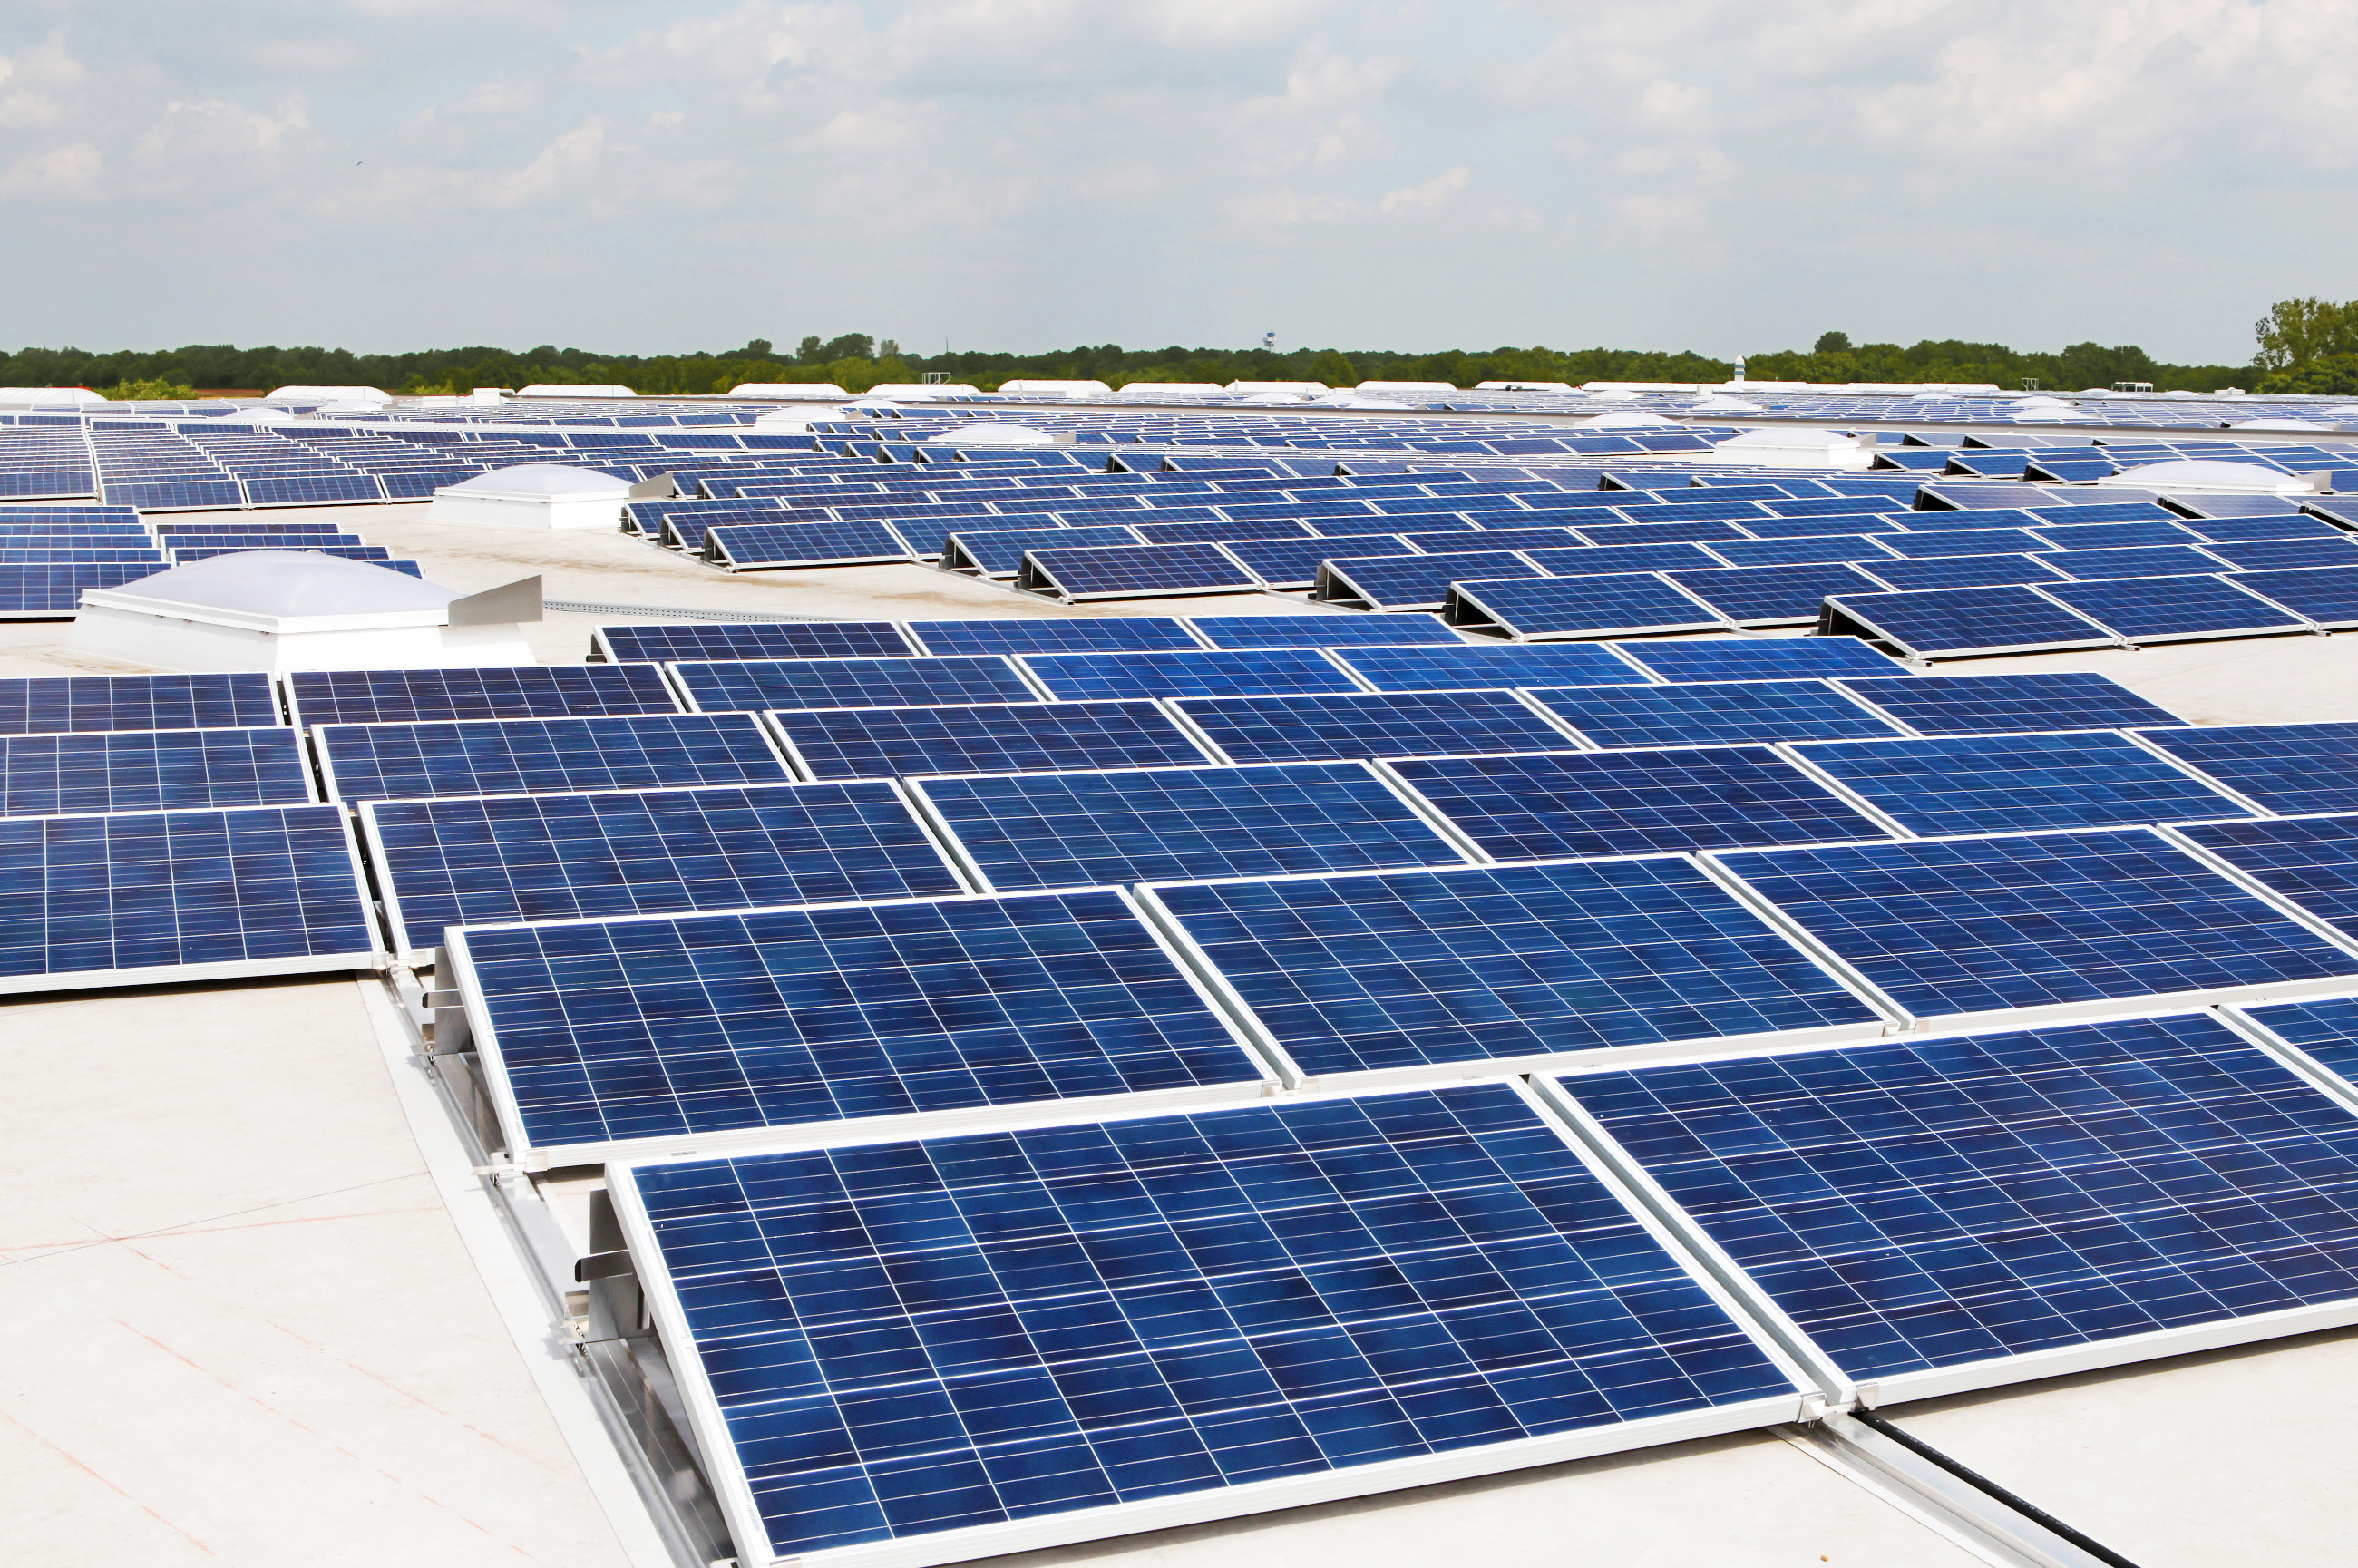
\includegraphics[width=\paperwidth,height=\paperheight]{images/titlepage/titlepic.jpg}%
        };
        %\node[
        %    fill=white,
        %    fill opacity=0.5,
        %    inner sep=0pt,
        %    anchor=west
        %] at (-38.5mm,-105mm) {%
        %    %% Creator: Matplotlib, PGF backend
%%
%% To include the figure in your LaTeX document, write
%%   \input{<filename>.pgf}
%%
%% Make sure the required packages are loaded in your preamble
%%   \usepackage{pgf}
%%
%% Figures using additional raster images can only be included by \input if
%% they are in the same directory as the main LaTeX file. For loading figures
%% from other directories you can use the `import` package
%%   \usepackage{import}
%% and then include the figures with
%%   \import{<path to file>}{<filename>.pgf}
%%
%% Matplotlib used the following preamble
%%   \usepackage{fontspec}
%%   \setmainfont{Bitstream Vera Serif}
%%   \setsansfont{Bitstream Vera Sans}
%%   \setmonofont{Bitstream Vera Sans Mono}
%%
\begingroup%
\makeatletter%
\begin{pgfpicture}%
\pgfpathrectangle{\pgfpointorigin}{\pgfqpoint{8.267700in}{2.000000in}}%
\pgfusepath{use as bounding box, clip}%
\begin{pgfscope}%
\pgfsetbuttcap%
\pgfsetmiterjoin%
\pgfsetlinewidth{0.000000pt}%
\definecolor{currentstroke}{rgb}{0.000000,0.000000,0.000000}%
\pgfsetstrokecolor{currentstroke}%
\pgfsetstrokeopacity{0.000000}%
\pgfsetdash{}{0pt}%
\pgfpathmoveto{\pgfqpoint{0.000000in}{0.000000in}}%
\pgfpathlineto{\pgfqpoint{8.267700in}{0.000000in}}%
\pgfpathlineto{\pgfqpoint{8.267700in}{2.000000in}}%
\pgfpathlineto{\pgfqpoint{0.000000in}{2.000000in}}%
\pgfpathclose%
\pgfusepath{}%
\end{pgfscope}%
\begin{pgfscope}%
\pgfsetbuttcap%
\pgfsetmiterjoin%
\pgfsetlinewidth{0.000000pt}%
\definecolor{currentstroke}{rgb}{0.000000,0.000000,0.000000}%
\pgfsetstrokecolor{currentstroke}%
\pgfsetstrokeopacity{0.000000}%
\pgfsetdash{}{0pt}%
\pgfpathmoveto{\pgfqpoint{0.826770in}{0.100000in}}%
\pgfpathlineto{\pgfqpoint{7.440930in}{0.100000in}}%
\pgfpathlineto{\pgfqpoint{7.440930in}{1.900000in}}%
\pgfpathlineto{\pgfqpoint{0.826770in}{1.900000in}}%
\pgfpathclose%
\pgfusepath{}%
\end{pgfscope}%
\begin{pgfscope}%
\pgfpathrectangle{\pgfqpoint{0.826770in}{0.100000in}}{\pgfqpoint{6.614160in}{1.800000in}} %
\pgfusepath{clip}%
\pgfsetroundcap%
\pgfsetroundjoin%
\pgfsetlinewidth{6.022500pt}%
\definecolor{currentstroke}{rgb}{0.500000,0.000000,0.000000}%
\pgfsetstrokecolor{currentstroke}%
\pgfsetdash{}{0pt}%
\pgfpathmoveto{\pgfqpoint{1.299210in}{1.000000in}}%
\pgfpathlineto{\pgfqpoint{1.333260in}{1.059662in}}%
\pgfpathlineto{\pgfqpoint{1.352176in}{1.088308in}}%
\pgfpathlineto{\pgfqpoint{1.367309in}{1.107297in}}%
\pgfpathlineto{\pgfqpoint{1.380551in}{1.120382in}}%
\pgfpathlineto{\pgfqpoint{1.391901in}{1.128645in}}%
\pgfpathlineto{\pgfqpoint{1.403251in}{1.133983in}}%
\pgfpathlineto{\pgfqpoint{1.412709in}{1.136107in}}%
\pgfpathlineto{\pgfqpoint{1.422167in}{1.136080in}}%
\pgfpathlineto{\pgfqpoint{1.431626in}{1.133903in}}%
\pgfpathlineto{\pgfqpoint{1.441084in}{1.129610in}}%
\pgfpathlineto{\pgfqpoint{1.452434in}{1.121763in}}%
\pgfpathlineto{\pgfqpoint{1.463784in}{1.111146in}}%
\pgfpathlineto{\pgfqpoint{1.477025in}{1.095586in}}%
\pgfpathlineto{\pgfqpoint{1.492158in}{1.074215in}}%
\pgfpathlineto{\pgfqpoint{1.511075in}{1.043401in}}%
\pgfpathlineto{\pgfqpoint{1.545125in}{0.982467in}}%
\pgfpathlineto{\pgfqpoint{1.571608in}{0.936892in}}%
\pgfpathlineto{\pgfqpoint{1.588633in}{0.911366in}}%
\pgfpathlineto{\pgfqpoint{1.603766in}{0.892438in}}%
\pgfpathlineto{\pgfqpoint{1.617007in}{0.879417in}}%
\pgfpathlineto{\pgfqpoint{1.628357in}{0.871213in}}%
\pgfpathlineto{\pgfqpoint{1.639707in}{0.865937in}}%
\pgfpathlineto{\pgfqpoint{1.649166in}{0.863867in}}%
\pgfpathlineto{\pgfqpoint{1.658624in}{0.863948in}}%
\pgfpathlineto{\pgfqpoint{1.668082in}{0.866179in}}%
\pgfpathlineto{\pgfqpoint{1.677540in}{0.870524in}}%
\pgfpathlineto{\pgfqpoint{1.688890in}{0.878431in}}%
\pgfpathlineto{\pgfqpoint{1.700240in}{0.889103in}}%
\pgfpathlineto{\pgfqpoint{1.713482in}{0.904720in}}%
\pgfpathlineto{\pgfqpoint{1.728615in}{0.926145in}}%
\pgfpathlineto{\pgfqpoint{1.747531in}{0.957006in}}%
\pgfpathlineto{\pgfqpoint{1.781581in}{1.017958in}}%
\pgfpathlineto{\pgfqpoint{1.808064in}{1.063488in}}%
\pgfpathlineto{\pgfqpoint{1.825089in}{1.088960in}}%
\pgfpathlineto{\pgfqpoint{1.840222in}{1.107825in}}%
\pgfpathlineto{\pgfqpoint{1.853464in}{1.120782in}}%
\pgfpathlineto{\pgfqpoint{1.864814in}{1.128927in}}%
\pgfpathlineto{\pgfqpoint{1.876164in}{1.134140in}}%
\pgfpathlineto{\pgfqpoint{1.885622in}{1.136157in}}%
\pgfpathlineto{\pgfqpoint{1.895080in}{1.136022in}}%
\pgfpathlineto{\pgfqpoint{1.904539in}{1.133738in}}%
\pgfpathlineto{\pgfqpoint{1.913997in}{1.129341in}}%
\pgfpathlineto{\pgfqpoint{1.925347in}{1.121374in}}%
\pgfpathlineto{\pgfqpoint{1.936697in}{1.110647in}}%
\pgfpathlineto{\pgfqpoint{1.949938in}{1.094973in}}%
\pgfpathlineto{\pgfqpoint{1.965071in}{1.073494in}}%
\pgfpathlineto{\pgfqpoint{1.983988in}{1.042587in}}%
\pgfpathlineto{\pgfqpoint{2.019929in}{0.978223in}}%
\pgfpathlineto{\pgfqpoint{2.046412in}{0.933122in}}%
\pgfpathlineto{\pgfqpoint{2.063437in}{0.908151in}}%
\pgfpathlineto{\pgfqpoint{2.078570in}{0.889856in}}%
\pgfpathlineto{\pgfqpoint{2.091812in}{0.877475in}}%
\pgfpathlineto{\pgfqpoint{2.103162in}{0.869867in}}%
\pgfpathlineto{\pgfqpoint{2.112620in}{0.865783in}}%
\pgfpathlineto{\pgfqpoint{2.122078in}{0.863820in}}%
\pgfpathlineto{\pgfqpoint{2.131537in}{0.864009in}}%
\pgfpathlineto{\pgfqpoint{2.140995in}{0.866346in}}%
\pgfpathlineto{\pgfqpoint{2.150453in}{0.870796in}}%
\pgfpathlineto{\pgfqpoint{2.161803in}{0.878822in}}%
\pgfpathlineto{\pgfqpoint{2.173153in}{0.889604in}}%
\pgfpathlineto{\pgfqpoint{2.186395in}{0.905336in}}%
\pgfpathlineto{\pgfqpoint{2.201528in}{0.926868in}}%
\pgfpathlineto{\pgfqpoint{2.220444in}{0.957821in}}%
\pgfpathlineto{\pgfqpoint{2.256386in}{1.022200in}}%
\pgfpathlineto{\pgfqpoint{2.282869in}{1.067251in}}%
\pgfpathlineto{\pgfqpoint{2.299894in}{1.092165in}}%
\pgfpathlineto{\pgfqpoint{2.315027in}{1.110396in}}%
\pgfpathlineto{\pgfqpoint{2.328268in}{1.122713in}}%
\pgfpathlineto{\pgfqpoint{2.339618in}{1.130260in}}%
\pgfpathlineto{\pgfqpoint{2.349077in}{1.134292in}}%
\pgfpathlineto{\pgfqpoint{2.358535in}{1.136202in}}%
\pgfpathlineto{\pgfqpoint{2.367993in}{1.135959in}}%
\pgfpathlineto{\pgfqpoint{2.377451in}{1.133568in}}%
\pgfpathlineto{\pgfqpoint{2.386910in}{1.129066in}}%
\pgfpathlineto{\pgfqpoint{2.398260in}{1.120981in}}%
\pgfpathlineto{\pgfqpoint{2.409610in}{1.110144in}}%
\pgfpathlineto{\pgfqpoint{2.422851in}{1.094355in}}%
\pgfpathlineto{\pgfqpoint{2.437984in}{1.072770in}}%
\pgfpathlineto{\pgfqpoint{2.456901in}{1.041771in}}%
\pgfpathlineto{\pgfqpoint{2.494734in}{0.974002in}}%
\pgfpathlineto{\pgfqpoint{2.519325in}{0.932376in}}%
\pgfpathlineto{\pgfqpoint{2.536350in}{0.907519in}}%
\pgfpathlineto{\pgfqpoint{2.551483in}{0.889353in}}%
\pgfpathlineto{\pgfqpoint{2.564725in}{0.877101in}}%
\pgfpathlineto{\pgfqpoint{2.576075in}{0.869614in}}%
\pgfpathlineto{\pgfqpoint{2.585533in}{0.865634in}}%
\pgfpathlineto{\pgfqpoint{2.594991in}{0.863778in}}%
\pgfpathlineto{\pgfqpoint{2.604450in}{0.864075in}}%
\pgfpathlineto{\pgfqpoint{2.613908in}{0.866519in}}%
\pgfpathlineto{\pgfqpoint{2.623366in}{0.871073in}}%
\pgfpathlineto{\pgfqpoint{2.634716in}{0.879218in}}%
\pgfpathlineto{\pgfqpoint{2.646066in}{0.890110in}}%
\pgfpathlineto{\pgfqpoint{2.659308in}{0.905955in}}%
\pgfpathlineto{\pgfqpoint{2.674441in}{0.927593in}}%
\pgfpathlineto{\pgfqpoint{2.693357in}{0.958637in}}%
\pgfpathlineto{\pgfqpoint{2.733082in}{1.029776in}}%
\pgfpathlineto{\pgfqpoint{2.757673in}{1.070948in}}%
\pgfpathlineto{\pgfqpoint{2.774698in}{1.095280in}}%
\pgfpathlineto{\pgfqpoint{2.787940in}{1.110897in}}%
\pgfpathlineto{\pgfqpoint{2.801181in}{1.123084in}}%
\pgfpathlineto{\pgfqpoint{2.812531in}{1.130511in}}%
\pgfpathlineto{\pgfqpoint{2.821990in}{1.134438in}}%
\pgfpathlineto{\pgfqpoint{2.831448in}{1.136241in}}%
\pgfpathlineto{\pgfqpoint{2.840906in}{1.135890in}}%
\pgfpathlineto{\pgfqpoint{2.850364in}{1.133393in}}%
\pgfpathlineto{\pgfqpoint{2.859823in}{1.128787in}}%
\pgfpathlineto{\pgfqpoint{2.871173in}{1.120583in}}%
\pgfpathlineto{\pgfqpoint{2.882522in}{1.109636in}}%
\pgfpathlineto{\pgfqpoint{2.895764in}{1.093734in}}%
\pgfpathlineto{\pgfqpoint{2.910897in}{1.072043in}}%
\pgfpathlineto{\pgfqpoint{2.929814in}{1.040954in}}%
\pgfpathlineto{\pgfqpoint{2.971430in}{0.966470in}}%
\pgfpathlineto{\pgfqpoint{2.994130in}{0.928686in}}%
\pgfpathlineto{\pgfqpoint{3.011155in}{0.904414in}}%
\pgfpathlineto{\pgfqpoint{3.024396in}{0.888854in}}%
\pgfpathlineto{\pgfqpoint{3.037638in}{0.876732in}}%
\pgfpathlineto{\pgfqpoint{3.048988in}{0.869365in}}%
\pgfpathlineto{\pgfqpoint{3.058446in}{0.865491in}}%
\pgfpathlineto{\pgfqpoint{3.067904in}{0.863742in}}%
\pgfpathlineto{\pgfqpoint{3.077363in}{0.864146in}}%
\pgfpathlineto{\pgfqpoint{3.086821in}{0.866697in}}%
\pgfpathlineto{\pgfqpoint{3.096279in}{0.871355in}}%
\pgfpathlineto{\pgfqpoint{3.107629in}{0.879618in}}%
\pgfpathlineto{\pgfqpoint{3.118979in}{0.890620in}}%
\pgfpathlineto{\pgfqpoint{3.132220in}{0.906578in}}%
\pgfpathlineto{\pgfqpoint{3.147354in}{0.928321in}}%
\pgfpathlineto{\pgfqpoint{3.166270in}{0.959455in}}%
\pgfpathlineto{\pgfqpoint{3.188970in}{1.000000in}}%
\pgfpathlineto{\pgfqpoint{3.188970in}{1.000000in}}%
\pgfusepath{stroke}%
\end{pgfscope}%
\begin{pgfscope}%
\pgfpathrectangle{\pgfqpoint{0.826770in}{0.100000in}}{\pgfqpoint{6.614160in}{1.800000in}} %
\pgfusepath{clip}%
\pgfsetroundcap%
\pgfsetroundjoin%
\pgfsetlinewidth{6.022500pt}%
\definecolor{currentstroke}{rgb}{0.500000,0.000000,0.000000}%
\pgfsetstrokecolor{currentstroke}%
\pgfsetdash{}{0pt}%
\pgfpathmoveto{\pgfqpoint{3.188970in}{1.000000in}}%
\pgfpathlineto{\pgfqpoint{3.221128in}{1.339353in}}%
\pgfpathlineto{\pgfqpoint{3.238153in}{1.497822in}}%
\pgfpathlineto{\pgfqpoint{3.251395in}{1.603878in}}%
\pgfpathlineto{\pgfqpoint{3.262744in}{1.680025in}}%
\pgfpathlineto{\pgfqpoint{3.272203in}{1.731730in}}%
\pgfpathlineto{\pgfqpoint{3.281661in}{1.771873in}}%
\pgfpathlineto{\pgfqpoint{3.289228in}{1.795229in}}%
\pgfpathlineto{\pgfqpoint{3.294902in}{1.807475in}}%
\pgfpathlineto{\pgfqpoint{3.300577in}{1.815124in}}%
\pgfpathlineto{\pgfqpoint{3.304361in}{1.817647in}}%
\pgfpathlineto{\pgfqpoint{3.308144in}{1.818100in}}%
\pgfpathlineto{\pgfqpoint{3.311927in}{1.816482in}}%
\pgfpathlineto{\pgfqpoint{3.315711in}{1.812798in}}%
\pgfpathlineto{\pgfqpoint{3.321386in}{1.803418in}}%
\pgfpathlineto{\pgfqpoint{3.327061in}{1.789464in}}%
\pgfpathlineto{\pgfqpoint{3.334627in}{1.763885in}}%
\pgfpathlineto{\pgfqpoint{3.342194in}{1.730576in}}%
\pgfpathlineto{\pgfqpoint{3.351652in}{1.678591in}}%
\pgfpathlineto{\pgfqpoint{3.363002in}{1.602139in}}%
\pgfpathlineto{\pgfqpoint{3.376244in}{1.495778in}}%
\pgfpathlineto{\pgfqpoint{3.391377in}{1.355658in}}%
\pgfpathlineto{\pgfqpoint{3.412185in}{1.140809in}}%
\pgfpathlineto{\pgfqpoint{3.463259in}{0.603225in}}%
\pgfpathlineto{\pgfqpoint{3.480284in}{0.452721in}}%
\pgfpathlineto{\pgfqpoint{3.493526in}{0.354631in}}%
\pgfpathlineto{\pgfqpoint{3.504876in}{0.286344in}}%
\pgfpathlineto{\pgfqpoint{3.514334in}{0.241781in}}%
\pgfpathlineto{\pgfqpoint{3.521901in}{0.214730in}}%
\pgfpathlineto{\pgfqpoint{3.529467in}{0.195624in}}%
\pgfpathlineto{\pgfqpoint{3.535142in}{0.186629in}}%
\pgfpathlineto{\pgfqpoint{3.540817in}{0.182264in}}%
\pgfpathlineto{\pgfqpoint{3.544601in}{0.181941in}}%
\pgfpathlineto{\pgfqpoint{3.548384in}{0.183688in}}%
\pgfpathlineto{\pgfqpoint{3.552167in}{0.187501in}}%
\pgfpathlineto{\pgfqpoint{3.557842in}{0.197072in}}%
\pgfpathlineto{\pgfqpoint{3.563517in}{0.211215in}}%
\pgfpathlineto{\pgfqpoint{3.571084in}{0.237041in}}%
\pgfpathlineto{\pgfqpoint{3.578650in}{0.270586in}}%
\pgfpathlineto{\pgfqpoint{3.588108in}{0.322850in}}%
\pgfpathlineto{\pgfqpoint{3.599458in}{0.399606in}}%
\pgfpathlineto{\pgfqpoint{3.612700in}{0.506271in}}%
\pgfpathlineto{\pgfqpoint{3.627833in}{0.646661in}}%
\pgfpathlineto{\pgfqpoint{3.648641in}{0.861727in}}%
\pgfpathlineto{\pgfqpoint{3.699716in}{1.399023in}}%
\pgfpathlineto{\pgfqpoint{3.716741in}{1.549189in}}%
\pgfpathlineto{\pgfqpoint{3.729982in}{1.646948in}}%
\pgfpathlineto{\pgfqpoint{3.741332in}{1.714911in}}%
\pgfpathlineto{\pgfqpoint{3.750791in}{1.759182in}}%
\pgfpathlineto{\pgfqpoint{3.758357in}{1.785988in}}%
\pgfpathlineto{\pgfqpoint{3.765924in}{1.804842in}}%
\pgfpathlineto{\pgfqpoint{3.771599in}{1.813646in}}%
\pgfpathlineto{\pgfqpoint{3.777274in}{1.817817in}}%
\pgfpathlineto{\pgfqpoint{3.781057in}{1.818011in}}%
\pgfpathlineto{\pgfqpoint{3.784840in}{1.816135in}}%
\pgfpathlineto{\pgfqpoint{3.788624in}{1.812192in}}%
\pgfpathlineto{\pgfqpoint{3.794299in}{1.802429in}}%
\pgfpathlineto{\pgfqpoint{3.799973in}{1.788097in}}%
\pgfpathlineto{\pgfqpoint{3.807540in}{1.762026in}}%
\pgfpathlineto{\pgfqpoint{3.815107in}{1.728245in}}%
\pgfpathlineto{\pgfqpoint{3.824565in}{1.675703in}}%
\pgfpathlineto{\pgfqpoint{3.835915in}{1.598643in}}%
\pgfpathlineto{\pgfqpoint{3.849156in}{1.491675in}}%
\pgfpathlineto{\pgfqpoint{3.864290in}{1.351017in}}%
\pgfpathlineto{\pgfqpoint{3.885098in}{1.135737in}}%
\pgfpathlineto{\pgfqpoint{3.934281in}{0.616796in}}%
\pgfpathlineto{\pgfqpoint{3.951306in}{0.464293in}}%
\pgfpathlineto{\pgfqpoint{3.964547in}{0.364234in}}%
\pgfpathlineto{\pgfqpoint{3.975897in}{0.294021in}}%
\pgfpathlineto{\pgfqpoint{3.985355in}{0.247717in}}%
\pgfpathlineto{\pgfqpoint{3.992922in}{0.219204in}}%
\pgfpathlineto{\pgfqpoint{4.000489in}{0.198591in}}%
\pgfpathlineto{\pgfqpoint{4.006164in}{0.188445in}}%
\pgfpathlineto{\pgfqpoint{4.011838in}{0.182919in}}%
\pgfpathlineto{\pgfqpoint{4.015622in}{0.181819in}}%
\pgfpathlineto{\pgfqpoint{4.019405in}{0.182790in}}%
\pgfpathlineto{\pgfqpoint{4.023188in}{0.185829in}}%
\pgfpathlineto{\pgfqpoint{4.028863in}{0.194248in}}%
\pgfpathlineto{\pgfqpoint{4.034538in}{0.207255in}}%
\pgfpathlineto{\pgfqpoint{4.042105in}{0.231602in}}%
\pgfpathlineto{\pgfqpoint{4.049672in}{0.263723in}}%
\pgfpathlineto{\pgfqpoint{4.059130in}{0.314306in}}%
\pgfpathlineto{\pgfqpoint{4.070480in}{0.389225in}}%
\pgfpathlineto{\pgfqpoint{4.083721in}{0.494050in}}%
\pgfpathlineto{\pgfqpoint{4.098854in}{0.632801in}}%
\pgfpathlineto{\pgfqpoint{4.119663in}{0.846536in}}%
\pgfpathlineto{\pgfqpoint{4.172629in}{1.403508in}}%
\pgfpathlineto{\pgfqpoint{4.187762in}{1.537649in}}%
\pgfpathlineto{\pgfqpoint{4.201004in}{1.637382in}}%
\pgfpathlineto{\pgfqpoint{4.212354in}{1.707276in}}%
\pgfpathlineto{\pgfqpoint{4.221812in}{1.753291in}}%
\pgfpathlineto{\pgfqpoint{4.229378in}{1.781561in}}%
\pgfpathlineto{\pgfqpoint{4.236945in}{1.801923in}}%
\pgfpathlineto{\pgfqpoint{4.242620in}{1.811878in}}%
\pgfpathlineto{\pgfqpoint{4.248295in}{1.817210in}}%
\pgfpathlineto{\pgfqpoint{4.252078in}{1.818181in}}%
\pgfpathlineto{\pgfqpoint{4.255862in}{1.817081in}}%
\pgfpathlineto{\pgfqpoint{4.259645in}{1.813912in}}%
\pgfpathlineto{\pgfqpoint{4.265320in}{1.805301in}}%
\pgfpathlineto{\pgfqpoint{4.270995in}{1.792105in}}%
\pgfpathlineto{\pgfqpoint{4.278561in}{1.767511in}}%
\pgfpathlineto{\pgfqpoint{4.286128in}{1.735151in}}%
\pgfpathlineto{\pgfqpoint{4.295586in}{1.684287in}}%
\pgfpathlineto{\pgfqpoint{4.306936in}{1.609059in}}%
\pgfpathlineto{\pgfqpoint{4.320178in}{1.503926in}}%
\pgfpathlineto{\pgfqpoint{4.335311in}{1.364898in}}%
\pgfpathlineto{\pgfqpoint{4.356119in}{1.150936in}}%
\pgfpathlineto{\pgfqpoint{4.409085in}{0.594256in}}%
\pgfpathlineto{\pgfqpoint{4.424219in}{0.460414in}}%
\pgfpathlineto{\pgfqpoint{4.437460in}{0.361008in}}%
\pgfpathlineto{\pgfqpoint{4.448810in}{0.291434in}}%
\pgfpathlineto{\pgfqpoint{4.458268in}{0.245708in}}%
\pgfpathlineto{\pgfqpoint{4.465835in}{0.217682in}}%
\pgfpathlineto{\pgfqpoint{4.473401in}{0.197571in}}%
\pgfpathlineto{\pgfqpoint{4.479076in}{0.187808in}}%
\pgfpathlineto{\pgfqpoint{4.484751in}{0.182669in}}%
\pgfpathlineto{\pgfqpoint{4.488535in}{0.181827in}}%
\pgfpathlineto{\pgfqpoint{4.492318in}{0.183057in}}%
\pgfpathlineto{\pgfqpoint{4.496101in}{0.186354in}}%
\pgfpathlineto{\pgfqpoint{4.501776in}{0.195158in}}%
\pgfpathlineto{\pgfqpoint{4.507451in}{0.208544in}}%
\pgfpathlineto{\pgfqpoint{4.515018in}{0.233384in}}%
\pgfpathlineto{\pgfqpoint{4.522584in}{0.265982in}}%
\pgfpathlineto{\pgfqpoint{4.532043in}{0.317127in}}%
\pgfpathlineto{\pgfqpoint{4.543393in}{0.392662in}}%
\pgfpathlineto{\pgfqpoint{4.556634in}{0.498104in}}%
\pgfpathlineto{\pgfqpoint{4.571767in}{0.637406in}}%
\pgfpathlineto{\pgfqpoint{4.592576in}{0.851594in}}%
\pgfpathlineto{\pgfqpoint{4.645542in}{1.407976in}}%
\pgfpathlineto{\pgfqpoint{4.660675in}{1.541517in}}%
\pgfpathlineto{\pgfqpoint{4.673917in}{1.640596in}}%
\pgfpathlineto{\pgfqpoint{4.685266in}{1.709849in}}%
\pgfpathlineto{\pgfqpoint{4.694725in}{1.755285in}}%
\pgfpathlineto{\pgfqpoint{4.702291in}{1.783068in}}%
\pgfpathlineto{\pgfqpoint{4.709858in}{1.802928in}}%
\pgfpathlineto{\pgfqpoint{4.715533in}{1.812499in}}%
\pgfpathlineto{\pgfqpoint{4.721208in}{1.817445in}}%
\pgfpathlineto{\pgfqpoint{4.724991in}{1.818157in}}%
\pgfpathlineto{\pgfqpoint{4.728774in}{1.816798in}}%
\pgfpathlineto{\pgfqpoint{4.732558in}{1.813371in}}%
\pgfpathlineto{\pgfqpoint{4.738233in}{1.804376in}}%
\pgfpathlineto{\pgfqpoint{4.743908in}{1.790800in}}%
\pgfpathlineto{\pgfqpoint{4.751474in}{1.765713in}}%
\pgfpathlineto{\pgfqpoint{4.759041in}{1.732878in}}%
\pgfpathlineto{\pgfqpoint{4.768499in}{1.681453in}}%
\pgfpathlineto{\pgfqpoint{4.779849in}{1.605611in}}%
\pgfpathlineto{\pgfqpoint{4.793091in}{1.499862in}}%
\pgfpathlineto{\pgfqpoint{4.808224in}{1.360285in}}%
\pgfpathlineto{\pgfqpoint{4.829032in}{1.145875in}}%
\pgfpathlineto{\pgfqpoint{4.880107in}{0.607733in}}%
\pgfpathlineto{\pgfqpoint{4.897131in}{0.456557in}}%
\pgfpathlineto{\pgfqpoint{4.910373in}{0.357807in}}%
\pgfpathlineto{\pgfqpoint{4.921723in}{0.288875in}}%
\pgfpathlineto{\pgfqpoint{4.931181in}{0.243730in}}%
\pgfpathlineto{\pgfqpoint{4.938748in}{0.216190in}}%
\pgfpathlineto{\pgfqpoint{4.946314in}{0.196582in}}%
\pgfpathlineto{\pgfqpoint{4.951989in}{0.187202in}}%
\pgfpathlineto{\pgfqpoint{4.957664in}{0.182450in}}%
\pgfpathlineto{\pgfqpoint{4.961448in}{0.181868in}}%
\pgfpathlineto{\pgfqpoint{4.965231in}{0.183356in}}%
\pgfpathlineto{\pgfqpoint{4.969014in}{0.186911in}}%
\pgfpathlineto{\pgfqpoint{4.974689in}{0.196099in}}%
\pgfpathlineto{\pgfqpoint{4.980364in}{0.209864in}}%
\pgfpathlineto{\pgfqpoint{4.987931in}{0.235197in}}%
\pgfpathlineto{\pgfqpoint{4.995497in}{0.268270in}}%
\pgfpathlineto{\pgfqpoint{5.004956in}{0.319975in}}%
\pgfpathlineto{\pgfqpoint{5.016305in}{0.396122in}}%
\pgfpathlineto{\pgfqpoint{5.029547in}{0.502178in}}%
\pgfpathlineto{\pgfqpoint{5.044680in}{0.642027in}}%
\pgfpathlineto{\pgfqpoint{5.065488in}{0.856657in}}%
\pgfpathlineto{\pgfqpoint{5.078730in}{1.000000in}}%
\pgfpathlineto{\pgfqpoint{5.078730in}{1.000000in}}%
\pgfusepath{stroke}%
\end{pgfscope}%
\begin{pgfscope}%
\pgfpathrectangle{\pgfqpoint{0.826770in}{0.100000in}}{\pgfqpoint{6.614160in}{1.800000in}} %
\pgfusepath{clip}%
\pgfsetroundcap%
\pgfsetroundjoin%
\pgfsetlinewidth{6.022500pt}%
\definecolor{currentstroke}{rgb}{0.500000,0.000000,0.000000}%
\pgfsetstrokecolor{currentstroke}%
\pgfsetdash{}{0pt}%
\pgfpathmoveto{\pgfqpoint{5.078730in}{1.000000in}}%
\pgfpathlineto{\pgfqpoint{5.112780in}{1.059662in}}%
\pgfpathlineto{\pgfqpoint{5.131696in}{1.088308in}}%
\pgfpathlineto{\pgfqpoint{5.146829in}{1.107297in}}%
\pgfpathlineto{\pgfqpoint{5.160071in}{1.120382in}}%
\pgfpathlineto{\pgfqpoint{5.171421in}{1.128645in}}%
\pgfpathlineto{\pgfqpoint{5.182771in}{1.133983in}}%
\pgfpathlineto{\pgfqpoint{5.192229in}{1.136107in}}%
\pgfpathlineto{\pgfqpoint{5.201687in}{1.136080in}}%
\pgfpathlineto{\pgfqpoint{5.211146in}{1.133903in}}%
\pgfpathlineto{\pgfqpoint{5.220604in}{1.129610in}}%
\pgfpathlineto{\pgfqpoint{5.231954in}{1.121763in}}%
\pgfpathlineto{\pgfqpoint{5.243304in}{1.111146in}}%
\pgfpathlineto{\pgfqpoint{5.256545in}{1.095586in}}%
\pgfpathlineto{\pgfqpoint{5.271678in}{1.074215in}}%
\pgfpathlineto{\pgfqpoint{5.290595in}{1.043401in}}%
\pgfpathlineto{\pgfqpoint{5.324645in}{0.982467in}}%
\pgfpathlineto{\pgfqpoint{5.351128in}{0.936892in}}%
\pgfpathlineto{\pgfqpoint{5.368153in}{0.911366in}}%
\pgfpathlineto{\pgfqpoint{5.383286in}{0.892438in}}%
\pgfpathlineto{\pgfqpoint{5.396527in}{0.879417in}}%
\pgfpathlineto{\pgfqpoint{5.407877in}{0.871213in}}%
\pgfpathlineto{\pgfqpoint{5.419227in}{0.865937in}}%
\pgfpathlineto{\pgfqpoint{5.428686in}{0.863867in}}%
\pgfpathlineto{\pgfqpoint{5.438144in}{0.863948in}}%
\pgfpathlineto{\pgfqpoint{5.447602in}{0.866179in}}%
\pgfpathlineto{\pgfqpoint{5.457060in}{0.870524in}}%
\pgfpathlineto{\pgfqpoint{5.468410in}{0.878431in}}%
\pgfpathlineto{\pgfqpoint{5.479760in}{0.889103in}}%
\pgfpathlineto{\pgfqpoint{5.493002in}{0.904720in}}%
\pgfpathlineto{\pgfqpoint{5.508135in}{0.926145in}}%
\pgfpathlineto{\pgfqpoint{5.527051in}{0.957006in}}%
\pgfpathlineto{\pgfqpoint{5.561101in}{1.017958in}}%
\pgfpathlineto{\pgfqpoint{5.587584in}{1.063488in}}%
\pgfpathlineto{\pgfqpoint{5.604609in}{1.088960in}}%
\pgfpathlineto{\pgfqpoint{5.619742in}{1.107825in}}%
\pgfpathlineto{\pgfqpoint{5.632984in}{1.120782in}}%
\pgfpathlineto{\pgfqpoint{5.644334in}{1.128927in}}%
\pgfpathlineto{\pgfqpoint{5.655684in}{1.134140in}}%
\pgfpathlineto{\pgfqpoint{5.665142in}{1.136157in}}%
\pgfpathlineto{\pgfqpoint{5.674600in}{1.136022in}}%
\pgfpathlineto{\pgfqpoint{5.684059in}{1.133738in}}%
\pgfpathlineto{\pgfqpoint{5.693517in}{1.129341in}}%
\pgfpathlineto{\pgfqpoint{5.704867in}{1.121374in}}%
\pgfpathlineto{\pgfqpoint{5.716217in}{1.110647in}}%
\pgfpathlineto{\pgfqpoint{5.729458in}{1.094973in}}%
\pgfpathlineto{\pgfqpoint{5.744591in}{1.073494in}}%
\pgfpathlineto{\pgfqpoint{5.763508in}{1.042587in}}%
\pgfpathlineto{\pgfqpoint{5.799449in}{0.978223in}}%
\pgfpathlineto{\pgfqpoint{5.825932in}{0.933122in}}%
\pgfpathlineto{\pgfqpoint{5.842957in}{0.908151in}}%
\pgfpathlineto{\pgfqpoint{5.858090in}{0.889856in}}%
\pgfpathlineto{\pgfqpoint{5.871332in}{0.877475in}}%
\pgfpathlineto{\pgfqpoint{5.882682in}{0.869867in}}%
\pgfpathlineto{\pgfqpoint{5.892140in}{0.865783in}}%
\pgfpathlineto{\pgfqpoint{5.901598in}{0.863820in}}%
\pgfpathlineto{\pgfqpoint{5.911057in}{0.864009in}}%
\pgfpathlineto{\pgfqpoint{5.920515in}{0.866346in}}%
\pgfpathlineto{\pgfqpoint{5.929973in}{0.870796in}}%
\pgfpathlineto{\pgfqpoint{5.941323in}{0.878822in}}%
\pgfpathlineto{\pgfqpoint{5.952673in}{0.889604in}}%
\pgfpathlineto{\pgfqpoint{5.965915in}{0.905336in}}%
\pgfpathlineto{\pgfqpoint{5.981048in}{0.926868in}}%
\pgfpathlineto{\pgfqpoint{5.999964in}{0.957821in}}%
\pgfpathlineto{\pgfqpoint{6.035906in}{1.022200in}}%
\pgfpathlineto{\pgfqpoint{6.062389in}{1.067251in}}%
\pgfpathlineto{\pgfqpoint{6.079414in}{1.092165in}}%
\pgfpathlineto{\pgfqpoint{6.094547in}{1.110396in}}%
\pgfpathlineto{\pgfqpoint{6.107788in}{1.122713in}}%
\pgfpathlineto{\pgfqpoint{6.119138in}{1.130260in}}%
\pgfpathlineto{\pgfqpoint{6.128597in}{1.134292in}}%
\pgfpathlineto{\pgfqpoint{6.138055in}{1.136202in}}%
\pgfpathlineto{\pgfqpoint{6.147513in}{1.135959in}}%
\pgfpathlineto{\pgfqpoint{6.156971in}{1.133568in}}%
\pgfpathlineto{\pgfqpoint{6.166430in}{1.129066in}}%
\pgfpathlineto{\pgfqpoint{6.177780in}{1.120981in}}%
\pgfpathlineto{\pgfqpoint{6.189130in}{1.110144in}}%
\pgfpathlineto{\pgfqpoint{6.202371in}{1.094355in}}%
\pgfpathlineto{\pgfqpoint{6.217504in}{1.072770in}}%
\pgfpathlineto{\pgfqpoint{6.236421in}{1.041771in}}%
\pgfpathlineto{\pgfqpoint{6.274254in}{0.974002in}}%
\pgfpathlineto{\pgfqpoint{6.298845in}{0.932376in}}%
\pgfpathlineto{\pgfqpoint{6.315870in}{0.907519in}}%
\pgfpathlineto{\pgfqpoint{6.331003in}{0.889353in}}%
\pgfpathlineto{\pgfqpoint{6.344245in}{0.877101in}}%
\pgfpathlineto{\pgfqpoint{6.355595in}{0.869614in}}%
\pgfpathlineto{\pgfqpoint{6.365053in}{0.865634in}}%
\pgfpathlineto{\pgfqpoint{6.374511in}{0.863778in}}%
\pgfpathlineto{\pgfqpoint{6.383970in}{0.864075in}}%
\pgfpathlineto{\pgfqpoint{6.393428in}{0.866519in}}%
\pgfpathlineto{\pgfqpoint{6.402886in}{0.871073in}}%
\pgfpathlineto{\pgfqpoint{6.414236in}{0.879218in}}%
\pgfpathlineto{\pgfqpoint{6.425586in}{0.890110in}}%
\pgfpathlineto{\pgfqpoint{6.438828in}{0.905955in}}%
\pgfpathlineto{\pgfqpoint{6.453961in}{0.927593in}}%
\pgfpathlineto{\pgfqpoint{6.472877in}{0.958637in}}%
\pgfpathlineto{\pgfqpoint{6.512602in}{1.029776in}}%
\pgfpathlineto{\pgfqpoint{6.537193in}{1.070948in}}%
\pgfpathlineto{\pgfqpoint{6.554218in}{1.095280in}}%
\pgfpathlineto{\pgfqpoint{6.567460in}{1.110897in}}%
\pgfpathlineto{\pgfqpoint{6.580701in}{1.123084in}}%
\pgfpathlineto{\pgfqpoint{6.592051in}{1.130511in}}%
\pgfpathlineto{\pgfqpoint{6.601510in}{1.134438in}}%
\pgfpathlineto{\pgfqpoint{6.610968in}{1.136241in}}%
\pgfpathlineto{\pgfqpoint{6.620426in}{1.135890in}}%
\pgfpathlineto{\pgfqpoint{6.629884in}{1.133393in}}%
\pgfpathlineto{\pgfqpoint{6.639343in}{1.128787in}}%
\pgfpathlineto{\pgfqpoint{6.650693in}{1.120583in}}%
\pgfpathlineto{\pgfqpoint{6.662042in}{1.109636in}}%
\pgfpathlineto{\pgfqpoint{6.675284in}{1.093734in}}%
\pgfpathlineto{\pgfqpoint{6.690417in}{1.072043in}}%
\pgfpathlineto{\pgfqpoint{6.709334in}{1.040954in}}%
\pgfpathlineto{\pgfqpoint{6.750950in}{0.966470in}}%
\pgfpathlineto{\pgfqpoint{6.773650in}{0.928686in}}%
\pgfpathlineto{\pgfqpoint{6.790675in}{0.904414in}}%
\pgfpathlineto{\pgfqpoint{6.803916in}{0.888854in}}%
\pgfpathlineto{\pgfqpoint{6.817158in}{0.876732in}}%
\pgfpathlineto{\pgfqpoint{6.828508in}{0.869365in}}%
\pgfpathlineto{\pgfqpoint{6.837966in}{0.865491in}}%
\pgfpathlineto{\pgfqpoint{6.847424in}{0.863742in}}%
\pgfpathlineto{\pgfqpoint{6.856883in}{0.864146in}}%
\pgfpathlineto{\pgfqpoint{6.866341in}{0.866697in}}%
\pgfpathlineto{\pgfqpoint{6.875799in}{0.871355in}}%
\pgfpathlineto{\pgfqpoint{6.887149in}{0.879618in}}%
\pgfpathlineto{\pgfqpoint{6.898499in}{0.890620in}}%
\pgfpathlineto{\pgfqpoint{6.911740in}{0.906578in}}%
\pgfpathlineto{\pgfqpoint{6.926874in}{0.928321in}}%
\pgfpathlineto{\pgfqpoint{6.945790in}{0.959455in}}%
\pgfpathlineto{\pgfqpoint{6.968490in}{1.000000in}}%
\pgfpathlineto{\pgfqpoint{6.968490in}{1.000000in}}%
\pgfusepath{stroke}%
\end{pgfscope}%
\begin{pgfscope}%
\pgfpathrectangle{\pgfqpoint{0.826770in}{0.100000in}}{\pgfqpoint{6.614160in}{1.800000in}} %
\pgfusepath{clip}%
\pgfsetroundcap%
\pgfsetroundjoin%
\pgfsetlinewidth{4.015000pt}%
\definecolor{currentstroke}{rgb}{0.750000,0.000000,0.000000}%
\pgfsetstrokecolor{currentstroke}%
\pgfsetdash{}{0pt}%
\pgfpathmoveto{\pgfqpoint{1.299210in}{1.000000in}}%
\pgfpathlineto{\pgfqpoint{1.333260in}{1.059662in}}%
\pgfpathlineto{\pgfqpoint{1.352176in}{1.088308in}}%
\pgfpathlineto{\pgfqpoint{1.367309in}{1.107297in}}%
\pgfpathlineto{\pgfqpoint{1.380551in}{1.120382in}}%
\pgfpathlineto{\pgfqpoint{1.391901in}{1.128645in}}%
\pgfpathlineto{\pgfqpoint{1.403251in}{1.133983in}}%
\pgfpathlineto{\pgfqpoint{1.412709in}{1.136107in}}%
\pgfpathlineto{\pgfqpoint{1.422167in}{1.136080in}}%
\pgfpathlineto{\pgfqpoint{1.431626in}{1.133903in}}%
\pgfpathlineto{\pgfqpoint{1.441084in}{1.129610in}}%
\pgfpathlineto{\pgfqpoint{1.452434in}{1.121763in}}%
\pgfpathlineto{\pgfqpoint{1.463784in}{1.111146in}}%
\pgfpathlineto{\pgfqpoint{1.477025in}{1.095586in}}%
\pgfpathlineto{\pgfqpoint{1.492158in}{1.074215in}}%
\pgfpathlineto{\pgfqpoint{1.511075in}{1.043401in}}%
\pgfpathlineto{\pgfqpoint{1.545125in}{0.982467in}}%
\pgfpathlineto{\pgfqpoint{1.571608in}{0.936892in}}%
\pgfpathlineto{\pgfqpoint{1.588633in}{0.911366in}}%
\pgfpathlineto{\pgfqpoint{1.603766in}{0.892438in}}%
\pgfpathlineto{\pgfqpoint{1.617007in}{0.879417in}}%
\pgfpathlineto{\pgfqpoint{1.628357in}{0.871213in}}%
\pgfpathlineto{\pgfqpoint{1.639707in}{0.865937in}}%
\pgfpathlineto{\pgfqpoint{1.649166in}{0.863867in}}%
\pgfpathlineto{\pgfqpoint{1.658624in}{0.863948in}}%
\pgfpathlineto{\pgfqpoint{1.668082in}{0.866179in}}%
\pgfpathlineto{\pgfqpoint{1.677540in}{0.870524in}}%
\pgfpathlineto{\pgfqpoint{1.688890in}{0.878431in}}%
\pgfpathlineto{\pgfqpoint{1.700240in}{0.889103in}}%
\pgfpathlineto{\pgfqpoint{1.713482in}{0.904720in}}%
\pgfpathlineto{\pgfqpoint{1.728615in}{0.926145in}}%
\pgfpathlineto{\pgfqpoint{1.747531in}{0.957006in}}%
\pgfpathlineto{\pgfqpoint{1.781581in}{1.017958in}}%
\pgfpathlineto{\pgfqpoint{1.808064in}{1.063488in}}%
\pgfpathlineto{\pgfqpoint{1.825089in}{1.088960in}}%
\pgfpathlineto{\pgfqpoint{1.840222in}{1.107825in}}%
\pgfpathlineto{\pgfqpoint{1.853464in}{1.120782in}}%
\pgfpathlineto{\pgfqpoint{1.864814in}{1.128927in}}%
\pgfpathlineto{\pgfqpoint{1.876164in}{1.134140in}}%
\pgfpathlineto{\pgfqpoint{1.885622in}{1.136157in}}%
\pgfpathlineto{\pgfqpoint{1.895080in}{1.136022in}}%
\pgfpathlineto{\pgfqpoint{1.904539in}{1.133738in}}%
\pgfpathlineto{\pgfqpoint{1.913997in}{1.129341in}}%
\pgfpathlineto{\pgfqpoint{1.925347in}{1.121374in}}%
\pgfpathlineto{\pgfqpoint{1.936697in}{1.110647in}}%
\pgfpathlineto{\pgfqpoint{1.949938in}{1.094973in}}%
\pgfpathlineto{\pgfqpoint{1.965071in}{1.073494in}}%
\pgfpathlineto{\pgfqpoint{1.983988in}{1.042587in}}%
\pgfpathlineto{\pgfqpoint{2.019929in}{0.978223in}}%
\pgfpathlineto{\pgfqpoint{2.046412in}{0.933122in}}%
\pgfpathlineto{\pgfqpoint{2.063437in}{0.908151in}}%
\pgfpathlineto{\pgfqpoint{2.078570in}{0.889856in}}%
\pgfpathlineto{\pgfqpoint{2.091812in}{0.877475in}}%
\pgfpathlineto{\pgfqpoint{2.103162in}{0.869867in}}%
\pgfpathlineto{\pgfqpoint{2.112620in}{0.865783in}}%
\pgfpathlineto{\pgfqpoint{2.122078in}{0.863820in}}%
\pgfpathlineto{\pgfqpoint{2.131537in}{0.864009in}}%
\pgfpathlineto{\pgfqpoint{2.140995in}{0.866346in}}%
\pgfpathlineto{\pgfqpoint{2.150453in}{0.870796in}}%
\pgfpathlineto{\pgfqpoint{2.161803in}{0.878822in}}%
\pgfpathlineto{\pgfqpoint{2.173153in}{0.889604in}}%
\pgfpathlineto{\pgfqpoint{2.186395in}{0.905336in}}%
\pgfpathlineto{\pgfqpoint{2.201528in}{0.926868in}}%
\pgfpathlineto{\pgfqpoint{2.220444in}{0.957821in}}%
\pgfpathlineto{\pgfqpoint{2.256386in}{1.022200in}}%
\pgfpathlineto{\pgfqpoint{2.282869in}{1.067251in}}%
\pgfpathlineto{\pgfqpoint{2.299894in}{1.092165in}}%
\pgfpathlineto{\pgfqpoint{2.315027in}{1.110396in}}%
\pgfpathlineto{\pgfqpoint{2.328268in}{1.122713in}}%
\pgfpathlineto{\pgfqpoint{2.339618in}{1.130260in}}%
\pgfpathlineto{\pgfqpoint{2.349077in}{1.134292in}}%
\pgfpathlineto{\pgfqpoint{2.358535in}{1.136202in}}%
\pgfpathlineto{\pgfqpoint{2.367993in}{1.135959in}}%
\pgfpathlineto{\pgfqpoint{2.377451in}{1.133568in}}%
\pgfpathlineto{\pgfqpoint{2.386910in}{1.129066in}}%
\pgfpathlineto{\pgfqpoint{2.398260in}{1.120981in}}%
\pgfpathlineto{\pgfqpoint{2.409610in}{1.110144in}}%
\pgfpathlineto{\pgfqpoint{2.422851in}{1.094355in}}%
\pgfpathlineto{\pgfqpoint{2.437984in}{1.072770in}}%
\pgfpathlineto{\pgfqpoint{2.456901in}{1.041771in}}%
\pgfpathlineto{\pgfqpoint{2.494734in}{0.974002in}}%
\pgfpathlineto{\pgfqpoint{2.519325in}{0.932376in}}%
\pgfpathlineto{\pgfqpoint{2.536350in}{0.907519in}}%
\pgfpathlineto{\pgfqpoint{2.551483in}{0.889353in}}%
\pgfpathlineto{\pgfqpoint{2.564725in}{0.877101in}}%
\pgfpathlineto{\pgfqpoint{2.576075in}{0.869614in}}%
\pgfpathlineto{\pgfqpoint{2.585533in}{0.865634in}}%
\pgfpathlineto{\pgfqpoint{2.594991in}{0.863778in}}%
\pgfpathlineto{\pgfqpoint{2.604450in}{0.864075in}}%
\pgfpathlineto{\pgfqpoint{2.613908in}{0.866519in}}%
\pgfpathlineto{\pgfqpoint{2.623366in}{0.871073in}}%
\pgfpathlineto{\pgfqpoint{2.634716in}{0.879218in}}%
\pgfpathlineto{\pgfqpoint{2.646066in}{0.890110in}}%
\pgfpathlineto{\pgfqpoint{2.659308in}{0.905955in}}%
\pgfpathlineto{\pgfqpoint{2.674441in}{0.927593in}}%
\pgfpathlineto{\pgfqpoint{2.693357in}{0.958637in}}%
\pgfpathlineto{\pgfqpoint{2.733082in}{1.029776in}}%
\pgfpathlineto{\pgfqpoint{2.757673in}{1.070948in}}%
\pgfpathlineto{\pgfqpoint{2.774698in}{1.095280in}}%
\pgfpathlineto{\pgfqpoint{2.787940in}{1.110897in}}%
\pgfpathlineto{\pgfqpoint{2.801181in}{1.123084in}}%
\pgfpathlineto{\pgfqpoint{2.812531in}{1.130511in}}%
\pgfpathlineto{\pgfqpoint{2.821990in}{1.134438in}}%
\pgfpathlineto{\pgfqpoint{2.831448in}{1.136241in}}%
\pgfpathlineto{\pgfqpoint{2.840906in}{1.135890in}}%
\pgfpathlineto{\pgfqpoint{2.850364in}{1.133393in}}%
\pgfpathlineto{\pgfqpoint{2.859823in}{1.128787in}}%
\pgfpathlineto{\pgfqpoint{2.871173in}{1.120583in}}%
\pgfpathlineto{\pgfqpoint{2.882522in}{1.109636in}}%
\pgfpathlineto{\pgfqpoint{2.895764in}{1.093734in}}%
\pgfpathlineto{\pgfqpoint{2.910897in}{1.072043in}}%
\pgfpathlineto{\pgfqpoint{2.929814in}{1.040954in}}%
\pgfpathlineto{\pgfqpoint{2.971430in}{0.966470in}}%
\pgfpathlineto{\pgfqpoint{2.994130in}{0.928686in}}%
\pgfpathlineto{\pgfqpoint{3.011155in}{0.904414in}}%
\pgfpathlineto{\pgfqpoint{3.024396in}{0.888854in}}%
\pgfpathlineto{\pgfqpoint{3.037638in}{0.876732in}}%
\pgfpathlineto{\pgfqpoint{3.048988in}{0.869365in}}%
\pgfpathlineto{\pgfqpoint{3.058446in}{0.865491in}}%
\pgfpathlineto{\pgfqpoint{3.067904in}{0.863742in}}%
\pgfpathlineto{\pgfqpoint{3.077363in}{0.864146in}}%
\pgfpathlineto{\pgfqpoint{3.086821in}{0.866697in}}%
\pgfpathlineto{\pgfqpoint{3.096279in}{0.871355in}}%
\pgfpathlineto{\pgfqpoint{3.107629in}{0.879618in}}%
\pgfpathlineto{\pgfqpoint{3.118979in}{0.890620in}}%
\pgfpathlineto{\pgfqpoint{3.132220in}{0.906578in}}%
\pgfpathlineto{\pgfqpoint{3.147354in}{0.928321in}}%
\pgfpathlineto{\pgfqpoint{3.166270in}{0.959455in}}%
\pgfpathlineto{\pgfqpoint{3.188970in}{1.000000in}}%
\pgfpathlineto{\pgfqpoint{3.188970in}{1.000000in}}%
\pgfusepath{stroke}%
\end{pgfscope}%
\begin{pgfscope}%
\pgfpathrectangle{\pgfqpoint{0.826770in}{0.100000in}}{\pgfqpoint{6.614160in}{1.800000in}} %
\pgfusepath{clip}%
\pgfsetroundcap%
\pgfsetroundjoin%
\pgfsetlinewidth{4.015000pt}%
\definecolor{currentstroke}{rgb}{0.750000,0.000000,0.000000}%
\pgfsetstrokecolor{currentstroke}%
\pgfsetdash{}{0pt}%
\pgfpathmoveto{\pgfqpoint{3.188970in}{1.000000in}}%
\pgfpathlineto{\pgfqpoint{3.221128in}{1.339353in}}%
\pgfpathlineto{\pgfqpoint{3.238153in}{1.497822in}}%
\pgfpathlineto{\pgfqpoint{3.251395in}{1.603878in}}%
\pgfpathlineto{\pgfqpoint{3.262744in}{1.680025in}}%
\pgfpathlineto{\pgfqpoint{3.272203in}{1.731730in}}%
\pgfpathlineto{\pgfqpoint{3.281661in}{1.771873in}}%
\pgfpathlineto{\pgfqpoint{3.289228in}{1.795229in}}%
\pgfpathlineto{\pgfqpoint{3.294902in}{1.807475in}}%
\pgfpathlineto{\pgfqpoint{3.300577in}{1.815124in}}%
\pgfpathlineto{\pgfqpoint{3.304361in}{1.817647in}}%
\pgfpathlineto{\pgfqpoint{3.308144in}{1.818100in}}%
\pgfpathlineto{\pgfqpoint{3.311927in}{1.816482in}}%
\pgfpathlineto{\pgfqpoint{3.315711in}{1.812798in}}%
\pgfpathlineto{\pgfqpoint{3.321386in}{1.803418in}}%
\pgfpathlineto{\pgfqpoint{3.327061in}{1.789464in}}%
\pgfpathlineto{\pgfqpoint{3.334627in}{1.763885in}}%
\pgfpathlineto{\pgfqpoint{3.342194in}{1.730576in}}%
\pgfpathlineto{\pgfqpoint{3.351652in}{1.678591in}}%
\pgfpathlineto{\pgfqpoint{3.363002in}{1.602139in}}%
\pgfpathlineto{\pgfqpoint{3.376244in}{1.495778in}}%
\pgfpathlineto{\pgfqpoint{3.391377in}{1.355658in}}%
\pgfpathlineto{\pgfqpoint{3.412185in}{1.140809in}}%
\pgfpathlineto{\pgfqpoint{3.463259in}{0.603225in}}%
\pgfpathlineto{\pgfqpoint{3.480284in}{0.452721in}}%
\pgfpathlineto{\pgfqpoint{3.493526in}{0.354631in}}%
\pgfpathlineto{\pgfqpoint{3.504876in}{0.286344in}}%
\pgfpathlineto{\pgfqpoint{3.514334in}{0.241781in}}%
\pgfpathlineto{\pgfqpoint{3.521901in}{0.214730in}}%
\pgfpathlineto{\pgfqpoint{3.529467in}{0.195624in}}%
\pgfpathlineto{\pgfqpoint{3.535142in}{0.186629in}}%
\pgfpathlineto{\pgfqpoint{3.540817in}{0.182264in}}%
\pgfpathlineto{\pgfqpoint{3.544601in}{0.181941in}}%
\pgfpathlineto{\pgfqpoint{3.548384in}{0.183688in}}%
\pgfpathlineto{\pgfqpoint{3.552167in}{0.187501in}}%
\pgfpathlineto{\pgfqpoint{3.557842in}{0.197072in}}%
\pgfpathlineto{\pgfqpoint{3.563517in}{0.211215in}}%
\pgfpathlineto{\pgfqpoint{3.571084in}{0.237041in}}%
\pgfpathlineto{\pgfqpoint{3.578650in}{0.270586in}}%
\pgfpathlineto{\pgfqpoint{3.588108in}{0.322850in}}%
\pgfpathlineto{\pgfqpoint{3.599458in}{0.399606in}}%
\pgfpathlineto{\pgfqpoint{3.612700in}{0.506271in}}%
\pgfpathlineto{\pgfqpoint{3.627833in}{0.646661in}}%
\pgfpathlineto{\pgfqpoint{3.648641in}{0.861727in}}%
\pgfpathlineto{\pgfqpoint{3.699716in}{1.399023in}}%
\pgfpathlineto{\pgfqpoint{3.716741in}{1.549189in}}%
\pgfpathlineto{\pgfqpoint{3.729982in}{1.646948in}}%
\pgfpathlineto{\pgfqpoint{3.741332in}{1.714911in}}%
\pgfpathlineto{\pgfqpoint{3.750791in}{1.759182in}}%
\pgfpathlineto{\pgfqpoint{3.758357in}{1.785988in}}%
\pgfpathlineto{\pgfqpoint{3.765924in}{1.804842in}}%
\pgfpathlineto{\pgfqpoint{3.771599in}{1.813646in}}%
\pgfpathlineto{\pgfqpoint{3.777274in}{1.817817in}}%
\pgfpathlineto{\pgfqpoint{3.781057in}{1.818011in}}%
\pgfpathlineto{\pgfqpoint{3.784840in}{1.816135in}}%
\pgfpathlineto{\pgfqpoint{3.788624in}{1.812192in}}%
\pgfpathlineto{\pgfqpoint{3.794299in}{1.802429in}}%
\pgfpathlineto{\pgfqpoint{3.799973in}{1.788097in}}%
\pgfpathlineto{\pgfqpoint{3.807540in}{1.762026in}}%
\pgfpathlineto{\pgfqpoint{3.815107in}{1.728245in}}%
\pgfpathlineto{\pgfqpoint{3.824565in}{1.675703in}}%
\pgfpathlineto{\pgfqpoint{3.835915in}{1.598643in}}%
\pgfpathlineto{\pgfqpoint{3.849156in}{1.491675in}}%
\pgfpathlineto{\pgfqpoint{3.864290in}{1.351017in}}%
\pgfpathlineto{\pgfqpoint{3.885098in}{1.135737in}}%
\pgfpathlineto{\pgfqpoint{3.934281in}{0.616796in}}%
\pgfpathlineto{\pgfqpoint{3.951306in}{0.464293in}}%
\pgfpathlineto{\pgfqpoint{3.964547in}{0.364234in}}%
\pgfpathlineto{\pgfqpoint{3.975897in}{0.294021in}}%
\pgfpathlineto{\pgfqpoint{3.985355in}{0.247717in}}%
\pgfpathlineto{\pgfqpoint{3.992922in}{0.219204in}}%
\pgfpathlineto{\pgfqpoint{4.000489in}{0.198591in}}%
\pgfpathlineto{\pgfqpoint{4.006164in}{0.188445in}}%
\pgfpathlineto{\pgfqpoint{4.011838in}{0.182919in}}%
\pgfpathlineto{\pgfqpoint{4.015622in}{0.181819in}}%
\pgfpathlineto{\pgfqpoint{4.019405in}{0.182790in}}%
\pgfpathlineto{\pgfqpoint{4.023188in}{0.185829in}}%
\pgfpathlineto{\pgfqpoint{4.028863in}{0.194248in}}%
\pgfpathlineto{\pgfqpoint{4.034538in}{0.207255in}}%
\pgfpathlineto{\pgfqpoint{4.042105in}{0.231602in}}%
\pgfpathlineto{\pgfqpoint{4.049672in}{0.263723in}}%
\pgfpathlineto{\pgfqpoint{4.059130in}{0.314306in}}%
\pgfpathlineto{\pgfqpoint{4.070480in}{0.389225in}}%
\pgfpathlineto{\pgfqpoint{4.083721in}{0.494050in}}%
\pgfpathlineto{\pgfqpoint{4.098854in}{0.632801in}}%
\pgfpathlineto{\pgfqpoint{4.119663in}{0.846536in}}%
\pgfpathlineto{\pgfqpoint{4.172629in}{1.403508in}}%
\pgfpathlineto{\pgfqpoint{4.187762in}{1.537649in}}%
\pgfpathlineto{\pgfqpoint{4.201004in}{1.637382in}}%
\pgfpathlineto{\pgfqpoint{4.212354in}{1.707276in}}%
\pgfpathlineto{\pgfqpoint{4.221812in}{1.753291in}}%
\pgfpathlineto{\pgfqpoint{4.229378in}{1.781561in}}%
\pgfpathlineto{\pgfqpoint{4.236945in}{1.801923in}}%
\pgfpathlineto{\pgfqpoint{4.242620in}{1.811878in}}%
\pgfpathlineto{\pgfqpoint{4.248295in}{1.817210in}}%
\pgfpathlineto{\pgfqpoint{4.252078in}{1.818181in}}%
\pgfpathlineto{\pgfqpoint{4.255862in}{1.817081in}}%
\pgfpathlineto{\pgfqpoint{4.259645in}{1.813912in}}%
\pgfpathlineto{\pgfqpoint{4.265320in}{1.805301in}}%
\pgfpathlineto{\pgfqpoint{4.270995in}{1.792105in}}%
\pgfpathlineto{\pgfqpoint{4.278561in}{1.767511in}}%
\pgfpathlineto{\pgfqpoint{4.286128in}{1.735151in}}%
\pgfpathlineto{\pgfqpoint{4.295586in}{1.684287in}}%
\pgfpathlineto{\pgfqpoint{4.306936in}{1.609059in}}%
\pgfpathlineto{\pgfqpoint{4.320178in}{1.503926in}}%
\pgfpathlineto{\pgfqpoint{4.335311in}{1.364898in}}%
\pgfpathlineto{\pgfqpoint{4.356119in}{1.150936in}}%
\pgfpathlineto{\pgfqpoint{4.409085in}{0.594256in}}%
\pgfpathlineto{\pgfqpoint{4.424219in}{0.460414in}}%
\pgfpathlineto{\pgfqpoint{4.437460in}{0.361008in}}%
\pgfpathlineto{\pgfqpoint{4.448810in}{0.291434in}}%
\pgfpathlineto{\pgfqpoint{4.458268in}{0.245708in}}%
\pgfpathlineto{\pgfqpoint{4.465835in}{0.217682in}}%
\pgfpathlineto{\pgfqpoint{4.473401in}{0.197571in}}%
\pgfpathlineto{\pgfqpoint{4.479076in}{0.187808in}}%
\pgfpathlineto{\pgfqpoint{4.484751in}{0.182669in}}%
\pgfpathlineto{\pgfqpoint{4.488535in}{0.181827in}}%
\pgfpathlineto{\pgfqpoint{4.492318in}{0.183057in}}%
\pgfpathlineto{\pgfqpoint{4.496101in}{0.186354in}}%
\pgfpathlineto{\pgfqpoint{4.501776in}{0.195158in}}%
\pgfpathlineto{\pgfqpoint{4.507451in}{0.208544in}}%
\pgfpathlineto{\pgfqpoint{4.515018in}{0.233384in}}%
\pgfpathlineto{\pgfqpoint{4.522584in}{0.265982in}}%
\pgfpathlineto{\pgfqpoint{4.532043in}{0.317127in}}%
\pgfpathlineto{\pgfqpoint{4.543393in}{0.392662in}}%
\pgfpathlineto{\pgfqpoint{4.556634in}{0.498104in}}%
\pgfpathlineto{\pgfqpoint{4.571767in}{0.637406in}}%
\pgfpathlineto{\pgfqpoint{4.592576in}{0.851594in}}%
\pgfpathlineto{\pgfqpoint{4.645542in}{1.407976in}}%
\pgfpathlineto{\pgfqpoint{4.660675in}{1.541517in}}%
\pgfpathlineto{\pgfqpoint{4.673917in}{1.640596in}}%
\pgfpathlineto{\pgfqpoint{4.685266in}{1.709849in}}%
\pgfpathlineto{\pgfqpoint{4.694725in}{1.755285in}}%
\pgfpathlineto{\pgfqpoint{4.702291in}{1.783068in}}%
\pgfpathlineto{\pgfqpoint{4.709858in}{1.802928in}}%
\pgfpathlineto{\pgfqpoint{4.715533in}{1.812499in}}%
\pgfpathlineto{\pgfqpoint{4.721208in}{1.817445in}}%
\pgfpathlineto{\pgfqpoint{4.724991in}{1.818157in}}%
\pgfpathlineto{\pgfqpoint{4.728774in}{1.816798in}}%
\pgfpathlineto{\pgfqpoint{4.732558in}{1.813371in}}%
\pgfpathlineto{\pgfqpoint{4.738233in}{1.804376in}}%
\pgfpathlineto{\pgfqpoint{4.743908in}{1.790800in}}%
\pgfpathlineto{\pgfqpoint{4.751474in}{1.765713in}}%
\pgfpathlineto{\pgfqpoint{4.759041in}{1.732878in}}%
\pgfpathlineto{\pgfqpoint{4.768499in}{1.681453in}}%
\pgfpathlineto{\pgfqpoint{4.779849in}{1.605611in}}%
\pgfpathlineto{\pgfqpoint{4.793091in}{1.499862in}}%
\pgfpathlineto{\pgfqpoint{4.808224in}{1.360285in}}%
\pgfpathlineto{\pgfqpoint{4.829032in}{1.145875in}}%
\pgfpathlineto{\pgfqpoint{4.880107in}{0.607733in}}%
\pgfpathlineto{\pgfqpoint{4.897131in}{0.456557in}}%
\pgfpathlineto{\pgfqpoint{4.910373in}{0.357807in}}%
\pgfpathlineto{\pgfqpoint{4.921723in}{0.288875in}}%
\pgfpathlineto{\pgfqpoint{4.931181in}{0.243730in}}%
\pgfpathlineto{\pgfqpoint{4.938748in}{0.216190in}}%
\pgfpathlineto{\pgfqpoint{4.946314in}{0.196582in}}%
\pgfpathlineto{\pgfqpoint{4.951989in}{0.187202in}}%
\pgfpathlineto{\pgfqpoint{4.957664in}{0.182450in}}%
\pgfpathlineto{\pgfqpoint{4.961448in}{0.181868in}}%
\pgfpathlineto{\pgfqpoint{4.965231in}{0.183356in}}%
\pgfpathlineto{\pgfqpoint{4.969014in}{0.186911in}}%
\pgfpathlineto{\pgfqpoint{4.974689in}{0.196099in}}%
\pgfpathlineto{\pgfqpoint{4.980364in}{0.209864in}}%
\pgfpathlineto{\pgfqpoint{4.987931in}{0.235197in}}%
\pgfpathlineto{\pgfqpoint{4.995497in}{0.268270in}}%
\pgfpathlineto{\pgfqpoint{5.004956in}{0.319975in}}%
\pgfpathlineto{\pgfqpoint{5.016305in}{0.396122in}}%
\pgfpathlineto{\pgfqpoint{5.029547in}{0.502178in}}%
\pgfpathlineto{\pgfqpoint{5.044680in}{0.642027in}}%
\pgfpathlineto{\pgfqpoint{5.065488in}{0.856657in}}%
\pgfpathlineto{\pgfqpoint{5.078730in}{1.000000in}}%
\pgfpathlineto{\pgfqpoint{5.078730in}{1.000000in}}%
\pgfusepath{stroke}%
\end{pgfscope}%
\begin{pgfscope}%
\pgfpathrectangle{\pgfqpoint{0.826770in}{0.100000in}}{\pgfqpoint{6.614160in}{1.800000in}} %
\pgfusepath{clip}%
\pgfsetroundcap%
\pgfsetroundjoin%
\pgfsetlinewidth{4.015000pt}%
\definecolor{currentstroke}{rgb}{0.750000,0.000000,0.000000}%
\pgfsetstrokecolor{currentstroke}%
\pgfsetdash{}{0pt}%
\pgfpathmoveto{\pgfqpoint{5.078730in}{1.000000in}}%
\pgfpathlineto{\pgfqpoint{5.112780in}{1.059662in}}%
\pgfpathlineto{\pgfqpoint{5.131696in}{1.088308in}}%
\pgfpathlineto{\pgfqpoint{5.146829in}{1.107297in}}%
\pgfpathlineto{\pgfqpoint{5.160071in}{1.120382in}}%
\pgfpathlineto{\pgfqpoint{5.171421in}{1.128645in}}%
\pgfpathlineto{\pgfqpoint{5.182771in}{1.133983in}}%
\pgfpathlineto{\pgfqpoint{5.192229in}{1.136107in}}%
\pgfpathlineto{\pgfqpoint{5.201687in}{1.136080in}}%
\pgfpathlineto{\pgfqpoint{5.211146in}{1.133903in}}%
\pgfpathlineto{\pgfqpoint{5.220604in}{1.129610in}}%
\pgfpathlineto{\pgfqpoint{5.231954in}{1.121763in}}%
\pgfpathlineto{\pgfqpoint{5.243304in}{1.111146in}}%
\pgfpathlineto{\pgfqpoint{5.256545in}{1.095586in}}%
\pgfpathlineto{\pgfqpoint{5.271678in}{1.074215in}}%
\pgfpathlineto{\pgfqpoint{5.290595in}{1.043401in}}%
\pgfpathlineto{\pgfqpoint{5.324645in}{0.982467in}}%
\pgfpathlineto{\pgfqpoint{5.351128in}{0.936892in}}%
\pgfpathlineto{\pgfqpoint{5.368153in}{0.911366in}}%
\pgfpathlineto{\pgfqpoint{5.383286in}{0.892438in}}%
\pgfpathlineto{\pgfqpoint{5.396527in}{0.879417in}}%
\pgfpathlineto{\pgfqpoint{5.407877in}{0.871213in}}%
\pgfpathlineto{\pgfqpoint{5.419227in}{0.865937in}}%
\pgfpathlineto{\pgfqpoint{5.428686in}{0.863867in}}%
\pgfpathlineto{\pgfqpoint{5.438144in}{0.863948in}}%
\pgfpathlineto{\pgfqpoint{5.447602in}{0.866179in}}%
\pgfpathlineto{\pgfqpoint{5.457060in}{0.870524in}}%
\pgfpathlineto{\pgfqpoint{5.468410in}{0.878431in}}%
\pgfpathlineto{\pgfqpoint{5.479760in}{0.889103in}}%
\pgfpathlineto{\pgfqpoint{5.493002in}{0.904720in}}%
\pgfpathlineto{\pgfqpoint{5.508135in}{0.926145in}}%
\pgfpathlineto{\pgfqpoint{5.527051in}{0.957006in}}%
\pgfpathlineto{\pgfqpoint{5.561101in}{1.017958in}}%
\pgfpathlineto{\pgfqpoint{5.587584in}{1.063488in}}%
\pgfpathlineto{\pgfqpoint{5.604609in}{1.088960in}}%
\pgfpathlineto{\pgfqpoint{5.619742in}{1.107825in}}%
\pgfpathlineto{\pgfqpoint{5.632984in}{1.120782in}}%
\pgfpathlineto{\pgfqpoint{5.644334in}{1.128927in}}%
\pgfpathlineto{\pgfqpoint{5.655684in}{1.134140in}}%
\pgfpathlineto{\pgfqpoint{5.665142in}{1.136157in}}%
\pgfpathlineto{\pgfqpoint{5.674600in}{1.136022in}}%
\pgfpathlineto{\pgfqpoint{5.684059in}{1.133738in}}%
\pgfpathlineto{\pgfqpoint{5.693517in}{1.129341in}}%
\pgfpathlineto{\pgfqpoint{5.704867in}{1.121374in}}%
\pgfpathlineto{\pgfqpoint{5.716217in}{1.110647in}}%
\pgfpathlineto{\pgfqpoint{5.729458in}{1.094973in}}%
\pgfpathlineto{\pgfqpoint{5.744591in}{1.073494in}}%
\pgfpathlineto{\pgfqpoint{5.763508in}{1.042587in}}%
\pgfpathlineto{\pgfqpoint{5.799449in}{0.978223in}}%
\pgfpathlineto{\pgfqpoint{5.825932in}{0.933122in}}%
\pgfpathlineto{\pgfqpoint{5.842957in}{0.908151in}}%
\pgfpathlineto{\pgfqpoint{5.858090in}{0.889856in}}%
\pgfpathlineto{\pgfqpoint{5.871332in}{0.877475in}}%
\pgfpathlineto{\pgfqpoint{5.882682in}{0.869867in}}%
\pgfpathlineto{\pgfqpoint{5.892140in}{0.865783in}}%
\pgfpathlineto{\pgfqpoint{5.901598in}{0.863820in}}%
\pgfpathlineto{\pgfqpoint{5.911057in}{0.864009in}}%
\pgfpathlineto{\pgfqpoint{5.920515in}{0.866346in}}%
\pgfpathlineto{\pgfqpoint{5.929973in}{0.870796in}}%
\pgfpathlineto{\pgfqpoint{5.941323in}{0.878822in}}%
\pgfpathlineto{\pgfqpoint{5.952673in}{0.889604in}}%
\pgfpathlineto{\pgfqpoint{5.965915in}{0.905336in}}%
\pgfpathlineto{\pgfqpoint{5.981048in}{0.926868in}}%
\pgfpathlineto{\pgfqpoint{5.999964in}{0.957821in}}%
\pgfpathlineto{\pgfqpoint{6.035906in}{1.022200in}}%
\pgfpathlineto{\pgfqpoint{6.062389in}{1.067251in}}%
\pgfpathlineto{\pgfqpoint{6.079414in}{1.092165in}}%
\pgfpathlineto{\pgfqpoint{6.094547in}{1.110396in}}%
\pgfpathlineto{\pgfqpoint{6.107788in}{1.122713in}}%
\pgfpathlineto{\pgfqpoint{6.119138in}{1.130260in}}%
\pgfpathlineto{\pgfqpoint{6.128597in}{1.134292in}}%
\pgfpathlineto{\pgfqpoint{6.138055in}{1.136202in}}%
\pgfpathlineto{\pgfqpoint{6.147513in}{1.135959in}}%
\pgfpathlineto{\pgfqpoint{6.156971in}{1.133568in}}%
\pgfpathlineto{\pgfqpoint{6.166430in}{1.129066in}}%
\pgfpathlineto{\pgfqpoint{6.177780in}{1.120981in}}%
\pgfpathlineto{\pgfqpoint{6.189130in}{1.110144in}}%
\pgfpathlineto{\pgfqpoint{6.202371in}{1.094355in}}%
\pgfpathlineto{\pgfqpoint{6.217504in}{1.072770in}}%
\pgfpathlineto{\pgfqpoint{6.236421in}{1.041771in}}%
\pgfpathlineto{\pgfqpoint{6.274254in}{0.974002in}}%
\pgfpathlineto{\pgfqpoint{6.298845in}{0.932376in}}%
\pgfpathlineto{\pgfqpoint{6.315870in}{0.907519in}}%
\pgfpathlineto{\pgfqpoint{6.331003in}{0.889353in}}%
\pgfpathlineto{\pgfqpoint{6.344245in}{0.877101in}}%
\pgfpathlineto{\pgfqpoint{6.355595in}{0.869614in}}%
\pgfpathlineto{\pgfqpoint{6.365053in}{0.865634in}}%
\pgfpathlineto{\pgfqpoint{6.374511in}{0.863778in}}%
\pgfpathlineto{\pgfqpoint{6.383970in}{0.864075in}}%
\pgfpathlineto{\pgfqpoint{6.393428in}{0.866519in}}%
\pgfpathlineto{\pgfqpoint{6.402886in}{0.871073in}}%
\pgfpathlineto{\pgfqpoint{6.414236in}{0.879218in}}%
\pgfpathlineto{\pgfqpoint{6.425586in}{0.890110in}}%
\pgfpathlineto{\pgfqpoint{6.438828in}{0.905955in}}%
\pgfpathlineto{\pgfqpoint{6.453961in}{0.927593in}}%
\pgfpathlineto{\pgfqpoint{6.472877in}{0.958637in}}%
\pgfpathlineto{\pgfqpoint{6.512602in}{1.029776in}}%
\pgfpathlineto{\pgfqpoint{6.537193in}{1.070948in}}%
\pgfpathlineto{\pgfqpoint{6.554218in}{1.095280in}}%
\pgfpathlineto{\pgfqpoint{6.567460in}{1.110897in}}%
\pgfpathlineto{\pgfqpoint{6.580701in}{1.123084in}}%
\pgfpathlineto{\pgfqpoint{6.592051in}{1.130511in}}%
\pgfpathlineto{\pgfqpoint{6.601510in}{1.134438in}}%
\pgfpathlineto{\pgfqpoint{6.610968in}{1.136241in}}%
\pgfpathlineto{\pgfqpoint{6.620426in}{1.135890in}}%
\pgfpathlineto{\pgfqpoint{6.629884in}{1.133393in}}%
\pgfpathlineto{\pgfqpoint{6.639343in}{1.128787in}}%
\pgfpathlineto{\pgfqpoint{6.650693in}{1.120583in}}%
\pgfpathlineto{\pgfqpoint{6.662042in}{1.109636in}}%
\pgfpathlineto{\pgfqpoint{6.675284in}{1.093734in}}%
\pgfpathlineto{\pgfqpoint{6.690417in}{1.072043in}}%
\pgfpathlineto{\pgfqpoint{6.709334in}{1.040954in}}%
\pgfpathlineto{\pgfqpoint{6.750950in}{0.966470in}}%
\pgfpathlineto{\pgfqpoint{6.773650in}{0.928686in}}%
\pgfpathlineto{\pgfqpoint{6.790675in}{0.904414in}}%
\pgfpathlineto{\pgfqpoint{6.803916in}{0.888854in}}%
\pgfpathlineto{\pgfqpoint{6.817158in}{0.876732in}}%
\pgfpathlineto{\pgfqpoint{6.828508in}{0.869365in}}%
\pgfpathlineto{\pgfqpoint{6.837966in}{0.865491in}}%
\pgfpathlineto{\pgfqpoint{6.847424in}{0.863742in}}%
\pgfpathlineto{\pgfqpoint{6.856883in}{0.864146in}}%
\pgfpathlineto{\pgfqpoint{6.866341in}{0.866697in}}%
\pgfpathlineto{\pgfqpoint{6.875799in}{0.871355in}}%
\pgfpathlineto{\pgfqpoint{6.887149in}{0.879618in}}%
\pgfpathlineto{\pgfqpoint{6.898499in}{0.890620in}}%
\pgfpathlineto{\pgfqpoint{6.911740in}{0.906578in}}%
\pgfpathlineto{\pgfqpoint{6.926874in}{0.928321in}}%
\pgfpathlineto{\pgfqpoint{6.945790in}{0.959455in}}%
\pgfpathlineto{\pgfqpoint{6.968490in}{1.000000in}}%
\pgfpathlineto{\pgfqpoint{6.968490in}{1.000000in}}%
\pgfusepath{stroke}%
\end{pgfscope}%
\begin{pgfscope}%
\pgfpathrectangle{\pgfqpoint{0.826770in}{0.100000in}}{\pgfqpoint{6.614160in}{1.800000in}} %
\pgfusepath{clip}%
\pgfsetroundcap%
\pgfsetroundjoin%
\pgfsetlinewidth{2.007500pt}%
\definecolor{currentstroke}{rgb}{1.000000,0.000000,0.000000}%
\pgfsetstrokecolor{currentstroke}%
\pgfsetdash{}{0pt}%
\pgfpathmoveto{\pgfqpoint{1.299210in}{1.000000in}}%
\pgfpathlineto{\pgfqpoint{1.333260in}{1.059662in}}%
\pgfpathlineto{\pgfqpoint{1.352176in}{1.088308in}}%
\pgfpathlineto{\pgfqpoint{1.367309in}{1.107297in}}%
\pgfpathlineto{\pgfqpoint{1.380551in}{1.120382in}}%
\pgfpathlineto{\pgfqpoint{1.391901in}{1.128645in}}%
\pgfpathlineto{\pgfqpoint{1.403251in}{1.133983in}}%
\pgfpathlineto{\pgfqpoint{1.412709in}{1.136107in}}%
\pgfpathlineto{\pgfqpoint{1.422167in}{1.136080in}}%
\pgfpathlineto{\pgfqpoint{1.431626in}{1.133903in}}%
\pgfpathlineto{\pgfqpoint{1.441084in}{1.129610in}}%
\pgfpathlineto{\pgfqpoint{1.452434in}{1.121763in}}%
\pgfpathlineto{\pgfqpoint{1.463784in}{1.111146in}}%
\pgfpathlineto{\pgfqpoint{1.477025in}{1.095586in}}%
\pgfpathlineto{\pgfqpoint{1.492158in}{1.074215in}}%
\pgfpathlineto{\pgfqpoint{1.511075in}{1.043401in}}%
\pgfpathlineto{\pgfqpoint{1.545125in}{0.982467in}}%
\pgfpathlineto{\pgfqpoint{1.571608in}{0.936892in}}%
\pgfpathlineto{\pgfqpoint{1.588633in}{0.911366in}}%
\pgfpathlineto{\pgfqpoint{1.603766in}{0.892438in}}%
\pgfpathlineto{\pgfqpoint{1.617007in}{0.879417in}}%
\pgfpathlineto{\pgfqpoint{1.628357in}{0.871213in}}%
\pgfpathlineto{\pgfqpoint{1.639707in}{0.865937in}}%
\pgfpathlineto{\pgfqpoint{1.649166in}{0.863867in}}%
\pgfpathlineto{\pgfqpoint{1.658624in}{0.863948in}}%
\pgfpathlineto{\pgfqpoint{1.668082in}{0.866179in}}%
\pgfpathlineto{\pgfqpoint{1.677540in}{0.870524in}}%
\pgfpathlineto{\pgfqpoint{1.688890in}{0.878431in}}%
\pgfpathlineto{\pgfqpoint{1.700240in}{0.889103in}}%
\pgfpathlineto{\pgfqpoint{1.713482in}{0.904720in}}%
\pgfpathlineto{\pgfqpoint{1.728615in}{0.926145in}}%
\pgfpathlineto{\pgfqpoint{1.747531in}{0.957006in}}%
\pgfpathlineto{\pgfqpoint{1.781581in}{1.017958in}}%
\pgfpathlineto{\pgfqpoint{1.808064in}{1.063488in}}%
\pgfpathlineto{\pgfqpoint{1.825089in}{1.088960in}}%
\pgfpathlineto{\pgfqpoint{1.840222in}{1.107825in}}%
\pgfpathlineto{\pgfqpoint{1.853464in}{1.120782in}}%
\pgfpathlineto{\pgfqpoint{1.864814in}{1.128927in}}%
\pgfpathlineto{\pgfqpoint{1.876164in}{1.134140in}}%
\pgfpathlineto{\pgfqpoint{1.885622in}{1.136157in}}%
\pgfpathlineto{\pgfqpoint{1.895080in}{1.136022in}}%
\pgfpathlineto{\pgfqpoint{1.904539in}{1.133738in}}%
\pgfpathlineto{\pgfqpoint{1.913997in}{1.129341in}}%
\pgfpathlineto{\pgfqpoint{1.925347in}{1.121374in}}%
\pgfpathlineto{\pgfqpoint{1.936697in}{1.110647in}}%
\pgfpathlineto{\pgfqpoint{1.949938in}{1.094973in}}%
\pgfpathlineto{\pgfqpoint{1.965071in}{1.073494in}}%
\pgfpathlineto{\pgfqpoint{1.983988in}{1.042587in}}%
\pgfpathlineto{\pgfqpoint{2.019929in}{0.978223in}}%
\pgfpathlineto{\pgfqpoint{2.046412in}{0.933122in}}%
\pgfpathlineto{\pgfqpoint{2.063437in}{0.908151in}}%
\pgfpathlineto{\pgfqpoint{2.078570in}{0.889856in}}%
\pgfpathlineto{\pgfqpoint{2.091812in}{0.877475in}}%
\pgfpathlineto{\pgfqpoint{2.103162in}{0.869867in}}%
\pgfpathlineto{\pgfqpoint{2.112620in}{0.865783in}}%
\pgfpathlineto{\pgfqpoint{2.122078in}{0.863820in}}%
\pgfpathlineto{\pgfqpoint{2.131537in}{0.864009in}}%
\pgfpathlineto{\pgfqpoint{2.140995in}{0.866346in}}%
\pgfpathlineto{\pgfqpoint{2.150453in}{0.870796in}}%
\pgfpathlineto{\pgfqpoint{2.161803in}{0.878822in}}%
\pgfpathlineto{\pgfqpoint{2.173153in}{0.889604in}}%
\pgfpathlineto{\pgfqpoint{2.186395in}{0.905336in}}%
\pgfpathlineto{\pgfqpoint{2.201528in}{0.926868in}}%
\pgfpathlineto{\pgfqpoint{2.220444in}{0.957821in}}%
\pgfpathlineto{\pgfqpoint{2.256386in}{1.022200in}}%
\pgfpathlineto{\pgfqpoint{2.282869in}{1.067251in}}%
\pgfpathlineto{\pgfqpoint{2.299894in}{1.092165in}}%
\pgfpathlineto{\pgfqpoint{2.315027in}{1.110396in}}%
\pgfpathlineto{\pgfqpoint{2.328268in}{1.122713in}}%
\pgfpathlineto{\pgfqpoint{2.339618in}{1.130260in}}%
\pgfpathlineto{\pgfqpoint{2.349077in}{1.134292in}}%
\pgfpathlineto{\pgfqpoint{2.358535in}{1.136202in}}%
\pgfpathlineto{\pgfqpoint{2.367993in}{1.135959in}}%
\pgfpathlineto{\pgfqpoint{2.377451in}{1.133568in}}%
\pgfpathlineto{\pgfqpoint{2.386910in}{1.129066in}}%
\pgfpathlineto{\pgfqpoint{2.398260in}{1.120981in}}%
\pgfpathlineto{\pgfqpoint{2.409610in}{1.110144in}}%
\pgfpathlineto{\pgfqpoint{2.422851in}{1.094355in}}%
\pgfpathlineto{\pgfqpoint{2.437984in}{1.072770in}}%
\pgfpathlineto{\pgfqpoint{2.456901in}{1.041771in}}%
\pgfpathlineto{\pgfqpoint{2.494734in}{0.974002in}}%
\pgfpathlineto{\pgfqpoint{2.519325in}{0.932376in}}%
\pgfpathlineto{\pgfqpoint{2.536350in}{0.907519in}}%
\pgfpathlineto{\pgfqpoint{2.551483in}{0.889353in}}%
\pgfpathlineto{\pgfqpoint{2.564725in}{0.877101in}}%
\pgfpathlineto{\pgfqpoint{2.576075in}{0.869614in}}%
\pgfpathlineto{\pgfqpoint{2.585533in}{0.865634in}}%
\pgfpathlineto{\pgfqpoint{2.594991in}{0.863778in}}%
\pgfpathlineto{\pgfqpoint{2.604450in}{0.864075in}}%
\pgfpathlineto{\pgfqpoint{2.613908in}{0.866519in}}%
\pgfpathlineto{\pgfqpoint{2.623366in}{0.871073in}}%
\pgfpathlineto{\pgfqpoint{2.634716in}{0.879218in}}%
\pgfpathlineto{\pgfqpoint{2.646066in}{0.890110in}}%
\pgfpathlineto{\pgfqpoint{2.659308in}{0.905955in}}%
\pgfpathlineto{\pgfqpoint{2.674441in}{0.927593in}}%
\pgfpathlineto{\pgfqpoint{2.693357in}{0.958637in}}%
\pgfpathlineto{\pgfqpoint{2.733082in}{1.029776in}}%
\pgfpathlineto{\pgfqpoint{2.757673in}{1.070948in}}%
\pgfpathlineto{\pgfqpoint{2.774698in}{1.095280in}}%
\pgfpathlineto{\pgfqpoint{2.787940in}{1.110897in}}%
\pgfpathlineto{\pgfqpoint{2.801181in}{1.123084in}}%
\pgfpathlineto{\pgfqpoint{2.812531in}{1.130511in}}%
\pgfpathlineto{\pgfqpoint{2.821990in}{1.134438in}}%
\pgfpathlineto{\pgfqpoint{2.831448in}{1.136241in}}%
\pgfpathlineto{\pgfqpoint{2.840906in}{1.135890in}}%
\pgfpathlineto{\pgfqpoint{2.850364in}{1.133393in}}%
\pgfpathlineto{\pgfqpoint{2.859823in}{1.128787in}}%
\pgfpathlineto{\pgfqpoint{2.871173in}{1.120583in}}%
\pgfpathlineto{\pgfqpoint{2.882522in}{1.109636in}}%
\pgfpathlineto{\pgfqpoint{2.895764in}{1.093734in}}%
\pgfpathlineto{\pgfqpoint{2.910897in}{1.072043in}}%
\pgfpathlineto{\pgfqpoint{2.929814in}{1.040954in}}%
\pgfpathlineto{\pgfqpoint{2.971430in}{0.966470in}}%
\pgfpathlineto{\pgfqpoint{2.994130in}{0.928686in}}%
\pgfpathlineto{\pgfqpoint{3.011155in}{0.904414in}}%
\pgfpathlineto{\pgfqpoint{3.024396in}{0.888854in}}%
\pgfpathlineto{\pgfqpoint{3.037638in}{0.876732in}}%
\pgfpathlineto{\pgfqpoint{3.048988in}{0.869365in}}%
\pgfpathlineto{\pgfqpoint{3.058446in}{0.865491in}}%
\pgfpathlineto{\pgfqpoint{3.067904in}{0.863742in}}%
\pgfpathlineto{\pgfqpoint{3.077363in}{0.864146in}}%
\pgfpathlineto{\pgfqpoint{3.086821in}{0.866697in}}%
\pgfpathlineto{\pgfqpoint{3.096279in}{0.871355in}}%
\pgfpathlineto{\pgfqpoint{3.107629in}{0.879618in}}%
\pgfpathlineto{\pgfqpoint{3.118979in}{0.890620in}}%
\pgfpathlineto{\pgfqpoint{3.132220in}{0.906578in}}%
\pgfpathlineto{\pgfqpoint{3.147354in}{0.928321in}}%
\pgfpathlineto{\pgfqpoint{3.166270in}{0.959455in}}%
\pgfpathlineto{\pgfqpoint{3.188970in}{1.000000in}}%
\pgfpathlineto{\pgfqpoint{3.188970in}{1.000000in}}%
\pgfusepath{stroke}%
\end{pgfscope}%
\begin{pgfscope}%
\pgfpathrectangle{\pgfqpoint{0.826770in}{0.100000in}}{\pgfqpoint{6.614160in}{1.800000in}} %
\pgfusepath{clip}%
\pgfsetroundcap%
\pgfsetroundjoin%
\pgfsetlinewidth{2.007500pt}%
\definecolor{currentstroke}{rgb}{1.000000,0.000000,0.000000}%
\pgfsetstrokecolor{currentstroke}%
\pgfsetdash{}{0pt}%
\pgfpathmoveto{\pgfqpoint{3.188970in}{1.000000in}}%
\pgfpathlineto{\pgfqpoint{3.221128in}{1.339353in}}%
\pgfpathlineto{\pgfqpoint{3.238153in}{1.497822in}}%
\pgfpathlineto{\pgfqpoint{3.251395in}{1.603878in}}%
\pgfpathlineto{\pgfqpoint{3.262744in}{1.680025in}}%
\pgfpathlineto{\pgfqpoint{3.272203in}{1.731730in}}%
\pgfpathlineto{\pgfqpoint{3.281661in}{1.771873in}}%
\pgfpathlineto{\pgfqpoint{3.289228in}{1.795229in}}%
\pgfpathlineto{\pgfqpoint{3.294902in}{1.807475in}}%
\pgfpathlineto{\pgfqpoint{3.300577in}{1.815124in}}%
\pgfpathlineto{\pgfqpoint{3.304361in}{1.817647in}}%
\pgfpathlineto{\pgfqpoint{3.308144in}{1.818100in}}%
\pgfpathlineto{\pgfqpoint{3.311927in}{1.816482in}}%
\pgfpathlineto{\pgfqpoint{3.315711in}{1.812798in}}%
\pgfpathlineto{\pgfqpoint{3.321386in}{1.803418in}}%
\pgfpathlineto{\pgfqpoint{3.327061in}{1.789464in}}%
\pgfpathlineto{\pgfqpoint{3.334627in}{1.763885in}}%
\pgfpathlineto{\pgfqpoint{3.342194in}{1.730576in}}%
\pgfpathlineto{\pgfqpoint{3.351652in}{1.678591in}}%
\pgfpathlineto{\pgfqpoint{3.363002in}{1.602139in}}%
\pgfpathlineto{\pgfqpoint{3.376244in}{1.495778in}}%
\pgfpathlineto{\pgfqpoint{3.391377in}{1.355658in}}%
\pgfpathlineto{\pgfqpoint{3.412185in}{1.140809in}}%
\pgfpathlineto{\pgfqpoint{3.463259in}{0.603225in}}%
\pgfpathlineto{\pgfqpoint{3.480284in}{0.452721in}}%
\pgfpathlineto{\pgfqpoint{3.493526in}{0.354631in}}%
\pgfpathlineto{\pgfqpoint{3.504876in}{0.286344in}}%
\pgfpathlineto{\pgfqpoint{3.514334in}{0.241781in}}%
\pgfpathlineto{\pgfqpoint{3.521901in}{0.214730in}}%
\pgfpathlineto{\pgfqpoint{3.529467in}{0.195624in}}%
\pgfpathlineto{\pgfqpoint{3.535142in}{0.186629in}}%
\pgfpathlineto{\pgfqpoint{3.540817in}{0.182264in}}%
\pgfpathlineto{\pgfqpoint{3.544601in}{0.181941in}}%
\pgfpathlineto{\pgfqpoint{3.548384in}{0.183688in}}%
\pgfpathlineto{\pgfqpoint{3.552167in}{0.187501in}}%
\pgfpathlineto{\pgfqpoint{3.557842in}{0.197072in}}%
\pgfpathlineto{\pgfqpoint{3.563517in}{0.211215in}}%
\pgfpathlineto{\pgfqpoint{3.571084in}{0.237041in}}%
\pgfpathlineto{\pgfqpoint{3.578650in}{0.270586in}}%
\pgfpathlineto{\pgfqpoint{3.588108in}{0.322850in}}%
\pgfpathlineto{\pgfqpoint{3.599458in}{0.399606in}}%
\pgfpathlineto{\pgfqpoint{3.612700in}{0.506271in}}%
\pgfpathlineto{\pgfqpoint{3.627833in}{0.646661in}}%
\pgfpathlineto{\pgfqpoint{3.648641in}{0.861727in}}%
\pgfpathlineto{\pgfqpoint{3.699716in}{1.399023in}}%
\pgfpathlineto{\pgfqpoint{3.716741in}{1.549189in}}%
\pgfpathlineto{\pgfqpoint{3.729982in}{1.646948in}}%
\pgfpathlineto{\pgfqpoint{3.741332in}{1.714911in}}%
\pgfpathlineto{\pgfqpoint{3.750791in}{1.759182in}}%
\pgfpathlineto{\pgfqpoint{3.758357in}{1.785988in}}%
\pgfpathlineto{\pgfqpoint{3.765924in}{1.804842in}}%
\pgfpathlineto{\pgfqpoint{3.771599in}{1.813646in}}%
\pgfpathlineto{\pgfqpoint{3.777274in}{1.817817in}}%
\pgfpathlineto{\pgfqpoint{3.781057in}{1.818011in}}%
\pgfpathlineto{\pgfqpoint{3.784840in}{1.816135in}}%
\pgfpathlineto{\pgfqpoint{3.788624in}{1.812192in}}%
\pgfpathlineto{\pgfqpoint{3.794299in}{1.802429in}}%
\pgfpathlineto{\pgfqpoint{3.799973in}{1.788097in}}%
\pgfpathlineto{\pgfqpoint{3.807540in}{1.762026in}}%
\pgfpathlineto{\pgfqpoint{3.815107in}{1.728245in}}%
\pgfpathlineto{\pgfqpoint{3.824565in}{1.675703in}}%
\pgfpathlineto{\pgfqpoint{3.835915in}{1.598643in}}%
\pgfpathlineto{\pgfqpoint{3.849156in}{1.491675in}}%
\pgfpathlineto{\pgfqpoint{3.864290in}{1.351017in}}%
\pgfpathlineto{\pgfqpoint{3.885098in}{1.135737in}}%
\pgfpathlineto{\pgfqpoint{3.934281in}{0.616796in}}%
\pgfpathlineto{\pgfqpoint{3.951306in}{0.464293in}}%
\pgfpathlineto{\pgfqpoint{3.964547in}{0.364234in}}%
\pgfpathlineto{\pgfqpoint{3.975897in}{0.294021in}}%
\pgfpathlineto{\pgfqpoint{3.985355in}{0.247717in}}%
\pgfpathlineto{\pgfqpoint{3.992922in}{0.219204in}}%
\pgfpathlineto{\pgfqpoint{4.000489in}{0.198591in}}%
\pgfpathlineto{\pgfqpoint{4.006164in}{0.188445in}}%
\pgfpathlineto{\pgfqpoint{4.011838in}{0.182919in}}%
\pgfpathlineto{\pgfqpoint{4.015622in}{0.181819in}}%
\pgfpathlineto{\pgfqpoint{4.019405in}{0.182790in}}%
\pgfpathlineto{\pgfqpoint{4.023188in}{0.185829in}}%
\pgfpathlineto{\pgfqpoint{4.028863in}{0.194248in}}%
\pgfpathlineto{\pgfqpoint{4.034538in}{0.207255in}}%
\pgfpathlineto{\pgfqpoint{4.042105in}{0.231602in}}%
\pgfpathlineto{\pgfqpoint{4.049672in}{0.263723in}}%
\pgfpathlineto{\pgfqpoint{4.059130in}{0.314306in}}%
\pgfpathlineto{\pgfqpoint{4.070480in}{0.389225in}}%
\pgfpathlineto{\pgfqpoint{4.083721in}{0.494050in}}%
\pgfpathlineto{\pgfqpoint{4.098854in}{0.632801in}}%
\pgfpathlineto{\pgfqpoint{4.119663in}{0.846536in}}%
\pgfpathlineto{\pgfqpoint{4.172629in}{1.403508in}}%
\pgfpathlineto{\pgfqpoint{4.187762in}{1.537649in}}%
\pgfpathlineto{\pgfqpoint{4.201004in}{1.637382in}}%
\pgfpathlineto{\pgfqpoint{4.212354in}{1.707276in}}%
\pgfpathlineto{\pgfqpoint{4.221812in}{1.753291in}}%
\pgfpathlineto{\pgfqpoint{4.229378in}{1.781561in}}%
\pgfpathlineto{\pgfqpoint{4.236945in}{1.801923in}}%
\pgfpathlineto{\pgfqpoint{4.242620in}{1.811878in}}%
\pgfpathlineto{\pgfqpoint{4.248295in}{1.817210in}}%
\pgfpathlineto{\pgfqpoint{4.252078in}{1.818181in}}%
\pgfpathlineto{\pgfqpoint{4.255862in}{1.817081in}}%
\pgfpathlineto{\pgfqpoint{4.259645in}{1.813912in}}%
\pgfpathlineto{\pgfqpoint{4.265320in}{1.805301in}}%
\pgfpathlineto{\pgfqpoint{4.270995in}{1.792105in}}%
\pgfpathlineto{\pgfqpoint{4.278561in}{1.767511in}}%
\pgfpathlineto{\pgfqpoint{4.286128in}{1.735151in}}%
\pgfpathlineto{\pgfqpoint{4.295586in}{1.684287in}}%
\pgfpathlineto{\pgfqpoint{4.306936in}{1.609059in}}%
\pgfpathlineto{\pgfqpoint{4.320178in}{1.503926in}}%
\pgfpathlineto{\pgfqpoint{4.335311in}{1.364898in}}%
\pgfpathlineto{\pgfqpoint{4.356119in}{1.150936in}}%
\pgfpathlineto{\pgfqpoint{4.409085in}{0.594256in}}%
\pgfpathlineto{\pgfqpoint{4.424219in}{0.460414in}}%
\pgfpathlineto{\pgfqpoint{4.437460in}{0.361008in}}%
\pgfpathlineto{\pgfqpoint{4.448810in}{0.291434in}}%
\pgfpathlineto{\pgfqpoint{4.458268in}{0.245708in}}%
\pgfpathlineto{\pgfqpoint{4.465835in}{0.217682in}}%
\pgfpathlineto{\pgfqpoint{4.473401in}{0.197571in}}%
\pgfpathlineto{\pgfqpoint{4.479076in}{0.187808in}}%
\pgfpathlineto{\pgfqpoint{4.484751in}{0.182669in}}%
\pgfpathlineto{\pgfqpoint{4.488535in}{0.181827in}}%
\pgfpathlineto{\pgfqpoint{4.492318in}{0.183057in}}%
\pgfpathlineto{\pgfqpoint{4.496101in}{0.186354in}}%
\pgfpathlineto{\pgfqpoint{4.501776in}{0.195158in}}%
\pgfpathlineto{\pgfqpoint{4.507451in}{0.208544in}}%
\pgfpathlineto{\pgfqpoint{4.515018in}{0.233384in}}%
\pgfpathlineto{\pgfqpoint{4.522584in}{0.265982in}}%
\pgfpathlineto{\pgfqpoint{4.532043in}{0.317127in}}%
\pgfpathlineto{\pgfqpoint{4.543393in}{0.392662in}}%
\pgfpathlineto{\pgfqpoint{4.556634in}{0.498104in}}%
\pgfpathlineto{\pgfqpoint{4.571767in}{0.637406in}}%
\pgfpathlineto{\pgfqpoint{4.592576in}{0.851594in}}%
\pgfpathlineto{\pgfqpoint{4.645542in}{1.407976in}}%
\pgfpathlineto{\pgfqpoint{4.660675in}{1.541517in}}%
\pgfpathlineto{\pgfqpoint{4.673917in}{1.640596in}}%
\pgfpathlineto{\pgfqpoint{4.685266in}{1.709849in}}%
\pgfpathlineto{\pgfqpoint{4.694725in}{1.755285in}}%
\pgfpathlineto{\pgfqpoint{4.702291in}{1.783068in}}%
\pgfpathlineto{\pgfqpoint{4.709858in}{1.802928in}}%
\pgfpathlineto{\pgfqpoint{4.715533in}{1.812499in}}%
\pgfpathlineto{\pgfqpoint{4.721208in}{1.817445in}}%
\pgfpathlineto{\pgfqpoint{4.724991in}{1.818157in}}%
\pgfpathlineto{\pgfqpoint{4.728774in}{1.816798in}}%
\pgfpathlineto{\pgfqpoint{4.732558in}{1.813371in}}%
\pgfpathlineto{\pgfqpoint{4.738233in}{1.804376in}}%
\pgfpathlineto{\pgfqpoint{4.743908in}{1.790800in}}%
\pgfpathlineto{\pgfqpoint{4.751474in}{1.765713in}}%
\pgfpathlineto{\pgfqpoint{4.759041in}{1.732878in}}%
\pgfpathlineto{\pgfqpoint{4.768499in}{1.681453in}}%
\pgfpathlineto{\pgfqpoint{4.779849in}{1.605611in}}%
\pgfpathlineto{\pgfqpoint{4.793091in}{1.499862in}}%
\pgfpathlineto{\pgfqpoint{4.808224in}{1.360285in}}%
\pgfpathlineto{\pgfqpoint{4.829032in}{1.145875in}}%
\pgfpathlineto{\pgfqpoint{4.880107in}{0.607733in}}%
\pgfpathlineto{\pgfqpoint{4.897131in}{0.456557in}}%
\pgfpathlineto{\pgfqpoint{4.910373in}{0.357807in}}%
\pgfpathlineto{\pgfqpoint{4.921723in}{0.288875in}}%
\pgfpathlineto{\pgfqpoint{4.931181in}{0.243730in}}%
\pgfpathlineto{\pgfqpoint{4.938748in}{0.216190in}}%
\pgfpathlineto{\pgfqpoint{4.946314in}{0.196582in}}%
\pgfpathlineto{\pgfqpoint{4.951989in}{0.187202in}}%
\pgfpathlineto{\pgfqpoint{4.957664in}{0.182450in}}%
\pgfpathlineto{\pgfqpoint{4.961448in}{0.181868in}}%
\pgfpathlineto{\pgfqpoint{4.965231in}{0.183356in}}%
\pgfpathlineto{\pgfqpoint{4.969014in}{0.186911in}}%
\pgfpathlineto{\pgfqpoint{4.974689in}{0.196099in}}%
\pgfpathlineto{\pgfqpoint{4.980364in}{0.209864in}}%
\pgfpathlineto{\pgfqpoint{4.987931in}{0.235197in}}%
\pgfpathlineto{\pgfqpoint{4.995497in}{0.268270in}}%
\pgfpathlineto{\pgfqpoint{5.004956in}{0.319975in}}%
\pgfpathlineto{\pgfqpoint{5.016305in}{0.396122in}}%
\pgfpathlineto{\pgfqpoint{5.029547in}{0.502178in}}%
\pgfpathlineto{\pgfqpoint{5.044680in}{0.642027in}}%
\pgfpathlineto{\pgfqpoint{5.065488in}{0.856657in}}%
\pgfpathlineto{\pgfqpoint{5.078730in}{1.000000in}}%
\pgfpathlineto{\pgfqpoint{5.078730in}{1.000000in}}%
\pgfusepath{stroke}%
\end{pgfscope}%
\begin{pgfscope}%
\pgfpathrectangle{\pgfqpoint{0.826770in}{0.100000in}}{\pgfqpoint{6.614160in}{1.800000in}} %
\pgfusepath{clip}%
\pgfsetroundcap%
\pgfsetroundjoin%
\pgfsetlinewidth{2.007500pt}%
\definecolor{currentstroke}{rgb}{1.000000,0.000000,0.000000}%
\pgfsetstrokecolor{currentstroke}%
\pgfsetdash{}{0pt}%
\pgfpathmoveto{\pgfqpoint{5.078730in}{1.000000in}}%
\pgfpathlineto{\pgfqpoint{5.112780in}{1.059662in}}%
\pgfpathlineto{\pgfqpoint{5.131696in}{1.088308in}}%
\pgfpathlineto{\pgfqpoint{5.146829in}{1.107297in}}%
\pgfpathlineto{\pgfqpoint{5.160071in}{1.120382in}}%
\pgfpathlineto{\pgfqpoint{5.171421in}{1.128645in}}%
\pgfpathlineto{\pgfqpoint{5.182771in}{1.133983in}}%
\pgfpathlineto{\pgfqpoint{5.192229in}{1.136107in}}%
\pgfpathlineto{\pgfqpoint{5.201687in}{1.136080in}}%
\pgfpathlineto{\pgfqpoint{5.211146in}{1.133903in}}%
\pgfpathlineto{\pgfqpoint{5.220604in}{1.129610in}}%
\pgfpathlineto{\pgfqpoint{5.231954in}{1.121763in}}%
\pgfpathlineto{\pgfqpoint{5.243304in}{1.111146in}}%
\pgfpathlineto{\pgfqpoint{5.256545in}{1.095586in}}%
\pgfpathlineto{\pgfqpoint{5.271678in}{1.074215in}}%
\pgfpathlineto{\pgfqpoint{5.290595in}{1.043401in}}%
\pgfpathlineto{\pgfqpoint{5.324645in}{0.982467in}}%
\pgfpathlineto{\pgfqpoint{5.351128in}{0.936892in}}%
\pgfpathlineto{\pgfqpoint{5.368153in}{0.911366in}}%
\pgfpathlineto{\pgfqpoint{5.383286in}{0.892438in}}%
\pgfpathlineto{\pgfqpoint{5.396527in}{0.879417in}}%
\pgfpathlineto{\pgfqpoint{5.407877in}{0.871213in}}%
\pgfpathlineto{\pgfqpoint{5.419227in}{0.865937in}}%
\pgfpathlineto{\pgfqpoint{5.428686in}{0.863867in}}%
\pgfpathlineto{\pgfqpoint{5.438144in}{0.863948in}}%
\pgfpathlineto{\pgfqpoint{5.447602in}{0.866179in}}%
\pgfpathlineto{\pgfqpoint{5.457060in}{0.870524in}}%
\pgfpathlineto{\pgfqpoint{5.468410in}{0.878431in}}%
\pgfpathlineto{\pgfqpoint{5.479760in}{0.889103in}}%
\pgfpathlineto{\pgfqpoint{5.493002in}{0.904720in}}%
\pgfpathlineto{\pgfqpoint{5.508135in}{0.926145in}}%
\pgfpathlineto{\pgfqpoint{5.527051in}{0.957006in}}%
\pgfpathlineto{\pgfqpoint{5.561101in}{1.017958in}}%
\pgfpathlineto{\pgfqpoint{5.587584in}{1.063488in}}%
\pgfpathlineto{\pgfqpoint{5.604609in}{1.088960in}}%
\pgfpathlineto{\pgfqpoint{5.619742in}{1.107825in}}%
\pgfpathlineto{\pgfqpoint{5.632984in}{1.120782in}}%
\pgfpathlineto{\pgfqpoint{5.644334in}{1.128927in}}%
\pgfpathlineto{\pgfqpoint{5.655684in}{1.134140in}}%
\pgfpathlineto{\pgfqpoint{5.665142in}{1.136157in}}%
\pgfpathlineto{\pgfqpoint{5.674600in}{1.136022in}}%
\pgfpathlineto{\pgfqpoint{5.684059in}{1.133738in}}%
\pgfpathlineto{\pgfqpoint{5.693517in}{1.129341in}}%
\pgfpathlineto{\pgfqpoint{5.704867in}{1.121374in}}%
\pgfpathlineto{\pgfqpoint{5.716217in}{1.110647in}}%
\pgfpathlineto{\pgfqpoint{5.729458in}{1.094973in}}%
\pgfpathlineto{\pgfqpoint{5.744591in}{1.073494in}}%
\pgfpathlineto{\pgfqpoint{5.763508in}{1.042587in}}%
\pgfpathlineto{\pgfqpoint{5.799449in}{0.978223in}}%
\pgfpathlineto{\pgfqpoint{5.825932in}{0.933122in}}%
\pgfpathlineto{\pgfqpoint{5.842957in}{0.908151in}}%
\pgfpathlineto{\pgfqpoint{5.858090in}{0.889856in}}%
\pgfpathlineto{\pgfqpoint{5.871332in}{0.877475in}}%
\pgfpathlineto{\pgfqpoint{5.882682in}{0.869867in}}%
\pgfpathlineto{\pgfqpoint{5.892140in}{0.865783in}}%
\pgfpathlineto{\pgfqpoint{5.901598in}{0.863820in}}%
\pgfpathlineto{\pgfqpoint{5.911057in}{0.864009in}}%
\pgfpathlineto{\pgfqpoint{5.920515in}{0.866346in}}%
\pgfpathlineto{\pgfqpoint{5.929973in}{0.870796in}}%
\pgfpathlineto{\pgfqpoint{5.941323in}{0.878822in}}%
\pgfpathlineto{\pgfqpoint{5.952673in}{0.889604in}}%
\pgfpathlineto{\pgfqpoint{5.965915in}{0.905336in}}%
\pgfpathlineto{\pgfqpoint{5.981048in}{0.926868in}}%
\pgfpathlineto{\pgfqpoint{5.999964in}{0.957821in}}%
\pgfpathlineto{\pgfqpoint{6.035906in}{1.022200in}}%
\pgfpathlineto{\pgfqpoint{6.062389in}{1.067251in}}%
\pgfpathlineto{\pgfqpoint{6.079414in}{1.092165in}}%
\pgfpathlineto{\pgfqpoint{6.094547in}{1.110396in}}%
\pgfpathlineto{\pgfqpoint{6.107788in}{1.122713in}}%
\pgfpathlineto{\pgfqpoint{6.119138in}{1.130260in}}%
\pgfpathlineto{\pgfqpoint{6.128597in}{1.134292in}}%
\pgfpathlineto{\pgfqpoint{6.138055in}{1.136202in}}%
\pgfpathlineto{\pgfqpoint{6.147513in}{1.135959in}}%
\pgfpathlineto{\pgfqpoint{6.156971in}{1.133568in}}%
\pgfpathlineto{\pgfqpoint{6.166430in}{1.129066in}}%
\pgfpathlineto{\pgfqpoint{6.177780in}{1.120981in}}%
\pgfpathlineto{\pgfqpoint{6.189130in}{1.110144in}}%
\pgfpathlineto{\pgfqpoint{6.202371in}{1.094355in}}%
\pgfpathlineto{\pgfqpoint{6.217504in}{1.072770in}}%
\pgfpathlineto{\pgfqpoint{6.236421in}{1.041771in}}%
\pgfpathlineto{\pgfqpoint{6.274254in}{0.974002in}}%
\pgfpathlineto{\pgfqpoint{6.298845in}{0.932376in}}%
\pgfpathlineto{\pgfqpoint{6.315870in}{0.907519in}}%
\pgfpathlineto{\pgfqpoint{6.331003in}{0.889353in}}%
\pgfpathlineto{\pgfqpoint{6.344245in}{0.877101in}}%
\pgfpathlineto{\pgfqpoint{6.355595in}{0.869614in}}%
\pgfpathlineto{\pgfqpoint{6.365053in}{0.865634in}}%
\pgfpathlineto{\pgfqpoint{6.374511in}{0.863778in}}%
\pgfpathlineto{\pgfqpoint{6.383970in}{0.864075in}}%
\pgfpathlineto{\pgfqpoint{6.393428in}{0.866519in}}%
\pgfpathlineto{\pgfqpoint{6.402886in}{0.871073in}}%
\pgfpathlineto{\pgfqpoint{6.414236in}{0.879218in}}%
\pgfpathlineto{\pgfqpoint{6.425586in}{0.890110in}}%
\pgfpathlineto{\pgfqpoint{6.438828in}{0.905955in}}%
\pgfpathlineto{\pgfqpoint{6.453961in}{0.927593in}}%
\pgfpathlineto{\pgfqpoint{6.472877in}{0.958637in}}%
\pgfpathlineto{\pgfqpoint{6.512602in}{1.029776in}}%
\pgfpathlineto{\pgfqpoint{6.537193in}{1.070948in}}%
\pgfpathlineto{\pgfqpoint{6.554218in}{1.095280in}}%
\pgfpathlineto{\pgfqpoint{6.567460in}{1.110897in}}%
\pgfpathlineto{\pgfqpoint{6.580701in}{1.123084in}}%
\pgfpathlineto{\pgfqpoint{6.592051in}{1.130511in}}%
\pgfpathlineto{\pgfqpoint{6.601510in}{1.134438in}}%
\pgfpathlineto{\pgfqpoint{6.610968in}{1.136241in}}%
\pgfpathlineto{\pgfqpoint{6.620426in}{1.135890in}}%
\pgfpathlineto{\pgfqpoint{6.629884in}{1.133393in}}%
\pgfpathlineto{\pgfqpoint{6.639343in}{1.128787in}}%
\pgfpathlineto{\pgfqpoint{6.650693in}{1.120583in}}%
\pgfpathlineto{\pgfqpoint{6.662042in}{1.109636in}}%
\pgfpathlineto{\pgfqpoint{6.675284in}{1.093734in}}%
\pgfpathlineto{\pgfqpoint{6.690417in}{1.072043in}}%
\pgfpathlineto{\pgfqpoint{6.709334in}{1.040954in}}%
\pgfpathlineto{\pgfqpoint{6.750950in}{0.966470in}}%
\pgfpathlineto{\pgfqpoint{6.773650in}{0.928686in}}%
\pgfpathlineto{\pgfqpoint{6.790675in}{0.904414in}}%
\pgfpathlineto{\pgfqpoint{6.803916in}{0.888854in}}%
\pgfpathlineto{\pgfqpoint{6.817158in}{0.876732in}}%
\pgfpathlineto{\pgfqpoint{6.828508in}{0.869365in}}%
\pgfpathlineto{\pgfqpoint{6.837966in}{0.865491in}}%
\pgfpathlineto{\pgfqpoint{6.847424in}{0.863742in}}%
\pgfpathlineto{\pgfqpoint{6.856883in}{0.864146in}}%
\pgfpathlineto{\pgfqpoint{6.866341in}{0.866697in}}%
\pgfpathlineto{\pgfqpoint{6.875799in}{0.871355in}}%
\pgfpathlineto{\pgfqpoint{6.887149in}{0.879618in}}%
\pgfpathlineto{\pgfqpoint{6.898499in}{0.890620in}}%
\pgfpathlineto{\pgfqpoint{6.911740in}{0.906578in}}%
\pgfpathlineto{\pgfqpoint{6.926874in}{0.928321in}}%
\pgfpathlineto{\pgfqpoint{6.945790in}{0.959455in}}%
\pgfpathlineto{\pgfqpoint{6.968490in}{1.000000in}}%
\pgfpathlineto{\pgfqpoint{6.968490in}{1.000000in}}%
\pgfusepath{stroke}%
\end{pgfscope}%
\begin{pgfscope}%
\pgfsetrectcap%
\pgfsetmiterjoin%
\pgfsetlinewidth{0.000000pt}%
\definecolor{currentstroke}{rgb}{0.000000,0.000000,0.000000}%
\pgfsetstrokecolor{currentstroke}%
\pgfsetdash{}{0pt}%
\pgfpathmoveto{\pgfqpoint{0.826770in}{0.100000in}}%
\pgfpathlineto{\pgfqpoint{7.440930in}{0.100000in}}%
\pgfusepath{}%
\end{pgfscope}%
\begin{pgfscope}%
\pgfsetrectcap%
\pgfsetmiterjoin%
\pgfsetlinewidth{0.000000pt}%
\definecolor{currentstroke}{rgb}{0.000000,0.000000,0.000000}%
\pgfsetstrokecolor{currentstroke}%
\pgfsetdash{}{0pt}%
\pgfpathmoveto{\pgfqpoint{0.826770in}{0.100000in}}%
\pgfpathlineto{\pgfqpoint{0.826770in}{1.900000in}}%
\pgfusepath{}%
\end{pgfscope}%
\begin{pgfscope}%
\pgfsetrectcap%
\pgfsetmiterjoin%
\pgfsetlinewidth{0.000000pt}%
\definecolor{currentstroke}{rgb}{0.000000,0.000000,0.000000}%
\pgfsetstrokecolor{currentstroke}%
\pgfsetdash{}{0pt}%
\pgfpathmoveto{\pgfqpoint{0.826770in}{1.900000in}}%
\pgfpathlineto{\pgfqpoint{7.440930in}{1.900000in}}%
\pgfusepath{}%
\end{pgfscope}%
\begin{pgfscope}%
\pgfsetrectcap%
\pgfsetmiterjoin%
\pgfsetlinewidth{0.000000pt}%
\definecolor{currentstroke}{rgb}{0.000000,0.000000,0.000000}%
\pgfsetstrokecolor{currentstroke}%
\pgfsetdash{}{0pt}%
\pgfpathmoveto{\pgfqpoint{7.440930in}{0.100000in}}%
\pgfpathlineto{\pgfqpoint{7.440930in}{1.900000in}}%
\pgfusepath{}%
\end{pgfscope}%
\end{pgfpicture}%
\makeatother%
\endgroup%
%
        %};

        % ------------------------------------------------ %
        % Info Table                                       %
        % ------------------------------------------------ %
        \node[%
            fill=black,
            fill opacity=0.8,
            rounded corners=10mm,
            outer sep=0pt,
            inner sep=2em,
            yshift=9em,
            anchor = south,
        ] at (current page.south) {\textcolor{white}{\infotable}};

        % ------------------------------------------------ %
        % FHNW Logo                                        %
        % ------------------------------------------------ %
        \node[anchor=north west,xshift=\logoX,yshift=-\logoY,outer sep=0pt,inner sep=0pt] at (current page.north west) {%
            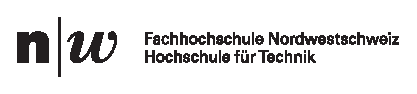
\includegraphics[height=12mm]{images/titlepage/fhnw.eps}%
        };
    \end{tikzpicture}



    % ---------------------------------------------------- %
    % The Text can  be set rather low in  the page without %
    % adjusting the top lengths.                           %
    % Backing up  and reseting these lengths  seems not to %
    % be necessary;  it appears  they are restored  at the %
    % end of the titlingpage environment.                  %
    % ---------------------------------------------------- %
    \setlength{\headsep}{0pt}
    \setlength{\headheight}{0pt}
    \setlength{\uppermargin}{4em}
    \checkandfixthelayout


    % ---------------------------------------------------- %
    % By   default,  centering   inside  the   titlingpage %
    % environment  will   center  with  respects   to  the %
    % typeblock. When  the  typeblock  is  centered,  this %
    % leads to  centered text  with respect to  the entire %
    % title  page. However,  When  the  typeblock  is  not %
    % centered, some adjustment is needed.                 %
    % See memman Chapter "Titles" for more information.    %
    % ---------------------------------------------------- %
    \calccentering{\unitlength}
    \begin{adjustwidth*}{\unitlength}{-\unitlength}


    % ---------------------------------------------------- %
    % Work some  magic to  automatically adjust  the hrule %
    % lengths to the length of the book title.             %
    %                                                      %
    % NOTE: The  font  size setting  needs  to  be in  the %
    % \mytitle  command, otherwise  \settolength will  not %
    % take it  into account  and will only  calculate with %
    % the default font size.                               %
    %                                                      %
    % NOTE  2: This mechanism  breaks if  the title  spans %
    % across multiple  lines. You're on  your own  in that %
    % case.                                                %
    % ---------------------------------------------------- %
    %\newcommand{\mytitle}{{\textbf{\fontsize{25mm}{1em}\selectfont Project Powerline}}} % default font
    \newcommand{\mytitle}{{\textbf{\fontsize{12mm}{1em}\selectfont Project Powerline}}}
    \newlength{\titlelength}            % Length of title text
    \settowidth{\titlelength}{\mytitle}
    \newcommand{\titlerulefactor}{1.2}  % Length of title rules, as a factor

    % ---------------------------------------------------- %
    % Set the title color                                  %
    % ---------------------------------------------------- %
    \newcommand{\titlecolor}{black}

    % ---------------------------------------------------- %
    % Put the title onto the page                          %
    % ---------------------------------------------------- %
    \textcolor{\titlecolor}{%
        \centering
        \rule{\titlerulefactor\titlelength}{1pt} \\
        \vspace*{4mm}
        \mytitle\\
        %\vspace*{5mm}
        \rule{\titlerulefactor\titlelength}{1pt} \\
        \vspace*{6mm}
        \fontsize{8mm}{1em}\selectfont Fachbericht \\
    }


    % ---------------------------------------------------- %
    % This is the end of the centering magic.              %
    % ---------------------------------------------------- %
    \end{adjustwidth*}


    % ---------------------------------------------------- %
    % Make  sure  this  is   not  put  into  \frontmatter, %
    % otherwise it will get a \frontmatter folio.          %
    % \cleardoblepage  is not  actually necessary  because %
    % it  is  automatically   called  by  the  titlingpage %
    % environment.                                         %
    % ---------------------------------------------------- %
    %\cleardoublepage

    %\setlength{\headsep}{\originallength}
    %\checkandfixthelayout
\end{titlingpage}


% -------------------------------------------------------- %
% See  the  memoir  documentation  for  what  specifically %
% frontmatter does. Among  other things, page  numbers are %
% set to roman numerals and chapter numbers are removed.   %
% -------------------------------------------------------- %
\frontmatter

% -------------------------------------------------------- %
% Comment out what's not needed, obviously.                %
% -------------------------------------------------------- %
%\begin{centering}
\vspace*{30mm}
\begin{tiny}
    \begin{tabular}{lll}
        Inhalt & \copyright~2016 & Marcel Heymann    \\
               &                 & Noah Hüsser       \\
               &                 & Raphael Frey      \\
               &                 & Dominik Keller    \\
               &                 & Marco Koch        \\
               &                 & Reto Nussbaumer   \\
               &                 & Francesco Rovelli \\
               &                 &                   \\
        Design & \copyright~2016 & Raphael Frey      \\
    \end{tabular}


    % ---------------------------------------------------- %
    % Having  this  in  a  tabular  is  a  bit  ugly,  but %
    % it  ensures alignment  and  limited paragraph  width %
    % without much effort.                                 %
    % ---------------------------------------------------- %
    \vspace{1em}
    \begin{tabular}{p{.9\textwidth}}
        \noindent  Erstellt  im  Fr\"uhlingssemester 2016  an  der  Hochschule
        f\"ur  Technik  der  Fachhochschule   Nordwestschweiz  im  Rahmen  des
        Modules   \emph{Projekt  4}   des   Studiengangs  \emph{Elektro-   und
        Informationstechnologie}. \\

        \\
        \iftoggle{paper}{%
            Dies     ist    die     Druckversion    dieses     Dokuments. Eine
            elektronische     Version      mit     farbig     hervorgehobenen,
            klickbaren   Links   ist   auf  den   abgegebenen   elektronischen
            Datentr\"agern  in  Anhang \ref{app:electronicStorage}  auf  Seite
            \pageref{app:electronicStorage}   zu   finden    oder   kann   bei
            \code{raphael.frey@students.fhnw.ch} angefordert werden.
        }{%
            Dies ist die elektronische  Ausf\"uhrung des Dokuments. Links sind
            farbig hervorgehoben und klickbar. Falls eine Version ohne farbige
            Akzentuierung erw\"unscht ist, kann diese bei
            \href{mailto:raphael.frey@students.fhnw.ch}{\code{raphael.frey@students.fhnw.ch}}
            angefordert werden.
            % internet links: blau
            % externe links: magenta
        }
        \\

        \\
        Dieses Dokument hat bisher \thecounttexruns~Kompiliervorg\"ange durchlaufen. \\
    \end{tabular}
    \vspace{1em}

    \begin{tabular}{>{\ttfamily}lrl}
        Version 0.1 & 06.05.2016 & Einleitung, Disposition \\
    \end{tabular}

    \vspace{1em}
    \begin{tabular}{l @{${}:{}$} l}
        Quelle Titelbild & \cite{ref:titlepage:pvanlage} \\
        Quelle Logo FHNW & \cite{ref:fhnwlogo}           \\
    \end{tabular}
\end{tiny}
%\\
%\footnotesize{\checkmark~\np~\noi~\partially} \\
%\\
%\large{\checkmark~\np~\noi~\partially} \\
%\\
%\checkmark~\np~\noi~\partially
%\end{centering}

% **************************************************************************** %
\chapter*{Abstract}
\label{chap:abstract}
% **************************************************************************** %
\enlargethispage{2em}

This project's  aim was to develop  a system for real-time  monitoring of each
panel  of a  photovoltaic facility.   The  system must  be cost-effective  and
should scale  from small single-household solutions  to large industrial-scale
solar  farms. Panels which  are not  operating at  full capacity  for whatever
reason (dirt, shade,  defects) must be detected and the  user informed so that
appropriate measures (cleaning, replacement) can be taken.

Monitoring  of  the  individual  photovoltaic modules  allows  the  facility's
operator to  optimally run  their solar  plant, thus  reducing losses  in both
power output and profit.

Current solutions for per-module monitoring  of solar facilities are expensive
and often left  out to save costs.   As alternative sources of  energy such as
wind and  solar power  grow in  importance, the overall  losses in  the energy
industry of power  and money incurred due to insufficient  monitoring of solar
facilities will become unsustainable.

Our  system  has  two  primary components: A  controller  which  is  installed
centrally  near  the  inverter  and  a  sensor  on  each  photovoltaic  panel.
Communication between the sensors and the  master is routed through the direct
current power  transmission line;  no additional wiring  is needed. A  coil is
used to couple the signal to the power line. In case of an error (e.g. a dirty
panel), an error message is sent to a user-configurable phone number.

Simulations for  various coupling methods  for a string  of 20 PV  panels have
been performed. Inductive  coupling at  non-resonance conditions results  in a
signal  level  of roughly  \SI{6}{\milli\volt}  peak-to-peak  at the  receiver
without  amplification. Operating  the  circuit  at resonance  yields  a  much
improved peak-to-peak  voltage of \SI{250}{\milli\volt} at  the receiver (also
without amplification), which is sufficient for our purposes.

A  frequency sweep  for  the coupling  coil has  been  measured and  inductive
behavior up to  \SI{20}{\mega\hertz} verified, thus ensuring that  the coil is
adaptable enough to allow the use of a vast range of frequencies as needed.

The system's components have been implemented. A  signal can be coupled to the
DC transmission line  and the sensor can perform  correct voltage measurements
and return that  data. Both the graphical user interface on  the master device
and its database back-end are functioning.

\vspace{2em}
\textbf{Key  words:}  photovoltaic  technology,  photovoltaic  module,  remote
monitoring, solar technology, PV cell, power efficiency, alternative energy,
powerline, communication, inductive coupling, capacitive coupling

%\include{frontmatter/dedication}
%\include{frontmatter/declaration}
%\include{frontmatter/acknowledgements}


% -------------------------------------------------------- %
% The starred versions do not make an entry for themselves %
% in the ToC, the unstarred versions do.                   %
% -------------------------------------------------------- %
\tableofcontents*
%\listoffigures
%\listoftables


% -------------------------------------------------------- %
% Set page numbers to  arabic numerals, reset page counter %
% to 1, display  chapter numbers. See memoir documentation %
% for more information.                                    %
% -------------------------------------------------------- %
\mainmatter


% -------------------------------------------------------- %
% It is  advisable to use actually  meaningful chapter and %
% section names instead of generically numbered ones as in %
% this  example structure. That  way, their  place in  the %
% document is not directly tied to their file name, and it %
% is  possible to  restructure the  document (e.g.  move a %
% section  from one  chapter  to another,  or reorder  the %
% chapters)  without  needing  to adjust  file  names  and %
% similar shenanigans.                                     %
% -------------------------------------------------------- %
% **************************************************************************** %
\chapter{Einleitung}
\label{chap:einleitung}
% **************************************************************************** %

Photovoltaikanlagen   sind  heutzutage   kein   Nischenprodukt  mehr. Um   die
Abhängigkeit  vom Erdöl  zu verringern,  werden vielerorts  kleine, aber  auch
grosse  Anlagen gebaut. Die  W\"arme-Energie, welche  kostenlos von  der Sonne
kommt,  wird  in elektrische  Energie  umgewandelt  und  kann gleich  vor  Ort
genutzt werden. Anlagenbesitzer  investieren meistens einen grossen  Betrag in
eine  neue  Anlage  und  sind  darauf angewiesen,  dass  diese  den  maximalen
Ertrag  liefert. Das ist  in der  Regel  ohne grossen  Aufwand der  Fall. Doch
es  gibt Umstände,  welche  die Effizienz  einer Photovoltaikanlage  erheblich
verringern  können und  dies meist  ohne, dass  es jemand  bemerkt.  In  einer
Photovoltaikanlage  werden üblicherweise  mehrere  PV-Module  zu einem  String
zusammengefasst,  indem  sie  in   Serie  geschaltet  werden. Dabei  kann  ein
abgeschattetes,  verschmutztes  oder  gar  defektes  Modul  den  Strom  dieser
Serieschaltung und somit auch die Leistung des gesamten Strings und der Anlage
stark beeinträchtigen. Was grosse finanzielle Einbussen zur Folge haben kann.

Das  Ziel des  Projektes P4  war es,  ein PV-Überwachungssystem  bestehend aus
einer Sensorplatine für den Einbau in  die Anschlussbox jedes Moduls und einem
zentralen Meldegerät  für den Einbau  im Schaltschrank beim  Wechselrichter zu
entwickeln, aufzubauen und zu testen. Die  Sensorplatine soll die Spannung des
jeweiligen PV-Modules  messen und sie  an das Mastergerät über  die bestehende
DC-Leitung  der  Anlage  übermitteln. Im  Mastergerät  werden  die  gemessenen
Spannungen der  einzelnen PV-Module  gespeichert und  ausgewertet. Erkennt das
Mastergerät ein fehlerhaftes  PV-Modul, soll eine Alarmierung  am Gerät selbst
und  per  SMS  ausgegeben  werden. Zusätzlich wird  ein  Relais  zur  externen
Signalisation  betätigt.   Das  System  soll  möglichst  energieeffizient  und
kostengünstig sein,  um die wirtschaftlichkeit einer  Photovoltaikanlage nicht
zu verschlechtern.

Das  Hauptproblem liegt  bei  der Signalübertragung  über  die DC-Leitung  der
Photovoltaikanlage. Denn die Spannung darauf schwankt  zwischen 12 und 60 Volt
an der Sensorplatine  und beträgt am Mastergerät bis zu  1000 Volt. Auf dieser
Leitung  ein Signal  zu  übertragen  ist schwierig  und  wird heutzutage  kaum
gemacht.  Zudem muss auf kleine Leistung beim gesamten System geachtet werden,
um keine wertfolle Energie zu verschwenden.

\todo{Beschreibung unseres Produkts}

Der vorliegende  Bericht stellt  die technische Dokumentation  unseres Systems
dar.  Zuerst wird das Konzept unserer L\"osung beschrieben, zusammen mit einer
Benutzerf\"uhrung.  Anschliessend  wird auf  das Hardware-  und Firmwaredesign
eingegangen,  und   zuletzt  werden  die  am   System  durchgef\"uhrten  Tests
dokumentiert.

% **************************************************************************** %
\chapter{\"Uberblick}
\label{chap:uberblick}
% **************************************************************************** %
Dieses Kapitel  beschreibt zuerst die grobe  Idee unsers L\"osungskonzepts. Es
wird  dargelegt, wie  unser System  in  eine Solaranlage  (bestehend oder  neu
aufgebaut) integriert wird, wie das System mit seiner Umgebung interagiert und
wie es zu bedienen ist.


% ---------------------------------------------------------------------------- %
\section{Aufbau einer Solaranlage}
\label{sec:solaranlage:aufbau}
% ---------------------------------------------------------------------------- %

Grunds\"atzlicher Aufbau einer Solaranlage: Zelle -> Modul -> Strings -> Anlage


% ---------------------------------------------------------------------------- %
\section{Einbettung in Umwelt}
\label{sec:einbettung}
% ---------------------------------------------------------------------------- %

Hier  wird  beschrieben,  wie  unser System  physisch  mit  einer  Solaranlage
integriert wird und welche Schnittstellen es zu welchem Zweck zur Anlage hat.
\todo{kein eigener Abschnitt mehr n\"otig}


% ---------------------------------------------------------------------------- %
\section{Kernproblem: Kommunikation \"uber DC-Leitung}
\label{sec:commDCLine}
% ---------------------------------------------------------------------------- %

\todo{Referenz auf Konzept aus obigem Kapitel}
Es sind  zwei L\"osungsans\"atze untersucht  worden, um ein Signal  \"uber die
Gleichstromleitung zu senden:

\textbf{Frequency-shift keying}: Bei  der FSK (Frequenzumtastung  auf Deutsch)
wird  dem in  der Leitung  fliessenden Gleichstrom  ein (verh\"altnism\"assig)
kleines  Signal aufmoduliert,  welches  die  zu \"ubertragenden  Informationen
enth\"alt. Die  Frequenz   des  aufmodulierten   Anteils  wird   in  diskreten
Schritten variiert  und jeweils  einem Symbol zugeordnet. Bei  einer bin\"aren
Umsetzung  werden  zwei  Frequenzen  benutzt; eine  f\"ur  \code{0}  und  eine
f\"ur  \code{1}.   Das  Verfahren ist  schematisch  in  \fref{fig:fsk:concept}
dargestellt.

\begin{figure}[h!tb]
    \centering
    %% Creator: Matplotlib, PGF backend
%%
%% To include the figure in your LaTeX document, write
%%   \input{<filename>.pgf}
%%
%% Make sure the required packages are loaded in your preamble
%%   \usepackage{pgf}
%%
%% Figures using additional raster images can only be included by \input if
%% they are in the same directory as the main LaTeX file. For loading figures
%% from other directories you can use the `import` package
%%   \usepackage{import}
%% and then include the figures with
%%   \import{<path to file>}{<filename>.pgf}
%%
%% Matplotlib used the following preamble
%%   \usepackage{fontspec}
%%   \setmainfont{Bitstream Vera Serif}
%%   \setsansfont{Bitstream Vera Sans}
%%   \setmonofont{Bitstream Vera Sans Mono}
%%
\begingroup%
\makeatletter%
\begin{pgfpicture}%
\pgfpathrectangle{\pgfpointorigin}{\pgfqpoint{4.500000in}{3.500000in}}%
\pgfusepath{use as bounding box, clip}%
\begin{pgfscope}%
\pgfsetbuttcap%
\pgfsetmiterjoin%
\pgfsetlinewidth{0.000000pt}%
\definecolor{currentstroke}{rgb}{0.000000,0.000000,0.000000}%
\pgfsetstrokecolor{currentstroke}%
\pgfsetstrokeopacity{0.000000}%
\pgfsetdash{}{0pt}%
\pgfpathmoveto{\pgfqpoint{0.000000in}{0.000000in}}%
\pgfpathlineto{\pgfqpoint{4.500000in}{0.000000in}}%
\pgfpathlineto{\pgfqpoint{4.500000in}{3.500000in}}%
\pgfpathlineto{\pgfqpoint{0.000000in}{3.500000in}}%
\pgfpathclose%
\pgfusepath{}%
\end{pgfscope}%
\begin{pgfscope}%
\pgfsetbuttcap%
\pgfsetmiterjoin%
\pgfsetlinewidth{0.000000pt}%
\definecolor{currentstroke}{rgb}{0.000000,0.000000,0.000000}%
\pgfsetstrokecolor{currentstroke}%
\pgfsetstrokeopacity{0.000000}%
\pgfsetdash{}{0pt}%
\pgfpathmoveto{\pgfqpoint{0.675000in}{2.268396in}}%
\pgfpathlineto{\pgfqpoint{4.275000in}{2.268396in}}%
\pgfpathlineto{\pgfqpoint{4.275000in}{3.325000in}}%
\pgfpathlineto{\pgfqpoint{0.675000in}{3.325000in}}%
\pgfpathclose%
\pgfusepath{}%
\end{pgfscope}%
\begin{pgfscope}%
\pgfpathrectangle{\pgfqpoint{0.675000in}{2.268396in}}{\pgfqpoint{3.600000in}{1.056604in}} %
\pgfusepath{clip}%
\pgfsetrectcap%
\pgfsetroundjoin%
\pgfsetlinewidth{0.501875pt}%
\definecolor{currentstroke}{rgb}{0.000000,0.000000,1.000000}%
\pgfsetstrokecolor{currentstroke}%
\pgfsetdash{}{0pt}%
\pgfpathmoveto{\pgfqpoint{0.675000in}{2.356447in}}%
\pgfpathlineto{\pgfqpoint{1.531798in}{2.356447in}}%
\pgfusepath{stroke}%
\end{pgfscope}%
\begin{pgfscope}%
\pgfpathrectangle{\pgfqpoint{0.675000in}{2.268396in}}{\pgfqpoint{3.600000in}{1.056604in}} %
\pgfusepath{clip}%
\pgfsetrectcap%
\pgfsetroundjoin%
\pgfsetlinewidth{0.501875pt}%
\definecolor{currentstroke}{rgb}{0.501961,0.501961,0.501961}%
\pgfsetstrokecolor{currentstroke}%
\pgfsetdash{}{0pt}%
\pgfpathmoveto{\pgfqpoint{1.531798in}{2.356447in}}%
\pgfpathlineto{\pgfqpoint{1.531798in}{3.236950in}}%
\pgfusepath{stroke}%
\end{pgfscope}%
\begin{pgfscope}%
\pgfpathrectangle{\pgfqpoint{0.675000in}{2.268396in}}{\pgfqpoint{3.600000in}{1.056604in}} %
\pgfusepath{clip}%
\pgfsetrectcap%
\pgfsetroundjoin%
\pgfsetlinewidth{0.501875pt}%
\definecolor{currentstroke}{rgb}{1.000000,0.000000,1.000000}%
\pgfsetstrokecolor{currentstroke}%
\pgfsetdash{}{0pt}%
\pgfpathmoveto{\pgfqpoint{1.531798in}{3.236950in}}%
\pgfpathlineto{\pgfqpoint{2.388596in}{3.236950in}}%
\pgfusepath{stroke}%
\end{pgfscope}%
\begin{pgfscope}%
\pgfpathrectangle{\pgfqpoint{0.675000in}{2.268396in}}{\pgfqpoint{3.600000in}{1.056604in}} %
\pgfusepath{clip}%
\pgfsetrectcap%
\pgfsetroundjoin%
\pgfsetlinewidth{0.501875pt}%
\definecolor{currentstroke}{rgb}{0.501961,0.501961,0.501961}%
\pgfsetstrokecolor{currentstroke}%
\pgfsetdash{}{0pt}%
\pgfpathmoveto{\pgfqpoint{2.388596in}{3.236950in}}%
\pgfpathlineto{\pgfqpoint{2.388596in}{2.356447in}}%
\pgfusepath{stroke}%
\end{pgfscope}%
\begin{pgfscope}%
\pgfpathrectangle{\pgfqpoint{0.675000in}{2.268396in}}{\pgfqpoint{3.600000in}{1.056604in}} %
\pgfusepath{clip}%
\pgfsetrectcap%
\pgfsetroundjoin%
\pgfsetlinewidth{0.501875pt}%
\definecolor{currentstroke}{rgb}{0.000000,0.000000,1.000000}%
\pgfsetstrokecolor{currentstroke}%
\pgfsetdash{}{0pt}%
\pgfpathmoveto{\pgfqpoint{2.388596in}{2.356447in}}%
\pgfpathlineto{\pgfqpoint{3.245394in}{2.356447in}}%
\pgfusepath{stroke}%
\end{pgfscope}%
\begin{pgfscope}%
\pgfpathrectangle{\pgfqpoint{0.675000in}{2.268396in}}{\pgfqpoint{3.600000in}{1.056604in}} %
\pgfusepath{clip}%
\pgfsetrectcap%
\pgfsetroundjoin%
\pgfsetlinewidth{0.501875pt}%
\definecolor{currentstroke}{rgb}{0.501961,0.501961,0.501961}%
\pgfsetstrokecolor{currentstroke}%
\pgfsetdash{}{0pt}%
\pgfpathmoveto{\pgfqpoint{3.245394in}{2.356447in}}%
\pgfpathlineto{\pgfqpoint{3.245394in}{3.236950in}}%
\pgfusepath{stroke}%
\end{pgfscope}%
\begin{pgfscope}%
\pgfpathrectangle{\pgfqpoint{0.675000in}{2.268396in}}{\pgfqpoint{3.600000in}{1.056604in}} %
\pgfusepath{clip}%
\pgfsetrectcap%
\pgfsetroundjoin%
\pgfsetlinewidth{0.501875pt}%
\definecolor{currentstroke}{rgb}{1.000000,0.000000,1.000000}%
\pgfsetstrokecolor{currentstroke}%
\pgfsetdash{}{0pt}%
\pgfpathmoveto{\pgfqpoint{3.245394in}{3.236950in}}%
\pgfpathlineto{\pgfqpoint{4.102192in}{3.236950in}}%
\pgfusepath{stroke}%
\end{pgfscope}%
\begin{pgfscope}%
\pgfsetrectcap%
\pgfsetmiterjoin%
\pgfsetlinewidth{0.501875pt}%
\definecolor{currentstroke}{rgb}{0.000000,0.000000,0.000000}%
\pgfsetstrokecolor{currentstroke}%
\pgfsetdash{}{0pt}%
\pgfpathmoveto{\pgfqpoint{0.675000in}{3.325000in}}%
\pgfpathlineto{\pgfqpoint{4.275000in}{3.325000in}}%
\pgfusepath{stroke}%
\end{pgfscope}%
\begin{pgfscope}%
\pgfsetrectcap%
\pgfsetmiterjoin%
\pgfsetlinewidth{0.501875pt}%
\definecolor{currentstroke}{rgb}{0.000000,0.000000,0.000000}%
\pgfsetstrokecolor{currentstroke}%
\pgfsetdash{}{0pt}%
\pgfpathmoveto{\pgfqpoint{0.675000in}{2.268396in}}%
\pgfpathlineto{\pgfqpoint{0.675000in}{3.325000in}}%
\pgfusepath{stroke}%
\end{pgfscope}%
\begin{pgfscope}%
\pgfsetrectcap%
\pgfsetmiterjoin%
\pgfsetlinewidth{0.501875pt}%
\definecolor{currentstroke}{rgb}{0.000000,0.000000,0.000000}%
\pgfsetstrokecolor{currentstroke}%
\pgfsetdash{}{0pt}%
\pgfpathmoveto{\pgfqpoint{4.275000in}{2.268396in}}%
\pgfpathlineto{\pgfqpoint{4.275000in}{3.325000in}}%
\pgfusepath{stroke}%
\end{pgfscope}%
\begin{pgfscope}%
\pgfsetrectcap%
\pgfsetmiterjoin%
\pgfsetlinewidth{0.501875pt}%
\definecolor{currentstroke}{rgb}{0.000000,0.000000,0.000000}%
\pgfsetstrokecolor{currentstroke}%
\pgfsetdash{}{0pt}%
\pgfpathmoveto{\pgfqpoint{0.675000in}{2.268396in}}%
\pgfpathlineto{\pgfqpoint{4.275000in}{2.268396in}}%
\pgfusepath{stroke}%
\end{pgfscope}%
\begin{pgfscope}%
\pgfsetbuttcap%
\pgfsetroundjoin%
\definecolor{currentfill}{rgb}{0.000000,0.000000,0.000000}%
\pgfsetfillcolor{currentfill}%
\pgfsetlinewidth{0.501875pt}%
\definecolor{currentstroke}{rgb}{0.000000,0.000000,0.000000}%
\pgfsetstrokecolor{currentstroke}%
\pgfsetdash{}{0pt}%
\pgfsys@defobject{currentmarker}{\pgfqpoint{0.000000in}{0.000000in}}{\pgfqpoint{0.000000in}{0.055556in}}{%
\pgfpathmoveto{\pgfqpoint{0.000000in}{0.000000in}}%
\pgfpathlineto{\pgfqpoint{0.000000in}{0.055556in}}%
\pgfusepath{stroke,fill}%
}%
\begin{pgfscope}%
\pgfsys@transformshift{0.675000in}{2.268396in}%
\pgfsys@useobject{currentmarker}{}%
\end{pgfscope}%
\end{pgfscope}%
\begin{pgfscope}%
\pgfsetbuttcap%
\pgfsetroundjoin%
\definecolor{currentfill}{rgb}{0.000000,0.000000,0.000000}%
\pgfsetfillcolor{currentfill}%
\pgfsetlinewidth{0.501875pt}%
\definecolor{currentstroke}{rgb}{0.000000,0.000000,0.000000}%
\pgfsetstrokecolor{currentstroke}%
\pgfsetdash{}{0pt}%
\pgfsys@defobject{currentmarker}{\pgfqpoint{0.000000in}{-0.055556in}}{\pgfqpoint{0.000000in}{0.000000in}}{%
\pgfpathmoveto{\pgfqpoint{0.000000in}{0.000000in}}%
\pgfpathlineto{\pgfqpoint{0.000000in}{-0.055556in}}%
\pgfusepath{stroke,fill}%
}%
\begin{pgfscope}%
\pgfsys@transformshift{0.675000in}{3.325000in}%
\pgfsys@useobject{currentmarker}{}%
\end{pgfscope}%
\end{pgfscope}%
\begin{pgfscope}%
\pgftext[x=0.675000in,y=2.212841in,,top]{\rmfamily\fontsize{9.000000}{10.800000}\selectfont \(\displaystyle 0.0000\)}%
\end{pgfscope}%
\begin{pgfscope}%
\pgfsetbuttcap%
\pgfsetroundjoin%
\definecolor{currentfill}{rgb}{0.000000,0.000000,0.000000}%
\pgfsetfillcolor{currentfill}%
\pgfsetlinewidth{0.501875pt}%
\definecolor{currentstroke}{rgb}{0.000000,0.000000,0.000000}%
\pgfsetstrokecolor{currentstroke}%
\pgfsetdash{}{0pt}%
\pgfsys@defobject{currentmarker}{\pgfqpoint{0.000000in}{0.000000in}}{\pgfqpoint{0.000000in}{0.055556in}}{%
\pgfpathmoveto{\pgfqpoint{0.000000in}{0.000000in}}%
\pgfpathlineto{\pgfqpoint{0.000000in}{0.055556in}}%
\pgfusepath{stroke,fill}%
}%
\begin{pgfscope}%
\pgfsys@transformshift{1.125000in}{2.268396in}%
\pgfsys@useobject{currentmarker}{}%
\end{pgfscope}%
\end{pgfscope}%
\begin{pgfscope}%
\pgfsetbuttcap%
\pgfsetroundjoin%
\definecolor{currentfill}{rgb}{0.000000,0.000000,0.000000}%
\pgfsetfillcolor{currentfill}%
\pgfsetlinewidth{0.501875pt}%
\definecolor{currentstroke}{rgb}{0.000000,0.000000,0.000000}%
\pgfsetstrokecolor{currentstroke}%
\pgfsetdash{}{0pt}%
\pgfsys@defobject{currentmarker}{\pgfqpoint{0.000000in}{-0.055556in}}{\pgfqpoint{0.000000in}{0.000000in}}{%
\pgfpathmoveto{\pgfqpoint{0.000000in}{0.000000in}}%
\pgfpathlineto{\pgfqpoint{0.000000in}{-0.055556in}}%
\pgfusepath{stroke,fill}%
}%
\begin{pgfscope}%
\pgfsys@transformshift{1.125000in}{3.325000in}%
\pgfsys@useobject{currentmarker}{}%
\end{pgfscope}%
\end{pgfscope}%
\begin{pgfscope}%
\pgftext[x=1.125000in,y=2.212841in,,top]{\rmfamily\fontsize{9.000000}{10.800000}\selectfont \(\displaystyle 0.0002\)}%
\end{pgfscope}%
\begin{pgfscope}%
\pgfsetbuttcap%
\pgfsetroundjoin%
\definecolor{currentfill}{rgb}{0.000000,0.000000,0.000000}%
\pgfsetfillcolor{currentfill}%
\pgfsetlinewidth{0.501875pt}%
\definecolor{currentstroke}{rgb}{0.000000,0.000000,0.000000}%
\pgfsetstrokecolor{currentstroke}%
\pgfsetdash{}{0pt}%
\pgfsys@defobject{currentmarker}{\pgfqpoint{0.000000in}{0.000000in}}{\pgfqpoint{0.000000in}{0.055556in}}{%
\pgfpathmoveto{\pgfqpoint{0.000000in}{0.000000in}}%
\pgfpathlineto{\pgfqpoint{0.000000in}{0.055556in}}%
\pgfusepath{stroke,fill}%
}%
\begin{pgfscope}%
\pgfsys@transformshift{1.575000in}{2.268396in}%
\pgfsys@useobject{currentmarker}{}%
\end{pgfscope}%
\end{pgfscope}%
\begin{pgfscope}%
\pgfsetbuttcap%
\pgfsetroundjoin%
\definecolor{currentfill}{rgb}{0.000000,0.000000,0.000000}%
\pgfsetfillcolor{currentfill}%
\pgfsetlinewidth{0.501875pt}%
\definecolor{currentstroke}{rgb}{0.000000,0.000000,0.000000}%
\pgfsetstrokecolor{currentstroke}%
\pgfsetdash{}{0pt}%
\pgfsys@defobject{currentmarker}{\pgfqpoint{0.000000in}{-0.055556in}}{\pgfqpoint{0.000000in}{0.000000in}}{%
\pgfpathmoveto{\pgfqpoint{0.000000in}{0.000000in}}%
\pgfpathlineto{\pgfqpoint{0.000000in}{-0.055556in}}%
\pgfusepath{stroke,fill}%
}%
\begin{pgfscope}%
\pgfsys@transformshift{1.575000in}{3.325000in}%
\pgfsys@useobject{currentmarker}{}%
\end{pgfscope}%
\end{pgfscope}%
\begin{pgfscope}%
\pgftext[x=1.575000in,y=2.212841in,,top]{\rmfamily\fontsize{9.000000}{10.800000}\selectfont \(\displaystyle 0.0004\)}%
\end{pgfscope}%
\begin{pgfscope}%
\pgfsetbuttcap%
\pgfsetroundjoin%
\definecolor{currentfill}{rgb}{0.000000,0.000000,0.000000}%
\pgfsetfillcolor{currentfill}%
\pgfsetlinewidth{0.501875pt}%
\definecolor{currentstroke}{rgb}{0.000000,0.000000,0.000000}%
\pgfsetstrokecolor{currentstroke}%
\pgfsetdash{}{0pt}%
\pgfsys@defobject{currentmarker}{\pgfqpoint{0.000000in}{0.000000in}}{\pgfqpoint{0.000000in}{0.055556in}}{%
\pgfpathmoveto{\pgfqpoint{0.000000in}{0.000000in}}%
\pgfpathlineto{\pgfqpoint{0.000000in}{0.055556in}}%
\pgfusepath{stroke,fill}%
}%
\begin{pgfscope}%
\pgfsys@transformshift{2.025000in}{2.268396in}%
\pgfsys@useobject{currentmarker}{}%
\end{pgfscope}%
\end{pgfscope}%
\begin{pgfscope}%
\pgfsetbuttcap%
\pgfsetroundjoin%
\definecolor{currentfill}{rgb}{0.000000,0.000000,0.000000}%
\pgfsetfillcolor{currentfill}%
\pgfsetlinewidth{0.501875pt}%
\definecolor{currentstroke}{rgb}{0.000000,0.000000,0.000000}%
\pgfsetstrokecolor{currentstroke}%
\pgfsetdash{}{0pt}%
\pgfsys@defobject{currentmarker}{\pgfqpoint{0.000000in}{-0.055556in}}{\pgfqpoint{0.000000in}{0.000000in}}{%
\pgfpathmoveto{\pgfqpoint{0.000000in}{0.000000in}}%
\pgfpathlineto{\pgfqpoint{0.000000in}{-0.055556in}}%
\pgfusepath{stroke,fill}%
}%
\begin{pgfscope}%
\pgfsys@transformshift{2.025000in}{3.325000in}%
\pgfsys@useobject{currentmarker}{}%
\end{pgfscope}%
\end{pgfscope}%
\begin{pgfscope}%
\pgftext[x=2.025000in,y=2.212841in,,top]{\rmfamily\fontsize{9.000000}{10.800000}\selectfont \(\displaystyle 0.0006\)}%
\end{pgfscope}%
\begin{pgfscope}%
\pgfsetbuttcap%
\pgfsetroundjoin%
\definecolor{currentfill}{rgb}{0.000000,0.000000,0.000000}%
\pgfsetfillcolor{currentfill}%
\pgfsetlinewidth{0.501875pt}%
\definecolor{currentstroke}{rgb}{0.000000,0.000000,0.000000}%
\pgfsetstrokecolor{currentstroke}%
\pgfsetdash{}{0pt}%
\pgfsys@defobject{currentmarker}{\pgfqpoint{0.000000in}{0.000000in}}{\pgfqpoint{0.000000in}{0.055556in}}{%
\pgfpathmoveto{\pgfqpoint{0.000000in}{0.000000in}}%
\pgfpathlineto{\pgfqpoint{0.000000in}{0.055556in}}%
\pgfusepath{stroke,fill}%
}%
\begin{pgfscope}%
\pgfsys@transformshift{2.475000in}{2.268396in}%
\pgfsys@useobject{currentmarker}{}%
\end{pgfscope}%
\end{pgfscope}%
\begin{pgfscope}%
\pgfsetbuttcap%
\pgfsetroundjoin%
\definecolor{currentfill}{rgb}{0.000000,0.000000,0.000000}%
\pgfsetfillcolor{currentfill}%
\pgfsetlinewidth{0.501875pt}%
\definecolor{currentstroke}{rgb}{0.000000,0.000000,0.000000}%
\pgfsetstrokecolor{currentstroke}%
\pgfsetdash{}{0pt}%
\pgfsys@defobject{currentmarker}{\pgfqpoint{0.000000in}{-0.055556in}}{\pgfqpoint{0.000000in}{0.000000in}}{%
\pgfpathmoveto{\pgfqpoint{0.000000in}{0.000000in}}%
\pgfpathlineto{\pgfqpoint{0.000000in}{-0.055556in}}%
\pgfusepath{stroke,fill}%
}%
\begin{pgfscope}%
\pgfsys@transformshift{2.475000in}{3.325000in}%
\pgfsys@useobject{currentmarker}{}%
\end{pgfscope}%
\end{pgfscope}%
\begin{pgfscope}%
\pgftext[x=2.475000in,y=2.212841in,,top]{\rmfamily\fontsize{9.000000}{10.800000}\selectfont \(\displaystyle 0.0008\)}%
\end{pgfscope}%
\begin{pgfscope}%
\pgfsetbuttcap%
\pgfsetroundjoin%
\definecolor{currentfill}{rgb}{0.000000,0.000000,0.000000}%
\pgfsetfillcolor{currentfill}%
\pgfsetlinewidth{0.501875pt}%
\definecolor{currentstroke}{rgb}{0.000000,0.000000,0.000000}%
\pgfsetstrokecolor{currentstroke}%
\pgfsetdash{}{0pt}%
\pgfsys@defobject{currentmarker}{\pgfqpoint{0.000000in}{0.000000in}}{\pgfqpoint{0.000000in}{0.055556in}}{%
\pgfpathmoveto{\pgfqpoint{0.000000in}{0.000000in}}%
\pgfpathlineto{\pgfqpoint{0.000000in}{0.055556in}}%
\pgfusepath{stroke,fill}%
}%
\begin{pgfscope}%
\pgfsys@transformshift{2.925000in}{2.268396in}%
\pgfsys@useobject{currentmarker}{}%
\end{pgfscope}%
\end{pgfscope}%
\begin{pgfscope}%
\pgfsetbuttcap%
\pgfsetroundjoin%
\definecolor{currentfill}{rgb}{0.000000,0.000000,0.000000}%
\pgfsetfillcolor{currentfill}%
\pgfsetlinewidth{0.501875pt}%
\definecolor{currentstroke}{rgb}{0.000000,0.000000,0.000000}%
\pgfsetstrokecolor{currentstroke}%
\pgfsetdash{}{0pt}%
\pgfsys@defobject{currentmarker}{\pgfqpoint{0.000000in}{-0.055556in}}{\pgfqpoint{0.000000in}{0.000000in}}{%
\pgfpathmoveto{\pgfqpoint{0.000000in}{0.000000in}}%
\pgfpathlineto{\pgfqpoint{0.000000in}{-0.055556in}}%
\pgfusepath{stroke,fill}%
}%
\begin{pgfscope}%
\pgfsys@transformshift{2.925000in}{3.325000in}%
\pgfsys@useobject{currentmarker}{}%
\end{pgfscope}%
\end{pgfscope}%
\begin{pgfscope}%
\pgftext[x=2.925000in,y=2.212841in,,top]{\rmfamily\fontsize{9.000000}{10.800000}\selectfont \(\displaystyle 0.0010\)}%
\end{pgfscope}%
\begin{pgfscope}%
\pgfsetbuttcap%
\pgfsetroundjoin%
\definecolor{currentfill}{rgb}{0.000000,0.000000,0.000000}%
\pgfsetfillcolor{currentfill}%
\pgfsetlinewidth{0.501875pt}%
\definecolor{currentstroke}{rgb}{0.000000,0.000000,0.000000}%
\pgfsetstrokecolor{currentstroke}%
\pgfsetdash{}{0pt}%
\pgfsys@defobject{currentmarker}{\pgfqpoint{0.000000in}{0.000000in}}{\pgfqpoint{0.000000in}{0.055556in}}{%
\pgfpathmoveto{\pgfqpoint{0.000000in}{0.000000in}}%
\pgfpathlineto{\pgfqpoint{0.000000in}{0.055556in}}%
\pgfusepath{stroke,fill}%
}%
\begin{pgfscope}%
\pgfsys@transformshift{3.375000in}{2.268396in}%
\pgfsys@useobject{currentmarker}{}%
\end{pgfscope}%
\end{pgfscope}%
\begin{pgfscope}%
\pgfsetbuttcap%
\pgfsetroundjoin%
\definecolor{currentfill}{rgb}{0.000000,0.000000,0.000000}%
\pgfsetfillcolor{currentfill}%
\pgfsetlinewidth{0.501875pt}%
\definecolor{currentstroke}{rgb}{0.000000,0.000000,0.000000}%
\pgfsetstrokecolor{currentstroke}%
\pgfsetdash{}{0pt}%
\pgfsys@defobject{currentmarker}{\pgfqpoint{0.000000in}{-0.055556in}}{\pgfqpoint{0.000000in}{0.000000in}}{%
\pgfpathmoveto{\pgfqpoint{0.000000in}{0.000000in}}%
\pgfpathlineto{\pgfqpoint{0.000000in}{-0.055556in}}%
\pgfusepath{stroke,fill}%
}%
\begin{pgfscope}%
\pgfsys@transformshift{3.375000in}{3.325000in}%
\pgfsys@useobject{currentmarker}{}%
\end{pgfscope}%
\end{pgfscope}%
\begin{pgfscope}%
\pgftext[x=3.375000in,y=2.212841in,,top]{\rmfamily\fontsize{9.000000}{10.800000}\selectfont \(\displaystyle 0.0012\)}%
\end{pgfscope}%
\begin{pgfscope}%
\pgfsetbuttcap%
\pgfsetroundjoin%
\definecolor{currentfill}{rgb}{0.000000,0.000000,0.000000}%
\pgfsetfillcolor{currentfill}%
\pgfsetlinewidth{0.501875pt}%
\definecolor{currentstroke}{rgb}{0.000000,0.000000,0.000000}%
\pgfsetstrokecolor{currentstroke}%
\pgfsetdash{}{0pt}%
\pgfsys@defobject{currentmarker}{\pgfqpoint{0.000000in}{0.000000in}}{\pgfqpoint{0.000000in}{0.055556in}}{%
\pgfpathmoveto{\pgfqpoint{0.000000in}{0.000000in}}%
\pgfpathlineto{\pgfqpoint{0.000000in}{0.055556in}}%
\pgfusepath{stroke,fill}%
}%
\begin{pgfscope}%
\pgfsys@transformshift{3.825000in}{2.268396in}%
\pgfsys@useobject{currentmarker}{}%
\end{pgfscope}%
\end{pgfscope}%
\begin{pgfscope}%
\pgfsetbuttcap%
\pgfsetroundjoin%
\definecolor{currentfill}{rgb}{0.000000,0.000000,0.000000}%
\pgfsetfillcolor{currentfill}%
\pgfsetlinewidth{0.501875pt}%
\definecolor{currentstroke}{rgb}{0.000000,0.000000,0.000000}%
\pgfsetstrokecolor{currentstroke}%
\pgfsetdash{}{0pt}%
\pgfsys@defobject{currentmarker}{\pgfqpoint{0.000000in}{-0.055556in}}{\pgfqpoint{0.000000in}{0.000000in}}{%
\pgfpathmoveto{\pgfqpoint{0.000000in}{0.000000in}}%
\pgfpathlineto{\pgfqpoint{0.000000in}{-0.055556in}}%
\pgfusepath{stroke,fill}%
}%
\begin{pgfscope}%
\pgfsys@transformshift{3.825000in}{3.325000in}%
\pgfsys@useobject{currentmarker}{}%
\end{pgfscope}%
\end{pgfscope}%
\begin{pgfscope}%
\pgftext[x=3.825000in,y=2.212841in,,top]{\rmfamily\fontsize{9.000000}{10.800000}\selectfont \(\displaystyle 0.0014\)}%
\end{pgfscope}%
\begin{pgfscope}%
\pgfsetbuttcap%
\pgfsetroundjoin%
\definecolor{currentfill}{rgb}{0.000000,0.000000,0.000000}%
\pgfsetfillcolor{currentfill}%
\pgfsetlinewidth{0.501875pt}%
\definecolor{currentstroke}{rgb}{0.000000,0.000000,0.000000}%
\pgfsetstrokecolor{currentstroke}%
\pgfsetdash{}{0pt}%
\pgfsys@defobject{currentmarker}{\pgfqpoint{0.000000in}{0.000000in}}{\pgfqpoint{0.000000in}{0.055556in}}{%
\pgfpathmoveto{\pgfqpoint{0.000000in}{0.000000in}}%
\pgfpathlineto{\pgfqpoint{0.000000in}{0.055556in}}%
\pgfusepath{stroke,fill}%
}%
\begin{pgfscope}%
\pgfsys@transformshift{4.275000in}{2.268396in}%
\pgfsys@useobject{currentmarker}{}%
\end{pgfscope}%
\end{pgfscope}%
\begin{pgfscope}%
\pgfsetbuttcap%
\pgfsetroundjoin%
\definecolor{currentfill}{rgb}{0.000000,0.000000,0.000000}%
\pgfsetfillcolor{currentfill}%
\pgfsetlinewidth{0.501875pt}%
\definecolor{currentstroke}{rgb}{0.000000,0.000000,0.000000}%
\pgfsetstrokecolor{currentstroke}%
\pgfsetdash{}{0pt}%
\pgfsys@defobject{currentmarker}{\pgfqpoint{0.000000in}{-0.055556in}}{\pgfqpoint{0.000000in}{0.000000in}}{%
\pgfpathmoveto{\pgfqpoint{0.000000in}{0.000000in}}%
\pgfpathlineto{\pgfqpoint{0.000000in}{-0.055556in}}%
\pgfusepath{stroke,fill}%
}%
\begin{pgfscope}%
\pgfsys@transformshift{4.275000in}{3.325000in}%
\pgfsys@useobject{currentmarker}{}%
\end{pgfscope}%
\end{pgfscope}%
\begin{pgfscope}%
\pgftext[x=4.275000in,y=2.212841in,,top]{\rmfamily\fontsize{9.000000}{10.800000}\selectfont \(\displaystyle 0.0016\)}%
\end{pgfscope}%
\begin{pgfscope}%
\pgftext[x=2.475000in,y=2.022425in,,top]{\rmfamily\fontsize{9.000000}{10.800000}\selectfont Zeit (s)}%
\end{pgfscope}%
\begin{pgfscope}%
\pgfsetbuttcap%
\pgfsetroundjoin%
\definecolor{currentfill}{rgb}{0.000000,0.000000,0.000000}%
\pgfsetfillcolor{currentfill}%
\pgfsetlinewidth{0.501875pt}%
\definecolor{currentstroke}{rgb}{0.000000,0.000000,0.000000}%
\pgfsetstrokecolor{currentstroke}%
\pgfsetdash{}{0pt}%
\pgfsys@defobject{currentmarker}{\pgfqpoint{0.000000in}{0.000000in}}{\pgfqpoint{0.055556in}{0.000000in}}{%
\pgfpathmoveto{\pgfqpoint{0.000000in}{0.000000in}}%
\pgfpathlineto{\pgfqpoint{0.055556in}{0.000000in}}%
\pgfusepath{stroke,fill}%
}%
\begin{pgfscope}%
\pgfsys@transformshift{0.675000in}{2.356447in}%
\pgfsys@useobject{currentmarker}{}%
\end{pgfscope}%
\end{pgfscope}%
\begin{pgfscope}%
\pgfsetbuttcap%
\pgfsetroundjoin%
\definecolor{currentfill}{rgb}{0.000000,0.000000,0.000000}%
\pgfsetfillcolor{currentfill}%
\pgfsetlinewidth{0.501875pt}%
\definecolor{currentstroke}{rgb}{0.000000,0.000000,0.000000}%
\pgfsetstrokecolor{currentstroke}%
\pgfsetdash{}{0pt}%
\pgfsys@defobject{currentmarker}{\pgfqpoint{-0.055556in}{0.000000in}}{\pgfqpoint{0.000000in}{0.000000in}}{%
\pgfpathmoveto{\pgfqpoint{0.000000in}{0.000000in}}%
\pgfpathlineto{\pgfqpoint{-0.055556in}{0.000000in}}%
\pgfusepath{stroke,fill}%
}%
\begin{pgfscope}%
\pgfsys@transformshift{4.275000in}{2.356447in}%
\pgfsys@useobject{currentmarker}{}%
\end{pgfscope}%
\end{pgfscope}%
\begin{pgfscope}%
\pgftext[x=0.619444in,y=2.356447in,right,]{\rmfamily\fontsize{9.000000}{10.800000}\selectfont \(\displaystyle 0.0\)}%
\end{pgfscope}%
\begin{pgfscope}%
\pgfsetbuttcap%
\pgfsetroundjoin%
\definecolor{currentfill}{rgb}{0.000000,0.000000,0.000000}%
\pgfsetfillcolor{currentfill}%
\pgfsetlinewidth{0.501875pt}%
\definecolor{currentstroke}{rgb}{0.000000,0.000000,0.000000}%
\pgfsetstrokecolor{currentstroke}%
\pgfsetdash{}{0pt}%
\pgfsys@defobject{currentmarker}{\pgfqpoint{0.000000in}{0.000000in}}{\pgfqpoint{0.055556in}{0.000000in}}{%
\pgfpathmoveto{\pgfqpoint{0.000000in}{0.000000in}}%
\pgfpathlineto{\pgfqpoint{0.055556in}{0.000000in}}%
\pgfusepath{stroke,fill}%
}%
\begin{pgfscope}%
\pgfsys@transformshift{0.675000in}{2.532547in}%
\pgfsys@useobject{currentmarker}{}%
\end{pgfscope}%
\end{pgfscope}%
\begin{pgfscope}%
\pgfsetbuttcap%
\pgfsetroundjoin%
\definecolor{currentfill}{rgb}{0.000000,0.000000,0.000000}%
\pgfsetfillcolor{currentfill}%
\pgfsetlinewidth{0.501875pt}%
\definecolor{currentstroke}{rgb}{0.000000,0.000000,0.000000}%
\pgfsetstrokecolor{currentstroke}%
\pgfsetdash{}{0pt}%
\pgfsys@defobject{currentmarker}{\pgfqpoint{-0.055556in}{0.000000in}}{\pgfqpoint{0.000000in}{0.000000in}}{%
\pgfpathmoveto{\pgfqpoint{0.000000in}{0.000000in}}%
\pgfpathlineto{\pgfqpoint{-0.055556in}{0.000000in}}%
\pgfusepath{stroke,fill}%
}%
\begin{pgfscope}%
\pgfsys@transformshift{4.275000in}{2.532547in}%
\pgfsys@useobject{currentmarker}{}%
\end{pgfscope}%
\end{pgfscope}%
\begin{pgfscope}%
\pgftext[x=0.619444in,y=2.532547in,right,]{\rmfamily\fontsize{9.000000}{10.800000}\selectfont \(\displaystyle 0.2\)}%
\end{pgfscope}%
\begin{pgfscope}%
\pgfsetbuttcap%
\pgfsetroundjoin%
\definecolor{currentfill}{rgb}{0.000000,0.000000,0.000000}%
\pgfsetfillcolor{currentfill}%
\pgfsetlinewidth{0.501875pt}%
\definecolor{currentstroke}{rgb}{0.000000,0.000000,0.000000}%
\pgfsetstrokecolor{currentstroke}%
\pgfsetdash{}{0pt}%
\pgfsys@defobject{currentmarker}{\pgfqpoint{0.000000in}{0.000000in}}{\pgfqpoint{0.055556in}{0.000000in}}{%
\pgfpathmoveto{\pgfqpoint{0.000000in}{0.000000in}}%
\pgfpathlineto{\pgfqpoint{0.055556in}{0.000000in}}%
\pgfusepath{stroke,fill}%
}%
\begin{pgfscope}%
\pgfsys@transformshift{0.675000in}{2.708648in}%
\pgfsys@useobject{currentmarker}{}%
\end{pgfscope}%
\end{pgfscope}%
\begin{pgfscope}%
\pgfsetbuttcap%
\pgfsetroundjoin%
\definecolor{currentfill}{rgb}{0.000000,0.000000,0.000000}%
\pgfsetfillcolor{currentfill}%
\pgfsetlinewidth{0.501875pt}%
\definecolor{currentstroke}{rgb}{0.000000,0.000000,0.000000}%
\pgfsetstrokecolor{currentstroke}%
\pgfsetdash{}{0pt}%
\pgfsys@defobject{currentmarker}{\pgfqpoint{-0.055556in}{0.000000in}}{\pgfqpoint{0.000000in}{0.000000in}}{%
\pgfpathmoveto{\pgfqpoint{0.000000in}{0.000000in}}%
\pgfpathlineto{\pgfqpoint{-0.055556in}{0.000000in}}%
\pgfusepath{stroke,fill}%
}%
\begin{pgfscope}%
\pgfsys@transformshift{4.275000in}{2.708648in}%
\pgfsys@useobject{currentmarker}{}%
\end{pgfscope}%
\end{pgfscope}%
\begin{pgfscope}%
\pgftext[x=0.619444in,y=2.708648in,right,]{\rmfamily\fontsize{9.000000}{10.800000}\selectfont \(\displaystyle 0.4\)}%
\end{pgfscope}%
\begin{pgfscope}%
\pgfsetbuttcap%
\pgfsetroundjoin%
\definecolor{currentfill}{rgb}{0.000000,0.000000,0.000000}%
\pgfsetfillcolor{currentfill}%
\pgfsetlinewidth{0.501875pt}%
\definecolor{currentstroke}{rgb}{0.000000,0.000000,0.000000}%
\pgfsetstrokecolor{currentstroke}%
\pgfsetdash{}{0pt}%
\pgfsys@defobject{currentmarker}{\pgfqpoint{0.000000in}{0.000000in}}{\pgfqpoint{0.055556in}{0.000000in}}{%
\pgfpathmoveto{\pgfqpoint{0.000000in}{0.000000in}}%
\pgfpathlineto{\pgfqpoint{0.055556in}{0.000000in}}%
\pgfusepath{stroke,fill}%
}%
\begin{pgfscope}%
\pgfsys@transformshift{0.675000in}{2.884748in}%
\pgfsys@useobject{currentmarker}{}%
\end{pgfscope}%
\end{pgfscope}%
\begin{pgfscope}%
\pgfsetbuttcap%
\pgfsetroundjoin%
\definecolor{currentfill}{rgb}{0.000000,0.000000,0.000000}%
\pgfsetfillcolor{currentfill}%
\pgfsetlinewidth{0.501875pt}%
\definecolor{currentstroke}{rgb}{0.000000,0.000000,0.000000}%
\pgfsetstrokecolor{currentstroke}%
\pgfsetdash{}{0pt}%
\pgfsys@defobject{currentmarker}{\pgfqpoint{-0.055556in}{0.000000in}}{\pgfqpoint{0.000000in}{0.000000in}}{%
\pgfpathmoveto{\pgfqpoint{0.000000in}{0.000000in}}%
\pgfpathlineto{\pgfqpoint{-0.055556in}{0.000000in}}%
\pgfusepath{stroke,fill}%
}%
\begin{pgfscope}%
\pgfsys@transformshift{4.275000in}{2.884748in}%
\pgfsys@useobject{currentmarker}{}%
\end{pgfscope}%
\end{pgfscope}%
\begin{pgfscope}%
\pgftext[x=0.619444in,y=2.884748in,right,]{\rmfamily\fontsize{9.000000}{10.800000}\selectfont \(\displaystyle 0.6\)}%
\end{pgfscope}%
\begin{pgfscope}%
\pgfsetbuttcap%
\pgfsetroundjoin%
\definecolor{currentfill}{rgb}{0.000000,0.000000,0.000000}%
\pgfsetfillcolor{currentfill}%
\pgfsetlinewidth{0.501875pt}%
\definecolor{currentstroke}{rgb}{0.000000,0.000000,0.000000}%
\pgfsetstrokecolor{currentstroke}%
\pgfsetdash{}{0pt}%
\pgfsys@defobject{currentmarker}{\pgfqpoint{0.000000in}{0.000000in}}{\pgfqpoint{0.055556in}{0.000000in}}{%
\pgfpathmoveto{\pgfqpoint{0.000000in}{0.000000in}}%
\pgfpathlineto{\pgfqpoint{0.055556in}{0.000000in}}%
\pgfusepath{stroke,fill}%
}%
\begin{pgfscope}%
\pgfsys@transformshift{0.675000in}{3.060849in}%
\pgfsys@useobject{currentmarker}{}%
\end{pgfscope}%
\end{pgfscope}%
\begin{pgfscope}%
\pgfsetbuttcap%
\pgfsetroundjoin%
\definecolor{currentfill}{rgb}{0.000000,0.000000,0.000000}%
\pgfsetfillcolor{currentfill}%
\pgfsetlinewidth{0.501875pt}%
\definecolor{currentstroke}{rgb}{0.000000,0.000000,0.000000}%
\pgfsetstrokecolor{currentstroke}%
\pgfsetdash{}{0pt}%
\pgfsys@defobject{currentmarker}{\pgfqpoint{-0.055556in}{0.000000in}}{\pgfqpoint{0.000000in}{0.000000in}}{%
\pgfpathmoveto{\pgfqpoint{0.000000in}{0.000000in}}%
\pgfpathlineto{\pgfqpoint{-0.055556in}{0.000000in}}%
\pgfusepath{stroke,fill}%
}%
\begin{pgfscope}%
\pgfsys@transformshift{4.275000in}{3.060849in}%
\pgfsys@useobject{currentmarker}{}%
\end{pgfscope}%
\end{pgfscope}%
\begin{pgfscope}%
\pgftext[x=0.619444in,y=3.060849in,right,]{\rmfamily\fontsize{9.000000}{10.800000}\selectfont \(\displaystyle 0.8\)}%
\end{pgfscope}%
\begin{pgfscope}%
\pgfsetbuttcap%
\pgfsetroundjoin%
\definecolor{currentfill}{rgb}{0.000000,0.000000,0.000000}%
\pgfsetfillcolor{currentfill}%
\pgfsetlinewidth{0.501875pt}%
\definecolor{currentstroke}{rgb}{0.000000,0.000000,0.000000}%
\pgfsetstrokecolor{currentstroke}%
\pgfsetdash{}{0pt}%
\pgfsys@defobject{currentmarker}{\pgfqpoint{0.000000in}{0.000000in}}{\pgfqpoint{0.055556in}{0.000000in}}{%
\pgfpathmoveto{\pgfqpoint{0.000000in}{0.000000in}}%
\pgfpathlineto{\pgfqpoint{0.055556in}{0.000000in}}%
\pgfusepath{stroke,fill}%
}%
\begin{pgfscope}%
\pgfsys@transformshift{0.675000in}{3.236950in}%
\pgfsys@useobject{currentmarker}{}%
\end{pgfscope}%
\end{pgfscope}%
\begin{pgfscope}%
\pgfsetbuttcap%
\pgfsetroundjoin%
\definecolor{currentfill}{rgb}{0.000000,0.000000,0.000000}%
\pgfsetfillcolor{currentfill}%
\pgfsetlinewidth{0.501875pt}%
\definecolor{currentstroke}{rgb}{0.000000,0.000000,0.000000}%
\pgfsetstrokecolor{currentstroke}%
\pgfsetdash{}{0pt}%
\pgfsys@defobject{currentmarker}{\pgfqpoint{-0.055556in}{0.000000in}}{\pgfqpoint{0.000000in}{0.000000in}}{%
\pgfpathmoveto{\pgfqpoint{0.000000in}{0.000000in}}%
\pgfpathlineto{\pgfqpoint{-0.055556in}{0.000000in}}%
\pgfusepath{stroke,fill}%
}%
\begin{pgfscope}%
\pgfsys@transformshift{4.275000in}{3.236950in}%
\pgfsys@useobject{currentmarker}{}%
\end{pgfscope}%
\end{pgfscope}%
\begin{pgfscope}%
\pgftext[x=0.619444in,y=3.236950in,right,]{\rmfamily\fontsize{9.000000}{10.800000}\selectfont \(\displaystyle 1.0\)}%
\end{pgfscope}%
\begin{pgfscope}%
\pgftext[x=0.385842in,y=2.796698in,,bottom,rotate=90.000000]{\rmfamily\fontsize{9.000000}{10.800000}\selectfont Symbol}%
\end{pgfscope}%
\begin{pgfscope}%
\pgftext[x=2.475000in,y=3.394444in,,base]{\rmfamily\fontsize{11.000000}{13.200000}\selectfont Daten}%
\end{pgfscope}%
\begin{pgfscope}%
\pgfsetbuttcap%
\pgfsetmiterjoin%
\pgfsetlinewidth{0.000000pt}%
\definecolor{currentstroke}{rgb}{0.000000,0.000000,0.000000}%
\pgfsetstrokecolor{currentstroke}%
\pgfsetstrokeopacity{0.000000}%
\pgfsetdash{}{0pt}%
\pgfpathmoveto{\pgfqpoint{0.675000in}{0.525000in}}%
\pgfpathlineto{\pgfqpoint{4.275000in}{0.525000in}}%
\pgfpathlineto{\pgfqpoint{4.275000in}{1.581604in}}%
\pgfpathlineto{\pgfqpoint{0.675000in}{1.581604in}}%
\pgfpathclose%
\pgfusepath{}%
\end{pgfscope}%
\begin{pgfscope}%
\pgfpathrectangle{\pgfqpoint{0.675000in}{0.525000in}}{\pgfqpoint{3.600000in}{1.056604in}} %
\pgfusepath{clip}%
\pgfsetrectcap%
\pgfsetroundjoin%
\pgfsetlinewidth{0.501875pt}%
\definecolor{currentstroke}{rgb}{0.000000,0.000000,1.000000}%
\pgfsetstrokecolor{currentstroke}%
\pgfsetdash{}{0pt}%
\pgfpathmoveto{\pgfqpoint{0.675000in}{0.573027in}}%
\pgfpathlineto{\pgfqpoint{0.679288in}{0.573977in}}%
\pgfpathlineto{\pgfqpoint{0.684434in}{0.577618in}}%
\pgfpathlineto{\pgfqpoint{0.690438in}{0.585286in}}%
\pgfpathlineto{\pgfqpoint{0.697299in}{0.598485in}}%
\pgfpathlineto{\pgfqpoint{0.705018in}{0.618827in}}%
\pgfpathlineto{\pgfqpoint{0.713595in}{0.647938in}}%
\pgfpathlineto{\pgfqpoint{0.723886in}{0.691280in}}%
\pgfpathlineto{\pgfqpoint{0.735894in}{0.752172in}}%
\pgfpathlineto{\pgfqpoint{0.750474in}{0.838430in}}%
\pgfpathlineto{\pgfqpoint{0.770200in}{0.969903in}}%
\pgfpathlineto{\pgfqpoint{0.818228in}{1.296050in}}%
\pgfpathlineto{\pgfqpoint{0.833666in}{1.382886in}}%
\pgfpathlineto{\pgfqpoint{0.845673in}{1.438992in}}%
\pgfpathlineto{\pgfqpoint{0.855965in}{1.477642in}}%
\pgfpathlineto{\pgfqpoint{0.865400in}{1.504612in}}%
\pgfpathlineto{\pgfqpoint{0.873118in}{1.520280in}}%
\pgfpathlineto{\pgfqpoint{0.879980in}{1.529192in}}%
\pgfpathlineto{\pgfqpoint{0.885126in}{1.532719in}}%
\pgfpathlineto{\pgfqpoint{0.890272in}{1.533517in}}%
\pgfpathlineto{\pgfqpoint{0.894560in}{1.532093in}}%
\pgfpathlineto{\pgfqpoint{0.899706in}{1.527886in}}%
\pgfpathlineto{\pgfqpoint{0.905709in}{1.519565in}}%
\pgfpathlineto{\pgfqpoint{0.912571in}{1.505636in}}%
\pgfpathlineto{\pgfqpoint{0.920290in}{1.484505in}}%
\pgfpathlineto{\pgfqpoint{0.929724in}{1.451214in}}%
\pgfpathlineto{\pgfqpoint{0.940016in}{1.406247in}}%
\pgfpathlineto{\pgfqpoint{0.952023in}{1.343724in}}%
\pgfpathlineto{\pgfqpoint{0.967461in}{1.250439in}}%
\pgfpathlineto{\pgfqpoint{0.988902in}{1.105306in}}%
\pgfpathlineto{\pgfqpoint{1.029212in}{0.830364in}}%
\pgfpathlineto{\pgfqpoint{1.045507in}{0.735997in}}%
\pgfpathlineto{\pgfqpoint{1.058372in}{0.674005in}}%
\pgfpathlineto{\pgfqpoint{1.069522in}{0.631102in}}%
\pgfpathlineto{\pgfqpoint{1.078956in}{0.603561in}}%
\pgfpathlineto{\pgfqpoint{1.086675in}{0.587403in}}%
\pgfpathlineto{\pgfqpoint{1.093536in}{0.578044in}}%
\pgfpathlineto{\pgfqpoint{1.098682in}{0.574176in}}%
\pgfpathlineto{\pgfqpoint{1.103828in}{0.573037in}}%
\pgfpathlineto{\pgfqpoint{1.108116in}{0.574176in}}%
\pgfpathlineto{\pgfqpoint{1.113262in}{0.578044in}}%
\pgfpathlineto{\pgfqpoint{1.119266in}{0.585973in}}%
\pgfpathlineto{\pgfqpoint{1.126127in}{0.599465in}}%
\pgfpathlineto{\pgfqpoint{1.133846in}{0.620123in}}%
\pgfpathlineto{\pgfqpoint{1.142422in}{0.649567in}}%
\pgfpathlineto{\pgfqpoint{1.152714in}{0.693273in}}%
\pgfpathlineto{\pgfqpoint{1.164721in}{0.754531in}}%
\pgfpathlineto{\pgfqpoint{1.179302in}{0.841136in}}%
\pgfpathlineto{\pgfqpoint{1.199028in}{0.972880in}}%
\pgfpathlineto{\pgfqpoint{1.246199in}{1.293439in}}%
\pgfpathlineto{\pgfqpoint{1.261636in}{1.380683in}}%
\pgfpathlineto{\pgfqpoint{1.273644in}{1.437184in}}%
\pgfpathlineto{\pgfqpoint{1.283936in}{1.476219in}}%
\pgfpathlineto{\pgfqpoint{1.293370in}{1.503570in}}%
\pgfpathlineto{\pgfqpoint{1.301089in}{1.519565in}}%
\pgfpathlineto{\pgfqpoint{1.307950in}{1.528775in}}%
\pgfpathlineto{\pgfqpoint{1.313096in}{1.532529in}}%
\pgfpathlineto{\pgfqpoint{1.318242in}{1.533555in}}%
\pgfpathlineto{\pgfqpoint{1.322530in}{1.532321in}}%
\pgfpathlineto{\pgfqpoint{1.327676in}{1.528340in}}%
\pgfpathlineto{\pgfqpoint{1.333680in}{1.520280in}}%
\pgfpathlineto{\pgfqpoint{1.340541in}{1.506643in}}%
\pgfpathlineto{\pgfqpoint{1.348260in}{1.485827in}}%
\pgfpathlineto{\pgfqpoint{1.356836in}{1.456217in}}%
\pgfpathlineto{\pgfqpoint{1.367128in}{1.412330in}}%
\pgfpathlineto{\pgfqpoint{1.379135in}{1.350889in}}%
\pgfpathlineto{\pgfqpoint{1.393715in}{1.264112in}}%
\pgfpathlineto{\pgfqpoint{1.413442in}{1.132235in}}%
\pgfpathlineto{\pgfqpoint{1.460613in}{0.811858in}}%
\pgfpathlineto{\pgfqpoint{1.476050in}{0.724818in}}%
\pgfpathlineto{\pgfqpoint{1.488058in}{0.668514in}}%
\pgfpathlineto{\pgfqpoint{1.498349in}{0.629671in}}%
\pgfpathlineto{\pgfqpoint{1.507784in}{0.602510in}}%
\pgfpathlineto{\pgfqpoint{1.515503in}{0.586679in}}%
\pgfpathlineto{\pgfqpoint{1.522364in}{0.577618in}}%
\pgfpathlineto{\pgfqpoint{1.527510in}{0.573977in}}%
\pgfpathlineto{\pgfqpoint{1.531798in}{0.573027in}}%
\pgfpathlineto{\pgfqpoint{1.531798in}{0.573027in}}%
\pgfusepath{stroke}%
\end{pgfscope}%
\begin{pgfscope}%
\pgfpathrectangle{\pgfqpoint{0.675000in}{0.525000in}}{\pgfqpoint{3.600000in}{1.056604in}} %
\pgfusepath{clip}%
\pgfsetrectcap%
\pgfsetroundjoin%
\pgfsetlinewidth{0.501875pt}%
\definecolor{currentstroke}{rgb}{1.000000,0.000000,1.000000}%
\pgfsetstrokecolor{currentstroke}%
\pgfsetdash{}{0pt}%
\pgfpathmoveto{\pgfqpoint{1.531798in}{0.573027in}}%
\pgfpathlineto{\pgfqpoint{1.533513in}{0.574395in}}%
\pgfpathlineto{\pgfqpoint{1.536086in}{0.581551in}}%
\pgfpathlineto{\pgfqpoint{1.539517in}{0.600462in}}%
\pgfpathlineto{\pgfqpoint{1.543805in}{0.638509in}}%
\pgfpathlineto{\pgfqpoint{1.549809in}{0.716108in}}%
\pgfpathlineto{\pgfqpoint{1.557528in}{0.849303in}}%
\pgfpathlineto{\pgfqpoint{1.572965in}{1.167731in}}%
\pgfpathlineto{\pgfqpoint{1.584115in}{1.373994in}}%
\pgfpathlineto{\pgfqpoint{1.590976in}{1.465792in}}%
\pgfpathlineto{\pgfqpoint{1.596122in}{1.510488in}}%
\pgfpathlineto{\pgfqpoint{1.600410in}{1.529969in}}%
\pgfpathlineto{\pgfqpoint{1.602983in}{1.533555in}}%
\pgfpathlineto{\pgfqpoint{1.604699in}{1.532529in}}%
\pgfpathlineto{\pgfqpoint{1.607272in}{1.525881in}}%
\pgfpathlineto{\pgfqpoint{1.610702in}{1.507631in}}%
\pgfpathlineto{\pgfqpoint{1.614991in}{1.470360in}}%
\pgfpathlineto{\pgfqpoint{1.620994in}{1.393707in}}%
\pgfpathlineto{\pgfqpoint{1.628713in}{1.261394in}}%
\pgfpathlineto{\pgfqpoint{1.643293in}{0.960994in}}%
\pgfpathlineto{\pgfqpoint{1.654443in}{0.749825in}}%
\pgfpathlineto{\pgfqpoint{1.662162in}{0.643151in}}%
\pgfpathlineto{\pgfqpoint{1.667308in}{0.597524in}}%
\pgfpathlineto{\pgfqpoint{1.671596in}{0.577211in}}%
\pgfpathlineto{\pgfqpoint{1.674169in}{0.573113in}}%
\pgfpathlineto{\pgfqpoint{1.675884in}{0.573797in}}%
\pgfpathlineto{\pgfqpoint{1.678457in}{0.579936in}}%
\pgfpathlineto{\pgfqpoint{1.681888in}{0.597524in}}%
\pgfpathlineto{\pgfqpoint{1.686176in}{0.634016in}}%
\pgfpathlineto{\pgfqpoint{1.692180in}{0.709715in}}%
\pgfpathlineto{\pgfqpoint{1.699899in}{0.841136in}}%
\pgfpathlineto{\pgfqpoint{1.714479in}{1.141159in}}%
\pgfpathlineto{\pgfqpoint{1.726486in}{1.367192in}}%
\pgfpathlineto{\pgfqpoint{1.733347in}{1.461077in}}%
\pgfpathlineto{\pgfqpoint{1.738493in}{1.507631in}}%
\pgfpathlineto{\pgfqpoint{1.742781in}{1.528775in}}%
\pgfpathlineto{\pgfqpoint{1.745354in}{1.533384in}}%
\pgfpathlineto{\pgfqpoint{1.747070in}{1.533042in}}%
\pgfpathlineto{\pgfqpoint{1.748785in}{1.529969in}}%
\pgfpathlineto{\pgfqpoint{1.751358in}{1.520280in}}%
\pgfpathlineto{\pgfqpoint{1.754788in}{1.498094in}}%
\pgfpathlineto{\pgfqpoint{1.759934in}{1.446069in}}%
\pgfpathlineto{\pgfqpoint{1.765938in}{1.360277in}}%
\pgfpathlineto{\pgfqpoint{1.774515in}{1.202576in}}%
\pgfpathlineto{\pgfqpoint{1.800244in}{0.703445in}}%
\pgfpathlineto{\pgfqpoint{1.807105in}{0.621436in}}%
\pgfpathlineto{\pgfqpoint{1.812251in}{0.585286in}}%
\pgfpathlineto{\pgfqpoint{1.815682in}{0.574395in}}%
\pgfpathlineto{\pgfqpoint{1.817397in}{0.573027in}}%
\pgfpathlineto{\pgfqpoint{1.819113in}{0.574395in}}%
\pgfpathlineto{\pgfqpoint{1.821686in}{0.581551in}}%
\pgfpathlineto{\pgfqpoint{1.825116in}{0.600462in}}%
\pgfpathlineto{\pgfqpoint{1.829405in}{0.638509in}}%
\pgfpathlineto{\pgfqpoint{1.835408in}{0.716108in}}%
\pgfpathlineto{\pgfqpoint{1.843127in}{0.849303in}}%
\pgfpathlineto{\pgfqpoint{1.858565in}{1.167731in}}%
\pgfpathlineto{\pgfqpoint{1.869714in}{1.373994in}}%
\pgfpathlineto{\pgfqpoint{1.876576in}{1.465792in}}%
\pgfpathlineto{\pgfqpoint{1.881722in}{1.510488in}}%
\pgfpathlineto{\pgfqpoint{1.886010in}{1.529969in}}%
\pgfpathlineto{\pgfqpoint{1.888583in}{1.533555in}}%
\pgfpathlineto{\pgfqpoint{1.890298in}{1.532529in}}%
\pgfpathlineto{\pgfqpoint{1.892871in}{1.525881in}}%
\pgfpathlineto{\pgfqpoint{1.896302in}{1.507631in}}%
\pgfpathlineto{\pgfqpoint{1.900590in}{1.470360in}}%
\pgfpathlineto{\pgfqpoint{1.906594in}{1.393707in}}%
\pgfpathlineto{\pgfqpoint{1.914312in}{1.261394in}}%
\pgfpathlineto{\pgfqpoint{1.928893in}{0.960994in}}%
\pgfpathlineto{\pgfqpoint{1.940042in}{0.749825in}}%
\pgfpathlineto{\pgfqpoint{1.947761in}{0.643151in}}%
\pgfpathlineto{\pgfqpoint{1.952907in}{0.597524in}}%
\pgfpathlineto{\pgfqpoint{1.957195in}{0.577211in}}%
\pgfpathlineto{\pgfqpoint{1.959768in}{0.573113in}}%
\pgfpathlineto{\pgfqpoint{1.961483in}{0.573797in}}%
\pgfpathlineto{\pgfqpoint{1.964056in}{0.579936in}}%
\pgfpathlineto{\pgfqpoint{1.967487in}{0.597524in}}%
\pgfpathlineto{\pgfqpoint{1.971775in}{0.634016in}}%
\pgfpathlineto{\pgfqpoint{1.977779in}{0.709715in}}%
\pgfpathlineto{\pgfqpoint{1.985498in}{0.841136in}}%
\pgfpathlineto{\pgfqpoint{2.000078in}{1.141159in}}%
\pgfpathlineto{\pgfqpoint{2.012085in}{1.367192in}}%
\pgfpathlineto{\pgfqpoint{2.018946in}{1.461077in}}%
\pgfpathlineto{\pgfqpoint{2.024092in}{1.507631in}}%
\pgfpathlineto{\pgfqpoint{2.028381in}{1.528775in}}%
\pgfpathlineto{\pgfqpoint{2.030954in}{1.533384in}}%
\pgfpathlineto{\pgfqpoint{2.032669in}{1.533042in}}%
\pgfpathlineto{\pgfqpoint{2.034384in}{1.529969in}}%
\pgfpathlineto{\pgfqpoint{2.036957in}{1.520280in}}%
\pgfpathlineto{\pgfqpoint{2.040388in}{1.498094in}}%
\pgfpathlineto{\pgfqpoint{2.045534in}{1.446069in}}%
\pgfpathlineto{\pgfqpoint{2.051537in}{1.360277in}}%
\pgfpathlineto{\pgfqpoint{2.060114in}{1.202576in}}%
\pgfpathlineto{\pgfqpoint{2.085844in}{0.703445in}}%
\pgfpathlineto{\pgfqpoint{2.092705in}{0.621436in}}%
\pgfpathlineto{\pgfqpoint{2.097851in}{0.585286in}}%
\pgfpathlineto{\pgfqpoint{2.101281in}{0.574395in}}%
\pgfpathlineto{\pgfqpoint{2.102997in}{0.573027in}}%
\pgfpathlineto{\pgfqpoint{2.104712in}{0.574395in}}%
\pgfpathlineto{\pgfqpoint{2.107285in}{0.581551in}}%
\pgfpathlineto{\pgfqpoint{2.110716in}{0.600462in}}%
\pgfpathlineto{\pgfqpoint{2.115004in}{0.638509in}}%
\pgfpathlineto{\pgfqpoint{2.121007in}{0.716108in}}%
\pgfpathlineto{\pgfqpoint{2.128726in}{0.849303in}}%
\pgfpathlineto{\pgfqpoint{2.144164in}{1.167731in}}%
\pgfpathlineto{\pgfqpoint{2.155314in}{1.373994in}}%
\pgfpathlineto{\pgfqpoint{2.162175in}{1.465792in}}%
\pgfpathlineto{\pgfqpoint{2.167321in}{1.510488in}}%
\pgfpathlineto{\pgfqpoint{2.171609in}{1.529969in}}%
\pgfpathlineto{\pgfqpoint{2.174182in}{1.533555in}}%
\pgfpathlineto{\pgfqpoint{2.175897in}{1.532529in}}%
\pgfpathlineto{\pgfqpoint{2.178470in}{1.525881in}}%
\pgfpathlineto{\pgfqpoint{2.181901in}{1.507631in}}%
\pgfpathlineto{\pgfqpoint{2.186189in}{1.470360in}}%
\pgfpathlineto{\pgfqpoint{2.192193in}{1.393707in}}%
\pgfpathlineto{\pgfqpoint{2.199912in}{1.261394in}}%
\pgfpathlineto{\pgfqpoint{2.214492in}{0.960994in}}%
\pgfpathlineto{\pgfqpoint{2.225641in}{0.749825in}}%
\pgfpathlineto{\pgfqpoint{2.233360in}{0.643151in}}%
\pgfpathlineto{\pgfqpoint{2.238506in}{0.597524in}}%
\pgfpathlineto{\pgfqpoint{2.242795in}{0.577211in}}%
\pgfpathlineto{\pgfqpoint{2.245367in}{0.573113in}}%
\pgfpathlineto{\pgfqpoint{2.247083in}{0.573797in}}%
\pgfpathlineto{\pgfqpoint{2.249656in}{0.579936in}}%
\pgfpathlineto{\pgfqpoint{2.253086in}{0.597524in}}%
\pgfpathlineto{\pgfqpoint{2.257375in}{0.634016in}}%
\pgfpathlineto{\pgfqpoint{2.263378in}{0.709715in}}%
\pgfpathlineto{\pgfqpoint{2.271097in}{0.841136in}}%
\pgfpathlineto{\pgfqpoint{2.285677in}{1.141159in}}%
\pgfpathlineto{\pgfqpoint{2.297684in}{1.367192in}}%
\pgfpathlineto{\pgfqpoint{2.304546in}{1.461077in}}%
\pgfpathlineto{\pgfqpoint{2.309692in}{1.507631in}}%
\pgfpathlineto{\pgfqpoint{2.313980in}{1.528775in}}%
\pgfpathlineto{\pgfqpoint{2.316553in}{1.533384in}}%
\pgfpathlineto{\pgfqpoint{2.318268in}{1.533042in}}%
\pgfpathlineto{\pgfqpoint{2.319984in}{1.529969in}}%
\pgfpathlineto{\pgfqpoint{2.322557in}{1.520280in}}%
\pgfpathlineto{\pgfqpoint{2.325987in}{1.498094in}}%
\pgfpathlineto{\pgfqpoint{2.331133in}{1.446069in}}%
\pgfpathlineto{\pgfqpoint{2.337137in}{1.360277in}}%
\pgfpathlineto{\pgfqpoint{2.345713in}{1.202576in}}%
\pgfpathlineto{\pgfqpoint{2.371443in}{0.703445in}}%
\pgfpathlineto{\pgfqpoint{2.378304in}{0.621436in}}%
\pgfpathlineto{\pgfqpoint{2.383450in}{0.585286in}}%
\pgfpathlineto{\pgfqpoint{2.386881in}{0.574395in}}%
\pgfpathlineto{\pgfqpoint{2.388596in}{0.573027in}}%
\pgfpathlineto{\pgfqpoint{2.388596in}{0.573027in}}%
\pgfusepath{stroke}%
\end{pgfscope}%
\begin{pgfscope}%
\pgfpathrectangle{\pgfqpoint{0.675000in}{0.525000in}}{\pgfqpoint{3.600000in}{1.056604in}} %
\pgfusepath{clip}%
\pgfsetrectcap%
\pgfsetroundjoin%
\pgfsetlinewidth{0.501875pt}%
\definecolor{currentstroke}{rgb}{0.000000,0.000000,1.000000}%
\pgfsetstrokecolor{currentstroke}%
\pgfsetdash{}{0pt}%
\pgfpathmoveto{\pgfqpoint{2.388596in}{0.573027in}}%
\pgfpathlineto{\pgfqpoint{2.392884in}{0.573977in}}%
\pgfpathlineto{\pgfqpoint{2.398030in}{0.577618in}}%
\pgfpathlineto{\pgfqpoint{2.404034in}{0.585286in}}%
\pgfpathlineto{\pgfqpoint{2.410895in}{0.598485in}}%
\pgfpathlineto{\pgfqpoint{2.418614in}{0.618827in}}%
\pgfpathlineto{\pgfqpoint{2.427190in}{0.647938in}}%
\pgfpathlineto{\pgfqpoint{2.437482in}{0.691280in}}%
\pgfpathlineto{\pgfqpoint{2.449490in}{0.752172in}}%
\pgfpathlineto{\pgfqpoint{2.464070in}{0.838430in}}%
\pgfpathlineto{\pgfqpoint{2.483796in}{0.969903in}}%
\pgfpathlineto{\pgfqpoint{2.531824in}{1.296050in}}%
\pgfpathlineto{\pgfqpoint{2.547262in}{1.382886in}}%
\pgfpathlineto{\pgfqpoint{2.559269in}{1.438992in}}%
\pgfpathlineto{\pgfqpoint{2.569561in}{1.477642in}}%
\pgfpathlineto{\pgfqpoint{2.578996in}{1.504612in}}%
\pgfpathlineto{\pgfqpoint{2.586714in}{1.520280in}}%
\pgfpathlineto{\pgfqpoint{2.593576in}{1.529192in}}%
\pgfpathlineto{\pgfqpoint{2.598722in}{1.532719in}}%
\pgfpathlineto{\pgfqpoint{2.603868in}{1.533517in}}%
\pgfpathlineto{\pgfqpoint{2.608156in}{1.532093in}}%
\pgfpathlineto{\pgfqpoint{2.613302in}{1.527886in}}%
\pgfpathlineto{\pgfqpoint{2.619305in}{1.519565in}}%
\pgfpathlineto{\pgfqpoint{2.626167in}{1.505636in}}%
\pgfpathlineto{\pgfqpoint{2.633886in}{1.484505in}}%
\pgfpathlineto{\pgfqpoint{2.643320in}{1.451214in}}%
\pgfpathlineto{\pgfqpoint{2.653612in}{1.406247in}}%
\pgfpathlineto{\pgfqpoint{2.665619in}{1.343724in}}%
\pgfpathlineto{\pgfqpoint{2.681057in}{1.250439in}}%
\pgfpathlineto{\pgfqpoint{2.702498in}{1.105306in}}%
\pgfpathlineto{\pgfqpoint{2.742808in}{0.830364in}}%
\pgfpathlineto{\pgfqpoint{2.759103in}{0.735997in}}%
\pgfpathlineto{\pgfqpoint{2.771968in}{0.674005in}}%
\pgfpathlineto{\pgfqpoint{2.783118in}{0.631102in}}%
\pgfpathlineto{\pgfqpoint{2.792552in}{0.603561in}}%
\pgfpathlineto{\pgfqpoint{2.800271in}{0.587403in}}%
\pgfpathlineto{\pgfqpoint{2.807132in}{0.578044in}}%
\pgfpathlineto{\pgfqpoint{2.812278in}{0.574176in}}%
\pgfpathlineto{\pgfqpoint{2.817424in}{0.573037in}}%
\pgfpathlineto{\pgfqpoint{2.821712in}{0.574176in}}%
\pgfpathlineto{\pgfqpoint{2.826858in}{0.578044in}}%
\pgfpathlineto{\pgfqpoint{2.832862in}{0.585973in}}%
\pgfpathlineto{\pgfqpoint{2.839723in}{0.599465in}}%
\pgfpathlineto{\pgfqpoint{2.847442in}{0.620123in}}%
\pgfpathlineto{\pgfqpoint{2.856018in}{0.649567in}}%
\pgfpathlineto{\pgfqpoint{2.866310in}{0.693273in}}%
\pgfpathlineto{\pgfqpoint{2.878317in}{0.754531in}}%
\pgfpathlineto{\pgfqpoint{2.892898in}{0.841136in}}%
\pgfpathlineto{\pgfqpoint{2.912624in}{0.972880in}}%
\pgfpathlineto{\pgfqpoint{2.959795in}{1.293439in}}%
\pgfpathlineto{\pgfqpoint{2.975232in}{1.380683in}}%
\pgfpathlineto{\pgfqpoint{2.987240in}{1.437184in}}%
\pgfpathlineto{\pgfqpoint{2.997532in}{1.476219in}}%
\pgfpathlineto{\pgfqpoint{3.006966in}{1.503570in}}%
\pgfpathlineto{\pgfqpoint{3.014685in}{1.519565in}}%
\pgfpathlineto{\pgfqpoint{3.021546in}{1.528775in}}%
\pgfpathlineto{\pgfqpoint{3.026692in}{1.532529in}}%
\pgfpathlineto{\pgfqpoint{3.031838in}{1.533555in}}%
\pgfpathlineto{\pgfqpoint{3.036126in}{1.532321in}}%
\pgfpathlineto{\pgfqpoint{3.041272in}{1.528340in}}%
\pgfpathlineto{\pgfqpoint{3.047276in}{1.520280in}}%
\pgfpathlineto{\pgfqpoint{3.054137in}{1.506643in}}%
\pgfpathlineto{\pgfqpoint{3.061856in}{1.485827in}}%
\pgfpathlineto{\pgfqpoint{3.070432in}{1.456217in}}%
\pgfpathlineto{\pgfqpoint{3.080724in}{1.412330in}}%
\pgfpathlineto{\pgfqpoint{3.092731in}{1.350889in}}%
\pgfpathlineto{\pgfqpoint{3.107311in}{1.264112in}}%
\pgfpathlineto{\pgfqpoint{3.127038in}{1.132235in}}%
\pgfpathlineto{\pgfqpoint{3.174209in}{0.811858in}}%
\pgfpathlineto{\pgfqpoint{3.189646in}{0.724818in}}%
\pgfpathlineto{\pgfqpoint{3.201654in}{0.668514in}}%
\pgfpathlineto{\pgfqpoint{3.211945in}{0.629671in}}%
\pgfpathlineto{\pgfqpoint{3.221380in}{0.602510in}}%
\pgfpathlineto{\pgfqpoint{3.229099in}{0.586679in}}%
\pgfpathlineto{\pgfqpoint{3.235960in}{0.577618in}}%
\pgfpathlineto{\pgfqpoint{3.241106in}{0.573977in}}%
\pgfpathlineto{\pgfqpoint{3.245394in}{0.573027in}}%
\pgfpathlineto{\pgfqpoint{3.245394in}{0.573027in}}%
\pgfusepath{stroke}%
\end{pgfscope}%
\begin{pgfscope}%
\pgfpathrectangle{\pgfqpoint{0.675000in}{0.525000in}}{\pgfqpoint{3.600000in}{1.056604in}} %
\pgfusepath{clip}%
\pgfsetrectcap%
\pgfsetroundjoin%
\pgfsetlinewidth{0.501875pt}%
\definecolor{currentstroke}{rgb}{1.000000,0.000000,1.000000}%
\pgfsetstrokecolor{currentstroke}%
\pgfsetdash{}{0pt}%
\pgfpathmoveto{\pgfqpoint{3.245394in}{0.573027in}}%
\pgfpathlineto{\pgfqpoint{3.247109in}{0.574395in}}%
\pgfpathlineto{\pgfqpoint{3.249682in}{0.581551in}}%
\pgfpathlineto{\pgfqpoint{3.253113in}{0.600462in}}%
\pgfpathlineto{\pgfqpoint{3.257401in}{0.638509in}}%
\pgfpathlineto{\pgfqpoint{3.263405in}{0.716108in}}%
\pgfpathlineto{\pgfqpoint{3.271124in}{0.849303in}}%
\pgfpathlineto{\pgfqpoint{3.286561in}{1.167731in}}%
\pgfpathlineto{\pgfqpoint{3.297711in}{1.373994in}}%
\pgfpathlineto{\pgfqpoint{3.304572in}{1.465792in}}%
\pgfpathlineto{\pgfqpoint{3.309718in}{1.510488in}}%
\pgfpathlineto{\pgfqpoint{3.314006in}{1.529969in}}%
\pgfpathlineto{\pgfqpoint{3.316579in}{1.533555in}}%
\pgfpathlineto{\pgfqpoint{3.318295in}{1.532529in}}%
\pgfpathlineto{\pgfqpoint{3.320868in}{1.525881in}}%
\pgfpathlineto{\pgfqpoint{3.324298in}{1.507631in}}%
\pgfpathlineto{\pgfqpoint{3.328587in}{1.470360in}}%
\pgfpathlineto{\pgfqpoint{3.334590in}{1.393707in}}%
\pgfpathlineto{\pgfqpoint{3.342309in}{1.261394in}}%
\pgfpathlineto{\pgfqpoint{3.356889in}{0.960994in}}%
\pgfpathlineto{\pgfqpoint{3.368039in}{0.749825in}}%
\pgfpathlineto{\pgfqpoint{3.375758in}{0.643151in}}%
\pgfpathlineto{\pgfqpoint{3.380904in}{0.597524in}}%
\pgfpathlineto{\pgfqpoint{3.385192in}{0.577211in}}%
\pgfpathlineto{\pgfqpoint{3.387765in}{0.573113in}}%
\pgfpathlineto{\pgfqpoint{3.389480in}{0.573797in}}%
\pgfpathlineto{\pgfqpoint{3.392053in}{0.579936in}}%
\pgfpathlineto{\pgfqpoint{3.395484in}{0.597524in}}%
\pgfpathlineto{\pgfqpoint{3.399772in}{0.634016in}}%
\pgfpathlineto{\pgfqpoint{3.405776in}{0.709715in}}%
\pgfpathlineto{\pgfqpoint{3.413494in}{0.841136in}}%
\pgfpathlineto{\pgfqpoint{3.428075in}{1.141159in}}%
\pgfpathlineto{\pgfqpoint{3.440082in}{1.367192in}}%
\pgfpathlineto{\pgfqpoint{3.446943in}{1.461077in}}%
\pgfpathlineto{\pgfqpoint{3.452089in}{1.507631in}}%
\pgfpathlineto{\pgfqpoint{3.456377in}{1.528775in}}%
\pgfpathlineto{\pgfqpoint{3.458950in}{1.533384in}}%
\pgfpathlineto{\pgfqpoint{3.460666in}{1.533042in}}%
\pgfpathlineto{\pgfqpoint{3.462381in}{1.529969in}}%
\pgfpathlineto{\pgfqpoint{3.464954in}{1.520280in}}%
\pgfpathlineto{\pgfqpoint{3.468384in}{1.498094in}}%
\pgfpathlineto{\pgfqpoint{3.473530in}{1.446069in}}%
\pgfpathlineto{\pgfqpoint{3.479534in}{1.360277in}}%
\pgfpathlineto{\pgfqpoint{3.488111in}{1.202576in}}%
\pgfpathlineto{\pgfqpoint{3.513840in}{0.703445in}}%
\pgfpathlineto{\pgfqpoint{3.520701in}{0.621436in}}%
\pgfpathlineto{\pgfqpoint{3.525847in}{0.585286in}}%
\pgfpathlineto{\pgfqpoint{3.529278in}{0.574395in}}%
\pgfpathlineto{\pgfqpoint{3.530993in}{0.573027in}}%
\pgfpathlineto{\pgfqpoint{3.532709in}{0.574395in}}%
\pgfpathlineto{\pgfqpoint{3.535282in}{0.581551in}}%
\pgfpathlineto{\pgfqpoint{3.538712in}{0.600462in}}%
\pgfpathlineto{\pgfqpoint{3.543001in}{0.638509in}}%
\pgfpathlineto{\pgfqpoint{3.549004in}{0.716108in}}%
\pgfpathlineto{\pgfqpoint{3.556723in}{0.849303in}}%
\pgfpathlineto{\pgfqpoint{3.572161in}{1.167731in}}%
\pgfpathlineto{\pgfqpoint{3.583310in}{1.373994in}}%
\pgfpathlineto{\pgfqpoint{3.590172in}{1.465792in}}%
\pgfpathlineto{\pgfqpoint{3.595317in}{1.510488in}}%
\pgfpathlineto{\pgfqpoint{3.599606in}{1.529969in}}%
\pgfpathlineto{\pgfqpoint{3.602179in}{1.533555in}}%
\pgfpathlineto{\pgfqpoint{3.603894in}{1.532529in}}%
\pgfpathlineto{\pgfqpoint{3.606467in}{1.525881in}}%
\pgfpathlineto{\pgfqpoint{3.609898in}{1.507631in}}%
\pgfpathlineto{\pgfqpoint{3.614186in}{1.470360in}}%
\pgfpathlineto{\pgfqpoint{3.620190in}{1.393707in}}%
\pgfpathlineto{\pgfqpoint{3.627908in}{1.261394in}}%
\pgfpathlineto{\pgfqpoint{3.642489in}{0.960994in}}%
\pgfpathlineto{\pgfqpoint{3.653638in}{0.749825in}}%
\pgfpathlineto{\pgfqpoint{3.661357in}{0.643151in}}%
\pgfpathlineto{\pgfqpoint{3.666503in}{0.597524in}}%
\pgfpathlineto{\pgfqpoint{3.670791in}{0.577211in}}%
\pgfpathlineto{\pgfqpoint{3.673364in}{0.573113in}}%
\pgfpathlineto{\pgfqpoint{3.675079in}{0.573797in}}%
\pgfpathlineto{\pgfqpoint{3.677652in}{0.579936in}}%
\pgfpathlineto{\pgfqpoint{3.681083in}{0.597524in}}%
\pgfpathlineto{\pgfqpoint{3.685371in}{0.634016in}}%
\pgfpathlineto{\pgfqpoint{3.691375in}{0.709715in}}%
\pgfpathlineto{\pgfqpoint{3.699094in}{0.841136in}}%
\pgfpathlineto{\pgfqpoint{3.713674in}{1.141159in}}%
\pgfpathlineto{\pgfqpoint{3.725681in}{1.367192in}}%
\pgfpathlineto{\pgfqpoint{3.732542in}{1.461077in}}%
\pgfpathlineto{\pgfqpoint{3.737688in}{1.507631in}}%
\pgfpathlineto{\pgfqpoint{3.741977in}{1.528775in}}%
\pgfpathlineto{\pgfqpoint{3.744550in}{1.533384in}}%
\pgfpathlineto{\pgfqpoint{3.746265in}{1.533042in}}%
\pgfpathlineto{\pgfqpoint{3.747980in}{1.529969in}}%
\pgfpathlineto{\pgfqpoint{3.750553in}{1.520280in}}%
\pgfpathlineto{\pgfqpoint{3.753984in}{1.498094in}}%
\pgfpathlineto{\pgfqpoint{3.759130in}{1.446069in}}%
\pgfpathlineto{\pgfqpoint{3.765133in}{1.360277in}}%
\pgfpathlineto{\pgfqpoint{3.773710in}{1.202576in}}%
\pgfpathlineto{\pgfqpoint{3.799440in}{0.703445in}}%
\pgfpathlineto{\pgfqpoint{3.806301in}{0.621436in}}%
\pgfpathlineto{\pgfqpoint{3.811447in}{0.585286in}}%
\pgfpathlineto{\pgfqpoint{3.814877in}{0.574395in}}%
\pgfpathlineto{\pgfqpoint{3.816593in}{0.573027in}}%
\pgfpathlineto{\pgfqpoint{3.818308in}{0.574395in}}%
\pgfpathlineto{\pgfqpoint{3.820881in}{0.581551in}}%
\pgfpathlineto{\pgfqpoint{3.824312in}{0.600462in}}%
\pgfpathlineto{\pgfqpoint{3.828600in}{0.638509in}}%
\pgfpathlineto{\pgfqpoint{3.834603in}{0.716108in}}%
\pgfpathlineto{\pgfqpoint{3.842322in}{0.849303in}}%
\pgfpathlineto{\pgfqpoint{3.857760in}{1.167731in}}%
\pgfpathlineto{\pgfqpoint{3.868910in}{1.373994in}}%
\pgfpathlineto{\pgfqpoint{3.875771in}{1.465792in}}%
\pgfpathlineto{\pgfqpoint{3.880917in}{1.510488in}}%
\pgfpathlineto{\pgfqpoint{3.885205in}{1.529969in}}%
\pgfpathlineto{\pgfqpoint{3.887778in}{1.533555in}}%
\pgfpathlineto{\pgfqpoint{3.889493in}{1.532529in}}%
\pgfpathlineto{\pgfqpoint{3.892066in}{1.525881in}}%
\pgfpathlineto{\pgfqpoint{3.895497in}{1.507631in}}%
\pgfpathlineto{\pgfqpoint{3.899785in}{1.470360in}}%
\pgfpathlineto{\pgfqpoint{3.905789in}{1.393707in}}%
\pgfpathlineto{\pgfqpoint{3.913508in}{1.261394in}}%
\pgfpathlineto{\pgfqpoint{3.928088in}{0.960994in}}%
\pgfpathlineto{\pgfqpoint{3.939237in}{0.749825in}}%
\pgfpathlineto{\pgfqpoint{3.946956in}{0.643151in}}%
\pgfpathlineto{\pgfqpoint{3.952102in}{0.597524in}}%
\pgfpathlineto{\pgfqpoint{3.956391in}{0.577211in}}%
\pgfpathlineto{\pgfqpoint{3.958963in}{0.573113in}}%
\pgfpathlineto{\pgfqpoint{3.960679in}{0.573797in}}%
\pgfpathlineto{\pgfqpoint{3.963252in}{0.579936in}}%
\pgfpathlineto{\pgfqpoint{3.966682in}{0.597524in}}%
\pgfpathlineto{\pgfqpoint{3.970971in}{0.634016in}}%
\pgfpathlineto{\pgfqpoint{3.976974in}{0.709715in}}%
\pgfpathlineto{\pgfqpoint{3.984693in}{0.841136in}}%
\pgfpathlineto{\pgfqpoint{3.999273in}{1.141159in}}%
\pgfpathlineto{\pgfqpoint{4.011280in}{1.367192in}}%
\pgfpathlineto{\pgfqpoint{4.018142in}{1.461077in}}%
\pgfpathlineto{\pgfqpoint{4.023288in}{1.507631in}}%
\pgfpathlineto{\pgfqpoint{4.027576in}{1.528775in}}%
\pgfpathlineto{\pgfqpoint{4.030149in}{1.533384in}}%
\pgfpathlineto{\pgfqpoint{4.031864in}{1.533042in}}%
\pgfpathlineto{\pgfqpoint{4.033580in}{1.529969in}}%
\pgfpathlineto{\pgfqpoint{4.036153in}{1.520280in}}%
\pgfpathlineto{\pgfqpoint{4.039583in}{1.498094in}}%
\pgfpathlineto{\pgfqpoint{4.044729in}{1.446069in}}%
\pgfpathlineto{\pgfqpoint{4.050733in}{1.360277in}}%
\pgfpathlineto{\pgfqpoint{4.059309in}{1.202576in}}%
\pgfpathlineto{\pgfqpoint{4.085039in}{0.703445in}}%
\pgfpathlineto{\pgfqpoint{4.091900in}{0.621436in}}%
\pgfpathlineto{\pgfqpoint{4.097046in}{0.585286in}}%
\pgfpathlineto{\pgfqpoint{4.100477in}{0.574395in}}%
\pgfpathlineto{\pgfqpoint{4.102192in}{0.573027in}}%
\pgfpathlineto{\pgfqpoint{4.102192in}{0.573027in}}%
\pgfusepath{stroke}%
\end{pgfscope}%
\begin{pgfscope}%
\pgfsetrectcap%
\pgfsetmiterjoin%
\pgfsetlinewidth{0.501875pt}%
\definecolor{currentstroke}{rgb}{0.000000,0.000000,0.000000}%
\pgfsetstrokecolor{currentstroke}%
\pgfsetdash{}{0pt}%
\pgfpathmoveto{\pgfqpoint{0.675000in}{1.581604in}}%
\pgfpathlineto{\pgfqpoint{4.275000in}{1.581604in}}%
\pgfusepath{stroke}%
\end{pgfscope}%
\begin{pgfscope}%
\pgfsetrectcap%
\pgfsetmiterjoin%
\pgfsetlinewidth{0.501875pt}%
\definecolor{currentstroke}{rgb}{0.000000,0.000000,0.000000}%
\pgfsetstrokecolor{currentstroke}%
\pgfsetdash{}{0pt}%
\pgfpathmoveto{\pgfqpoint{0.675000in}{0.525000in}}%
\pgfpathlineto{\pgfqpoint{0.675000in}{1.581604in}}%
\pgfusepath{stroke}%
\end{pgfscope}%
\begin{pgfscope}%
\pgfsetrectcap%
\pgfsetmiterjoin%
\pgfsetlinewidth{0.501875pt}%
\definecolor{currentstroke}{rgb}{0.000000,0.000000,0.000000}%
\pgfsetstrokecolor{currentstroke}%
\pgfsetdash{}{0pt}%
\pgfpathmoveto{\pgfqpoint{4.275000in}{0.525000in}}%
\pgfpathlineto{\pgfqpoint{4.275000in}{1.581604in}}%
\pgfusepath{stroke}%
\end{pgfscope}%
\begin{pgfscope}%
\pgfsetrectcap%
\pgfsetmiterjoin%
\pgfsetlinewidth{0.501875pt}%
\definecolor{currentstroke}{rgb}{0.000000,0.000000,0.000000}%
\pgfsetstrokecolor{currentstroke}%
\pgfsetdash{}{0pt}%
\pgfpathmoveto{\pgfqpoint{0.675000in}{0.525000in}}%
\pgfpathlineto{\pgfqpoint{4.275000in}{0.525000in}}%
\pgfusepath{stroke}%
\end{pgfscope}%
\begin{pgfscope}%
\pgfsetbuttcap%
\pgfsetroundjoin%
\definecolor{currentfill}{rgb}{0.000000,0.000000,0.000000}%
\pgfsetfillcolor{currentfill}%
\pgfsetlinewidth{0.501875pt}%
\definecolor{currentstroke}{rgb}{0.000000,0.000000,0.000000}%
\pgfsetstrokecolor{currentstroke}%
\pgfsetdash{}{0pt}%
\pgfsys@defobject{currentmarker}{\pgfqpoint{0.000000in}{0.000000in}}{\pgfqpoint{0.000000in}{0.055556in}}{%
\pgfpathmoveto{\pgfqpoint{0.000000in}{0.000000in}}%
\pgfpathlineto{\pgfqpoint{0.000000in}{0.055556in}}%
\pgfusepath{stroke,fill}%
}%
\begin{pgfscope}%
\pgfsys@transformshift{0.675000in}{0.525000in}%
\pgfsys@useobject{currentmarker}{}%
\end{pgfscope}%
\end{pgfscope}%
\begin{pgfscope}%
\pgfsetbuttcap%
\pgfsetroundjoin%
\definecolor{currentfill}{rgb}{0.000000,0.000000,0.000000}%
\pgfsetfillcolor{currentfill}%
\pgfsetlinewidth{0.501875pt}%
\definecolor{currentstroke}{rgb}{0.000000,0.000000,0.000000}%
\pgfsetstrokecolor{currentstroke}%
\pgfsetdash{}{0pt}%
\pgfsys@defobject{currentmarker}{\pgfqpoint{0.000000in}{-0.055556in}}{\pgfqpoint{0.000000in}{0.000000in}}{%
\pgfpathmoveto{\pgfqpoint{0.000000in}{0.000000in}}%
\pgfpathlineto{\pgfqpoint{0.000000in}{-0.055556in}}%
\pgfusepath{stroke,fill}%
}%
\begin{pgfscope}%
\pgfsys@transformshift{0.675000in}{1.581604in}%
\pgfsys@useobject{currentmarker}{}%
\end{pgfscope}%
\end{pgfscope}%
\begin{pgfscope}%
\pgftext[x=0.675000in,y=0.469444in,,top]{\rmfamily\fontsize{9.000000}{10.800000}\selectfont \(\displaystyle 0.0000\)}%
\end{pgfscope}%
\begin{pgfscope}%
\pgfsetbuttcap%
\pgfsetroundjoin%
\definecolor{currentfill}{rgb}{0.000000,0.000000,0.000000}%
\pgfsetfillcolor{currentfill}%
\pgfsetlinewidth{0.501875pt}%
\definecolor{currentstroke}{rgb}{0.000000,0.000000,0.000000}%
\pgfsetstrokecolor{currentstroke}%
\pgfsetdash{}{0pt}%
\pgfsys@defobject{currentmarker}{\pgfqpoint{0.000000in}{0.000000in}}{\pgfqpoint{0.000000in}{0.055556in}}{%
\pgfpathmoveto{\pgfqpoint{0.000000in}{0.000000in}}%
\pgfpathlineto{\pgfqpoint{0.000000in}{0.055556in}}%
\pgfusepath{stroke,fill}%
}%
\begin{pgfscope}%
\pgfsys@transformshift{1.125000in}{0.525000in}%
\pgfsys@useobject{currentmarker}{}%
\end{pgfscope}%
\end{pgfscope}%
\begin{pgfscope}%
\pgfsetbuttcap%
\pgfsetroundjoin%
\definecolor{currentfill}{rgb}{0.000000,0.000000,0.000000}%
\pgfsetfillcolor{currentfill}%
\pgfsetlinewidth{0.501875pt}%
\definecolor{currentstroke}{rgb}{0.000000,0.000000,0.000000}%
\pgfsetstrokecolor{currentstroke}%
\pgfsetdash{}{0pt}%
\pgfsys@defobject{currentmarker}{\pgfqpoint{0.000000in}{-0.055556in}}{\pgfqpoint{0.000000in}{0.000000in}}{%
\pgfpathmoveto{\pgfqpoint{0.000000in}{0.000000in}}%
\pgfpathlineto{\pgfqpoint{0.000000in}{-0.055556in}}%
\pgfusepath{stroke,fill}%
}%
\begin{pgfscope}%
\pgfsys@transformshift{1.125000in}{1.581604in}%
\pgfsys@useobject{currentmarker}{}%
\end{pgfscope}%
\end{pgfscope}%
\begin{pgfscope}%
\pgftext[x=1.125000in,y=0.469444in,,top]{\rmfamily\fontsize{9.000000}{10.800000}\selectfont \(\displaystyle 0.0002\)}%
\end{pgfscope}%
\begin{pgfscope}%
\pgfsetbuttcap%
\pgfsetroundjoin%
\definecolor{currentfill}{rgb}{0.000000,0.000000,0.000000}%
\pgfsetfillcolor{currentfill}%
\pgfsetlinewidth{0.501875pt}%
\definecolor{currentstroke}{rgb}{0.000000,0.000000,0.000000}%
\pgfsetstrokecolor{currentstroke}%
\pgfsetdash{}{0pt}%
\pgfsys@defobject{currentmarker}{\pgfqpoint{0.000000in}{0.000000in}}{\pgfqpoint{0.000000in}{0.055556in}}{%
\pgfpathmoveto{\pgfqpoint{0.000000in}{0.000000in}}%
\pgfpathlineto{\pgfqpoint{0.000000in}{0.055556in}}%
\pgfusepath{stroke,fill}%
}%
\begin{pgfscope}%
\pgfsys@transformshift{1.575000in}{0.525000in}%
\pgfsys@useobject{currentmarker}{}%
\end{pgfscope}%
\end{pgfscope}%
\begin{pgfscope}%
\pgfsetbuttcap%
\pgfsetroundjoin%
\definecolor{currentfill}{rgb}{0.000000,0.000000,0.000000}%
\pgfsetfillcolor{currentfill}%
\pgfsetlinewidth{0.501875pt}%
\definecolor{currentstroke}{rgb}{0.000000,0.000000,0.000000}%
\pgfsetstrokecolor{currentstroke}%
\pgfsetdash{}{0pt}%
\pgfsys@defobject{currentmarker}{\pgfqpoint{0.000000in}{-0.055556in}}{\pgfqpoint{0.000000in}{0.000000in}}{%
\pgfpathmoveto{\pgfqpoint{0.000000in}{0.000000in}}%
\pgfpathlineto{\pgfqpoint{0.000000in}{-0.055556in}}%
\pgfusepath{stroke,fill}%
}%
\begin{pgfscope}%
\pgfsys@transformshift{1.575000in}{1.581604in}%
\pgfsys@useobject{currentmarker}{}%
\end{pgfscope}%
\end{pgfscope}%
\begin{pgfscope}%
\pgftext[x=1.575000in,y=0.469444in,,top]{\rmfamily\fontsize{9.000000}{10.800000}\selectfont \(\displaystyle 0.0004\)}%
\end{pgfscope}%
\begin{pgfscope}%
\pgfsetbuttcap%
\pgfsetroundjoin%
\definecolor{currentfill}{rgb}{0.000000,0.000000,0.000000}%
\pgfsetfillcolor{currentfill}%
\pgfsetlinewidth{0.501875pt}%
\definecolor{currentstroke}{rgb}{0.000000,0.000000,0.000000}%
\pgfsetstrokecolor{currentstroke}%
\pgfsetdash{}{0pt}%
\pgfsys@defobject{currentmarker}{\pgfqpoint{0.000000in}{0.000000in}}{\pgfqpoint{0.000000in}{0.055556in}}{%
\pgfpathmoveto{\pgfqpoint{0.000000in}{0.000000in}}%
\pgfpathlineto{\pgfqpoint{0.000000in}{0.055556in}}%
\pgfusepath{stroke,fill}%
}%
\begin{pgfscope}%
\pgfsys@transformshift{2.025000in}{0.525000in}%
\pgfsys@useobject{currentmarker}{}%
\end{pgfscope}%
\end{pgfscope}%
\begin{pgfscope}%
\pgfsetbuttcap%
\pgfsetroundjoin%
\definecolor{currentfill}{rgb}{0.000000,0.000000,0.000000}%
\pgfsetfillcolor{currentfill}%
\pgfsetlinewidth{0.501875pt}%
\definecolor{currentstroke}{rgb}{0.000000,0.000000,0.000000}%
\pgfsetstrokecolor{currentstroke}%
\pgfsetdash{}{0pt}%
\pgfsys@defobject{currentmarker}{\pgfqpoint{0.000000in}{-0.055556in}}{\pgfqpoint{0.000000in}{0.000000in}}{%
\pgfpathmoveto{\pgfqpoint{0.000000in}{0.000000in}}%
\pgfpathlineto{\pgfqpoint{0.000000in}{-0.055556in}}%
\pgfusepath{stroke,fill}%
}%
\begin{pgfscope}%
\pgfsys@transformshift{2.025000in}{1.581604in}%
\pgfsys@useobject{currentmarker}{}%
\end{pgfscope}%
\end{pgfscope}%
\begin{pgfscope}%
\pgftext[x=2.025000in,y=0.469444in,,top]{\rmfamily\fontsize{9.000000}{10.800000}\selectfont \(\displaystyle 0.0006\)}%
\end{pgfscope}%
\begin{pgfscope}%
\pgfsetbuttcap%
\pgfsetroundjoin%
\definecolor{currentfill}{rgb}{0.000000,0.000000,0.000000}%
\pgfsetfillcolor{currentfill}%
\pgfsetlinewidth{0.501875pt}%
\definecolor{currentstroke}{rgb}{0.000000,0.000000,0.000000}%
\pgfsetstrokecolor{currentstroke}%
\pgfsetdash{}{0pt}%
\pgfsys@defobject{currentmarker}{\pgfqpoint{0.000000in}{0.000000in}}{\pgfqpoint{0.000000in}{0.055556in}}{%
\pgfpathmoveto{\pgfqpoint{0.000000in}{0.000000in}}%
\pgfpathlineto{\pgfqpoint{0.000000in}{0.055556in}}%
\pgfusepath{stroke,fill}%
}%
\begin{pgfscope}%
\pgfsys@transformshift{2.475000in}{0.525000in}%
\pgfsys@useobject{currentmarker}{}%
\end{pgfscope}%
\end{pgfscope}%
\begin{pgfscope}%
\pgfsetbuttcap%
\pgfsetroundjoin%
\definecolor{currentfill}{rgb}{0.000000,0.000000,0.000000}%
\pgfsetfillcolor{currentfill}%
\pgfsetlinewidth{0.501875pt}%
\definecolor{currentstroke}{rgb}{0.000000,0.000000,0.000000}%
\pgfsetstrokecolor{currentstroke}%
\pgfsetdash{}{0pt}%
\pgfsys@defobject{currentmarker}{\pgfqpoint{0.000000in}{-0.055556in}}{\pgfqpoint{0.000000in}{0.000000in}}{%
\pgfpathmoveto{\pgfqpoint{0.000000in}{0.000000in}}%
\pgfpathlineto{\pgfqpoint{0.000000in}{-0.055556in}}%
\pgfusepath{stroke,fill}%
}%
\begin{pgfscope}%
\pgfsys@transformshift{2.475000in}{1.581604in}%
\pgfsys@useobject{currentmarker}{}%
\end{pgfscope}%
\end{pgfscope}%
\begin{pgfscope}%
\pgftext[x=2.475000in,y=0.469444in,,top]{\rmfamily\fontsize{9.000000}{10.800000}\selectfont \(\displaystyle 0.0008\)}%
\end{pgfscope}%
\begin{pgfscope}%
\pgfsetbuttcap%
\pgfsetroundjoin%
\definecolor{currentfill}{rgb}{0.000000,0.000000,0.000000}%
\pgfsetfillcolor{currentfill}%
\pgfsetlinewidth{0.501875pt}%
\definecolor{currentstroke}{rgb}{0.000000,0.000000,0.000000}%
\pgfsetstrokecolor{currentstroke}%
\pgfsetdash{}{0pt}%
\pgfsys@defobject{currentmarker}{\pgfqpoint{0.000000in}{0.000000in}}{\pgfqpoint{0.000000in}{0.055556in}}{%
\pgfpathmoveto{\pgfqpoint{0.000000in}{0.000000in}}%
\pgfpathlineto{\pgfqpoint{0.000000in}{0.055556in}}%
\pgfusepath{stroke,fill}%
}%
\begin{pgfscope}%
\pgfsys@transformshift{2.925000in}{0.525000in}%
\pgfsys@useobject{currentmarker}{}%
\end{pgfscope}%
\end{pgfscope}%
\begin{pgfscope}%
\pgfsetbuttcap%
\pgfsetroundjoin%
\definecolor{currentfill}{rgb}{0.000000,0.000000,0.000000}%
\pgfsetfillcolor{currentfill}%
\pgfsetlinewidth{0.501875pt}%
\definecolor{currentstroke}{rgb}{0.000000,0.000000,0.000000}%
\pgfsetstrokecolor{currentstroke}%
\pgfsetdash{}{0pt}%
\pgfsys@defobject{currentmarker}{\pgfqpoint{0.000000in}{-0.055556in}}{\pgfqpoint{0.000000in}{0.000000in}}{%
\pgfpathmoveto{\pgfqpoint{0.000000in}{0.000000in}}%
\pgfpathlineto{\pgfqpoint{0.000000in}{-0.055556in}}%
\pgfusepath{stroke,fill}%
}%
\begin{pgfscope}%
\pgfsys@transformshift{2.925000in}{1.581604in}%
\pgfsys@useobject{currentmarker}{}%
\end{pgfscope}%
\end{pgfscope}%
\begin{pgfscope}%
\pgftext[x=2.925000in,y=0.469444in,,top]{\rmfamily\fontsize{9.000000}{10.800000}\selectfont \(\displaystyle 0.0010\)}%
\end{pgfscope}%
\begin{pgfscope}%
\pgfsetbuttcap%
\pgfsetroundjoin%
\definecolor{currentfill}{rgb}{0.000000,0.000000,0.000000}%
\pgfsetfillcolor{currentfill}%
\pgfsetlinewidth{0.501875pt}%
\definecolor{currentstroke}{rgb}{0.000000,0.000000,0.000000}%
\pgfsetstrokecolor{currentstroke}%
\pgfsetdash{}{0pt}%
\pgfsys@defobject{currentmarker}{\pgfqpoint{0.000000in}{0.000000in}}{\pgfqpoint{0.000000in}{0.055556in}}{%
\pgfpathmoveto{\pgfqpoint{0.000000in}{0.000000in}}%
\pgfpathlineto{\pgfqpoint{0.000000in}{0.055556in}}%
\pgfusepath{stroke,fill}%
}%
\begin{pgfscope}%
\pgfsys@transformshift{3.375000in}{0.525000in}%
\pgfsys@useobject{currentmarker}{}%
\end{pgfscope}%
\end{pgfscope}%
\begin{pgfscope}%
\pgfsetbuttcap%
\pgfsetroundjoin%
\definecolor{currentfill}{rgb}{0.000000,0.000000,0.000000}%
\pgfsetfillcolor{currentfill}%
\pgfsetlinewidth{0.501875pt}%
\definecolor{currentstroke}{rgb}{0.000000,0.000000,0.000000}%
\pgfsetstrokecolor{currentstroke}%
\pgfsetdash{}{0pt}%
\pgfsys@defobject{currentmarker}{\pgfqpoint{0.000000in}{-0.055556in}}{\pgfqpoint{0.000000in}{0.000000in}}{%
\pgfpathmoveto{\pgfqpoint{0.000000in}{0.000000in}}%
\pgfpathlineto{\pgfqpoint{0.000000in}{-0.055556in}}%
\pgfusepath{stroke,fill}%
}%
\begin{pgfscope}%
\pgfsys@transformshift{3.375000in}{1.581604in}%
\pgfsys@useobject{currentmarker}{}%
\end{pgfscope}%
\end{pgfscope}%
\begin{pgfscope}%
\pgftext[x=3.375000in,y=0.469444in,,top]{\rmfamily\fontsize{9.000000}{10.800000}\selectfont \(\displaystyle 0.0012\)}%
\end{pgfscope}%
\begin{pgfscope}%
\pgfsetbuttcap%
\pgfsetroundjoin%
\definecolor{currentfill}{rgb}{0.000000,0.000000,0.000000}%
\pgfsetfillcolor{currentfill}%
\pgfsetlinewidth{0.501875pt}%
\definecolor{currentstroke}{rgb}{0.000000,0.000000,0.000000}%
\pgfsetstrokecolor{currentstroke}%
\pgfsetdash{}{0pt}%
\pgfsys@defobject{currentmarker}{\pgfqpoint{0.000000in}{0.000000in}}{\pgfqpoint{0.000000in}{0.055556in}}{%
\pgfpathmoveto{\pgfqpoint{0.000000in}{0.000000in}}%
\pgfpathlineto{\pgfqpoint{0.000000in}{0.055556in}}%
\pgfusepath{stroke,fill}%
}%
\begin{pgfscope}%
\pgfsys@transformshift{3.825000in}{0.525000in}%
\pgfsys@useobject{currentmarker}{}%
\end{pgfscope}%
\end{pgfscope}%
\begin{pgfscope}%
\pgfsetbuttcap%
\pgfsetroundjoin%
\definecolor{currentfill}{rgb}{0.000000,0.000000,0.000000}%
\pgfsetfillcolor{currentfill}%
\pgfsetlinewidth{0.501875pt}%
\definecolor{currentstroke}{rgb}{0.000000,0.000000,0.000000}%
\pgfsetstrokecolor{currentstroke}%
\pgfsetdash{}{0pt}%
\pgfsys@defobject{currentmarker}{\pgfqpoint{0.000000in}{-0.055556in}}{\pgfqpoint{0.000000in}{0.000000in}}{%
\pgfpathmoveto{\pgfqpoint{0.000000in}{0.000000in}}%
\pgfpathlineto{\pgfqpoint{0.000000in}{-0.055556in}}%
\pgfusepath{stroke,fill}%
}%
\begin{pgfscope}%
\pgfsys@transformshift{3.825000in}{1.581604in}%
\pgfsys@useobject{currentmarker}{}%
\end{pgfscope}%
\end{pgfscope}%
\begin{pgfscope}%
\pgftext[x=3.825000in,y=0.469444in,,top]{\rmfamily\fontsize{9.000000}{10.800000}\selectfont \(\displaystyle 0.0014\)}%
\end{pgfscope}%
\begin{pgfscope}%
\pgfsetbuttcap%
\pgfsetroundjoin%
\definecolor{currentfill}{rgb}{0.000000,0.000000,0.000000}%
\pgfsetfillcolor{currentfill}%
\pgfsetlinewidth{0.501875pt}%
\definecolor{currentstroke}{rgb}{0.000000,0.000000,0.000000}%
\pgfsetstrokecolor{currentstroke}%
\pgfsetdash{}{0pt}%
\pgfsys@defobject{currentmarker}{\pgfqpoint{0.000000in}{0.000000in}}{\pgfqpoint{0.000000in}{0.055556in}}{%
\pgfpathmoveto{\pgfqpoint{0.000000in}{0.000000in}}%
\pgfpathlineto{\pgfqpoint{0.000000in}{0.055556in}}%
\pgfusepath{stroke,fill}%
}%
\begin{pgfscope}%
\pgfsys@transformshift{4.275000in}{0.525000in}%
\pgfsys@useobject{currentmarker}{}%
\end{pgfscope}%
\end{pgfscope}%
\begin{pgfscope}%
\pgfsetbuttcap%
\pgfsetroundjoin%
\definecolor{currentfill}{rgb}{0.000000,0.000000,0.000000}%
\pgfsetfillcolor{currentfill}%
\pgfsetlinewidth{0.501875pt}%
\definecolor{currentstroke}{rgb}{0.000000,0.000000,0.000000}%
\pgfsetstrokecolor{currentstroke}%
\pgfsetdash{}{0pt}%
\pgfsys@defobject{currentmarker}{\pgfqpoint{0.000000in}{-0.055556in}}{\pgfqpoint{0.000000in}{0.000000in}}{%
\pgfpathmoveto{\pgfqpoint{0.000000in}{0.000000in}}%
\pgfpathlineto{\pgfqpoint{0.000000in}{-0.055556in}}%
\pgfusepath{stroke,fill}%
}%
\begin{pgfscope}%
\pgfsys@transformshift{4.275000in}{1.581604in}%
\pgfsys@useobject{currentmarker}{}%
\end{pgfscope}%
\end{pgfscope}%
\begin{pgfscope}%
\pgftext[x=4.275000in,y=0.469444in,,top]{\rmfamily\fontsize{9.000000}{10.800000}\selectfont \(\displaystyle 0.0016\)}%
\end{pgfscope}%
\begin{pgfscope}%
\pgftext[x=2.475000in,y=0.279028in,,top]{\rmfamily\fontsize{9.000000}{10.800000}\selectfont Zeit (s)}%
\end{pgfscope}%
\begin{pgfscope}%
\pgfsetbuttcap%
\pgfsetroundjoin%
\definecolor{currentfill}{rgb}{0.000000,0.000000,0.000000}%
\pgfsetfillcolor{currentfill}%
\pgfsetlinewidth{0.501875pt}%
\definecolor{currentstroke}{rgb}{0.000000,0.000000,0.000000}%
\pgfsetstrokecolor{currentstroke}%
\pgfsetdash{}{0pt}%
\pgfsys@defobject{currentmarker}{\pgfqpoint{0.000000in}{0.000000in}}{\pgfqpoint{0.055556in}{0.000000in}}{%
\pgfpathmoveto{\pgfqpoint{0.000000in}{0.000000in}}%
\pgfpathlineto{\pgfqpoint{0.055556in}{0.000000in}}%
\pgfusepath{stroke,fill}%
}%
\begin{pgfscope}%
\pgfsys@transformshift{0.675000in}{0.573027in}%
\pgfsys@useobject{currentmarker}{}%
\end{pgfscope}%
\end{pgfscope}%
\begin{pgfscope}%
\pgfsetbuttcap%
\pgfsetroundjoin%
\definecolor{currentfill}{rgb}{0.000000,0.000000,0.000000}%
\pgfsetfillcolor{currentfill}%
\pgfsetlinewidth{0.501875pt}%
\definecolor{currentstroke}{rgb}{0.000000,0.000000,0.000000}%
\pgfsetstrokecolor{currentstroke}%
\pgfsetdash{}{0pt}%
\pgfsys@defobject{currentmarker}{\pgfqpoint{-0.055556in}{0.000000in}}{\pgfqpoint{0.000000in}{0.000000in}}{%
\pgfpathmoveto{\pgfqpoint{0.000000in}{0.000000in}}%
\pgfpathlineto{\pgfqpoint{-0.055556in}{0.000000in}}%
\pgfusepath{stroke,fill}%
}%
\begin{pgfscope}%
\pgfsys@transformshift{4.275000in}{0.573027in}%
\pgfsys@useobject{currentmarker}{}%
\end{pgfscope}%
\end{pgfscope}%
\begin{pgfscope}%
\pgftext[x=0.619444in,y=0.573027in,right,]{\rmfamily\fontsize{9.000000}{10.800000}\selectfont \(\displaystyle -1.5\)}%
\end{pgfscope}%
\begin{pgfscope}%
\pgfsetbuttcap%
\pgfsetroundjoin%
\definecolor{currentfill}{rgb}{0.000000,0.000000,0.000000}%
\pgfsetfillcolor{currentfill}%
\pgfsetlinewidth{0.501875pt}%
\definecolor{currentstroke}{rgb}{0.000000,0.000000,0.000000}%
\pgfsetstrokecolor{currentstroke}%
\pgfsetdash{}{0pt}%
\pgfsys@defobject{currentmarker}{\pgfqpoint{0.000000in}{0.000000in}}{\pgfqpoint{0.055556in}{0.000000in}}{%
\pgfpathmoveto{\pgfqpoint{0.000000in}{0.000000in}}%
\pgfpathlineto{\pgfqpoint{0.055556in}{0.000000in}}%
\pgfusepath{stroke,fill}%
}%
\begin{pgfscope}%
\pgfsys@transformshift{0.675000in}{0.733119in}%
\pgfsys@useobject{currentmarker}{}%
\end{pgfscope}%
\end{pgfscope}%
\begin{pgfscope}%
\pgfsetbuttcap%
\pgfsetroundjoin%
\definecolor{currentfill}{rgb}{0.000000,0.000000,0.000000}%
\pgfsetfillcolor{currentfill}%
\pgfsetlinewidth{0.501875pt}%
\definecolor{currentstroke}{rgb}{0.000000,0.000000,0.000000}%
\pgfsetstrokecolor{currentstroke}%
\pgfsetdash{}{0pt}%
\pgfsys@defobject{currentmarker}{\pgfqpoint{-0.055556in}{0.000000in}}{\pgfqpoint{0.000000in}{0.000000in}}{%
\pgfpathmoveto{\pgfqpoint{0.000000in}{0.000000in}}%
\pgfpathlineto{\pgfqpoint{-0.055556in}{0.000000in}}%
\pgfusepath{stroke,fill}%
}%
\begin{pgfscope}%
\pgfsys@transformshift{4.275000in}{0.733119in}%
\pgfsys@useobject{currentmarker}{}%
\end{pgfscope}%
\end{pgfscope}%
\begin{pgfscope}%
\pgftext[x=0.619444in,y=0.733119in,right,]{\rmfamily\fontsize{9.000000}{10.800000}\selectfont \(\displaystyle -1.0\)}%
\end{pgfscope}%
\begin{pgfscope}%
\pgfsetbuttcap%
\pgfsetroundjoin%
\definecolor{currentfill}{rgb}{0.000000,0.000000,0.000000}%
\pgfsetfillcolor{currentfill}%
\pgfsetlinewidth{0.501875pt}%
\definecolor{currentstroke}{rgb}{0.000000,0.000000,0.000000}%
\pgfsetstrokecolor{currentstroke}%
\pgfsetdash{}{0pt}%
\pgfsys@defobject{currentmarker}{\pgfqpoint{0.000000in}{0.000000in}}{\pgfqpoint{0.055556in}{0.000000in}}{%
\pgfpathmoveto{\pgfqpoint{0.000000in}{0.000000in}}%
\pgfpathlineto{\pgfqpoint{0.055556in}{0.000000in}}%
\pgfusepath{stroke,fill}%
}%
\begin{pgfscope}%
\pgfsys@transformshift{0.675000in}{0.893210in}%
\pgfsys@useobject{currentmarker}{}%
\end{pgfscope}%
\end{pgfscope}%
\begin{pgfscope}%
\pgfsetbuttcap%
\pgfsetroundjoin%
\definecolor{currentfill}{rgb}{0.000000,0.000000,0.000000}%
\pgfsetfillcolor{currentfill}%
\pgfsetlinewidth{0.501875pt}%
\definecolor{currentstroke}{rgb}{0.000000,0.000000,0.000000}%
\pgfsetstrokecolor{currentstroke}%
\pgfsetdash{}{0pt}%
\pgfsys@defobject{currentmarker}{\pgfqpoint{-0.055556in}{0.000000in}}{\pgfqpoint{0.000000in}{0.000000in}}{%
\pgfpathmoveto{\pgfqpoint{0.000000in}{0.000000in}}%
\pgfpathlineto{\pgfqpoint{-0.055556in}{0.000000in}}%
\pgfusepath{stroke,fill}%
}%
\begin{pgfscope}%
\pgfsys@transformshift{4.275000in}{0.893210in}%
\pgfsys@useobject{currentmarker}{}%
\end{pgfscope}%
\end{pgfscope}%
\begin{pgfscope}%
\pgftext[x=0.619444in,y=0.893210in,right,]{\rmfamily\fontsize{9.000000}{10.800000}\selectfont \(\displaystyle -0.5\)}%
\end{pgfscope}%
\begin{pgfscope}%
\pgfsetbuttcap%
\pgfsetroundjoin%
\definecolor{currentfill}{rgb}{0.000000,0.000000,0.000000}%
\pgfsetfillcolor{currentfill}%
\pgfsetlinewidth{0.501875pt}%
\definecolor{currentstroke}{rgb}{0.000000,0.000000,0.000000}%
\pgfsetstrokecolor{currentstroke}%
\pgfsetdash{}{0pt}%
\pgfsys@defobject{currentmarker}{\pgfqpoint{0.000000in}{0.000000in}}{\pgfqpoint{0.055556in}{0.000000in}}{%
\pgfpathmoveto{\pgfqpoint{0.000000in}{0.000000in}}%
\pgfpathlineto{\pgfqpoint{0.055556in}{0.000000in}}%
\pgfusepath{stroke,fill}%
}%
\begin{pgfscope}%
\pgfsys@transformshift{0.675000in}{1.053302in}%
\pgfsys@useobject{currentmarker}{}%
\end{pgfscope}%
\end{pgfscope}%
\begin{pgfscope}%
\pgfsetbuttcap%
\pgfsetroundjoin%
\definecolor{currentfill}{rgb}{0.000000,0.000000,0.000000}%
\pgfsetfillcolor{currentfill}%
\pgfsetlinewidth{0.501875pt}%
\definecolor{currentstroke}{rgb}{0.000000,0.000000,0.000000}%
\pgfsetstrokecolor{currentstroke}%
\pgfsetdash{}{0pt}%
\pgfsys@defobject{currentmarker}{\pgfqpoint{-0.055556in}{0.000000in}}{\pgfqpoint{0.000000in}{0.000000in}}{%
\pgfpathmoveto{\pgfqpoint{0.000000in}{0.000000in}}%
\pgfpathlineto{\pgfqpoint{-0.055556in}{0.000000in}}%
\pgfusepath{stroke,fill}%
}%
\begin{pgfscope}%
\pgfsys@transformshift{4.275000in}{1.053302in}%
\pgfsys@useobject{currentmarker}{}%
\end{pgfscope}%
\end{pgfscope}%
\begin{pgfscope}%
\pgftext[x=0.619444in,y=1.053302in,right,]{\rmfamily\fontsize{9.000000}{10.800000}\selectfont \(\displaystyle 0.0\)}%
\end{pgfscope}%
\begin{pgfscope}%
\pgfsetbuttcap%
\pgfsetroundjoin%
\definecolor{currentfill}{rgb}{0.000000,0.000000,0.000000}%
\pgfsetfillcolor{currentfill}%
\pgfsetlinewidth{0.501875pt}%
\definecolor{currentstroke}{rgb}{0.000000,0.000000,0.000000}%
\pgfsetstrokecolor{currentstroke}%
\pgfsetdash{}{0pt}%
\pgfsys@defobject{currentmarker}{\pgfqpoint{0.000000in}{0.000000in}}{\pgfqpoint{0.055556in}{0.000000in}}{%
\pgfpathmoveto{\pgfqpoint{0.000000in}{0.000000in}}%
\pgfpathlineto{\pgfqpoint{0.055556in}{0.000000in}}%
\pgfusepath{stroke,fill}%
}%
\begin{pgfscope}%
\pgfsys@transformshift{0.675000in}{1.213393in}%
\pgfsys@useobject{currentmarker}{}%
\end{pgfscope}%
\end{pgfscope}%
\begin{pgfscope}%
\pgfsetbuttcap%
\pgfsetroundjoin%
\definecolor{currentfill}{rgb}{0.000000,0.000000,0.000000}%
\pgfsetfillcolor{currentfill}%
\pgfsetlinewidth{0.501875pt}%
\definecolor{currentstroke}{rgb}{0.000000,0.000000,0.000000}%
\pgfsetstrokecolor{currentstroke}%
\pgfsetdash{}{0pt}%
\pgfsys@defobject{currentmarker}{\pgfqpoint{-0.055556in}{0.000000in}}{\pgfqpoint{0.000000in}{0.000000in}}{%
\pgfpathmoveto{\pgfqpoint{0.000000in}{0.000000in}}%
\pgfpathlineto{\pgfqpoint{-0.055556in}{0.000000in}}%
\pgfusepath{stroke,fill}%
}%
\begin{pgfscope}%
\pgfsys@transformshift{4.275000in}{1.213393in}%
\pgfsys@useobject{currentmarker}{}%
\end{pgfscope}%
\end{pgfscope}%
\begin{pgfscope}%
\pgftext[x=0.619444in,y=1.213393in,right,]{\rmfamily\fontsize{9.000000}{10.800000}\selectfont \(\displaystyle 0.5\)}%
\end{pgfscope}%
\begin{pgfscope}%
\pgfsetbuttcap%
\pgfsetroundjoin%
\definecolor{currentfill}{rgb}{0.000000,0.000000,0.000000}%
\pgfsetfillcolor{currentfill}%
\pgfsetlinewidth{0.501875pt}%
\definecolor{currentstroke}{rgb}{0.000000,0.000000,0.000000}%
\pgfsetstrokecolor{currentstroke}%
\pgfsetdash{}{0pt}%
\pgfsys@defobject{currentmarker}{\pgfqpoint{0.000000in}{0.000000in}}{\pgfqpoint{0.055556in}{0.000000in}}{%
\pgfpathmoveto{\pgfqpoint{0.000000in}{0.000000in}}%
\pgfpathlineto{\pgfqpoint{0.055556in}{0.000000in}}%
\pgfusepath{stroke,fill}%
}%
\begin{pgfscope}%
\pgfsys@transformshift{0.675000in}{1.373485in}%
\pgfsys@useobject{currentmarker}{}%
\end{pgfscope}%
\end{pgfscope}%
\begin{pgfscope}%
\pgfsetbuttcap%
\pgfsetroundjoin%
\definecolor{currentfill}{rgb}{0.000000,0.000000,0.000000}%
\pgfsetfillcolor{currentfill}%
\pgfsetlinewidth{0.501875pt}%
\definecolor{currentstroke}{rgb}{0.000000,0.000000,0.000000}%
\pgfsetstrokecolor{currentstroke}%
\pgfsetdash{}{0pt}%
\pgfsys@defobject{currentmarker}{\pgfqpoint{-0.055556in}{0.000000in}}{\pgfqpoint{0.000000in}{0.000000in}}{%
\pgfpathmoveto{\pgfqpoint{0.000000in}{0.000000in}}%
\pgfpathlineto{\pgfqpoint{-0.055556in}{0.000000in}}%
\pgfusepath{stroke,fill}%
}%
\begin{pgfscope}%
\pgfsys@transformshift{4.275000in}{1.373485in}%
\pgfsys@useobject{currentmarker}{}%
\end{pgfscope}%
\end{pgfscope}%
\begin{pgfscope}%
\pgftext[x=0.619444in,y=1.373485in,right,]{\rmfamily\fontsize{9.000000}{10.800000}\selectfont \(\displaystyle 1.0\)}%
\end{pgfscope}%
\begin{pgfscope}%
\pgfsetbuttcap%
\pgfsetroundjoin%
\definecolor{currentfill}{rgb}{0.000000,0.000000,0.000000}%
\pgfsetfillcolor{currentfill}%
\pgfsetlinewidth{0.501875pt}%
\definecolor{currentstroke}{rgb}{0.000000,0.000000,0.000000}%
\pgfsetstrokecolor{currentstroke}%
\pgfsetdash{}{0pt}%
\pgfsys@defobject{currentmarker}{\pgfqpoint{0.000000in}{0.000000in}}{\pgfqpoint{0.055556in}{0.000000in}}{%
\pgfpathmoveto{\pgfqpoint{0.000000in}{0.000000in}}%
\pgfpathlineto{\pgfqpoint{0.055556in}{0.000000in}}%
\pgfusepath{stroke,fill}%
}%
\begin{pgfscope}%
\pgfsys@transformshift{0.675000in}{1.533576in}%
\pgfsys@useobject{currentmarker}{}%
\end{pgfscope}%
\end{pgfscope}%
\begin{pgfscope}%
\pgfsetbuttcap%
\pgfsetroundjoin%
\definecolor{currentfill}{rgb}{0.000000,0.000000,0.000000}%
\pgfsetfillcolor{currentfill}%
\pgfsetlinewidth{0.501875pt}%
\definecolor{currentstroke}{rgb}{0.000000,0.000000,0.000000}%
\pgfsetstrokecolor{currentstroke}%
\pgfsetdash{}{0pt}%
\pgfsys@defobject{currentmarker}{\pgfqpoint{-0.055556in}{0.000000in}}{\pgfqpoint{0.000000in}{0.000000in}}{%
\pgfpathmoveto{\pgfqpoint{0.000000in}{0.000000in}}%
\pgfpathlineto{\pgfqpoint{-0.055556in}{0.000000in}}%
\pgfusepath{stroke,fill}%
}%
\begin{pgfscope}%
\pgfsys@transformshift{4.275000in}{1.533576in}%
\pgfsys@useobject{currentmarker}{}%
\end{pgfscope}%
\end{pgfscope}%
\begin{pgfscope}%
\pgftext[x=0.619444in,y=1.533576in,right,]{\rmfamily\fontsize{9.000000}{10.800000}\selectfont \(\displaystyle 1.5\)}%
\end{pgfscope}%
\begin{pgfscope}%
\pgftext[x=0.285920in,y=1.053302in,,bottom,rotate=90.000000]{\rmfamily\fontsize{9.000000}{10.800000}\selectfont Spannung (V)}%
\end{pgfscope}%
\begin{pgfscope}%
\pgftext[x=2.475000in,y=1.651048in,,base]{\rmfamily\fontsize{11.000000}{13.200000}\selectfont Moduliertes Signal}%
\end{pgfscope}%
\end{pgfpicture}%
\makeatother%
\endgroup%

    \caption{%
        \emph{Frequency-shift  keying}: Oben   sind  die   zu  \"ubertragenden
        digitalen  Daten  als  \code{1}  und \code{0}  abgebildet,  unten  das
        zugeh\"orige Verhalten des  modulierten Signals.%
    }
    \label{fig:fsk:concept}
\end{figure}


\textbf{Amplitude-shift  keying}: Die  ASK (Amplitudenumtastung  auf  Deutsch)
benutzt statt verschiedenen Frequenzen unterschiedliche Amplituden, um Symbole
zu  codieren.  \fref{fig:ask:concept}  stellt  das  grundlegende  Konzept  des
Verfahrens schematisch dar.

Unsere Umsetzung w\"urde einen Transistor  benutzen, um jeweils ein Solarmodul
bei  einer Tr\"agerfrequenz  von  etwa \SI{10}{\kilo\hertz}  kurzzuschliessen.
Dadurch bricht die Spannung auf  einem Strang von seriell geschalteten Modulen
kurz ein, was als Signal  codiert und ausgewertet werden kann. Grunds\"atzlich
handelt  es sich  bei  diesem Prinzip  um  eine ASK  mit  den zwei  Amplituden
\SI{0}{\volt} und  dem Betrag des Spannungsabfalls  durch Kurzschliessen eines
Moduls.
\todo{Zahlen in Ticks auf Achsen weglassen?}

\begin{figure}[h!tb]
    \centering
    %% Creator: Matplotlib, PGF backend
%%
%% To include the figure in your LaTeX document, write
%%   \input{<filename>.pgf}
%%
%% Make sure the required packages are loaded in your preamble
%%   \usepackage{pgf}
%%
%% Figures using additional raster images can only be included by \input if
%% they are in the same directory as the main LaTeX file. For loading figures
%% from other directories you can use the `import` package
%%   \usepackage{import}
%% and then include the figures with
%%   \import{<path to file>}{<filename>.pgf}
%%
%% Matplotlib used the following preamble
%%   \usepackage{fontspec}
%%   \setmainfont{Bitstream Vera Serif}
%%   \setsansfont{Bitstream Vera Sans}
%%   \setmonofont{Bitstream Vera Sans Mono}
%%
\begingroup%
\makeatletter%
\begin{pgfpicture}%
\pgfpathrectangle{\pgfpointorigin}{\pgfqpoint{5.000000in}{3.500000in}}%
\pgfusepath{use as bounding box, clip}%
\begin{pgfscope}%
\pgfsetbuttcap%
\pgfsetmiterjoin%
\pgfsetlinewidth{0.000000pt}%
\definecolor{currentstroke}{rgb}{0.000000,0.000000,0.000000}%
\pgfsetstrokecolor{currentstroke}%
\pgfsetstrokeopacity{0.000000}%
\pgfsetdash{}{0pt}%
\pgfpathmoveto{\pgfqpoint{0.000000in}{0.000000in}}%
\pgfpathlineto{\pgfqpoint{5.000000in}{0.000000in}}%
\pgfpathlineto{\pgfqpoint{5.000000in}{3.500000in}}%
\pgfpathlineto{\pgfqpoint{0.000000in}{3.500000in}}%
\pgfpathclose%
\pgfusepath{}%
\end{pgfscope}%
\begin{pgfscope}%
\pgfsetbuttcap%
\pgfsetmiterjoin%
\pgfsetlinewidth{0.000000pt}%
\definecolor{currentstroke}{rgb}{0.000000,0.000000,0.000000}%
\pgfsetstrokecolor{currentstroke}%
\pgfsetstrokeopacity{0.000000}%
\pgfsetdash{}{0pt}%
\pgfpathmoveto{\pgfqpoint{0.750000in}{2.268396in}}%
\pgfpathlineto{\pgfqpoint{4.750000in}{2.268396in}}%
\pgfpathlineto{\pgfqpoint{4.750000in}{3.325000in}}%
\pgfpathlineto{\pgfqpoint{0.750000in}{3.325000in}}%
\pgfpathclose%
\pgfusepath{}%
\end{pgfscope}%
\begin{pgfscope}%
\pgfpathrectangle{\pgfqpoint{0.750000in}{2.268396in}}{\pgfqpoint{4.000000in}{1.056604in}} %
\pgfusepath{clip}%
\pgfsetrectcap%
\pgfsetroundjoin%
\pgfsetlinewidth{0.501875pt}%
\definecolor{currentstroke}{rgb}{0.000000,0.000000,1.000000}%
\pgfsetstrokecolor{currentstroke}%
\pgfsetdash{}{0pt}%
\pgfpathmoveto{\pgfqpoint{0.750000in}{2.356447in}}%
\pgfpathlineto{\pgfqpoint{1.701998in}{2.356447in}}%
\pgfusepath{stroke}%
\end{pgfscope}%
\begin{pgfscope}%
\pgfpathrectangle{\pgfqpoint{0.750000in}{2.268396in}}{\pgfqpoint{4.000000in}{1.056604in}} %
\pgfusepath{clip}%
\pgfsetrectcap%
\pgfsetroundjoin%
\pgfsetlinewidth{0.501875pt}%
\definecolor{currentstroke}{rgb}{0.501961,0.501961,0.501961}%
\pgfsetstrokecolor{currentstroke}%
\pgfsetdash{}{0pt}%
\pgfpathmoveto{\pgfqpoint{1.701998in}{2.356447in}}%
\pgfpathlineto{\pgfqpoint{1.701998in}{3.236950in}}%
\pgfusepath{stroke}%
\end{pgfscope}%
\begin{pgfscope}%
\pgfpathrectangle{\pgfqpoint{0.750000in}{2.268396in}}{\pgfqpoint{4.000000in}{1.056604in}} %
\pgfusepath{clip}%
\pgfsetrectcap%
\pgfsetroundjoin%
\pgfsetlinewidth{0.501875pt}%
\definecolor{currentstroke}{rgb}{1.000000,0.000000,1.000000}%
\pgfsetstrokecolor{currentstroke}%
\pgfsetdash{}{0pt}%
\pgfpathmoveto{\pgfqpoint{1.701998in}{3.236950in}}%
\pgfpathlineto{\pgfqpoint{2.653996in}{3.236950in}}%
\pgfusepath{stroke}%
\end{pgfscope}%
\begin{pgfscope}%
\pgfpathrectangle{\pgfqpoint{0.750000in}{2.268396in}}{\pgfqpoint{4.000000in}{1.056604in}} %
\pgfusepath{clip}%
\pgfsetrectcap%
\pgfsetroundjoin%
\pgfsetlinewidth{0.501875pt}%
\definecolor{currentstroke}{rgb}{0.501961,0.501961,0.501961}%
\pgfsetstrokecolor{currentstroke}%
\pgfsetdash{}{0pt}%
\pgfpathmoveto{\pgfqpoint{2.653996in}{3.236950in}}%
\pgfpathlineto{\pgfqpoint{2.653996in}{2.356447in}}%
\pgfusepath{stroke}%
\end{pgfscope}%
\begin{pgfscope}%
\pgfpathrectangle{\pgfqpoint{0.750000in}{2.268396in}}{\pgfqpoint{4.000000in}{1.056604in}} %
\pgfusepath{clip}%
\pgfsetrectcap%
\pgfsetroundjoin%
\pgfsetlinewidth{0.501875pt}%
\definecolor{currentstroke}{rgb}{0.000000,0.000000,1.000000}%
\pgfsetstrokecolor{currentstroke}%
\pgfsetdash{}{0pt}%
\pgfpathmoveto{\pgfqpoint{2.653996in}{2.356447in}}%
\pgfpathlineto{\pgfqpoint{3.605993in}{2.356447in}}%
\pgfusepath{stroke}%
\end{pgfscope}%
\begin{pgfscope}%
\pgfpathrectangle{\pgfqpoint{0.750000in}{2.268396in}}{\pgfqpoint{4.000000in}{1.056604in}} %
\pgfusepath{clip}%
\pgfsetrectcap%
\pgfsetroundjoin%
\pgfsetlinewidth{0.501875pt}%
\definecolor{currentstroke}{rgb}{0.501961,0.501961,0.501961}%
\pgfsetstrokecolor{currentstroke}%
\pgfsetdash{}{0pt}%
\pgfpathmoveto{\pgfqpoint{3.605993in}{2.356447in}}%
\pgfpathlineto{\pgfqpoint{3.605993in}{3.236950in}}%
\pgfusepath{stroke}%
\end{pgfscope}%
\begin{pgfscope}%
\pgfpathrectangle{\pgfqpoint{0.750000in}{2.268396in}}{\pgfqpoint{4.000000in}{1.056604in}} %
\pgfusepath{clip}%
\pgfsetrectcap%
\pgfsetroundjoin%
\pgfsetlinewidth{0.501875pt}%
\definecolor{currentstroke}{rgb}{1.000000,0.000000,1.000000}%
\pgfsetstrokecolor{currentstroke}%
\pgfsetdash{}{0pt}%
\pgfpathmoveto{\pgfqpoint{3.605993in}{3.236950in}}%
\pgfpathlineto{\pgfqpoint{4.557991in}{3.236950in}}%
\pgfusepath{stroke}%
\end{pgfscope}%
\begin{pgfscope}%
\pgfsetrectcap%
\pgfsetmiterjoin%
\pgfsetlinewidth{0.501875pt}%
\definecolor{currentstroke}{rgb}{0.000000,0.000000,0.000000}%
\pgfsetstrokecolor{currentstroke}%
\pgfsetdash{}{0pt}%
\pgfpathmoveto{\pgfqpoint{4.750000in}{2.268396in}}%
\pgfpathlineto{\pgfqpoint{4.750000in}{3.325000in}}%
\pgfusepath{stroke}%
\end{pgfscope}%
\begin{pgfscope}%
\pgfsetrectcap%
\pgfsetmiterjoin%
\pgfsetlinewidth{0.501875pt}%
\definecolor{currentstroke}{rgb}{0.000000,0.000000,0.000000}%
\pgfsetstrokecolor{currentstroke}%
\pgfsetdash{}{0pt}%
\pgfpathmoveto{\pgfqpoint{0.750000in}{2.268396in}}%
\pgfpathlineto{\pgfqpoint{0.750000in}{3.325000in}}%
\pgfusepath{stroke}%
\end{pgfscope}%
\begin{pgfscope}%
\pgfsetrectcap%
\pgfsetmiterjoin%
\pgfsetlinewidth{0.501875pt}%
\definecolor{currentstroke}{rgb}{0.000000,0.000000,0.000000}%
\pgfsetstrokecolor{currentstroke}%
\pgfsetdash{}{0pt}%
\pgfpathmoveto{\pgfqpoint{0.750000in}{2.268396in}}%
\pgfpathlineto{\pgfqpoint{4.750000in}{2.268396in}}%
\pgfusepath{stroke}%
\end{pgfscope}%
\begin{pgfscope}%
\pgfsetrectcap%
\pgfsetmiterjoin%
\pgfsetlinewidth{0.501875pt}%
\definecolor{currentstroke}{rgb}{0.000000,0.000000,0.000000}%
\pgfsetstrokecolor{currentstroke}%
\pgfsetdash{}{0pt}%
\pgfpathmoveto{\pgfqpoint{0.750000in}{3.325000in}}%
\pgfpathlineto{\pgfqpoint{4.750000in}{3.325000in}}%
\pgfusepath{stroke}%
\end{pgfscope}%
\begin{pgfscope}%
\pgftext[x=2.750000in,y=2.198952in,,top]{\rmfamily\fontsize{9.000000}{10.800000}\selectfont Zeit}%
\end{pgfscope}%
\begin{pgfscope}%
\pgfsetbuttcap%
\pgfsetroundjoin%
\definecolor{currentfill}{rgb}{0.000000,0.000000,0.000000}%
\pgfsetfillcolor{currentfill}%
\pgfsetlinewidth{0.501875pt}%
\definecolor{currentstroke}{rgb}{0.000000,0.000000,0.000000}%
\pgfsetstrokecolor{currentstroke}%
\pgfsetdash{}{0pt}%
\pgfsys@defobject{currentmarker}{\pgfqpoint{0.000000in}{0.000000in}}{\pgfqpoint{0.055556in}{0.000000in}}{%
\pgfpathmoveto{\pgfqpoint{0.000000in}{0.000000in}}%
\pgfpathlineto{\pgfqpoint{0.055556in}{0.000000in}}%
\pgfusepath{stroke,fill}%
}%
\begin{pgfscope}%
\pgfsys@transformshift{0.750000in}{2.356447in}%
\pgfsys@useobject{currentmarker}{}%
\end{pgfscope}%
\end{pgfscope}%
\begin{pgfscope}%
\pgfsetbuttcap%
\pgfsetroundjoin%
\definecolor{currentfill}{rgb}{0.000000,0.000000,0.000000}%
\pgfsetfillcolor{currentfill}%
\pgfsetlinewidth{0.501875pt}%
\definecolor{currentstroke}{rgb}{0.000000,0.000000,0.000000}%
\pgfsetstrokecolor{currentstroke}%
\pgfsetdash{}{0pt}%
\pgfsys@defobject{currentmarker}{\pgfqpoint{-0.055556in}{0.000000in}}{\pgfqpoint{0.000000in}{0.000000in}}{%
\pgfpathmoveto{\pgfqpoint{0.000000in}{0.000000in}}%
\pgfpathlineto{\pgfqpoint{-0.055556in}{0.000000in}}%
\pgfusepath{stroke,fill}%
}%
\begin{pgfscope}%
\pgfsys@transformshift{4.750000in}{2.356447in}%
\pgfsys@useobject{currentmarker}{}%
\end{pgfscope}%
\end{pgfscope}%
\begin{pgfscope}%
\pgftext[x=0.694444in,y=2.356447in,right,]{\rmfamily\fontsize{9.000000}{10.800000}\selectfont \(\displaystyle 0\)}%
\end{pgfscope}%
\begin{pgfscope}%
\pgfsetbuttcap%
\pgfsetroundjoin%
\definecolor{currentfill}{rgb}{0.000000,0.000000,0.000000}%
\pgfsetfillcolor{currentfill}%
\pgfsetlinewidth{0.501875pt}%
\definecolor{currentstroke}{rgb}{0.000000,0.000000,0.000000}%
\pgfsetstrokecolor{currentstroke}%
\pgfsetdash{}{0pt}%
\pgfsys@defobject{currentmarker}{\pgfqpoint{0.000000in}{0.000000in}}{\pgfqpoint{0.055556in}{0.000000in}}{%
\pgfpathmoveto{\pgfqpoint{0.000000in}{0.000000in}}%
\pgfpathlineto{\pgfqpoint{0.055556in}{0.000000in}}%
\pgfusepath{stroke,fill}%
}%
\begin{pgfscope}%
\pgfsys@transformshift{0.750000in}{3.236950in}%
\pgfsys@useobject{currentmarker}{}%
\end{pgfscope}%
\end{pgfscope}%
\begin{pgfscope}%
\pgfsetbuttcap%
\pgfsetroundjoin%
\definecolor{currentfill}{rgb}{0.000000,0.000000,0.000000}%
\pgfsetfillcolor{currentfill}%
\pgfsetlinewidth{0.501875pt}%
\definecolor{currentstroke}{rgb}{0.000000,0.000000,0.000000}%
\pgfsetstrokecolor{currentstroke}%
\pgfsetdash{}{0pt}%
\pgfsys@defobject{currentmarker}{\pgfqpoint{-0.055556in}{0.000000in}}{\pgfqpoint{0.000000in}{0.000000in}}{%
\pgfpathmoveto{\pgfqpoint{0.000000in}{0.000000in}}%
\pgfpathlineto{\pgfqpoint{-0.055556in}{0.000000in}}%
\pgfusepath{stroke,fill}%
}%
\begin{pgfscope}%
\pgfsys@transformshift{4.750000in}{3.236950in}%
\pgfsys@useobject{currentmarker}{}%
\end{pgfscope}%
\end{pgfscope}%
\begin{pgfscope}%
\pgftext[x=0.694444in,y=3.236950in,right,]{\rmfamily\fontsize{9.000000}{10.800000}\selectfont \(\displaystyle 1\)}%
\end{pgfscope}%
\begin{pgfscope}%
\pgftext[x=0.560764in,y=2.796698in,,bottom,rotate=90.000000]{\rmfamily\fontsize{9.000000}{10.800000}\selectfont Symbol}%
\end{pgfscope}%
\begin{pgfscope}%
\pgftext[x=2.750000in,y=3.394444in,,base]{\rmfamily\fontsize{11.000000}{13.200000}\selectfont Daten}%
\end{pgfscope}%
\begin{pgfscope}%
\pgfsetbuttcap%
\pgfsetmiterjoin%
\pgfsetlinewidth{0.000000pt}%
\definecolor{currentstroke}{rgb}{0.000000,0.000000,0.000000}%
\pgfsetstrokecolor{currentstroke}%
\pgfsetstrokeopacity{0.000000}%
\pgfsetdash{}{0pt}%
\pgfpathmoveto{\pgfqpoint{0.750000in}{0.525000in}}%
\pgfpathlineto{\pgfqpoint{4.750000in}{0.525000in}}%
\pgfpathlineto{\pgfqpoint{4.750000in}{1.581604in}}%
\pgfpathlineto{\pgfqpoint{0.750000in}{1.581604in}}%
\pgfpathclose%
\pgfusepath{}%
\end{pgfscope}%
\begin{pgfscope}%
\pgfpathrectangle{\pgfqpoint{0.750000in}{0.525000in}}{\pgfqpoint{4.000000in}{1.056604in}} %
\pgfusepath{clip}%
\pgfsetrectcap%
\pgfsetroundjoin%
\pgfsetlinewidth{0.501875pt}%
\definecolor{currentstroke}{rgb}{0.000000,0.000000,1.000000}%
\pgfsetstrokecolor{currentstroke}%
\pgfsetdash{}{0pt}%
\pgfpathmoveto{\pgfqpoint{0.750000in}{1.053302in}}%
\pgfpathlineto{\pgfqpoint{0.771918in}{1.097077in}}%
\pgfpathlineto{\pgfqpoint{0.783353in}{1.115023in}}%
\pgfpathlineto{\pgfqpoint{0.791930in}{1.124890in}}%
\pgfpathlineto{\pgfqpoint{0.799553in}{1.130604in}}%
\pgfpathlineto{\pgfqpoint{0.806224in}{1.133048in}}%
\pgfpathlineto{\pgfqpoint{0.812895in}{1.133026in}}%
\pgfpathlineto{\pgfqpoint{0.819565in}{1.130538in}}%
\pgfpathlineto{\pgfqpoint{0.826236in}{1.125661in}}%
\pgfpathlineto{\pgfqpoint{0.833860in}{1.117358in}}%
\pgfpathlineto{\pgfqpoint{0.843389in}{1.103392in}}%
\pgfpathlineto{\pgfqpoint{0.855778in}{1.080679in}}%
\pgfpathlineto{\pgfqpoint{0.899613in}{0.995425in}}%
\pgfpathlineto{\pgfqpoint{0.909143in}{0.983482in}}%
\pgfpathlineto{\pgfqpoint{0.916766in}{0.977066in}}%
\pgfpathlineto{\pgfqpoint{0.923437in}{0.973970in}}%
\pgfpathlineto{\pgfqpoint{0.930108in}{0.973328in}}%
\pgfpathlineto{\pgfqpoint{0.936778in}{0.975160in}}%
\pgfpathlineto{\pgfqpoint{0.943449in}{0.979410in}}%
\pgfpathlineto{\pgfqpoint{0.951073in}{0.987054in}}%
\pgfpathlineto{\pgfqpoint{0.959649in}{0.998831in}}%
\pgfpathlineto{\pgfqpoint{0.971085in}{1.018733in}}%
\pgfpathlineto{\pgfqpoint{0.989191in}{1.055819in}}%
\pgfpathlineto{\pgfqpoint{1.010156in}{1.097498in}}%
\pgfpathlineto{\pgfqpoint{1.021591in}{1.115342in}}%
\pgfpathlineto{\pgfqpoint{1.030168in}{1.125114in}}%
\pgfpathlineto{\pgfqpoint{1.037791in}{1.130733in}}%
\pgfpathlineto{\pgfqpoint{1.044462in}{1.133090in}}%
\pgfpathlineto{\pgfqpoint{1.051132in}{1.132980in}}%
\pgfpathlineto{\pgfqpoint{1.057803in}{1.130404in}}%
\pgfpathlineto{\pgfqpoint{1.064474in}{1.125444in}}%
\pgfpathlineto{\pgfqpoint{1.072097in}{1.117055in}}%
\pgfpathlineto{\pgfqpoint{1.081627in}{1.102998in}}%
\pgfpathlineto{\pgfqpoint{1.094015in}{1.080206in}}%
\pgfpathlineto{\pgfqpoint{1.136898in}{0.996479in}}%
\pgfpathlineto{\pgfqpoint{1.146428in}{0.984233in}}%
\pgfpathlineto{\pgfqpoint{1.154051in}{0.977540in}}%
\pgfpathlineto{\pgfqpoint{1.160722in}{0.974185in}}%
\pgfpathlineto{\pgfqpoint{1.167392in}{0.973278in}}%
\pgfpathlineto{\pgfqpoint{1.174063in}{0.974847in}}%
\pgfpathlineto{\pgfqpoint{1.180734in}{0.978842in}}%
\pgfpathlineto{\pgfqpoint{1.188357in}{0.986218in}}%
\pgfpathlineto{\pgfqpoint{1.196934in}{0.997734in}}%
\pgfpathlineto{\pgfqpoint{1.207416in}{1.015589in}}%
\pgfpathlineto{\pgfqpoint{1.223617in}{1.048271in}}%
\pgfpathlineto{\pgfqpoint{1.247440in}{1.096231in}}%
\pgfpathlineto{\pgfqpoint{1.258876in}{1.114377in}}%
\pgfpathlineto{\pgfqpoint{1.267452in}{1.124434in}}%
\pgfpathlineto{\pgfqpoint{1.275076in}{1.130336in}}%
\pgfpathlineto{\pgfqpoint{1.281747in}{1.132955in}}%
\pgfpathlineto{\pgfqpoint{1.288417in}{1.133110in}}%
\pgfpathlineto{\pgfqpoint{1.295088in}{1.130796in}}%
\pgfpathlineto{\pgfqpoint{1.301758in}{1.126086in}}%
\pgfpathlineto{\pgfqpoint{1.309382in}{1.117957in}}%
\pgfpathlineto{\pgfqpoint{1.318912in}{1.104174in}}%
\pgfpathlineto{\pgfqpoint{1.331300in}{1.081623in}}%
\pgfpathlineto{\pgfqpoint{1.376089in}{0.994734in}}%
\pgfpathlineto{\pgfqpoint{1.385618in}{0.982995in}}%
\pgfpathlineto{\pgfqpoint{1.393242in}{0.976765in}}%
\pgfpathlineto{\pgfqpoint{1.399912in}{0.973842in}}%
\pgfpathlineto{\pgfqpoint{1.406583in}{0.973377in}}%
\pgfpathlineto{\pgfqpoint{1.413254in}{0.975385in}}%
\pgfpathlineto{\pgfqpoint{1.419924in}{0.979803in}}%
\pgfpathlineto{\pgfqpoint{1.427548in}{0.987624in}}%
\pgfpathlineto{\pgfqpoint{1.437077in}{1.001082in}}%
\pgfpathlineto{\pgfqpoint{1.448513in}{1.021482in}}%
\pgfpathlineto{\pgfqpoint{1.468525in}{1.062845in}}%
\pgfpathlineto{\pgfqpoint{1.486631in}{1.098334in}}%
\pgfpathlineto{\pgfqpoint{1.498066in}{1.115974in}}%
\pgfpathlineto{\pgfqpoint{1.506643in}{1.125553in}}%
\pgfpathlineto{\pgfqpoint{1.514266in}{1.130982in}}%
\pgfpathlineto{\pgfqpoint{1.520937in}{1.133165in}}%
\pgfpathlineto{\pgfqpoint{1.527608in}{1.132877in}}%
\pgfpathlineto{\pgfqpoint{1.534278in}{1.130128in}}%
\pgfpathlineto{\pgfqpoint{1.540949in}{1.125002in}}%
\pgfpathlineto{\pgfqpoint{1.548573in}{1.116441in}}%
\pgfpathlineto{\pgfqpoint{1.558102in}{1.102205in}}%
\pgfpathlineto{\pgfqpoint{1.570491in}{1.079255in}}%
\pgfpathlineto{\pgfqpoint{1.612420in}{0.997193in}}%
\pgfpathlineto{\pgfqpoint{1.621950in}{0.984748in}}%
\pgfpathlineto{\pgfqpoint{1.629574in}{0.977871in}}%
\pgfpathlineto{\pgfqpoint{1.636244in}{0.974345in}}%
\pgfpathlineto{\pgfqpoint{1.642915in}{0.973261in}}%
\pgfpathlineto{\pgfqpoint{1.649585in}{0.974653in}}%
\pgfpathlineto{\pgfqpoint{1.656256in}{0.978478in}}%
\pgfpathlineto{\pgfqpoint{1.663880in}{0.985674in}}%
\pgfpathlineto{\pgfqpoint{1.672456in}{0.997013in}}%
\pgfpathlineto{\pgfqpoint{1.682939in}{1.014704in}}%
\pgfpathlineto{\pgfqpoint{1.698186in}{1.045260in}}%
\pgfpathlineto{\pgfqpoint{1.701998in}{1.053302in}}%
\pgfpathlineto{\pgfqpoint{1.701998in}{1.053302in}}%
\pgfusepath{stroke}%
\end{pgfscope}%
\begin{pgfscope}%
\pgfpathrectangle{\pgfqpoint{0.750000in}{0.525000in}}{\pgfqpoint{4.000000in}{1.056604in}} %
\pgfusepath{clip}%
\pgfsetrectcap%
\pgfsetroundjoin%
\pgfsetlinewidth{0.501875pt}%
\definecolor{currentstroke}{rgb}{1.000000,0.000000,1.000000}%
\pgfsetstrokecolor{currentstroke}%
\pgfsetdash{}{0pt}%
\pgfpathmoveto{\pgfqpoint{1.701998in}{1.053302in}}%
\pgfpathlineto{\pgfqpoint{1.722963in}{1.305756in}}%
\pgfpathlineto{\pgfqpoint{1.733445in}{1.407780in}}%
\pgfpathlineto{\pgfqpoint{1.742022in}{1.471479in}}%
\pgfpathlineto{\pgfqpoint{1.748692in}{1.506393in}}%
\pgfpathlineto{\pgfqpoint{1.754410in}{1.525193in}}%
\pgfpathlineto{\pgfqpoint{1.758222in}{1.531782in}}%
\pgfpathlineto{\pgfqpoint{1.761081in}{1.533547in}}%
\pgfpathlineto{\pgfqpoint{1.763940in}{1.532579in}}%
\pgfpathlineto{\pgfqpoint{1.766798in}{1.528881in}}%
\pgfpathlineto{\pgfqpoint{1.770610in}{1.519745in}}%
\pgfpathlineto{\pgfqpoint{1.775375in}{1.501704in}}%
\pgfpathlineto{\pgfqpoint{1.781093in}{1.470734in}}%
\pgfpathlineto{\pgfqpoint{1.788716in}{1.414827in}}%
\pgfpathlineto{\pgfqpoint{1.798246in}{1.324741in}}%
\pgfpathlineto{\pgfqpoint{1.810634in}{1.183068in}}%
\pgfpathlineto{\pgfqpoint{1.847799in}{0.741130in}}%
\pgfpathlineto{\pgfqpoint{1.857329in}{0.660101in}}%
\pgfpathlineto{\pgfqpoint{1.864952in}{0.612907in}}%
\pgfpathlineto{\pgfqpoint{1.870670in}{0.589101in}}%
\pgfpathlineto{\pgfqpoint{1.875435in}{0.577311in}}%
\pgfpathlineto{\pgfqpoint{1.879247in}{0.573289in}}%
\pgfpathlineto{\pgfqpoint{1.882105in}{0.573460in}}%
\pgfpathlineto{\pgfqpoint{1.884964in}{0.576363in}}%
\pgfpathlineto{\pgfqpoint{1.888776in}{0.584453in}}%
\pgfpathlineto{\pgfqpoint{1.893541in}{0.601222in}}%
\pgfpathlineto{\pgfqpoint{1.899259in}{0.630743in}}%
\pgfpathlineto{\pgfqpoint{1.905929in}{0.677271in}}%
\pgfpathlineto{\pgfqpoint{1.914506in}{0.753940in}}%
\pgfpathlineto{\pgfqpoint{1.925941in}{0.879144in}}%
\pgfpathlineto{\pgfqpoint{1.947859in}{1.152270in}}%
\pgfpathlineto{\pgfqpoint{1.963106in}{1.328467in}}%
\pgfpathlineto{\pgfqpoint{1.973589in}{1.425545in}}%
\pgfpathlineto{\pgfqpoint{1.981212in}{1.478699in}}%
\pgfpathlineto{\pgfqpoint{1.987883in}{1.511177in}}%
\pgfpathlineto{\pgfqpoint{1.992648in}{1.525746in}}%
\pgfpathlineto{\pgfqpoint{1.996460in}{1.532033in}}%
\pgfpathlineto{\pgfqpoint{1.999318in}{1.533571in}}%
\pgfpathlineto{\pgfqpoint{2.002177in}{1.532375in}}%
\pgfpathlineto{\pgfqpoint{2.005036in}{1.528451in}}%
\pgfpathlineto{\pgfqpoint{2.008848in}{1.519016in}}%
\pgfpathlineto{\pgfqpoint{2.013613in}{1.500613in}}%
\pgfpathlineto{\pgfqpoint{2.019330in}{1.469232in}}%
\pgfpathlineto{\pgfqpoint{2.026954in}{1.412831in}}%
\pgfpathlineto{\pgfqpoint{2.036483in}{1.322243in}}%
\pgfpathlineto{\pgfqpoint{2.048872in}{1.180157in}}%
\pgfpathlineto{\pgfqpoint{2.085084in}{0.748072in}}%
\pgfpathlineto{\pgfqpoint{2.094613in}{0.665374in}}%
\pgfpathlineto{\pgfqpoint{2.102237in}{0.616600in}}%
\pgfpathlineto{\pgfqpoint{2.107955in}{0.591508in}}%
\pgfpathlineto{\pgfqpoint{2.112720in}{0.578603in}}%
\pgfpathlineto{\pgfqpoint{2.116531in}{0.573674in}}%
\pgfpathlineto{\pgfqpoint{2.119390in}{0.573161in}}%
\pgfpathlineto{\pgfqpoint{2.122249in}{0.575382in}}%
\pgfpathlineto{\pgfqpoint{2.126061in}{0.582571in}}%
\pgfpathlineto{\pgfqpoint{2.130826in}{0.598243in}}%
\pgfpathlineto{\pgfqpoint{2.136543in}{0.626511in}}%
\pgfpathlineto{\pgfqpoint{2.143214in}{0.671701in}}%
\pgfpathlineto{\pgfqpoint{2.151791in}{0.746907in}}%
\pgfpathlineto{\pgfqpoint{2.163226in}{0.870730in}}%
\pgfpathlineto{\pgfqpoint{2.183238in}{1.119545in}}%
\pgfpathlineto{\pgfqpoint{2.200391in}{1.320991in}}%
\pgfpathlineto{\pgfqpoint{2.210873in}{1.419753in}}%
\pgfpathlineto{\pgfqpoint{2.219450in}{1.480092in}}%
\pgfpathlineto{\pgfqpoint{2.226121in}{1.512080in}}%
\pgfpathlineto{\pgfqpoint{2.230885in}{1.526280in}}%
\pgfpathlineto{\pgfqpoint{2.234697in}{1.532265in}}%
\pgfpathlineto{\pgfqpoint{2.237556in}{1.533576in}}%
\pgfpathlineto{\pgfqpoint{2.240415in}{1.532152in}}%
\pgfpathlineto{\pgfqpoint{2.243274in}{1.528001in}}%
\pgfpathlineto{\pgfqpoint{2.247086in}{1.518269in}}%
\pgfpathlineto{\pgfqpoint{2.251850in}{1.499504in}}%
\pgfpathlineto{\pgfqpoint{2.257568in}{1.467713in}}%
\pgfpathlineto{\pgfqpoint{2.265192in}{1.410821in}}%
\pgfpathlineto{\pgfqpoint{2.274721in}{1.319736in}}%
\pgfpathlineto{\pgfqpoint{2.287110in}{1.177241in}}%
\pgfpathlineto{\pgfqpoint{2.323322in}{0.745746in}}%
\pgfpathlineto{\pgfqpoint{2.332851in}{0.663601in}}%
\pgfpathlineto{\pgfqpoint{2.340475in}{0.615352in}}%
\pgfpathlineto{\pgfqpoint{2.346192in}{0.590687in}}%
\pgfpathlineto{\pgfqpoint{2.350957in}{0.578153in}}%
\pgfpathlineto{\pgfqpoint{2.354769in}{0.573527in}}%
\pgfpathlineto{\pgfqpoint{2.357628in}{0.573242in}}%
\pgfpathlineto{\pgfqpoint{2.360487in}{0.575690in}}%
\pgfpathlineto{\pgfqpoint{2.364299in}{0.583180in}}%
\pgfpathlineto{\pgfqpoint{2.369063in}{0.599218in}}%
\pgfpathlineto{\pgfqpoint{2.374781in}{0.627905in}}%
\pgfpathlineto{\pgfqpoint{2.381452in}{0.673542in}}%
\pgfpathlineto{\pgfqpoint{2.390028in}{0.749240in}}%
\pgfpathlineto{\pgfqpoint{2.401464in}{0.873528in}}%
\pgfpathlineto{\pgfqpoint{2.421476in}{1.122535in}}%
\pgfpathlineto{\pgfqpoint{2.438629in}{1.323493in}}%
\pgfpathlineto{\pgfqpoint{2.449111in}{1.421698in}}%
\pgfpathlineto{\pgfqpoint{2.457688in}{1.481469in}}%
\pgfpathlineto{\pgfqpoint{2.464358in}{1.512964in}}%
\pgfpathlineto{\pgfqpoint{2.469123in}{1.526795in}}%
\pgfpathlineto{\pgfqpoint{2.472935in}{1.532479in}}%
\pgfpathlineto{\pgfqpoint{2.475794in}{1.533561in}}%
\pgfpathlineto{\pgfqpoint{2.478653in}{1.531910in}}%
\pgfpathlineto{\pgfqpoint{2.481511in}{1.527533in}}%
\pgfpathlineto{\pgfqpoint{2.485323in}{1.517503in}}%
\pgfpathlineto{\pgfqpoint{2.490088in}{1.498378in}}%
\pgfpathlineto{\pgfqpoint{2.495806in}{1.466178in}}%
\pgfpathlineto{\pgfqpoint{2.503429in}{1.408797in}}%
\pgfpathlineto{\pgfqpoint{2.512959in}{1.317217in}}%
\pgfpathlineto{\pgfqpoint{2.525347in}{1.174321in}}%
\pgfpathlineto{\pgfqpoint{2.560606in}{0.752760in}}%
\pgfpathlineto{\pgfqpoint{2.570136in}{0.668966in}}%
\pgfpathlineto{\pgfqpoint{2.577759in}{0.619149in}}%
\pgfpathlineto{\pgfqpoint{2.584430in}{0.589885in}}%
\pgfpathlineto{\pgfqpoint{2.589195in}{0.577722in}}%
\pgfpathlineto{\pgfqpoint{2.593007in}{0.573398in}}%
\pgfpathlineto{\pgfqpoint{2.595866in}{0.573341in}}%
\pgfpathlineto{\pgfqpoint{2.598724in}{0.576017in}}%
\pgfpathlineto{\pgfqpoint{2.602536in}{0.583807in}}%
\pgfpathlineto{\pgfqpoint{2.607301in}{0.600211in}}%
\pgfpathlineto{\pgfqpoint{2.613019in}{0.629316in}}%
\pgfpathlineto{\pgfqpoint{2.619689in}{0.675399in}}%
\pgfpathlineto{\pgfqpoint{2.628266in}{0.751584in}}%
\pgfpathlineto{\pgfqpoint{2.639701in}{0.876333in}}%
\pgfpathlineto{\pgfqpoint{2.653996in}{1.053302in}}%
\pgfpathlineto{\pgfqpoint{2.653996in}{1.053302in}}%
\pgfusepath{stroke}%
\end{pgfscope}%
\begin{pgfscope}%
\pgfpathrectangle{\pgfqpoint{0.750000in}{0.525000in}}{\pgfqpoint{4.000000in}{1.056604in}} %
\pgfusepath{clip}%
\pgfsetrectcap%
\pgfsetroundjoin%
\pgfsetlinewidth{0.501875pt}%
\definecolor{currentstroke}{rgb}{0.000000,0.000000,1.000000}%
\pgfsetstrokecolor{currentstroke}%
\pgfsetdash{}{0pt}%
\pgfpathmoveto{\pgfqpoint{2.653996in}{1.053302in}}%
\pgfpathlineto{\pgfqpoint{2.675913in}{1.097077in}}%
\pgfpathlineto{\pgfqpoint{2.687349in}{1.115023in}}%
\pgfpathlineto{\pgfqpoint{2.695925in}{1.124890in}}%
\pgfpathlineto{\pgfqpoint{2.703549in}{1.130604in}}%
\pgfpathlineto{\pgfqpoint{2.710220in}{1.133048in}}%
\pgfpathlineto{\pgfqpoint{2.716890in}{1.133026in}}%
\pgfpathlineto{\pgfqpoint{2.723561in}{1.130538in}}%
\pgfpathlineto{\pgfqpoint{2.730232in}{1.125661in}}%
\pgfpathlineto{\pgfqpoint{2.737855in}{1.117358in}}%
\pgfpathlineto{\pgfqpoint{2.747385in}{1.103392in}}%
\pgfpathlineto{\pgfqpoint{2.759773in}{1.080679in}}%
\pgfpathlineto{\pgfqpoint{2.803609in}{0.995425in}}%
\pgfpathlineto{\pgfqpoint{2.813138in}{0.983482in}}%
\pgfpathlineto{\pgfqpoint{2.820762in}{0.977066in}}%
\pgfpathlineto{\pgfqpoint{2.827433in}{0.973970in}}%
\pgfpathlineto{\pgfqpoint{2.834103in}{0.973328in}}%
\pgfpathlineto{\pgfqpoint{2.840774in}{0.975160in}}%
\pgfpathlineto{\pgfqpoint{2.847445in}{0.979410in}}%
\pgfpathlineto{\pgfqpoint{2.855068in}{0.987054in}}%
\pgfpathlineto{\pgfqpoint{2.863645in}{0.998831in}}%
\pgfpathlineto{\pgfqpoint{2.875080in}{1.018733in}}%
\pgfpathlineto{\pgfqpoint{2.893186in}{1.055819in}}%
\pgfpathlineto{\pgfqpoint{2.914151in}{1.097498in}}%
\pgfpathlineto{\pgfqpoint{2.925587in}{1.115342in}}%
\pgfpathlineto{\pgfqpoint{2.934163in}{1.125114in}}%
\pgfpathlineto{\pgfqpoint{2.941787in}{1.130733in}}%
\pgfpathlineto{\pgfqpoint{2.948457in}{1.133090in}}%
\pgfpathlineto{\pgfqpoint{2.955128in}{1.132980in}}%
\pgfpathlineto{\pgfqpoint{2.961799in}{1.130404in}}%
\pgfpathlineto{\pgfqpoint{2.968469in}{1.125444in}}%
\pgfpathlineto{\pgfqpoint{2.976093in}{1.117055in}}%
\pgfpathlineto{\pgfqpoint{2.985622in}{1.102998in}}%
\pgfpathlineto{\pgfqpoint{2.998011in}{1.080206in}}%
\pgfpathlineto{\pgfqpoint{3.040894in}{0.996479in}}%
\pgfpathlineto{\pgfqpoint{3.050423in}{0.984233in}}%
\pgfpathlineto{\pgfqpoint{3.058047in}{0.977540in}}%
\pgfpathlineto{\pgfqpoint{3.064717in}{0.974185in}}%
\pgfpathlineto{\pgfqpoint{3.071388in}{0.973278in}}%
\pgfpathlineto{\pgfqpoint{3.078059in}{0.974847in}}%
\pgfpathlineto{\pgfqpoint{3.084729in}{0.978842in}}%
\pgfpathlineto{\pgfqpoint{3.092353in}{0.986218in}}%
\pgfpathlineto{\pgfqpoint{3.100929in}{0.997734in}}%
\pgfpathlineto{\pgfqpoint{3.111412in}{1.015589in}}%
\pgfpathlineto{\pgfqpoint{3.127612in}{1.048271in}}%
\pgfpathlineto{\pgfqpoint{3.151436in}{1.096231in}}%
\pgfpathlineto{\pgfqpoint{3.162871in}{1.114377in}}%
\pgfpathlineto{\pgfqpoint{3.171448in}{1.124434in}}%
\pgfpathlineto{\pgfqpoint{3.179071in}{1.130336in}}%
\pgfpathlineto{\pgfqpoint{3.185742in}{1.132955in}}%
\pgfpathlineto{\pgfqpoint{3.192413in}{1.133110in}}%
\pgfpathlineto{\pgfqpoint{3.199083in}{1.130796in}}%
\pgfpathlineto{\pgfqpoint{3.205754in}{1.126086in}}%
\pgfpathlineto{\pgfqpoint{3.213378in}{1.117957in}}%
\pgfpathlineto{\pgfqpoint{3.222907in}{1.104174in}}%
\pgfpathlineto{\pgfqpoint{3.235295in}{1.081623in}}%
\pgfpathlineto{\pgfqpoint{3.280084in}{0.994734in}}%
\pgfpathlineto{\pgfqpoint{3.289614in}{0.982995in}}%
\pgfpathlineto{\pgfqpoint{3.297237in}{0.976765in}}%
\pgfpathlineto{\pgfqpoint{3.303908in}{0.973842in}}%
\pgfpathlineto{\pgfqpoint{3.310579in}{0.973377in}}%
\pgfpathlineto{\pgfqpoint{3.317249in}{0.975385in}}%
\pgfpathlineto{\pgfqpoint{3.323920in}{0.979803in}}%
\pgfpathlineto{\pgfqpoint{3.331544in}{0.987624in}}%
\pgfpathlineto{\pgfqpoint{3.341073in}{1.001082in}}%
\pgfpathlineto{\pgfqpoint{3.352508in}{1.021482in}}%
\pgfpathlineto{\pgfqpoint{3.372520in}{1.062845in}}%
\pgfpathlineto{\pgfqpoint{3.390626in}{1.098334in}}%
\pgfpathlineto{\pgfqpoint{3.402062in}{1.115974in}}%
\pgfpathlineto{\pgfqpoint{3.410638in}{1.125553in}}%
\pgfpathlineto{\pgfqpoint{3.418262in}{1.130982in}}%
\pgfpathlineto{\pgfqpoint{3.424933in}{1.133165in}}%
\pgfpathlineto{\pgfqpoint{3.431603in}{1.132877in}}%
\pgfpathlineto{\pgfqpoint{3.438274in}{1.130128in}}%
\pgfpathlineto{\pgfqpoint{3.444945in}{1.125002in}}%
\pgfpathlineto{\pgfqpoint{3.452568in}{1.116441in}}%
\pgfpathlineto{\pgfqpoint{3.462098in}{1.102205in}}%
\pgfpathlineto{\pgfqpoint{3.474486in}{1.079255in}}%
\pgfpathlineto{\pgfqpoint{3.516416in}{0.997193in}}%
\pgfpathlineto{\pgfqpoint{3.525945in}{0.984748in}}%
\pgfpathlineto{\pgfqpoint{3.533569in}{0.977871in}}%
\pgfpathlineto{\pgfqpoint{3.540240in}{0.974345in}}%
\pgfpathlineto{\pgfqpoint{3.546910in}{0.973261in}}%
\pgfpathlineto{\pgfqpoint{3.553581in}{0.974653in}}%
\pgfpathlineto{\pgfqpoint{3.560252in}{0.978478in}}%
\pgfpathlineto{\pgfqpoint{3.567875in}{0.985674in}}%
\pgfpathlineto{\pgfqpoint{3.576452in}{0.997013in}}%
\pgfpathlineto{\pgfqpoint{3.586934in}{1.014704in}}%
\pgfpathlineto{\pgfqpoint{3.602182in}{1.045260in}}%
\pgfpathlineto{\pgfqpoint{3.605993in}{1.053302in}}%
\pgfpathlineto{\pgfqpoint{3.605993in}{1.053302in}}%
\pgfusepath{stroke}%
\end{pgfscope}%
\begin{pgfscope}%
\pgfpathrectangle{\pgfqpoint{0.750000in}{0.525000in}}{\pgfqpoint{4.000000in}{1.056604in}} %
\pgfusepath{clip}%
\pgfsetrectcap%
\pgfsetroundjoin%
\pgfsetlinewidth{0.501875pt}%
\definecolor{currentstroke}{rgb}{1.000000,0.000000,1.000000}%
\pgfsetstrokecolor{currentstroke}%
\pgfsetdash{}{0pt}%
\pgfpathmoveto{\pgfqpoint{3.605993in}{1.053302in}}%
\pgfpathlineto{\pgfqpoint{3.626958in}{1.305756in}}%
\pgfpathlineto{\pgfqpoint{3.637441in}{1.407780in}}%
\pgfpathlineto{\pgfqpoint{3.646017in}{1.471479in}}%
\pgfpathlineto{\pgfqpoint{3.652688in}{1.506393in}}%
\pgfpathlineto{\pgfqpoint{3.658406in}{1.525193in}}%
\pgfpathlineto{\pgfqpoint{3.662217in}{1.531782in}}%
\pgfpathlineto{\pgfqpoint{3.665076in}{1.533547in}}%
\pgfpathlineto{\pgfqpoint{3.667935in}{1.532579in}}%
\pgfpathlineto{\pgfqpoint{3.670794in}{1.528881in}}%
\pgfpathlineto{\pgfqpoint{3.674606in}{1.519745in}}%
\pgfpathlineto{\pgfqpoint{3.679371in}{1.501704in}}%
\pgfpathlineto{\pgfqpoint{3.685088in}{1.470734in}}%
\pgfpathlineto{\pgfqpoint{3.692712in}{1.414827in}}%
\pgfpathlineto{\pgfqpoint{3.702241in}{1.324741in}}%
\pgfpathlineto{\pgfqpoint{3.714630in}{1.183068in}}%
\pgfpathlineto{\pgfqpoint{3.751795in}{0.741130in}}%
\pgfpathlineto{\pgfqpoint{3.761324in}{0.660101in}}%
\pgfpathlineto{\pgfqpoint{3.768948in}{0.612907in}}%
\pgfpathlineto{\pgfqpoint{3.774666in}{0.589101in}}%
\pgfpathlineto{\pgfqpoint{3.779430in}{0.577311in}}%
\pgfpathlineto{\pgfqpoint{3.783242in}{0.573289in}}%
\pgfpathlineto{\pgfqpoint{3.786101in}{0.573460in}}%
\pgfpathlineto{\pgfqpoint{3.788960in}{0.576363in}}%
\pgfpathlineto{\pgfqpoint{3.792772in}{0.584453in}}%
\pgfpathlineto{\pgfqpoint{3.797536in}{0.601222in}}%
\pgfpathlineto{\pgfqpoint{3.803254in}{0.630743in}}%
\pgfpathlineto{\pgfqpoint{3.809925in}{0.677271in}}%
\pgfpathlineto{\pgfqpoint{3.818501in}{0.753940in}}%
\pgfpathlineto{\pgfqpoint{3.829937in}{0.879144in}}%
\pgfpathlineto{\pgfqpoint{3.851855in}{1.152270in}}%
\pgfpathlineto{\pgfqpoint{3.867102in}{1.328467in}}%
\pgfpathlineto{\pgfqpoint{3.877584in}{1.425545in}}%
\pgfpathlineto{\pgfqpoint{3.885208in}{1.478699in}}%
\pgfpathlineto{\pgfqpoint{3.891879in}{1.511177in}}%
\pgfpathlineto{\pgfqpoint{3.896643in}{1.525746in}}%
\pgfpathlineto{\pgfqpoint{3.900455in}{1.532033in}}%
\pgfpathlineto{\pgfqpoint{3.903314in}{1.533571in}}%
\pgfpathlineto{\pgfqpoint{3.906173in}{1.532375in}}%
\pgfpathlineto{\pgfqpoint{3.909032in}{1.528451in}}%
\pgfpathlineto{\pgfqpoint{3.912843in}{1.519016in}}%
\pgfpathlineto{\pgfqpoint{3.917608in}{1.500613in}}%
\pgfpathlineto{\pgfqpoint{3.923326in}{1.469232in}}%
\pgfpathlineto{\pgfqpoint{3.930950in}{1.412831in}}%
\pgfpathlineto{\pgfqpoint{3.940479in}{1.322243in}}%
\pgfpathlineto{\pgfqpoint{3.952867in}{1.180157in}}%
\pgfpathlineto{\pgfqpoint{3.989080in}{0.748072in}}%
\pgfpathlineto{\pgfqpoint{3.998609in}{0.665374in}}%
\pgfpathlineto{\pgfqpoint{4.006233in}{0.616600in}}%
\pgfpathlineto{\pgfqpoint{4.011950in}{0.591508in}}%
\pgfpathlineto{\pgfqpoint{4.016715in}{0.578603in}}%
\pgfpathlineto{\pgfqpoint{4.020527in}{0.573674in}}%
\pgfpathlineto{\pgfqpoint{4.023386in}{0.573161in}}%
\pgfpathlineto{\pgfqpoint{4.026245in}{0.575382in}}%
\pgfpathlineto{\pgfqpoint{4.030056in}{0.582571in}}%
\pgfpathlineto{\pgfqpoint{4.034821in}{0.598243in}}%
\pgfpathlineto{\pgfqpoint{4.040539in}{0.626511in}}%
\pgfpathlineto{\pgfqpoint{4.047210in}{0.671701in}}%
\pgfpathlineto{\pgfqpoint{4.055786in}{0.746907in}}%
\pgfpathlineto{\pgfqpoint{4.067221in}{0.870730in}}%
\pgfpathlineto{\pgfqpoint{4.087233in}{1.119545in}}%
\pgfpathlineto{\pgfqpoint{4.104387in}{1.320991in}}%
\pgfpathlineto{\pgfqpoint{4.114869in}{1.419753in}}%
\pgfpathlineto{\pgfqpoint{4.123446in}{1.480092in}}%
\pgfpathlineto{\pgfqpoint{4.130116in}{1.512080in}}%
\pgfpathlineto{\pgfqpoint{4.134881in}{1.526280in}}%
\pgfpathlineto{\pgfqpoint{4.138693in}{1.532265in}}%
\pgfpathlineto{\pgfqpoint{4.141552in}{1.533576in}}%
\pgfpathlineto{\pgfqpoint{4.144410in}{1.532152in}}%
\pgfpathlineto{\pgfqpoint{4.147269in}{1.528001in}}%
\pgfpathlineto{\pgfqpoint{4.151081in}{1.518269in}}%
\pgfpathlineto{\pgfqpoint{4.155846in}{1.499504in}}%
\pgfpathlineto{\pgfqpoint{4.161564in}{1.467713in}}%
\pgfpathlineto{\pgfqpoint{4.169187in}{1.410821in}}%
\pgfpathlineto{\pgfqpoint{4.178717in}{1.319736in}}%
\pgfpathlineto{\pgfqpoint{4.191105in}{1.177241in}}%
\pgfpathlineto{\pgfqpoint{4.227317in}{0.745746in}}%
\pgfpathlineto{\pgfqpoint{4.236847in}{0.663601in}}%
\pgfpathlineto{\pgfqpoint{4.244470in}{0.615352in}}%
\pgfpathlineto{\pgfqpoint{4.250188in}{0.590687in}}%
\pgfpathlineto{\pgfqpoint{4.254953in}{0.578153in}}%
\pgfpathlineto{\pgfqpoint{4.258765in}{0.573527in}}%
\pgfpathlineto{\pgfqpoint{4.261623in}{0.573242in}}%
\pgfpathlineto{\pgfqpoint{4.264482in}{0.575690in}}%
\pgfpathlineto{\pgfqpoint{4.268294in}{0.583180in}}%
\pgfpathlineto{\pgfqpoint{4.273059in}{0.599218in}}%
\pgfpathlineto{\pgfqpoint{4.278777in}{0.627905in}}%
\pgfpathlineto{\pgfqpoint{4.285447in}{0.673542in}}%
\pgfpathlineto{\pgfqpoint{4.294024in}{0.749240in}}%
\pgfpathlineto{\pgfqpoint{4.305459in}{0.873528in}}%
\pgfpathlineto{\pgfqpoint{4.325471in}{1.122535in}}%
\pgfpathlineto{\pgfqpoint{4.342624in}{1.323493in}}%
\pgfpathlineto{\pgfqpoint{4.353107in}{1.421698in}}%
\pgfpathlineto{\pgfqpoint{4.361683in}{1.481469in}}%
\pgfpathlineto{\pgfqpoint{4.368354in}{1.512964in}}%
\pgfpathlineto{\pgfqpoint{4.373119in}{1.526795in}}%
\pgfpathlineto{\pgfqpoint{4.376930in}{1.532479in}}%
\pgfpathlineto{\pgfqpoint{4.379789in}{1.533561in}}%
\pgfpathlineto{\pgfqpoint{4.382648in}{1.531910in}}%
\pgfpathlineto{\pgfqpoint{4.385507in}{1.527533in}}%
\pgfpathlineto{\pgfqpoint{4.389319in}{1.517503in}}%
\pgfpathlineto{\pgfqpoint{4.394084in}{1.498378in}}%
\pgfpathlineto{\pgfqpoint{4.399801in}{1.466178in}}%
\pgfpathlineto{\pgfqpoint{4.407425in}{1.408797in}}%
\pgfpathlineto{\pgfqpoint{4.416954in}{1.317217in}}%
\pgfpathlineto{\pgfqpoint{4.429343in}{1.174321in}}%
\pgfpathlineto{\pgfqpoint{4.464602in}{0.752760in}}%
\pgfpathlineto{\pgfqpoint{4.474131in}{0.668966in}}%
\pgfpathlineto{\pgfqpoint{4.481755in}{0.619149in}}%
\pgfpathlineto{\pgfqpoint{4.488426in}{0.589885in}}%
\pgfpathlineto{\pgfqpoint{4.493190in}{0.577722in}}%
\pgfpathlineto{\pgfqpoint{4.497002in}{0.573398in}}%
\pgfpathlineto{\pgfqpoint{4.499861in}{0.573341in}}%
\pgfpathlineto{\pgfqpoint{4.502720in}{0.576017in}}%
\pgfpathlineto{\pgfqpoint{4.506532in}{0.583807in}}%
\pgfpathlineto{\pgfqpoint{4.511297in}{0.600211in}}%
\pgfpathlineto{\pgfqpoint{4.517014in}{0.629316in}}%
\pgfpathlineto{\pgfqpoint{4.523685in}{0.675399in}}%
\pgfpathlineto{\pgfqpoint{4.532261in}{0.751584in}}%
\pgfpathlineto{\pgfqpoint{4.543697in}{0.876333in}}%
\pgfpathlineto{\pgfqpoint{4.557991in}{1.053302in}}%
\pgfpathlineto{\pgfqpoint{4.557991in}{1.053302in}}%
\pgfusepath{stroke}%
\end{pgfscope}%
\begin{pgfscope}%
\pgfsetrectcap%
\pgfsetmiterjoin%
\pgfsetlinewidth{0.501875pt}%
\definecolor{currentstroke}{rgb}{0.000000,0.000000,0.000000}%
\pgfsetstrokecolor{currentstroke}%
\pgfsetdash{}{0pt}%
\pgfpathmoveto{\pgfqpoint{4.750000in}{0.525000in}}%
\pgfpathlineto{\pgfqpoint{4.750000in}{1.581604in}}%
\pgfusepath{stroke}%
\end{pgfscope}%
\begin{pgfscope}%
\pgfsetrectcap%
\pgfsetmiterjoin%
\pgfsetlinewidth{0.501875pt}%
\definecolor{currentstroke}{rgb}{0.000000,0.000000,0.000000}%
\pgfsetstrokecolor{currentstroke}%
\pgfsetdash{}{0pt}%
\pgfpathmoveto{\pgfqpoint{0.750000in}{0.525000in}}%
\pgfpathlineto{\pgfqpoint{0.750000in}{1.581604in}}%
\pgfusepath{stroke}%
\end{pgfscope}%
\begin{pgfscope}%
\pgfsetrectcap%
\pgfsetmiterjoin%
\pgfsetlinewidth{0.501875pt}%
\definecolor{currentstroke}{rgb}{0.000000,0.000000,0.000000}%
\pgfsetstrokecolor{currentstroke}%
\pgfsetdash{}{0pt}%
\pgfpathmoveto{\pgfqpoint{0.750000in}{0.525000in}}%
\pgfpathlineto{\pgfqpoint{4.750000in}{0.525000in}}%
\pgfusepath{stroke}%
\end{pgfscope}%
\begin{pgfscope}%
\pgfsetrectcap%
\pgfsetmiterjoin%
\pgfsetlinewidth{0.501875pt}%
\definecolor{currentstroke}{rgb}{0.000000,0.000000,0.000000}%
\pgfsetstrokecolor{currentstroke}%
\pgfsetdash{}{0pt}%
\pgfpathmoveto{\pgfqpoint{0.750000in}{1.581604in}}%
\pgfpathlineto{\pgfqpoint{4.750000in}{1.581604in}}%
\pgfusepath{stroke}%
\end{pgfscope}%
\begin{pgfscope}%
\pgftext[x=2.750000in,y=0.455556in,,top]{\rmfamily\fontsize{9.000000}{10.800000}\selectfont Zeit}%
\end{pgfscope}%
\begin{pgfscope}%
\pgftext[x=0.680556in,y=1.053302in,,bottom,rotate=90.000000]{\rmfamily\fontsize{9.000000}{10.800000}\selectfont Spannung}%
\end{pgfscope}%
\begin{pgfscope}%
\pgftext[x=2.750000in,y=1.651048in,,base]{\rmfamily\fontsize{11.000000}{13.200000}\selectfont Moduliertes Signal}%
\end{pgfscope}%
\end{pgfpicture}%
\makeatother%
\endgroup%

    \caption{%
        \emph{Amplitude-shift  keying}: Oben   sind  die   zu  \"ubertragenden
        digitalen  Daten als  \code{1} und  \code{0} abgebildet. Die  mittlere
        Abbildung stellt eine typische Umsetzung des Konzepts mit harmonischer
        Tr\"agerschwingung und zwei verschiedenen Amplituden dar.\protect\\
        Das  unterste   Signal  ist  eine  vereinfachte   Darstellung  unserer
        Variante.  Die  Gleichspannung an  der Leitung  ist etwas  weniger als
        \SI{1}{\kilo\volt}; beim Kurzschluss eines Moduls erfolgt eine Abfolge
        von Spannungseinbr\"uchen auf der Leitung, welche die Daten kodiert.%
    }
    \label{fig:ask:concept}
\end{figure}


% **************************************************************************** %
\chapter{L\"osungsans\"atze und Simulationen}
\label{chap:simu}
% **************************************************************************** %

In  diesem Abschnitt  werden Schaltungen  f\"ur drei  L\"osungsans\"atze (zwei
zur  FSK, eine  zur  ASK)  vorgestellt, mit  \code{LTspice  IV} simuliert  und
beurteilt.\todo{LTspice: source}

Es werden  jeweils die  Schaltung f\"ur  den Sender,  den Empf\"anger  und das
Gesamtsystem untersucht.


% ---------------------------------------------------------------------------- %
\section{Frequenzumtastung: Kapazitive Einkopplung}
\label{sec:simu:fsk:capacitive}
% ---------------------------------------------------------------------------- %

% ---------------------------------------------------------------------------- %
\subsection{Sender}
\label{sec:simu:fsk:capacitive:transmitter}
% ---------------------------------------------------------------------------- %

% ---------------------------------------------------------------------------- %
\subsection{Empf\"anger}
\label{sec:simu:fsk:capacitive:receiver}
% ---------------------------------------------------------------------------- %

% ---------------------------------------------------------------------------- %
\subsection{Gesamtsystem}
\label{sec:simu:fsk:capacitive:system}
% ---------------------------------------------------------------------------- %

% ---------------------------------------------------------------------------- %
\section{Frequenzumtastung: Induktive Einkopplung}
\label{sec:simu:fsk:inductive}
% ---------------------------------------------------------------------------- %

Eine induktive Einkopplung legt eine  Spule um die DC-Leitung. Auf diese Spule
wird von der FSK-Schaltung das zu  \"ubertragende Signal gegeben und die Spule
induziert in  der DC-Leitung  entsprechende Spannungs-Rippel, die  vom \Master
ausgewertet werden k\"onnen. Der entsprechende  Schaltkreis ist schematisch in
Abbildung \ref{fig:circ:coupling:inductive} dargestellt.

Verglichen mit  Kondensatoren sind Spulen relativ  gross und teuer. Allerdings
ist das Prinzip  der induktiven Einkopplung gut dokumentiert  und die Aussicht
auf Erfolg (bei vern\"unftigem Aufwand) somit gut.

\begin{figure}[h!tb]
    \centering
    \begin{circuitikz}
    \draw
    (-1,0) to[empty photodiode,o-,l_=PV-Modul] (1,0) -- (2,0) to[L,l_=L2] (4,0) -- (7,0) to[L,l_=L2] (9,0) to[short] (10,0)
    (2.5,0.30) -- (3.5,0.30)
    (2.25,0.35) node {K}
    (2.5,0.40) -- (3.5,0.40)
    (7.5,0.30) -- (8.5,0.30)
    (7.25,0.35) node {K}
    (7.5,0.40) -- (8.5,0.40)
    (4,2) -- (4,0.7) to[L,l_=L1] (2,0.7) -- (2,2) to[sinusoidal voltage source,l^=$U_{\mathrm{Sender}}$] (4,2)
    (9,2) -- (9,0.7) to[L,l_=L1] (7,0.7) -- (7,2) to[sinusoidal voltage source,l^=$U_{\mathrm{Empf\text{\"a}nger}}$] (9,2)
    ;
\end{circuitikz}

    \caption{Induktive Einkopplung}
    \label{fig:circ:coupling:inductive}
\end{figure}

% ---------------------------------------------------------------------------- %
\subsection{Sender}
\label{sec:simu:fsk:inductive:transmitter}
% ---------------------------------------------------------------------------- %

% ---------------------------------------------------------------------------- %
\subsection{Empf\"anger}
\label{sec:simu:fsk:inductive:receiver}
% ---------------------------------------------------------------------------- %

% ---------------------------------------------------------------------------- %
\subsection{Gesamtsystem}
\label{sec:simu:fsk:inductive:inductive}
% ---------------------------------------------------------------------------- %


% ---------------------------------------------------------------------------- %
\section{Amplitudenumtastung}
\label{sec:simu:ask}
% ---------------------------------------------------------------------------- %

Wie in Abschnitt \todo{reference} erw\"ahnt, wird bei dieser L\"osungsvariante
jeweils   ein   Modul   gesteuert   kurzgeschlossen. Dies   verursacht   kurze
Spannungseinbr\"uche auf  der DC-Leitung,  welche vom  Empf\"anger ausgewertet
werden k\"onnen, wie in Abbildung \todo{reference}vereinfact dargestellt.

Potentielle Probleme sind bei  dieser L\"osungsvariante in folgenden Bereichen
zu suchen:

\begin{symbols}
    \firmlist
    \item[\textbf{Induktivit\"at der Leitung:}]
        Der  Spannungsabfall   auf  der  DC-Leitung  wird   bei  geschlossenem
        Stromkreis zu Strom\"anderungen auf der DC-Leitung f\"uhren. Dies wird
        eine Spannungs\"anderung auf der DC-Leitung bewirken\footnotemark.
        \footnotetext{%
            Spannung in Abh\"angigkeit der Strom\"anderung:
            $v = L \cdot \frac{\mathrm{d}i}{\mathrm{d}t}$%
        }

        Gem\"ass    Lenz'scher     Regel    \todo{reference}     wird    diese
        Spannungs\"anderung  so gerichtet  sein,  dass  sich der  zugeh\"orige
        Strom der aufgezwungenen \"Anderung widersetzt.

        Es  kann also  sein, dass  die  Induktivit\"at der  DC-Leitung das  zu
        \"ubertragende  Signal  so  stark  kompensiert,  dass  es  nicht  mehr
        detektierbar  ist. Je   h\"oher  die  Frequenz,  mit   der  das  Modul
        kurzgeschlossen  und  wieder  ge\"offnet   wird,  um  so  h\"oher  die
        zugeh\"origen Strom\"anderungen
        $\frac{\mathrm{d}i}{\mathrm{d}{t}}$
        und somit Impedanz der Induktivit\"at (gem\"ass
        $Z_L = j \omega L$).
    \item[\textbf{Kapazit\"at des Solarmoduls:}]
        Dem  Solarmodul   wird  bei   diesem  Vorgehen  das   Verhalten  einer
        Wechselstromquelle   aufgezwungen. Besitzt  es   interne  parasit\"are
        Kapazit\"aten,  k\"onnen  diese  bei  den  abrupten  \"Anderungen  der
        Spannung hohe Str\"ome im  kurzgeschlossenen Pfad und seinen Bauteilen
        verursachen.\footnotemark
        \footnotetext{%
            Strom\"anderung in Abh\"angigkeit der Spannungs\"anderung:
            $I(t) = C \cdot \frac{\mathrm{V(t)}}{\mathrm{d}t}$%
        }

        Besitzen    diese   Bauteile    Ohm'sche   Widerst\"ande,    entstehen
        entsprechende thermische  Verluste, welche die  Bauteile besch\"adigen
        k\"onnen.
\end{symbols}


% ---------------------------------------------------------------------------- %
\subsection{Sender}
\label{subsec:simu:ask:sensor}
% ---------------------------------------------------------------------------- %

Das  gesteuerte Kurzschliessen  des Moduls  wird mit  einem MOSFET  umgesetzt,
welcher zwischen  Eingang und  Ausgang des Moduls  durchschalten kann  und vom
Microcontroller auf dem Sensor gesteuert wird. \fref{fig:module:mosfet:simple}
zeigt diesen Aufbau schematisch.

\begin{figure}[h!tb]
    \centering
    % Pro memoriam:
%
%            |  D
%      | |---+
%      |
%      | |<--+  B
%      |     |
% G ---+ |---+
%            |  S
%(mos.B) node[anchor=west] {B}
%(mos.G) node[anchor=east] {G}
%(mos.D) node[anchor=north] {D}
%(mos.S) node[anchor=south] {S}

\begin{circuitikz}
    \small
    \draw
    (4.5,1) node[nigfete] (mos) {MOSFET}

    (0,0) to[empty photodiode,l_=PV-Modul] (0,2) -- (4.5,2) -- (mos.D)
    %(0,0) to[dcisource,l_=PV-Modul] (0,4) -- (8,4) -- (mos.D)
    (mos.S) -- (4.5,0) -- (0,0)

    (2.25,0.725) to[sinusoidal voltage source,l^=Controller] (mos.G)
    (2.25,0.725) -- (2.25,0) node[circ] { }
    ;
\end{circuitikz}

    \caption{%
        Gesteuerter     Kurzschluss     eines    Solarmoduls     mit     einem
        microcontroller-gesteuerten       Transistor. Die      vollst\"andigen
        \code{LTspice}-Schaltungen  sind  in Anhang  \ref{app:simu:module}  ab
        Seite \pageref{app:simu:module} dokumentiert.%
    }
    \label{fig:module:mosfet:simple}
\end{figure}

%TODO: line width
\begin{figure}
    \begin{tikzpicture}
       \begin{scope}[x={(0mm,0mm)},y={(120mm,\textwidth)}]
           \begin{axis}[%
                   height=40mm,
                   width=\textwidth,
                   at={(0,70mm)},
                   grid=both,
                   xlabel=Zeit (\si{\micro\second}),
                   ylabel=Strom (\si{\ampere}),
                   %x unit=u,
                   change x base=true,
                   %line width = 1pt,
                   thick,
                   x SI prefix=micro,
               ]
               \addplot[-,color=blue] table {data/module-72cells--I-MOSFET--0005u.dat};
           \end{axis}
           \begin{axis}[%
                   height=40mm,
                   width=\textwidth,
                   at={(0,35mm)},
                   grid=both,
                   xlabel=Zeit (\si{\micro\second}),
                   ylabel=Spannung (\si{\volt}),
                   %x unit=u,
                   change x base=true,
                   x SI prefix=micro,
               ]
               \addplot[-,color=magenta] table {data/module-72cells--U-MOSFET--0005u.dat};
           \end{axis}
           \begin{axis}[%
                   height=40mm,
                   width=\textwidth,
                   at={(0,0)},
                   grid=both,
                   xlabel=Zeit (\si{\micro\second}),
                   ylabel=Leistung (\si{\watt}),
                   %x unit=u,
                   change x base=true,
                   x SI prefix=micro,
               ]
               \addplot[-,color=red] table {data/module-72cells--P-MOSFET--0005u.dat};
           \end{axis}
       \end{scope}
   \end{tikzpicture}
   \caption{%
       Verlauf    von    Strom,    Spannung    und    Leistung    am    MOSFET
       bei   einer   Schaltfrequenz   von   \SI{10}{\kilo\hertz}   bei   einer
       Modulkonfiguration    von    $36     \times    2$    Zellen    gem\"ass
       Schema    in    \fref{fig:ltspice:module:cellBased:36x2}   auf    Seite
       \ref{fig:ltspice:module:cellBased:36x2}. Der    MOSFET     wurde    mit
       \SI{3.3}{\volt} angesteuert, da dies  die gr\"osste vom Microcontroller
       zur Verf\"ugung stehende Spannung ist.\
       Anhang       \ref{app:sec:simu:complementary:36x2}      auf       Seite
       \pageref{app:sec:simu:complementary:36x2} beinhaltet zum Vergleich noch
       Simulationen f\"ur den Zeitraum von einer Millisekunde.%
   }
   \label{fig:simu:results:36x2:3u}
\end{figure}

\begin{figure}
    \begin{tikzpicture}
       \begin{scope}[x={(0mm,0mm)},y={(120mm,\textwidth)}]
           \begin{axis}[%
                   height=40mm,
                   width=\textwidth,
                   at={(0,70mm)},
                   grid=both,
                   xlabel=Zeit (\si{\micro\second}),
                   ylabel=Strom (\si{\ampere}),
                   %x unit=u,
                   change x base=true,
                   x SI prefix=micro,
               ]
               \addplot[-,color=blue] table {data/module-72cells-series--I-MOSFET--0003u.dat};
           \end{axis}
           \begin{axis}[%
                   height=40mm,
                   width=\textwidth,
                   at={(0,35mm)},
                   grid=both,
                   xlabel=Zeit (\si{\micro\second}),
                   ylabel=Spannung (\si{\volt}),
                   %x unit=u,
                   change x base=true,
                   x SI prefix=micro,
               ]
               \addplot[-,color=magenta] table {data/module-72cells-series--U-MOSFET--0003u.dat};
           \end{axis}
           \begin{axis}[%
                   height=40mm,
                   width=\textwidth,
                   at={(0,0)},
                   grid=both,
                   xlabel=Zeit (\si{\micro\second}),
                   ylabel=Leistung (\si{\watt}),
                   %x unit=u,
                   change x base=true,
                   x SI prefix=micro,
               ]
               \addplot[-,color=red] table {data/module-72cells-series--P-MOSFET--0003u.dat};
           \end{axis}
       \end{scope}
   \end{tikzpicture}
   \caption{%
       Verlauf    von    Strom,    Spannung    und    Leistung    am    MOSFET
       bei   einer   Schaltfrequenz   von   \SI{10}{\kilo\hertz}   bei   einer
       Modulkonfiguration    von    $72     \times    1$    Zellen    gem\"ass
       Schema    in    \fref{fig:ltspice:module:cellBased:36x2}   auf    Seite
       \ref{fig:ltspice:module:cellBased:72x1}. Der    MOSFET     wurde    mit
       \SI{3.3}{\volt} angesteuert, da dies  die gr\"osste vom Microcontroller
       zur Verf\"ugung stehende Spannung ist.\protect\\
       Anhang     \ref{app:sec:simu:complementary:72x1}     auf     Seite
       \pageref{app:sec:simu:complementary:72x1} beinhaltet zum Vergleich noch
       Simulationen f\"ur den Zeitraum von einer Millisekunde.%
   }
   \label{fig:simu:results:72x1:3u}
\end{figure}

Die    Resultate   der    Simulation   f\"ir    ein   $36    \times   2$-Modul
sind   in   \fref{fig:simu:results:36x2:3u}   f\"r   einen   Zeitbereich   von
\SI{3}{\micro\second}  dargestellt,  die  Ergebnisse   f\"ur  das  $72  \times
1$-Modul  in  \fref{fig:simu:results:72x1:3u}.   Tabellen  \ref{tab:36x2:heat}
\ref{tab:72x1:heat} fassen die wichtigsten Eckdaten der Simulationen zusammen,
inklusive Durchschnittswerte f\"ur Strom und Leistung.

\begin{table}[h!tb]
    \centering
    \caption{%
        Eckdaten zur Simulation des Kurzschlussverfahrens f\"ur ein Solarpanel
        mit  $36   \times  2$  Zellen  und   ein  Panel  mit  $72   \times  1$
        Zellen.\protect\\
        Bei     den     Durchschnittswerten     sind     sowohl     Ergebnisse
        f\"ur      \SI{1}{\milli\second}     wie      auch     \SI{1}{\second}
        angegeben,    um   zu    zeigen,   dass    sich   die    Konfiguration
        bereits    bei    einer    Millisekunde   stabilisiert    hat    (auch
        zu     sehen    in     Anhang    \ref{app:sec:simu:complementary:36x2}
        auf      Seite      \pageref{app:sec:simu:complementary:36x2}      und
        Anhang      \ref{app:sec:simu:complementary:72x1}       auf      Seite
        \pageref{app:sec:simu:complementary:72x1}).\protect\\
        Die     Dauer      der     Spitze     ist     beim      $36     \times
        2$-Modul     \SI{2}{\micro\second}    und     \SI{1.78}{\micro\second}
        beim    $72    \times    1$-Modul    (siehe    unterste    Plots    in
        den     Abbildungen      \ref{fig:simu:results:36x2:3u}     respektive
        \ref{fig:simu:results:72x1:3u}).%
    }
    \label{tab:36x2:heat}
    \begin{tabular}{lrr}

    \toprule
    Kriterium                                      & $36 \times 2$-Modul & $72 \times 1$-Modul \\
    \midrule
     Spitzenwert Strom:                            & \SI{32}{\ampere}    & \SI{24}{\ampere}    \\
     Spitzenwert Leistung:                         & \SI{310}{\watt}     & \SI{535}{\watt}     \\
     $\overline{P}$ f\"ur Dauer der Spitze         & \SI{158.77}{\watt}  & \SI{267.46}{\watt}  \\
     $\overline{P}$ f\"ur \SI{1}{\milli\second}    & \SI{4.312}{\watt}   & \SI{6.0577}{\watt}  \\
     $\overline{P}$ f\"ur \SI{1}{\second}          & \SI{4.3047}{\watt}  & \SI{6.0433}{\watt}  \\
    \bottomrule
    \end{tabular}
\end{table}

Aus  \fref{fig:simu:results:36x2:5u}   und  \tref{tab:36x2:heat}   ziehen  wir
folgende  Schlussfolgerungen:

\begin{enumerate}
    \firmlist
    \item
        Der  Spitzenwert f\"ur  den  Strom ist  hoch,  aber Transistoren,  die
        solche Str\"ome  verkraften k\"onnen,  sind zu  vern\"unftigen Preisen
        erh\"altlich.
    \item
        Die    Spitzenwerte    der    Leistungen   zwar    nur    sehr    kurz
        (etwa   \SI{2}{\micro\second}),   aber   sehr  hoch. Auch   wenn   der
        Durchschnittliche Leistungswert  weit unter  der Grenze  von g\"unstig
        erh\"altlichen  MOSFETs   liegt,  k\"onnte  die   Leistungsspitze  den
        Transistor irreversibel sch\"adigen.
    \item
        Der  durchschnittliche  Leistungsverbrauch  ist  weit  \"uber  dem  im
        Pflichtenheft angestrebten Wert von \SI{100}{\milli\watt}.
\end{enumerate}
\todo{korrekte Schlussfolgerungen?}


% ---------------------------------------------------------------------------- %
\clearpage
\subsection{\Master (Empf\"anger)}
\label{subsec:simu:ask:recv}
% ---------------------------------------------------------------------------- %


% ---------------------------------------------------------------------------- %
\subsection{Gesamtsystem}
\label{subsec:simu:ask:total}
% ---------------------------------------------------------------------------- %

% **************************************************************************** %
\chapter{Hardware}
\label{chap:hardware}
% **************************************************************************** %

Das folgende Kapitel dokumentiert  unseren L\"osungsfindungsprozess im Bereich
Hardware. Zuerst  wird  auf  die  Problematik  der  Kommunikation  \"uber  die
DC-Leitung  zwischen  Solarmodul  und \Master  eingegangen. Es  werden  unsere
L\"osungsans\"atze erl\"autert  und auf St\"arken und  Schw\"achen untersucht,
um daraus anschliessend eine Entscheidung abzuleiten.

In   einem  n\"achsten   Schritt  werden   die  L\"osungskonzepte   f\"ur  die
Sensor-Platine und das \Master genauer erkl\"art.

\anweisung Verifizierbare  Angaben machen, nicht  allgemeine Floskeln. Zahlen,
Fakten,  theoretische Hintergrundinformationen,  daraus gezogene  Konsequenzen
etc. Bezug auf das Pflichtenheft, wo m\"oglich.

\anweisung Bilder, Diagramme, Formeln etc.


% ---------------------------------------------------------------------------- %
\clearpage
\section{Sensorplatine}
\label{sec:hw:sensorplatine}
% ---------------------------------------------------------------------------- %

Was  ist der  Zweck  der Sensorplatine? Welche  Aufgaben  muss sie  erf\"ullen
k\"onnen? Wie ist sie aufgebaut? PCB-Layout? Energieversorgung?

\anweisung Dimensionierung der Bauteile: Berechnungen


% ---------------------------------------------------------------------------- %
\subsection{Energieversorgung}
\label{subsec:sensor:pcb}
% ---------------------------------------------------------------------------- %

Energiebezug,  Leistungsanforderungen, Standby,  Verhalten bei  ungen\"ugender
Leistungszufuhr, ...


% ---------------------------------------------------------------------------- %
\subsection{PCB}
\label{subsec:sensor:pcb}
% ---------------------------------------------------------------------------- %

Wie sieht das PCB aus, und weshalb?


% ---------------------------------------------------------------------------- %
\section{Master-Ger\"at}
\label{sec:hw:mastergerat}
% ---------------------------------------------------------------------------- %

Was ist der Zweck des Master-Ger\"ats? Aufgaben? Aufbau?

\anweisung Dimensionierung der Bauteile: Berechnungen


% ---------------------------------------------------------------------------- %
\subsection{Speisung}
\label{subsec:mastergerat:speisung}
% ---------------------------------------------------------------------------- %

Woher bezieht das Master-Ger\"at  seine Energie, weshalb? Wieviel Energie wird
ben\"otigt?


% ---------------------------------------------------------------------------- %
\subsection{Benutzer-Interface}
\label{subsec:mastergerat:interface}
% ---------------------------------------------------------------------------- %

\anweisung Das Benutzerinterface ist schon in der Anleitung im vorigen Kapitel
beschrieben worden. Es soll  hier um die Komponentenwahl gehen,  nicht um eine
Rekapitulation bereits gemachter Informationen.


% ---------------------------------------------------------------------------- %
\subsection{PCB}
\label{subsec:mastergerat:pcb}
% ---------------------------------------------------------------------------- %

Wie sieht das PCB aus, und weshalb?


% ---------------------------------------------------------------------------- %
\subsection{Montage/Geh\"ause}
\label{subsec:mastergerat:pcb}
% ---------------------------------------------------------------------------- %

Einbindung in die Umgebung, Wahl des Geh\"auses.


% ---------------------------------------------------------------------------- %
\section{Kommunikation}
\label{sec:kommunikation}
% ---------------------------------------------------------------------------- %

Die   Kommunikation  zwischen   Sensor  und   Master-Ger\"at  ist   eines  der
Herzst\"ucke des ganzen Systems und betrifft beide Sub-Systeme. Daher in einem
eigenen Abschnitt.

\begin{itemize}
    \item
        Grunds\"atzliches Problem
    \item
        Verfolgte L\"osungsans\"atze
    \item
        Ausgew\"ahlter L\"osungsansatz (mit Begr\"undung(en))
    \item
        Genauere Beschreibung dieses L\"osungsansatzes
\end{itemize}

% **************************************************************************** %
\chapter{Firmware}
\label{chap:firmware}
% **************************************************************************** %

An  dieser  Stelle wird  genauer  erl\"autert,  welche \"Uberlegungen  in  die
Firmware  unseres  Systems  geflossen  sind. Weil  Sensor  und  Master-Ger\"at
jeweils  eine   eigene  Firmware   ben\"otigen,  ist  auch   dieser  Abschnitt
entsprechend aufgeteilt.

\anweisung   Diagramme    zur   Erkl\"arung    des   Aufbaus    der   Firmware
verwenden. Trockener    Text    \"uber    Software   ist    nicht    besonders
leserfreundlich.

\anweisung Bei der Verwendung von  Libraries sollen diese kurz beschrieben und
der Grund ihrer Wahl erl\"autert werden.

\anweisung   Unterkapitel  entsprechend   Gliederung  der   Firmware  sinnvoll
erg\"anzen.

% ---------------------------------------------------------------------------- %
\section{Sensorplatine}
\label{sec:fw:sensorplatine}
% ---------------------------------------------------------------------------- %

Sinnvolle Beschreibung der Firmware des Sensors.


% ---------------------------------------------------------------------------- %
\section{Master-Ger\"at}
\label{sec:fw:mastergerat}
% ---------------------------------------------------------------------------- %

Unterbau, GSM-Modul, Benutzeroberfl\"ache. Wichtigster Punkt: Datenauswertung.


% ---------------------------------------------------------------------------- %
\section{Kommunikation/Protokoll}
\label{sec:fw:sensorplatine}
% ---------------------------------------------------------------------------- %

Wie im Abschnitt  zur Hardware wird in einem  separaten Abschnitt beschrieben,
welche \"Uberlegungen in die Entwicklung  des Protokolls eingeflossen sind und
wie das Ergebnis aussieht.

% **************************************************************************** %
\chapter{Validierung}
\label{chap:validierung}
% **************************************************************************** %

Im Folgenden  wird dargelegt,  welche Tests  an unserem  System durchgef\"uhrt
worden  sind, weshalb  die  durchgef\"uhrten Tests  relevant  sind und  welche
Ergebnisse erzielt werden konnten.

\anweisung  Welche   Tests  sind   \"uberhaupt  notwendig,  um   die  korrekte
Funktionali\"at der jeweiligen Subsysteme zu verifizieren?

\anweisung Allenfalls mehr Unterkapitel hinzuf\"ugen, falls sinnvoll.

% ---------------------------------------------------------------------------- %
\section{Sensorplatine}
\label{sec:validierung:sensorplatine}
% ---------------------------------------------------------------------------- %


% ---------------------------------------------------------------------------- %
\section{Master-Ger\"at}
\label{sec:validierung:master}
% ---------------------------------------------------------------------------- %

% **************************************************************************** %
\chapter{Benutzerhandbuch}
\label{chap:userguide}
% **************************************************************************** %

% ---------------------------------------------------------------------------- %
\section{Installation und Inbetriebnahme}
\label{sec:userguide:installation}
% ---------------------------------------------------------------------------- %

Wie wird das Ger\"at installiert, was  gibt es dabei zu beachten? Wie wird das
\"Uberwachungssystem nach  der Installation in Betrieb  genommen? Diese Fragen
sollen an dieser Stelle beantwortet werden.


% ---------------------------------------------------------------------------- %
\section{Regul\"are Benutzung}
\label{sec:userguide:regular}
% ---------------------------------------------------------------------------- %

Hier wird beschrieben, was der Benutzer  von der Anlage im regul\"aren Betrieb
erwarten kann.

% ---------------------------------------------------------------------------- %
\section{St\"orungsbehebung}
\label{sec:userguide:errors}
% ---------------------------------------------------------------------------- %

% **************************************************************************** %
\chapter{Fazit}
\label{chap:fazit}
% **************************************************************************** %

Was  l\"auft? Was  l\"auft  nicht? Weshalb? Weiteres Vorgehen  bei  gen\"ugend
Zeit? Schwierigkeiten w\"ahren des Projekts?



% -------------------------------------------------------- %
% Appendices are  usually numbered  and therefore  part of %
% the mainmatter, not the backmatter.                      %
% The advice about meaningful chapter names applies to the %
% appendices as well, see above.                           %
% -------------------------------------------------------- %
\appendixpage
\appendix
% **************************************************************************** %
\chapter{Herleitungen Modelle}
\label{app:models:develop}
% **************************************************************************** %

Dieser  Abschnitt  beinhaltet die  Herleitungen  zu  den in  den  Simulationen
benutzten  Modellen, welche  aus  Gr\"unden der  \"Ubersichtlichkeit nicht  im
Hauptteil zu finden sind.

% ---------------------------------------------------------------------------- %
\section{Modellierung einer PV-Zelle}
\label{app:models:develop:cell}
% ---------------------------------------------------------------------------- %

Zur  Herleitung  der  Zellenparameter  werden vier  Quellen  herangezogen,  um
ein  einigermassen  gut  abgest\"utztes Ergebnis  zu  erhalten. Die  gesuchten
Parameter sollen  f\"ur am Markt  erh\"altliche Module g\"ultig  sein, weshalb
Datenbl\"atter von Solar\emph{modulen} und nicht Zellen verwendet werden.

Zuerst  werden  Zellenstrom  und Zellenspannung  bestimmt,  anschliessend  die
Fl\"ache einer Zelle,  um damit auf die im Modell  verwendete Kapazit\"at, den
Shunt-Widerstand und den Seriewiderstand schliessen zu k\"onnen.


% ---------------------------------------------------------------------------- %
\subsection{Zellenstrom und Zellenspannung}
\label{app:subsec:cell:UI}
% ---------------------------------------------------------------------------- %

Tabelle   \ref{tab:moduleData:IU}    auf   Seite   \pageref{tab:moduleData:IU}
enth\"alt die  Daten zu  Kurzschlussstr\"omen und Leerlaufspannungen  von vier
Modulen. Die  Spannung  $U_{\mathrm{OC,  Zelle}}$ pro  Zelle  (letzte  Spalte)
errechnet sich gem\"ass:

\begin{equation}
    \label{eq:voltagePerCell}
    U_{\mathrm{OC, Zelle}} = \frac{U_{\mathrm{OC, Strang}}}{\text{Anzahl Zellen pro Strang}}
\end{equation}

\begin{table}
    \centering
    \small
    \caption{%
        Daten   f\"ur   Solarmodule.  \textbf{pk}:   polykristallines   Panel,
        \textbf{mk}:     monokristallines     Panel.     \emph{Anmerkung}: Die
        Konfiguration  der Module  (wieviele  Zellen in  Serie  und wie  viele
        Str\"ange  parallel)  ist  mit   Ausnahme  des  Solarex  MSX-60  nicht
        angegeben. Es  ist  aber  bekannt,  in  welcher  Gr\"ossenordnung  die
        Spannung  pro  Zelle  ungef\"ahr  liegen sollte,  womit  man  aus  den
        angegebenen  Leerlaufspannungen  und  der Gesamtzahl  Zellen  auf  die
        Konfiguration eines Modules schliessen kann.%
    }
    \label{tab:moduleData:IU}
    \begin{tabular}{lp{20mm}lllll}
        \toprule
          \rotatebox{70}{\pbox{25mm}{Quelle}}
        & \rotatebox{70}{\pbox{25mm}{Modell}}
        & \rotatebox{70}{\pbox{25mm}{Kurzschluss-\\strom $I_{\mathrm{SC}}$}}
        & \rotatebox{70}{\pbox{25mm}{Leerlauf-\\spannung $V_{\mathrm{OC}}$}}
        & \rotatebox{70}{\pbox{25mm}{Anzahl Zellen \\(total)}}
        & \rotatebox{70}{\pbox{25mm}{Anzahl Zellen \\(Strang)}}
        & \rotatebox{70}{\pbox{25mm}{Leerlaufspan-\\nung pro Zelle}} \\
        \midrule

          \cite{ref:solar:bonkoungou}
        & Solarex MSX-60
        & \SI{3.8}{\ampere}
        & \SI{21.1}{\volt}
        & \num{36}
        & \num{36}
        & \SI{586}{\milli\volt}
        \\

          \cite{ref:solar:px85}
        & Sunset PX85 (\textbf{pk})
        & \SI{5.5}{\ampere}
        & \SI{21.5}{\volt}
        & \num{76}
        & \num{38}
        & \SI{566}{\milli\volt}
        \\

          \cite{ref:solar:as150}
        & Sunset Solargenerator AS150 (\textbf{mk})
        & \SI{8.7}{\ampere}
        & \SI{22.3}{\volt}
        & \num{36}
        & \num{36}
        & \SI{620}{\milli\volt}
        \\

          \cite{ref:solar:sunmodulePro}
        & Sunmodule Pro-Series XL SW320 (\textbf{mk})
        & \SI{9.41}{\ampere}
        & \SI{45.9}{\volt}
        & \num{72}
        & \num{72}
        & \SI{638}{\milli\volt}
        \\

        \bottomrule
    \end{tabular}
\end{table}

Wir verwenden f\"ur  die Simulation einer Zelle den  gerundeten Mittelwert der
Zellenspannungen aus der letzten Spalte von Tabelle \ref{tab:moduleData:IU}:

\begin{equation}
    \label{eq:cell:UOC}
    \underline{\underline{U_{\mathrm{OC, Zelle, Simu}} = \SI{600}{\milli\volt}}}
\end{equation}

Polykristalline  Zellen  liefern  bedeutend  kleinere  Kurzschlusstr\"ome  als
monokristalline  Zellen.  Jedoch  werden bei  monokristallinen Zellen  weniger
Str\"ange parallel  geschaltet, womit  der Gesamtstrom  des Moduls  immer noch
unter \SI{10}{\ampere}  bleibt. Unabh\"angig vom  genauen Aufbau  eines Moduls
gehen wir  daher davon aus,  dass es  nicht mehr als  \SI{10}{\ampere} liefern
wird.


% ---------------------------------------------------------------------------- %
\subsection{Bestimmung der Zellenfl\"ache}
\label{app:subsec:cell:surface}
% ---------------------------------------------------------------------------- %

Das    PX-85-Modul   aus    \cite{ref:solar:px85}    verwendet   76    Zellen,
angeordnet  in   einer  $4  \times  19$   -  Konfiguration. Seine  Abmessungen
betragen   $\SI{1477}{\milli\meter}    \times   \SI{660}{\milli\meter}$,   was
sich   herunterrechnen  l\"asst   auf  eine   ungef\"ahre  Modulgr\"osse   von
$\SI{165}{\milli\meter}   \times   \SI{75}{\milli\meter}$. Dabei  werden   die
Abmessungen   des   Rahmens   und   die  Abst\"ande   zwischen   den   Modulen
vernachl\"assigt.

Die Fl\"ache  des AS-150-Moduls wird analog  aus Quelle~\cite{ref:solar:as150}
zu  $\SI{155}{\milli\meter}  \times   \SI{164}{\milli\meter}$  bestimmt.   Das
XL-320-Modul   aus   \cite{ref:solar:sunmodulePro}    hat   die   Zellgr\"osse
direkt    angegeben,    sie     betr\"agt    $\SI{156}{\milli\meter}    \times
\SI{156}{\milli\meter}$. Es ist naheliegend dass aufgrund von Standardisierung
das AS-150-Modul die gleiche Zelldimension hat wie das XL-320-Modul, n\"amlich
den verbreiteten 6-Zoll-Formfaktor.

Da  eine gr\"ossere  Zelle eine  gr\"ossere Kapazit\"at  und somit  gr\"ossere
Probleme   im  Falle   der  Kurzschlussvariante   bedeutet,  wird   mit  einer
Zellgr\"osse   von   $\SI{156}{\milli\meter}  \times   \SI{156}{\milli\meter}$
gerechnet, womit sich die Fl\"ache der Zelle bestimmt zu:

\begin{equation}
    \label{eq:cell:surface}
    \underline{\underline{A_{\mathrm{Zelle}} = \SI{156}{\milli\meter} \times \SI{156}{\milli\meter} = \SI{243.36}{\centi\meter\squared}}}
\end{equation}

Dies     entspricht     ungef\"ahr     der     600-fachen     Fl\"ache     des
\SI{0.43}{\centi\meter\squared}-Modules aus  Quelle \cite{ref:solar:scofield}.


% ---------------------------------------------------------------------------- %
\section{Modellierung eines PV-Moduls}
\label{app:models:develop:module}
% ---------------------------------------------------------------------------- %

Es wird  ein Modell f\"ur eine  einzelne Zelle entwickelt, auf  dem das Modell
eines  Moduls  aufbauen  kann.

Als   Grundlage   dient   das  Eindiodenmodell   einer   PV-Zelle,   erweitert
um   eine  parallele   Kapazit\"at  $C$   (basierend  auf   Informationen  aus
\cite{ref:solar:scofield}   und   \cite{ref:solar:friesen}),  dargestellt   in
\fref{fig:circuit:solarCell}.

\begin{figure}[h!tb]
    \centering
    % Parametrized version, can be put at coordinates x and y
%
%\newcommand{\CTSolarCell}[2]{%
%    % Source to top terminal
%    (0+#1,0+#2) to[current source,i=$I_{\mathrm{Zelle}}$] (0+#1,4+#2) -- (5+#1,4+#2) to[R,l^=$R_{\mathrm{S}}$] (10+#1,4+#2) node[circ] {}
%
%    % Open terminal at bottom
%    (10+#1,0+#2) node[circ] {} -- (0+#1,0+#2)
%
%    % Voltage arrow over open terminals
%    %(10+#1,3.7+#2) -- (10+#1,0.3+#2) node[currarrow,rotate=-90] {}
%    %(10+#1,2+#2) node[anchor=west] {$V_{\mathrm{offen}}$}
%
%    % Parallel elements
%    (1.5+#1,4+#2) to[empty diode,*-*,l_=$D$] (1.5+#1,0+#2)
%    (3+#1,4+#2) to[C,*-*,l_=$C$] (3+#1,0+#2)
%    (4.5+#1,4+#2) to[R,*-*,l_=$R_{\mathrm{P}}$] (4.5+#1,0+#2)%
%}


\begin{circuitikz}
    \draw
    % Source to top terminal
    (0,0) to[current source,i=$I_{\mathrm{Zelle}}$] (0,4) -- (5,4) to[R,l^=$R_{\mathrm{S}}$] (10,4) node[ocirc] {}

    % Open terminal at bottom
    (10,0) node[ocirc] {} -- (0,0)

    % Voltage arrow over open terminals
    (10,3.7) -- (10,0.3) node[currarrow,rotate=-90] {}
    (10,2) node[anchor=west] {$V_{\mathrm{offen}}$}

    % Parallel elements
    (1.5,4) to[empty diode,*-*,l_=$D$] (1.5,0)
    (3,4) to[C,*-*,l_=$C$] (3,0)
    (4.5,4) to[R,*-*,l_=$R_{\mathrm{P}}$] (4.5,0)
    ;
\end{circuitikz}

    \caption{%
        Schaltschema    zur    Modellierung    einer    Solarzelle    gem\"ass
        Eindiodenmodell mit zus\"atzlicher Kapazit\"at%
    }
    \label{fig:circuit:solarCell}
\end{figure}

In \cite{ref:solar:scofield} wurden $C$,  $R_{S}$ und $R_{P}$ einer Solarzelle
der Gr\"osse \SI{0.43}{\centi\meter\squared} \"uber einen Frequenzbereicht von
\SI{1}{\kilo\hertz} bis \SI{1}{\mega\hertz} gemessen. Die Resultate waren:

\begin{alignat}{3}
    \label{eq:scofield:C}
    C_{\mathrm{Messung}}    &= \SI{8}{\nano\farad} \; & \text{bis} \; & \SI{20}{\nano\farad} \;  & = & \; \SI{14 \pm 6}{\nano\farad} \\
    \label{eq:scofield:Rs}
    R_{\mathrm{S, Messung}} &= \SI{0.2}{\ohm}      \; & \text{bis} \; & \SI{20}{\ohm}        \;  & = & \; \SI{10.1 \pm 9.9}{\ohm}     \\
    \label{eq:scofield:Rp}
    R_{\mathrm{P, Messung}} &= \SI{0.5}{\kilo\ohm} \; & \text{bis} \; & \SI{500}{\kilo\ohm}  \;  & = & \; \SI{250.25 \pm 249.75}{\kilo\ohm}
\end{alignat}

Um   die   obigen  Werte   f\"ur   unsere   Zwecke  verwenden   zu   k\"onnen,
m\"ussen  sie  auf  eine  Zelle  der  Fl\"ache  \SI{240}{\centi\meter\squared}
(zur  Herleitung  dieses  Werts  siehe  Anhang  \ref{app:sec:cell:surface}  ab
Seite  \pageref{app:sec:cell:surface}) um  ungef\"ahr  einen Faktor  \num{600}
hochskaliert werden.

$R_{\mathrm{P}}$   und  $R_{\mathrm{S}}$   skalieren  umgekehrt   proportional
zur   Zellfl\"ache,    wogegen   $C$   bei   gr\"osser    werdender   Fl\"ache
ansteigt~\cite{ref:solar:scofield}. Das  schlimmstm\"ogliche   Szenario  f\"ur
unseren   Fall  tritt   ein,  wenn   der  Ausgangsstrom   der  Zelle   maximal
wird\todo{korrekt?}:

\begin{symbols}
    \firmlist
    \item[$C$]
        Beim Kurzschliessen der  Zelle treten Stromspitzen auf,  wenn sich der
        Kondensator  $C$  entl\"adt. Je  gr\"osser  dessen  Kapazit\"at,  umso
        h\"oher diese Stromspitzen.  Wir  nehmen also \SI{20}{\nano\farad} aus
        Gleichung \ref{eq:scofield:C} als Ausgangswert.
    \item[$R_{\mathrm{S}}$]
        Der aus der Solarzelle fliessende Strom wird gr\"osser, je kleiner der
        Seriewiderstand vor dem Ausgang ist. Es wird daher der niedrigere Wert
        von \SI{0.2}{\ohm} aus Gleichung \ref{eq:scofield:Rs} gew\"ahlt.
    \item[$R_{\mathrm{P}}$]
        Je    gr\"osser   der    Parallelwiderstand   im    Verh\"altnis   zum
        Seriewiderstand   ist,   um   so    mehr   Strom   fliesst   aus   dem
        Ausgang  der  Zelle.    Es  wird  deshalb  der   Wert  H\"ochste  Wert
        von   \SI{500}{\kilo\ohm}  aus   Gleichung  \ref{eq:scofield:Rp}   als
        Ausgangswert verwendet.
\end{symbols}

Die skalierten Werte sind somit:
\begin{alignat}{2}
    C               &= C_{\mathrm{Messung}}    &\cdot 600 &= \SI{12}{\micro\farad} \\
    R_{\mathrm{S,}} &= R_{\mathrm{S, Messung}} &\div  600 &= \SI{333}{\micro\ohm}    \\
    R_{\mathrm{P,}} &= R_{\mathrm{P, Messung}} &\div  600 &= \SI{833}{\ohm}
\end{alignat}

Wie  in  Anhang  \ref{app:sec:cell:UI}  (ab  Seite  \pageref{app:sec:cell:UI})
erw\"ahnt, gehen wir davon aus, dass ein Modul nicht mehr als \SI{10}{\ampere}
abgibt. Abh\"angig davon, ob wir mehrere Str\"ange mit polykristallinen Zellen
parallel schalten  oder ein  Modul haben, welches  lediglich aus  einem Strang
monokristalliner  Zellen  besteht, wird  der  Strom  einer Zelle  entsprechend
angepasst:

\begin{align}
    I_{\mathrm{SC, polykristallin}} & = \SI{5}{\ampere} \quad \text{(2 parallele Str\"ange)} \\
    I_{\mathrm{SC, monokristallin}} & = \SI{10}{\ampere}
\end{align}

Die vom Modell zu erzielende Leerlaufspannung $V_{\mathrm{offen}}$ einer Zelle
ist ebenfalls in Anhang \label{app:sec:cell:UI} hergeleitet:

\begin{equation}
    \label{eq:voffen}
    V_{\mathrm{offen}} = \SI{600}{\milli\volt}
\end{equation}


Es bleiben noch die Parameter der Diode zu bestimmen. Ausganslage f\"ur das
Diodenmodell ist die Diodengleichung:\todo{source?}

\begin{equation}
    \label{eq:diode}
    I_{\mathrm{D}} = I_{\mathrm{S}} \cdot \left( \exp\left(\frac{q \cdot V}{n \cdot k \cdot T}\right) - 1 \right)
\end{equation}

\begin{conditions}
    I_{\mathrm{D}} & Diodenstrom \\
    I_{\mathrm{S}} & Reverse saturation current \\
    q              & Elementarladung eines Elektrons (\SI{1.602e-19}{\coulomb}) \\
    V              & Diodenspannung \\
    n              & Idealit\"atsfaktor \\
    k              & Boltzmannkonstante (\SI{1.38e-23}{\joule\per\kelvin}) \\
    T              & Diodentemperatur \\
\end{conditions}

Der   Reverse   Saturation  Current   ist   der   Strom,  der   beim   Anlegen
einer  negativen   Spannung  \"uber  die   Diode  fliesst,  bevor   die  Diode
durchbricht~\cite{ref:solar:diodeCharacteristics}.    Er  liegt   bei  kleinen
Dioden \"ublicherweise Bereich von Nano-Amp\`ere bis Femto-Amp\`ere\todo{F\"ur
k\"aufliche Dioden, nicht  Solarzellen}, bei einer Solarzelle  wird er h\"oher
liegen, da diese gr\"osser ist.

Wie  man an  Gleichung \ref{eq:diode}  erkennen kann,  steigt der  Diodenstrom
f\"ur eine gegebene Spannung, wenn der Reverse Saturation Current ansteigt.

Der Idealit\"atsfaktor ist ein Indikator  f\"ur den Spannungsabfall \"uber der
Diode in  Abh\"angigkeit des durchfliessenden Stromes  und liegt normalerweise
zwischen  1  (ideale  Diode)   und  2. Je  gr\"osser  der  Idealit\"atsfaktor,
umso  h\"oher  der Spannungsabfall  \"uber  der  Diode f\"ur  einen  gegebenen
Strom  (bzw.  umso kleiner  der  Strom  bei einer  fixen  Spannung). Abbildung
\ref{fig:diodeVI:IS} zeigt das Strom-Spannungsverhalten  einer Diode sowie den
Einfluss von $I_{\mathrm{S}}$ und $n$ schematisch.

\begin{figure}[h!tb]
    %% Creator: Matplotlib, PGF backend
%%
%% To include the figure in your LaTeX document, write
%%   \input{<filename>.pgf}
%%
%% Make sure the required packages are loaded in your preamble
%%   \usepackage{pgf}
%%
%% Figures using additional raster images can only be included by \input if
%% they are in the same directory as the main LaTeX file. For loading figures
%% from other directories you can use the `import` package
%%   \usepackage{import}
%% and then include the figures with
%%   \import{<path to file>}{<filename>.pgf}
%%
%% Matplotlib used the following preamble
%%   \usepackage{fontspec}
%%   \setmainfont{Bitstream Vera Serif}
%%   \setsansfont{Bitstream Vera Sans}
%%   \setmonofont{Bitstream Vera Sans Mono}
%%
\begingroup%
\makeatletter%
\begin{pgfpicture}%
\pgfpathrectangle{\pgfpointorigin}{\pgfqpoint{4.500000in}{4.000000in}}%
\pgfusepath{use as bounding box, clip}%
\begin{pgfscope}%
\pgfsetbuttcap%
\pgfsetmiterjoin%
\pgfsetlinewidth{0.000000pt}%
\definecolor{currentstroke}{rgb}{0.000000,0.000000,0.000000}%
\pgfsetstrokecolor{currentstroke}%
\pgfsetstrokeopacity{0.000000}%
\pgfsetdash{}{0pt}%
\pgfpathmoveto{\pgfqpoint{0.000000in}{0.000000in}}%
\pgfpathlineto{\pgfqpoint{4.500000in}{0.000000in}}%
\pgfpathlineto{\pgfqpoint{4.500000in}{4.000000in}}%
\pgfpathlineto{\pgfqpoint{0.000000in}{4.000000in}}%
\pgfpathclose%
\pgfusepath{}%
\end{pgfscope}%
\begin{pgfscope}%
\pgfsetbuttcap%
\pgfsetmiterjoin%
\pgfsetlinewidth{0.000000pt}%
\definecolor{currentstroke}{rgb}{0.000000,0.000000,0.000000}%
\pgfsetstrokecolor{currentstroke}%
\pgfsetstrokeopacity{0.000000}%
\pgfsetdash{}{0pt}%
\pgfpathmoveto{\pgfqpoint{0.450000in}{0.400000in}}%
\pgfpathlineto{\pgfqpoint{4.050000in}{0.400000in}}%
\pgfpathlineto{\pgfqpoint{4.050000in}{3.600000in}}%
\pgfpathlineto{\pgfqpoint{0.450000in}{3.600000in}}%
\pgfpathclose%
\pgfusepath{}%
\end{pgfscope}%
\begin{pgfscope}%
\pgfpathrectangle{\pgfqpoint{0.450000in}{0.400000in}}{\pgfqpoint{3.600000in}{3.200000in}} %
\pgfusepath{clip}%
\pgfsetbuttcap%
\pgfsetroundjoin%
\definecolor{currentfill}{rgb}{1.000000,0.000000,1.000000}%
\pgfsetfillcolor{currentfill}%
\pgfsetfillopacity{0.500000}%
\pgfsetlinewidth{0.000000pt}%
\definecolor{currentstroke}{rgb}{1.000000,0.000000,1.000000}%
\pgfsetstrokecolor{currentstroke}%
\pgfsetstrokeopacity{0.500000}%
\pgfsetdash{}{0pt}%
\pgfpathmoveto{\pgfqpoint{1.850000in}{2.000000in}}%
\pgfpathlineto{\pgfqpoint{1.850000in}{1.599790in}}%
\pgfpathlineto{\pgfqpoint{1.850822in}{1.599812in}}%
\pgfpathlineto{\pgfqpoint{1.851643in}{1.599835in}}%
\pgfpathlineto{\pgfqpoint{1.852465in}{1.599857in}}%
\pgfpathlineto{\pgfqpoint{1.853287in}{1.599880in}}%
\pgfpathlineto{\pgfqpoint{1.854108in}{1.599904in}}%
\pgfpathlineto{\pgfqpoint{1.854930in}{1.599927in}}%
\pgfpathlineto{\pgfqpoint{1.855752in}{1.599951in}}%
\pgfpathlineto{\pgfqpoint{1.856573in}{1.599975in}}%
\pgfpathlineto{\pgfqpoint{1.857395in}{1.600000in}}%
\pgfpathlineto{\pgfqpoint{1.858216in}{1.600024in}}%
\pgfpathlineto{\pgfqpoint{1.859038in}{1.600049in}}%
\pgfpathlineto{\pgfqpoint{1.859860in}{1.600075in}}%
\pgfpathlineto{\pgfqpoint{1.860681in}{1.600100in}}%
\pgfpathlineto{\pgfqpoint{1.861503in}{1.600126in}}%
\pgfpathlineto{\pgfqpoint{1.862325in}{1.600153in}}%
\pgfpathlineto{\pgfqpoint{1.863146in}{1.600179in}}%
\pgfpathlineto{\pgfqpoint{1.863968in}{1.600206in}}%
\pgfpathlineto{\pgfqpoint{1.864790in}{1.600233in}}%
\pgfpathlineto{\pgfqpoint{1.865611in}{1.600261in}}%
\pgfpathlineto{\pgfqpoint{1.866433in}{1.600289in}}%
\pgfpathlineto{\pgfqpoint{1.867255in}{1.600317in}}%
\pgfpathlineto{\pgfqpoint{1.868076in}{1.600346in}}%
\pgfpathlineto{\pgfqpoint{1.868898in}{1.600375in}}%
\pgfpathlineto{\pgfqpoint{1.869719in}{1.600404in}}%
\pgfpathlineto{\pgfqpoint{1.870541in}{1.600434in}}%
\pgfpathlineto{\pgfqpoint{1.871363in}{1.600464in}}%
\pgfpathlineto{\pgfqpoint{1.872184in}{1.600495in}}%
\pgfpathlineto{\pgfqpoint{1.873006in}{1.600525in}}%
\pgfpathlineto{\pgfqpoint{1.873828in}{1.600557in}}%
\pgfpathlineto{\pgfqpoint{1.874649in}{1.600588in}}%
\pgfpathlineto{\pgfqpoint{1.875471in}{1.600620in}}%
\pgfpathlineto{\pgfqpoint{1.876293in}{1.600653in}}%
\pgfpathlineto{\pgfqpoint{1.877114in}{1.600685in}}%
\pgfpathlineto{\pgfqpoint{1.877936in}{1.600718in}}%
\pgfpathlineto{\pgfqpoint{1.878758in}{1.600752in}}%
\pgfpathlineto{\pgfqpoint{1.879579in}{1.600786in}}%
\pgfpathlineto{\pgfqpoint{1.880401in}{1.600820in}}%
\pgfpathlineto{\pgfqpoint{1.881222in}{1.600855in}}%
\pgfpathlineto{\pgfqpoint{1.882044in}{1.600891in}}%
\pgfpathlineto{\pgfqpoint{1.882866in}{1.600926in}}%
\pgfpathlineto{\pgfqpoint{1.883687in}{1.600962in}}%
\pgfpathlineto{\pgfqpoint{1.884509in}{1.600999in}}%
\pgfpathlineto{\pgfqpoint{1.885331in}{1.601036in}}%
\pgfpathlineto{\pgfqpoint{1.886152in}{1.601074in}}%
\pgfpathlineto{\pgfqpoint{1.886974in}{1.601111in}}%
\pgfpathlineto{\pgfqpoint{1.887796in}{1.601150in}}%
\pgfpathlineto{\pgfqpoint{1.888617in}{1.601189in}}%
\pgfpathlineto{\pgfqpoint{1.889439in}{1.601228in}}%
\pgfpathlineto{\pgfqpoint{1.890261in}{1.601268in}}%
\pgfpathlineto{\pgfqpoint{1.891082in}{1.601308in}}%
\pgfpathlineto{\pgfqpoint{1.891904in}{1.601349in}}%
\pgfpathlineto{\pgfqpoint{1.892725in}{1.601391in}}%
\pgfpathlineto{\pgfqpoint{1.893547in}{1.601432in}}%
\pgfpathlineto{\pgfqpoint{1.894369in}{1.601475in}}%
\pgfpathlineto{\pgfqpoint{1.895190in}{1.601518in}}%
\pgfpathlineto{\pgfqpoint{1.896012in}{1.601561in}}%
\pgfpathlineto{\pgfqpoint{1.896834in}{1.601605in}}%
\pgfpathlineto{\pgfqpoint{1.897655in}{1.601649in}}%
\pgfpathlineto{\pgfqpoint{1.898477in}{1.601694in}}%
\pgfpathlineto{\pgfqpoint{1.899299in}{1.601740in}}%
\pgfpathlineto{\pgfqpoint{1.900120in}{1.601786in}}%
\pgfpathlineto{\pgfqpoint{1.900942in}{1.601833in}}%
\pgfpathlineto{\pgfqpoint{1.901764in}{1.601880in}}%
\pgfpathlineto{\pgfqpoint{1.902585in}{1.601928in}}%
\pgfpathlineto{\pgfqpoint{1.903407in}{1.601976in}}%
\pgfpathlineto{\pgfqpoint{1.904228in}{1.602025in}}%
\pgfpathlineto{\pgfqpoint{1.905050in}{1.602075in}}%
\pgfpathlineto{\pgfqpoint{1.905872in}{1.602125in}}%
\pgfpathlineto{\pgfqpoint{1.906693in}{1.602176in}}%
\pgfpathlineto{\pgfqpoint{1.907515in}{1.602228in}}%
\pgfpathlineto{\pgfqpoint{1.908337in}{1.602280in}}%
\pgfpathlineto{\pgfqpoint{1.909158in}{1.602333in}}%
\pgfpathlineto{\pgfqpoint{1.909980in}{1.602386in}}%
\pgfpathlineto{\pgfqpoint{1.910802in}{1.602440in}}%
\pgfpathlineto{\pgfqpoint{1.911623in}{1.602495in}}%
\pgfpathlineto{\pgfqpoint{1.912445in}{1.602550in}}%
\pgfpathlineto{\pgfqpoint{1.913267in}{1.602606in}}%
\pgfpathlineto{\pgfqpoint{1.914088in}{1.602663in}}%
\pgfpathlineto{\pgfqpoint{1.914910in}{1.602720in}}%
\pgfpathlineto{\pgfqpoint{1.915731in}{1.602779in}}%
\pgfpathlineto{\pgfqpoint{1.916553in}{1.602837in}}%
\pgfpathlineto{\pgfqpoint{1.917375in}{1.602897in}}%
\pgfpathlineto{\pgfqpoint{1.918196in}{1.602957in}}%
\pgfpathlineto{\pgfqpoint{1.919018in}{1.603018in}}%
\pgfpathlineto{\pgfqpoint{1.919840in}{1.603080in}}%
\pgfpathlineto{\pgfqpoint{1.920661in}{1.603143in}}%
\pgfpathlineto{\pgfqpoint{1.921483in}{1.603206in}}%
\pgfpathlineto{\pgfqpoint{1.922305in}{1.603270in}}%
\pgfpathlineto{\pgfqpoint{1.923126in}{1.603335in}}%
\pgfpathlineto{\pgfqpoint{1.923948in}{1.603401in}}%
\pgfpathlineto{\pgfqpoint{1.924770in}{1.603467in}}%
\pgfpathlineto{\pgfqpoint{1.925591in}{1.603534in}}%
\pgfpathlineto{\pgfqpoint{1.926413in}{1.603603in}}%
\pgfpathlineto{\pgfqpoint{1.927234in}{1.603671in}}%
\pgfpathlineto{\pgfqpoint{1.928056in}{1.603741in}}%
\pgfpathlineto{\pgfqpoint{1.928878in}{1.603812in}}%
\pgfpathlineto{\pgfqpoint{1.929699in}{1.603883in}}%
\pgfpathlineto{\pgfqpoint{1.930521in}{1.603956in}}%
\pgfpathlineto{\pgfqpoint{1.931343in}{1.604029in}}%
\pgfpathlineto{\pgfqpoint{1.932164in}{1.604103in}}%
\pgfpathlineto{\pgfqpoint{1.932986in}{1.604178in}}%
\pgfpathlineto{\pgfqpoint{1.933808in}{1.604254in}}%
\pgfpathlineto{\pgfqpoint{1.934629in}{1.604331in}}%
\pgfpathlineto{\pgfqpoint{1.935451in}{1.604409in}}%
\pgfpathlineto{\pgfqpoint{1.936273in}{1.604488in}}%
\pgfpathlineto{\pgfqpoint{1.937094in}{1.604567in}}%
\pgfpathlineto{\pgfqpoint{1.937916in}{1.604648in}}%
\pgfpathlineto{\pgfqpoint{1.938737in}{1.604730in}}%
\pgfpathlineto{\pgfqpoint{1.939559in}{1.604812in}}%
\pgfpathlineto{\pgfqpoint{1.940381in}{1.604896in}}%
\pgfpathlineto{\pgfqpoint{1.941202in}{1.604981in}}%
\pgfpathlineto{\pgfqpoint{1.942024in}{1.605066in}}%
\pgfpathlineto{\pgfqpoint{1.942846in}{1.605153in}}%
\pgfpathlineto{\pgfqpoint{1.943667in}{1.605241in}}%
\pgfpathlineto{\pgfqpoint{1.944489in}{1.605330in}}%
\pgfpathlineto{\pgfqpoint{1.945311in}{1.605420in}}%
\pgfpathlineto{\pgfqpoint{1.946132in}{1.605511in}}%
\pgfpathlineto{\pgfqpoint{1.946954in}{1.605603in}}%
\pgfpathlineto{\pgfqpoint{1.947776in}{1.605696in}}%
\pgfpathlineto{\pgfqpoint{1.948597in}{1.605791in}}%
\pgfpathlineto{\pgfqpoint{1.949419in}{1.605886in}}%
\pgfpathlineto{\pgfqpoint{1.950240in}{1.605983in}}%
\pgfpathlineto{\pgfqpoint{1.951062in}{1.606081in}}%
\pgfpathlineto{\pgfqpoint{1.951884in}{1.606180in}}%
\pgfpathlineto{\pgfqpoint{1.952705in}{1.606280in}}%
\pgfpathlineto{\pgfqpoint{1.953527in}{1.606382in}}%
\pgfpathlineto{\pgfqpoint{1.954349in}{1.606484in}}%
\pgfpathlineto{\pgfqpoint{1.955170in}{1.606588in}}%
\pgfpathlineto{\pgfqpoint{1.955992in}{1.606694in}}%
\pgfpathlineto{\pgfqpoint{1.956814in}{1.606800in}}%
\pgfpathlineto{\pgfqpoint{1.957635in}{1.606908in}}%
\pgfpathlineto{\pgfqpoint{1.958457in}{1.607017in}}%
\pgfpathlineto{\pgfqpoint{1.959279in}{1.607127in}}%
\pgfpathlineto{\pgfqpoint{1.960100in}{1.607239in}}%
\pgfpathlineto{\pgfqpoint{1.960922in}{1.607352in}}%
\pgfpathlineto{\pgfqpoint{1.961743in}{1.607467in}}%
\pgfpathlineto{\pgfqpoint{1.962565in}{1.607583in}}%
\pgfpathlineto{\pgfqpoint{1.963387in}{1.607700in}}%
\pgfpathlineto{\pgfqpoint{1.964208in}{1.607818in}}%
\pgfpathlineto{\pgfqpoint{1.965030in}{1.607939in}}%
\pgfpathlineto{\pgfqpoint{1.965852in}{1.608060in}}%
\pgfpathlineto{\pgfqpoint{1.966673in}{1.608183in}}%
\pgfpathlineto{\pgfqpoint{1.967495in}{1.608308in}}%
\pgfpathlineto{\pgfqpoint{1.968317in}{1.608434in}}%
\pgfpathlineto{\pgfqpoint{1.969138in}{1.608561in}}%
\pgfpathlineto{\pgfqpoint{1.969960in}{1.608690in}}%
\pgfpathlineto{\pgfqpoint{1.970782in}{1.608821in}}%
\pgfpathlineto{\pgfqpoint{1.971603in}{1.608953in}}%
\pgfpathlineto{\pgfqpoint{1.972425in}{1.609087in}}%
\pgfpathlineto{\pgfqpoint{1.973246in}{1.609222in}}%
\pgfpathlineto{\pgfqpoint{1.974068in}{1.609359in}}%
\pgfpathlineto{\pgfqpoint{1.974890in}{1.609498in}}%
\pgfpathlineto{\pgfqpoint{1.975711in}{1.609638in}}%
\pgfpathlineto{\pgfqpoint{1.976533in}{1.609780in}}%
\pgfpathlineto{\pgfqpoint{1.977355in}{1.609923in}}%
\pgfpathlineto{\pgfqpoint{1.978176in}{1.610069in}}%
\pgfpathlineto{\pgfqpoint{1.978998in}{1.610216in}}%
\pgfpathlineto{\pgfqpoint{1.979820in}{1.610365in}}%
\pgfpathlineto{\pgfqpoint{1.980641in}{1.610516in}}%
\pgfpathlineto{\pgfqpoint{1.981463in}{1.610668in}}%
\pgfpathlineto{\pgfqpoint{1.982285in}{1.610822in}}%
\pgfpathlineto{\pgfqpoint{1.983106in}{1.610979in}}%
\pgfpathlineto{\pgfqpoint{1.983928in}{1.611137in}}%
\pgfpathlineto{\pgfqpoint{1.984749in}{1.611296in}}%
\pgfpathlineto{\pgfqpoint{1.985571in}{1.611458in}}%
\pgfpathlineto{\pgfqpoint{1.986393in}{1.611622in}}%
\pgfpathlineto{\pgfqpoint{1.987214in}{1.611788in}}%
\pgfpathlineto{\pgfqpoint{1.988036in}{1.611955in}}%
\pgfpathlineto{\pgfqpoint{1.988858in}{1.612125in}}%
\pgfpathlineto{\pgfqpoint{1.989679in}{1.612297in}}%
\pgfpathlineto{\pgfqpoint{1.990501in}{1.612471in}}%
\pgfpathlineto{\pgfqpoint{1.991323in}{1.612646in}}%
\pgfpathlineto{\pgfqpoint{1.992144in}{1.612824in}}%
\pgfpathlineto{\pgfqpoint{1.992966in}{1.613004in}}%
\pgfpathlineto{\pgfqpoint{1.993788in}{1.613186in}}%
\pgfpathlineto{\pgfqpoint{1.994609in}{1.613371in}}%
\pgfpathlineto{\pgfqpoint{1.995431in}{1.613557in}}%
\pgfpathlineto{\pgfqpoint{1.996253in}{1.613746in}}%
\pgfpathlineto{\pgfqpoint{1.997074in}{1.613937in}}%
\pgfpathlineto{\pgfqpoint{1.997896in}{1.614130in}}%
\pgfpathlineto{\pgfqpoint{1.998717in}{1.614326in}}%
\pgfpathlineto{\pgfqpoint{1.999539in}{1.614524in}}%
\pgfpathlineto{\pgfqpoint{2.000361in}{1.614724in}}%
\pgfpathlineto{\pgfqpoint{2.001182in}{1.614926in}}%
\pgfpathlineto{\pgfqpoint{2.002004in}{1.615131in}}%
\pgfpathlineto{\pgfqpoint{2.002826in}{1.615339in}}%
\pgfpathlineto{\pgfqpoint{2.003647in}{1.615548in}}%
\pgfpathlineto{\pgfqpoint{2.004469in}{1.615761in}}%
\pgfpathlineto{\pgfqpoint{2.005291in}{1.615975in}}%
\pgfpathlineto{\pgfqpoint{2.006112in}{1.616193in}}%
\pgfpathlineto{\pgfqpoint{2.006934in}{1.616413in}}%
\pgfpathlineto{\pgfqpoint{2.007756in}{1.616635in}}%
\pgfpathlineto{\pgfqpoint{2.008577in}{1.616860in}}%
\pgfpathlineto{\pgfqpoint{2.009399in}{1.617088in}}%
\pgfpathlineto{\pgfqpoint{2.010220in}{1.617318in}}%
\pgfpathlineto{\pgfqpoint{2.011042in}{1.617551in}}%
\pgfpathlineto{\pgfqpoint{2.011864in}{1.617787in}}%
\pgfpathlineto{\pgfqpoint{2.012685in}{1.618026in}}%
\pgfpathlineto{\pgfqpoint{2.013507in}{1.618267in}}%
\pgfpathlineto{\pgfqpoint{2.014329in}{1.618511in}}%
\pgfpathlineto{\pgfqpoint{2.015150in}{1.618758in}}%
\pgfpathlineto{\pgfqpoint{2.015972in}{1.619008in}}%
\pgfpathlineto{\pgfqpoint{2.016794in}{1.619261in}}%
\pgfpathlineto{\pgfqpoint{2.017615in}{1.619517in}}%
\pgfpathlineto{\pgfqpoint{2.018437in}{1.619776in}}%
\pgfpathlineto{\pgfqpoint{2.019259in}{1.620038in}}%
\pgfpathlineto{\pgfqpoint{2.020080in}{1.620303in}}%
\pgfpathlineto{\pgfqpoint{2.020902in}{1.620571in}}%
\pgfpathlineto{\pgfqpoint{2.021723in}{1.620842in}}%
\pgfpathlineto{\pgfqpoint{2.022545in}{1.621116in}}%
\pgfpathlineto{\pgfqpoint{2.023367in}{1.621393in}}%
\pgfpathlineto{\pgfqpoint{2.024188in}{1.621674in}}%
\pgfpathlineto{\pgfqpoint{2.025010in}{1.621958in}}%
\pgfpathlineto{\pgfqpoint{2.025832in}{1.622245in}}%
\pgfpathlineto{\pgfqpoint{2.026653in}{1.622535in}}%
\pgfpathlineto{\pgfqpoint{2.027475in}{1.622829in}}%
\pgfpathlineto{\pgfqpoint{2.028297in}{1.623126in}}%
\pgfpathlineto{\pgfqpoint{2.029118in}{1.623427in}}%
\pgfpathlineto{\pgfqpoint{2.029940in}{1.623731in}}%
\pgfpathlineto{\pgfqpoint{2.030762in}{1.624039in}}%
\pgfpathlineto{\pgfqpoint{2.031583in}{1.624350in}}%
\pgfpathlineto{\pgfqpoint{2.032405in}{1.624665in}}%
\pgfpathlineto{\pgfqpoint{2.033226in}{1.624983in}}%
\pgfpathlineto{\pgfqpoint{2.034048in}{1.625305in}}%
\pgfpathlineto{\pgfqpoint{2.034870in}{1.625631in}}%
\pgfpathlineto{\pgfqpoint{2.035691in}{1.625960in}}%
\pgfpathlineto{\pgfqpoint{2.036513in}{1.626293in}}%
\pgfpathlineto{\pgfqpoint{2.037335in}{1.626630in}}%
\pgfpathlineto{\pgfqpoint{2.038156in}{1.626971in}}%
\pgfpathlineto{\pgfqpoint{2.038978in}{1.627316in}}%
\pgfpathlineto{\pgfqpoint{2.039800in}{1.627664in}}%
\pgfpathlineto{\pgfqpoint{2.040621in}{1.628017in}}%
\pgfpathlineto{\pgfqpoint{2.041443in}{1.628374in}}%
\pgfpathlineto{\pgfqpoint{2.042265in}{1.628734in}}%
\pgfpathlineto{\pgfqpoint{2.043086in}{1.629099in}}%
\pgfpathlineto{\pgfqpoint{2.043908in}{1.629468in}}%
\pgfpathlineto{\pgfqpoint{2.044729in}{1.629841in}}%
\pgfpathlineto{\pgfqpoint{2.045551in}{1.630218in}}%
\pgfpathlineto{\pgfqpoint{2.046373in}{1.630600in}}%
\pgfpathlineto{\pgfqpoint{2.047194in}{1.630986in}}%
\pgfpathlineto{\pgfqpoint{2.048016in}{1.631376in}}%
\pgfpathlineto{\pgfqpoint{2.048838in}{1.631771in}}%
\pgfpathlineto{\pgfqpoint{2.049659in}{1.632170in}}%
\pgfpathlineto{\pgfqpoint{2.050481in}{1.632573in}}%
\pgfpathlineto{\pgfqpoint{2.051303in}{1.632981in}}%
\pgfpathlineto{\pgfqpoint{2.052124in}{1.633394in}}%
\pgfpathlineto{\pgfqpoint{2.052946in}{1.633811in}}%
\pgfpathlineto{\pgfqpoint{2.053768in}{1.634233in}}%
\pgfpathlineto{\pgfqpoint{2.054589in}{1.634659in}}%
\pgfpathlineto{\pgfqpoint{2.055411in}{1.635091in}}%
\pgfpathlineto{\pgfqpoint{2.056232in}{1.635527in}}%
\pgfpathlineto{\pgfqpoint{2.057054in}{1.635968in}}%
\pgfpathlineto{\pgfqpoint{2.057876in}{1.636414in}}%
\pgfpathlineto{\pgfqpoint{2.058697in}{1.636864in}}%
\pgfpathlineto{\pgfqpoint{2.059519in}{1.637320in}}%
\pgfpathlineto{\pgfqpoint{2.060341in}{1.637781in}}%
\pgfpathlineto{\pgfqpoint{2.061162in}{1.638247in}}%
\pgfpathlineto{\pgfqpoint{2.061984in}{1.638718in}}%
\pgfpathlineto{\pgfqpoint{2.062806in}{1.639194in}}%
\pgfpathlineto{\pgfqpoint{2.063627in}{1.639676in}}%
\pgfpathlineto{\pgfqpoint{2.064449in}{1.640162in}}%
\pgfpathlineto{\pgfqpoint{2.065271in}{1.640654in}}%
\pgfpathlineto{\pgfqpoint{2.066092in}{1.641152in}}%
\pgfpathlineto{\pgfqpoint{2.066914in}{1.641655in}}%
\pgfpathlineto{\pgfqpoint{2.067735in}{1.642163in}}%
\pgfpathlineto{\pgfqpoint{2.068557in}{1.642677in}}%
\pgfpathlineto{\pgfqpoint{2.069379in}{1.643196in}}%
\pgfpathlineto{\pgfqpoint{2.070200in}{1.643721in}}%
\pgfpathlineto{\pgfqpoint{2.071022in}{1.644252in}}%
\pgfpathlineto{\pgfqpoint{2.071844in}{1.644789in}}%
\pgfpathlineto{\pgfqpoint{2.072665in}{1.645331in}}%
\pgfpathlineto{\pgfqpoint{2.073487in}{1.645879in}}%
\pgfpathlineto{\pgfqpoint{2.074309in}{1.646433in}}%
\pgfpathlineto{\pgfqpoint{2.075130in}{1.646993in}}%
\pgfpathlineto{\pgfqpoint{2.075952in}{1.647559in}}%
\pgfpathlineto{\pgfqpoint{2.076774in}{1.648131in}}%
\pgfpathlineto{\pgfqpoint{2.077595in}{1.648709in}}%
\pgfpathlineto{\pgfqpoint{2.078417in}{1.649293in}}%
\pgfpathlineto{\pgfqpoint{2.079238in}{1.649884in}}%
\pgfpathlineto{\pgfqpoint{2.080060in}{1.650481in}}%
\pgfpathlineto{\pgfqpoint{2.080882in}{1.651084in}}%
\pgfpathlineto{\pgfqpoint{2.081703in}{1.651693in}}%
\pgfpathlineto{\pgfqpoint{2.082525in}{1.652309in}}%
\pgfpathlineto{\pgfqpoint{2.083347in}{1.652931in}}%
\pgfpathlineto{\pgfqpoint{2.084168in}{1.653560in}}%
\pgfpathlineto{\pgfqpoint{2.084990in}{1.654196in}}%
\pgfpathlineto{\pgfqpoint{2.085812in}{1.654838in}}%
\pgfpathlineto{\pgfqpoint{2.086633in}{1.655487in}}%
\pgfpathlineto{\pgfqpoint{2.087455in}{1.656143in}}%
\pgfpathlineto{\pgfqpoint{2.088277in}{1.656805in}}%
\pgfpathlineto{\pgfqpoint{2.089098in}{1.657474in}}%
\pgfpathlineto{\pgfqpoint{2.089920in}{1.658151in}}%
\pgfpathlineto{\pgfqpoint{2.090741in}{1.658834in}}%
\pgfpathlineto{\pgfqpoint{2.091563in}{1.659524in}}%
\pgfpathlineto{\pgfqpoint{2.092385in}{1.660222in}}%
\pgfpathlineto{\pgfqpoint{2.093206in}{1.660926in}}%
\pgfpathlineto{\pgfqpoint{2.094028in}{1.661638in}}%
\pgfpathlineto{\pgfqpoint{2.094850in}{1.662357in}}%
\pgfpathlineto{\pgfqpoint{2.095671in}{1.663083in}}%
\pgfpathlineto{\pgfqpoint{2.096493in}{1.663817in}}%
\pgfpathlineto{\pgfqpoint{2.097315in}{1.664558in}}%
\pgfpathlineto{\pgfqpoint{2.098136in}{1.665307in}}%
\pgfpathlineto{\pgfqpoint{2.098958in}{1.666063in}}%
\pgfpathlineto{\pgfqpoint{2.099780in}{1.666827in}}%
\pgfpathlineto{\pgfqpoint{2.100601in}{1.667598in}}%
\pgfpathlineto{\pgfqpoint{2.101423in}{1.668377in}}%
\pgfpathlineto{\pgfqpoint{2.102244in}{1.669164in}}%
\pgfpathlineto{\pgfqpoint{2.103066in}{1.669959in}}%
\pgfpathlineto{\pgfqpoint{2.103888in}{1.670762in}}%
\pgfpathlineto{\pgfqpoint{2.104709in}{1.671572in}}%
\pgfpathlineto{\pgfqpoint{2.105531in}{1.672391in}}%
\pgfpathlineto{\pgfqpoint{2.106353in}{1.673218in}}%
\pgfpathlineto{\pgfqpoint{2.107174in}{1.674053in}}%
\pgfpathlineto{\pgfqpoint{2.107996in}{1.674896in}}%
\pgfpathlineto{\pgfqpoint{2.108818in}{1.675747in}}%
\pgfpathlineto{\pgfqpoint{2.109639in}{1.676606in}}%
\pgfpathlineto{\pgfqpoint{2.110461in}{1.677474in}}%
\pgfpathlineto{\pgfqpoint{2.111283in}{1.678350in}}%
\pgfpathlineto{\pgfqpoint{2.112104in}{1.679235in}}%
\pgfpathlineto{\pgfqpoint{2.112926in}{1.680128in}}%
\pgfpathlineto{\pgfqpoint{2.113747in}{1.681029in}}%
\pgfpathlineto{\pgfqpoint{2.114569in}{1.681940in}}%
\pgfpathlineto{\pgfqpoint{2.115391in}{1.682859in}}%
\pgfpathlineto{\pgfqpoint{2.116212in}{1.683786in}}%
\pgfpathlineto{\pgfqpoint{2.117034in}{1.684723in}}%
\pgfpathlineto{\pgfqpoint{2.117856in}{1.685668in}}%
\pgfpathlineto{\pgfqpoint{2.118677in}{1.686622in}}%
\pgfpathlineto{\pgfqpoint{2.119499in}{1.687585in}}%
\pgfpathlineto{\pgfqpoint{2.120321in}{1.688557in}}%
\pgfpathlineto{\pgfqpoint{2.121142in}{1.689538in}}%
\pgfpathlineto{\pgfqpoint{2.121964in}{1.690528in}}%
\pgfpathlineto{\pgfqpoint{2.122786in}{1.691527in}}%
\pgfpathlineto{\pgfqpoint{2.123607in}{1.692536in}}%
\pgfpathlineto{\pgfqpoint{2.124429in}{1.693553in}}%
\pgfpathlineto{\pgfqpoint{2.125251in}{1.694580in}}%
\pgfpathlineto{\pgfqpoint{2.126072in}{1.695616in}}%
\pgfpathlineto{\pgfqpoint{2.126894in}{1.696662in}}%
\pgfpathlineto{\pgfqpoint{2.127715in}{1.697717in}}%
\pgfpathlineto{\pgfqpoint{2.128537in}{1.698781in}}%
\pgfpathlineto{\pgfqpoint{2.129359in}{1.699855in}}%
\pgfpathlineto{\pgfqpoint{2.130180in}{1.700939in}}%
\pgfpathlineto{\pgfqpoint{2.131002in}{1.702032in}}%
\pgfpathlineto{\pgfqpoint{2.131824in}{1.703135in}}%
\pgfpathlineto{\pgfqpoint{2.132645in}{1.704247in}}%
\pgfpathlineto{\pgfqpoint{2.133467in}{1.705369in}}%
\pgfpathlineto{\pgfqpoint{2.134289in}{1.706501in}}%
\pgfpathlineto{\pgfqpoint{2.135110in}{1.707643in}}%
\pgfpathlineto{\pgfqpoint{2.135932in}{1.708795in}}%
\pgfpathlineto{\pgfqpoint{2.136754in}{1.709956in}}%
\pgfpathlineto{\pgfqpoint{2.137575in}{1.711128in}}%
\pgfpathlineto{\pgfqpoint{2.138397in}{1.712309in}}%
\pgfpathlineto{\pgfqpoint{2.139218in}{1.713500in}}%
\pgfpathlineto{\pgfqpoint{2.140040in}{1.714702in}}%
\pgfpathlineto{\pgfqpoint{2.140862in}{1.715913in}}%
\pgfpathlineto{\pgfqpoint{2.141683in}{1.717135in}}%
\pgfpathlineto{\pgfqpoint{2.142505in}{1.718367in}}%
\pgfpathlineto{\pgfqpoint{2.143327in}{1.719609in}}%
\pgfpathlineto{\pgfqpoint{2.144148in}{1.720861in}}%
\pgfpathlineto{\pgfqpoint{2.144970in}{1.722123in}}%
\pgfpathlineto{\pgfqpoint{2.145792in}{1.723396in}}%
\pgfpathlineto{\pgfqpoint{2.146613in}{1.724679in}}%
\pgfpathlineto{\pgfqpoint{2.147435in}{1.725972in}}%
\pgfpathlineto{\pgfqpoint{2.148257in}{1.727276in}}%
\pgfpathlineto{\pgfqpoint{2.149078in}{1.728589in}}%
\pgfpathlineto{\pgfqpoint{2.149900in}{1.729914in}}%
\pgfpathlineto{\pgfqpoint{2.150721in}{1.731249in}}%
\pgfpathlineto{\pgfqpoint{2.151543in}{1.732594in}}%
\pgfpathlineto{\pgfqpoint{2.152365in}{1.733950in}}%
\pgfpathlineto{\pgfqpoint{2.153186in}{1.735316in}}%
\pgfpathlineto{\pgfqpoint{2.154008in}{1.736692in}}%
\pgfpathlineto{\pgfqpoint{2.154830in}{1.738079in}}%
\pgfpathlineto{\pgfqpoint{2.155651in}{1.739477in}}%
\pgfpathlineto{\pgfqpoint{2.156473in}{1.740885in}}%
\pgfpathlineto{\pgfqpoint{2.157295in}{1.742304in}}%
\pgfpathlineto{\pgfqpoint{2.158116in}{1.743733in}}%
\pgfpathlineto{\pgfqpoint{2.158938in}{1.745173in}}%
\pgfpathlineto{\pgfqpoint{2.159760in}{1.746624in}}%
\pgfpathlineto{\pgfqpoint{2.160581in}{1.748085in}}%
\pgfpathlineto{\pgfqpoint{2.161403in}{1.749556in}}%
\pgfpathlineto{\pgfqpoint{2.162224in}{1.751038in}}%
\pgfpathlineto{\pgfqpoint{2.163046in}{1.752531in}}%
\pgfpathlineto{\pgfqpoint{2.163868in}{1.754034in}}%
\pgfpathlineto{\pgfqpoint{2.164689in}{1.755548in}}%
\pgfpathlineto{\pgfqpoint{2.165511in}{1.757073in}}%
\pgfpathlineto{\pgfqpoint{2.166333in}{1.758608in}}%
\pgfpathlineto{\pgfqpoint{2.167154in}{1.760153in}}%
\pgfpathlineto{\pgfqpoint{2.167976in}{1.761710in}}%
\pgfpathlineto{\pgfqpoint{2.168798in}{1.763276in}}%
\pgfpathlineto{\pgfqpoint{2.169619in}{1.764854in}}%
\pgfpathlineto{\pgfqpoint{2.170441in}{1.766441in}}%
\pgfpathlineto{\pgfqpoint{2.171263in}{1.768040in}}%
\pgfpathlineto{\pgfqpoint{2.172084in}{1.769648in}}%
\pgfpathlineto{\pgfqpoint{2.172906in}{1.771267in}}%
\pgfpathlineto{\pgfqpoint{2.173727in}{1.772897in}}%
\pgfpathlineto{\pgfqpoint{2.174549in}{1.774537in}}%
\pgfpathlineto{\pgfqpoint{2.175371in}{1.776188in}}%
\pgfpathlineto{\pgfqpoint{2.176192in}{1.777848in}}%
\pgfpathlineto{\pgfqpoint{2.177014in}{1.779519in}}%
\pgfpathlineto{\pgfqpoint{2.177836in}{1.781201in}}%
\pgfpathlineto{\pgfqpoint{2.178657in}{1.782893in}}%
\pgfpathlineto{\pgfqpoint{2.179479in}{1.784594in}}%
\pgfpathlineto{\pgfqpoint{2.180301in}{1.786307in}}%
\pgfpathlineto{\pgfqpoint{2.181122in}{1.788029in}}%
\pgfpathlineto{\pgfqpoint{2.181944in}{1.789761in}}%
\pgfpathlineto{\pgfqpoint{2.182766in}{1.791504in}}%
\pgfpathlineto{\pgfqpoint{2.183587in}{1.793256in}}%
\pgfpathlineto{\pgfqpoint{2.184409in}{1.795019in}}%
\pgfpathlineto{\pgfqpoint{2.185230in}{1.796791in}}%
\pgfpathlineto{\pgfqpoint{2.186052in}{1.798573in}}%
\pgfpathlineto{\pgfqpoint{2.186874in}{1.800365in}}%
\pgfpathlineto{\pgfqpoint{2.187695in}{1.802167in}}%
\pgfpathlineto{\pgfqpoint{2.188517in}{1.803979in}}%
\pgfpathlineto{\pgfqpoint{2.189339in}{1.805800in}}%
\pgfpathlineto{\pgfqpoint{2.190160in}{1.807631in}}%
\pgfpathlineto{\pgfqpoint{2.190982in}{1.809471in}}%
\pgfpathlineto{\pgfqpoint{2.191804in}{1.811321in}}%
\pgfpathlineto{\pgfqpoint{2.192625in}{1.813180in}}%
\pgfpathlineto{\pgfqpoint{2.193447in}{1.815048in}}%
\pgfpathlineto{\pgfqpoint{2.194269in}{1.816926in}}%
\pgfpathlineto{\pgfqpoint{2.195090in}{1.818813in}}%
\pgfpathlineto{\pgfqpoint{2.195912in}{1.820709in}}%
\pgfpathlineto{\pgfqpoint{2.196733in}{1.822614in}}%
\pgfpathlineto{\pgfqpoint{2.197555in}{1.824528in}}%
\pgfpathlineto{\pgfqpoint{2.198377in}{1.826450in}}%
\pgfpathlineto{\pgfqpoint{2.199198in}{1.828382in}}%
\pgfpathlineto{\pgfqpoint{2.200020in}{1.830322in}}%
\pgfpathlineto{\pgfqpoint{2.200842in}{1.832271in}}%
\pgfpathlineto{\pgfqpoint{2.201663in}{1.834228in}}%
\pgfpathlineto{\pgfqpoint{2.202485in}{1.836194in}}%
\pgfpathlineto{\pgfqpoint{2.203307in}{1.838168in}}%
\pgfpathlineto{\pgfqpoint{2.204128in}{1.840150in}}%
\pgfpathlineto{\pgfqpoint{2.204950in}{1.842140in}}%
\pgfpathlineto{\pgfqpoint{2.205772in}{1.844138in}}%
\pgfpathlineto{\pgfqpoint{2.206593in}{1.846145in}}%
\pgfpathlineto{\pgfqpoint{2.207415in}{1.848159in}}%
\pgfpathlineto{\pgfqpoint{2.208236in}{1.850180in}}%
\pgfpathlineto{\pgfqpoint{2.209058in}{1.852209in}}%
\pgfpathlineto{\pgfqpoint{2.209880in}{1.854246in}}%
\pgfpathlineto{\pgfqpoint{2.210701in}{1.856290in}}%
\pgfpathlineto{\pgfqpoint{2.211523in}{1.858341in}}%
\pgfpathlineto{\pgfqpoint{2.212345in}{1.860400in}}%
\pgfpathlineto{\pgfqpoint{2.213166in}{1.862465in}}%
\pgfpathlineto{\pgfqpoint{2.213988in}{1.864537in}}%
\pgfpathlineto{\pgfqpoint{2.214810in}{1.866616in}}%
\pgfpathlineto{\pgfqpoint{2.215631in}{1.868702in}}%
\pgfpathlineto{\pgfqpoint{2.216453in}{1.870794in}}%
\pgfpathlineto{\pgfqpoint{2.217275in}{1.872893in}}%
\pgfpathlineto{\pgfqpoint{2.218096in}{1.874997in}}%
\pgfpathlineto{\pgfqpoint{2.218918in}{1.877108in}}%
\pgfpathlineto{\pgfqpoint{2.219739in}{1.879225in}}%
\pgfpathlineto{\pgfqpoint{2.220561in}{1.881347in}}%
\pgfpathlineto{\pgfqpoint{2.221383in}{1.883476in}}%
\pgfpathlineto{\pgfqpoint{2.222204in}{1.885609in}}%
\pgfpathlineto{\pgfqpoint{2.223026in}{1.887749in}}%
\pgfpathlineto{\pgfqpoint{2.223848in}{1.889893in}}%
\pgfpathlineto{\pgfqpoint{2.224669in}{1.892043in}}%
\pgfpathlineto{\pgfqpoint{2.225491in}{1.894197in}}%
\pgfpathlineto{\pgfqpoint{2.226313in}{1.896357in}}%
\pgfpathlineto{\pgfqpoint{2.227134in}{1.898521in}}%
\pgfpathlineto{\pgfqpoint{2.227956in}{1.900690in}}%
\pgfpathlineto{\pgfqpoint{2.228778in}{1.902863in}}%
\pgfpathlineto{\pgfqpoint{2.229599in}{1.905040in}}%
\pgfpathlineto{\pgfqpoint{2.230421in}{1.907221in}}%
\pgfpathlineto{\pgfqpoint{2.231242in}{1.909407in}}%
\pgfpathlineto{\pgfqpoint{2.232064in}{1.911596in}}%
\pgfpathlineto{\pgfqpoint{2.232886in}{1.913788in}}%
\pgfpathlineto{\pgfqpoint{2.233707in}{1.915984in}}%
\pgfpathlineto{\pgfqpoint{2.234529in}{1.918184in}}%
\pgfpathlineto{\pgfqpoint{2.235351in}{1.920386in}}%
\pgfpathlineto{\pgfqpoint{2.236172in}{1.922592in}}%
\pgfpathlineto{\pgfqpoint{2.236994in}{1.924800in}}%
\pgfpathlineto{\pgfqpoint{2.237816in}{1.927011in}}%
\pgfpathlineto{\pgfqpoint{2.238637in}{1.929225in}}%
\pgfpathlineto{\pgfqpoint{2.239459in}{1.931440in}}%
\pgfpathlineto{\pgfqpoint{2.240281in}{1.933658in}}%
\pgfpathlineto{\pgfqpoint{2.241102in}{1.935878in}}%
\pgfpathlineto{\pgfqpoint{2.241924in}{1.938100in}}%
\pgfpathlineto{\pgfqpoint{2.242745in}{1.940323in}}%
\pgfpathlineto{\pgfqpoint{2.243567in}{1.942548in}}%
\pgfpathlineto{\pgfqpoint{2.244389in}{1.944775in}}%
\pgfpathlineto{\pgfqpoint{2.245210in}{1.947002in}}%
\pgfpathlineto{\pgfqpoint{2.246032in}{1.949230in}}%
\pgfpathlineto{\pgfqpoint{2.246854in}{1.951459in}}%
\pgfpathlineto{\pgfqpoint{2.247675in}{1.953689in}}%
\pgfpathlineto{\pgfqpoint{2.248497in}{1.955920in}}%
\pgfpathlineto{\pgfqpoint{2.249319in}{1.958150in}}%
\pgfpathlineto{\pgfqpoint{2.250140in}{1.960381in}}%
\pgfpathlineto{\pgfqpoint{2.250962in}{1.962612in}}%
\pgfpathlineto{\pgfqpoint{2.251784in}{1.964842in}}%
\pgfpathlineto{\pgfqpoint{2.252605in}{1.967072in}}%
\pgfpathlineto{\pgfqpoint{2.253427in}{1.969302in}}%
\pgfpathlineto{\pgfqpoint{2.254248in}{1.971531in}}%
\pgfpathlineto{\pgfqpoint{2.255070in}{1.973759in}}%
\pgfpathlineto{\pgfqpoint{2.255892in}{1.975986in}}%
\pgfpathlineto{\pgfqpoint{2.256713in}{1.978212in}}%
\pgfpathlineto{\pgfqpoint{2.257535in}{1.980436in}}%
\pgfpathlineto{\pgfqpoint{2.258357in}{1.982659in}}%
\pgfpathlineto{\pgfqpoint{2.259178in}{1.984880in}}%
\pgfpathlineto{\pgfqpoint{2.260000in}{1.987099in}}%
\pgfpathlineto{\pgfqpoint{2.260000in}{2.000000in}}%
\pgfpathlineto{\pgfqpoint{2.260000in}{2.000000in}}%
\pgfpathlineto{\pgfqpoint{2.259178in}{2.000000in}}%
\pgfpathlineto{\pgfqpoint{2.258357in}{2.000000in}}%
\pgfpathlineto{\pgfqpoint{2.257535in}{2.000000in}}%
\pgfpathlineto{\pgfqpoint{2.256713in}{2.000000in}}%
\pgfpathlineto{\pgfqpoint{2.255892in}{2.000000in}}%
\pgfpathlineto{\pgfqpoint{2.255070in}{2.000000in}}%
\pgfpathlineto{\pgfqpoint{2.254248in}{2.000000in}}%
\pgfpathlineto{\pgfqpoint{2.253427in}{2.000000in}}%
\pgfpathlineto{\pgfqpoint{2.252605in}{2.000000in}}%
\pgfpathlineto{\pgfqpoint{2.251784in}{2.000000in}}%
\pgfpathlineto{\pgfqpoint{2.250962in}{2.000000in}}%
\pgfpathlineto{\pgfqpoint{2.250140in}{2.000000in}}%
\pgfpathlineto{\pgfqpoint{2.249319in}{2.000000in}}%
\pgfpathlineto{\pgfqpoint{2.248497in}{2.000000in}}%
\pgfpathlineto{\pgfqpoint{2.247675in}{2.000000in}}%
\pgfpathlineto{\pgfqpoint{2.246854in}{2.000000in}}%
\pgfpathlineto{\pgfqpoint{2.246032in}{2.000000in}}%
\pgfpathlineto{\pgfqpoint{2.245210in}{2.000000in}}%
\pgfpathlineto{\pgfqpoint{2.244389in}{2.000000in}}%
\pgfpathlineto{\pgfqpoint{2.243567in}{2.000000in}}%
\pgfpathlineto{\pgfqpoint{2.242745in}{2.000000in}}%
\pgfpathlineto{\pgfqpoint{2.241924in}{2.000000in}}%
\pgfpathlineto{\pgfqpoint{2.241102in}{2.000000in}}%
\pgfpathlineto{\pgfqpoint{2.240281in}{2.000000in}}%
\pgfpathlineto{\pgfqpoint{2.239459in}{2.000000in}}%
\pgfpathlineto{\pgfqpoint{2.238637in}{2.000000in}}%
\pgfpathlineto{\pgfqpoint{2.237816in}{2.000000in}}%
\pgfpathlineto{\pgfqpoint{2.236994in}{2.000000in}}%
\pgfpathlineto{\pgfqpoint{2.236172in}{2.000000in}}%
\pgfpathlineto{\pgfqpoint{2.235351in}{2.000000in}}%
\pgfpathlineto{\pgfqpoint{2.234529in}{2.000000in}}%
\pgfpathlineto{\pgfqpoint{2.233707in}{2.000000in}}%
\pgfpathlineto{\pgfqpoint{2.232886in}{2.000000in}}%
\pgfpathlineto{\pgfqpoint{2.232064in}{2.000000in}}%
\pgfpathlineto{\pgfqpoint{2.231242in}{2.000000in}}%
\pgfpathlineto{\pgfqpoint{2.230421in}{2.000000in}}%
\pgfpathlineto{\pgfqpoint{2.229599in}{2.000000in}}%
\pgfpathlineto{\pgfqpoint{2.228778in}{2.000000in}}%
\pgfpathlineto{\pgfqpoint{2.227956in}{2.000000in}}%
\pgfpathlineto{\pgfqpoint{2.227134in}{2.000000in}}%
\pgfpathlineto{\pgfqpoint{2.226313in}{2.000000in}}%
\pgfpathlineto{\pgfqpoint{2.225491in}{2.000000in}}%
\pgfpathlineto{\pgfqpoint{2.224669in}{2.000000in}}%
\pgfpathlineto{\pgfqpoint{2.223848in}{2.000000in}}%
\pgfpathlineto{\pgfqpoint{2.223026in}{2.000000in}}%
\pgfpathlineto{\pgfqpoint{2.222204in}{2.000000in}}%
\pgfpathlineto{\pgfqpoint{2.221383in}{2.000000in}}%
\pgfpathlineto{\pgfqpoint{2.220561in}{2.000000in}}%
\pgfpathlineto{\pgfqpoint{2.219739in}{2.000000in}}%
\pgfpathlineto{\pgfqpoint{2.218918in}{2.000000in}}%
\pgfpathlineto{\pgfqpoint{2.218096in}{2.000000in}}%
\pgfpathlineto{\pgfqpoint{2.217275in}{2.000000in}}%
\pgfpathlineto{\pgfqpoint{2.216453in}{2.000000in}}%
\pgfpathlineto{\pgfqpoint{2.215631in}{2.000000in}}%
\pgfpathlineto{\pgfqpoint{2.214810in}{2.000000in}}%
\pgfpathlineto{\pgfqpoint{2.213988in}{2.000000in}}%
\pgfpathlineto{\pgfqpoint{2.213166in}{2.000000in}}%
\pgfpathlineto{\pgfqpoint{2.212345in}{2.000000in}}%
\pgfpathlineto{\pgfqpoint{2.211523in}{2.000000in}}%
\pgfpathlineto{\pgfqpoint{2.210701in}{2.000000in}}%
\pgfpathlineto{\pgfqpoint{2.209880in}{2.000000in}}%
\pgfpathlineto{\pgfqpoint{2.209058in}{2.000000in}}%
\pgfpathlineto{\pgfqpoint{2.208236in}{2.000000in}}%
\pgfpathlineto{\pgfqpoint{2.207415in}{2.000000in}}%
\pgfpathlineto{\pgfqpoint{2.206593in}{2.000000in}}%
\pgfpathlineto{\pgfqpoint{2.205772in}{2.000000in}}%
\pgfpathlineto{\pgfqpoint{2.204950in}{2.000000in}}%
\pgfpathlineto{\pgfqpoint{2.204128in}{2.000000in}}%
\pgfpathlineto{\pgfqpoint{2.203307in}{2.000000in}}%
\pgfpathlineto{\pgfqpoint{2.202485in}{2.000000in}}%
\pgfpathlineto{\pgfqpoint{2.201663in}{2.000000in}}%
\pgfpathlineto{\pgfqpoint{2.200842in}{2.000000in}}%
\pgfpathlineto{\pgfqpoint{2.200020in}{2.000000in}}%
\pgfpathlineto{\pgfqpoint{2.199198in}{2.000000in}}%
\pgfpathlineto{\pgfqpoint{2.198377in}{2.000000in}}%
\pgfpathlineto{\pgfqpoint{2.197555in}{2.000000in}}%
\pgfpathlineto{\pgfqpoint{2.196733in}{2.000000in}}%
\pgfpathlineto{\pgfqpoint{2.195912in}{2.000000in}}%
\pgfpathlineto{\pgfqpoint{2.195090in}{2.000000in}}%
\pgfpathlineto{\pgfqpoint{2.194269in}{2.000000in}}%
\pgfpathlineto{\pgfqpoint{2.193447in}{2.000000in}}%
\pgfpathlineto{\pgfqpoint{2.192625in}{2.000000in}}%
\pgfpathlineto{\pgfqpoint{2.191804in}{2.000000in}}%
\pgfpathlineto{\pgfqpoint{2.190982in}{2.000000in}}%
\pgfpathlineto{\pgfqpoint{2.190160in}{2.000000in}}%
\pgfpathlineto{\pgfqpoint{2.189339in}{2.000000in}}%
\pgfpathlineto{\pgfqpoint{2.188517in}{2.000000in}}%
\pgfpathlineto{\pgfqpoint{2.187695in}{2.000000in}}%
\pgfpathlineto{\pgfqpoint{2.186874in}{2.000000in}}%
\pgfpathlineto{\pgfqpoint{2.186052in}{2.000000in}}%
\pgfpathlineto{\pgfqpoint{2.185230in}{2.000000in}}%
\pgfpathlineto{\pgfqpoint{2.184409in}{2.000000in}}%
\pgfpathlineto{\pgfqpoint{2.183587in}{2.000000in}}%
\pgfpathlineto{\pgfqpoint{2.182766in}{2.000000in}}%
\pgfpathlineto{\pgfqpoint{2.181944in}{2.000000in}}%
\pgfpathlineto{\pgfqpoint{2.181122in}{2.000000in}}%
\pgfpathlineto{\pgfqpoint{2.180301in}{2.000000in}}%
\pgfpathlineto{\pgfqpoint{2.179479in}{2.000000in}}%
\pgfpathlineto{\pgfqpoint{2.178657in}{2.000000in}}%
\pgfpathlineto{\pgfqpoint{2.177836in}{2.000000in}}%
\pgfpathlineto{\pgfqpoint{2.177014in}{2.000000in}}%
\pgfpathlineto{\pgfqpoint{2.176192in}{2.000000in}}%
\pgfpathlineto{\pgfqpoint{2.175371in}{2.000000in}}%
\pgfpathlineto{\pgfqpoint{2.174549in}{2.000000in}}%
\pgfpathlineto{\pgfqpoint{2.173727in}{2.000000in}}%
\pgfpathlineto{\pgfqpoint{2.172906in}{2.000000in}}%
\pgfpathlineto{\pgfqpoint{2.172084in}{2.000000in}}%
\pgfpathlineto{\pgfqpoint{2.171263in}{2.000000in}}%
\pgfpathlineto{\pgfqpoint{2.170441in}{2.000000in}}%
\pgfpathlineto{\pgfqpoint{2.169619in}{2.000000in}}%
\pgfpathlineto{\pgfqpoint{2.168798in}{2.000000in}}%
\pgfpathlineto{\pgfqpoint{2.167976in}{2.000000in}}%
\pgfpathlineto{\pgfqpoint{2.167154in}{2.000000in}}%
\pgfpathlineto{\pgfqpoint{2.166333in}{2.000000in}}%
\pgfpathlineto{\pgfqpoint{2.165511in}{2.000000in}}%
\pgfpathlineto{\pgfqpoint{2.164689in}{2.000000in}}%
\pgfpathlineto{\pgfqpoint{2.163868in}{2.000000in}}%
\pgfpathlineto{\pgfqpoint{2.163046in}{2.000000in}}%
\pgfpathlineto{\pgfqpoint{2.162224in}{2.000000in}}%
\pgfpathlineto{\pgfqpoint{2.161403in}{2.000000in}}%
\pgfpathlineto{\pgfqpoint{2.160581in}{2.000000in}}%
\pgfpathlineto{\pgfqpoint{2.159760in}{2.000000in}}%
\pgfpathlineto{\pgfqpoint{2.158938in}{2.000000in}}%
\pgfpathlineto{\pgfqpoint{2.158116in}{2.000000in}}%
\pgfpathlineto{\pgfqpoint{2.157295in}{2.000000in}}%
\pgfpathlineto{\pgfqpoint{2.156473in}{2.000000in}}%
\pgfpathlineto{\pgfqpoint{2.155651in}{2.000000in}}%
\pgfpathlineto{\pgfqpoint{2.154830in}{2.000000in}}%
\pgfpathlineto{\pgfqpoint{2.154008in}{2.000000in}}%
\pgfpathlineto{\pgfqpoint{2.153186in}{2.000000in}}%
\pgfpathlineto{\pgfqpoint{2.152365in}{2.000000in}}%
\pgfpathlineto{\pgfqpoint{2.151543in}{2.000000in}}%
\pgfpathlineto{\pgfqpoint{2.150721in}{2.000000in}}%
\pgfpathlineto{\pgfqpoint{2.149900in}{2.000000in}}%
\pgfpathlineto{\pgfqpoint{2.149078in}{2.000000in}}%
\pgfpathlineto{\pgfqpoint{2.148257in}{2.000000in}}%
\pgfpathlineto{\pgfqpoint{2.147435in}{2.000000in}}%
\pgfpathlineto{\pgfqpoint{2.146613in}{2.000000in}}%
\pgfpathlineto{\pgfqpoint{2.145792in}{2.000000in}}%
\pgfpathlineto{\pgfqpoint{2.144970in}{2.000000in}}%
\pgfpathlineto{\pgfqpoint{2.144148in}{2.000000in}}%
\pgfpathlineto{\pgfqpoint{2.143327in}{2.000000in}}%
\pgfpathlineto{\pgfqpoint{2.142505in}{2.000000in}}%
\pgfpathlineto{\pgfqpoint{2.141683in}{2.000000in}}%
\pgfpathlineto{\pgfqpoint{2.140862in}{2.000000in}}%
\pgfpathlineto{\pgfqpoint{2.140040in}{2.000000in}}%
\pgfpathlineto{\pgfqpoint{2.139218in}{2.000000in}}%
\pgfpathlineto{\pgfqpoint{2.138397in}{2.000000in}}%
\pgfpathlineto{\pgfqpoint{2.137575in}{2.000000in}}%
\pgfpathlineto{\pgfqpoint{2.136754in}{2.000000in}}%
\pgfpathlineto{\pgfqpoint{2.135932in}{2.000000in}}%
\pgfpathlineto{\pgfqpoint{2.135110in}{2.000000in}}%
\pgfpathlineto{\pgfqpoint{2.134289in}{2.000000in}}%
\pgfpathlineto{\pgfqpoint{2.133467in}{2.000000in}}%
\pgfpathlineto{\pgfqpoint{2.132645in}{2.000000in}}%
\pgfpathlineto{\pgfqpoint{2.131824in}{2.000000in}}%
\pgfpathlineto{\pgfqpoint{2.131002in}{2.000000in}}%
\pgfpathlineto{\pgfqpoint{2.130180in}{2.000000in}}%
\pgfpathlineto{\pgfqpoint{2.129359in}{2.000000in}}%
\pgfpathlineto{\pgfqpoint{2.128537in}{2.000000in}}%
\pgfpathlineto{\pgfqpoint{2.127715in}{2.000000in}}%
\pgfpathlineto{\pgfqpoint{2.126894in}{2.000000in}}%
\pgfpathlineto{\pgfqpoint{2.126072in}{2.000000in}}%
\pgfpathlineto{\pgfqpoint{2.125251in}{2.000000in}}%
\pgfpathlineto{\pgfqpoint{2.124429in}{2.000000in}}%
\pgfpathlineto{\pgfqpoint{2.123607in}{2.000000in}}%
\pgfpathlineto{\pgfqpoint{2.122786in}{2.000000in}}%
\pgfpathlineto{\pgfqpoint{2.121964in}{2.000000in}}%
\pgfpathlineto{\pgfqpoint{2.121142in}{2.000000in}}%
\pgfpathlineto{\pgfqpoint{2.120321in}{2.000000in}}%
\pgfpathlineto{\pgfqpoint{2.119499in}{2.000000in}}%
\pgfpathlineto{\pgfqpoint{2.118677in}{2.000000in}}%
\pgfpathlineto{\pgfqpoint{2.117856in}{2.000000in}}%
\pgfpathlineto{\pgfqpoint{2.117034in}{2.000000in}}%
\pgfpathlineto{\pgfqpoint{2.116212in}{2.000000in}}%
\pgfpathlineto{\pgfqpoint{2.115391in}{2.000000in}}%
\pgfpathlineto{\pgfqpoint{2.114569in}{2.000000in}}%
\pgfpathlineto{\pgfqpoint{2.113747in}{2.000000in}}%
\pgfpathlineto{\pgfqpoint{2.112926in}{2.000000in}}%
\pgfpathlineto{\pgfqpoint{2.112104in}{2.000000in}}%
\pgfpathlineto{\pgfqpoint{2.111283in}{2.000000in}}%
\pgfpathlineto{\pgfqpoint{2.110461in}{2.000000in}}%
\pgfpathlineto{\pgfqpoint{2.109639in}{2.000000in}}%
\pgfpathlineto{\pgfqpoint{2.108818in}{2.000000in}}%
\pgfpathlineto{\pgfqpoint{2.107996in}{2.000000in}}%
\pgfpathlineto{\pgfqpoint{2.107174in}{2.000000in}}%
\pgfpathlineto{\pgfqpoint{2.106353in}{2.000000in}}%
\pgfpathlineto{\pgfqpoint{2.105531in}{2.000000in}}%
\pgfpathlineto{\pgfqpoint{2.104709in}{2.000000in}}%
\pgfpathlineto{\pgfqpoint{2.103888in}{2.000000in}}%
\pgfpathlineto{\pgfqpoint{2.103066in}{2.000000in}}%
\pgfpathlineto{\pgfqpoint{2.102244in}{2.000000in}}%
\pgfpathlineto{\pgfqpoint{2.101423in}{2.000000in}}%
\pgfpathlineto{\pgfqpoint{2.100601in}{2.000000in}}%
\pgfpathlineto{\pgfqpoint{2.099780in}{2.000000in}}%
\pgfpathlineto{\pgfqpoint{2.098958in}{2.000000in}}%
\pgfpathlineto{\pgfqpoint{2.098136in}{2.000000in}}%
\pgfpathlineto{\pgfqpoint{2.097315in}{2.000000in}}%
\pgfpathlineto{\pgfqpoint{2.096493in}{2.000000in}}%
\pgfpathlineto{\pgfqpoint{2.095671in}{2.000000in}}%
\pgfpathlineto{\pgfqpoint{2.094850in}{2.000000in}}%
\pgfpathlineto{\pgfqpoint{2.094028in}{2.000000in}}%
\pgfpathlineto{\pgfqpoint{2.093206in}{2.000000in}}%
\pgfpathlineto{\pgfqpoint{2.092385in}{2.000000in}}%
\pgfpathlineto{\pgfqpoint{2.091563in}{2.000000in}}%
\pgfpathlineto{\pgfqpoint{2.090741in}{2.000000in}}%
\pgfpathlineto{\pgfqpoint{2.089920in}{2.000000in}}%
\pgfpathlineto{\pgfqpoint{2.089098in}{2.000000in}}%
\pgfpathlineto{\pgfqpoint{2.088277in}{2.000000in}}%
\pgfpathlineto{\pgfqpoint{2.087455in}{2.000000in}}%
\pgfpathlineto{\pgfqpoint{2.086633in}{2.000000in}}%
\pgfpathlineto{\pgfqpoint{2.085812in}{2.000000in}}%
\pgfpathlineto{\pgfqpoint{2.084990in}{2.000000in}}%
\pgfpathlineto{\pgfqpoint{2.084168in}{2.000000in}}%
\pgfpathlineto{\pgfqpoint{2.083347in}{2.000000in}}%
\pgfpathlineto{\pgfqpoint{2.082525in}{2.000000in}}%
\pgfpathlineto{\pgfqpoint{2.081703in}{2.000000in}}%
\pgfpathlineto{\pgfqpoint{2.080882in}{2.000000in}}%
\pgfpathlineto{\pgfqpoint{2.080060in}{2.000000in}}%
\pgfpathlineto{\pgfqpoint{2.079238in}{2.000000in}}%
\pgfpathlineto{\pgfqpoint{2.078417in}{2.000000in}}%
\pgfpathlineto{\pgfqpoint{2.077595in}{2.000000in}}%
\pgfpathlineto{\pgfqpoint{2.076774in}{2.000000in}}%
\pgfpathlineto{\pgfqpoint{2.075952in}{2.000000in}}%
\pgfpathlineto{\pgfqpoint{2.075130in}{2.000000in}}%
\pgfpathlineto{\pgfqpoint{2.074309in}{2.000000in}}%
\pgfpathlineto{\pgfqpoint{2.073487in}{2.000000in}}%
\pgfpathlineto{\pgfqpoint{2.072665in}{2.000000in}}%
\pgfpathlineto{\pgfqpoint{2.071844in}{2.000000in}}%
\pgfpathlineto{\pgfqpoint{2.071022in}{2.000000in}}%
\pgfpathlineto{\pgfqpoint{2.070200in}{2.000000in}}%
\pgfpathlineto{\pgfqpoint{2.069379in}{2.000000in}}%
\pgfpathlineto{\pgfqpoint{2.068557in}{2.000000in}}%
\pgfpathlineto{\pgfqpoint{2.067735in}{2.000000in}}%
\pgfpathlineto{\pgfqpoint{2.066914in}{2.000000in}}%
\pgfpathlineto{\pgfqpoint{2.066092in}{2.000000in}}%
\pgfpathlineto{\pgfqpoint{2.065271in}{2.000000in}}%
\pgfpathlineto{\pgfqpoint{2.064449in}{2.000000in}}%
\pgfpathlineto{\pgfqpoint{2.063627in}{2.000000in}}%
\pgfpathlineto{\pgfqpoint{2.062806in}{2.000000in}}%
\pgfpathlineto{\pgfqpoint{2.061984in}{2.000000in}}%
\pgfpathlineto{\pgfqpoint{2.061162in}{2.000000in}}%
\pgfpathlineto{\pgfqpoint{2.060341in}{2.000000in}}%
\pgfpathlineto{\pgfqpoint{2.059519in}{2.000000in}}%
\pgfpathlineto{\pgfqpoint{2.058697in}{2.000000in}}%
\pgfpathlineto{\pgfqpoint{2.057876in}{2.000000in}}%
\pgfpathlineto{\pgfqpoint{2.057054in}{2.000000in}}%
\pgfpathlineto{\pgfqpoint{2.056232in}{2.000000in}}%
\pgfpathlineto{\pgfqpoint{2.055411in}{2.000000in}}%
\pgfpathlineto{\pgfqpoint{2.054589in}{2.000000in}}%
\pgfpathlineto{\pgfqpoint{2.053768in}{2.000000in}}%
\pgfpathlineto{\pgfqpoint{2.052946in}{2.000000in}}%
\pgfpathlineto{\pgfqpoint{2.052124in}{2.000000in}}%
\pgfpathlineto{\pgfqpoint{2.051303in}{2.000000in}}%
\pgfpathlineto{\pgfqpoint{2.050481in}{2.000000in}}%
\pgfpathlineto{\pgfqpoint{2.049659in}{2.000000in}}%
\pgfpathlineto{\pgfqpoint{2.048838in}{2.000000in}}%
\pgfpathlineto{\pgfqpoint{2.048016in}{2.000000in}}%
\pgfpathlineto{\pgfqpoint{2.047194in}{2.000000in}}%
\pgfpathlineto{\pgfqpoint{2.046373in}{2.000000in}}%
\pgfpathlineto{\pgfqpoint{2.045551in}{2.000000in}}%
\pgfpathlineto{\pgfqpoint{2.044729in}{2.000000in}}%
\pgfpathlineto{\pgfqpoint{2.043908in}{2.000000in}}%
\pgfpathlineto{\pgfqpoint{2.043086in}{2.000000in}}%
\pgfpathlineto{\pgfqpoint{2.042265in}{2.000000in}}%
\pgfpathlineto{\pgfqpoint{2.041443in}{2.000000in}}%
\pgfpathlineto{\pgfqpoint{2.040621in}{2.000000in}}%
\pgfpathlineto{\pgfqpoint{2.039800in}{2.000000in}}%
\pgfpathlineto{\pgfqpoint{2.038978in}{2.000000in}}%
\pgfpathlineto{\pgfqpoint{2.038156in}{2.000000in}}%
\pgfpathlineto{\pgfqpoint{2.037335in}{2.000000in}}%
\pgfpathlineto{\pgfqpoint{2.036513in}{2.000000in}}%
\pgfpathlineto{\pgfqpoint{2.035691in}{2.000000in}}%
\pgfpathlineto{\pgfqpoint{2.034870in}{2.000000in}}%
\pgfpathlineto{\pgfqpoint{2.034048in}{2.000000in}}%
\pgfpathlineto{\pgfqpoint{2.033226in}{2.000000in}}%
\pgfpathlineto{\pgfqpoint{2.032405in}{2.000000in}}%
\pgfpathlineto{\pgfqpoint{2.031583in}{2.000000in}}%
\pgfpathlineto{\pgfqpoint{2.030762in}{2.000000in}}%
\pgfpathlineto{\pgfqpoint{2.029940in}{2.000000in}}%
\pgfpathlineto{\pgfqpoint{2.029118in}{2.000000in}}%
\pgfpathlineto{\pgfqpoint{2.028297in}{2.000000in}}%
\pgfpathlineto{\pgfqpoint{2.027475in}{2.000000in}}%
\pgfpathlineto{\pgfqpoint{2.026653in}{2.000000in}}%
\pgfpathlineto{\pgfqpoint{2.025832in}{2.000000in}}%
\pgfpathlineto{\pgfqpoint{2.025010in}{2.000000in}}%
\pgfpathlineto{\pgfqpoint{2.024188in}{2.000000in}}%
\pgfpathlineto{\pgfqpoint{2.023367in}{2.000000in}}%
\pgfpathlineto{\pgfqpoint{2.022545in}{2.000000in}}%
\pgfpathlineto{\pgfqpoint{2.021723in}{2.000000in}}%
\pgfpathlineto{\pgfqpoint{2.020902in}{2.000000in}}%
\pgfpathlineto{\pgfqpoint{2.020080in}{2.000000in}}%
\pgfpathlineto{\pgfqpoint{2.019259in}{2.000000in}}%
\pgfpathlineto{\pgfqpoint{2.018437in}{2.000000in}}%
\pgfpathlineto{\pgfqpoint{2.017615in}{2.000000in}}%
\pgfpathlineto{\pgfqpoint{2.016794in}{2.000000in}}%
\pgfpathlineto{\pgfqpoint{2.015972in}{2.000000in}}%
\pgfpathlineto{\pgfqpoint{2.015150in}{2.000000in}}%
\pgfpathlineto{\pgfqpoint{2.014329in}{2.000000in}}%
\pgfpathlineto{\pgfqpoint{2.013507in}{2.000000in}}%
\pgfpathlineto{\pgfqpoint{2.012685in}{2.000000in}}%
\pgfpathlineto{\pgfqpoint{2.011864in}{2.000000in}}%
\pgfpathlineto{\pgfqpoint{2.011042in}{2.000000in}}%
\pgfpathlineto{\pgfqpoint{2.010220in}{2.000000in}}%
\pgfpathlineto{\pgfqpoint{2.009399in}{2.000000in}}%
\pgfpathlineto{\pgfqpoint{2.008577in}{2.000000in}}%
\pgfpathlineto{\pgfqpoint{2.007756in}{2.000000in}}%
\pgfpathlineto{\pgfqpoint{2.006934in}{2.000000in}}%
\pgfpathlineto{\pgfqpoint{2.006112in}{2.000000in}}%
\pgfpathlineto{\pgfqpoint{2.005291in}{2.000000in}}%
\pgfpathlineto{\pgfqpoint{2.004469in}{2.000000in}}%
\pgfpathlineto{\pgfqpoint{2.003647in}{2.000000in}}%
\pgfpathlineto{\pgfqpoint{2.002826in}{2.000000in}}%
\pgfpathlineto{\pgfqpoint{2.002004in}{2.000000in}}%
\pgfpathlineto{\pgfqpoint{2.001182in}{2.000000in}}%
\pgfpathlineto{\pgfqpoint{2.000361in}{2.000000in}}%
\pgfpathlineto{\pgfqpoint{1.999539in}{2.000000in}}%
\pgfpathlineto{\pgfqpoint{1.998717in}{2.000000in}}%
\pgfpathlineto{\pgfqpoint{1.997896in}{2.000000in}}%
\pgfpathlineto{\pgfqpoint{1.997074in}{2.000000in}}%
\pgfpathlineto{\pgfqpoint{1.996253in}{2.000000in}}%
\pgfpathlineto{\pgfqpoint{1.995431in}{2.000000in}}%
\pgfpathlineto{\pgfqpoint{1.994609in}{2.000000in}}%
\pgfpathlineto{\pgfqpoint{1.993788in}{2.000000in}}%
\pgfpathlineto{\pgfqpoint{1.992966in}{2.000000in}}%
\pgfpathlineto{\pgfqpoint{1.992144in}{2.000000in}}%
\pgfpathlineto{\pgfqpoint{1.991323in}{2.000000in}}%
\pgfpathlineto{\pgfqpoint{1.990501in}{2.000000in}}%
\pgfpathlineto{\pgfqpoint{1.989679in}{2.000000in}}%
\pgfpathlineto{\pgfqpoint{1.988858in}{2.000000in}}%
\pgfpathlineto{\pgfqpoint{1.988036in}{2.000000in}}%
\pgfpathlineto{\pgfqpoint{1.987214in}{2.000000in}}%
\pgfpathlineto{\pgfqpoint{1.986393in}{2.000000in}}%
\pgfpathlineto{\pgfqpoint{1.985571in}{2.000000in}}%
\pgfpathlineto{\pgfqpoint{1.984749in}{2.000000in}}%
\pgfpathlineto{\pgfqpoint{1.983928in}{2.000000in}}%
\pgfpathlineto{\pgfqpoint{1.983106in}{2.000000in}}%
\pgfpathlineto{\pgfqpoint{1.982285in}{2.000000in}}%
\pgfpathlineto{\pgfqpoint{1.981463in}{2.000000in}}%
\pgfpathlineto{\pgfqpoint{1.980641in}{2.000000in}}%
\pgfpathlineto{\pgfqpoint{1.979820in}{2.000000in}}%
\pgfpathlineto{\pgfqpoint{1.978998in}{2.000000in}}%
\pgfpathlineto{\pgfqpoint{1.978176in}{2.000000in}}%
\pgfpathlineto{\pgfqpoint{1.977355in}{2.000000in}}%
\pgfpathlineto{\pgfqpoint{1.976533in}{2.000000in}}%
\pgfpathlineto{\pgfqpoint{1.975711in}{2.000000in}}%
\pgfpathlineto{\pgfqpoint{1.974890in}{2.000000in}}%
\pgfpathlineto{\pgfqpoint{1.974068in}{2.000000in}}%
\pgfpathlineto{\pgfqpoint{1.973246in}{2.000000in}}%
\pgfpathlineto{\pgfqpoint{1.972425in}{2.000000in}}%
\pgfpathlineto{\pgfqpoint{1.971603in}{2.000000in}}%
\pgfpathlineto{\pgfqpoint{1.970782in}{2.000000in}}%
\pgfpathlineto{\pgfqpoint{1.969960in}{2.000000in}}%
\pgfpathlineto{\pgfqpoint{1.969138in}{2.000000in}}%
\pgfpathlineto{\pgfqpoint{1.968317in}{2.000000in}}%
\pgfpathlineto{\pgfqpoint{1.967495in}{2.000000in}}%
\pgfpathlineto{\pgfqpoint{1.966673in}{2.000000in}}%
\pgfpathlineto{\pgfqpoint{1.965852in}{2.000000in}}%
\pgfpathlineto{\pgfqpoint{1.965030in}{2.000000in}}%
\pgfpathlineto{\pgfqpoint{1.964208in}{2.000000in}}%
\pgfpathlineto{\pgfqpoint{1.963387in}{2.000000in}}%
\pgfpathlineto{\pgfqpoint{1.962565in}{2.000000in}}%
\pgfpathlineto{\pgfqpoint{1.961743in}{2.000000in}}%
\pgfpathlineto{\pgfqpoint{1.960922in}{2.000000in}}%
\pgfpathlineto{\pgfqpoint{1.960100in}{2.000000in}}%
\pgfpathlineto{\pgfqpoint{1.959279in}{2.000000in}}%
\pgfpathlineto{\pgfqpoint{1.958457in}{2.000000in}}%
\pgfpathlineto{\pgfqpoint{1.957635in}{2.000000in}}%
\pgfpathlineto{\pgfqpoint{1.956814in}{2.000000in}}%
\pgfpathlineto{\pgfqpoint{1.955992in}{2.000000in}}%
\pgfpathlineto{\pgfqpoint{1.955170in}{2.000000in}}%
\pgfpathlineto{\pgfqpoint{1.954349in}{2.000000in}}%
\pgfpathlineto{\pgfqpoint{1.953527in}{2.000000in}}%
\pgfpathlineto{\pgfqpoint{1.952705in}{2.000000in}}%
\pgfpathlineto{\pgfqpoint{1.951884in}{2.000000in}}%
\pgfpathlineto{\pgfqpoint{1.951062in}{2.000000in}}%
\pgfpathlineto{\pgfqpoint{1.950240in}{2.000000in}}%
\pgfpathlineto{\pgfqpoint{1.949419in}{2.000000in}}%
\pgfpathlineto{\pgfqpoint{1.948597in}{2.000000in}}%
\pgfpathlineto{\pgfqpoint{1.947776in}{2.000000in}}%
\pgfpathlineto{\pgfqpoint{1.946954in}{2.000000in}}%
\pgfpathlineto{\pgfqpoint{1.946132in}{2.000000in}}%
\pgfpathlineto{\pgfqpoint{1.945311in}{2.000000in}}%
\pgfpathlineto{\pgfqpoint{1.944489in}{2.000000in}}%
\pgfpathlineto{\pgfqpoint{1.943667in}{2.000000in}}%
\pgfpathlineto{\pgfqpoint{1.942846in}{2.000000in}}%
\pgfpathlineto{\pgfqpoint{1.942024in}{2.000000in}}%
\pgfpathlineto{\pgfqpoint{1.941202in}{2.000000in}}%
\pgfpathlineto{\pgfqpoint{1.940381in}{2.000000in}}%
\pgfpathlineto{\pgfqpoint{1.939559in}{2.000000in}}%
\pgfpathlineto{\pgfqpoint{1.938737in}{2.000000in}}%
\pgfpathlineto{\pgfqpoint{1.937916in}{2.000000in}}%
\pgfpathlineto{\pgfqpoint{1.937094in}{2.000000in}}%
\pgfpathlineto{\pgfqpoint{1.936273in}{2.000000in}}%
\pgfpathlineto{\pgfqpoint{1.935451in}{2.000000in}}%
\pgfpathlineto{\pgfqpoint{1.934629in}{2.000000in}}%
\pgfpathlineto{\pgfqpoint{1.933808in}{2.000000in}}%
\pgfpathlineto{\pgfqpoint{1.932986in}{2.000000in}}%
\pgfpathlineto{\pgfqpoint{1.932164in}{2.000000in}}%
\pgfpathlineto{\pgfqpoint{1.931343in}{2.000000in}}%
\pgfpathlineto{\pgfqpoint{1.930521in}{2.000000in}}%
\pgfpathlineto{\pgfqpoint{1.929699in}{2.000000in}}%
\pgfpathlineto{\pgfqpoint{1.928878in}{2.000000in}}%
\pgfpathlineto{\pgfqpoint{1.928056in}{2.000000in}}%
\pgfpathlineto{\pgfqpoint{1.927234in}{2.000000in}}%
\pgfpathlineto{\pgfqpoint{1.926413in}{2.000000in}}%
\pgfpathlineto{\pgfqpoint{1.925591in}{2.000000in}}%
\pgfpathlineto{\pgfqpoint{1.924770in}{2.000000in}}%
\pgfpathlineto{\pgfqpoint{1.923948in}{2.000000in}}%
\pgfpathlineto{\pgfqpoint{1.923126in}{2.000000in}}%
\pgfpathlineto{\pgfqpoint{1.922305in}{2.000000in}}%
\pgfpathlineto{\pgfqpoint{1.921483in}{2.000000in}}%
\pgfpathlineto{\pgfqpoint{1.920661in}{2.000000in}}%
\pgfpathlineto{\pgfqpoint{1.919840in}{2.000000in}}%
\pgfpathlineto{\pgfqpoint{1.919018in}{2.000000in}}%
\pgfpathlineto{\pgfqpoint{1.918196in}{2.000000in}}%
\pgfpathlineto{\pgfqpoint{1.917375in}{2.000000in}}%
\pgfpathlineto{\pgfqpoint{1.916553in}{2.000000in}}%
\pgfpathlineto{\pgfqpoint{1.915731in}{2.000000in}}%
\pgfpathlineto{\pgfqpoint{1.914910in}{2.000000in}}%
\pgfpathlineto{\pgfqpoint{1.914088in}{2.000000in}}%
\pgfpathlineto{\pgfqpoint{1.913267in}{2.000000in}}%
\pgfpathlineto{\pgfqpoint{1.912445in}{2.000000in}}%
\pgfpathlineto{\pgfqpoint{1.911623in}{2.000000in}}%
\pgfpathlineto{\pgfqpoint{1.910802in}{2.000000in}}%
\pgfpathlineto{\pgfqpoint{1.909980in}{2.000000in}}%
\pgfpathlineto{\pgfqpoint{1.909158in}{2.000000in}}%
\pgfpathlineto{\pgfqpoint{1.908337in}{2.000000in}}%
\pgfpathlineto{\pgfqpoint{1.907515in}{2.000000in}}%
\pgfpathlineto{\pgfqpoint{1.906693in}{2.000000in}}%
\pgfpathlineto{\pgfqpoint{1.905872in}{2.000000in}}%
\pgfpathlineto{\pgfqpoint{1.905050in}{2.000000in}}%
\pgfpathlineto{\pgfqpoint{1.904228in}{2.000000in}}%
\pgfpathlineto{\pgfqpoint{1.903407in}{2.000000in}}%
\pgfpathlineto{\pgfqpoint{1.902585in}{2.000000in}}%
\pgfpathlineto{\pgfqpoint{1.901764in}{2.000000in}}%
\pgfpathlineto{\pgfqpoint{1.900942in}{2.000000in}}%
\pgfpathlineto{\pgfqpoint{1.900120in}{2.000000in}}%
\pgfpathlineto{\pgfqpoint{1.899299in}{2.000000in}}%
\pgfpathlineto{\pgfqpoint{1.898477in}{2.000000in}}%
\pgfpathlineto{\pgfqpoint{1.897655in}{2.000000in}}%
\pgfpathlineto{\pgfqpoint{1.896834in}{2.000000in}}%
\pgfpathlineto{\pgfqpoint{1.896012in}{2.000000in}}%
\pgfpathlineto{\pgfqpoint{1.895190in}{2.000000in}}%
\pgfpathlineto{\pgfqpoint{1.894369in}{2.000000in}}%
\pgfpathlineto{\pgfqpoint{1.893547in}{2.000000in}}%
\pgfpathlineto{\pgfqpoint{1.892725in}{2.000000in}}%
\pgfpathlineto{\pgfqpoint{1.891904in}{2.000000in}}%
\pgfpathlineto{\pgfqpoint{1.891082in}{2.000000in}}%
\pgfpathlineto{\pgfqpoint{1.890261in}{2.000000in}}%
\pgfpathlineto{\pgfqpoint{1.889439in}{2.000000in}}%
\pgfpathlineto{\pgfqpoint{1.888617in}{2.000000in}}%
\pgfpathlineto{\pgfqpoint{1.887796in}{2.000000in}}%
\pgfpathlineto{\pgfqpoint{1.886974in}{2.000000in}}%
\pgfpathlineto{\pgfqpoint{1.886152in}{2.000000in}}%
\pgfpathlineto{\pgfqpoint{1.885331in}{2.000000in}}%
\pgfpathlineto{\pgfqpoint{1.884509in}{2.000000in}}%
\pgfpathlineto{\pgfqpoint{1.883687in}{2.000000in}}%
\pgfpathlineto{\pgfqpoint{1.882866in}{2.000000in}}%
\pgfpathlineto{\pgfqpoint{1.882044in}{2.000000in}}%
\pgfpathlineto{\pgfqpoint{1.881222in}{2.000000in}}%
\pgfpathlineto{\pgfqpoint{1.880401in}{2.000000in}}%
\pgfpathlineto{\pgfqpoint{1.879579in}{2.000000in}}%
\pgfpathlineto{\pgfqpoint{1.878758in}{2.000000in}}%
\pgfpathlineto{\pgfqpoint{1.877936in}{2.000000in}}%
\pgfpathlineto{\pgfqpoint{1.877114in}{2.000000in}}%
\pgfpathlineto{\pgfqpoint{1.876293in}{2.000000in}}%
\pgfpathlineto{\pgfqpoint{1.875471in}{2.000000in}}%
\pgfpathlineto{\pgfqpoint{1.874649in}{2.000000in}}%
\pgfpathlineto{\pgfqpoint{1.873828in}{2.000000in}}%
\pgfpathlineto{\pgfqpoint{1.873006in}{2.000000in}}%
\pgfpathlineto{\pgfqpoint{1.872184in}{2.000000in}}%
\pgfpathlineto{\pgfqpoint{1.871363in}{2.000000in}}%
\pgfpathlineto{\pgfqpoint{1.870541in}{2.000000in}}%
\pgfpathlineto{\pgfqpoint{1.869719in}{2.000000in}}%
\pgfpathlineto{\pgfqpoint{1.868898in}{2.000000in}}%
\pgfpathlineto{\pgfqpoint{1.868076in}{2.000000in}}%
\pgfpathlineto{\pgfqpoint{1.867255in}{2.000000in}}%
\pgfpathlineto{\pgfqpoint{1.866433in}{2.000000in}}%
\pgfpathlineto{\pgfqpoint{1.865611in}{2.000000in}}%
\pgfpathlineto{\pgfqpoint{1.864790in}{2.000000in}}%
\pgfpathlineto{\pgfqpoint{1.863968in}{2.000000in}}%
\pgfpathlineto{\pgfqpoint{1.863146in}{2.000000in}}%
\pgfpathlineto{\pgfqpoint{1.862325in}{2.000000in}}%
\pgfpathlineto{\pgfqpoint{1.861503in}{2.000000in}}%
\pgfpathlineto{\pgfqpoint{1.860681in}{2.000000in}}%
\pgfpathlineto{\pgfqpoint{1.859860in}{2.000000in}}%
\pgfpathlineto{\pgfqpoint{1.859038in}{2.000000in}}%
\pgfpathlineto{\pgfqpoint{1.858216in}{2.000000in}}%
\pgfpathlineto{\pgfqpoint{1.857395in}{2.000000in}}%
\pgfpathlineto{\pgfqpoint{1.856573in}{2.000000in}}%
\pgfpathlineto{\pgfqpoint{1.855752in}{2.000000in}}%
\pgfpathlineto{\pgfqpoint{1.854930in}{2.000000in}}%
\pgfpathlineto{\pgfqpoint{1.854108in}{2.000000in}}%
\pgfpathlineto{\pgfqpoint{1.853287in}{2.000000in}}%
\pgfpathlineto{\pgfqpoint{1.852465in}{2.000000in}}%
\pgfpathlineto{\pgfqpoint{1.851643in}{2.000000in}}%
\pgfpathlineto{\pgfqpoint{1.850822in}{2.000000in}}%
\pgfpathlineto{\pgfqpoint{1.850000in}{2.000000in}}%
\pgfpathclose%
\pgfusepath{fill}%
\end{pgfscope}%
\begin{pgfscope}%
\pgfpathrectangle{\pgfqpoint{0.450000in}{0.400000in}}{\pgfqpoint{3.600000in}{3.200000in}} %
\pgfusepath{clip}%
\pgfsetbuttcap%
\pgfsetroundjoin%
\definecolor{currentfill}{rgb}{1.000000,0.000000,1.000000}%
\pgfsetfillcolor{currentfill}%
\pgfsetfillopacity{0.500000}%
\pgfsetlinewidth{0.000000pt}%
\definecolor{currentstroke}{rgb}{1.000000,0.000000,1.000000}%
\pgfsetstrokecolor{currentstroke}%
\pgfsetstrokeopacity{0.500000}%
\pgfsetdash{}{0pt}%
\pgfpathmoveto{\pgfqpoint{1.110000in}{2.000000in}}%
\pgfpathlineto{\pgfqpoint{1.110000in}{1.468095in}}%
\pgfpathlineto{\pgfqpoint{1.111484in}{1.470451in}}%
\pgfpathlineto{\pgfqpoint{1.112968in}{1.472765in}}%
\pgfpathlineto{\pgfqpoint{1.114451in}{1.475037in}}%
\pgfpathlineto{\pgfqpoint{1.115935in}{1.477269in}}%
\pgfpathlineto{\pgfqpoint{1.117419in}{1.479461in}}%
\pgfpathlineto{\pgfqpoint{1.118903in}{1.481613in}}%
\pgfpathlineto{\pgfqpoint{1.120386in}{1.483728in}}%
\pgfpathlineto{\pgfqpoint{1.121870in}{1.485804in}}%
\pgfpathlineto{\pgfqpoint{1.123354in}{1.487844in}}%
\pgfpathlineto{\pgfqpoint{1.124838in}{1.489847in}}%
\pgfpathlineto{\pgfqpoint{1.126321in}{1.491814in}}%
\pgfpathlineto{\pgfqpoint{1.127805in}{1.493746in}}%
\pgfpathlineto{\pgfqpoint{1.129289in}{1.495644in}}%
\pgfpathlineto{\pgfqpoint{1.130773in}{1.497507in}}%
\pgfpathlineto{\pgfqpoint{1.132257in}{1.499338in}}%
\pgfpathlineto{\pgfqpoint{1.133740in}{1.501136in}}%
\pgfpathlineto{\pgfqpoint{1.135224in}{1.502901in}}%
\pgfpathlineto{\pgfqpoint{1.136708in}{1.504635in}}%
\pgfpathlineto{\pgfqpoint{1.138192in}{1.506339in}}%
\pgfpathlineto{\pgfqpoint{1.139675in}{1.508011in}}%
\pgfpathlineto{\pgfqpoint{1.141159in}{1.509654in}}%
\pgfpathlineto{\pgfqpoint{1.142643in}{1.511268in}}%
\pgfpathlineto{\pgfqpoint{1.144127in}{1.512852in}}%
\pgfpathlineto{\pgfqpoint{1.145610in}{1.514409in}}%
\pgfpathlineto{\pgfqpoint{1.147094in}{1.515937in}}%
\pgfpathlineto{\pgfqpoint{1.148578in}{1.517439in}}%
\pgfpathlineto{\pgfqpoint{1.150062in}{1.518913in}}%
\pgfpathlineto{\pgfqpoint{1.151545in}{1.520361in}}%
\pgfpathlineto{\pgfqpoint{1.153029in}{1.521784in}}%
\pgfpathlineto{\pgfqpoint{1.154513in}{1.523180in}}%
\pgfpathlineto{\pgfqpoint{1.155997in}{1.524552in}}%
\pgfpathlineto{\pgfqpoint{1.157481in}{1.525900in}}%
\pgfpathlineto{\pgfqpoint{1.158964in}{1.527223in}}%
\pgfpathlineto{\pgfqpoint{1.160448in}{1.528523in}}%
\pgfpathlineto{\pgfqpoint{1.161932in}{1.529800in}}%
\pgfpathlineto{\pgfqpoint{1.163416in}{1.531053in}}%
\pgfpathlineto{\pgfqpoint{1.164899in}{1.532285in}}%
\pgfpathlineto{\pgfqpoint{1.166383in}{1.533494in}}%
\pgfpathlineto{\pgfqpoint{1.167867in}{1.534682in}}%
\pgfpathlineto{\pgfqpoint{1.169351in}{1.535848in}}%
\pgfpathlineto{\pgfqpoint{1.170834in}{1.536994in}}%
\pgfpathlineto{\pgfqpoint{1.172318in}{1.538119in}}%
\pgfpathlineto{\pgfqpoint{1.173802in}{1.539224in}}%
\pgfpathlineto{\pgfqpoint{1.175286in}{1.540310in}}%
\pgfpathlineto{\pgfqpoint{1.176770in}{1.541376in}}%
\pgfpathlineto{\pgfqpoint{1.178253in}{1.542423in}}%
\pgfpathlineto{\pgfqpoint{1.179737in}{1.543451in}}%
\pgfpathlineto{\pgfqpoint{1.181221in}{1.544461in}}%
\pgfpathlineto{\pgfqpoint{1.182705in}{1.545453in}}%
\pgfpathlineto{\pgfqpoint{1.184188in}{1.546427in}}%
\pgfpathlineto{\pgfqpoint{1.185672in}{1.547384in}}%
\pgfpathlineto{\pgfqpoint{1.187156in}{1.548324in}}%
\pgfpathlineto{\pgfqpoint{1.188640in}{1.549246in}}%
\pgfpathlineto{\pgfqpoint{1.190123in}{1.550153in}}%
\pgfpathlineto{\pgfqpoint{1.191607in}{1.551043in}}%
\pgfpathlineto{\pgfqpoint{1.193091in}{1.551917in}}%
\pgfpathlineto{\pgfqpoint{1.194575in}{1.552776in}}%
\pgfpathlineto{\pgfqpoint{1.196059in}{1.553620in}}%
\pgfpathlineto{\pgfqpoint{1.197542in}{1.554448in}}%
\pgfpathlineto{\pgfqpoint{1.199026in}{1.555261in}}%
\pgfpathlineto{\pgfqpoint{1.200510in}{1.556060in}}%
\pgfpathlineto{\pgfqpoint{1.201994in}{1.556845in}}%
\pgfpathlineto{\pgfqpoint{1.203477in}{1.557616in}}%
\pgfpathlineto{\pgfqpoint{1.204961in}{1.558373in}}%
\pgfpathlineto{\pgfqpoint{1.206445in}{1.559116in}}%
\pgfpathlineto{\pgfqpoint{1.207929in}{1.559846in}}%
\pgfpathlineto{\pgfqpoint{1.209412in}{1.560564in}}%
\pgfpathlineto{\pgfqpoint{1.210896in}{1.561268in}}%
\pgfpathlineto{\pgfqpoint{1.212380in}{1.561960in}}%
\pgfpathlineto{\pgfqpoint{1.213864in}{1.562639in}}%
\pgfpathlineto{\pgfqpoint{1.215347in}{1.563306in}}%
\pgfpathlineto{\pgfqpoint{1.216831in}{1.563962in}}%
\pgfpathlineto{\pgfqpoint{1.218315in}{1.564605in}}%
\pgfpathlineto{\pgfqpoint{1.219799in}{1.565237in}}%
\pgfpathlineto{\pgfqpoint{1.221283in}{1.565858in}}%
\pgfpathlineto{\pgfqpoint{1.222766in}{1.566468in}}%
\pgfpathlineto{\pgfqpoint{1.224250in}{1.567067in}}%
\pgfpathlineto{\pgfqpoint{1.225734in}{1.567655in}}%
\pgfpathlineto{\pgfqpoint{1.227218in}{1.568233in}}%
\pgfpathlineto{\pgfqpoint{1.228701in}{1.568800in}}%
\pgfpathlineto{\pgfqpoint{1.230185in}{1.569357in}}%
\pgfpathlineto{\pgfqpoint{1.231669in}{1.569904in}}%
\pgfpathlineto{\pgfqpoint{1.233153in}{1.570442in}}%
\pgfpathlineto{\pgfqpoint{1.234636in}{1.570970in}}%
\pgfpathlineto{\pgfqpoint{1.236120in}{1.571488in}}%
\pgfpathlineto{\pgfqpoint{1.237604in}{1.571997in}}%
\pgfpathlineto{\pgfqpoint{1.239088in}{1.572498in}}%
\pgfpathlineto{\pgfqpoint{1.240572in}{1.572989in}}%
\pgfpathlineto{\pgfqpoint{1.242055in}{1.573471in}}%
\pgfpathlineto{\pgfqpoint{1.243539in}{1.573945in}}%
\pgfpathlineto{\pgfqpoint{1.245023in}{1.574410in}}%
\pgfpathlineto{\pgfqpoint{1.246507in}{1.574867in}}%
\pgfpathlineto{\pgfqpoint{1.247990in}{1.575316in}}%
\pgfpathlineto{\pgfqpoint{1.249474in}{1.575757in}}%
\pgfpathlineto{\pgfqpoint{1.250958in}{1.576190in}}%
\pgfpathlineto{\pgfqpoint{1.252442in}{1.576615in}}%
\pgfpathlineto{\pgfqpoint{1.253925in}{1.577033in}}%
\pgfpathlineto{\pgfqpoint{1.255409in}{1.577443in}}%
\pgfpathlineto{\pgfqpoint{1.256893in}{1.577846in}}%
\pgfpathlineto{\pgfqpoint{1.258377in}{1.578241in}}%
\pgfpathlineto{\pgfqpoint{1.259861in}{1.578630in}}%
\pgfpathlineto{\pgfqpoint{1.261344in}{1.579012in}}%
\pgfpathlineto{\pgfqpoint{1.262828in}{1.579387in}}%
\pgfpathlineto{\pgfqpoint{1.264312in}{1.579755in}}%
\pgfpathlineto{\pgfqpoint{1.265796in}{1.580116in}}%
\pgfpathlineto{\pgfqpoint{1.267279in}{1.580471in}}%
\pgfpathlineto{\pgfqpoint{1.268763in}{1.580820in}}%
\pgfpathlineto{\pgfqpoint{1.270247in}{1.581163in}}%
\pgfpathlineto{\pgfqpoint{1.271731in}{1.581499in}}%
\pgfpathlineto{\pgfqpoint{1.273214in}{1.581830in}}%
\pgfpathlineto{\pgfqpoint{1.274698in}{1.582154in}}%
\pgfpathlineto{\pgfqpoint{1.276182in}{1.582473in}}%
\pgfpathlineto{\pgfqpoint{1.277666in}{1.582786in}}%
\pgfpathlineto{\pgfqpoint{1.279149in}{1.583093in}}%
\pgfpathlineto{\pgfqpoint{1.280633in}{1.583395in}}%
\pgfpathlineto{\pgfqpoint{1.282117in}{1.583692in}}%
\pgfpathlineto{\pgfqpoint{1.283601in}{1.583983in}}%
\pgfpathlineto{\pgfqpoint{1.285085in}{1.584269in}}%
\pgfpathlineto{\pgfqpoint{1.286568in}{1.584550in}}%
\pgfpathlineto{\pgfqpoint{1.288052in}{1.584826in}}%
\pgfpathlineto{\pgfqpoint{1.289536in}{1.585097in}}%
\pgfpathlineto{\pgfqpoint{1.291020in}{1.585363in}}%
\pgfpathlineto{\pgfqpoint{1.292503in}{1.585624in}}%
\pgfpathlineto{\pgfqpoint{1.293987in}{1.585881in}}%
\pgfpathlineto{\pgfqpoint{1.295471in}{1.586133in}}%
\pgfpathlineto{\pgfqpoint{1.296955in}{1.586381in}}%
\pgfpathlineto{\pgfqpoint{1.298438in}{1.586624in}}%
\pgfpathlineto{\pgfqpoint{1.299922in}{1.586863in}}%
\pgfpathlineto{\pgfqpoint{1.301406in}{1.587098in}}%
\pgfpathlineto{\pgfqpoint{1.302890in}{1.587328in}}%
\pgfpathlineto{\pgfqpoint{1.304374in}{1.587554in}}%
\pgfpathlineto{\pgfqpoint{1.305857in}{1.587777in}}%
\pgfpathlineto{\pgfqpoint{1.307341in}{1.587995in}}%
\pgfpathlineto{\pgfqpoint{1.308825in}{1.588209in}}%
\pgfpathlineto{\pgfqpoint{1.310309in}{1.588420in}}%
\pgfpathlineto{\pgfqpoint{1.311792in}{1.588627in}}%
\pgfpathlineto{\pgfqpoint{1.313276in}{1.588830in}}%
\pgfpathlineto{\pgfqpoint{1.314760in}{1.589029in}}%
\pgfpathlineto{\pgfqpoint{1.316244in}{1.589225in}}%
\pgfpathlineto{\pgfqpoint{1.317727in}{1.589418in}}%
\pgfpathlineto{\pgfqpoint{1.319211in}{1.589607in}}%
\pgfpathlineto{\pgfqpoint{1.320695in}{1.589792in}}%
\pgfpathlineto{\pgfqpoint{1.322179in}{1.589975in}}%
\pgfpathlineto{\pgfqpoint{1.323663in}{1.590154in}}%
\pgfpathlineto{\pgfqpoint{1.325146in}{1.590330in}}%
\pgfpathlineto{\pgfqpoint{1.326630in}{1.590502in}}%
\pgfpathlineto{\pgfqpoint{1.328114in}{1.590672in}}%
\pgfpathlineto{\pgfqpoint{1.329598in}{1.590839in}}%
\pgfpathlineto{\pgfqpoint{1.331081in}{1.591002in}}%
\pgfpathlineto{\pgfqpoint{1.332565in}{1.591163in}}%
\pgfpathlineto{\pgfqpoint{1.334049in}{1.591321in}}%
\pgfpathlineto{\pgfqpoint{1.335533in}{1.591476in}}%
\pgfpathlineto{\pgfqpoint{1.337016in}{1.591628in}}%
\pgfpathlineto{\pgfqpoint{1.338500in}{1.591777in}}%
\pgfpathlineto{\pgfqpoint{1.339984in}{1.591924in}}%
\pgfpathlineto{\pgfqpoint{1.341468in}{1.592069in}}%
\pgfpathlineto{\pgfqpoint{1.342952in}{1.592210in}}%
\pgfpathlineto{\pgfqpoint{1.344435in}{1.592349in}}%
\pgfpathlineto{\pgfqpoint{1.345919in}{1.592486in}}%
\pgfpathlineto{\pgfqpoint{1.347403in}{1.592620in}}%
\pgfpathlineto{\pgfqpoint{1.348887in}{1.592752in}}%
\pgfpathlineto{\pgfqpoint{1.350370in}{1.592881in}}%
\pgfpathlineto{\pgfqpoint{1.351854in}{1.593009in}}%
\pgfpathlineto{\pgfqpoint{1.353338in}{1.593133in}}%
\pgfpathlineto{\pgfqpoint{1.354822in}{1.593256in}}%
\pgfpathlineto{\pgfqpoint{1.356305in}{1.593376in}}%
\pgfpathlineto{\pgfqpoint{1.357789in}{1.593495in}}%
\pgfpathlineto{\pgfqpoint{1.359273in}{1.593611in}}%
\pgfpathlineto{\pgfqpoint{1.360757in}{1.593725in}}%
\pgfpathlineto{\pgfqpoint{1.362240in}{1.593837in}}%
\pgfpathlineto{\pgfqpoint{1.363724in}{1.593947in}}%
\pgfpathlineto{\pgfqpoint{1.365208in}{1.594055in}}%
\pgfpathlineto{\pgfqpoint{1.366692in}{1.594161in}}%
\pgfpathlineto{\pgfqpoint{1.368176in}{1.594266in}}%
\pgfpathlineto{\pgfqpoint{1.369659in}{1.594368in}}%
\pgfpathlineto{\pgfqpoint{1.371143in}{1.594469in}}%
\pgfpathlineto{\pgfqpoint{1.372627in}{1.594568in}}%
\pgfpathlineto{\pgfqpoint{1.374111in}{1.594665in}}%
\pgfpathlineto{\pgfqpoint{1.375594in}{1.594760in}}%
\pgfpathlineto{\pgfqpoint{1.377078in}{1.594853in}}%
\pgfpathlineto{\pgfqpoint{1.378562in}{1.594945in}}%
\pgfpathlineto{\pgfqpoint{1.380046in}{1.595036in}}%
\pgfpathlineto{\pgfqpoint{1.381529in}{1.595124in}}%
\pgfpathlineto{\pgfqpoint{1.383013in}{1.595211in}}%
\pgfpathlineto{\pgfqpoint{1.384497in}{1.595297in}}%
\pgfpathlineto{\pgfqpoint{1.385981in}{1.595381in}}%
\pgfpathlineto{\pgfqpoint{1.387465in}{1.595463in}}%
\pgfpathlineto{\pgfqpoint{1.388948in}{1.595544in}}%
\pgfpathlineto{\pgfqpoint{1.390432in}{1.595624in}}%
\pgfpathlineto{\pgfqpoint{1.391916in}{1.595702in}}%
\pgfpathlineto{\pgfqpoint{1.393400in}{1.595779in}}%
\pgfpathlineto{\pgfqpoint{1.394883in}{1.595854in}}%
\pgfpathlineto{\pgfqpoint{1.396367in}{1.595928in}}%
\pgfpathlineto{\pgfqpoint{1.397851in}{1.596001in}}%
\pgfpathlineto{\pgfqpoint{1.399335in}{1.596072in}}%
\pgfpathlineto{\pgfqpoint{1.400818in}{1.596143in}}%
\pgfpathlineto{\pgfqpoint{1.402302in}{1.596211in}}%
\pgfpathlineto{\pgfqpoint{1.403786in}{1.596279in}}%
\pgfpathlineto{\pgfqpoint{1.405270in}{1.596346in}}%
\pgfpathlineto{\pgfqpoint{1.406754in}{1.596411in}}%
\pgfpathlineto{\pgfqpoint{1.408237in}{1.596475in}}%
\pgfpathlineto{\pgfqpoint{1.409721in}{1.596538in}}%
\pgfpathlineto{\pgfqpoint{1.411205in}{1.596600in}}%
\pgfpathlineto{\pgfqpoint{1.412689in}{1.596661in}}%
\pgfpathlineto{\pgfqpoint{1.414172in}{1.596720in}}%
\pgfpathlineto{\pgfqpoint{1.415656in}{1.596779in}}%
\pgfpathlineto{\pgfqpoint{1.417140in}{1.596836in}}%
\pgfpathlineto{\pgfqpoint{1.418624in}{1.596893in}}%
\pgfpathlineto{\pgfqpoint{1.420107in}{1.596948in}}%
\pgfpathlineto{\pgfqpoint{1.421591in}{1.597003in}}%
\pgfpathlineto{\pgfqpoint{1.423075in}{1.597056in}}%
\pgfpathlineto{\pgfqpoint{1.424559in}{1.597109in}}%
\pgfpathlineto{\pgfqpoint{1.426042in}{1.597161in}}%
\pgfpathlineto{\pgfqpoint{1.427526in}{1.597211in}}%
\pgfpathlineto{\pgfqpoint{1.429010in}{1.597261in}}%
\pgfpathlineto{\pgfqpoint{1.430494in}{1.597310in}}%
\pgfpathlineto{\pgfqpoint{1.431978in}{1.597358in}}%
\pgfpathlineto{\pgfqpoint{1.433461in}{1.597405in}}%
\pgfpathlineto{\pgfqpoint{1.434945in}{1.597452in}}%
\pgfpathlineto{\pgfqpoint{1.436429in}{1.597497in}}%
\pgfpathlineto{\pgfqpoint{1.437913in}{1.597542in}}%
\pgfpathlineto{\pgfqpoint{1.439396in}{1.597586in}}%
\pgfpathlineto{\pgfqpoint{1.440880in}{1.597629in}}%
\pgfpathlineto{\pgfqpoint{1.442364in}{1.597671in}}%
\pgfpathlineto{\pgfqpoint{1.443848in}{1.597713in}}%
\pgfpathlineto{\pgfqpoint{1.445331in}{1.597754in}}%
\pgfpathlineto{\pgfqpoint{1.446815in}{1.597794in}}%
\pgfpathlineto{\pgfqpoint{1.448299in}{1.597833in}}%
\pgfpathlineto{\pgfqpoint{1.449783in}{1.597872in}}%
\pgfpathlineto{\pgfqpoint{1.451267in}{1.597910in}}%
\pgfpathlineto{\pgfqpoint{1.452750in}{1.597947in}}%
\pgfpathlineto{\pgfqpoint{1.454234in}{1.597984in}}%
\pgfpathlineto{\pgfqpoint{1.455718in}{1.598020in}}%
\pgfpathlineto{\pgfqpoint{1.457202in}{1.598055in}}%
\pgfpathlineto{\pgfqpoint{1.458685in}{1.598090in}}%
\pgfpathlineto{\pgfqpoint{1.460169in}{1.598124in}}%
\pgfpathlineto{\pgfqpoint{1.461653in}{1.598158in}}%
\pgfpathlineto{\pgfqpoint{1.463137in}{1.598190in}}%
\pgfpathlineto{\pgfqpoint{1.464620in}{1.598223in}}%
\pgfpathlineto{\pgfqpoint{1.466104in}{1.598255in}}%
\pgfpathlineto{\pgfqpoint{1.467588in}{1.598286in}}%
\pgfpathlineto{\pgfqpoint{1.469072in}{1.598316in}}%
\pgfpathlineto{\pgfqpoint{1.470556in}{1.598346in}}%
\pgfpathlineto{\pgfqpoint{1.472039in}{1.598376in}}%
\pgfpathlineto{\pgfqpoint{1.473523in}{1.598405in}}%
\pgfpathlineto{\pgfqpoint{1.475007in}{1.598433in}}%
\pgfpathlineto{\pgfqpoint{1.476491in}{1.598461in}}%
\pgfpathlineto{\pgfqpoint{1.477974in}{1.598489in}}%
\pgfpathlineto{\pgfqpoint{1.479458in}{1.598516in}}%
\pgfpathlineto{\pgfqpoint{1.480942in}{1.598542in}}%
\pgfpathlineto{\pgfqpoint{1.482426in}{1.598568in}}%
\pgfpathlineto{\pgfqpoint{1.483909in}{1.598594in}}%
\pgfpathlineto{\pgfqpoint{1.485393in}{1.598619in}}%
\pgfpathlineto{\pgfqpoint{1.486877in}{1.598644in}}%
\pgfpathlineto{\pgfqpoint{1.488361in}{1.598668in}}%
\pgfpathlineto{\pgfqpoint{1.489844in}{1.598692in}}%
\pgfpathlineto{\pgfqpoint{1.491328in}{1.598715in}}%
\pgfpathlineto{\pgfqpoint{1.492812in}{1.598738in}}%
\pgfpathlineto{\pgfqpoint{1.494296in}{1.598761in}}%
\pgfpathlineto{\pgfqpoint{1.495780in}{1.598783in}}%
\pgfpathlineto{\pgfqpoint{1.497263in}{1.598804in}}%
\pgfpathlineto{\pgfqpoint{1.498747in}{1.598826in}}%
\pgfpathlineto{\pgfqpoint{1.500231in}{1.598847in}}%
\pgfpathlineto{\pgfqpoint{1.501715in}{1.598867in}}%
\pgfpathlineto{\pgfqpoint{1.503198in}{1.598888in}}%
\pgfpathlineto{\pgfqpoint{1.504682in}{1.598908in}}%
\pgfpathlineto{\pgfqpoint{1.506166in}{1.598927in}}%
\pgfpathlineto{\pgfqpoint{1.507650in}{1.598946in}}%
\pgfpathlineto{\pgfqpoint{1.509133in}{1.598965in}}%
\pgfpathlineto{\pgfqpoint{1.510617in}{1.598983in}}%
\pgfpathlineto{\pgfqpoint{1.512101in}{1.599002in}}%
\pgfpathlineto{\pgfqpoint{1.513585in}{1.599019in}}%
\pgfpathlineto{\pgfqpoint{1.515069in}{1.599037in}}%
\pgfpathlineto{\pgfqpoint{1.516552in}{1.599054in}}%
\pgfpathlineto{\pgfqpoint{1.518036in}{1.599071in}}%
\pgfpathlineto{\pgfqpoint{1.519520in}{1.599088in}}%
\pgfpathlineto{\pgfqpoint{1.521004in}{1.599104in}}%
\pgfpathlineto{\pgfqpoint{1.522487in}{1.599120in}}%
\pgfpathlineto{\pgfqpoint{1.523971in}{1.599136in}}%
\pgfpathlineto{\pgfqpoint{1.525455in}{1.599151in}}%
\pgfpathlineto{\pgfqpoint{1.526939in}{1.599166in}}%
\pgfpathlineto{\pgfqpoint{1.528422in}{1.599181in}}%
\pgfpathlineto{\pgfqpoint{1.529906in}{1.599196in}}%
\pgfpathlineto{\pgfqpoint{1.531390in}{1.599210in}}%
\pgfpathlineto{\pgfqpoint{1.532874in}{1.599224in}}%
\pgfpathlineto{\pgfqpoint{1.534358in}{1.599238in}}%
\pgfpathlineto{\pgfqpoint{1.535841in}{1.599252in}}%
\pgfpathlineto{\pgfqpoint{1.537325in}{1.599265in}}%
\pgfpathlineto{\pgfqpoint{1.538809in}{1.599278in}}%
\pgfpathlineto{\pgfqpoint{1.540293in}{1.599291in}}%
\pgfpathlineto{\pgfqpoint{1.541776in}{1.599304in}}%
\pgfpathlineto{\pgfqpoint{1.543260in}{1.599316in}}%
\pgfpathlineto{\pgfqpoint{1.544744in}{1.599328in}}%
\pgfpathlineto{\pgfqpoint{1.546228in}{1.599340in}}%
\pgfpathlineto{\pgfqpoint{1.547711in}{1.599352in}}%
\pgfpathlineto{\pgfqpoint{1.549195in}{1.599364in}}%
\pgfpathlineto{\pgfqpoint{1.550679in}{1.599375in}}%
\pgfpathlineto{\pgfqpoint{1.552163in}{1.599386in}}%
\pgfpathlineto{\pgfqpoint{1.553646in}{1.599397in}}%
\pgfpathlineto{\pgfqpoint{1.555130in}{1.599408in}}%
\pgfpathlineto{\pgfqpoint{1.556614in}{1.599419in}}%
\pgfpathlineto{\pgfqpoint{1.558098in}{1.599429in}}%
\pgfpathlineto{\pgfqpoint{1.559582in}{1.599439in}}%
\pgfpathlineto{\pgfqpoint{1.561065in}{1.599449in}}%
\pgfpathlineto{\pgfqpoint{1.562549in}{1.599459in}}%
\pgfpathlineto{\pgfqpoint{1.564033in}{1.599469in}}%
\pgfpathlineto{\pgfqpoint{1.565517in}{1.599478in}}%
\pgfpathlineto{\pgfqpoint{1.567000in}{1.599488in}}%
\pgfpathlineto{\pgfqpoint{1.568484in}{1.599497in}}%
\pgfpathlineto{\pgfqpoint{1.569968in}{1.599506in}}%
\pgfpathlineto{\pgfqpoint{1.571452in}{1.599515in}}%
\pgfpathlineto{\pgfqpoint{1.572935in}{1.599523in}}%
\pgfpathlineto{\pgfqpoint{1.574419in}{1.599532in}}%
\pgfpathlineto{\pgfqpoint{1.575903in}{1.599540in}}%
\pgfpathlineto{\pgfqpoint{1.577387in}{1.599548in}}%
\pgfpathlineto{\pgfqpoint{1.578871in}{1.599556in}}%
\pgfpathlineto{\pgfqpoint{1.580354in}{1.599564in}}%
\pgfpathlineto{\pgfqpoint{1.581838in}{1.599572in}}%
\pgfpathlineto{\pgfqpoint{1.583322in}{1.599580in}}%
\pgfpathlineto{\pgfqpoint{1.584806in}{1.599587in}}%
\pgfpathlineto{\pgfqpoint{1.586289in}{1.599595in}}%
\pgfpathlineto{\pgfqpoint{1.587773in}{1.599602in}}%
\pgfpathlineto{\pgfqpoint{1.589257in}{1.599609in}}%
\pgfpathlineto{\pgfqpoint{1.590741in}{1.599616in}}%
\pgfpathlineto{\pgfqpoint{1.592224in}{1.599623in}}%
\pgfpathlineto{\pgfqpoint{1.593708in}{1.599630in}}%
\pgfpathlineto{\pgfqpoint{1.595192in}{1.599636in}}%
\pgfpathlineto{\pgfqpoint{1.596676in}{1.599643in}}%
\pgfpathlineto{\pgfqpoint{1.598160in}{1.599649in}}%
\pgfpathlineto{\pgfqpoint{1.599643in}{1.599655in}}%
\pgfpathlineto{\pgfqpoint{1.601127in}{1.599661in}}%
\pgfpathlineto{\pgfqpoint{1.602611in}{1.599668in}}%
\pgfpathlineto{\pgfqpoint{1.604095in}{1.599673in}}%
\pgfpathlineto{\pgfqpoint{1.605578in}{1.599679in}}%
\pgfpathlineto{\pgfqpoint{1.607062in}{1.599685in}}%
\pgfpathlineto{\pgfqpoint{1.608546in}{1.599691in}}%
\pgfpathlineto{\pgfqpoint{1.610030in}{1.599696in}}%
\pgfpathlineto{\pgfqpoint{1.611513in}{1.599702in}}%
\pgfpathlineto{\pgfqpoint{1.612997in}{1.599707in}}%
\pgfpathlineto{\pgfqpoint{1.614481in}{1.599712in}}%
\pgfpathlineto{\pgfqpoint{1.615965in}{1.599717in}}%
\pgfpathlineto{\pgfqpoint{1.617448in}{1.599722in}}%
\pgfpathlineto{\pgfqpoint{1.618932in}{1.599727in}}%
\pgfpathlineto{\pgfqpoint{1.620416in}{1.599732in}}%
\pgfpathlineto{\pgfqpoint{1.621900in}{1.599737in}}%
\pgfpathlineto{\pgfqpoint{1.623384in}{1.599742in}}%
\pgfpathlineto{\pgfqpoint{1.624867in}{1.599746in}}%
\pgfpathlineto{\pgfqpoint{1.626351in}{1.599751in}}%
\pgfpathlineto{\pgfqpoint{1.627835in}{1.599755in}}%
\pgfpathlineto{\pgfqpoint{1.629319in}{1.599760in}}%
\pgfpathlineto{\pgfqpoint{1.630802in}{1.599764in}}%
\pgfpathlineto{\pgfqpoint{1.632286in}{1.599768in}}%
\pgfpathlineto{\pgfqpoint{1.633770in}{1.599772in}}%
\pgfpathlineto{\pgfqpoint{1.635254in}{1.599776in}}%
\pgfpathlineto{\pgfqpoint{1.636737in}{1.599780in}}%
\pgfpathlineto{\pgfqpoint{1.638221in}{1.599784in}}%
\pgfpathlineto{\pgfqpoint{1.639705in}{1.599788in}}%
\pgfpathlineto{\pgfqpoint{1.641189in}{1.599792in}}%
\pgfpathlineto{\pgfqpoint{1.642673in}{1.599796in}}%
\pgfpathlineto{\pgfqpoint{1.644156in}{1.599799in}}%
\pgfpathlineto{\pgfqpoint{1.645640in}{1.599803in}}%
\pgfpathlineto{\pgfqpoint{1.647124in}{1.599806in}}%
\pgfpathlineto{\pgfqpoint{1.648608in}{1.599810in}}%
\pgfpathlineto{\pgfqpoint{1.650091in}{1.599813in}}%
\pgfpathlineto{\pgfqpoint{1.651575in}{1.599817in}}%
\pgfpathlineto{\pgfqpoint{1.653059in}{1.599820in}}%
\pgfpathlineto{\pgfqpoint{1.654543in}{1.599823in}}%
\pgfpathlineto{\pgfqpoint{1.656026in}{1.599826in}}%
\pgfpathlineto{\pgfqpoint{1.657510in}{1.599829in}}%
\pgfpathlineto{\pgfqpoint{1.658994in}{1.599832in}}%
\pgfpathlineto{\pgfqpoint{1.660478in}{1.599835in}}%
\pgfpathlineto{\pgfqpoint{1.661962in}{1.599838in}}%
\pgfpathlineto{\pgfqpoint{1.663445in}{1.599841in}}%
\pgfpathlineto{\pgfqpoint{1.664929in}{1.599844in}}%
\pgfpathlineto{\pgfqpoint{1.666413in}{1.599847in}}%
\pgfpathlineto{\pgfqpoint{1.667897in}{1.599850in}}%
\pgfpathlineto{\pgfqpoint{1.669380in}{1.599852in}}%
\pgfpathlineto{\pgfqpoint{1.670864in}{1.599855in}}%
\pgfpathlineto{\pgfqpoint{1.672348in}{1.599858in}}%
\pgfpathlineto{\pgfqpoint{1.673832in}{1.599860in}}%
\pgfpathlineto{\pgfqpoint{1.675315in}{1.599863in}}%
\pgfpathlineto{\pgfqpoint{1.676799in}{1.599865in}}%
\pgfpathlineto{\pgfqpoint{1.678283in}{1.599867in}}%
\pgfpathlineto{\pgfqpoint{1.679767in}{1.599870in}}%
\pgfpathlineto{\pgfqpoint{1.681251in}{1.599872in}}%
\pgfpathlineto{\pgfqpoint{1.682734in}{1.599874in}}%
\pgfpathlineto{\pgfqpoint{1.684218in}{1.599877in}}%
\pgfpathlineto{\pgfqpoint{1.685702in}{1.599879in}}%
\pgfpathlineto{\pgfqpoint{1.687186in}{1.599881in}}%
\pgfpathlineto{\pgfqpoint{1.688669in}{1.599883in}}%
\pgfpathlineto{\pgfqpoint{1.690153in}{1.599885in}}%
\pgfpathlineto{\pgfqpoint{1.691637in}{1.599887in}}%
\pgfpathlineto{\pgfqpoint{1.693121in}{1.599889in}}%
\pgfpathlineto{\pgfqpoint{1.694604in}{1.599891in}}%
\pgfpathlineto{\pgfqpoint{1.696088in}{1.599893in}}%
\pgfpathlineto{\pgfqpoint{1.697572in}{1.599895in}}%
\pgfpathlineto{\pgfqpoint{1.699056in}{1.599897in}}%
\pgfpathlineto{\pgfqpoint{1.700539in}{1.599899in}}%
\pgfpathlineto{\pgfqpoint{1.702023in}{1.599901in}}%
\pgfpathlineto{\pgfqpoint{1.703507in}{1.599902in}}%
\pgfpathlineto{\pgfqpoint{1.704991in}{1.599904in}}%
\pgfpathlineto{\pgfqpoint{1.706475in}{1.599906in}}%
\pgfpathlineto{\pgfqpoint{1.707958in}{1.599908in}}%
\pgfpathlineto{\pgfqpoint{1.709442in}{1.599909in}}%
\pgfpathlineto{\pgfqpoint{1.710926in}{1.599911in}}%
\pgfpathlineto{\pgfqpoint{1.712410in}{1.599912in}}%
\pgfpathlineto{\pgfqpoint{1.713893in}{1.599914in}}%
\pgfpathlineto{\pgfqpoint{1.715377in}{1.599916in}}%
\pgfpathlineto{\pgfqpoint{1.716861in}{1.599917in}}%
\pgfpathlineto{\pgfqpoint{1.718345in}{1.599919in}}%
\pgfpathlineto{\pgfqpoint{1.719828in}{1.599920in}}%
\pgfpathlineto{\pgfqpoint{1.721312in}{1.599921in}}%
\pgfpathlineto{\pgfqpoint{1.722796in}{1.599923in}}%
\pgfpathlineto{\pgfqpoint{1.724280in}{1.599924in}}%
\pgfpathlineto{\pgfqpoint{1.725764in}{1.599926in}}%
\pgfpathlineto{\pgfqpoint{1.727247in}{1.599927in}}%
\pgfpathlineto{\pgfqpoint{1.728731in}{1.599928in}}%
\pgfpathlineto{\pgfqpoint{1.730215in}{1.599930in}}%
\pgfpathlineto{\pgfqpoint{1.731699in}{1.599931in}}%
\pgfpathlineto{\pgfqpoint{1.733182in}{1.599932in}}%
\pgfpathlineto{\pgfqpoint{1.734666in}{1.599933in}}%
\pgfpathlineto{\pgfqpoint{1.736150in}{1.599934in}}%
\pgfpathlineto{\pgfqpoint{1.737634in}{1.599936in}}%
\pgfpathlineto{\pgfqpoint{1.739117in}{1.599937in}}%
\pgfpathlineto{\pgfqpoint{1.740601in}{1.599938in}}%
\pgfpathlineto{\pgfqpoint{1.742085in}{1.599939in}}%
\pgfpathlineto{\pgfqpoint{1.743569in}{1.599940in}}%
\pgfpathlineto{\pgfqpoint{1.745053in}{1.599941in}}%
\pgfpathlineto{\pgfqpoint{1.746536in}{1.599942in}}%
\pgfpathlineto{\pgfqpoint{1.748020in}{1.599943in}}%
\pgfpathlineto{\pgfqpoint{1.749504in}{1.599944in}}%
\pgfpathlineto{\pgfqpoint{1.750988in}{1.599945in}}%
\pgfpathlineto{\pgfqpoint{1.752471in}{1.599946in}}%
\pgfpathlineto{\pgfqpoint{1.753955in}{1.599947in}}%
\pgfpathlineto{\pgfqpoint{1.755439in}{1.599948in}}%
\pgfpathlineto{\pgfqpoint{1.756923in}{1.599949in}}%
\pgfpathlineto{\pgfqpoint{1.758406in}{1.599950in}}%
\pgfpathlineto{\pgfqpoint{1.759890in}{1.599951in}}%
\pgfpathlineto{\pgfqpoint{1.761374in}{1.599952in}}%
\pgfpathlineto{\pgfqpoint{1.762858in}{1.599953in}}%
\pgfpathlineto{\pgfqpoint{1.764341in}{1.599953in}}%
\pgfpathlineto{\pgfqpoint{1.765825in}{1.599954in}}%
\pgfpathlineto{\pgfqpoint{1.767309in}{1.599955in}}%
\pgfpathlineto{\pgfqpoint{1.768793in}{1.599956in}}%
\pgfpathlineto{\pgfqpoint{1.770277in}{1.599957in}}%
\pgfpathlineto{\pgfqpoint{1.771760in}{1.599957in}}%
\pgfpathlineto{\pgfqpoint{1.773244in}{1.599958in}}%
\pgfpathlineto{\pgfqpoint{1.774728in}{1.599959in}}%
\pgfpathlineto{\pgfqpoint{1.776212in}{1.599960in}}%
\pgfpathlineto{\pgfqpoint{1.777695in}{1.599960in}}%
\pgfpathlineto{\pgfqpoint{1.779179in}{1.599961in}}%
\pgfpathlineto{\pgfqpoint{1.780663in}{1.599962in}}%
\pgfpathlineto{\pgfqpoint{1.782147in}{1.599963in}}%
\pgfpathlineto{\pgfqpoint{1.783630in}{1.599963in}}%
\pgfpathlineto{\pgfqpoint{1.785114in}{1.599964in}}%
\pgfpathlineto{\pgfqpoint{1.786598in}{1.599965in}}%
\pgfpathlineto{\pgfqpoint{1.788082in}{1.599965in}}%
\pgfpathlineto{\pgfqpoint{1.789566in}{1.599966in}}%
\pgfpathlineto{\pgfqpoint{1.791049in}{1.599966in}}%
\pgfpathlineto{\pgfqpoint{1.792533in}{1.599967in}}%
\pgfpathlineto{\pgfqpoint{1.794017in}{1.599968in}}%
\pgfpathlineto{\pgfqpoint{1.795501in}{1.599968in}}%
\pgfpathlineto{\pgfqpoint{1.796984in}{1.599969in}}%
\pgfpathlineto{\pgfqpoint{1.798468in}{1.599969in}}%
\pgfpathlineto{\pgfqpoint{1.799952in}{1.599970in}}%
\pgfpathlineto{\pgfqpoint{1.801436in}{1.599970in}}%
\pgfpathlineto{\pgfqpoint{1.802919in}{1.599971in}}%
\pgfpathlineto{\pgfqpoint{1.804403in}{1.599971in}}%
\pgfpathlineto{\pgfqpoint{1.805887in}{1.599972in}}%
\pgfpathlineto{\pgfqpoint{1.807371in}{1.599972in}}%
\pgfpathlineto{\pgfqpoint{1.808855in}{1.599973in}}%
\pgfpathlineto{\pgfqpoint{1.810338in}{1.599973in}}%
\pgfpathlineto{\pgfqpoint{1.811822in}{1.599974in}}%
\pgfpathlineto{\pgfqpoint{1.813306in}{1.599974in}}%
\pgfpathlineto{\pgfqpoint{1.814790in}{1.599975in}}%
\pgfpathlineto{\pgfqpoint{1.816273in}{1.599975in}}%
\pgfpathlineto{\pgfqpoint{1.817757in}{1.599976in}}%
\pgfpathlineto{\pgfqpoint{1.819241in}{1.599976in}}%
\pgfpathlineto{\pgfqpoint{1.820725in}{1.599977in}}%
\pgfpathlineto{\pgfqpoint{1.822208in}{1.599977in}}%
\pgfpathlineto{\pgfqpoint{1.823692in}{1.599977in}}%
\pgfpathlineto{\pgfqpoint{1.825176in}{1.599978in}}%
\pgfpathlineto{\pgfqpoint{1.826660in}{1.599978in}}%
\pgfpathlineto{\pgfqpoint{1.828143in}{1.599979in}}%
\pgfpathlineto{\pgfqpoint{1.829627in}{1.599979in}}%
\pgfpathlineto{\pgfqpoint{1.831111in}{1.599979in}}%
\pgfpathlineto{\pgfqpoint{1.832595in}{1.599980in}}%
\pgfpathlineto{\pgfqpoint{1.834079in}{1.599980in}}%
\pgfpathlineto{\pgfqpoint{1.835562in}{1.599980in}}%
\pgfpathlineto{\pgfqpoint{1.837046in}{1.599981in}}%
\pgfpathlineto{\pgfqpoint{1.838530in}{1.599981in}}%
\pgfpathlineto{\pgfqpoint{1.840014in}{1.599982in}}%
\pgfpathlineto{\pgfqpoint{1.841497in}{1.599982in}}%
\pgfpathlineto{\pgfqpoint{1.842981in}{1.599982in}}%
\pgfpathlineto{\pgfqpoint{1.844465in}{1.599982in}}%
\pgfpathlineto{\pgfqpoint{1.845949in}{1.599983in}}%
\pgfpathlineto{\pgfqpoint{1.847432in}{1.599983in}}%
\pgfpathlineto{\pgfqpoint{1.848916in}{1.599983in}}%
\pgfpathlineto{\pgfqpoint{1.850400in}{1.599984in}}%
\pgfpathlineto{\pgfqpoint{1.850400in}{2.000000in}}%
\pgfpathlineto{\pgfqpoint{1.850400in}{2.000000in}}%
\pgfpathlineto{\pgfqpoint{1.848916in}{2.000000in}}%
\pgfpathlineto{\pgfqpoint{1.847432in}{2.000000in}}%
\pgfpathlineto{\pgfqpoint{1.845949in}{2.000000in}}%
\pgfpathlineto{\pgfqpoint{1.844465in}{2.000000in}}%
\pgfpathlineto{\pgfqpoint{1.842981in}{2.000000in}}%
\pgfpathlineto{\pgfqpoint{1.841497in}{2.000000in}}%
\pgfpathlineto{\pgfqpoint{1.840014in}{2.000000in}}%
\pgfpathlineto{\pgfqpoint{1.838530in}{2.000000in}}%
\pgfpathlineto{\pgfqpoint{1.837046in}{2.000000in}}%
\pgfpathlineto{\pgfqpoint{1.835562in}{2.000000in}}%
\pgfpathlineto{\pgfqpoint{1.834079in}{2.000000in}}%
\pgfpathlineto{\pgfqpoint{1.832595in}{2.000000in}}%
\pgfpathlineto{\pgfqpoint{1.831111in}{2.000000in}}%
\pgfpathlineto{\pgfqpoint{1.829627in}{2.000000in}}%
\pgfpathlineto{\pgfqpoint{1.828143in}{2.000000in}}%
\pgfpathlineto{\pgfqpoint{1.826660in}{2.000000in}}%
\pgfpathlineto{\pgfqpoint{1.825176in}{2.000000in}}%
\pgfpathlineto{\pgfqpoint{1.823692in}{2.000000in}}%
\pgfpathlineto{\pgfqpoint{1.822208in}{2.000000in}}%
\pgfpathlineto{\pgfqpoint{1.820725in}{2.000000in}}%
\pgfpathlineto{\pgfqpoint{1.819241in}{2.000000in}}%
\pgfpathlineto{\pgfqpoint{1.817757in}{2.000000in}}%
\pgfpathlineto{\pgfqpoint{1.816273in}{2.000000in}}%
\pgfpathlineto{\pgfqpoint{1.814790in}{2.000000in}}%
\pgfpathlineto{\pgfqpoint{1.813306in}{2.000000in}}%
\pgfpathlineto{\pgfqpoint{1.811822in}{2.000000in}}%
\pgfpathlineto{\pgfqpoint{1.810338in}{2.000000in}}%
\pgfpathlineto{\pgfqpoint{1.808855in}{2.000000in}}%
\pgfpathlineto{\pgfqpoint{1.807371in}{2.000000in}}%
\pgfpathlineto{\pgfqpoint{1.805887in}{2.000000in}}%
\pgfpathlineto{\pgfqpoint{1.804403in}{2.000000in}}%
\pgfpathlineto{\pgfqpoint{1.802919in}{2.000000in}}%
\pgfpathlineto{\pgfqpoint{1.801436in}{2.000000in}}%
\pgfpathlineto{\pgfqpoint{1.799952in}{2.000000in}}%
\pgfpathlineto{\pgfqpoint{1.798468in}{2.000000in}}%
\pgfpathlineto{\pgfqpoint{1.796984in}{2.000000in}}%
\pgfpathlineto{\pgfqpoint{1.795501in}{2.000000in}}%
\pgfpathlineto{\pgfqpoint{1.794017in}{2.000000in}}%
\pgfpathlineto{\pgfqpoint{1.792533in}{2.000000in}}%
\pgfpathlineto{\pgfqpoint{1.791049in}{2.000000in}}%
\pgfpathlineto{\pgfqpoint{1.789566in}{2.000000in}}%
\pgfpathlineto{\pgfqpoint{1.788082in}{2.000000in}}%
\pgfpathlineto{\pgfqpoint{1.786598in}{2.000000in}}%
\pgfpathlineto{\pgfqpoint{1.785114in}{2.000000in}}%
\pgfpathlineto{\pgfqpoint{1.783630in}{2.000000in}}%
\pgfpathlineto{\pgfqpoint{1.782147in}{2.000000in}}%
\pgfpathlineto{\pgfqpoint{1.780663in}{2.000000in}}%
\pgfpathlineto{\pgfqpoint{1.779179in}{2.000000in}}%
\pgfpathlineto{\pgfqpoint{1.777695in}{2.000000in}}%
\pgfpathlineto{\pgfqpoint{1.776212in}{2.000000in}}%
\pgfpathlineto{\pgfqpoint{1.774728in}{2.000000in}}%
\pgfpathlineto{\pgfqpoint{1.773244in}{2.000000in}}%
\pgfpathlineto{\pgfqpoint{1.771760in}{2.000000in}}%
\pgfpathlineto{\pgfqpoint{1.770277in}{2.000000in}}%
\pgfpathlineto{\pgfqpoint{1.768793in}{2.000000in}}%
\pgfpathlineto{\pgfqpoint{1.767309in}{2.000000in}}%
\pgfpathlineto{\pgfqpoint{1.765825in}{2.000000in}}%
\pgfpathlineto{\pgfqpoint{1.764341in}{2.000000in}}%
\pgfpathlineto{\pgfqpoint{1.762858in}{2.000000in}}%
\pgfpathlineto{\pgfqpoint{1.761374in}{2.000000in}}%
\pgfpathlineto{\pgfqpoint{1.759890in}{2.000000in}}%
\pgfpathlineto{\pgfqpoint{1.758406in}{2.000000in}}%
\pgfpathlineto{\pgfqpoint{1.756923in}{2.000000in}}%
\pgfpathlineto{\pgfqpoint{1.755439in}{2.000000in}}%
\pgfpathlineto{\pgfqpoint{1.753955in}{2.000000in}}%
\pgfpathlineto{\pgfqpoint{1.752471in}{2.000000in}}%
\pgfpathlineto{\pgfqpoint{1.750988in}{2.000000in}}%
\pgfpathlineto{\pgfqpoint{1.749504in}{2.000000in}}%
\pgfpathlineto{\pgfqpoint{1.748020in}{2.000000in}}%
\pgfpathlineto{\pgfqpoint{1.746536in}{2.000000in}}%
\pgfpathlineto{\pgfqpoint{1.745053in}{2.000000in}}%
\pgfpathlineto{\pgfqpoint{1.743569in}{2.000000in}}%
\pgfpathlineto{\pgfqpoint{1.742085in}{2.000000in}}%
\pgfpathlineto{\pgfqpoint{1.740601in}{2.000000in}}%
\pgfpathlineto{\pgfqpoint{1.739117in}{2.000000in}}%
\pgfpathlineto{\pgfqpoint{1.737634in}{2.000000in}}%
\pgfpathlineto{\pgfqpoint{1.736150in}{2.000000in}}%
\pgfpathlineto{\pgfqpoint{1.734666in}{2.000000in}}%
\pgfpathlineto{\pgfqpoint{1.733182in}{2.000000in}}%
\pgfpathlineto{\pgfqpoint{1.731699in}{2.000000in}}%
\pgfpathlineto{\pgfqpoint{1.730215in}{2.000000in}}%
\pgfpathlineto{\pgfqpoint{1.728731in}{2.000000in}}%
\pgfpathlineto{\pgfqpoint{1.727247in}{2.000000in}}%
\pgfpathlineto{\pgfqpoint{1.725764in}{2.000000in}}%
\pgfpathlineto{\pgfqpoint{1.724280in}{2.000000in}}%
\pgfpathlineto{\pgfqpoint{1.722796in}{2.000000in}}%
\pgfpathlineto{\pgfqpoint{1.721312in}{2.000000in}}%
\pgfpathlineto{\pgfqpoint{1.719828in}{2.000000in}}%
\pgfpathlineto{\pgfqpoint{1.718345in}{2.000000in}}%
\pgfpathlineto{\pgfqpoint{1.716861in}{2.000000in}}%
\pgfpathlineto{\pgfqpoint{1.715377in}{2.000000in}}%
\pgfpathlineto{\pgfqpoint{1.713893in}{2.000000in}}%
\pgfpathlineto{\pgfqpoint{1.712410in}{2.000000in}}%
\pgfpathlineto{\pgfqpoint{1.710926in}{2.000000in}}%
\pgfpathlineto{\pgfqpoint{1.709442in}{2.000000in}}%
\pgfpathlineto{\pgfqpoint{1.707958in}{2.000000in}}%
\pgfpathlineto{\pgfqpoint{1.706475in}{2.000000in}}%
\pgfpathlineto{\pgfqpoint{1.704991in}{2.000000in}}%
\pgfpathlineto{\pgfqpoint{1.703507in}{2.000000in}}%
\pgfpathlineto{\pgfqpoint{1.702023in}{2.000000in}}%
\pgfpathlineto{\pgfqpoint{1.700539in}{2.000000in}}%
\pgfpathlineto{\pgfqpoint{1.699056in}{2.000000in}}%
\pgfpathlineto{\pgfqpoint{1.697572in}{2.000000in}}%
\pgfpathlineto{\pgfqpoint{1.696088in}{2.000000in}}%
\pgfpathlineto{\pgfqpoint{1.694604in}{2.000000in}}%
\pgfpathlineto{\pgfqpoint{1.693121in}{2.000000in}}%
\pgfpathlineto{\pgfqpoint{1.691637in}{2.000000in}}%
\pgfpathlineto{\pgfqpoint{1.690153in}{2.000000in}}%
\pgfpathlineto{\pgfqpoint{1.688669in}{2.000000in}}%
\pgfpathlineto{\pgfqpoint{1.687186in}{2.000000in}}%
\pgfpathlineto{\pgfqpoint{1.685702in}{2.000000in}}%
\pgfpathlineto{\pgfqpoint{1.684218in}{2.000000in}}%
\pgfpathlineto{\pgfqpoint{1.682734in}{2.000000in}}%
\pgfpathlineto{\pgfqpoint{1.681251in}{2.000000in}}%
\pgfpathlineto{\pgfqpoint{1.679767in}{2.000000in}}%
\pgfpathlineto{\pgfqpoint{1.678283in}{2.000000in}}%
\pgfpathlineto{\pgfqpoint{1.676799in}{2.000000in}}%
\pgfpathlineto{\pgfqpoint{1.675315in}{2.000000in}}%
\pgfpathlineto{\pgfqpoint{1.673832in}{2.000000in}}%
\pgfpathlineto{\pgfqpoint{1.672348in}{2.000000in}}%
\pgfpathlineto{\pgfqpoint{1.670864in}{2.000000in}}%
\pgfpathlineto{\pgfqpoint{1.669380in}{2.000000in}}%
\pgfpathlineto{\pgfqpoint{1.667897in}{2.000000in}}%
\pgfpathlineto{\pgfqpoint{1.666413in}{2.000000in}}%
\pgfpathlineto{\pgfqpoint{1.664929in}{2.000000in}}%
\pgfpathlineto{\pgfqpoint{1.663445in}{2.000000in}}%
\pgfpathlineto{\pgfqpoint{1.661962in}{2.000000in}}%
\pgfpathlineto{\pgfqpoint{1.660478in}{2.000000in}}%
\pgfpathlineto{\pgfqpoint{1.658994in}{2.000000in}}%
\pgfpathlineto{\pgfqpoint{1.657510in}{2.000000in}}%
\pgfpathlineto{\pgfqpoint{1.656026in}{2.000000in}}%
\pgfpathlineto{\pgfqpoint{1.654543in}{2.000000in}}%
\pgfpathlineto{\pgfqpoint{1.653059in}{2.000000in}}%
\pgfpathlineto{\pgfqpoint{1.651575in}{2.000000in}}%
\pgfpathlineto{\pgfqpoint{1.650091in}{2.000000in}}%
\pgfpathlineto{\pgfqpoint{1.648608in}{2.000000in}}%
\pgfpathlineto{\pgfqpoint{1.647124in}{2.000000in}}%
\pgfpathlineto{\pgfqpoint{1.645640in}{2.000000in}}%
\pgfpathlineto{\pgfqpoint{1.644156in}{2.000000in}}%
\pgfpathlineto{\pgfqpoint{1.642673in}{2.000000in}}%
\pgfpathlineto{\pgfqpoint{1.641189in}{2.000000in}}%
\pgfpathlineto{\pgfqpoint{1.639705in}{2.000000in}}%
\pgfpathlineto{\pgfqpoint{1.638221in}{2.000000in}}%
\pgfpathlineto{\pgfqpoint{1.636737in}{2.000000in}}%
\pgfpathlineto{\pgfqpoint{1.635254in}{2.000000in}}%
\pgfpathlineto{\pgfqpoint{1.633770in}{2.000000in}}%
\pgfpathlineto{\pgfqpoint{1.632286in}{2.000000in}}%
\pgfpathlineto{\pgfqpoint{1.630802in}{2.000000in}}%
\pgfpathlineto{\pgfqpoint{1.629319in}{2.000000in}}%
\pgfpathlineto{\pgfqpoint{1.627835in}{2.000000in}}%
\pgfpathlineto{\pgfqpoint{1.626351in}{2.000000in}}%
\pgfpathlineto{\pgfqpoint{1.624867in}{2.000000in}}%
\pgfpathlineto{\pgfqpoint{1.623384in}{2.000000in}}%
\pgfpathlineto{\pgfqpoint{1.621900in}{2.000000in}}%
\pgfpathlineto{\pgfqpoint{1.620416in}{2.000000in}}%
\pgfpathlineto{\pgfqpoint{1.618932in}{2.000000in}}%
\pgfpathlineto{\pgfqpoint{1.617448in}{2.000000in}}%
\pgfpathlineto{\pgfqpoint{1.615965in}{2.000000in}}%
\pgfpathlineto{\pgfqpoint{1.614481in}{2.000000in}}%
\pgfpathlineto{\pgfqpoint{1.612997in}{2.000000in}}%
\pgfpathlineto{\pgfqpoint{1.611513in}{2.000000in}}%
\pgfpathlineto{\pgfqpoint{1.610030in}{2.000000in}}%
\pgfpathlineto{\pgfqpoint{1.608546in}{2.000000in}}%
\pgfpathlineto{\pgfqpoint{1.607062in}{2.000000in}}%
\pgfpathlineto{\pgfqpoint{1.605578in}{2.000000in}}%
\pgfpathlineto{\pgfqpoint{1.604095in}{2.000000in}}%
\pgfpathlineto{\pgfqpoint{1.602611in}{2.000000in}}%
\pgfpathlineto{\pgfqpoint{1.601127in}{2.000000in}}%
\pgfpathlineto{\pgfqpoint{1.599643in}{2.000000in}}%
\pgfpathlineto{\pgfqpoint{1.598160in}{2.000000in}}%
\pgfpathlineto{\pgfqpoint{1.596676in}{2.000000in}}%
\pgfpathlineto{\pgfqpoint{1.595192in}{2.000000in}}%
\pgfpathlineto{\pgfqpoint{1.593708in}{2.000000in}}%
\pgfpathlineto{\pgfqpoint{1.592224in}{2.000000in}}%
\pgfpathlineto{\pgfqpoint{1.590741in}{2.000000in}}%
\pgfpathlineto{\pgfqpoint{1.589257in}{2.000000in}}%
\pgfpathlineto{\pgfqpoint{1.587773in}{2.000000in}}%
\pgfpathlineto{\pgfqpoint{1.586289in}{2.000000in}}%
\pgfpathlineto{\pgfqpoint{1.584806in}{2.000000in}}%
\pgfpathlineto{\pgfqpoint{1.583322in}{2.000000in}}%
\pgfpathlineto{\pgfqpoint{1.581838in}{2.000000in}}%
\pgfpathlineto{\pgfqpoint{1.580354in}{2.000000in}}%
\pgfpathlineto{\pgfqpoint{1.578871in}{2.000000in}}%
\pgfpathlineto{\pgfqpoint{1.577387in}{2.000000in}}%
\pgfpathlineto{\pgfqpoint{1.575903in}{2.000000in}}%
\pgfpathlineto{\pgfqpoint{1.574419in}{2.000000in}}%
\pgfpathlineto{\pgfqpoint{1.572935in}{2.000000in}}%
\pgfpathlineto{\pgfqpoint{1.571452in}{2.000000in}}%
\pgfpathlineto{\pgfqpoint{1.569968in}{2.000000in}}%
\pgfpathlineto{\pgfqpoint{1.568484in}{2.000000in}}%
\pgfpathlineto{\pgfqpoint{1.567000in}{2.000000in}}%
\pgfpathlineto{\pgfqpoint{1.565517in}{2.000000in}}%
\pgfpathlineto{\pgfqpoint{1.564033in}{2.000000in}}%
\pgfpathlineto{\pgfqpoint{1.562549in}{2.000000in}}%
\pgfpathlineto{\pgfqpoint{1.561065in}{2.000000in}}%
\pgfpathlineto{\pgfqpoint{1.559582in}{2.000000in}}%
\pgfpathlineto{\pgfqpoint{1.558098in}{2.000000in}}%
\pgfpathlineto{\pgfqpoint{1.556614in}{2.000000in}}%
\pgfpathlineto{\pgfqpoint{1.555130in}{2.000000in}}%
\pgfpathlineto{\pgfqpoint{1.553646in}{2.000000in}}%
\pgfpathlineto{\pgfqpoint{1.552163in}{2.000000in}}%
\pgfpathlineto{\pgfqpoint{1.550679in}{2.000000in}}%
\pgfpathlineto{\pgfqpoint{1.549195in}{2.000000in}}%
\pgfpathlineto{\pgfqpoint{1.547711in}{2.000000in}}%
\pgfpathlineto{\pgfqpoint{1.546228in}{2.000000in}}%
\pgfpathlineto{\pgfqpoint{1.544744in}{2.000000in}}%
\pgfpathlineto{\pgfqpoint{1.543260in}{2.000000in}}%
\pgfpathlineto{\pgfqpoint{1.541776in}{2.000000in}}%
\pgfpathlineto{\pgfqpoint{1.540293in}{2.000000in}}%
\pgfpathlineto{\pgfqpoint{1.538809in}{2.000000in}}%
\pgfpathlineto{\pgfqpoint{1.537325in}{2.000000in}}%
\pgfpathlineto{\pgfqpoint{1.535841in}{2.000000in}}%
\pgfpathlineto{\pgfqpoint{1.534358in}{2.000000in}}%
\pgfpathlineto{\pgfqpoint{1.532874in}{2.000000in}}%
\pgfpathlineto{\pgfqpoint{1.531390in}{2.000000in}}%
\pgfpathlineto{\pgfqpoint{1.529906in}{2.000000in}}%
\pgfpathlineto{\pgfqpoint{1.528422in}{2.000000in}}%
\pgfpathlineto{\pgfqpoint{1.526939in}{2.000000in}}%
\pgfpathlineto{\pgfqpoint{1.525455in}{2.000000in}}%
\pgfpathlineto{\pgfqpoint{1.523971in}{2.000000in}}%
\pgfpathlineto{\pgfqpoint{1.522487in}{2.000000in}}%
\pgfpathlineto{\pgfqpoint{1.521004in}{2.000000in}}%
\pgfpathlineto{\pgfqpoint{1.519520in}{2.000000in}}%
\pgfpathlineto{\pgfqpoint{1.518036in}{2.000000in}}%
\pgfpathlineto{\pgfqpoint{1.516552in}{2.000000in}}%
\pgfpathlineto{\pgfqpoint{1.515069in}{2.000000in}}%
\pgfpathlineto{\pgfqpoint{1.513585in}{2.000000in}}%
\pgfpathlineto{\pgfqpoint{1.512101in}{2.000000in}}%
\pgfpathlineto{\pgfqpoint{1.510617in}{2.000000in}}%
\pgfpathlineto{\pgfqpoint{1.509133in}{2.000000in}}%
\pgfpathlineto{\pgfqpoint{1.507650in}{2.000000in}}%
\pgfpathlineto{\pgfqpoint{1.506166in}{2.000000in}}%
\pgfpathlineto{\pgfqpoint{1.504682in}{2.000000in}}%
\pgfpathlineto{\pgfqpoint{1.503198in}{2.000000in}}%
\pgfpathlineto{\pgfqpoint{1.501715in}{2.000000in}}%
\pgfpathlineto{\pgfqpoint{1.500231in}{2.000000in}}%
\pgfpathlineto{\pgfqpoint{1.498747in}{2.000000in}}%
\pgfpathlineto{\pgfqpoint{1.497263in}{2.000000in}}%
\pgfpathlineto{\pgfqpoint{1.495780in}{2.000000in}}%
\pgfpathlineto{\pgfqpoint{1.494296in}{2.000000in}}%
\pgfpathlineto{\pgfqpoint{1.492812in}{2.000000in}}%
\pgfpathlineto{\pgfqpoint{1.491328in}{2.000000in}}%
\pgfpathlineto{\pgfqpoint{1.489844in}{2.000000in}}%
\pgfpathlineto{\pgfqpoint{1.488361in}{2.000000in}}%
\pgfpathlineto{\pgfqpoint{1.486877in}{2.000000in}}%
\pgfpathlineto{\pgfqpoint{1.485393in}{2.000000in}}%
\pgfpathlineto{\pgfqpoint{1.483909in}{2.000000in}}%
\pgfpathlineto{\pgfqpoint{1.482426in}{2.000000in}}%
\pgfpathlineto{\pgfqpoint{1.480942in}{2.000000in}}%
\pgfpathlineto{\pgfqpoint{1.479458in}{2.000000in}}%
\pgfpathlineto{\pgfqpoint{1.477974in}{2.000000in}}%
\pgfpathlineto{\pgfqpoint{1.476491in}{2.000000in}}%
\pgfpathlineto{\pgfqpoint{1.475007in}{2.000000in}}%
\pgfpathlineto{\pgfqpoint{1.473523in}{2.000000in}}%
\pgfpathlineto{\pgfqpoint{1.472039in}{2.000000in}}%
\pgfpathlineto{\pgfqpoint{1.470556in}{2.000000in}}%
\pgfpathlineto{\pgfqpoint{1.469072in}{2.000000in}}%
\pgfpathlineto{\pgfqpoint{1.467588in}{2.000000in}}%
\pgfpathlineto{\pgfqpoint{1.466104in}{2.000000in}}%
\pgfpathlineto{\pgfqpoint{1.464620in}{2.000000in}}%
\pgfpathlineto{\pgfqpoint{1.463137in}{2.000000in}}%
\pgfpathlineto{\pgfqpoint{1.461653in}{2.000000in}}%
\pgfpathlineto{\pgfqpoint{1.460169in}{2.000000in}}%
\pgfpathlineto{\pgfqpoint{1.458685in}{2.000000in}}%
\pgfpathlineto{\pgfqpoint{1.457202in}{2.000000in}}%
\pgfpathlineto{\pgfqpoint{1.455718in}{2.000000in}}%
\pgfpathlineto{\pgfqpoint{1.454234in}{2.000000in}}%
\pgfpathlineto{\pgfqpoint{1.452750in}{2.000000in}}%
\pgfpathlineto{\pgfqpoint{1.451267in}{2.000000in}}%
\pgfpathlineto{\pgfqpoint{1.449783in}{2.000000in}}%
\pgfpathlineto{\pgfqpoint{1.448299in}{2.000000in}}%
\pgfpathlineto{\pgfqpoint{1.446815in}{2.000000in}}%
\pgfpathlineto{\pgfqpoint{1.445331in}{2.000000in}}%
\pgfpathlineto{\pgfqpoint{1.443848in}{2.000000in}}%
\pgfpathlineto{\pgfqpoint{1.442364in}{2.000000in}}%
\pgfpathlineto{\pgfqpoint{1.440880in}{2.000000in}}%
\pgfpathlineto{\pgfqpoint{1.439396in}{2.000000in}}%
\pgfpathlineto{\pgfqpoint{1.437913in}{2.000000in}}%
\pgfpathlineto{\pgfqpoint{1.436429in}{2.000000in}}%
\pgfpathlineto{\pgfqpoint{1.434945in}{2.000000in}}%
\pgfpathlineto{\pgfqpoint{1.433461in}{2.000000in}}%
\pgfpathlineto{\pgfqpoint{1.431978in}{2.000000in}}%
\pgfpathlineto{\pgfqpoint{1.430494in}{2.000000in}}%
\pgfpathlineto{\pgfqpoint{1.429010in}{2.000000in}}%
\pgfpathlineto{\pgfqpoint{1.427526in}{2.000000in}}%
\pgfpathlineto{\pgfqpoint{1.426042in}{2.000000in}}%
\pgfpathlineto{\pgfqpoint{1.424559in}{2.000000in}}%
\pgfpathlineto{\pgfqpoint{1.423075in}{2.000000in}}%
\pgfpathlineto{\pgfqpoint{1.421591in}{2.000000in}}%
\pgfpathlineto{\pgfqpoint{1.420107in}{2.000000in}}%
\pgfpathlineto{\pgfqpoint{1.418624in}{2.000000in}}%
\pgfpathlineto{\pgfqpoint{1.417140in}{2.000000in}}%
\pgfpathlineto{\pgfqpoint{1.415656in}{2.000000in}}%
\pgfpathlineto{\pgfqpoint{1.414172in}{2.000000in}}%
\pgfpathlineto{\pgfqpoint{1.412689in}{2.000000in}}%
\pgfpathlineto{\pgfqpoint{1.411205in}{2.000000in}}%
\pgfpathlineto{\pgfqpoint{1.409721in}{2.000000in}}%
\pgfpathlineto{\pgfqpoint{1.408237in}{2.000000in}}%
\pgfpathlineto{\pgfqpoint{1.406754in}{2.000000in}}%
\pgfpathlineto{\pgfqpoint{1.405270in}{2.000000in}}%
\pgfpathlineto{\pgfqpoint{1.403786in}{2.000000in}}%
\pgfpathlineto{\pgfqpoint{1.402302in}{2.000000in}}%
\pgfpathlineto{\pgfqpoint{1.400818in}{2.000000in}}%
\pgfpathlineto{\pgfqpoint{1.399335in}{2.000000in}}%
\pgfpathlineto{\pgfqpoint{1.397851in}{2.000000in}}%
\pgfpathlineto{\pgfqpoint{1.396367in}{2.000000in}}%
\pgfpathlineto{\pgfqpoint{1.394883in}{2.000000in}}%
\pgfpathlineto{\pgfqpoint{1.393400in}{2.000000in}}%
\pgfpathlineto{\pgfqpoint{1.391916in}{2.000000in}}%
\pgfpathlineto{\pgfqpoint{1.390432in}{2.000000in}}%
\pgfpathlineto{\pgfqpoint{1.388948in}{2.000000in}}%
\pgfpathlineto{\pgfqpoint{1.387465in}{2.000000in}}%
\pgfpathlineto{\pgfqpoint{1.385981in}{2.000000in}}%
\pgfpathlineto{\pgfqpoint{1.384497in}{2.000000in}}%
\pgfpathlineto{\pgfqpoint{1.383013in}{2.000000in}}%
\pgfpathlineto{\pgfqpoint{1.381529in}{2.000000in}}%
\pgfpathlineto{\pgfqpoint{1.380046in}{2.000000in}}%
\pgfpathlineto{\pgfqpoint{1.378562in}{2.000000in}}%
\pgfpathlineto{\pgfqpoint{1.377078in}{2.000000in}}%
\pgfpathlineto{\pgfqpoint{1.375594in}{2.000000in}}%
\pgfpathlineto{\pgfqpoint{1.374111in}{2.000000in}}%
\pgfpathlineto{\pgfqpoint{1.372627in}{2.000000in}}%
\pgfpathlineto{\pgfqpoint{1.371143in}{2.000000in}}%
\pgfpathlineto{\pgfqpoint{1.369659in}{2.000000in}}%
\pgfpathlineto{\pgfqpoint{1.368176in}{2.000000in}}%
\pgfpathlineto{\pgfqpoint{1.366692in}{2.000000in}}%
\pgfpathlineto{\pgfqpoint{1.365208in}{2.000000in}}%
\pgfpathlineto{\pgfqpoint{1.363724in}{2.000000in}}%
\pgfpathlineto{\pgfqpoint{1.362240in}{2.000000in}}%
\pgfpathlineto{\pgfqpoint{1.360757in}{2.000000in}}%
\pgfpathlineto{\pgfqpoint{1.359273in}{2.000000in}}%
\pgfpathlineto{\pgfqpoint{1.357789in}{2.000000in}}%
\pgfpathlineto{\pgfqpoint{1.356305in}{2.000000in}}%
\pgfpathlineto{\pgfqpoint{1.354822in}{2.000000in}}%
\pgfpathlineto{\pgfqpoint{1.353338in}{2.000000in}}%
\pgfpathlineto{\pgfqpoint{1.351854in}{2.000000in}}%
\pgfpathlineto{\pgfqpoint{1.350370in}{2.000000in}}%
\pgfpathlineto{\pgfqpoint{1.348887in}{2.000000in}}%
\pgfpathlineto{\pgfqpoint{1.347403in}{2.000000in}}%
\pgfpathlineto{\pgfqpoint{1.345919in}{2.000000in}}%
\pgfpathlineto{\pgfqpoint{1.344435in}{2.000000in}}%
\pgfpathlineto{\pgfqpoint{1.342952in}{2.000000in}}%
\pgfpathlineto{\pgfqpoint{1.341468in}{2.000000in}}%
\pgfpathlineto{\pgfqpoint{1.339984in}{2.000000in}}%
\pgfpathlineto{\pgfqpoint{1.338500in}{2.000000in}}%
\pgfpathlineto{\pgfqpoint{1.337016in}{2.000000in}}%
\pgfpathlineto{\pgfqpoint{1.335533in}{2.000000in}}%
\pgfpathlineto{\pgfqpoint{1.334049in}{2.000000in}}%
\pgfpathlineto{\pgfqpoint{1.332565in}{2.000000in}}%
\pgfpathlineto{\pgfqpoint{1.331081in}{2.000000in}}%
\pgfpathlineto{\pgfqpoint{1.329598in}{2.000000in}}%
\pgfpathlineto{\pgfqpoint{1.328114in}{2.000000in}}%
\pgfpathlineto{\pgfqpoint{1.326630in}{2.000000in}}%
\pgfpathlineto{\pgfqpoint{1.325146in}{2.000000in}}%
\pgfpathlineto{\pgfqpoint{1.323663in}{2.000000in}}%
\pgfpathlineto{\pgfqpoint{1.322179in}{2.000000in}}%
\pgfpathlineto{\pgfqpoint{1.320695in}{2.000000in}}%
\pgfpathlineto{\pgfqpoint{1.319211in}{2.000000in}}%
\pgfpathlineto{\pgfqpoint{1.317727in}{2.000000in}}%
\pgfpathlineto{\pgfqpoint{1.316244in}{2.000000in}}%
\pgfpathlineto{\pgfqpoint{1.314760in}{2.000000in}}%
\pgfpathlineto{\pgfqpoint{1.313276in}{2.000000in}}%
\pgfpathlineto{\pgfqpoint{1.311792in}{2.000000in}}%
\pgfpathlineto{\pgfqpoint{1.310309in}{2.000000in}}%
\pgfpathlineto{\pgfqpoint{1.308825in}{2.000000in}}%
\pgfpathlineto{\pgfqpoint{1.307341in}{2.000000in}}%
\pgfpathlineto{\pgfqpoint{1.305857in}{2.000000in}}%
\pgfpathlineto{\pgfqpoint{1.304374in}{2.000000in}}%
\pgfpathlineto{\pgfqpoint{1.302890in}{2.000000in}}%
\pgfpathlineto{\pgfqpoint{1.301406in}{2.000000in}}%
\pgfpathlineto{\pgfqpoint{1.299922in}{2.000000in}}%
\pgfpathlineto{\pgfqpoint{1.298438in}{2.000000in}}%
\pgfpathlineto{\pgfqpoint{1.296955in}{2.000000in}}%
\pgfpathlineto{\pgfqpoint{1.295471in}{2.000000in}}%
\pgfpathlineto{\pgfqpoint{1.293987in}{2.000000in}}%
\pgfpathlineto{\pgfqpoint{1.292503in}{2.000000in}}%
\pgfpathlineto{\pgfqpoint{1.291020in}{2.000000in}}%
\pgfpathlineto{\pgfqpoint{1.289536in}{2.000000in}}%
\pgfpathlineto{\pgfqpoint{1.288052in}{2.000000in}}%
\pgfpathlineto{\pgfqpoint{1.286568in}{2.000000in}}%
\pgfpathlineto{\pgfqpoint{1.285085in}{2.000000in}}%
\pgfpathlineto{\pgfqpoint{1.283601in}{2.000000in}}%
\pgfpathlineto{\pgfqpoint{1.282117in}{2.000000in}}%
\pgfpathlineto{\pgfqpoint{1.280633in}{2.000000in}}%
\pgfpathlineto{\pgfqpoint{1.279149in}{2.000000in}}%
\pgfpathlineto{\pgfqpoint{1.277666in}{2.000000in}}%
\pgfpathlineto{\pgfqpoint{1.276182in}{2.000000in}}%
\pgfpathlineto{\pgfqpoint{1.274698in}{2.000000in}}%
\pgfpathlineto{\pgfqpoint{1.273214in}{2.000000in}}%
\pgfpathlineto{\pgfqpoint{1.271731in}{2.000000in}}%
\pgfpathlineto{\pgfqpoint{1.270247in}{2.000000in}}%
\pgfpathlineto{\pgfqpoint{1.268763in}{2.000000in}}%
\pgfpathlineto{\pgfqpoint{1.267279in}{2.000000in}}%
\pgfpathlineto{\pgfqpoint{1.265796in}{2.000000in}}%
\pgfpathlineto{\pgfqpoint{1.264312in}{2.000000in}}%
\pgfpathlineto{\pgfqpoint{1.262828in}{2.000000in}}%
\pgfpathlineto{\pgfqpoint{1.261344in}{2.000000in}}%
\pgfpathlineto{\pgfqpoint{1.259861in}{2.000000in}}%
\pgfpathlineto{\pgfqpoint{1.258377in}{2.000000in}}%
\pgfpathlineto{\pgfqpoint{1.256893in}{2.000000in}}%
\pgfpathlineto{\pgfqpoint{1.255409in}{2.000000in}}%
\pgfpathlineto{\pgfqpoint{1.253925in}{2.000000in}}%
\pgfpathlineto{\pgfqpoint{1.252442in}{2.000000in}}%
\pgfpathlineto{\pgfqpoint{1.250958in}{2.000000in}}%
\pgfpathlineto{\pgfqpoint{1.249474in}{2.000000in}}%
\pgfpathlineto{\pgfqpoint{1.247990in}{2.000000in}}%
\pgfpathlineto{\pgfqpoint{1.246507in}{2.000000in}}%
\pgfpathlineto{\pgfqpoint{1.245023in}{2.000000in}}%
\pgfpathlineto{\pgfqpoint{1.243539in}{2.000000in}}%
\pgfpathlineto{\pgfqpoint{1.242055in}{2.000000in}}%
\pgfpathlineto{\pgfqpoint{1.240572in}{2.000000in}}%
\pgfpathlineto{\pgfqpoint{1.239088in}{2.000000in}}%
\pgfpathlineto{\pgfqpoint{1.237604in}{2.000000in}}%
\pgfpathlineto{\pgfqpoint{1.236120in}{2.000000in}}%
\pgfpathlineto{\pgfqpoint{1.234636in}{2.000000in}}%
\pgfpathlineto{\pgfqpoint{1.233153in}{2.000000in}}%
\pgfpathlineto{\pgfqpoint{1.231669in}{2.000000in}}%
\pgfpathlineto{\pgfqpoint{1.230185in}{2.000000in}}%
\pgfpathlineto{\pgfqpoint{1.228701in}{2.000000in}}%
\pgfpathlineto{\pgfqpoint{1.227218in}{2.000000in}}%
\pgfpathlineto{\pgfqpoint{1.225734in}{2.000000in}}%
\pgfpathlineto{\pgfqpoint{1.224250in}{2.000000in}}%
\pgfpathlineto{\pgfqpoint{1.222766in}{2.000000in}}%
\pgfpathlineto{\pgfqpoint{1.221283in}{2.000000in}}%
\pgfpathlineto{\pgfqpoint{1.219799in}{2.000000in}}%
\pgfpathlineto{\pgfqpoint{1.218315in}{2.000000in}}%
\pgfpathlineto{\pgfqpoint{1.216831in}{2.000000in}}%
\pgfpathlineto{\pgfqpoint{1.215347in}{2.000000in}}%
\pgfpathlineto{\pgfqpoint{1.213864in}{2.000000in}}%
\pgfpathlineto{\pgfqpoint{1.212380in}{2.000000in}}%
\pgfpathlineto{\pgfqpoint{1.210896in}{2.000000in}}%
\pgfpathlineto{\pgfqpoint{1.209412in}{2.000000in}}%
\pgfpathlineto{\pgfqpoint{1.207929in}{2.000000in}}%
\pgfpathlineto{\pgfqpoint{1.206445in}{2.000000in}}%
\pgfpathlineto{\pgfqpoint{1.204961in}{2.000000in}}%
\pgfpathlineto{\pgfqpoint{1.203477in}{2.000000in}}%
\pgfpathlineto{\pgfqpoint{1.201994in}{2.000000in}}%
\pgfpathlineto{\pgfqpoint{1.200510in}{2.000000in}}%
\pgfpathlineto{\pgfqpoint{1.199026in}{2.000000in}}%
\pgfpathlineto{\pgfqpoint{1.197542in}{2.000000in}}%
\pgfpathlineto{\pgfqpoint{1.196059in}{2.000000in}}%
\pgfpathlineto{\pgfqpoint{1.194575in}{2.000000in}}%
\pgfpathlineto{\pgfqpoint{1.193091in}{2.000000in}}%
\pgfpathlineto{\pgfqpoint{1.191607in}{2.000000in}}%
\pgfpathlineto{\pgfqpoint{1.190123in}{2.000000in}}%
\pgfpathlineto{\pgfqpoint{1.188640in}{2.000000in}}%
\pgfpathlineto{\pgfqpoint{1.187156in}{2.000000in}}%
\pgfpathlineto{\pgfqpoint{1.185672in}{2.000000in}}%
\pgfpathlineto{\pgfqpoint{1.184188in}{2.000000in}}%
\pgfpathlineto{\pgfqpoint{1.182705in}{2.000000in}}%
\pgfpathlineto{\pgfqpoint{1.181221in}{2.000000in}}%
\pgfpathlineto{\pgfqpoint{1.179737in}{2.000000in}}%
\pgfpathlineto{\pgfqpoint{1.178253in}{2.000000in}}%
\pgfpathlineto{\pgfqpoint{1.176770in}{2.000000in}}%
\pgfpathlineto{\pgfqpoint{1.175286in}{2.000000in}}%
\pgfpathlineto{\pgfqpoint{1.173802in}{2.000000in}}%
\pgfpathlineto{\pgfqpoint{1.172318in}{2.000000in}}%
\pgfpathlineto{\pgfqpoint{1.170834in}{2.000000in}}%
\pgfpathlineto{\pgfqpoint{1.169351in}{2.000000in}}%
\pgfpathlineto{\pgfqpoint{1.167867in}{2.000000in}}%
\pgfpathlineto{\pgfqpoint{1.166383in}{2.000000in}}%
\pgfpathlineto{\pgfqpoint{1.164899in}{2.000000in}}%
\pgfpathlineto{\pgfqpoint{1.163416in}{2.000000in}}%
\pgfpathlineto{\pgfqpoint{1.161932in}{2.000000in}}%
\pgfpathlineto{\pgfqpoint{1.160448in}{2.000000in}}%
\pgfpathlineto{\pgfqpoint{1.158964in}{2.000000in}}%
\pgfpathlineto{\pgfqpoint{1.157481in}{2.000000in}}%
\pgfpathlineto{\pgfqpoint{1.155997in}{2.000000in}}%
\pgfpathlineto{\pgfqpoint{1.154513in}{2.000000in}}%
\pgfpathlineto{\pgfqpoint{1.153029in}{2.000000in}}%
\pgfpathlineto{\pgfqpoint{1.151545in}{2.000000in}}%
\pgfpathlineto{\pgfqpoint{1.150062in}{2.000000in}}%
\pgfpathlineto{\pgfqpoint{1.148578in}{2.000000in}}%
\pgfpathlineto{\pgfqpoint{1.147094in}{2.000000in}}%
\pgfpathlineto{\pgfqpoint{1.145610in}{2.000000in}}%
\pgfpathlineto{\pgfqpoint{1.144127in}{2.000000in}}%
\pgfpathlineto{\pgfqpoint{1.142643in}{2.000000in}}%
\pgfpathlineto{\pgfqpoint{1.141159in}{2.000000in}}%
\pgfpathlineto{\pgfqpoint{1.139675in}{2.000000in}}%
\pgfpathlineto{\pgfqpoint{1.138192in}{2.000000in}}%
\pgfpathlineto{\pgfqpoint{1.136708in}{2.000000in}}%
\pgfpathlineto{\pgfqpoint{1.135224in}{2.000000in}}%
\pgfpathlineto{\pgfqpoint{1.133740in}{2.000000in}}%
\pgfpathlineto{\pgfqpoint{1.132257in}{2.000000in}}%
\pgfpathlineto{\pgfqpoint{1.130773in}{2.000000in}}%
\pgfpathlineto{\pgfqpoint{1.129289in}{2.000000in}}%
\pgfpathlineto{\pgfqpoint{1.127805in}{2.000000in}}%
\pgfpathlineto{\pgfqpoint{1.126321in}{2.000000in}}%
\pgfpathlineto{\pgfqpoint{1.124838in}{2.000000in}}%
\pgfpathlineto{\pgfqpoint{1.123354in}{2.000000in}}%
\pgfpathlineto{\pgfqpoint{1.121870in}{2.000000in}}%
\pgfpathlineto{\pgfqpoint{1.120386in}{2.000000in}}%
\pgfpathlineto{\pgfqpoint{1.118903in}{2.000000in}}%
\pgfpathlineto{\pgfqpoint{1.117419in}{2.000000in}}%
\pgfpathlineto{\pgfqpoint{1.115935in}{2.000000in}}%
\pgfpathlineto{\pgfqpoint{1.114451in}{2.000000in}}%
\pgfpathlineto{\pgfqpoint{1.112968in}{2.000000in}}%
\pgfpathlineto{\pgfqpoint{1.111484in}{2.000000in}}%
\pgfpathlineto{\pgfqpoint{1.110000in}{2.000000in}}%
\pgfpathclose%
\pgfusepath{fill}%
\end{pgfscope}%
\begin{pgfscope}%
\pgfpathrectangle{\pgfqpoint{0.450000in}{0.400000in}}{\pgfqpoint{3.600000in}{3.200000in}} %
\pgfusepath{clip}%
\pgfsetbuttcap%
\pgfsetmiterjoin%
\definecolor{currentfill}{rgb}{0.000000,0.000000,0.000000}%
\pgfsetfillcolor{currentfill}%
\pgfsetlinewidth{0.501875pt}%
\definecolor{currentstroke}{rgb}{0.000000,0.000000,0.000000}%
\pgfsetstrokecolor{currentstroke}%
\pgfsetdash{}{0pt}%
\pgfpathmoveto{\pgfqpoint{3.950000in}{2.000000in}}%
\pgfpathlineto{\pgfqpoint{3.850000in}{1.920000in}}%
\pgfpathlineto{\pgfqpoint{3.850000in}{1.999960in}}%
\pgfpathlineto{\pgfqpoint{3.650000in}{1.999960in}}%
\pgfpathlineto{\pgfqpoint{3.650000in}{2.000040in}}%
\pgfpathlineto{\pgfqpoint{3.850000in}{2.000040in}}%
\pgfpathlineto{\pgfqpoint{3.850000in}{2.080000in}}%
\pgfpathclose%
\pgfusepath{stroke,fill}%
\end{pgfscope}%
\begin{pgfscope}%
\pgfpathrectangle{\pgfqpoint{0.450000in}{0.400000in}}{\pgfqpoint{3.600000in}{3.200000in}} %
\pgfusepath{clip}%
\pgfsetbuttcap%
\pgfsetmiterjoin%
\definecolor{currentfill}{rgb}{0.000000,0.000000,0.000000}%
\pgfsetfillcolor{currentfill}%
\pgfsetlinewidth{0.501875pt}%
\definecolor{currentstroke}{rgb}{0.000000,0.000000,0.000000}%
\pgfsetstrokecolor{currentstroke}%
\pgfsetdash{}{0pt}%
\pgfpathmoveto{\pgfqpoint{2.260000in}{3.520000in}}%
\pgfpathlineto{\pgfqpoint{2.310000in}{3.360000in}}%
\pgfpathlineto{\pgfqpoint{2.261000in}{3.360000in}}%
\pgfpathlineto{\pgfqpoint{2.261000in}{3.200000in}}%
\pgfpathlineto{\pgfqpoint{2.259000in}{3.200000in}}%
\pgfpathlineto{\pgfqpoint{2.259000in}{3.360000in}}%
\pgfpathlineto{\pgfqpoint{2.210000in}{3.360000in}}%
\pgfpathclose%
\pgfusepath{stroke,fill}%
\end{pgfscope}%
\begin{pgfscope}%
\pgfpathrectangle{\pgfqpoint{0.450000in}{0.400000in}}{\pgfqpoint{3.600000in}{3.200000in}} %
\pgfusepath{clip}%
\pgfsetrectcap%
\pgfsetroundjoin%
\pgfsetlinewidth{0.501875pt}%
\definecolor{currentstroke}{rgb}{1.000000,0.000000,0.000000}%
\pgfsetstrokecolor{currentstroke}%
\pgfsetdash{}{0pt}%
\pgfpathmoveto{\pgfqpoint{2.850000in}{2.320043in}}%
\pgfpathlineto{\pgfqpoint{3.199164in}{2.321295in}}%
\pgfpathlineto{\pgfqpoint{3.307525in}{2.323712in}}%
\pgfpathlineto{\pgfqpoint{3.375753in}{2.327203in}}%
\pgfpathlineto{\pgfqpoint{3.427926in}{2.331959in}}%
\pgfpathlineto{\pgfqpoint{3.468060in}{2.337662in}}%
\pgfpathlineto{\pgfqpoint{3.504181in}{2.345087in}}%
\pgfpathlineto{\pgfqpoint{3.532274in}{2.352961in}}%
\pgfpathlineto{\pgfqpoint{3.556355in}{2.361650in}}%
\pgfpathlineto{\pgfqpoint{3.580435in}{2.372629in}}%
\pgfpathlineto{\pgfqpoint{3.600502in}{2.383959in}}%
\pgfpathlineto{\pgfqpoint{3.620569in}{2.397728in}}%
\pgfpathlineto{\pgfqpoint{3.640635in}{2.414461in}}%
\pgfpathlineto{\pgfqpoint{3.656689in}{2.430406in}}%
\pgfpathlineto{\pgfqpoint{3.672742in}{2.449043in}}%
\pgfpathlineto{\pgfqpoint{3.688796in}{2.470826in}}%
\pgfpathlineto{\pgfqpoint{3.704849in}{2.496285in}}%
\pgfpathlineto{\pgfqpoint{3.720903in}{2.526043in}}%
\pgfpathlineto{\pgfqpoint{3.736957in}{2.560823in}}%
\pgfpathlineto{\pgfqpoint{3.753010in}{2.601474in}}%
\pgfpathlineto{\pgfqpoint{3.769064in}{2.648987in}}%
\pgfpathlineto{\pgfqpoint{3.785117in}{2.704521in}}%
\pgfpathlineto{\pgfqpoint{3.801171in}{2.769429in}}%
\pgfpathlineto{\pgfqpoint{3.817224in}{2.845293in}}%
\pgfpathlineto{\pgfqpoint{3.833278in}{2.933963in}}%
\pgfpathlineto{\pgfqpoint{3.849331in}{3.037601in}}%
\pgfpathlineto{\pgfqpoint{3.865385in}{3.158734in}}%
\pgfpathlineto{\pgfqpoint{3.881438in}{3.300313in}}%
\pgfpathlineto{\pgfqpoint{3.897492in}{3.465791in}}%
\pgfpathlineto{\pgfqpoint{3.909690in}{3.610000in}}%
\pgfpathlineto{\pgfqpoint{3.909690in}{3.610000in}}%
\pgfusepath{stroke}%
\end{pgfscope}%
\begin{pgfscope}%
\pgfpathrectangle{\pgfqpoint{0.450000in}{0.400000in}}{\pgfqpoint{3.600000in}{3.200000in}} %
\pgfusepath{clip}%
\pgfsetrectcap%
\pgfsetroundjoin%
\pgfsetlinewidth{0.501875pt}%
\definecolor{currentstroke}{rgb}{0.000000,0.000000,1.000000}%
\pgfsetstrokecolor{currentstroke}%
\pgfsetdash{}{0pt}%
\pgfpathmoveto{\pgfqpoint{2.850000in}{2.320187in}}%
\pgfpathlineto{\pgfqpoint{3.030602in}{2.321677in}}%
\pgfpathlineto{\pgfqpoint{3.110870in}{2.324446in}}%
\pgfpathlineto{\pgfqpoint{3.163043in}{2.328378in}}%
\pgfpathlineto{\pgfqpoint{3.203177in}{2.333641in}}%
\pgfpathlineto{\pgfqpoint{3.235284in}{2.340146in}}%
\pgfpathlineto{\pgfqpoint{3.259365in}{2.346990in}}%
\pgfpathlineto{\pgfqpoint{3.283445in}{2.356160in}}%
\pgfpathlineto{\pgfqpoint{3.303512in}{2.366139in}}%
\pgfpathlineto{\pgfqpoint{3.323579in}{2.378873in}}%
\pgfpathlineto{\pgfqpoint{3.339632in}{2.391547in}}%
\pgfpathlineto{\pgfqpoint{3.355686in}{2.406949in}}%
\pgfpathlineto{\pgfqpoint{3.371739in}{2.425668in}}%
\pgfpathlineto{\pgfqpoint{3.387793in}{2.448416in}}%
\pgfpathlineto{\pgfqpoint{3.403846in}{2.476061in}}%
\pgfpathlineto{\pgfqpoint{3.419900in}{2.509657in}}%
\pgfpathlineto{\pgfqpoint{3.431940in}{2.539521in}}%
\pgfpathlineto{\pgfqpoint{3.443980in}{2.574088in}}%
\pgfpathlineto{\pgfqpoint{3.456020in}{2.614097in}}%
\pgfpathlineto{\pgfqpoint{3.468060in}{2.660406in}}%
\pgfpathlineto{\pgfqpoint{3.480100in}{2.714008in}}%
\pgfpathlineto{\pgfqpoint{3.492140in}{2.776049in}}%
\pgfpathlineto{\pgfqpoint{3.504181in}{2.847860in}}%
\pgfpathlineto{\pgfqpoint{3.516221in}{2.930978in}}%
\pgfpathlineto{\pgfqpoint{3.528261in}{3.027184in}}%
\pgfpathlineto{\pgfqpoint{3.540301in}{3.138539in}}%
\pgfpathlineto{\pgfqpoint{3.552341in}{3.267429in}}%
\pgfpathlineto{\pgfqpoint{3.564381in}{3.416613in}}%
\pgfpathlineto{\pgfqpoint{3.577732in}{3.610000in}}%
\pgfpathlineto{\pgfqpoint{3.577732in}{3.610000in}}%
\pgfusepath{stroke}%
\end{pgfscope}%
\begin{pgfscope}%
\pgfpathrectangle{\pgfqpoint{0.450000in}{0.400000in}}{\pgfqpoint{3.600000in}{3.200000in}} %
\pgfusepath{clip}%
\pgfsetrectcap%
\pgfsetroundjoin%
\pgfsetlinewidth{0.501875pt}%
\definecolor{currentstroke}{rgb}{0.000000,0.501961,0.000000}%
\pgfsetstrokecolor{currentstroke}%
\pgfsetdash{}{0pt}%
\pgfpathmoveto{\pgfqpoint{2.850000in}{2.321869in}}%
\pgfpathlineto{\pgfqpoint{2.926254in}{2.324721in}}%
\pgfpathlineto{\pgfqpoint{2.978428in}{2.328899in}}%
\pgfpathlineto{\pgfqpoint{3.014548in}{2.333799in}}%
\pgfpathlineto{\pgfqpoint{3.046656in}{2.340381in}}%
\pgfpathlineto{\pgfqpoint{3.070736in}{2.347305in}}%
\pgfpathlineto{\pgfqpoint{3.094816in}{2.356582in}}%
\pgfpathlineto{\pgfqpoint{3.114883in}{2.366678in}}%
\pgfpathlineto{\pgfqpoint{3.134950in}{2.379561in}}%
\pgfpathlineto{\pgfqpoint{3.151003in}{2.392384in}}%
\pgfpathlineto{\pgfqpoint{3.167057in}{2.407967in}}%
\pgfpathlineto{\pgfqpoint{3.183110in}{2.426904in}}%
\pgfpathlineto{\pgfqpoint{3.199164in}{2.449919in}}%
\pgfpathlineto{\pgfqpoint{3.215217in}{2.477888in}}%
\pgfpathlineto{\pgfqpoint{3.231271in}{2.511878in}}%
\pgfpathlineto{\pgfqpoint{3.243311in}{2.542092in}}%
\pgfpathlineto{\pgfqpoint{3.255351in}{2.577063in}}%
\pgfpathlineto{\pgfqpoint{3.267391in}{2.617541in}}%
\pgfpathlineto{\pgfqpoint{3.279431in}{2.664393in}}%
\pgfpathlineto{\pgfqpoint{3.291472in}{2.718622in}}%
\pgfpathlineto{\pgfqpoint{3.303512in}{2.781390in}}%
\pgfpathlineto{\pgfqpoint{3.315552in}{2.854042in}}%
\pgfpathlineto{\pgfqpoint{3.327592in}{2.938134in}}%
\pgfpathlineto{\pgfqpoint{3.339632in}{3.035467in}}%
\pgfpathlineto{\pgfqpoint{3.351672in}{3.148126in}}%
\pgfpathlineto{\pgfqpoint{3.363712in}{3.278525in}}%
\pgfpathlineto{\pgfqpoint{3.375753in}{3.429457in}}%
\pgfpathlineto{\pgfqpoint{3.388158in}{3.610000in}}%
\pgfpathlineto{\pgfqpoint{3.388158in}{3.610000in}}%
\pgfusepath{stroke}%
\end{pgfscope}%
\begin{pgfscope}%
\pgfpathrectangle{\pgfqpoint{0.450000in}{0.400000in}}{\pgfqpoint{3.600000in}{3.200000in}} %
\pgfusepath{clip}%
\pgfsetrectcap%
\pgfsetroundjoin%
\pgfsetlinewidth{0.501875pt}%
\definecolor{currentstroke}{rgb}{0.000000,0.000000,1.000000}%
\pgfsetstrokecolor{currentstroke}%
\pgfsetdash{}{0pt}%
\pgfpathmoveto{\pgfqpoint{0.927529in}{0.390000in}}%
\pgfpathlineto{\pgfqpoint{0.938294in}{0.538449in}}%
\pgfpathlineto{\pgfqpoint{0.951672in}{0.697645in}}%
\pgfpathlineto{\pgfqpoint{0.965050in}{0.832967in}}%
\pgfpathlineto{\pgfqpoint{0.978428in}{0.947995in}}%
\pgfpathlineto{\pgfqpoint{0.991806in}{1.045773in}}%
\pgfpathlineto{\pgfqpoint{1.005184in}{1.128888in}}%
\pgfpathlineto{\pgfqpoint{1.018562in}{1.199538in}}%
\pgfpathlineto{\pgfqpoint{1.031940in}{1.259594in}}%
\pgfpathlineto{\pgfqpoint{1.045318in}{1.310643in}}%
\pgfpathlineto{\pgfqpoint{1.058696in}{1.354036in}}%
\pgfpathlineto{\pgfqpoint{1.072074in}{1.390922in}}%
\pgfpathlineto{\pgfqpoint{1.085452in}{1.422277in}}%
\pgfpathlineto{\pgfqpoint{1.098829in}{1.448929in}}%
\pgfpathlineto{\pgfqpoint{1.112207in}{1.471584in}}%
\pgfpathlineto{\pgfqpoint{1.128930in}{1.495187in}}%
\pgfpathlineto{\pgfqpoint{1.145652in}{1.514452in}}%
\pgfpathlineto{\pgfqpoint{1.162375in}{1.530176in}}%
\pgfpathlineto{\pgfqpoint{1.179097in}{1.543010in}}%
\pgfpathlineto{\pgfqpoint{1.199164in}{1.555336in}}%
\pgfpathlineto{\pgfqpoint{1.219231in}{1.564997in}}%
\pgfpathlineto{\pgfqpoint{1.242642in}{1.573660in}}%
\pgfpathlineto{\pgfqpoint{1.269398in}{1.580967in}}%
\pgfpathlineto{\pgfqpoint{1.299498in}{1.586795in}}%
\pgfpathlineto{\pgfqpoint{1.336288in}{1.591554in}}%
\pgfpathlineto{\pgfqpoint{1.383110in}{1.595217in}}%
\pgfpathlineto{\pgfqpoint{1.446656in}{1.597789in}}%
\pgfpathlineto{\pgfqpoint{1.450000in}{1.597877in}}%
\pgfpathlineto{\pgfqpoint{1.450000in}{1.597877in}}%
\pgfusepath{stroke}%
\end{pgfscope}%
\begin{pgfscope}%
\pgfpathrectangle{\pgfqpoint{0.450000in}{0.400000in}}{\pgfqpoint{3.600000in}{3.200000in}} %
\pgfusepath{clip}%
\pgfsetrectcap%
\pgfsetroundjoin%
\pgfsetlinewidth{0.501875pt}%
\definecolor{currentstroke}{rgb}{0.000000,0.000000,1.000000}%
\pgfsetstrokecolor{currentstroke}%
\pgfsetdash{}{0pt}%
\pgfpathmoveto{\pgfqpoint{1.450000in}{1.598004in}}%
\pgfpathlineto{\pgfqpoint{1.819231in}{1.599129in}}%
\pgfpathlineto{\pgfqpoint{1.894147in}{1.601463in}}%
\pgfpathlineto{\pgfqpoint{1.942308in}{1.605096in}}%
\pgfpathlineto{\pgfqpoint{1.974415in}{1.609417in}}%
\pgfpathlineto{\pgfqpoint{2.001171in}{1.614923in}}%
\pgfpathlineto{\pgfqpoint{2.022575in}{1.621126in}}%
\pgfpathlineto{\pgfqpoint{2.043980in}{1.629501in}}%
\pgfpathlineto{\pgfqpoint{2.065385in}{1.640723in}}%
\pgfpathlineto{\pgfqpoint{2.081438in}{1.651496in}}%
\pgfpathlineto{\pgfqpoint{2.097492in}{1.664719in}}%
\pgfpathlineto{\pgfqpoint{2.113545in}{1.680807in}}%
\pgfpathlineto{\pgfqpoint{2.129599in}{1.700171in}}%
\pgfpathlineto{\pgfqpoint{2.145652in}{1.723179in}}%
\pgfpathlineto{\pgfqpoint{2.161706in}{1.750101in}}%
\pgfpathlineto{\pgfqpoint{2.177759in}{1.781044in}}%
\pgfpathlineto{\pgfqpoint{2.199164in}{1.828301in}}%
\pgfpathlineto{\pgfqpoint{2.220569in}{1.881367in}}%
\pgfpathlineto{\pgfqpoint{2.258027in}{1.981766in}}%
\pgfpathlineto{\pgfqpoint{2.290134in}{2.065787in}}%
\pgfpathlineto{\pgfqpoint{2.311538in}{2.116144in}}%
\pgfpathlineto{\pgfqpoint{2.332943in}{2.160030in}}%
\pgfpathlineto{\pgfqpoint{2.348997in}{2.188291in}}%
\pgfpathlineto{\pgfqpoint{2.365050in}{2.212581in}}%
\pgfpathlineto{\pgfqpoint{2.381104in}{2.233122in}}%
\pgfpathlineto{\pgfqpoint{2.397157in}{2.250258in}}%
\pgfpathlineto{\pgfqpoint{2.413211in}{2.264389in}}%
\pgfpathlineto{\pgfqpoint{2.429264in}{2.275934in}}%
\pgfpathlineto{\pgfqpoint{2.445318in}{2.285292in}}%
\pgfpathlineto{\pgfqpoint{2.466722in}{2.294997in}}%
\pgfpathlineto{\pgfqpoint{2.488127in}{2.302210in}}%
\pgfpathlineto{\pgfqpoint{2.514883in}{2.308631in}}%
\pgfpathlineto{\pgfqpoint{2.546990in}{2.313682in}}%
\pgfpathlineto{\pgfqpoint{2.584448in}{2.317234in}}%
\pgfpathlineto{\pgfqpoint{2.637960in}{2.319857in}}%
\pgfpathlineto{\pgfqpoint{2.723579in}{2.321405in}}%
\pgfpathlineto{\pgfqpoint{2.916221in}{2.321967in}}%
\pgfpathlineto{\pgfqpoint{3.050000in}{2.321996in}}%
\pgfpathlineto{\pgfqpoint{3.050000in}{2.321996in}}%
\pgfusepath{stroke}%
\end{pgfscope}%
\begin{pgfscope}%
\pgfpathrectangle{\pgfqpoint{0.450000in}{0.400000in}}{\pgfqpoint{3.600000in}{3.200000in}} %
\pgfusepath{clip}%
\pgfsetrectcap%
\pgfsetroundjoin%
\pgfsetlinewidth{0.501875pt}%
\definecolor{currentstroke}{rgb}{0.000000,0.000000,0.000000}%
\pgfsetstrokecolor{currentstroke}%
\pgfsetdash{}{0pt}%
\pgfpathmoveto{\pgfqpoint{0.450000in}{2.000000in}}%
\pgfpathlineto{\pgfqpoint{4.050000in}{2.000000in}}%
\pgfusepath{stroke}%
\end{pgfscope}%
\begin{pgfscope}%
\pgfpathrectangle{\pgfqpoint{0.450000in}{0.400000in}}{\pgfqpoint{3.600000in}{3.200000in}} %
\pgfusepath{clip}%
\pgfsetrectcap%
\pgfsetroundjoin%
\pgfsetlinewidth{0.501875pt}%
\definecolor{currentstroke}{rgb}{0.000000,0.000000,0.000000}%
\pgfsetstrokecolor{currentstroke}%
\pgfsetdash{}{0pt}%
\pgfpathmoveto{\pgfqpoint{2.260000in}{0.400000in}}%
\pgfpathlineto{\pgfqpoint{2.260000in}{3.600000in}}%
\pgfusepath{stroke}%
\end{pgfscope}%
\begin{pgfscope}%
\pgfsetrectcap%
\pgfsetmiterjoin%
\pgfsetlinewidth{0.501875pt}%
\definecolor{currentstroke}{rgb}{0.000000,0.000000,0.000000}%
\pgfsetstrokecolor{currentstroke}%
\pgfsetdash{}{0pt}%
\pgfpathmoveto{\pgfqpoint{0.450000in}{0.400000in}}%
\pgfpathlineto{\pgfqpoint{0.450000in}{3.600000in}}%
\pgfusepath{stroke}%
\end{pgfscope}%
\begin{pgfscope}%
\pgfsetrectcap%
\pgfsetmiterjoin%
\pgfsetlinewidth{0.501875pt}%
\definecolor{currentstroke}{rgb}{0.000000,0.000000,0.000000}%
\pgfsetstrokecolor{currentstroke}%
\pgfsetdash{}{0pt}%
\pgfpathmoveto{\pgfqpoint{0.450000in}{0.400000in}}%
\pgfpathlineto{\pgfqpoint{4.050000in}{0.400000in}}%
\pgfusepath{stroke}%
\end{pgfscope}%
\begin{pgfscope}%
\pgfsetrectcap%
\pgfsetmiterjoin%
\pgfsetlinewidth{0.501875pt}%
\definecolor{currentstroke}{rgb}{0.000000,0.000000,0.000000}%
\pgfsetstrokecolor{currentstroke}%
\pgfsetdash{}{0pt}%
\pgfpathmoveto{\pgfqpoint{0.450000in}{3.600000in}}%
\pgfpathlineto{\pgfqpoint{4.050000in}{3.600000in}}%
\pgfusepath{stroke}%
\end{pgfscope}%
\begin{pgfscope}%
\pgfsetrectcap%
\pgfsetmiterjoin%
\pgfsetlinewidth{0.501875pt}%
\definecolor{currentstroke}{rgb}{0.000000,0.000000,0.000000}%
\pgfsetstrokecolor{currentstroke}%
\pgfsetdash{}{0pt}%
\pgfpathmoveto{\pgfqpoint{4.050000in}{0.400000in}}%
\pgfpathlineto{\pgfqpoint{4.050000in}{3.600000in}}%
\pgfusepath{stroke}%
\end{pgfscope}%
\begin{pgfscope}%
\pgftext[x=2.250000in,y=0.330556in,,top]{\rmfamily\fontsize{9.000000}{10.800000}\selectfont Spannung (V)}%
\end{pgfscope}%
\begin{pgfscope}%
\pgftext[x=0.380556in,y=2.000000in,,bottom,rotate=90.000000]{\rmfamily\fontsize{9.000000}{10.800000}\selectfont Strom (A)}%
\end{pgfscope}%
\begin{pgfscope}%
\pgftext[x=1.650000in,y=2.080000in,left,base]{\rmfamily\fontsize{9.000000}{10.800000}\selectfont \(\displaystyle I_S\)}%
\end{pgfscope}%
\begin{pgfscope}%
\pgftext[x=2.250000in,y=3.669444in,,base]{\rmfamily\fontsize{11.000000}{13.200000}\selectfont IV-Kurve einer Diode}%
\end{pgfscope}%
\end{pgfpicture}%
\makeatother%
\endgroup%

    \caption{%
        Vereinfachte Strom-Spannungs-Kurve einer Diode. Der Reverse Saturation
        Current   $I_{\mathrm{S}}$   tritt   im   \textcolor{magenta}{magenta}
        eingef\"arbten Bereich auf. Der angegebene Zahlenwert bezieht sich auf
        den  Bereich  der  Kurve,  in der  $I_{\mathrm{S}}$  relativ  konstant
        ist.\protect\\
        Die    \textcolor{blue}{blaue   Kurve}    dient   als    Referenz. Die
        \textcolor{red}{rote  Kurve}  zeigt  den Einfluss  eines  ansteigenden
        Idealit\"atsfaktors  (also  st\"arkeres  Abweichen von  einer  idealen
        Diode) auf die IV-Kennlinie.\protect\\
        Die \textcolor{green!50!black}{gr\"une Kurve} zeigt den Einfluss eines
        ansteigenden  Reverse Saturation  Current: Der Diodenstrom  steigt bei
        einer gegebenen Diodenspannung.\protect\\
        Zur  Verbesserung  der  \"Ubersichtlichkeit  wurden  die  abweichenden
        Kurven nur  im positiven Bereich geplottet,  nat\"urlich \"andert sich
        auch das Verhalten im Reverse-Betrieb analog.%
    }
    \label{fig:diodeVI:IS}
\end{figure}

\todo{Reverse-Betrieb-Kurven: analog?}

Zur  Simulation  in  \code{LTspice}  wird das  Diodenmodell  auf  den  Reverse
Saturation  Current   und  den  Idealit\"atsfaktor  reduziert,   und  folgende
gesch\"atzte Parameter als Ausgangslage f\"ur den Iterationsprozess benutzt:

\begin{center}
    \code{.model diode1 D(IS=1e-6 N=2)}
\end{center}

Es wird die Schaltung gem\"ass Abbildung \ref{fig:circuit:solarCell} von Seite
\pageref{fig:circuit:solarCell} aufgebaut und die  oben bestimmten Werte f\"ur
$R_{\mathrm{S}}$, $R_{\mathrm{P}}$ und $C$ eingesetzt.

Mit einer  Transientensimulation (\code{.tran  1m}) wird die  Zelle simuliert,
ihre  Leerlaufspannung  $V_{\mathrm{offen}}$  gemessen und  mit  dem  Zielwert
aus   Gleichung~\ref{eq:voffen}  verglichen\todo{``wird''   nur  einmal   oder
wiederholen?}.  Anschliessend  werden die  Werte f\"ur \code{IS}  und \code{N}
angepasst, bis die gew\"unschte Leerlaufspannung erreicht wird.

Nach einigen Iterationen liefert dieser Prozess\footnotemark:

\footnotetext{%
    Dies ist eine m\"ogliche L\"osung. Es gibt nat\"urlich noch beliebig viele
    weitere  Kombinationen von  \code{IS} und  \code{N}, welche  die gegebenen
    Bedingungen  erf\"ullen. Wir   sind  hier  lediglich  an   einer  L\"osung
    interessiert, von  der wir zuversichtlich  sind, dass sie  ein hinreichend
    gutes Modell liefert.%
}

\begin{align}
    \label{eq:cell:diode:IS:N:result}
    I_s &= \SI{4}{\micro\ampere} \\
    N   &= 1.65
\end{align}

Somit ist  das Modell  einer einzelnen  Zelle bestimmt  und kann  dazu benutzt
werden,  ein   Modul  zu  modellieren.

Wie  in   Anhang  \ref{app:simu:module}
ab  Seite   \pageref{app:simu:module}  erw\"ahnt,  werden   zwei  verschiedene
Module   simuliert: Ein   Modul  mit   zwei   parallelen   Str\"angen  zu   je
36  seriell   geschalteten  Zellen  (\fref{fig:ltspice:module:cellBased:36x2},
Seite  \pageref{fig:ltspice:module:cellBased:36x2})  und   ein  Modul  mit  72
in   Serie   geschalteten  Zellen   (\fref{fig:ltspice:module:cellBased:72x1},
Seite     \pageref{fig:ltspice:module:cellBased:72x1}). Die     $36     \times
2$-Konfiguration\todo{Bindestrich?}   hat   eine  h\"ohere   Kapazit\"at   als
die   $72  \times   1$-Anordnung,   liefert  daf\"ur   aber   nur  die   halbe
Ausgangsspannung. Der Ausgangsstrom  beider Module wurde  auf \SI{10}{\ampere}
festgelegt,  die Stromquellen  im  $36 \times  2$-Modul  geben also  lediglich
\SI{5}{\ampere}  ab. Basierend auf  Tabelle \ref{tab:moduleData:IU}  von Seite
\pageref{tab:moduleData:IU}  mit Informationen  zu kommerziell  erh\"altlichen
Solarmodulen scheint uns dieser Ansatz gerechtfertigt.

\fref{fig:ltspice:solarCell}   zeigt   die  Implementation   unseres   Modells
einer     Solarzelle      gem\"ass     \fref{fig:circuit:solarCell}     (Seite
\pageref{fig:circuit:solarCell} in Abschnitt \ref{subsubsec:hw:ask:modell}) in
\code{LTspice}.

Ein MOSFET  wird benutzt, um  die Zelle  gesteuert (in unserer  Simulation bei
einer Tr\"agerfrequenz von \SI{10}{\kilo\hertz}) kurzschliessen zu k\"onnen.

Es    soll   das    f\"ur   den    MOSFET   schlimmere    Szenario   evaluiert
werden   (mehr    Strom/Leistung   durch    den   MOSFET\todo{Korrekt?}). Dazu
werden   aus  72   Zellen  zwei   verschiedene  Module   aufgebaut: Ein  Modul
\"ahnlich    zum    Sunset   Solargenerator    AS150    \cite{ref:solar:as150}
mit    ca. \SI{10}{\ampere}   Kurzschlussstrom    und   etwa    \SI{22}{\volt}
Leerlaufspannung  (\fref{fig:ltspice:module:cellBased:36x2}),  und  ein  Modul
\"ahnlich  zum Sunmodule  Pro-Series  XL SWB320  \cite{ref:solar:sunmodulePro}
mit   \SI{10}{\ampere}   Kurzschlussstrom    und   ungef\"ahr   \SI{45}{\volt}
Leerlaufspannung (\fref{fig:ltspice:module:cellBased:72x1}).

Weil die gesamte Kapazit\"at bei in Serie geschalteten Kondensatoren sinkt und
bei  paralleler  Anordnung steigt,  hat  die  $2 \times  36$-Parallelschaltung
\todo{Bindestrich und Spaces?} etwa die doppelte Kapazit\"at des Einzelstrangs
aus 72 Zellen. Der  durch den MOSFET fliessende Stroms, die  \"uber den MOSFET
abfallende Spannung und die im  MOSFET dissipierte Leistung beim Durchschalten
des Transistors sollen zwischen den beiden Szenarien verglichen werden.

Die zu  diesen Schaltungen geh\"orenden \code{.asc}-Dateien  sind elektronisch
verf\"ugbar  (Datentr\"ager  siehe Anhang  \ref{app:electronicStorage},  Seite
\pageref{app:electronicStorage}).

\begin{figure}[h!tb]
    \centering
    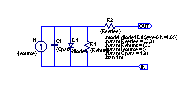
\includegraphics[width=\textwidth]{images/ltspice/singlecell.eps}
    \caption{%
        Schaltung        zur         Simulation        einer        Solarzelle
        gem\"ass        Abbildung       \ref{fig:circuit:solarCell}        von
        Seite     \pageref{fig:circuit:solarCell}. Die     Solarmodule     aus
        den     Abbildungen    \ref{fig:ltspice:module:cellBased:36x2}     und
        \ref{fig:ltspice:module:cellBased:72x1}  basieren auf  Zellen gem\"ass
        diesem Schaltschema.%
    }
    \label{fig:ltspice:solarCell}
\end{figure}

\begin{figure}[h!tb]
    \centering
    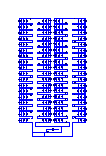
\includegraphics[width=\textwidth]{images/ltspice/module-72cells.eps}
    \caption{%
        Solarmodul     \"ahnlich     zu    Sunset     Solargenerator     AS150
        \cite{ref:solar:as150}, modelliert durch 2  parallele Str\"ange mit je
        36 Zellen gem\"ass Abbildung \ref{fig:ltspice:solarCell} in Serie.%
    }
    \label{fig:ltspice:module:cellBased:36x2}
\end{figure}

\begin{figure}[h!tb]
    \centering
    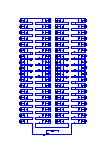
\includegraphics[width=\textwidth]{images/ltspice/module-72cells-series.eps}
    \caption{%
        Solarmodul   \"ahnlich   zu   Sunmodule  Pro-Series   XL   SW320   aus
        \cite{ref:solar:sunmodulePro},  modelliert durch  einen Strang  mit 72
        Zellen gem\"ass Abbildung \ref{fig:ltspice:solarCell} in Serie.%
    }
    \label{fig:ltspice:module:cellBased:72x1}
\end{figure}
\todo{Transistoren aus Schaltbildern entfernen, IN/OUT benennen, Abbildung sollte nur Modul sein}


% ---------------------------------------------------------------------------- %
\clearpage
\section{Vereinfachtes Modell f\"ur ein PV-Modul}
\label{app:models:develop:module:simple}
% ---------------------------------------------------------------------------- %

Zur  Reduktion des  Rechenaufwands im  Vergleich zu  dem im  vorigen Abschnitt
entwickelten Modell soll ein vereinfachtes Modell eines Solarmoduls entwickelt
werden.

Ausgangspunkt   ist   das   Eindiodenmodell    einer   Zelle   aus   Abbildung
\todo{reference}, f\"ur  welches die Parameter  so angepasst werden,  dass das
Verhalten des aus Zellen aufgebauten Modells aus dem vorigen Abschnitt und des
vereinfachten Modells zufriedenstellend \"ubereinstimmen.

Das Vorgehen ist dabei wie folgt: \todo{Eigentliche Werte}

\begin{itemize}
    \item
        Die parasit\"are  Kapazit\"at des  Moduls wird angepasst  gem\"ass dem
        Gesetz zur Serieschaltung von Kapazit\"aten:
        $C_{\mathrm{p, Modul}} = C_{\mathrm{p, Zelle}} \div \text{Anzahl Zellen}$
    \item
        Der Seriewiderstand des Moduls ist die Summe der Seriewiderst\"ande aller
        Zellen
    \item
        Der  Parallele   Widerstand  wird   entsprechend  der   Anzahl  Zellen
        hochgerechnet.
        \todo{kein Einfluss, verifikation}
    \item
        Der Reverse  Saturation Current  des Moduls ist  von der  Fl\"ache des
        Moduls abh\"angig und  wird als Startwert vorerst  gem\"ass der Anzahl
        Module hochgerechnet.
    \item
        Der  Idealit\"atsfaktor ist  ein Indikator  f\"ur den  Spannungsabfall
        \"uber   einer   Diode   bei   einem   bestimmten   Strom   \todo{ref:
        abbildung}. Bei  einer Serieschaltung  von Dioden  sollte entsprechend
        mehr   Spannung    \"uber   dem   gesamten   Strang    abfallen   (bei
        gleichbleibendem  Strom). Der Startwert  f\"ur den  Idealit\"atsfaktor
        des vereinfachten Modells wird  deshalb entsprechend der Anzahl Zellen
        im Modul skaliert.
\end{itemize}

Gem\"ass dieser Methodik werden die Startwerte festgelegt auf:

\begin{itemize}
    \firmlist
    \item
        $C_{\mathrm{p, Modul}} = \SI{167}{\nano\farad}$
    \item
        $R_{\mathrm{S}} = \SI{12}{\milli\ohm}$
    \item
        $R_{\mathrm{Shunt}} = \SI{60}{\kilo\ohm}$
    \item
        $I_{\mathrm{S}} = \SI{288}{\milli\ampere}$
    \item
        $n = 118$
\end{itemize}

Mit diesen  Werten werden verschiedene  Szenarien simuliert und  die Resultate
mit den  Ergebnissen des komplexeren Modells  verglichen. Durch Iteration wird
$I_{\mathrm{S}}$ schlussendlich  auf \SI{2.88}{\micro\ampere}  festgelegt, was
kurioserweise kleiner ist als der Wert einer einzelnen Diode.

Abbildungen
\ref{fig:model:simpel:verif:current:mosfet:freq},
\ref{fig:model:simpel:verif:voltage:mosfet:freq},
\ref{fig:model:simpel:verif:current:RL:freq} und
\ref{fig:model:simpel:verif:current:mosfet:time} stellen die Resultate
verschiedener Simulationen mit und ohne Last f\"ur das vereinfachte Modell und
das zellenbasierte  Modell graphisch dar.   Wie zu erkennen ist,  besteht eine
gute \"Ubereinstimmung.

%Parasit\"are Kapazit\"at: Kapazit\"at einer Zelle / anzahl Zellen \\
%Serie widerstand: widerstand einzelzelle * anzahl zellen \\
%shunt widerstand: widerstand einer zelle / anzahl zellen \\
%IS: IS einzelzelle * anzahl zellen (0.288m) -> anpassen, bis frequenzgang und zeitplot passend \\
%N: N einzelzelle * anzahl zellen \\
%Shockley diode model \\
\todo{Einheiten achsen, auflistung parameter, schaltkreise zu plots, LTspice diagramme}


\begin{figure}
    \begin{tikzpicture}
       \begin{scope}[x={(0mm,0mm)},y={(90mm,0.9\textwidth)}]
           \begin{axis}[%
                   xmode=log,
                   height=45mm,
                   width=0.9\textwidth,
                   at={(0,45mm)},
                   grid=both,
                   xlabel=Frequenz (\si{\hertz}),
                   ylabel=Strom (\si{\deci\bel}),
               ]
                \addplot[color=blue] table {data/simple-model-verification/module-72cells-series--reference--freq-sweep-over-mosfet-no-load--I--magn.dat};
                \addplot[color=magenta] table {data/simple-model-verification/module-simple-72x1--freq-sqeep-over-mosfet-no-load--I--magn.dat};
           \end{axis}
           \begin{axis}[%
                   xmode=log,
                   height=45mm,
                   width=0.9\textwidth,
                   at={(0,0)},
                   grid=both,
                   xlabel=Frequenz (\si{\hertz}),
                   ylabel=Phase (\si{\degree}),
               ]
                \addplot[color=blue] table {data/simple-model-verification/module-72cells-series--reference--freq-sweep-over-mosfet-no-load--I--phase.dat};
                \addplot[color=magenta] table {data/simple-model-verification/module-simple-72x1--freq-sqeep-over-mosfet-no-load--I--phase.dat};
           \end{axis}
       \end{scope}
   \end{tikzpicture}
    \caption{Frequenzgang des Stroms durch den MOSFET bei einer Beschaltung ohne zus\"atzliche Last}
    \label{fig:model:simpel:verif:current:mosfet:freq}
\end{figure}

\begin{figure}
    \begin{tikzpicture}
       \begin{scope}[x={(0mm,0mm)},y={(90mm,0.9\textwidth)}]
           \begin{axis}[%
                   xmode=log,
                   height=45mm,
                   width=0.9\textwidth,
                   at={(0,45mm)},
                   grid=both,
                   xlabel=Frequenz (\si{\hertz}),
                   ylabel=Spannung (\si{\deci\bel}),
               ]
                \addplot[color=blue] table {data/simple-model-verification/module-72cells-series--reference--freq-sweep-over-mosfet-no-load--U--magn.dat};
                \addplot[color=magenta] table {data/simple-model-verification/module-simple-72x1--freq-sweep-over-mosfet-no-load--U--magn.dat};
           \end{axis}
           \begin{axis}[%
                   xmode=log,
                   height=45mm,
                   width=0.9\textwidth,
                   at={(0,0)},
                   grid=both,
                   xlabel=Frequenz (\si{\hertz}),
                   ylabel=Phase (\si{\degree}),
               ]
                \addplot[color=blue] table {data/simple-model-verification/module-72cells-series--reference--freq-sweep-over-mosfet-no-load--U--phase.dat};
                \addplot[color=magenta] table {data/simple-model-verification/module-simple-72x1--freq-sweep-over-mosfet-no-load--U--phase.dat};
           \end{axis}
       \end{scope}
   \end{tikzpicture}
    \caption{Frequenzgang der Spannung \"uber dem MOSFET bei einer Beschaltung ohne zus\"atzliche Last}
    \label{fig:model:simpel:verif:voltage:mosfet:freq}
\end{figure}

\begin{figure}
    \begin{tikzpicture}
       \begin{scope}[x={(0mm,0mm)},y={(90mm,0.9\textwidth)}]
           \begin{axis}[%
                   xmode=log,
                   height=45mm,
                   width=0.9\textwidth,
                   at={(0,45mm)},
                   grid=both,
                   xlabel=Frequenz (\si{\hertz}),
                   ylabel=Spannung (\si{\deci\bel}),
               ]
                \addplot[color=blue] table {data/simple-model-verification/module-72cells-series--reference--freq-sweep-over-Rload--100ohm-100uF--I--magn.dat};
                \addplot[color=magenta] table {data/simple-model-verification/module-simple-72x1--freq-sweep-over-Rload--100ohm-100uF--I--magn.dat};
           \end{axis}
           \begin{axis}[%
                   xmode=log,
                   height=45mm,
                   width=0.9\textwidth,
                   at={(0,0)},
                   grid=both,
                   xlabel=Frequenz (\si{\hertz}),
                   ylabel=Phase (\si{\degree}),
               ]
                \addplot[color=blue] table {data/simple-model-verification/module-72cells-series--reference--freq-sweep-over-Rload--100ohm-100uF--I--phase.dat};
                \addplot[color=magenta] table {data/simple-model-verification/module-simple-72x1--freq-sweep-over-Rload--100ohm-100uF--I--phase.dat};
           \end{axis}
       \end{scope}
   \end{tikzpicture}
   \caption{Frequenzgang des Stroms durch den Lastwiderstand bei einer Last von \SI{100}{\ohm} parallel zu \SI{100}{\micro\farad}}
    \label{fig:model:simpel:verif:current:RL:freq}
   %\label{fig:freqresponse:module:simple}
\end{figure}


\begin{figure}
    \begin{tikzpicture}
       \begin{scope}[x={(0mm,0mm)},y={(60mm,0.9\textwidth)}]
           \begin{axis}[%
                   height=60mm,
                   width=0.9\textwidth,
                   at={(0,0)},
                   grid=both,
                   xlabel=Zeit (\si{\second}),
                   ylabel=Strom (\si{\ampere}),
               ]
                \addplot[color=blue] table {data/simple-model-verification/module-72cells-series--reference--time-domain-over-mosfet-10kHz--I.dat};
                \addplot[color=magenta] table {data/simple-model-verification/module-simple-72x1--time-domain-over-mosfet--10kHz--I.dat};
           \end{axis}
       \end{scope}
   \end{tikzpicture}
    \caption{Zeitlicher Verlauf des Stroms durch den MOSFET bei einer Beschaltung ohne zus\"atzliche Last}
    \label{fig:model:simpel:verif:current:mosfet:time}
\end{figure}


% ---------------------------------------------------------------------------- %
\clearpage
\section{DC-Leitung}
\label{app:models:develop:DCLine}
% ---------------------------------------------------------------------------- %

\todo{Induktivit\"at}
\todo{Kapazit\"at}

%% **************************************************************************** %
\chapter{Zusatzinformationen zur Modellentwicklung}
\label{app:models:calcs}
% **************************************************************************** %

Dieses Kapitel beinhaltet Berechnungen, welche zur Modellierung benutzt werden
und aus Gr\"unden der \"Ubersichtlichkeit nicht im Hauptteil zu finden sind.


% ---------------------------------------------------------------------------- %
\section{Referenzwerte f\"ur PV-Zelle}
\label{app:models:develop:cell}
% ---------------------------------------------------------------------------- %

Zur  Herleitung  der  Zellenparameter  werden vier  Quellen  herangezogen,  um
ein  einigermassen  gut  abgest\"utztes Ergebnis  zu  erhalten. Die  gesuchten
Parameter sollen  f\"ur am Markt  erh\"altliche Module g\"ultig  sein, weshalb
Datenbl\"atter von Solar\emph{modulen} und nicht Zellen verwendet werden.

Zuerst  werden  Zellenstrom  und Zellenspannung  bestimmt,  anschliessend  die
Fl\"ache einer Zelle,  um damit auf die im Modell  verwendete Kapazit\"at, den
Shunt-Widerstand und den Seriewiderstand schliessen zu k\"onnen.


\begin{table}
    \centering
    \small
    \caption{%
        Daten   f\"ur   Solarmodule.  \textbf{pk}:   polykristallines   Panel,
        \textbf{mk}:     monokristallines     Panel.     \emph{Anmerkung}: Die
        Konfiguration  der Module  (wieviele  Zellen in  Serie  und wie  viele
        Str\"ange  parallel)  ist  mit   Ausnahme  des  Solarex  MSX-60  nicht
        angegeben. Es  ist  aber  bekannt,  in  welcher  Gr\"ossenordnung  die
        Spannung  pro  Zelle  ungef\"ahr  liegen sollte,  womit  man  aus  den
        angegebenen  Leerlaufspannungen  und  der Gesamtzahl  Zellen  auf  die
        Konfiguration eines Modules schliessen kann.%
    }
    \label{tab:moduleData:IU}
    \begin{tabular}{lp{20mm}lllll}
        \toprule
          \rotatebox{70}{\pbox{25mm}{Quelle}}
        & \rotatebox{70}{\pbox{25mm}{Modell}}
        & \rotatebox{70}{\pbox{25mm}{Kurzschluss-\\strom $I_{\mathrm{SC}}$}}
        & \rotatebox{70}{\pbox{25mm}{Leerlauf-\\spannung $V_{\mathrm{OC}}$}}
        & \rotatebox{70}{\pbox{25mm}{Anzahl Zellen \\(total)}}
        & \rotatebox{70}{\pbox{25mm}{Anzahl Zellen \\(Strang)}}
        & \rotatebox{70}{\pbox{25mm}{Leerlaufspan-\\nung pro Zelle}} \\
        \midrule

          \cite{ref:solar:bonkoungou}
        & Solarex MSX-60
        & \SI{3.8}{\ampere}
        & \SI{21.1}{\volt}
        & \num{36}
        & \num{36}
        & \SI{586}{\milli\volt}
        \\

          \cite{ref:solar:px85}
        & Sunset PX85 (\textbf{pk})
        & \SI{5.5}{\ampere}
        & \SI{21.5}{\volt}
        & \num{76}
        & \num{38}
        & \SI{566}{\milli\volt}
        \\

          \cite{ref:solar:as150}
        & Sunset Solargenerator AS150 (\textbf{mk})
        & \SI{8.7}{\ampere}
        & \SI{22.3}{\volt}
        & \num{36}
        & \num{36}
        & \SI{620}{\milli\volt}
        \\

          \cite{ref:solar:sunmodulePro}
        & Sunmodule Pro-Series XL SW320 (\textbf{mk})
        & \SI{9.41}{\ampere}
        & \SI{45.9}{\volt}
        & \num{72}
        & \num{72}
        & \SI{638}{\milli\volt}
        \\

        \bottomrule
    \end{tabular}
\end{table}

\myfancybreak

Tabelle  \ref{tab:moduleData:IU} enth\"alt  die Daten  zu Kurzschlussstr\"omen
und Leerlaufspannungen von vier Modulen. Die Spannung $U_{\mathrm{OC, Zelle}}$
pro Zelle (letzte Spalte) errechnet sich gem\"ass:

\begin{equation}
    \label{eq:voltagePerCell}
    U_{\mathrm{OC, Zelle}} = \frac{U_{\mathrm{OC, Strang}}}{\text{Anzahl Zellen pro Strang}}
\end{equation}

Wir verwenden f\"ur  die Simulation einer Zelle den  gerundeten Mittelwert der
Zellenspannungen aus der letzten Spalte von Tabelle \ref{tab:moduleData:IU}:

\begin{equation}
    \label{eq:cell:UOC}
    \underline{\underline{U_{\mathrm{OC, Zelle, Simu}} = \SI{600}{\milli\volt}}}
\end{equation}

Polykristalline  Zellen  liefern  bedeutend  kleinere  Kurzschlusstr\"ome  als
monokristalline  Zellen.  Jedoch  werden bei  monokristallinen Zellen  weniger
Str\"ange parallel  geschaltet, womit  der Gesamtstrom  des Moduls  immer noch
unter \SI{10}{\ampere}  bleibt. Unabh\"angig vom  genauen Aufbau  eines Moduls
gehen wir  daher davon aus,  dass es  nicht mehr als  \SI{10}{\ampere} liefern
wird.

\myfancybreak

Das    PX-85-Modul   aus    \cite{ref:solar:px85}    verwendet   76    Zellen,
angeordnet  in   einer  $4  \times  19$   -  Konfiguration. Seine  Abmessungen
betragen   $\SI{1477}{\milli\meter}    \times   \SI{660}{\milli\meter}$,   was
sich   herunterrechnen  l\"asst   auf  eine   ungef\"ahre  Modulgr\"osse   von
$\SI{165}{\milli\meter}   \times   \SI{75}{\milli\meter}$. Dabei  werden   die
Abmessungen   des   Rahmens   und   die  Abst\"ande   zwischen   den   Modulen
vernachl\"assigt.

Die Fl\"ache  des AS-150-Moduls wird analog  aus Quelle~\cite{ref:solar:as150}
zu  $\SI{155}{\milli\meter}  \times   \SI{164}{\milli\meter}$  bestimmt.   Das
XL-320-Modul   aus   \cite{ref:solar:sunmodulePro}    hat   die   Zellgr\"osse
direkt    angegeben,    sie     betr\"agt    $\SI{156}{\milli\meter}    \times
\SI{156}{\milli\meter}$. Es ist naheliegend dass aufgrund von Standardisierung
das AS-150-Modul die gleiche Zelldimension hat wie das XL-320-Modul, n\"amlich
den verbreiteten 6-Zoll-Formfaktor.

Da  eine gr\"ossere  Zelle eine  gr\"ossere Kapazit\"at  und somit  gr\"ossere
Probleme   im  Falle   der  Kurzschlussvariante   bedeutet,  wird   mit  einer
Zellgr\"osse   von   $\SI{156}{\milli\meter}  \times   \SI{156}{\milli\meter}$
gerechnet, womit sich die Fl\"ache der Zelle bestimmt zu:

\begin{equation}
    \label{eq:cell:surface}
    \underline{\underline{A_{\mathrm{Zelle}} = \SI{156}{\milli\meter} \times \SI{156}{\milli\meter} = \SI{243.36}{\centi\meter\squared}}}
\end{equation}

Dies     entspricht     ungef\"ahr     der     600-fachen     Fl\"ache     des
\SI{0.43}{\centi\meter\squared}-Modules aus  Quelle \cite{ref:solar:scofield}.


% ---------------------------------------------------------------------------- %
\section{Zusatzinformationen zu Dioden}
\label{app:sec:cell:diodeInfo}
% ---------------------------------------------------------------------------- %

Dieser  Abschnitt beinhaltet  einige  allgemeine Hintergrundinformationen  zur
Modellierung  von Dioden,  welche benutzt  werden, um  den Reverse  Saturation
Current $I_{\mathrm{S}}$  und den  Idealit\"atsfaktor $n$ zu  bestimmen (siehe
Abschnitt \ref{sec:simu:model:cell}, Seite \pageref{sec:simu:model:cell}).

Die  Grundlage   f\"ur  das  Diodenmodell  ist   die  Shockley-Diodengleichung
\cite{ref:solar:shockleyEquation}.

\begin{equation}
    \label{eq:diode}
    I_{\mathrm{D}} = I_{\mathrm{S}} \cdot \left( \exp\left(\frac{q \cdot V}{n \cdot k \cdot T}\right) - 1 \right)
\end{equation}

\begin{conditions}
    I_{\mathrm{D}} & Diodenstrom \\
    I_{\mathrm{S}} & Reverse saturation current \\
    q              & Elementarladung eines Elektrons (\SI{1.602e-19}{\coulomb}) \\
    V              & Diodenspannung \\
    n              & Idealit\"atsfaktor \\
    k              & Boltzmannkonstante (\SI{1.38e-23}{\joule\per\kelvin}) \\
    T              & Diodentemperatur \\
\end{conditions}

Der   Reverse   Saturation  Current   ist   der   Strom,  der   beim   Anlegen
einer  negativen   Spannung  \"uber  die   Diode  fliesst,  bevor   die  Diode
durchbricht~\cite{ref:solar:diodeCharacteristics}.    Er  liegt   bei  kleinen
Dioden \"ublicherweise Bereich von Nano-Amp\`ere bis Femto-Amp\`ere\todo{F\"ur
k\"aufliche Dioden, nicht  Solarzellen}, bei einer Solarzelle  ist er h\"oher,
da diese gr\"osser ist.

Wie  man an  Gleichung \ref{eq:diode}  erkennen kann,  steigt der  Diodenstrom
f\"ur eine gegebene Spannung, wenn der Reverse Saturation Current ansteigt.

Der Idealit\"atsfaktor ist ein Indikator  f\"ur den Spannungsabfall \"uber der
Diode in  Abh\"angigkeit des durchfliessenden Stromes  und liegt normalerweise
zwischen 1  (ideale Diode)  und 2. Unter besonderen  Umst\"anden kann  er auch
h\"oher  sein, z.B.  bei  der Modellierung  von mehreren  zusammengeschalteten
Dioden   (siehe    Abschnitt   \ref{app:models:develop:module:simple},   Seite
\pageref{app:models:develop:module:simple}).

Je  gr\"osser   der  Idealit\"atsfaktor,  umso  h\"oher   der  Spannungsabfall
\"uber  der  Diode  f\"ur  einen   gegebenen  Strom  (bzw.  umso  kleiner  der
Strom  bei  einer  fixen   Spannung). Der  Einfluss  von  $_{\mathrm{S}}$  und
$n$  auf  die  Strom-Spannungs-Kennlinie   einer  Diode  sind  vereinfacht  in
Abbildung \ref{fig:diodeVI:IS}  dargestellt. Grundlage der Kurve ist  die oben
aufgef\"uhrte Shockley-Diodengleichung.

\begin{figure}[h!tb]
    \centering
    %% Creator: Matplotlib, PGF backend
%%
%% To include the figure in your LaTeX document, write
%%   \input{<filename>.pgf}
%%
%% Make sure the required packages are loaded in your preamble
%%   \usepackage{pgf}
%%
%% Figures using additional raster images can only be included by \input if
%% they are in the same directory as the main LaTeX file. For loading figures
%% from other directories you can use the `import` package
%%   \usepackage{import}
%% and then include the figures with
%%   \import{<path to file>}{<filename>.pgf}
%%
%% Matplotlib used the following preamble
%%   \usepackage{fontspec}
%%   \setmainfont{Bitstream Vera Serif}
%%   \setsansfont{Bitstream Vera Sans}
%%   \setmonofont{Bitstream Vera Sans Mono}
%%
\begingroup%
\makeatletter%
\begin{pgfpicture}%
\pgfpathrectangle{\pgfpointorigin}{\pgfqpoint{4.500000in}{4.000000in}}%
\pgfusepath{use as bounding box, clip}%
\begin{pgfscope}%
\pgfsetbuttcap%
\pgfsetmiterjoin%
\pgfsetlinewidth{0.000000pt}%
\definecolor{currentstroke}{rgb}{0.000000,0.000000,0.000000}%
\pgfsetstrokecolor{currentstroke}%
\pgfsetstrokeopacity{0.000000}%
\pgfsetdash{}{0pt}%
\pgfpathmoveto{\pgfqpoint{0.000000in}{0.000000in}}%
\pgfpathlineto{\pgfqpoint{4.500000in}{0.000000in}}%
\pgfpathlineto{\pgfqpoint{4.500000in}{4.000000in}}%
\pgfpathlineto{\pgfqpoint{0.000000in}{4.000000in}}%
\pgfpathclose%
\pgfusepath{}%
\end{pgfscope}%
\begin{pgfscope}%
\pgfsetbuttcap%
\pgfsetmiterjoin%
\pgfsetlinewidth{0.000000pt}%
\definecolor{currentstroke}{rgb}{0.000000,0.000000,0.000000}%
\pgfsetstrokecolor{currentstroke}%
\pgfsetstrokeopacity{0.000000}%
\pgfsetdash{}{0pt}%
\pgfpathmoveto{\pgfqpoint{0.450000in}{0.400000in}}%
\pgfpathlineto{\pgfqpoint{4.050000in}{0.400000in}}%
\pgfpathlineto{\pgfqpoint{4.050000in}{3.600000in}}%
\pgfpathlineto{\pgfqpoint{0.450000in}{3.600000in}}%
\pgfpathclose%
\pgfusepath{}%
\end{pgfscope}%
\begin{pgfscope}%
\pgfpathrectangle{\pgfqpoint{0.450000in}{0.400000in}}{\pgfqpoint{3.600000in}{3.200000in}} %
\pgfusepath{clip}%
\pgfsetbuttcap%
\pgfsetroundjoin%
\definecolor{currentfill}{rgb}{1.000000,0.000000,1.000000}%
\pgfsetfillcolor{currentfill}%
\pgfsetfillopacity{0.500000}%
\pgfsetlinewidth{0.000000pt}%
\definecolor{currentstroke}{rgb}{1.000000,0.000000,1.000000}%
\pgfsetstrokecolor{currentstroke}%
\pgfsetstrokeopacity{0.500000}%
\pgfsetdash{}{0pt}%
\pgfpathmoveto{\pgfqpoint{1.850000in}{2.000000in}}%
\pgfpathlineto{\pgfqpoint{1.850000in}{1.599790in}}%
\pgfpathlineto{\pgfqpoint{1.850822in}{1.599812in}}%
\pgfpathlineto{\pgfqpoint{1.851643in}{1.599835in}}%
\pgfpathlineto{\pgfqpoint{1.852465in}{1.599857in}}%
\pgfpathlineto{\pgfqpoint{1.853287in}{1.599880in}}%
\pgfpathlineto{\pgfqpoint{1.854108in}{1.599904in}}%
\pgfpathlineto{\pgfqpoint{1.854930in}{1.599927in}}%
\pgfpathlineto{\pgfqpoint{1.855752in}{1.599951in}}%
\pgfpathlineto{\pgfqpoint{1.856573in}{1.599975in}}%
\pgfpathlineto{\pgfqpoint{1.857395in}{1.600000in}}%
\pgfpathlineto{\pgfqpoint{1.858216in}{1.600024in}}%
\pgfpathlineto{\pgfqpoint{1.859038in}{1.600049in}}%
\pgfpathlineto{\pgfqpoint{1.859860in}{1.600075in}}%
\pgfpathlineto{\pgfqpoint{1.860681in}{1.600100in}}%
\pgfpathlineto{\pgfqpoint{1.861503in}{1.600126in}}%
\pgfpathlineto{\pgfqpoint{1.862325in}{1.600153in}}%
\pgfpathlineto{\pgfqpoint{1.863146in}{1.600179in}}%
\pgfpathlineto{\pgfqpoint{1.863968in}{1.600206in}}%
\pgfpathlineto{\pgfqpoint{1.864790in}{1.600233in}}%
\pgfpathlineto{\pgfqpoint{1.865611in}{1.600261in}}%
\pgfpathlineto{\pgfqpoint{1.866433in}{1.600289in}}%
\pgfpathlineto{\pgfqpoint{1.867255in}{1.600317in}}%
\pgfpathlineto{\pgfqpoint{1.868076in}{1.600346in}}%
\pgfpathlineto{\pgfqpoint{1.868898in}{1.600375in}}%
\pgfpathlineto{\pgfqpoint{1.869719in}{1.600404in}}%
\pgfpathlineto{\pgfqpoint{1.870541in}{1.600434in}}%
\pgfpathlineto{\pgfqpoint{1.871363in}{1.600464in}}%
\pgfpathlineto{\pgfqpoint{1.872184in}{1.600495in}}%
\pgfpathlineto{\pgfqpoint{1.873006in}{1.600525in}}%
\pgfpathlineto{\pgfqpoint{1.873828in}{1.600557in}}%
\pgfpathlineto{\pgfqpoint{1.874649in}{1.600588in}}%
\pgfpathlineto{\pgfqpoint{1.875471in}{1.600620in}}%
\pgfpathlineto{\pgfqpoint{1.876293in}{1.600653in}}%
\pgfpathlineto{\pgfqpoint{1.877114in}{1.600685in}}%
\pgfpathlineto{\pgfqpoint{1.877936in}{1.600718in}}%
\pgfpathlineto{\pgfqpoint{1.878758in}{1.600752in}}%
\pgfpathlineto{\pgfqpoint{1.879579in}{1.600786in}}%
\pgfpathlineto{\pgfqpoint{1.880401in}{1.600820in}}%
\pgfpathlineto{\pgfqpoint{1.881222in}{1.600855in}}%
\pgfpathlineto{\pgfqpoint{1.882044in}{1.600891in}}%
\pgfpathlineto{\pgfqpoint{1.882866in}{1.600926in}}%
\pgfpathlineto{\pgfqpoint{1.883687in}{1.600962in}}%
\pgfpathlineto{\pgfqpoint{1.884509in}{1.600999in}}%
\pgfpathlineto{\pgfqpoint{1.885331in}{1.601036in}}%
\pgfpathlineto{\pgfqpoint{1.886152in}{1.601074in}}%
\pgfpathlineto{\pgfqpoint{1.886974in}{1.601111in}}%
\pgfpathlineto{\pgfqpoint{1.887796in}{1.601150in}}%
\pgfpathlineto{\pgfqpoint{1.888617in}{1.601189in}}%
\pgfpathlineto{\pgfqpoint{1.889439in}{1.601228in}}%
\pgfpathlineto{\pgfqpoint{1.890261in}{1.601268in}}%
\pgfpathlineto{\pgfqpoint{1.891082in}{1.601308in}}%
\pgfpathlineto{\pgfqpoint{1.891904in}{1.601349in}}%
\pgfpathlineto{\pgfqpoint{1.892725in}{1.601391in}}%
\pgfpathlineto{\pgfqpoint{1.893547in}{1.601432in}}%
\pgfpathlineto{\pgfqpoint{1.894369in}{1.601475in}}%
\pgfpathlineto{\pgfqpoint{1.895190in}{1.601518in}}%
\pgfpathlineto{\pgfqpoint{1.896012in}{1.601561in}}%
\pgfpathlineto{\pgfqpoint{1.896834in}{1.601605in}}%
\pgfpathlineto{\pgfqpoint{1.897655in}{1.601649in}}%
\pgfpathlineto{\pgfqpoint{1.898477in}{1.601694in}}%
\pgfpathlineto{\pgfqpoint{1.899299in}{1.601740in}}%
\pgfpathlineto{\pgfqpoint{1.900120in}{1.601786in}}%
\pgfpathlineto{\pgfqpoint{1.900942in}{1.601833in}}%
\pgfpathlineto{\pgfqpoint{1.901764in}{1.601880in}}%
\pgfpathlineto{\pgfqpoint{1.902585in}{1.601928in}}%
\pgfpathlineto{\pgfqpoint{1.903407in}{1.601976in}}%
\pgfpathlineto{\pgfqpoint{1.904228in}{1.602025in}}%
\pgfpathlineto{\pgfqpoint{1.905050in}{1.602075in}}%
\pgfpathlineto{\pgfqpoint{1.905872in}{1.602125in}}%
\pgfpathlineto{\pgfqpoint{1.906693in}{1.602176in}}%
\pgfpathlineto{\pgfqpoint{1.907515in}{1.602228in}}%
\pgfpathlineto{\pgfqpoint{1.908337in}{1.602280in}}%
\pgfpathlineto{\pgfqpoint{1.909158in}{1.602333in}}%
\pgfpathlineto{\pgfqpoint{1.909980in}{1.602386in}}%
\pgfpathlineto{\pgfqpoint{1.910802in}{1.602440in}}%
\pgfpathlineto{\pgfqpoint{1.911623in}{1.602495in}}%
\pgfpathlineto{\pgfqpoint{1.912445in}{1.602550in}}%
\pgfpathlineto{\pgfqpoint{1.913267in}{1.602606in}}%
\pgfpathlineto{\pgfqpoint{1.914088in}{1.602663in}}%
\pgfpathlineto{\pgfqpoint{1.914910in}{1.602720in}}%
\pgfpathlineto{\pgfqpoint{1.915731in}{1.602779in}}%
\pgfpathlineto{\pgfqpoint{1.916553in}{1.602837in}}%
\pgfpathlineto{\pgfqpoint{1.917375in}{1.602897in}}%
\pgfpathlineto{\pgfqpoint{1.918196in}{1.602957in}}%
\pgfpathlineto{\pgfqpoint{1.919018in}{1.603018in}}%
\pgfpathlineto{\pgfqpoint{1.919840in}{1.603080in}}%
\pgfpathlineto{\pgfqpoint{1.920661in}{1.603143in}}%
\pgfpathlineto{\pgfqpoint{1.921483in}{1.603206in}}%
\pgfpathlineto{\pgfqpoint{1.922305in}{1.603270in}}%
\pgfpathlineto{\pgfqpoint{1.923126in}{1.603335in}}%
\pgfpathlineto{\pgfqpoint{1.923948in}{1.603401in}}%
\pgfpathlineto{\pgfqpoint{1.924770in}{1.603467in}}%
\pgfpathlineto{\pgfqpoint{1.925591in}{1.603534in}}%
\pgfpathlineto{\pgfqpoint{1.926413in}{1.603603in}}%
\pgfpathlineto{\pgfqpoint{1.927234in}{1.603671in}}%
\pgfpathlineto{\pgfqpoint{1.928056in}{1.603741in}}%
\pgfpathlineto{\pgfqpoint{1.928878in}{1.603812in}}%
\pgfpathlineto{\pgfqpoint{1.929699in}{1.603883in}}%
\pgfpathlineto{\pgfqpoint{1.930521in}{1.603956in}}%
\pgfpathlineto{\pgfqpoint{1.931343in}{1.604029in}}%
\pgfpathlineto{\pgfqpoint{1.932164in}{1.604103in}}%
\pgfpathlineto{\pgfqpoint{1.932986in}{1.604178in}}%
\pgfpathlineto{\pgfqpoint{1.933808in}{1.604254in}}%
\pgfpathlineto{\pgfqpoint{1.934629in}{1.604331in}}%
\pgfpathlineto{\pgfqpoint{1.935451in}{1.604409in}}%
\pgfpathlineto{\pgfqpoint{1.936273in}{1.604488in}}%
\pgfpathlineto{\pgfqpoint{1.937094in}{1.604567in}}%
\pgfpathlineto{\pgfqpoint{1.937916in}{1.604648in}}%
\pgfpathlineto{\pgfqpoint{1.938737in}{1.604730in}}%
\pgfpathlineto{\pgfqpoint{1.939559in}{1.604812in}}%
\pgfpathlineto{\pgfqpoint{1.940381in}{1.604896in}}%
\pgfpathlineto{\pgfqpoint{1.941202in}{1.604981in}}%
\pgfpathlineto{\pgfqpoint{1.942024in}{1.605066in}}%
\pgfpathlineto{\pgfqpoint{1.942846in}{1.605153in}}%
\pgfpathlineto{\pgfqpoint{1.943667in}{1.605241in}}%
\pgfpathlineto{\pgfqpoint{1.944489in}{1.605330in}}%
\pgfpathlineto{\pgfqpoint{1.945311in}{1.605420in}}%
\pgfpathlineto{\pgfqpoint{1.946132in}{1.605511in}}%
\pgfpathlineto{\pgfqpoint{1.946954in}{1.605603in}}%
\pgfpathlineto{\pgfqpoint{1.947776in}{1.605696in}}%
\pgfpathlineto{\pgfqpoint{1.948597in}{1.605791in}}%
\pgfpathlineto{\pgfqpoint{1.949419in}{1.605886in}}%
\pgfpathlineto{\pgfqpoint{1.950240in}{1.605983in}}%
\pgfpathlineto{\pgfqpoint{1.951062in}{1.606081in}}%
\pgfpathlineto{\pgfqpoint{1.951884in}{1.606180in}}%
\pgfpathlineto{\pgfqpoint{1.952705in}{1.606280in}}%
\pgfpathlineto{\pgfqpoint{1.953527in}{1.606382in}}%
\pgfpathlineto{\pgfqpoint{1.954349in}{1.606484in}}%
\pgfpathlineto{\pgfqpoint{1.955170in}{1.606588in}}%
\pgfpathlineto{\pgfqpoint{1.955992in}{1.606694in}}%
\pgfpathlineto{\pgfqpoint{1.956814in}{1.606800in}}%
\pgfpathlineto{\pgfqpoint{1.957635in}{1.606908in}}%
\pgfpathlineto{\pgfqpoint{1.958457in}{1.607017in}}%
\pgfpathlineto{\pgfqpoint{1.959279in}{1.607127in}}%
\pgfpathlineto{\pgfqpoint{1.960100in}{1.607239in}}%
\pgfpathlineto{\pgfqpoint{1.960922in}{1.607352in}}%
\pgfpathlineto{\pgfqpoint{1.961743in}{1.607467in}}%
\pgfpathlineto{\pgfqpoint{1.962565in}{1.607583in}}%
\pgfpathlineto{\pgfqpoint{1.963387in}{1.607700in}}%
\pgfpathlineto{\pgfqpoint{1.964208in}{1.607818in}}%
\pgfpathlineto{\pgfqpoint{1.965030in}{1.607939in}}%
\pgfpathlineto{\pgfqpoint{1.965852in}{1.608060in}}%
\pgfpathlineto{\pgfqpoint{1.966673in}{1.608183in}}%
\pgfpathlineto{\pgfqpoint{1.967495in}{1.608308in}}%
\pgfpathlineto{\pgfqpoint{1.968317in}{1.608434in}}%
\pgfpathlineto{\pgfqpoint{1.969138in}{1.608561in}}%
\pgfpathlineto{\pgfqpoint{1.969960in}{1.608690in}}%
\pgfpathlineto{\pgfqpoint{1.970782in}{1.608821in}}%
\pgfpathlineto{\pgfqpoint{1.971603in}{1.608953in}}%
\pgfpathlineto{\pgfqpoint{1.972425in}{1.609087in}}%
\pgfpathlineto{\pgfqpoint{1.973246in}{1.609222in}}%
\pgfpathlineto{\pgfqpoint{1.974068in}{1.609359in}}%
\pgfpathlineto{\pgfqpoint{1.974890in}{1.609498in}}%
\pgfpathlineto{\pgfqpoint{1.975711in}{1.609638in}}%
\pgfpathlineto{\pgfqpoint{1.976533in}{1.609780in}}%
\pgfpathlineto{\pgfqpoint{1.977355in}{1.609923in}}%
\pgfpathlineto{\pgfqpoint{1.978176in}{1.610069in}}%
\pgfpathlineto{\pgfqpoint{1.978998in}{1.610216in}}%
\pgfpathlineto{\pgfqpoint{1.979820in}{1.610365in}}%
\pgfpathlineto{\pgfqpoint{1.980641in}{1.610516in}}%
\pgfpathlineto{\pgfqpoint{1.981463in}{1.610668in}}%
\pgfpathlineto{\pgfqpoint{1.982285in}{1.610822in}}%
\pgfpathlineto{\pgfqpoint{1.983106in}{1.610979in}}%
\pgfpathlineto{\pgfqpoint{1.983928in}{1.611137in}}%
\pgfpathlineto{\pgfqpoint{1.984749in}{1.611296in}}%
\pgfpathlineto{\pgfqpoint{1.985571in}{1.611458in}}%
\pgfpathlineto{\pgfqpoint{1.986393in}{1.611622in}}%
\pgfpathlineto{\pgfqpoint{1.987214in}{1.611788in}}%
\pgfpathlineto{\pgfqpoint{1.988036in}{1.611955in}}%
\pgfpathlineto{\pgfqpoint{1.988858in}{1.612125in}}%
\pgfpathlineto{\pgfqpoint{1.989679in}{1.612297in}}%
\pgfpathlineto{\pgfqpoint{1.990501in}{1.612471in}}%
\pgfpathlineto{\pgfqpoint{1.991323in}{1.612646in}}%
\pgfpathlineto{\pgfqpoint{1.992144in}{1.612824in}}%
\pgfpathlineto{\pgfqpoint{1.992966in}{1.613004in}}%
\pgfpathlineto{\pgfqpoint{1.993788in}{1.613186in}}%
\pgfpathlineto{\pgfqpoint{1.994609in}{1.613371in}}%
\pgfpathlineto{\pgfqpoint{1.995431in}{1.613557in}}%
\pgfpathlineto{\pgfqpoint{1.996253in}{1.613746in}}%
\pgfpathlineto{\pgfqpoint{1.997074in}{1.613937in}}%
\pgfpathlineto{\pgfqpoint{1.997896in}{1.614130in}}%
\pgfpathlineto{\pgfqpoint{1.998717in}{1.614326in}}%
\pgfpathlineto{\pgfqpoint{1.999539in}{1.614524in}}%
\pgfpathlineto{\pgfqpoint{2.000361in}{1.614724in}}%
\pgfpathlineto{\pgfqpoint{2.001182in}{1.614926in}}%
\pgfpathlineto{\pgfqpoint{2.002004in}{1.615131in}}%
\pgfpathlineto{\pgfqpoint{2.002826in}{1.615339in}}%
\pgfpathlineto{\pgfqpoint{2.003647in}{1.615548in}}%
\pgfpathlineto{\pgfqpoint{2.004469in}{1.615761in}}%
\pgfpathlineto{\pgfqpoint{2.005291in}{1.615975in}}%
\pgfpathlineto{\pgfqpoint{2.006112in}{1.616193in}}%
\pgfpathlineto{\pgfqpoint{2.006934in}{1.616413in}}%
\pgfpathlineto{\pgfqpoint{2.007756in}{1.616635in}}%
\pgfpathlineto{\pgfqpoint{2.008577in}{1.616860in}}%
\pgfpathlineto{\pgfqpoint{2.009399in}{1.617088in}}%
\pgfpathlineto{\pgfqpoint{2.010220in}{1.617318in}}%
\pgfpathlineto{\pgfqpoint{2.011042in}{1.617551in}}%
\pgfpathlineto{\pgfqpoint{2.011864in}{1.617787in}}%
\pgfpathlineto{\pgfqpoint{2.012685in}{1.618026in}}%
\pgfpathlineto{\pgfqpoint{2.013507in}{1.618267in}}%
\pgfpathlineto{\pgfqpoint{2.014329in}{1.618511in}}%
\pgfpathlineto{\pgfqpoint{2.015150in}{1.618758in}}%
\pgfpathlineto{\pgfqpoint{2.015972in}{1.619008in}}%
\pgfpathlineto{\pgfqpoint{2.016794in}{1.619261in}}%
\pgfpathlineto{\pgfqpoint{2.017615in}{1.619517in}}%
\pgfpathlineto{\pgfqpoint{2.018437in}{1.619776in}}%
\pgfpathlineto{\pgfqpoint{2.019259in}{1.620038in}}%
\pgfpathlineto{\pgfqpoint{2.020080in}{1.620303in}}%
\pgfpathlineto{\pgfqpoint{2.020902in}{1.620571in}}%
\pgfpathlineto{\pgfqpoint{2.021723in}{1.620842in}}%
\pgfpathlineto{\pgfqpoint{2.022545in}{1.621116in}}%
\pgfpathlineto{\pgfqpoint{2.023367in}{1.621393in}}%
\pgfpathlineto{\pgfqpoint{2.024188in}{1.621674in}}%
\pgfpathlineto{\pgfqpoint{2.025010in}{1.621958in}}%
\pgfpathlineto{\pgfqpoint{2.025832in}{1.622245in}}%
\pgfpathlineto{\pgfqpoint{2.026653in}{1.622535in}}%
\pgfpathlineto{\pgfqpoint{2.027475in}{1.622829in}}%
\pgfpathlineto{\pgfqpoint{2.028297in}{1.623126in}}%
\pgfpathlineto{\pgfqpoint{2.029118in}{1.623427in}}%
\pgfpathlineto{\pgfqpoint{2.029940in}{1.623731in}}%
\pgfpathlineto{\pgfqpoint{2.030762in}{1.624039in}}%
\pgfpathlineto{\pgfqpoint{2.031583in}{1.624350in}}%
\pgfpathlineto{\pgfqpoint{2.032405in}{1.624665in}}%
\pgfpathlineto{\pgfqpoint{2.033226in}{1.624983in}}%
\pgfpathlineto{\pgfqpoint{2.034048in}{1.625305in}}%
\pgfpathlineto{\pgfqpoint{2.034870in}{1.625631in}}%
\pgfpathlineto{\pgfqpoint{2.035691in}{1.625960in}}%
\pgfpathlineto{\pgfqpoint{2.036513in}{1.626293in}}%
\pgfpathlineto{\pgfqpoint{2.037335in}{1.626630in}}%
\pgfpathlineto{\pgfqpoint{2.038156in}{1.626971in}}%
\pgfpathlineto{\pgfqpoint{2.038978in}{1.627316in}}%
\pgfpathlineto{\pgfqpoint{2.039800in}{1.627664in}}%
\pgfpathlineto{\pgfqpoint{2.040621in}{1.628017in}}%
\pgfpathlineto{\pgfqpoint{2.041443in}{1.628374in}}%
\pgfpathlineto{\pgfqpoint{2.042265in}{1.628734in}}%
\pgfpathlineto{\pgfqpoint{2.043086in}{1.629099in}}%
\pgfpathlineto{\pgfqpoint{2.043908in}{1.629468in}}%
\pgfpathlineto{\pgfqpoint{2.044729in}{1.629841in}}%
\pgfpathlineto{\pgfqpoint{2.045551in}{1.630218in}}%
\pgfpathlineto{\pgfqpoint{2.046373in}{1.630600in}}%
\pgfpathlineto{\pgfqpoint{2.047194in}{1.630986in}}%
\pgfpathlineto{\pgfqpoint{2.048016in}{1.631376in}}%
\pgfpathlineto{\pgfqpoint{2.048838in}{1.631771in}}%
\pgfpathlineto{\pgfqpoint{2.049659in}{1.632170in}}%
\pgfpathlineto{\pgfqpoint{2.050481in}{1.632573in}}%
\pgfpathlineto{\pgfqpoint{2.051303in}{1.632981in}}%
\pgfpathlineto{\pgfqpoint{2.052124in}{1.633394in}}%
\pgfpathlineto{\pgfqpoint{2.052946in}{1.633811in}}%
\pgfpathlineto{\pgfqpoint{2.053768in}{1.634233in}}%
\pgfpathlineto{\pgfqpoint{2.054589in}{1.634659in}}%
\pgfpathlineto{\pgfqpoint{2.055411in}{1.635091in}}%
\pgfpathlineto{\pgfqpoint{2.056232in}{1.635527in}}%
\pgfpathlineto{\pgfqpoint{2.057054in}{1.635968in}}%
\pgfpathlineto{\pgfqpoint{2.057876in}{1.636414in}}%
\pgfpathlineto{\pgfqpoint{2.058697in}{1.636864in}}%
\pgfpathlineto{\pgfqpoint{2.059519in}{1.637320in}}%
\pgfpathlineto{\pgfqpoint{2.060341in}{1.637781in}}%
\pgfpathlineto{\pgfqpoint{2.061162in}{1.638247in}}%
\pgfpathlineto{\pgfqpoint{2.061984in}{1.638718in}}%
\pgfpathlineto{\pgfqpoint{2.062806in}{1.639194in}}%
\pgfpathlineto{\pgfqpoint{2.063627in}{1.639676in}}%
\pgfpathlineto{\pgfqpoint{2.064449in}{1.640162in}}%
\pgfpathlineto{\pgfqpoint{2.065271in}{1.640654in}}%
\pgfpathlineto{\pgfqpoint{2.066092in}{1.641152in}}%
\pgfpathlineto{\pgfqpoint{2.066914in}{1.641655in}}%
\pgfpathlineto{\pgfqpoint{2.067735in}{1.642163in}}%
\pgfpathlineto{\pgfqpoint{2.068557in}{1.642677in}}%
\pgfpathlineto{\pgfqpoint{2.069379in}{1.643196in}}%
\pgfpathlineto{\pgfqpoint{2.070200in}{1.643721in}}%
\pgfpathlineto{\pgfqpoint{2.071022in}{1.644252in}}%
\pgfpathlineto{\pgfqpoint{2.071844in}{1.644789in}}%
\pgfpathlineto{\pgfqpoint{2.072665in}{1.645331in}}%
\pgfpathlineto{\pgfqpoint{2.073487in}{1.645879in}}%
\pgfpathlineto{\pgfqpoint{2.074309in}{1.646433in}}%
\pgfpathlineto{\pgfqpoint{2.075130in}{1.646993in}}%
\pgfpathlineto{\pgfqpoint{2.075952in}{1.647559in}}%
\pgfpathlineto{\pgfqpoint{2.076774in}{1.648131in}}%
\pgfpathlineto{\pgfqpoint{2.077595in}{1.648709in}}%
\pgfpathlineto{\pgfqpoint{2.078417in}{1.649293in}}%
\pgfpathlineto{\pgfqpoint{2.079238in}{1.649884in}}%
\pgfpathlineto{\pgfqpoint{2.080060in}{1.650481in}}%
\pgfpathlineto{\pgfqpoint{2.080882in}{1.651084in}}%
\pgfpathlineto{\pgfqpoint{2.081703in}{1.651693in}}%
\pgfpathlineto{\pgfqpoint{2.082525in}{1.652309in}}%
\pgfpathlineto{\pgfqpoint{2.083347in}{1.652931in}}%
\pgfpathlineto{\pgfqpoint{2.084168in}{1.653560in}}%
\pgfpathlineto{\pgfqpoint{2.084990in}{1.654196in}}%
\pgfpathlineto{\pgfqpoint{2.085812in}{1.654838in}}%
\pgfpathlineto{\pgfqpoint{2.086633in}{1.655487in}}%
\pgfpathlineto{\pgfqpoint{2.087455in}{1.656143in}}%
\pgfpathlineto{\pgfqpoint{2.088277in}{1.656805in}}%
\pgfpathlineto{\pgfqpoint{2.089098in}{1.657474in}}%
\pgfpathlineto{\pgfqpoint{2.089920in}{1.658151in}}%
\pgfpathlineto{\pgfqpoint{2.090741in}{1.658834in}}%
\pgfpathlineto{\pgfqpoint{2.091563in}{1.659524in}}%
\pgfpathlineto{\pgfqpoint{2.092385in}{1.660222in}}%
\pgfpathlineto{\pgfqpoint{2.093206in}{1.660926in}}%
\pgfpathlineto{\pgfqpoint{2.094028in}{1.661638in}}%
\pgfpathlineto{\pgfqpoint{2.094850in}{1.662357in}}%
\pgfpathlineto{\pgfqpoint{2.095671in}{1.663083in}}%
\pgfpathlineto{\pgfqpoint{2.096493in}{1.663817in}}%
\pgfpathlineto{\pgfqpoint{2.097315in}{1.664558in}}%
\pgfpathlineto{\pgfqpoint{2.098136in}{1.665307in}}%
\pgfpathlineto{\pgfqpoint{2.098958in}{1.666063in}}%
\pgfpathlineto{\pgfqpoint{2.099780in}{1.666827in}}%
\pgfpathlineto{\pgfqpoint{2.100601in}{1.667598in}}%
\pgfpathlineto{\pgfqpoint{2.101423in}{1.668377in}}%
\pgfpathlineto{\pgfqpoint{2.102244in}{1.669164in}}%
\pgfpathlineto{\pgfqpoint{2.103066in}{1.669959in}}%
\pgfpathlineto{\pgfqpoint{2.103888in}{1.670762in}}%
\pgfpathlineto{\pgfqpoint{2.104709in}{1.671572in}}%
\pgfpathlineto{\pgfqpoint{2.105531in}{1.672391in}}%
\pgfpathlineto{\pgfqpoint{2.106353in}{1.673218in}}%
\pgfpathlineto{\pgfqpoint{2.107174in}{1.674053in}}%
\pgfpathlineto{\pgfqpoint{2.107996in}{1.674896in}}%
\pgfpathlineto{\pgfqpoint{2.108818in}{1.675747in}}%
\pgfpathlineto{\pgfqpoint{2.109639in}{1.676606in}}%
\pgfpathlineto{\pgfqpoint{2.110461in}{1.677474in}}%
\pgfpathlineto{\pgfqpoint{2.111283in}{1.678350in}}%
\pgfpathlineto{\pgfqpoint{2.112104in}{1.679235in}}%
\pgfpathlineto{\pgfqpoint{2.112926in}{1.680128in}}%
\pgfpathlineto{\pgfqpoint{2.113747in}{1.681029in}}%
\pgfpathlineto{\pgfqpoint{2.114569in}{1.681940in}}%
\pgfpathlineto{\pgfqpoint{2.115391in}{1.682859in}}%
\pgfpathlineto{\pgfqpoint{2.116212in}{1.683786in}}%
\pgfpathlineto{\pgfqpoint{2.117034in}{1.684723in}}%
\pgfpathlineto{\pgfqpoint{2.117856in}{1.685668in}}%
\pgfpathlineto{\pgfqpoint{2.118677in}{1.686622in}}%
\pgfpathlineto{\pgfqpoint{2.119499in}{1.687585in}}%
\pgfpathlineto{\pgfqpoint{2.120321in}{1.688557in}}%
\pgfpathlineto{\pgfqpoint{2.121142in}{1.689538in}}%
\pgfpathlineto{\pgfqpoint{2.121964in}{1.690528in}}%
\pgfpathlineto{\pgfqpoint{2.122786in}{1.691527in}}%
\pgfpathlineto{\pgfqpoint{2.123607in}{1.692536in}}%
\pgfpathlineto{\pgfqpoint{2.124429in}{1.693553in}}%
\pgfpathlineto{\pgfqpoint{2.125251in}{1.694580in}}%
\pgfpathlineto{\pgfqpoint{2.126072in}{1.695616in}}%
\pgfpathlineto{\pgfqpoint{2.126894in}{1.696662in}}%
\pgfpathlineto{\pgfqpoint{2.127715in}{1.697717in}}%
\pgfpathlineto{\pgfqpoint{2.128537in}{1.698781in}}%
\pgfpathlineto{\pgfqpoint{2.129359in}{1.699855in}}%
\pgfpathlineto{\pgfqpoint{2.130180in}{1.700939in}}%
\pgfpathlineto{\pgfqpoint{2.131002in}{1.702032in}}%
\pgfpathlineto{\pgfqpoint{2.131824in}{1.703135in}}%
\pgfpathlineto{\pgfqpoint{2.132645in}{1.704247in}}%
\pgfpathlineto{\pgfqpoint{2.133467in}{1.705369in}}%
\pgfpathlineto{\pgfqpoint{2.134289in}{1.706501in}}%
\pgfpathlineto{\pgfqpoint{2.135110in}{1.707643in}}%
\pgfpathlineto{\pgfqpoint{2.135932in}{1.708795in}}%
\pgfpathlineto{\pgfqpoint{2.136754in}{1.709956in}}%
\pgfpathlineto{\pgfqpoint{2.137575in}{1.711128in}}%
\pgfpathlineto{\pgfqpoint{2.138397in}{1.712309in}}%
\pgfpathlineto{\pgfqpoint{2.139218in}{1.713500in}}%
\pgfpathlineto{\pgfqpoint{2.140040in}{1.714702in}}%
\pgfpathlineto{\pgfqpoint{2.140862in}{1.715913in}}%
\pgfpathlineto{\pgfqpoint{2.141683in}{1.717135in}}%
\pgfpathlineto{\pgfqpoint{2.142505in}{1.718367in}}%
\pgfpathlineto{\pgfqpoint{2.143327in}{1.719609in}}%
\pgfpathlineto{\pgfqpoint{2.144148in}{1.720861in}}%
\pgfpathlineto{\pgfqpoint{2.144970in}{1.722123in}}%
\pgfpathlineto{\pgfqpoint{2.145792in}{1.723396in}}%
\pgfpathlineto{\pgfqpoint{2.146613in}{1.724679in}}%
\pgfpathlineto{\pgfqpoint{2.147435in}{1.725972in}}%
\pgfpathlineto{\pgfqpoint{2.148257in}{1.727276in}}%
\pgfpathlineto{\pgfqpoint{2.149078in}{1.728589in}}%
\pgfpathlineto{\pgfqpoint{2.149900in}{1.729914in}}%
\pgfpathlineto{\pgfqpoint{2.150721in}{1.731249in}}%
\pgfpathlineto{\pgfqpoint{2.151543in}{1.732594in}}%
\pgfpathlineto{\pgfqpoint{2.152365in}{1.733950in}}%
\pgfpathlineto{\pgfqpoint{2.153186in}{1.735316in}}%
\pgfpathlineto{\pgfqpoint{2.154008in}{1.736692in}}%
\pgfpathlineto{\pgfqpoint{2.154830in}{1.738079in}}%
\pgfpathlineto{\pgfqpoint{2.155651in}{1.739477in}}%
\pgfpathlineto{\pgfqpoint{2.156473in}{1.740885in}}%
\pgfpathlineto{\pgfqpoint{2.157295in}{1.742304in}}%
\pgfpathlineto{\pgfqpoint{2.158116in}{1.743733in}}%
\pgfpathlineto{\pgfqpoint{2.158938in}{1.745173in}}%
\pgfpathlineto{\pgfqpoint{2.159760in}{1.746624in}}%
\pgfpathlineto{\pgfqpoint{2.160581in}{1.748085in}}%
\pgfpathlineto{\pgfqpoint{2.161403in}{1.749556in}}%
\pgfpathlineto{\pgfqpoint{2.162224in}{1.751038in}}%
\pgfpathlineto{\pgfqpoint{2.163046in}{1.752531in}}%
\pgfpathlineto{\pgfqpoint{2.163868in}{1.754034in}}%
\pgfpathlineto{\pgfqpoint{2.164689in}{1.755548in}}%
\pgfpathlineto{\pgfqpoint{2.165511in}{1.757073in}}%
\pgfpathlineto{\pgfqpoint{2.166333in}{1.758608in}}%
\pgfpathlineto{\pgfqpoint{2.167154in}{1.760153in}}%
\pgfpathlineto{\pgfqpoint{2.167976in}{1.761710in}}%
\pgfpathlineto{\pgfqpoint{2.168798in}{1.763276in}}%
\pgfpathlineto{\pgfqpoint{2.169619in}{1.764854in}}%
\pgfpathlineto{\pgfqpoint{2.170441in}{1.766441in}}%
\pgfpathlineto{\pgfqpoint{2.171263in}{1.768040in}}%
\pgfpathlineto{\pgfqpoint{2.172084in}{1.769648in}}%
\pgfpathlineto{\pgfqpoint{2.172906in}{1.771267in}}%
\pgfpathlineto{\pgfqpoint{2.173727in}{1.772897in}}%
\pgfpathlineto{\pgfqpoint{2.174549in}{1.774537in}}%
\pgfpathlineto{\pgfqpoint{2.175371in}{1.776188in}}%
\pgfpathlineto{\pgfqpoint{2.176192in}{1.777848in}}%
\pgfpathlineto{\pgfqpoint{2.177014in}{1.779519in}}%
\pgfpathlineto{\pgfqpoint{2.177836in}{1.781201in}}%
\pgfpathlineto{\pgfqpoint{2.178657in}{1.782893in}}%
\pgfpathlineto{\pgfqpoint{2.179479in}{1.784594in}}%
\pgfpathlineto{\pgfqpoint{2.180301in}{1.786307in}}%
\pgfpathlineto{\pgfqpoint{2.181122in}{1.788029in}}%
\pgfpathlineto{\pgfqpoint{2.181944in}{1.789761in}}%
\pgfpathlineto{\pgfqpoint{2.182766in}{1.791504in}}%
\pgfpathlineto{\pgfqpoint{2.183587in}{1.793256in}}%
\pgfpathlineto{\pgfqpoint{2.184409in}{1.795019in}}%
\pgfpathlineto{\pgfqpoint{2.185230in}{1.796791in}}%
\pgfpathlineto{\pgfqpoint{2.186052in}{1.798573in}}%
\pgfpathlineto{\pgfqpoint{2.186874in}{1.800365in}}%
\pgfpathlineto{\pgfqpoint{2.187695in}{1.802167in}}%
\pgfpathlineto{\pgfqpoint{2.188517in}{1.803979in}}%
\pgfpathlineto{\pgfqpoint{2.189339in}{1.805800in}}%
\pgfpathlineto{\pgfqpoint{2.190160in}{1.807631in}}%
\pgfpathlineto{\pgfqpoint{2.190982in}{1.809471in}}%
\pgfpathlineto{\pgfqpoint{2.191804in}{1.811321in}}%
\pgfpathlineto{\pgfqpoint{2.192625in}{1.813180in}}%
\pgfpathlineto{\pgfqpoint{2.193447in}{1.815048in}}%
\pgfpathlineto{\pgfqpoint{2.194269in}{1.816926in}}%
\pgfpathlineto{\pgfqpoint{2.195090in}{1.818813in}}%
\pgfpathlineto{\pgfqpoint{2.195912in}{1.820709in}}%
\pgfpathlineto{\pgfqpoint{2.196733in}{1.822614in}}%
\pgfpathlineto{\pgfqpoint{2.197555in}{1.824528in}}%
\pgfpathlineto{\pgfqpoint{2.198377in}{1.826450in}}%
\pgfpathlineto{\pgfqpoint{2.199198in}{1.828382in}}%
\pgfpathlineto{\pgfqpoint{2.200020in}{1.830322in}}%
\pgfpathlineto{\pgfqpoint{2.200842in}{1.832271in}}%
\pgfpathlineto{\pgfqpoint{2.201663in}{1.834228in}}%
\pgfpathlineto{\pgfqpoint{2.202485in}{1.836194in}}%
\pgfpathlineto{\pgfqpoint{2.203307in}{1.838168in}}%
\pgfpathlineto{\pgfqpoint{2.204128in}{1.840150in}}%
\pgfpathlineto{\pgfqpoint{2.204950in}{1.842140in}}%
\pgfpathlineto{\pgfqpoint{2.205772in}{1.844138in}}%
\pgfpathlineto{\pgfqpoint{2.206593in}{1.846145in}}%
\pgfpathlineto{\pgfqpoint{2.207415in}{1.848159in}}%
\pgfpathlineto{\pgfqpoint{2.208236in}{1.850180in}}%
\pgfpathlineto{\pgfqpoint{2.209058in}{1.852209in}}%
\pgfpathlineto{\pgfqpoint{2.209880in}{1.854246in}}%
\pgfpathlineto{\pgfqpoint{2.210701in}{1.856290in}}%
\pgfpathlineto{\pgfqpoint{2.211523in}{1.858341in}}%
\pgfpathlineto{\pgfqpoint{2.212345in}{1.860400in}}%
\pgfpathlineto{\pgfqpoint{2.213166in}{1.862465in}}%
\pgfpathlineto{\pgfqpoint{2.213988in}{1.864537in}}%
\pgfpathlineto{\pgfqpoint{2.214810in}{1.866616in}}%
\pgfpathlineto{\pgfqpoint{2.215631in}{1.868702in}}%
\pgfpathlineto{\pgfqpoint{2.216453in}{1.870794in}}%
\pgfpathlineto{\pgfqpoint{2.217275in}{1.872893in}}%
\pgfpathlineto{\pgfqpoint{2.218096in}{1.874997in}}%
\pgfpathlineto{\pgfqpoint{2.218918in}{1.877108in}}%
\pgfpathlineto{\pgfqpoint{2.219739in}{1.879225in}}%
\pgfpathlineto{\pgfqpoint{2.220561in}{1.881347in}}%
\pgfpathlineto{\pgfqpoint{2.221383in}{1.883476in}}%
\pgfpathlineto{\pgfqpoint{2.222204in}{1.885609in}}%
\pgfpathlineto{\pgfqpoint{2.223026in}{1.887749in}}%
\pgfpathlineto{\pgfqpoint{2.223848in}{1.889893in}}%
\pgfpathlineto{\pgfqpoint{2.224669in}{1.892043in}}%
\pgfpathlineto{\pgfqpoint{2.225491in}{1.894197in}}%
\pgfpathlineto{\pgfqpoint{2.226313in}{1.896357in}}%
\pgfpathlineto{\pgfqpoint{2.227134in}{1.898521in}}%
\pgfpathlineto{\pgfqpoint{2.227956in}{1.900690in}}%
\pgfpathlineto{\pgfqpoint{2.228778in}{1.902863in}}%
\pgfpathlineto{\pgfqpoint{2.229599in}{1.905040in}}%
\pgfpathlineto{\pgfqpoint{2.230421in}{1.907221in}}%
\pgfpathlineto{\pgfqpoint{2.231242in}{1.909407in}}%
\pgfpathlineto{\pgfqpoint{2.232064in}{1.911596in}}%
\pgfpathlineto{\pgfqpoint{2.232886in}{1.913788in}}%
\pgfpathlineto{\pgfqpoint{2.233707in}{1.915984in}}%
\pgfpathlineto{\pgfqpoint{2.234529in}{1.918184in}}%
\pgfpathlineto{\pgfqpoint{2.235351in}{1.920386in}}%
\pgfpathlineto{\pgfqpoint{2.236172in}{1.922592in}}%
\pgfpathlineto{\pgfqpoint{2.236994in}{1.924800in}}%
\pgfpathlineto{\pgfqpoint{2.237816in}{1.927011in}}%
\pgfpathlineto{\pgfqpoint{2.238637in}{1.929225in}}%
\pgfpathlineto{\pgfqpoint{2.239459in}{1.931440in}}%
\pgfpathlineto{\pgfqpoint{2.240281in}{1.933658in}}%
\pgfpathlineto{\pgfqpoint{2.241102in}{1.935878in}}%
\pgfpathlineto{\pgfqpoint{2.241924in}{1.938100in}}%
\pgfpathlineto{\pgfqpoint{2.242745in}{1.940323in}}%
\pgfpathlineto{\pgfqpoint{2.243567in}{1.942548in}}%
\pgfpathlineto{\pgfqpoint{2.244389in}{1.944775in}}%
\pgfpathlineto{\pgfqpoint{2.245210in}{1.947002in}}%
\pgfpathlineto{\pgfqpoint{2.246032in}{1.949230in}}%
\pgfpathlineto{\pgfqpoint{2.246854in}{1.951459in}}%
\pgfpathlineto{\pgfqpoint{2.247675in}{1.953689in}}%
\pgfpathlineto{\pgfqpoint{2.248497in}{1.955920in}}%
\pgfpathlineto{\pgfqpoint{2.249319in}{1.958150in}}%
\pgfpathlineto{\pgfqpoint{2.250140in}{1.960381in}}%
\pgfpathlineto{\pgfqpoint{2.250962in}{1.962612in}}%
\pgfpathlineto{\pgfqpoint{2.251784in}{1.964842in}}%
\pgfpathlineto{\pgfqpoint{2.252605in}{1.967072in}}%
\pgfpathlineto{\pgfqpoint{2.253427in}{1.969302in}}%
\pgfpathlineto{\pgfqpoint{2.254248in}{1.971531in}}%
\pgfpathlineto{\pgfqpoint{2.255070in}{1.973759in}}%
\pgfpathlineto{\pgfqpoint{2.255892in}{1.975986in}}%
\pgfpathlineto{\pgfqpoint{2.256713in}{1.978212in}}%
\pgfpathlineto{\pgfqpoint{2.257535in}{1.980436in}}%
\pgfpathlineto{\pgfqpoint{2.258357in}{1.982659in}}%
\pgfpathlineto{\pgfqpoint{2.259178in}{1.984880in}}%
\pgfpathlineto{\pgfqpoint{2.260000in}{1.987099in}}%
\pgfpathlineto{\pgfqpoint{2.260000in}{2.000000in}}%
\pgfpathlineto{\pgfqpoint{2.260000in}{2.000000in}}%
\pgfpathlineto{\pgfqpoint{2.259178in}{2.000000in}}%
\pgfpathlineto{\pgfqpoint{2.258357in}{2.000000in}}%
\pgfpathlineto{\pgfqpoint{2.257535in}{2.000000in}}%
\pgfpathlineto{\pgfqpoint{2.256713in}{2.000000in}}%
\pgfpathlineto{\pgfqpoint{2.255892in}{2.000000in}}%
\pgfpathlineto{\pgfqpoint{2.255070in}{2.000000in}}%
\pgfpathlineto{\pgfqpoint{2.254248in}{2.000000in}}%
\pgfpathlineto{\pgfqpoint{2.253427in}{2.000000in}}%
\pgfpathlineto{\pgfqpoint{2.252605in}{2.000000in}}%
\pgfpathlineto{\pgfqpoint{2.251784in}{2.000000in}}%
\pgfpathlineto{\pgfqpoint{2.250962in}{2.000000in}}%
\pgfpathlineto{\pgfqpoint{2.250140in}{2.000000in}}%
\pgfpathlineto{\pgfqpoint{2.249319in}{2.000000in}}%
\pgfpathlineto{\pgfqpoint{2.248497in}{2.000000in}}%
\pgfpathlineto{\pgfqpoint{2.247675in}{2.000000in}}%
\pgfpathlineto{\pgfqpoint{2.246854in}{2.000000in}}%
\pgfpathlineto{\pgfqpoint{2.246032in}{2.000000in}}%
\pgfpathlineto{\pgfqpoint{2.245210in}{2.000000in}}%
\pgfpathlineto{\pgfqpoint{2.244389in}{2.000000in}}%
\pgfpathlineto{\pgfqpoint{2.243567in}{2.000000in}}%
\pgfpathlineto{\pgfqpoint{2.242745in}{2.000000in}}%
\pgfpathlineto{\pgfqpoint{2.241924in}{2.000000in}}%
\pgfpathlineto{\pgfqpoint{2.241102in}{2.000000in}}%
\pgfpathlineto{\pgfqpoint{2.240281in}{2.000000in}}%
\pgfpathlineto{\pgfqpoint{2.239459in}{2.000000in}}%
\pgfpathlineto{\pgfqpoint{2.238637in}{2.000000in}}%
\pgfpathlineto{\pgfqpoint{2.237816in}{2.000000in}}%
\pgfpathlineto{\pgfqpoint{2.236994in}{2.000000in}}%
\pgfpathlineto{\pgfqpoint{2.236172in}{2.000000in}}%
\pgfpathlineto{\pgfqpoint{2.235351in}{2.000000in}}%
\pgfpathlineto{\pgfqpoint{2.234529in}{2.000000in}}%
\pgfpathlineto{\pgfqpoint{2.233707in}{2.000000in}}%
\pgfpathlineto{\pgfqpoint{2.232886in}{2.000000in}}%
\pgfpathlineto{\pgfqpoint{2.232064in}{2.000000in}}%
\pgfpathlineto{\pgfqpoint{2.231242in}{2.000000in}}%
\pgfpathlineto{\pgfqpoint{2.230421in}{2.000000in}}%
\pgfpathlineto{\pgfqpoint{2.229599in}{2.000000in}}%
\pgfpathlineto{\pgfqpoint{2.228778in}{2.000000in}}%
\pgfpathlineto{\pgfqpoint{2.227956in}{2.000000in}}%
\pgfpathlineto{\pgfqpoint{2.227134in}{2.000000in}}%
\pgfpathlineto{\pgfqpoint{2.226313in}{2.000000in}}%
\pgfpathlineto{\pgfqpoint{2.225491in}{2.000000in}}%
\pgfpathlineto{\pgfqpoint{2.224669in}{2.000000in}}%
\pgfpathlineto{\pgfqpoint{2.223848in}{2.000000in}}%
\pgfpathlineto{\pgfqpoint{2.223026in}{2.000000in}}%
\pgfpathlineto{\pgfqpoint{2.222204in}{2.000000in}}%
\pgfpathlineto{\pgfqpoint{2.221383in}{2.000000in}}%
\pgfpathlineto{\pgfqpoint{2.220561in}{2.000000in}}%
\pgfpathlineto{\pgfqpoint{2.219739in}{2.000000in}}%
\pgfpathlineto{\pgfqpoint{2.218918in}{2.000000in}}%
\pgfpathlineto{\pgfqpoint{2.218096in}{2.000000in}}%
\pgfpathlineto{\pgfqpoint{2.217275in}{2.000000in}}%
\pgfpathlineto{\pgfqpoint{2.216453in}{2.000000in}}%
\pgfpathlineto{\pgfqpoint{2.215631in}{2.000000in}}%
\pgfpathlineto{\pgfqpoint{2.214810in}{2.000000in}}%
\pgfpathlineto{\pgfqpoint{2.213988in}{2.000000in}}%
\pgfpathlineto{\pgfqpoint{2.213166in}{2.000000in}}%
\pgfpathlineto{\pgfqpoint{2.212345in}{2.000000in}}%
\pgfpathlineto{\pgfqpoint{2.211523in}{2.000000in}}%
\pgfpathlineto{\pgfqpoint{2.210701in}{2.000000in}}%
\pgfpathlineto{\pgfqpoint{2.209880in}{2.000000in}}%
\pgfpathlineto{\pgfqpoint{2.209058in}{2.000000in}}%
\pgfpathlineto{\pgfqpoint{2.208236in}{2.000000in}}%
\pgfpathlineto{\pgfqpoint{2.207415in}{2.000000in}}%
\pgfpathlineto{\pgfqpoint{2.206593in}{2.000000in}}%
\pgfpathlineto{\pgfqpoint{2.205772in}{2.000000in}}%
\pgfpathlineto{\pgfqpoint{2.204950in}{2.000000in}}%
\pgfpathlineto{\pgfqpoint{2.204128in}{2.000000in}}%
\pgfpathlineto{\pgfqpoint{2.203307in}{2.000000in}}%
\pgfpathlineto{\pgfqpoint{2.202485in}{2.000000in}}%
\pgfpathlineto{\pgfqpoint{2.201663in}{2.000000in}}%
\pgfpathlineto{\pgfqpoint{2.200842in}{2.000000in}}%
\pgfpathlineto{\pgfqpoint{2.200020in}{2.000000in}}%
\pgfpathlineto{\pgfqpoint{2.199198in}{2.000000in}}%
\pgfpathlineto{\pgfqpoint{2.198377in}{2.000000in}}%
\pgfpathlineto{\pgfqpoint{2.197555in}{2.000000in}}%
\pgfpathlineto{\pgfqpoint{2.196733in}{2.000000in}}%
\pgfpathlineto{\pgfqpoint{2.195912in}{2.000000in}}%
\pgfpathlineto{\pgfqpoint{2.195090in}{2.000000in}}%
\pgfpathlineto{\pgfqpoint{2.194269in}{2.000000in}}%
\pgfpathlineto{\pgfqpoint{2.193447in}{2.000000in}}%
\pgfpathlineto{\pgfqpoint{2.192625in}{2.000000in}}%
\pgfpathlineto{\pgfqpoint{2.191804in}{2.000000in}}%
\pgfpathlineto{\pgfqpoint{2.190982in}{2.000000in}}%
\pgfpathlineto{\pgfqpoint{2.190160in}{2.000000in}}%
\pgfpathlineto{\pgfqpoint{2.189339in}{2.000000in}}%
\pgfpathlineto{\pgfqpoint{2.188517in}{2.000000in}}%
\pgfpathlineto{\pgfqpoint{2.187695in}{2.000000in}}%
\pgfpathlineto{\pgfqpoint{2.186874in}{2.000000in}}%
\pgfpathlineto{\pgfqpoint{2.186052in}{2.000000in}}%
\pgfpathlineto{\pgfqpoint{2.185230in}{2.000000in}}%
\pgfpathlineto{\pgfqpoint{2.184409in}{2.000000in}}%
\pgfpathlineto{\pgfqpoint{2.183587in}{2.000000in}}%
\pgfpathlineto{\pgfqpoint{2.182766in}{2.000000in}}%
\pgfpathlineto{\pgfqpoint{2.181944in}{2.000000in}}%
\pgfpathlineto{\pgfqpoint{2.181122in}{2.000000in}}%
\pgfpathlineto{\pgfqpoint{2.180301in}{2.000000in}}%
\pgfpathlineto{\pgfqpoint{2.179479in}{2.000000in}}%
\pgfpathlineto{\pgfqpoint{2.178657in}{2.000000in}}%
\pgfpathlineto{\pgfqpoint{2.177836in}{2.000000in}}%
\pgfpathlineto{\pgfqpoint{2.177014in}{2.000000in}}%
\pgfpathlineto{\pgfqpoint{2.176192in}{2.000000in}}%
\pgfpathlineto{\pgfqpoint{2.175371in}{2.000000in}}%
\pgfpathlineto{\pgfqpoint{2.174549in}{2.000000in}}%
\pgfpathlineto{\pgfqpoint{2.173727in}{2.000000in}}%
\pgfpathlineto{\pgfqpoint{2.172906in}{2.000000in}}%
\pgfpathlineto{\pgfqpoint{2.172084in}{2.000000in}}%
\pgfpathlineto{\pgfqpoint{2.171263in}{2.000000in}}%
\pgfpathlineto{\pgfqpoint{2.170441in}{2.000000in}}%
\pgfpathlineto{\pgfqpoint{2.169619in}{2.000000in}}%
\pgfpathlineto{\pgfqpoint{2.168798in}{2.000000in}}%
\pgfpathlineto{\pgfqpoint{2.167976in}{2.000000in}}%
\pgfpathlineto{\pgfqpoint{2.167154in}{2.000000in}}%
\pgfpathlineto{\pgfqpoint{2.166333in}{2.000000in}}%
\pgfpathlineto{\pgfqpoint{2.165511in}{2.000000in}}%
\pgfpathlineto{\pgfqpoint{2.164689in}{2.000000in}}%
\pgfpathlineto{\pgfqpoint{2.163868in}{2.000000in}}%
\pgfpathlineto{\pgfqpoint{2.163046in}{2.000000in}}%
\pgfpathlineto{\pgfqpoint{2.162224in}{2.000000in}}%
\pgfpathlineto{\pgfqpoint{2.161403in}{2.000000in}}%
\pgfpathlineto{\pgfqpoint{2.160581in}{2.000000in}}%
\pgfpathlineto{\pgfqpoint{2.159760in}{2.000000in}}%
\pgfpathlineto{\pgfqpoint{2.158938in}{2.000000in}}%
\pgfpathlineto{\pgfqpoint{2.158116in}{2.000000in}}%
\pgfpathlineto{\pgfqpoint{2.157295in}{2.000000in}}%
\pgfpathlineto{\pgfqpoint{2.156473in}{2.000000in}}%
\pgfpathlineto{\pgfqpoint{2.155651in}{2.000000in}}%
\pgfpathlineto{\pgfqpoint{2.154830in}{2.000000in}}%
\pgfpathlineto{\pgfqpoint{2.154008in}{2.000000in}}%
\pgfpathlineto{\pgfqpoint{2.153186in}{2.000000in}}%
\pgfpathlineto{\pgfqpoint{2.152365in}{2.000000in}}%
\pgfpathlineto{\pgfqpoint{2.151543in}{2.000000in}}%
\pgfpathlineto{\pgfqpoint{2.150721in}{2.000000in}}%
\pgfpathlineto{\pgfqpoint{2.149900in}{2.000000in}}%
\pgfpathlineto{\pgfqpoint{2.149078in}{2.000000in}}%
\pgfpathlineto{\pgfqpoint{2.148257in}{2.000000in}}%
\pgfpathlineto{\pgfqpoint{2.147435in}{2.000000in}}%
\pgfpathlineto{\pgfqpoint{2.146613in}{2.000000in}}%
\pgfpathlineto{\pgfqpoint{2.145792in}{2.000000in}}%
\pgfpathlineto{\pgfqpoint{2.144970in}{2.000000in}}%
\pgfpathlineto{\pgfqpoint{2.144148in}{2.000000in}}%
\pgfpathlineto{\pgfqpoint{2.143327in}{2.000000in}}%
\pgfpathlineto{\pgfqpoint{2.142505in}{2.000000in}}%
\pgfpathlineto{\pgfqpoint{2.141683in}{2.000000in}}%
\pgfpathlineto{\pgfqpoint{2.140862in}{2.000000in}}%
\pgfpathlineto{\pgfqpoint{2.140040in}{2.000000in}}%
\pgfpathlineto{\pgfqpoint{2.139218in}{2.000000in}}%
\pgfpathlineto{\pgfqpoint{2.138397in}{2.000000in}}%
\pgfpathlineto{\pgfqpoint{2.137575in}{2.000000in}}%
\pgfpathlineto{\pgfqpoint{2.136754in}{2.000000in}}%
\pgfpathlineto{\pgfqpoint{2.135932in}{2.000000in}}%
\pgfpathlineto{\pgfqpoint{2.135110in}{2.000000in}}%
\pgfpathlineto{\pgfqpoint{2.134289in}{2.000000in}}%
\pgfpathlineto{\pgfqpoint{2.133467in}{2.000000in}}%
\pgfpathlineto{\pgfqpoint{2.132645in}{2.000000in}}%
\pgfpathlineto{\pgfqpoint{2.131824in}{2.000000in}}%
\pgfpathlineto{\pgfqpoint{2.131002in}{2.000000in}}%
\pgfpathlineto{\pgfqpoint{2.130180in}{2.000000in}}%
\pgfpathlineto{\pgfqpoint{2.129359in}{2.000000in}}%
\pgfpathlineto{\pgfqpoint{2.128537in}{2.000000in}}%
\pgfpathlineto{\pgfqpoint{2.127715in}{2.000000in}}%
\pgfpathlineto{\pgfqpoint{2.126894in}{2.000000in}}%
\pgfpathlineto{\pgfqpoint{2.126072in}{2.000000in}}%
\pgfpathlineto{\pgfqpoint{2.125251in}{2.000000in}}%
\pgfpathlineto{\pgfqpoint{2.124429in}{2.000000in}}%
\pgfpathlineto{\pgfqpoint{2.123607in}{2.000000in}}%
\pgfpathlineto{\pgfqpoint{2.122786in}{2.000000in}}%
\pgfpathlineto{\pgfqpoint{2.121964in}{2.000000in}}%
\pgfpathlineto{\pgfqpoint{2.121142in}{2.000000in}}%
\pgfpathlineto{\pgfqpoint{2.120321in}{2.000000in}}%
\pgfpathlineto{\pgfqpoint{2.119499in}{2.000000in}}%
\pgfpathlineto{\pgfqpoint{2.118677in}{2.000000in}}%
\pgfpathlineto{\pgfqpoint{2.117856in}{2.000000in}}%
\pgfpathlineto{\pgfqpoint{2.117034in}{2.000000in}}%
\pgfpathlineto{\pgfqpoint{2.116212in}{2.000000in}}%
\pgfpathlineto{\pgfqpoint{2.115391in}{2.000000in}}%
\pgfpathlineto{\pgfqpoint{2.114569in}{2.000000in}}%
\pgfpathlineto{\pgfqpoint{2.113747in}{2.000000in}}%
\pgfpathlineto{\pgfqpoint{2.112926in}{2.000000in}}%
\pgfpathlineto{\pgfqpoint{2.112104in}{2.000000in}}%
\pgfpathlineto{\pgfqpoint{2.111283in}{2.000000in}}%
\pgfpathlineto{\pgfqpoint{2.110461in}{2.000000in}}%
\pgfpathlineto{\pgfqpoint{2.109639in}{2.000000in}}%
\pgfpathlineto{\pgfqpoint{2.108818in}{2.000000in}}%
\pgfpathlineto{\pgfqpoint{2.107996in}{2.000000in}}%
\pgfpathlineto{\pgfqpoint{2.107174in}{2.000000in}}%
\pgfpathlineto{\pgfqpoint{2.106353in}{2.000000in}}%
\pgfpathlineto{\pgfqpoint{2.105531in}{2.000000in}}%
\pgfpathlineto{\pgfqpoint{2.104709in}{2.000000in}}%
\pgfpathlineto{\pgfqpoint{2.103888in}{2.000000in}}%
\pgfpathlineto{\pgfqpoint{2.103066in}{2.000000in}}%
\pgfpathlineto{\pgfqpoint{2.102244in}{2.000000in}}%
\pgfpathlineto{\pgfqpoint{2.101423in}{2.000000in}}%
\pgfpathlineto{\pgfqpoint{2.100601in}{2.000000in}}%
\pgfpathlineto{\pgfqpoint{2.099780in}{2.000000in}}%
\pgfpathlineto{\pgfqpoint{2.098958in}{2.000000in}}%
\pgfpathlineto{\pgfqpoint{2.098136in}{2.000000in}}%
\pgfpathlineto{\pgfqpoint{2.097315in}{2.000000in}}%
\pgfpathlineto{\pgfqpoint{2.096493in}{2.000000in}}%
\pgfpathlineto{\pgfqpoint{2.095671in}{2.000000in}}%
\pgfpathlineto{\pgfqpoint{2.094850in}{2.000000in}}%
\pgfpathlineto{\pgfqpoint{2.094028in}{2.000000in}}%
\pgfpathlineto{\pgfqpoint{2.093206in}{2.000000in}}%
\pgfpathlineto{\pgfqpoint{2.092385in}{2.000000in}}%
\pgfpathlineto{\pgfqpoint{2.091563in}{2.000000in}}%
\pgfpathlineto{\pgfqpoint{2.090741in}{2.000000in}}%
\pgfpathlineto{\pgfqpoint{2.089920in}{2.000000in}}%
\pgfpathlineto{\pgfqpoint{2.089098in}{2.000000in}}%
\pgfpathlineto{\pgfqpoint{2.088277in}{2.000000in}}%
\pgfpathlineto{\pgfqpoint{2.087455in}{2.000000in}}%
\pgfpathlineto{\pgfqpoint{2.086633in}{2.000000in}}%
\pgfpathlineto{\pgfqpoint{2.085812in}{2.000000in}}%
\pgfpathlineto{\pgfqpoint{2.084990in}{2.000000in}}%
\pgfpathlineto{\pgfqpoint{2.084168in}{2.000000in}}%
\pgfpathlineto{\pgfqpoint{2.083347in}{2.000000in}}%
\pgfpathlineto{\pgfqpoint{2.082525in}{2.000000in}}%
\pgfpathlineto{\pgfqpoint{2.081703in}{2.000000in}}%
\pgfpathlineto{\pgfqpoint{2.080882in}{2.000000in}}%
\pgfpathlineto{\pgfqpoint{2.080060in}{2.000000in}}%
\pgfpathlineto{\pgfqpoint{2.079238in}{2.000000in}}%
\pgfpathlineto{\pgfqpoint{2.078417in}{2.000000in}}%
\pgfpathlineto{\pgfqpoint{2.077595in}{2.000000in}}%
\pgfpathlineto{\pgfqpoint{2.076774in}{2.000000in}}%
\pgfpathlineto{\pgfqpoint{2.075952in}{2.000000in}}%
\pgfpathlineto{\pgfqpoint{2.075130in}{2.000000in}}%
\pgfpathlineto{\pgfqpoint{2.074309in}{2.000000in}}%
\pgfpathlineto{\pgfqpoint{2.073487in}{2.000000in}}%
\pgfpathlineto{\pgfqpoint{2.072665in}{2.000000in}}%
\pgfpathlineto{\pgfqpoint{2.071844in}{2.000000in}}%
\pgfpathlineto{\pgfqpoint{2.071022in}{2.000000in}}%
\pgfpathlineto{\pgfqpoint{2.070200in}{2.000000in}}%
\pgfpathlineto{\pgfqpoint{2.069379in}{2.000000in}}%
\pgfpathlineto{\pgfqpoint{2.068557in}{2.000000in}}%
\pgfpathlineto{\pgfqpoint{2.067735in}{2.000000in}}%
\pgfpathlineto{\pgfqpoint{2.066914in}{2.000000in}}%
\pgfpathlineto{\pgfqpoint{2.066092in}{2.000000in}}%
\pgfpathlineto{\pgfqpoint{2.065271in}{2.000000in}}%
\pgfpathlineto{\pgfqpoint{2.064449in}{2.000000in}}%
\pgfpathlineto{\pgfqpoint{2.063627in}{2.000000in}}%
\pgfpathlineto{\pgfqpoint{2.062806in}{2.000000in}}%
\pgfpathlineto{\pgfqpoint{2.061984in}{2.000000in}}%
\pgfpathlineto{\pgfqpoint{2.061162in}{2.000000in}}%
\pgfpathlineto{\pgfqpoint{2.060341in}{2.000000in}}%
\pgfpathlineto{\pgfqpoint{2.059519in}{2.000000in}}%
\pgfpathlineto{\pgfqpoint{2.058697in}{2.000000in}}%
\pgfpathlineto{\pgfqpoint{2.057876in}{2.000000in}}%
\pgfpathlineto{\pgfqpoint{2.057054in}{2.000000in}}%
\pgfpathlineto{\pgfqpoint{2.056232in}{2.000000in}}%
\pgfpathlineto{\pgfqpoint{2.055411in}{2.000000in}}%
\pgfpathlineto{\pgfqpoint{2.054589in}{2.000000in}}%
\pgfpathlineto{\pgfqpoint{2.053768in}{2.000000in}}%
\pgfpathlineto{\pgfqpoint{2.052946in}{2.000000in}}%
\pgfpathlineto{\pgfqpoint{2.052124in}{2.000000in}}%
\pgfpathlineto{\pgfqpoint{2.051303in}{2.000000in}}%
\pgfpathlineto{\pgfqpoint{2.050481in}{2.000000in}}%
\pgfpathlineto{\pgfqpoint{2.049659in}{2.000000in}}%
\pgfpathlineto{\pgfqpoint{2.048838in}{2.000000in}}%
\pgfpathlineto{\pgfqpoint{2.048016in}{2.000000in}}%
\pgfpathlineto{\pgfqpoint{2.047194in}{2.000000in}}%
\pgfpathlineto{\pgfqpoint{2.046373in}{2.000000in}}%
\pgfpathlineto{\pgfqpoint{2.045551in}{2.000000in}}%
\pgfpathlineto{\pgfqpoint{2.044729in}{2.000000in}}%
\pgfpathlineto{\pgfqpoint{2.043908in}{2.000000in}}%
\pgfpathlineto{\pgfqpoint{2.043086in}{2.000000in}}%
\pgfpathlineto{\pgfqpoint{2.042265in}{2.000000in}}%
\pgfpathlineto{\pgfqpoint{2.041443in}{2.000000in}}%
\pgfpathlineto{\pgfqpoint{2.040621in}{2.000000in}}%
\pgfpathlineto{\pgfqpoint{2.039800in}{2.000000in}}%
\pgfpathlineto{\pgfqpoint{2.038978in}{2.000000in}}%
\pgfpathlineto{\pgfqpoint{2.038156in}{2.000000in}}%
\pgfpathlineto{\pgfqpoint{2.037335in}{2.000000in}}%
\pgfpathlineto{\pgfqpoint{2.036513in}{2.000000in}}%
\pgfpathlineto{\pgfqpoint{2.035691in}{2.000000in}}%
\pgfpathlineto{\pgfqpoint{2.034870in}{2.000000in}}%
\pgfpathlineto{\pgfqpoint{2.034048in}{2.000000in}}%
\pgfpathlineto{\pgfqpoint{2.033226in}{2.000000in}}%
\pgfpathlineto{\pgfqpoint{2.032405in}{2.000000in}}%
\pgfpathlineto{\pgfqpoint{2.031583in}{2.000000in}}%
\pgfpathlineto{\pgfqpoint{2.030762in}{2.000000in}}%
\pgfpathlineto{\pgfqpoint{2.029940in}{2.000000in}}%
\pgfpathlineto{\pgfqpoint{2.029118in}{2.000000in}}%
\pgfpathlineto{\pgfqpoint{2.028297in}{2.000000in}}%
\pgfpathlineto{\pgfqpoint{2.027475in}{2.000000in}}%
\pgfpathlineto{\pgfqpoint{2.026653in}{2.000000in}}%
\pgfpathlineto{\pgfqpoint{2.025832in}{2.000000in}}%
\pgfpathlineto{\pgfqpoint{2.025010in}{2.000000in}}%
\pgfpathlineto{\pgfqpoint{2.024188in}{2.000000in}}%
\pgfpathlineto{\pgfqpoint{2.023367in}{2.000000in}}%
\pgfpathlineto{\pgfqpoint{2.022545in}{2.000000in}}%
\pgfpathlineto{\pgfqpoint{2.021723in}{2.000000in}}%
\pgfpathlineto{\pgfqpoint{2.020902in}{2.000000in}}%
\pgfpathlineto{\pgfqpoint{2.020080in}{2.000000in}}%
\pgfpathlineto{\pgfqpoint{2.019259in}{2.000000in}}%
\pgfpathlineto{\pgfqpoint{2.018437in}{2.000000in}}%
\pgfpathlineto{\pgfqpoint{2.017615in}{2.000000in}}%
\pgfpathlineto{\pgfqpoint{2.016794in}{2.000000in}}%
\pgfpathlineto{\pgfqpoint{2.015972in}{2.000000in}}%
\pgfpathlineto{\pgfqpoint{2.015150in}{2.000000in}}%
\pgfpathlineto{\pgfqpoint{2.014329in}{2.000000in}}%
\pgfpathlineto{\pgfqpoint{2.013507in}{2.000000in}}%
\pgfpathlineto{\pgfqpoint{2.012685in}{2.000000in}}%
\pgfpathlineto{\pgfqpoint{2.011864in}{2.000000in}}%
\pgfpathlineto{\pgfqpoint{2.011042in}{2.000000in}}%
\pgfpathlineto{\pgfqpoint{2.010220in}{2.000000in}}%
\pgfpathlineto{\pgfqpoint{2.009399in}{2.000000in}}%
\pgfpathlineto{\pgfqpoint{2.008577in}{2.000000in}}%
\pgfpathlineto{\pgfqpoint{2.007756in}{2.000000in}}%
\pgfpathlineto{\pgfqpoint{2.006934in}{2.000000in}}%
\pgfpathlineto{\pgfqpoint{2.006112in}{2.000000in}}%
\pgfpathlineto{\pgfqpoint{2.005291in}{2.000000in}}%
\pgfpathlineto{\pgfqpoint{2.004469in}{2.000000in}}%
\pgfpathlineto{\pgfqpoint{2.003647in}{2.000000in}}%
\pgfpathlineto{\pgfqpoint{2.002826in}{2.000000in}}%
\pgfpathlineto{\pgfqpoint{2.002004in}{2.000000in}}%
\pgfpathlineto{\pgfqpoint{2.001182in}{2.000000in}}%
\pgfpathlineto{\pgfqpoint{2.000361in}{2.000000in}}%
\pgfpathlineto{\pgfqpoint{1.999539in}{2.000000in}}%
\pgfpathlineto{\pgfqpoint{1.998717in}{2.000000in}}%
\pgfpathlineto{\pgfqpoint{1.997896in}{2.000000in}}%
\pgfpathlineto{\pgfqpoint{1.997074in}{2.000000in}}%
\pgfpathlineto{\pgfqpoint{1.996253in}{2.000000in}}%
\pgfpathlineto{\pgfqpoint{1.995431in}{2.000000in}}%
\pgfpathlineto{\pgfqpoint{1.994609in}{2.000000in}}%
\pgfpathlineto{\pgfqpoint{1.993788in}{2.000000in}}%
\pgfpathlineto{\pgfqpoint{1.992966in}{2.000000in}}%
\pgfpathlineto{\pgfqpoint{1.992144in}{2.000000in}}%
\pgfpathlineto{\pgfqpoint{1.991323in}{2.000000in}}%
\pgfpathlineto{\pgfqpoint{1.990501in}{2.000000in}}%
\pgfpathlineto{\pgfqpoint{1.989679in}{2.000000in}}%
\pgfpathlineto{\pgfqpoint{1.988858in}{2.000000in}}%
\pgfpathlineto{\pgfqpoint{1.988036in}{2.000000in}}%
\pgfpathlineto{\pgfqpoint{1.987214in}{2.000000in}}%
\pgfpathlineto{\pgfqpoint{1.986393in}{2.000000in}}%
\pgfpathlineto{\pgfqpoint{1.985571in}{2.000000in}}%
\pgfpathlineto{\pgfqpoint{1.984749in}{2.000000in}}%
\pgfpathlineto{\pgfqpoint{1.983928in}{2.000000in}}%
\pgfpathlineto{\pgfqpoint{1.983106in}{2.000000in}}%
\pgfpathlineto{\pgfqpoint{1.982285in}{2.000000in}}%
\pgfpathlineto{\pgfqpoint{1.981463in}{2.000000in}}%
\pgfpathlineto{\pgfqpoint{1.980641in}{2.000000in}}%
\pgfpathlineto{\pgfqpoint{1.979820in}{2.000000in}}%
\pgfpathlineto{\pgfqpoint{1.978998in}{2.000000in}}%
\pgfpathlineto{\pgfqpoint{1.978176in}{2.000000in}}%
\pgfpathlineto{\pgfqpoint{1.977355in}{2.000000in}}%
\pgfpathlineto{\pgfqpoint{1.976533in}{2.000000in}}%
\pgfpathlineto{\pgfqpoint{1.975711in}{2.000000in}}%
\pgfpathlineto{\pgfqpoint{1.974890in}{2.000000in}}%
\pgfpathlineto{\pgfqpoint{1.974068in}{2.000000in}}%
\pgfpathlineto{\pgfqpoint{1.973246in}{2.000000in}}%
\pgfpathlineto{\pgfqpoint{1.972425in}{2.000000in}}%
\pgfpathlineto{\pgfqpoint{1.971603in}{2.000000in}}%
\pgfpathlineto{\pgfqpoint{1.970782in}{2.000000in}}%
\pgfpathlineto{\pgfqpoint{1.969960in}{2.000000in}}%
\pgfpathlineto{\pgfqpoint{1.969138in}{2.000000in}}%
\pgfpathlineto{\pgfqpoint{1.968317in}{2.000000in}}%
\pgfpathlineto{\pgfqpoint{1.967495in}{2.000000in}}%
\pgfpathlineto{\pgfqpoint{1.966673in}{2.000000in}}%
\pgfpathlineto{\pgfqpoint{1.965852in}{2.000000in}}%
\pgfpathlineto{\pgfqpoint{1.965030in}{2.000000in}}%
\pgfpathlineto{\pgfqpoint{1.964208in}{2.000000in}}%
\pgfpathlineto{\pgfqpoint{1.963387in}{2.000000in}}%
\pgfpathlineto{\pgfqpoint{1.962565in}{2.000000in}}%
\pgfpathlineto{\pgfqpoint{1.961743in}{2.000000in}}%
\pgfpathlineto{\pgfqpoint{1.960922in}{2.000000in}}%
\pgfpathlineto{\pgfqpoint{1.960100in}{2.000000in}}%
\pgfpathlineto{\pgfqpoint{1.959279in}{2.000000in}}%
\pgfpathlineto{\pgfqpoint{1.958457in}{2.000000in}}%
\pgfpathlineto{\pgfqpoint{1.957635in}{2.000000in}}%
\pgfpathlineto{\pgfqpoint{1.956814in}{2.000000in}}%
\pgfpathlineto{\pgfqpoint{1.955992in}{2.000000in}}%
\pgfpathlineto{\pgfqpoint{1.955170in}{2.000000in}}%
\pgfpathlineto{\pgfqpoint{1.954349in}{2.000000in}}%
\pgfpathlineto{\pgfqpoint{1.953527in}{2.000000in}}%
\pgfpathlineto{\pgfqpoint{1.952705in}{2.000000in}}%
\pgfpathlineto{\pgfqpoint{1.951884in}{2.000000in}}%
\pgfpathlineto{\pgfqpoint{1.951062in}{2.000000in}}%
\pgfpathlineto{\pgfqpoint{1.950240in}{2.000000in}}%
\pgfpathlineto{\pgfqpoint{1.949419in}{2.000000in}}%
\pgfpathlineto{\pgfqpoint{1.948597in}{2.000000in}}%
\pgfpathlineto{\pgfqpoint{1.947776in}{2.000000in}}%
\pgfpathlineto{\pgfqpoint{1.946954in}{2.000000in}}%
\pgfpathlineto{\pgfqpoint{1.946132in}{2.000000in}}%
\pgfpathlineto{\pgfqpoint{1.945311in}{2.000000in}}%
\pgfpathlineto{\pgfqpoint{1.944489in}{2.000000in}}%
\pgfpathlineto{\pgfqpoint{1.943667in}{2.000000in}}%
\pgfpathlineto{\pgfqpoint{1.942846in}{2.000000in}}%
\pgfpathlineto{\pgfqpoint{1.942024in}{2.000000in}}%
\pgfpathlineto{\pgfqpoint{1.941202in}{2.000000in}}%
\pgfpathlineto{\pgfqpoint{1.940381in}{2.000000in}}%
\pgfpathlineto{\pgfqpoint{1.939559in}{2.000000in}}%
\pgfpathlineto{\pgfqpoint{1.938737in}{2.000000in}}%
\pgfpathlineto{\pgfqpoint{1.937916in}{2.000000in}}%
\pgfpathlineto{\pgfqpoint{1.937094in}{2.000000in}}%
\pgfpathlineto{\pgfqpoint{1.936273in}{2.000000in}}%
\pgfpathlineto{\pgfqpoint{1.935451in}{2.000000in}}%
\pgfpathlineto{\pgfqpoint{1.934629in}{2.000000in}}%
\pgfpathlineto{\pgfqpoint{1.933808in}{2.000000in}}%
\pgfpathlineto{\pgfqpoint{1.932986in}{2.000000in}}%
\pgfpathlineto{\pgfqpoint{1.932164in}{2.000000in}}%
\pgfpathlineto{\pgfqpoint{1.931343in}{2.000000in}}%
\pgfpathlineto{\pgfqpoint{1.930521in}{2.000000in}}%
\pgfpathlineto{\pgfqpoint{1.929699in}{2.000000in}}%
\pgfpathlineto{\pgfqpoint{1.928878in}{2.000000in}}%
\pgfpathlineto{\pgfqpoint{1.928056in}{2.000000in}}%
\pgfpathlineto{\pgfqpoint{1.927234in}{2.000000in}}%
\pgfpathlineto{\pgfqpoint{1.926413in}{2.000000in}}%
\pgfpathlineto{\pgfqpoint{1.925591in}{2.000000in}}%
\pgfpathlineto{\pgfqpoint{1.924770in}{2.000000in}}%
\pgfpathlineto{\pgfqpoint{1.923948in}{2.000000in}}%
\pgfpathlineto{\pgfqpoint{1.923126in}{2.000000in}}%
\pgfpathlineto{\pgfqpoint{1.922305in}{2.000000in}}%
\pgfpathlineto{\pgfqpoint{1.921483in}{2.000000in}}%
\pgfpathlineto{\pgfqpoint{1.920661in}{2.000000in}}%
\pgfpathlineto{\pgfqpoint{1.919840in}{2.000000in}}%
\pgfpathlineto{\pgfqpoint{1.919018in}{2.000000in}}%
\pgfpathlineto{\pgfqpoint{1.918196in}{2.000000in}}%
\pgfpathlineto{\pgfqpoint{1.917375in}{2.000000in}}%
\pgfpathlineto{\pgfqpoint{1.916553in}{2.000000in}}%
\pgfpathlineto{\pgfqpoint{1.915731in}{2.000000in}}%
\pgfpathlineto{\pgfqpoint{1.914910in}{2.000000in}}%
\pgfpathlineto{\pgfqpoint{1.914088in}{2.000000in}}%
\pgfpathlineto{\pgfqpoint{1.913267in}{2.000000in}}%
\pgfpathlineto{\pgfqpoint{1.912445in}{2.000000in}}%
\pgfpathlineto{\pgfqpoint{1.911623in}{2.000000in}}%
\pgfpathlineto{\pgfqpoint{1.910802in}{2.000000in}}%
\pgfpathlineto{\pgfqpoint{1.909980in}{2.000000in}}%
\pgfpathlineto{\pgfqpoint{1.909158in}{2.000000in}}%
\pgfpathlineto{\pgfqpoint{1.908337in}{2.000000in}}%
\pgfpathlineto{\pgfqpoint{1.907515in}{2.000000in}}%
\pgfpathlineto{\pgfqpoint{1.906693in}{2.000000in}}%
\pgfpathlineto{\pgfqpoint{1.905872in}{2.000000in}}%
\pgfpathlineto{\pgfqpoint{1.905050in}{2.000000in}}%
\pgfpathlineto{\pgfqpoint{1.904228in}{2.000000in}}%
\pgfpathlineto{\pgfqpoint{1.903407in}{2.000000in}}%
\pgfpathlineto{\pgfqpoint{1.902585in}{2.000000in}}%
\pgfpathlineto{\pgfqpoint{1.901764in}{2.000000in}}%
\pgfpathlineto{\pgfqpoint{1.900942in}{2.000000in}}%
\pgfpathlineto{\pgfqpoint{1.900120in}{2.000000in}}%
\pgfpathlineto{\pgfqpoint{1.899299in}{2.000000in}}%
\pgfpathlineto{\pgfqpoint{1.898477in}{2.000000in}}%
\pgfpathlineto{\pgfqpoint{1.897655in}{2.000000in}}%
\pgfpathlineto{\pgfqpoint{1.896834in}{2.000000in}}%
\pgfpathlineto{\pgfqpoint{1.896012in}{2.000000in}}%
\pgfpathlineto{\pgfqpoint{1.895190in}{2.000000in}}%
\pgfpathlineto{\pgfqpoint{1.894369in}{2.000000in}}%
\pgfpathlineto{\pgfqpoint{1.893547in}{2.000000in}}%
\pgfpathlineto{\pgfqpoint{1.892725in}{2.000000in}}%
\pgfpathlineto{\pgfqpoint{1.891904in}{2.000000in}}%
\pgfpathlineto{\pgfqpoint{1.891082in}{2.000000in}}%
\pgfpathlineto{\pgfqpoint{1.890261in}{2.000000in}}%
\pgfpathlineto{\pgfqpoint{1.889439in}{2.000000in}}%
\pgfpathlineto{\pgfqpoint{1.888617in}{2.000000in}}%
\pgfpathlineto{\pgfqpoint{1.887796in}{2.000000in}}%
\pgfpathlineto{\pgfqpoint{1.886974in}{2.000000in}}%
\pgfpathlineto{\pgfqpoint{1.886152in}{2.000000in}}%
\pgfpathlineto{\pgfqpoint{1.885331in}{2.000000in}}%
\pgfpathlineto{\pgfqpoint{1.884509in}{2.000000in}}%
\pgfpathlineto{\pgfqpoint{1.883687in}{2.000000in}}%
\pgfpathlineto{\pgfqpoint{1.882866in}{2.000000in}}%
\pgfpathlineto{\pgfqpoint{1.882044in}{2.000000in}}%
\pgfpathlineto{\pgfqpoint{1.881222in}{2.000000in}}%
\pgfpathlineto{\pgfqpoint{1.880401in}{2.000000in}}%
\pgfpathlineto{\pgfqpoint{1.879579in}{2.000000in}}%
\pgfpathlineto{\pgfqpoint{1.878758in}{2.000000in}}%
\pgfpathlineto{\pgfqpoint{1.877936in}{2.000000in}}%
\pgfpathlineto{\pgfqpoint{1.877114in}{2.000000in}}%
\pgfpathlineto{\pgfqpoint{1.876293in}{2.000000in}}%
\pgfpathlineto{\pgfqpoint{1.875471in}{2.000000in}}%
\pgfpathlineto{\pgfqpoint{1.874649in}{2.000000in}}%
\pgfpathlineto{\pgfqpoint{1.873828in}{2.000000in}}%
\pgfpathlineto{\pgfqpoint{1.873006in}{2.000000in}}%
\pgfpathlineto{\pgfqpoint{1.872184in}{2.000000in}}%
\pgfpathlineto{\pgfqpoint{1.871363in}{2.000000in}}%
\pgfpathlineto{\pgfqpoint{1.870541in}{2.000000in}}%
\pgfpathlineto{\pgfqpoint{1.869719in}{2.000000in}}%
\pgfpathlineto{\pgfqpoint{1.868898in}{2.000000in}}%
\pgfpathlineto{\pgfqpoint{1.868076in}{2.000000in}}%
\pgfpathlineto{\pgfqpoint{1.867255in}{2.000000in}}%
\pgfpathlineto{\pgfqpoint{1.866433in}{2.000000in}}%
\pgfpathlineto{\pgfqpoint{1.865611in}{2.000000in}}%
\pgfpathlineto{\pgfqpoint{1.864790in}{2.000000in}}%
\pgfpathlineto{\pgfqpoint{1.863968in}{2.000000in}}%
\pgfpathlineto{\pgfqpoint{1.863146in}{2.000000in}}%
\pgfpathlineto{\pgfqpoint{1.862325in}{2.000000in}}%
\pgfpathlineto{\pgfqpoint{1.861503in}{2.000000in}}%
\pgfpathlineto{\pgfqpoint{1.860681in}{2.000000in}}%
\pgfpathlineto{\pgfqpoint{1.859860in}{2.000000in}}%
\pgfpathlineto{\pgfqpoint{1.859038in}{2.000000in}}%
\pgfpathlineto{\pgfqpoint{1.858216in}{2.000000in}}%
\pgfpathlineto{\pgfqpoint{1.857395in}{2.000000in}}%
\pgfpathlineto{\pgfqpoint{1.856573in}{2.000000in}}%
\pgfpathlineto{\pgfqpoint{1.855752in}{2.000000in}}%
\pgfpathlineto{\pgfqpoint{1.854930in}{2.000000in}}%
\pgfpathlineto{\pgfqpoint{1.854108in}{2.000000in}}%
\pgfpathlineto{\pgfqpoint{1.853287in}{2.000000in}}%
\pgfpathlineto{\pgfqpoint{1.852465in}{2.000000in}}%
\pgfpathlineto{\pgfqpoint{1.851643in}{2.000000in}}%
\pgfpathlineto{\pgfqpoint{1.850822in}{2.000000in}}%
\pgfpathlineto{\pgfqpoint{1.850000in}{2.000000in}}%
\pgfpathclose%
\pgfusepath{fill}%
\end{pgfscope}%
\begin{pgfscope}%
\pgfpathrectangle{\pgfqpoint{0.450000in}{0.400000in}}{\pgfqpoint{3.600000in}{3.200000in}} %
\pgfusepath{clip}%
\pgfsetbuttcap%
\pgfsetroundjoin%
\definecolor{currentfill}{rgb}{1.000000,0.000000,1.000000}%
\pgfsetfillcolor{currentfill}%
\pgfsetfillopacity{0.500000}%
\pgfsetlinewidth{0.000000pt}%
\definecolor{currentstroke}{rgb}{1.000000,0.000000,1.000000}%
\pgfsetstrokecolor{currentstroke}%
\pgfsetstrokeopacity{0.500000}%
\pgfsetdash{}{0pt}%
\pgfpathmoveto{\pgfqpoint{1.110000in}{2.000000in}}%
\pgfpathlineto{\pgfqpoint{1.110000in}{1.468095in}}%
\pgfpathlineto{\pgfqpoint{1.111484in}{1.470451in}}%
\pgfpathlineto{\pgfqpoint{1.112968in}{1.472765in}}%
\pgfpathlineto{\pgfqpoint{1.114451in}{1.475037in}}%
\pgfpathlineto{\pgfqpoint{1.115935in}{1.477269in}}%
\pgfpathlineto{\pgfqpoint{1.117419in}{1.479461in}}%
\pgfpathlineto{\pgfqpoint{1.118903in}{1.481613in}}%
\pgfpathlineto{\pgfqpoint{1.120386in}{1.483728in}}%
\pgfpathlineto{\pgfqpoint{1.121870in}{1.485804in}}%
\pgfpathlineto{\pgfqpoint{1.123354in}{1.487844in}}%
\pgfpathlineto{\pgfqpoint{1.124838in}{1.489847in}}%
\pgfpathlineto{\pgfqpoint{1.126321in}{1.491814in}}%
\pgfpathlineto{\pgfqpoint{1.127805in}{1.493746in}}%
\pgfpathlineto{\pgfqpoint{1.129289in}{1.495644in}}%
\pgfpathlineto{\pgfqpoint{1.130773in}{1.497507in}}%
\pgfpathlineto{\pgfqpoint{1.132257in}{1.499338in}}%
\pgfpathlineto{\pgfqpoint{1.133740in}{1.501136in}}%
\pgfpathlineto{\pgfqpoint{1.135224in}{1.502901in}}%
\pgfpathlineto{\pgfqpoint{1.136708in}{1.504635in}}%
\pgfpathlineto{\pgfqpoint{1.138192in}{1.506339in}}%
\pgfpathlineto{\pgfqpoint{1.139675in}{1.508011in}}%
\pgfpathlineto{\pgfqpoint{1.141159in}{1.509654in}}%
\pgfpathlineto{\pgfqpoint{1.142643in}{1.511268in}}%
\pgfpathlineto{\pgfqpoint{1.144127in}{1.512852in}}%
\pgfpathlineto{\pgfqpoint{1.145610in}{1.514409in}}%
\pgfpathlineto{\pgfqpoint{1.147094in}{1.515937in}}%
\pgfpathlineto{\pgfqpoint{1.148578in}{1.517439in}}%
\pgfpathlineto{\pgfqpoint{1.150062in}{1.518913in}}%
\pgfpathlineto{\pgfqpoint{1.151545in}{1.520361in}}%
\pgfpathlineto{\pgfqpoint{1.153029in}{1.521784in}}%
\pgfpathlineto{\pgfqpoint{1.154513in}{1.523180in}}%
\pgfpathlineto{\pgfqpoint{1.155997in}{1.524552in}}%
\pgfpathlineto{\pgfqpoint{1.157481in}{1.525900in}}%
\pgfpathlineto{\pgfqpoint{1.158964in}{1.527223in}}%
\pgfpathlineto{\pgfqpoint{1.160448in}{1.528523in}}%
\pgfpathlineto{\pgfqpoint{1.161932in}{1.529800in}}%
\pgfpathlineto{\pgfqpoint{1.163416in}{1.531053in}}%
\pgfpathlineto{\pgfqpoint{1.164899in}{1.532285in}}%
\pgfpathlineto{\pgfqpoint{1.166383in}{1.533494in}}%
\pgfpathlineto{\pgfqpoint{1.167867in}{1.534682in}}%
\pgfpathlineto{\pgfqpoint{1.169351in}{1.535848in}}%
\pgfpathlineto{\pgfqpoint{1.170834in}{1.536994in}}%
\pgfpathlineto{\pgfqpoint{1.172318in}{1.538119in}}%
\pgfpathlineto{\pgfqpoint{1.173802in}{1.539224in}}%
\pgfpathlineto{\pgfqpoint{1.175286in}{1.540310in}}%
\pgfpathlineto{\pgfqpoint{1.176770in}{1.541376in}}%
\pgfpathlineto{\pgfqpoint{1.178253in}{1.542423in}}%
\pgfpathlineto{\pgfqpoint{1.179737in}{1.543451in}}%
\pgfpathlineto{\pgfqpoint{1.181221in}{1.544461in}}%
\pgfpathlineto{\pgfqpoint{1.182705in}{1.545453in}}%
\pgfpathlineto{\pgfqpoint{1.184188in}{1.546427in}}%
\pgfpathlineto{\pgfqpoint{1.185672in}{1.547384in}}%
\pgfpathlineto{\pgfqpoint{1.187156in}{1.548324in}}%
\pgfpathlineto{\pgfqpoint{1.188640in}{1.549246in}}%
\pgfpathlineto{\pgfqpoint{1.190123in}{1.550153in}}%
\pgfpathlineto{\pgfqpoint{1.191607in}{1.551043in}}%
\pgfpathlineto{\pgfqpoint{1.193091in}{1.551917in}}%
\pgfpathlineto{\pgfqpoint{1.194575in}{1.552776in}}%
\pgfpathlineto{\pgfqpoint{1.196059in}{1.553620in}}%
\pgfpathlineto{\pgfqpoint{1.197542in}{1.554448in}}%
\pgfpathlineto{\pgfqpoint{1.199026in}{1.555261in}}%
\pgfpathlineto{\pgfqpoint{1.200510in}{1.556060in}}%
\pgfpathlineto{\pgfqpoint{1.201994in}{1.556845in}}%
\pgfpathlineto{\pgfqpoint{1.203477in}{1.557616in}}%
\pgfpathlineto{\pgfqpoint{1.204961in}{1.558373in}}%
\pgfpathlineto{\pgfqpoint{1.206445in}{1.559116in}}%
\pgfpathlineto{\pgfqpoint{1.207929in}{1.559846in}}%
\pgfpathlineto{\pgfqpoint{1.209412in}{1.560564in}}%
\pgfpathlineto{\pgfqpoint{1.210896in}{1.561268in}}%
\pgfpathlineto{\pgfqpoint{1.212380in}{1.561960in}}%
\pgfpathlineto{\pgfqpoint{1.213864in}{1.562639in}}%
\pgfpathlineto{\pgfqpoint{1.215347in}{1.563306in}}%
\pgfpathlineto{\pgfqpoint{1.216831in}{1.563962in}}%
\pgfpathlineto{\pgfqpoint{1.218315in}{1.564605in}}%
\pgfpathlineto{\pgfqpoint{1.219799in}{1.565237in}}%
\pgfpathlineto{\pgfqpoint{1.221283in}{1.565858in}}%
\pgfpathlineto{\pgfqpoint{1.222766in}{1.566468in}}%
\pgfpathlineto{\pgfqpoint{1.224250in}{1.567067in}}%
\pgfpathlineto{\pgfqpoint{1.225734in}{1.567655in}}%
\pgfpathlineto{\pgfqpoint{1.227218in}{1.568233in}}%
\pgfpathlineto{\pgfqpoint{1.228701in}{1.568800in}}%
\pgfpathlineto{\pgfqpoint{1.230185in}{1.569357in}}%
\pgfpathlineto{\pgfqpoint{1.231669in}{1.569904in}}%
\pgfpathlineto{\pgfqpoint{1.233153in}{1.570442in}}%
\pgfpathlineto{\pgfqpoint{1.234636in}{1.570970in}}%
\pgfpathlineto{\pgfqpoint{1.236120in}{1.571488in}}%
\pgfpathlineto{\pgfqpoint{1.237604in}{1.571997in}}%
\pgfpathlineto{\pgfqpoint{1.239088in}{1.572498in}}%
\pgfpathlineto{\pgfqpoint{1.240572in}{1.572989in}}%
\pgfpathlineto{\pgfqpoint{1.242055in}{1.573471in}}%
\pgfpathlineto{\pgfqpoint{1.243539in}{1.573945in}}%
\pgfpathlineto{\pgfqpoint{1.245023in}{1.574410in}}%
\pgfpathlineto{\pgfqpoint{1.246507in}{1.574867in}}%
\pgfpathlineto{\pgfqpoint{1.247990in}{1.575316in}}%
\pgfpathlineto{\pgfqpoint{1.249474in}{1.575757in}}%
\pgfpathlineto{\pgfqpoint{1.250958in}{1.576190in}}%
\pgfpathlineto{\pgfqpoint{1.252442in}{1.576615in}}%
\pgfpathlineto{\pgfqpoint{1.253925in}{1.577033in}}%
\pgfpathlineto{\pgfqpoint{1.255409in}{1.577443in}}%
\pgfpathlineto{\pgfqpoint{1.256893in}{1.577846in}}%
\pgfpathlineto{\pgfqpoint{1.258377in}{1.578241in}}%
\pgfpathlineto{\pgfqpoint{1.259861in}{1.578630in}}%
\pgfpathlineto{\pgfqpoint{1.261344in}{1.579012in}}%
\pgfpathlineto{\pgfqpoint{1.262828in}{1.579387in}}%
\pgfpathlineto{\pgfqpoint{1.264312in}{1.579755in}}%
\pgfpathlineto{\pgfqpoint{1.265796in}{1.580116in}}%
\pgfpathlineto{\pgfqpoint{1.267279in}{1.580471in}}%
\pgfpathlineto{\pgfqpoint{1.268763in}{1.580820in}}%
\pgfpathlineto{\pgfqpoint{1.270247in}{1.581163in}}%
\pgfpathlineto{\pgfqpoint{1.271731in}{1.581499in}}%
\pgfpathlineto{\pgfqpoint{1.273214in}{1.581830in}}%
\pgfpathlineto{\pgfqpoint{1.274698in}{1.582154in}}%
\pgfpathlineto{\pgfqpoint{1.276182in}{1.582473in}}%
\pgfpathlineto{\pgfqpoint{1.277666in}{1.582786in}}%
\pgfpathlineto{\pgfqpoint{1.279149in}{1.583093in}}%
\pgfpathlineto{\pgfqpoint{1.280633in}{1.583395in}}%
\pgfpathlineto{\pgfqpoint{1.282117in}{1.583692in}}%
\pgfpathlineto{\pgfqpoint{1.283601in}{1.583983in}}%
\pgfpathlineto{\pgfqpoint{1.285085in}{1.584269in}}%
\pgfpathlineto{\pgfqpoint{1.286568in}{1.584550in}}%
\pgfpathlineto{\pgfqpoint{1.288052in}{1.584826in}}%
\pgfpathlineto{\pgfqpoint{1.289536in}{1.585097in}}%
\pgfpathlineto{\pgfqpoint{1.291020in}{1.585363in}}%
\pgfpathlineto{\pgfqpoint{1.292503in}{1.585624in}}%
\pgfpathlineto{\pgfqpoint{1.293987in}{1.585881in}}%
\pgfpathlineto{\pgfqpoint{1.295471in}{1.586133in}}%
\pgfpathlineto{\pgfqpoint{1.296955in}{1.586381in}}%
\pgfpathlineto{\pgfqpoint{1.298438in}{1.586624in}}%
\pgfpathlineto{\pgfqpoint{1.299922in}{1.586863in}}%
\pgfpathlineto{\pgfqpoint{1.301406in}{1.587098in}}%
\pgfpathlineto{\pgfqpoint{1.302890in}{1.587328in}}%
\pgfpathlineto{\pgfqpoint{1.304374in}{1.587554in}}%
\pgfpathlineto{\pgfqpoint{1.305857in}{1.587777in}}%
\pgfpathlineto{\pgfqpoint{1.307341in}{1.587995in}}%
\pgfpathlineto{\pgfqpoint{1.308825in}{1.588209in}}%
\pgfpathlineto{\pgfqpoint{1.310309in}{1.588420in}}%
\pgfpathlineto{\pgfqpoint{1.311792in}{1.588627in}}%
\pgfpathlineto{\pgfqpoint{1.313276in}{1.588830in}}%
\pgfpathlineto{\pgfqpoint{1.314760in}{1.589029in}}%
\pgfpathlineto{\pgfqpoint{1.316244in}{1.589225in}}%
\pgfpathlineto{\pgfqpoint{1.317727in}{1.589418in}}%
\pgfpathlineto{\pgfqpoint{1.319211in}{1.589607in}}%
\pgfpathlineto{\pgfqpoint{1.320695in}{1.589792in}}%
\pgfpathlineto{\pgfqpoint{1.322179in}{1.589975in}}%
\pgfpathlineto{\pgfqpoint{1.323663in}{1.590154in}}%
\pgfpathlineto{\pgfqpoint{1.325146in}{1.590330in}}%
\pgfpathlineto{\pgfqpoint{1.326630in}{1.590502in}}%
\pgfpathlineto{\pgfqpoint{1.328114in}{1.590672in}}%
\pgfpathlineto{\pgfqpoint{1.329598in}{1.590839in}}%
\pgfpathlineto{\pgfqpoint{1.331081in}{1.591002in}}%
\pgfpathlineto{\pgfqpoint{1.332565in}{1.591163in}}%
\pgfpathlineto{\pgfqpoint{1.334049in}{1.591321in}}%
\pgfpathlineto{\pgfqpoint{1.335533in}{1.591476in}}%
\pgfpathlineto{\pgfqpoint{1.337016in}{1.591628in}}%
\pgfpathlineto{\pgfqpoint{1.338500in}{1.591777in}}%
\pgfpathlineto{\pgfqpoint{1.339984in}{1.591924in}}%
\pgfpathlineto{\pgfqpoint{1.341468in}{1.592069in}}%
\pgfpathlineto{\pgfqpoint{1.342952in}{1.592210in}}%
\pgfpathlineto{\pgfqpoint{1.344435in}{1.592349in}}%
\pgfpathlineto{\pgfqpoint{1.345919in}{1.592486in}}%
\pgfpathlineto{\pgfqpoint{1.347403in}{1.592620in}}%
\pgfpathlineto{\pgfqpoint{1.348887in}{1.592752in}}%
\pgfpathlineto{\pgfqpoint{1.350370in}{1.592881in}}%
\pgfpathlineto{\pgfqpoint{1.351854in}{1.593009in}}%
\pgfpathlineto{\pgfqpoint{1.353338in}{1.593133in}}%
\pgfpathlineto{\pgfqpoint{1.354822in}{1.593256in}}%
\pgfpathlineto{\pgfqpoint{1.356305in}{1.593376in}}%
\pgfpathlineto{\pgfqpoint{1.357789in}{1.593495in}}%
\pgfpathlineto{\pgfqpoint{1.359273in}{1.593611in}}%
\pgfpathlineto{\pgfqpoint{1.360757in}{1.593725in}}%
\pgfpathlineto{\pgfqpoint{1.362240in}{1.593837in}}%
\pgfpathlineto{\pgfqpoint{1.363724in}{1.593947in}}%
\pgfpathlineto{\pgfqpoint{1.365208in}{1.594055in}}%
\pgfpathlineto{\pgfqpoint{1.366692in}{1.594161in}}%
\pgfpathlineto{\pgfqpoint{1.368176in}{1.594266in}}%
\pgfpathlineto{\pgfqpoint{1.369659in}{1.594368in}}%
\pgfpathlineto{\pgfqpoint{1.371143in}{1.594469in}}%
\pgfpathlineto{\pgfqpoint{1.372627in}{1.594568in}}%
\pgfpathlineto{\pgfqpoint{1.374111in}{1.594665in}}%
\pgfpathlineto{\pgfqpoint{1.375594in}{1.594760in}}%
\pgfpathlineto{\pgfqpoint{1.377078in}{1.594853in}}%
\pgfpathlineto{\pgfqpoint{1.378562in}{1.594945in}}%
\pgfpathlineto{\pgfqpoint{1.380046in}{1.595036in}}%
\pgfpathlineto{\pgfqpoint{1.381529in}{1.595124in}}%
\pgfpathlineto{\pgfqpoint{1.383013in}{1.595211in}}%
\pgfpathlineto{\pgfqpoint{1.384497in}{1.595297in}}%
\pgfpathlineto{\pgfqpoint{1.385981in}{1.595381in}}%
\pgfpathlineto{\pgfqpoint{1.387465in}{1.595463in}}%
\pgfpathlineto{\pgfqpoint{1.388948in}{1.595544in}}%
\pgfpathlineto{\pgfqpoint{1.390432in}{1.595624in}}%
\pgfpathlineto{\pgfqpoint{1.391916in}{1.595702in}}%
\pgfpathlineto{\pgfqpoint{1.393400in}{1.595779in}}%
\pgfpathlineto{\pgfqpoint{1.394883in}{1.595854in}}%
\pgfpathlineto{\pgfqpoint{1.396367in}{1.595928in}}%
\pgfpathlineto{\pgfqpoint{1.397851in}{1.596001in}}%
\pgfpathlineto{\pgfqpoint{1.399335in}{1.596072in}}%
\pgfpathlineto{\pgfqpoint{1.400818in}{1.596143in}}%
\pgfpathlineto{\pgfqpoint{1.402302in}{1.596211in}}%
\pgfpathlineto{\pgfqpoint{1.403786in}{1.596279in}}%
\pgfpathlineto{\pgfqpoint{1.405270in}{1.596346in}}%
\pgfpathlineto{\pgfqpoint{1.406754in}{1.596411in}}%
\pgfpathlineto{\pgfqpoint{1.408237in}{1.596475in}}%
\pgfpathlineto{\pgfqpoint{1.409721in}{1.596538in}}%
\pgfpathlineto{\pgfqpoint{1.411205in}{1.596600in}}%
\pgfpathlineto{\pgfqpoint{1.412689in}{1.596661in}}%
\pgfpathlineto{\pgfqpoint{1.414172in}{1.596720in}}%
\pgfpathlineto{\pgfqpoint{1.415656in}{1.596779in}}%
\pgfpathlineto{\pgfqpoint{1.417140in}{1.596836in}}%
\pgfpathlineto{\pgfqpoint{1.418624in}{1.596893in}}%
\pgfpathlineto{\pgfqpoint{1.420107in}{1.596948in}}%
\pgfpathlineto{\pgfqpoint{1.421591in}{1.597003in}}%
\pgfpathlineto{\pgfqpoint{1.423075in}{1.597056in}}%
\pgfpathlineto{\pgfqpoint{1.424559in}{1.597109in}}%
\pgfpathlineto{\pgfqpoint{1.426042in}{1.597161in}}%
\pgfpathlineto{\pgfqpoint{1.427526in}{1.597211in}}%
\pgfpathlineto{\pgfqpoint{1.429010in}{1.597261in}}%
\pgfpathlineto{\pgfqpoint{1.430494in}{1.597310in}}%
\pgfpathlineto{\pgfqpoint{1.431978in}{1.597358in}}%
\pgfpathlineto{\pgfqpoint{1.433461in}{1.597405in}}%
\pgfpathlineto{\pgfqpoint{1.434945in}{1.597452in}}%
\pgfpathlineto{\pgfqpoint{1.436429in}{1.597497in}}%
\pgfpathlineto{\pgfqpoint{1.437913in}{1.597542in}}%
\pgfpathlineto{\pgfqpoint{1.439396in}{1.597586in}}%
\pgfpathlineto{\pgfqpoint{1.440880in}{1.597629in}}%
\pgfpathlineto{\pgfqpoint{1.442364in}{1.597671in}}%
\pgfpathlineto{\pgfqpoint{1.443848in}{1.597713in}}%
\pgfpathlineto{\pgfqpoint{1.445331in}{1.597754in}}%
\pgfpathlineto{\pgfqpoint{1.446815in}{1.597794in}}%
\pgfpathlineto{\pgfqpoint{1.448299in}{1.597833in}}%
\pgfpathlineto{\pgfqpoint{1.449783in}{1.597872in}}%
\pgfpathlineto{\pgfqpoint{1.451267in}{1.597910in}}%
\pgfpathlineto{\pgfqpoint{1.452750in}{1.597947in}}%
\pgfpathlineto{\pgfqpoint{1.454234in}{1.597984in}}%
\pgfpathlineto{\pgfqpoint{1.455718in}{1.598020in}}%
\pgfpathlineto{\pgfqpoint{1.457202in}{1.598055in}}%
\pgfpathlineto{\pgfqpoint{1.458685in}{1.598090in}}%
\pgfpathlineto{\pgfqpoint{1.460169in}{1.598124in}}%
\pgfpathlineto{\pgfqpoint{1.461653in}{1.598158in}}%
\pgfpathlineto{\pgfqpoint{1.463137in}{1.598190in}}%
\pgfpathlineto{\pgfqpoint{1.464620in}{1.598223in}}%
\pgfpathlineto{\pgfqpoint{1.466104in}{1.598255in}}%
\pgfpathlineto{\pgfqpoint{1.467588in}{1.598286in}}%
\pgfpathlineto{\pgfqpoint{1.469072in}{1.598316in}}%
\pgfpathlineto{\pgfqpoint{1.470556in}{1.598346in}}%
\pgfpathlineto{\pgfqpoint{1.472039in}{1.598376in}}%
\pgfpathlineto{\pgfqpoint{1.473523in}{1.598405in}}%
\pgfpathlineto{\pgfqpoint{1.475007in}{1.598433in}}%
\pgfpathlineto{\pgfqpoint{1.476491in}{1.598461in}}%
\pgfpathlineto{\pgfqpoint{1.477974in}{1.598489in}}%
\pgfpathlineto{\pgfqpoint{1.479458in}{1.598516in}}%
\pgfpathlineto{\pgfqpoint{1.480942in}{1.598542in}}%
\pgfpathlineto{\pgfqpoint{1.482426in}{1.598568in}}%
\pgfpathlineto{\pgfqpoint{1.483909in}{1.598594in}}%
\pgfpathlineto{\pgfqpoint{1.485393in}{1.598619in}}%
\pgfpathlineto{\pgfqpoint{1.486877in}{1.598644in}}%
\pgfpathlineto{\pgfqpoint{1.488361in}{1.598668in}}%
\pgfpathlineto{\pgfqpoint{1.489844in}{1.598692in}}%
\pgfpathlineto{\pgfqpoint{1.491328in}{1.598715in}}%
\pgfpathlineto{\pgfqpoint{1.492812in}{1.598738in}}%
\pgfpathlineto{\pgfqpoint{1.494296in}{1.598761in}}%
\pgfpathlineto{\pgfqpoint{1.495780in}{1.598783in}}%
\pgfpathlineto{\pgfqpoint{1.497263in}{1.598804in}}%
\pgfpathlineto{\pgfqpoint{1.498747in}{1.598826in}}%
\pgfpathlineto{\pgfqpoint{1.500231in}{1.598847in}}%
\pgfpathlineto{\pgfqpoint{1.501715in}{1.598867in}}%
\pgfpathlineto{\pgfqpoint{1.503198in}{1.598888in}}%
\pgfpathlineto{\pgfqpoint{1.504682in}{1.598908in}}%
\pgfpathlineto{\pgfqpoint{1.506166in}{1.598927in}}%
\pgfpathlineto{\pgfqpoint{1.507650in}{1.598946in}}%
\pgfpathlineto{\pgfqpoint{1.509133in}{1.598965in}}%
\pgfpathlineto{\pgfqpoint{1.510617in}{1.598983in}}%
\pgfpathlineto{\pgfqpoint{1.512101in}{1.599002in}}%
\pgfpathlineto{\pgfqpoint{1.513585in}{1.599019in}}%
\pgfpathlineto{\pgfqpoint{1.515069in}{1.599037in}}%
\pgfpathlineto{\pgfqpoint{1.516552in}{1.599054in}}%
\pgfpathlineto{\pgfqpoint{1.518036in}{1.599071in}}%
\pgfpathlineto{\pgfqpoint{1.519520in}{1.599088in}}%
\pgfpathlineto{\pgfqpoint{1.521004in}{1.599104in}}%
\pgfpathlineto{\pgfqpoint{1.522487in}{1.599120in}}%
\pgfpathlineto{\pgfqpoint{1.523971in}{1.599136in}}%
\pgfpathlineto{\pgfqpoint{1.525455in}{1.599151in}}%
\pgfpathlineto{\pgfqpoint{1.526939in}{1.599166in}}%
\pgfpathlineto{\pgfqpoint{1.528422in}{1.599181in}}%
\pgfpathlineto{\pgfqpoint{1.529906in}{1.599196in}}%
\pgfpathlineto{\pgfqpoint{1.531390in}{1.599210in}}%
\pgfpathlineto{\pgfqpoint{1.532874in}{1.599224in}}%
\pgfpathlineto{\pgfqpoint{1.534358in}{1.599238in}}%
\pgfpathlineto{\pgfqpoint{1.535841in}{1.599252in}}%
\pgfpathlineto{\pgfqpoint{1.537325in}{1.599265in}}%
\pgfpathlineto{\pgfqpoint{1.538809in}{1.599278in}}%
\pgfpathlineto{\pgfqpoint{1.540293in}{1.599291in}}%
\pgfpathlineto{\pgfqpoint{1.541776in}{1.599304in}}%
\pgfpathlineto{\pgfqpoint{1.543260in}{1.599316in}}%
\pgfpathlineto{\pgfqpoint{1.544744in}{1.599328in}}%
\pgfpathlineto{\pgfqpoint{1.546228in}{1.599340in}}%
\pgfpathlineto{\pgfqpoint{1.547711in}{1.599352in}}%
\pgfpathlineto{\pgfqpoint{1.549195in}{1.599364in}}%
\pgfpathlineto{\pgfqpoint{1.550679in}{1.599375in}}%
\pgfpathlineto{\pgfqpoint{1.552163in}{1.599386in}}%
\pgfpathlineto{\pgfqpoint{1.553646in}{1.599397in}}%
\pgfpathlineto{\pgfqpoint{1.555130in}{1.599408in}}%
\pgfpathlineto{\pgfqpoint{1.556614in}{1.599419in}}%
\pgfpathlineto{\pgfqpoint{1.558098in}{1.599429in}}%
\pgfpathlineto{\pgfqpoint{1.559582in}{1.599439in}}%
\pgfpathlineto{\pgfqpoint{1.561065in}{1.599449in}}%
\pgfpathlineto{\pgfqpoint{1.562549in}{1.599459in}}%
\pgfpathlineto{\pgfqpoint{1.564033in}{1.599469in}}%
\pgfpathlineto{\pgfqpoint{1.565517in}{1.599478in}}%
\pgfpathlineto{\pgfqpoint{1.567000in}{1.599488in}}%
\pgfpathlineto{\pgfqpoint{1.568484in}{1.599497in}}%
\pgfpathlineto{\pgfqpoint{1.569968in}{1.599506in}}%
\pgfpathlineto{\pgfqpoint{1.571452in}{1.599515in}}%
\pgfpathlineto{\pgfqpoint{1.572935in}{1.599523in}}%
\pgfpathlineto{\pgfqpoint{1.574419in}{1.599532in}}%
\pgfpathlineto{\pgfqpoint{1.575903in}{1.599540in}}%
\pgfpathlineto{\pgfqpoint{1.577387in}{1.599548in}}%
\pgfpathlineto{\pgfqpoint{1.578871in}{1.599556in}}%
\pgfpathlineto{\pgfqpoint{1.580354in}{1.599564in}}%
\pgfpathlineto{\pgfqpoint{1.581838in}{1.599572in}}%
\pgfpathlineto{\pgfqpoint{1.583322in}{1.599580in}}%
\pgfpathlineto{\pgfqpoint{1.584806in}{1.599587in}}%
\pgfpathlineto{\pgfqpoint{1.586289in}{1.599595in}}%
\pgfpathlineto{\pgfqpoint{1.587773in}{1.599602in}}%
\pgfpathlineto{\pgfqpoint{1.589257in}{1.599609in}}%
\pgfpathlineto{\pgfqpoint{1.590741in}{1.599616in}}%
\pgfpathlineto{\pgfqpoint{1.592224in}{1.599623in}}%
\pgfpathlineto{\pgfqpoint{1.593708in}{1.599630in}}%
\pgfpathlineto{\pgfqpoint{1.595192in}{1.599636in}}%
\pgfpathlineto{\pgfqpoint{1.596676in}{1.599643in}}%
\pgfpathlineto{\pgfqpoint{1.598160in}{1.599649in}}%
\pgfpathlineto{\pgfqpoint{1.599643in}{1.599655in}}%
\pgfpathlineto{\pgfqpoint{1.601127in}{1.599661in}}%
\pgfpathlineto{\pgfqpoint{1.602611in}{1.599668in}}%
\pgfpathlineto{\pgfqpoint{1.604095in}{1.599673in}}%
\pgfpathlineto{\pgfqpoint{1.605578in}{1.599679in}}%
\pgfpathlineto{\pgfqpoint{1.607062in}{1.599685in}}%
\pgfpathlineto{\pgfqpoint{1.608546in}{1.599691in}}%
\pgfpathlineto{\pgfqpoint{1.610030in}{1.599696in}}%
\pgfpathlineto{\pgfqpoint{1.611513in}{1.599702in}}%
\pgfpathlineto{\pgfqpoint{1.612997in}{1.599707in}}%
\pgfpathlineto{\pgfqpoint{1.614481in}{1.599712in}}%
\pgfpathlineto{\pgfqpoint{1.615965in}{1.599717in}}%
\pgfpathlineto{\pgfqpoint{1.617448in}{1.599722in}}%
\pgfpathlineto{\pgfqpoint{1.618932in}{1.599727in}}%
\pgfpathlineto{\pgfqpoint{1.620416in}{1.599732in}}%
\pgfpathlineto{\pgfqpoint{1.621900in}{1.599737in}}%
\pgfpathlineto{\pgfqpoint{1.623384in}{1.599742in}}%
\pgfpathlineto{\pgfqpoint{1.624867in}{1.599746in}}%
\pgfpathlineto{\pgfqpoint{1.626351in}{1.599751in}}%
\pgfpathlineto{\pgfqpoint{1.627835in}{1.599755in}}%
\pgfpathlineto{\pgfqpoint{1.629319in}{1.599760in}}%
\pgfpathlineto{\pgfqpoint{1.630802in}{1.599764in}}%
\pgfpathlineto{\pgfqpoint{1.632286in}{1.599768in}}%
\pgfpathlineto{\pgfqpoint{1.633770in}{1.599772in}}%
\pgfpathlineto{\pgfqpoint{1.635254in}{1.599776in}}%
\pgfpathlineto{\pgfqpoint{1.636737in}{1.599780in}}%
\pgfpathlineto{\pgfqpoint{1.638221in}{1.599784in}}%
\pgfpathlineto{\pgfqpoint{1.639705in}{1.599788in}}%
\pgfpathlineto{\pgfqpoint{1.641189in}{1.599792in}}%
\pgfpathlineto{\pgfqpoint{1.642673in}{1.599796in}}%
\pgfpathlineto{\pgfqpoint{1.644156in}{1.599799in}}%
\pgfpathlineto{\pgfqpoint{1.645640in}{1.599803in}}%
\pgfpathlineto{\pgfqpoint{1.647124in}{1.599806in}}%
\pgfpathlineto{\pgfqpoint{1.648608in}{1.599810in}}%
\pgfpathlineto{\pgfqpoint{1.650091in}{1.599813in}}%
\pgfpathlineto{\pgfqpoint{1.651575in}{1.599817in}}%
\pgfpathlineto{\pgfqpoint{1.653059in}{1.599820in}}%
\pgfpathlineto{\pgfqpoint{1.654543in}{1.599823in}}%
\pgfpathlineto{\pgfqpoint{1.656026in}{1.599826in}}%
\pgfpathlineto{\pgfqpoint{1.657510in}{1.599829in}}%
\pgfpathlineto{\pgfqpoint{1.658994in}{1.599832in}}%
\pgfpathlineto{\pgfqpoint{1.660478in}{1.599835in}}%
\pgfpathlineto{\pgfqpoint{1.661962in}{1.599838in}}%
\pgfpathlineto{\pgfqpoint{1.663445in}{1.599841in}}%
\pgfpathlineto{\pgfqpoint{1.664929in}{1.599844in}}%
\pgfpathlineto{\pgfqpoint{1.666413in}{1.599847in}}%
\pgfpathlineto{\pgfqpoint{1.667897in}{1.599850in}}%
\pgfpathlineto{\pgfqpoint{1.669380in}{1.599852in}}%
\pgfpathlineto{\pgfqpoint{1.670864in}{1.599855in}}%
\pgfpathlineto{\pgfqpoint{1.672348in}{1.599858in}}%
\pgfpathlineto{\pgfqpoint{1.673832in}{1.599860in}}%
\pgfpathlineto{\pgfqpoint{1.675315in}{1.599863in}}%
\pgfpathlineto{\pgfqpoint{1.676799in}{1.599865in}}%
\pgfpathlineto{\pgfqpoint{1.678283in}{1.599867in}}%
\pgfpathlineto{\pgfqpoint{1.679767in}{1.599870in}}%
\pgfpathlineto{\pgfqpoint{1.681251in}{1.599872in}}%
\pgfpathlineto{\pgfqpoint{1.682734in}{1.599874in}}%
\pgfpathlineto{\pgfqpoint{1.684218in}{1.599877in}}%
\pgfpathlineto{\pgfqpoint{1.685702in}{1.599879in}}%
\pgfpathlineto{\pgfqpoint{1.687186in}{1.599881in}}%
\pgfpathlineto{\pgfqpoint{1.688669in}{1.599883in}}%
\pgfpathlineto{\pgfqpoint{1.690153in}{1.599885in}}%
\pgfpathlineto{\pgfqpoint{1.691637in}{1.599887in}}%
\pgfpathlineto{\pgfqpoint{1.693121in}{1.599889in}}%
\pgfpathlineto{\pgfqpoint{1.694604in}{1.599891in}}%
\pgfpathlineto{\pgfqpoint{1.696088in}{1.599893in}}%
\pgfpathlineto{\pgfqpoint{1.697572in}{1.599895in}}%
\pgfpathlineto{\pgfqpoint{1.699056in}{1.599897in}}%
\pgfpathlineto{\pgfqpoint{1.700539in}{1.599899in}}%
\pgfpathlineto{\pgfqpoint{1.702023in}{1.599901in}}%
\pgfpathlineto{\pgfqpoint{1.703507in}{1.599902in}}%
\pgfpathlineto{\pgfqpoint{1.704991in}{1.599904in}}%
\pgfpathlineto{\pgfqpoint{1.706475in}{1.599906in}}%
\pgfpathlineto{\pgfqpoint{1.707958in}{1.599908in}}%
\pgfpathlineto{\pgfqpoint{1.709442in}{1.599909in}}%
\pgfpathlineto{\pgfqpoint{1.710926in}{1.599911in}}%
\pgfpathlineto{\pgfqpoint{1.712410in}{1.599912in}}%
\pgfpathlineto{\pgfqpoint{1.713893in}{1.599914in}}%
\pgfpathlineto{\pgfqpoint{1.715377in}{1.599916in}}%
\pgfpathlineto{\pgfqpoint{1.716861in}{1.599917in}}%
\pgfpathlineto{\pgfqpoint{1.718345in}{1.599919in}}%
\pgfpathlineto{\pgfqpoint{1.719828in}{1.599920in}}%
\pgfpathlineto{\pgfqpoint{1.721312in}{1.599921in}}%
\pgfpathlineto{\pgfqpoint{1.722796in}{1.599923in}}%
\pgfpathlineto{\pgfqpoint{1.724280in}{1.599924in}}%
\pgfpathlineto{\pgfqpoint{1.725764in}{1.599926in}}%
\pgfpathlineto{\pgfqpoint{1.727247in}{1.599927in}}%
\pgfpathlineto{\pgfqpoint{1.728731in}{1.599928in}}%
\pgfpathlineto{\pgfqpoint{1.730215in}{1.599930in}}%
\pgfpathlineto{\pgfqpoint{1.731699in}{1.599931in}}%
\pgfpathlineto{\pgfqpoint{1.733182in}{1.599932in}}%
\pgfpathlineto{\pgfqpoint{1.734666in}{1.599933in}}%
\pgfpathlineto{\pgfqpoint{1.736150in}{1.599934in}}%
\pgfpathlineto{\pgfqpoint{1.737634in}{1.599936in}}%
\pgfpathlineto{\pgfqpoint{1.739117in}{1.599937in}}%
\pgfpathlineto{\pgfqpoint{1.740601in}{1.599938in}}%
\pgfpathlineto{\pgfqpoint{1.742085in}{1.599939in}}%
\pgfpathlineto{\pgfqpoint{1.743569in}{1.599940in}}%
\pgfpathlineto{\pgfqpoint{1.745053in}{1.599941in}}%
\pgfpathlineto{\pgfqpoint{1.746536in}{1.599942in}}%
\pgfpathlineto{\pgfqpoint{1.748020in}{1.599943in}}%
\pgfpathlineto{\pgfqpoint{1.749504in}{1.599944in}}%
\pgfpathlineto{\pgfqpoint{1.750988in}{1.599945in}}%
\pgfpathlineto{\pgfqpoint{1.752471in}{1.599946in}}%
\pgfpathlineto{\pgfqpoint{1.753955in}{1.599947in}}%
\pgfpathlineto{\pgfqpoint{1.755439in}{1.599948in}}%
\pgfpathlineto{\pgfqpoint{1.756923in}{1.599949in}}%
\pgfpathlineto{\pgfqpoint{1.758406in}{1.599950in}}%
\pgfpathlineto{\pgfqpoint{1.759890in}{1.599951in}}%
\pgfpathlineto{\pgfqpoint{1.761374in}{1.599952in}}%
\pgfpathlineto{\pgfqpoint{1.762858in}{1.599953in}}%
\pgfpathlineto{\pgfqpoint{1.764341in}{1.599953in}}%
\pgfpathlineto{\pgfqpoint{1.765825in}{1.599954in}}%
\pgfpathlineto{\pgfqpoint{1.767309in}{1.599955in}}%
\pgfpathlineto{\pgfqpoint{1.768793in}{1.599956in}}%
\pgfpathlineto{\pgfqpoint{1.770277in}{1.599957in}}%
\pgfpathlineto{\pgfqpoint{1.771760in}{1.599957in}}%
\pgfpathlineto{\pgfqpoint{1.773244in}{1.599958in}}%
\pgfpathlineto{\pgfqpoint{1.774728in}{1.599959in}}%
\pgfpathlineto{\pgfqpoint{1.776212in}{1.599960in}}%
\pgfpathlineto{\pgfqpoint{1.777695in}{1.599960in}}%
\pgfpathlineto{\pgfqpoint{1.779179in}{1.599961in}}%
\pgfpathlineto{\pgfqpoint{1.780663in}{1.599962in}}%
\pgfpathlineto{\pgfqpoint{1.782147in}{1.599963in}}%
\pgfpathlineto{\pgfqpoint{1.783630in}{1.599963in}}%
\pgfpathlineto{\pgfqpoint{1.785114in}{1.599964in}}%
\pgfpathlineto{\pgfqpoint{1.786598in}{1.599965in}}%
\pgfpathlineto{\pgfqpoint{1.788082in}{1.599965in}}%
\pgfpathlineto{\pgfqpoint{1.789566in}{1.599966in}}%
\pgfpathlineto{\pgfqpoint{1.791049in}{1.599966in}}%
\pgfpathlineto{\pgfqpoint{1.792533in}{1.599967in}}%
\pgfpathlineto{\pgfqpoint{1.794017in}{1.599968in}}%
\pgfpathlineto{\pgfqpoint{1.795501in}{1.599968in}}%
\pgfpathlineto{\pgfqpoint{1.796984in}{1.599969in}}%
\pgfpathlineto{\pgfqpoint{1.798468in}{1.599969in}}%
\pgfpathlineto{\pgfqpoint{1.799952in}{1.599970in}}%
\pgfpathlineto{\pgfqpoint{1.801436in}{1.599970in}}%
\pgfpathlineto{\pgfqpoint{1.802919in}{1.599971in}}%
\pgfpathlineto{\pgfqpoint{1.804403in}{1.599971in}}%
\pgfpathlineto{\pgfqpoint{1.805887in}{1.599972in}}%
\pgfpathlineto{\pgfqpoint{1.807371in}{1.599972in}}%
\pgfpathlineto{\pgfqpoint{1.808855in}{1.599973in}}%
\pgfpathlineto{\pgfqpoint{1.810338in}{1.599973in}}%
\pgfpathlineto{\pgfqpoint{1.811822in}{1.599974in}}%
\pgfpathlineto{\pgfqpoint{1.813306in}{1.599974in}}%
\pgfpathlineto{\pgfqpoint{1.814790in}{1.599975in}}%
\pgfpathlineto{\pgfqpoint{1.816273in}{1.599975in}}%
\pgfpathlineto{\pgfqpoint{1.817757in}{1.599976in}}%
\pgfpathlineto{\pgfqpoint{1.819241in}{1.599976in}}%
\pgfpathlineto{\pgfqpoint{1.820725in}{1.599977in}}%
\pgfpathlineto{\pgfqpoint{1.822208in}{1.599977in}}%
\pgfpathlineto{\pgfqpoint{1.823692in}{1.599977in}}%
\pgfpathlineto{\pgfqpoint{1.825176in}{1.599978in}}%
\pgfpathlineto{\pgfqpoint{1.826660in}{1.599978in}}%
\pgfpathlineto{\pgfqpoint{1.828143in}{1.599979in}}%
\pgfpathlineto{\pgfqpoint{1.829627in}{1.599979in}}%
\pgfpathlineto{\pgfqpoint{1.831111in}{1.599979in}}%
\pgfpathlineto{\pgfqpoint{1.832595in}{1.599980in}}%
\pgfpathlineto{\pgfqpoint{1.834079in}{1.599980in}}%
\pgfpathlineto{\pgfqpoint{1.835562in}{1.599980in}}%
\pgfpathlineto{\pgfqpoint{1.837046in}{1.599981in}}%
\pgfpathlineto{\pgfqpoint{1.838530in}{1.599981in}}%
\pgfpathlineto{\pgfqpoint{1.840014in}{1.599982in}}%
\pgfpathlineto{\pgfqpoint{1.841497in}{1.599982in}}%
\pgfpathlineto{\pgfqpoint{1.842981in}{1.599982in}}%
\pgfpathlineto{\pgfqpoint{1.844465in}{1.599982in}}%
\pgfpathlineto{\pgfqpoint{1.845949in}{1.599983in}}%
\pgfpathlineto{\pgfqpoint{1.847432in}{1.599983in}}%
\pgfpathlineto{\pgfqpoint{1.848916in}{1.599983in}}%
\pgfpathlineto{\pgfqpoint{1.850400in}{1.599984in}}%
\pgfpathlineto{\pgfqpoint{1.850400in}{2.000000in}}%
\pgfpathlineto{\pgfqpoint{1.850400in}{2.000000in}}%
\pgfpathlineto{\pgfqpoint{1.848916in}{2.000000in}}%
\pgfpathlineto{\pgfqpoint{1.847432in}{2.000000in}}%
\pgfpathlineto{\pgfqpoint{1.845949in}{2.000000in}}%
\pgfpathlineto{\pgfqpoint{1.844465in}{2.000000in}}%
\pgfpathlineto{\pgfqpoint{1.842981in}{2.000000in}}%
\pgfpathlineto{\pgfqpoint{1.841497in}{2.000000in}}%
\pgfpathlineto{\pgfqpoint{1.840014in}{2.000000in}}%
\pgfpathlineto{\pgfqpoint{1.838530in}{2.000000in}}%
\pgfpathlineto{\pgfqpoint{1.837046in}{2.000000in}}%
\pgfpathlineto{\pgfqpoint{1.835562in}{2.000000in}}%
\pgfpathlineto{\pgfqpoint{1.834079in}{2.000000in}}%
\pgfpathlineto{\pgfqpoint{1.832595in}{2.000000in}}%
\pgfpathlineto{\pgfqpoint{1.831111in}{2.000000in}}%
\pgfpathlineto{\pgfqpoint{1.829627in}{2.000000in}}%
\pgfpathlineto{\pgfqpoint{1.828143in}{2.000000in}}%
\pgfpathlineto{\pgfqpoint{1.826660in}{2.000000in}}%
\pgfpathlineto{\pgfqpoint{1.825176in}{2.000000in}}%
\pgfpathlineto{\pgfqpoint{1.823692in}{2.000000in}}%
\pgfpathlineto{\pgfqpoint{1.822208in}{2.000000in}}%
\pgfpathlineto{\pgfqpoint{1.820725in}{2.000000in}}%
\pgfpathlineto{\pgfqpoint{1.819241in}{2.000000in}}%
\pgfpathlineto{\pgfqpoint{1.817757in}{2.000000in}}%
\pgfpathlineto{\pgfqpoint{1.816273in}{2.000000in}}%
\pgfpathlineto{\pgfqpoint{1.814790in}{2.000000in}}%
\pgfpathlineto{\pgfqpoint{1.813306in}{2.000000in}}%
\pgfpathlineto{\pgfqpoint{1.811822in}{2.000000in}}%
\pgfpathlineto{\pgfqpoint{1.810338in}{2.000000in}}%
\pgfpathlineto{\pgfqpoint{1.808855in}{2.000000in}}%
\pgfpathlineto{\pgfqpoint{1.807371in}{2.000000in}}%
\pgfpathlineto{\pgfqpoint{1.805887in}{2.000000in}}%
\pgfpathlineto{\pgfqpoint{1.804403in}{2.000000in}}%
\pgfpathlineto{\pgfqpoint{1.802919in}{2.000000in}}%
\pgfpathlineto{\pgfqpoint{1.801436in}{2.000000in}}%
\pgfpathlineto{\pgfqpoint{1.799952in}{2.000000in}}%
\pgfpathlineto{\pgfqpoint{1.798468in}{2.000000in}}%
\pgfpathlineto{\pgfqpoint{1.796984in}{2.000000in}}%
\pgfpathlineto{\pgfqpoint{1.795501in}{2.000000in}}%
\pgfpathlineto{\pgfqpoint{1.794017in}{2.000000in}}%
\pgfpathlineto{\pgfqpoint{1.792533in}{2.000000in}}%
\pgfpathlineto{\pgfqpoint{1.791049in}{2.000000in}}%
\pgfpathlineto{\pgfqpoint{1.789566in}{2.000000in}}%
\pgfpathlineto{\pgfqpoint{1.788082in}{2.000000in}}%
\pgfpathlineto{\pgfqpoint{1.786598in}{2.000000in}}%
\pgfpathlineto{\pgfqpoint{1.785114in}{2.000000in}}%
\pgfpathlineto{\pgfqpoint{1.783630in}{2.000000in}}%
\pgfpathlineto{\pgfqpoint{1.782147in}{2.000000in}}%
\pgfpathlineto{\pgfqpoint{1.780663in}{2.000000in}}%
\pgfpathlineto{\pgfqpoint{1.779179in}{2.000000in}}%
\pgfpathlineto{\pgfqpoint{1.777695in}{2.000000in}}%
\pgfpathlineto{\pgfqpoint{1.776212in}{2.000000in}}%
\pgfpathlineto{\pgfqpoint{1.774728in}{2.000000in}}%
\pgfpathlineto{\pgfqpoint{1.773244in}{2.000000in}}%
\pgfpathlineto{\pgfqpoint{1.771760in}{2.000000in}}%
\pgfpathlineto{\pgfqpoint{1.770277in}{2.000000in}}%
\pgfpathlineto{\pgfqpoint{1.768793in}{2.000000in}}%
\pgfpathlineto{\pgfqpoint{1.767309in}{2.000000in}}%
\pgfpathlineto{\pgfqpoint{1.765825in}{2.000000in}}%
\pgfpathlineto{\pgfqpoint{1.764341in}{2.000000in}}%
\pgfpathlineto{\pgfqpoint{1.762858in}{2.000000in}}%
\pgfpathlineto{\pgfqpoint{1.761374in}{2.000000in}}%
\pgfpathlineto{\pgfqpoint{1.759890in}{2.000000in}}%
\pgfpathlineto{\pgfqpoint{1.758406in}{2.000000in}}%
\pgfpathlineto{\pgfqpoint{1.756923in}{2.000000in}}%
\pgfpathlineto{\pgfqpoint{1.755439in}{2.000000in}}%
\pgfpathlineto{\pgfqpoint{1.753955in}{2.000000in}}%
\pgfpathlineto{\pgfqpoint{1.752471in}{2.000000in}}%
\pgfpathlineto{\pgfqpoint{1.750988in}{2.000000in}}%
\pgfpathlineto{\pgfqpoint{1.749504in}{2.000000in}}%
\pgfpathlineto{\pgfqpoint{1.748020in}{2.000000in}}%
\pgfpathlineto{\pgfqpoint{1.746536in}{2.000000in}}%
\pgfpathlineto{\pgfqpoint{1.745053in}{2.000000in}}%
\pgfpathlineto{\pgfqpoint{1.743569in}{2.000000in}}%
\pgfpathlineto{\pgfqpoint{1.742085in}{2.000000in}}%
\pgfpathlineto{\pgfqpoint{1.740601in}{2.000000in}}%
\pgfpathlineto{\pgfqpoint{1.739117in}{2.000000in}}%
\pgfpathlineto{\pgfqpoint{1.737634in}{2.000000in}}%
\pgfpathlineto{\pgfqpoint{1.736150in}{2.000000in}}%
\pgfpathlineto{\pgfqpoint{1.734666in}{2.000000in}}%
\pgfpathlineto{\pgfqpoint{1.733182in}{2.000000in}}%
\pgfpathlineto{\pgfqpoint{1.731699in}{2.000000in}}%
\pgfpathlineto{\pgfqpoint{1.730215in}{2.000000in}}%
\pgfpathlineto{\pgfqpoint{1.728731in}{2.000000in}}%
\pgfpathlineto{\pgfqpoint{1.727247in}{2.000000in}}%
\pgfpathlineto{\pgfqpoint{1.725764in}{2.000000in}}%
\pgfpathlineto{\pgfqpoint{1.724280in}{2.000000in}}%
\pgfpathlineto{\pgfqpoint{1.722796in}{2.000000in}}%
\pgfpathlineto{\pgfqpoint{1.721312in}{2.000000in}}%
\pgfpathlineto{\pgfqpoint{1.719828in}{2.000000in}}%
\pgfpathlineto{\pgfqpoint{1.718345in}{2.000000in}}%
\pgfpathlineto{\pgfqpoint{1.716861in}{2.000000in}}%
\pgfpathlineto{\pgfqpoint{1.715377in}{2.000000in}}%
\pgfpathlineto{\pgfqpoint{1.713893in}{2.000000in}}%
\pgfpathlineto{\pgfqpoint{1.712410in}{2.000000in}}%
\pgfpathlineto{\pgfqpoint{1.710926in}{2.000000in}}%
\pgfpathlineto{\pgfqpoint{1.709442in}{2.000000in}}%
\pgfpathlineto{\pgfqpoint{1.707958in}{2.000000in}}%
\pgfpathlineto{\pgfqpoint{1.706475in}{2.000000in}}%
\pgfpathlineto{\pgfqpoint{1.704991in}{2.000000in}}%
\pgfpathlineto{\pgfqpoint{1.703507in}{2.000000in}}%
\pgfpathlineto{\pgfqpoint{1.702023in}{2.000000in}}%
\pgfpathlineto{\pgfqpoint{1.700539in}{2.000000in}}%
\pgfpathlineto{\pgfqpoint{1.699056in}{2.000000in}}%
\pgfpathlineto{\pgfqpoint{1.697572in}{2.000000in}}%
\pgfpathlineto{\pgfqpoint{1.696088in}{2.000000in}}%
\pgfpathlineto{\pgfqpoint{1.694604in}{2.000000in}}%
\pgfpathlineto{\pgfqpoint{1.693121in}{2.000000in}}%
\pgfpathlineto{\pgfqpoint{1.691637in}{2.000000in}}%
\pgfpathlineto{\pgfqpoint{1.690153in}{2.000000in}}%
\pgfpathlineto{\pgfqpoint{1.688669in}{2.000000in}}%
\pgfpathlineto{\pgfqpoint{1.687186in}{2.000000in}}%
\pgfpathlineto{\pgfqpoint{1.685702in}{2.000000in}}%
\pgfpathlineto{\pgfqpoint{1.684218in}{2.000000in}}%
\pgfpathlineto{\pgfqpoint{1.682734in}{2.000000in}}%
\pgfpathlineto{\pgfqpoint{1.681251in}{2.000000in}}%
\pgfpathlineto{\pgfqpoint{1.679767in}{2.000000in}}%
\pgfpathlineto{\pgfqpoint{1.678283in}{2.000000in}}%
\pgfpathlineto{\pgfqpoint{1.676799in}{2.000000in}}%
\pgfpathlineto{\pgfqpoint{1.675315in}{2.000000in}}%
\pgfpathlineto{\pgfqpoint{1.673832in}{2.000000in}}%
\pgfpathlineto{\pgfqpoint{1.672348in}{2.000000in}}%
\pgfpathlineto{\pgfqpoint{1.670864in}{2.000000in}}%
\pgfpathlineto{\pgfqpoint{1.669380in}{2.000000in}}%
\pgfpathlineto{\pgfqpoint{1.667897in}{2.000000in}}%
\pgfpathlineto{\pgfqpoint{1.666413in}{2.000000in}}%
\pgfpathlineto{\pgfqpoint{1.664929in}{2.000000in}}%
\pgfpathlineto{\pgfqpoint{1.663445in}{2.000000in}}%
\pgfpathlineto{\pgfqpoint{1.661962in}{2.000000in}}%
\pgfpathlineto{\pgfqpoint{1.660478in}{2.000000in}}%
\pgfpathlineto{\pgfqpoint{1.658994in}{2.000000in}}%
\pgfpathlineto{\pgfqpoint{1.657510in}{2.000000in}}%
\pgfpathlineto{\pgfqpoint{1.656026in}{2.000000in}}%
\pgfpathlineto{\pgfqpoint{1.654543in}{2.000000in}}%
\pgfpathlineto{\pgfqpoint{1.653059in}{2.000000in}}%
\pgfpathlineto{\pgfqpoint{1.651575in}{2.000000in}}%
\pgfpathlineto{\pgfqpoint{1.650091in}{2.000000in}}%
\pgfpathlineto{\pgfqpoint{1.648608in}{2.000000in}}%
\pgfpathlineto{\pgfqpoint{1.647124in}{2.000000in}}%
\pgfpathlineto{\pgfqpoint{1.645640in}{2.000000in}}%
\pgfpathlineto{\pgfqpoint{1.644156in}{2.000000in}}%
\pgfpathlineto{\pgfqpoint{1.642673in}{2.000000in}}%
\pgfpathlineto{\pgfqpoint{1.641189in}{2.000000in}}%
\pgfpathlineto{\pgfqpoint{1.639705in}{2.000000in}}%
\pgfpathlineto{\pgfqpoint{1.638221in}{2.000000in}}%
\pgfpathlineto{\pgfqpoint{1.636737in}{2.000000in}}%
\pgfpathlineto{\pgfqpoint{1.635254in}{2.000000in}}%
\pgfpathlineto{\pgfqpoint{1.633770in}{2.000000in}}%
\pgfpathlineto{\pgfqpoint{1.632286in}{2.000000in}}%
\pgfpathlineto{\pgfqpoint{1.630802in}{2.000000in}}%
\pgfpathlineto{\pgfqpoint{1.629319in}{2.000000in}}%
\pgfpathlineto{\pgfqpoint{1.627835in}{2.000000in}}%
\pgfpathlineto{\pgfqpoint{1.626351in}{2.000000in}}%
\pgfpathlineto{\pgfqpoint{1.624867in}{2.000000in}}%
\pgfpathlineto{\pgfqpoint{1.623384in}{2.000000in}}%
\pgfpathlineto{\pgfqpoint{1.621900in}{2.000000in}}%
\pgfpathlineto{\pgfqpoint{1.620416in}{2.000000in}}%
\pgfpathlineto{\pgfqpoint{1.618932in}{2.000000in}}%
\pgfpathlineto{\pgfqpoint{1.617448in}{2.000000in}}%
\pgfpathlineto{\pgfqpoint{1.615965in}{2.000000in}}%
\pgfpathlineto{\pgfqpoint{1.614481in}{2.000000in}}%
\pgfpathlineto{\pgfqpoint{1.612997in}{2.000000in}}%
\pgfpathlineto{\pgfqpoint{1.611513in}{2.000000in}}%
\pgfpathlineto{\pgfqpoint{1.610030in}{2.000000in}}%
\pgfpathlineto{\pgfqpoint{1.608546in}{2.000000in}}%
\pgfpathlineto{\pgfqpoint{1.607062in}{2.000000in}}%
\pgfpathlineto{\pgfqpoint{1.605578in}{2.000000in}}%
\pgfpathlineto{\pgfqpoint{1.604095in}{2.000000in}}%
\pgfpathlineto{\pgfqpoint{1.602611in}{2.000000in}}%
\pgfpathlineto{\pgfqpoint{1.601127in}{2.000000in}}%
\pgfpathlineto{\pgfqpoint{1.599643in}{2.000000in}}%
\pgfpathlineto{\pgfqpoint{1.598160in}{2.000000in}}%
\pgfpathlineto{\pgfqpoint{1.596676in}{2.000000in}}%
\pgfpathlineto{\pgfqpoint{1.595192in}{2.000000in}}%
\pgfpathlineto{\pgfqpoint{1.593708in}{2.000000in}}%
\pgfpathlineto{\pgfqpoint{1.592224in}{2.000000in}}%
\pgfpathlineto{\pgfqpoint{1.590741in}{2.000000in}}%
\pgfpathlineto{\pgfqpoint{1.589257in}{2.000000in}}%
\pgfpathlineto{\pgfqpoint{1.587773in}{2.000000in}}%
\pgfpathlineto{\pgfqpoint{1.586289in}{2.000000in}}%
\pgfpathlineto{\pgfqpoint{1.584806in}{2.000000in}}%
\pgfpathlineto{\pgfqpoint{1.583322in}{2.000000in}}%
\pgfpathlineto{\pgfqpoint{1.581838in}{2.000000in}}%
\pgfpathlineto{\pgfqpoint{1.580354in}{2.000000in}}%
\pgfpathlineto{\pgfqpoint{1.578871in}{2.000000in}}%
\pgfpathlineto{\pgfqpoint{1.577387in}{2.000000in}}%
\pgfpathlineto{\pgfqpoint{1.575903in}{2.000000in}}%
\pgfpathlineto{\pgfqpoint{1.574419in}{2.000000in}}%
\pgfpathlineto{\pgfqpoint{1.572935in}{2.000000in}}%
\pgfpathlineto{\pgfqpoint{1.571452in}{2.000000in}}%
\pgfpathlineto{\pgfqpoint{1.569968in}{2.000000in}}%
\pgfpathlineto{\pgfqpoint{1.568484in}{2.000000in}}%
\pgfpathlineto{\pgfqpoint{1.567000in}{2.000000in}}%
\pgfpathlineto{\pgfqpoint{1.565517in}{2.000000in}}%
\pgfpathlineto{\pgfqpoint{1.564033in}{2.000000in}}%
\pgfpathlineto{\pgfqpoint{1.562549in}{2.000000in}}%
\pgfpathlineto{\pgfqpoint{1.561065in}{2.000000in}}%
\pgfpathlineto{\pgfqpoint{1.559582in}{2.000000in}}%
\pgfpathlineto{\pgfqpoint{1.558098in}{2.000000in}}%
\pgfpathlineto{\pgfqpoint{1.556614in}{2.000000in}}%
\pgfpathlineto{\pgfqpoint{1.555130in}{2.000000in}}%
\pgfpathlineto{\pgfqpoint{1.553646in}{2.000000in}}%
\pgfpathlineto{\pgfqpoint{1.552163in}{2.000000in}}%
\pgfpathlineto{\pgfqpoint{1.550679in}{2.000000in}}%
\pgfpathlineto{\pgfqpoint{1.549195in}{2.000000in}}%
\pgfpathlineto{\pgfqpoint{1.547711in}{2.000000in}}%
\pgfpathlineto{\pgfqpoint{1.546228in}{2.000000in}}%
\pgfpathlineto{\pgfqpoint{1.544744in}{2.000000in}}%
\pgfpathlineto{\pgfqpoint{1.543260in}{2.000000in}}%
\pgfpathlineto{\pgfqpoint{1.541776in}{2.000000in}}%
\pgfpathlineto{\pgfqpoint{1.540293in}{2.000000in}}%
\pgfpathlineto{\pgfqpoint{1.538809in}{2.000000in}}%
\pgfpathlineto{\pgfqpoint{1.537325in}{2.000000in}}%
\pgfpathlineto{\pgfqpoint{1.535841in}{2.000000in}}%
\pgfpathlineto{\pgfqpoint{1.534358in}{2.000000in}}%
\pgfpathlineto{\pgfqpoint{1.532874in}{2.000000in}}%
\pgfpathlineto{\pgfqpoint{1.531390in}{2.000000in}}%
\pgfpathlineto{\pgfqpoint{1.529906in}{2.000000in}}%
\pgfpathlineto{\pgfqpoint{1.528422in}{2.000000in}}%
\pgfpathlineto{\pgfqpoint{1.526939in}{2.000000in}}%
\pgfpathlineto{\pgfqpoint{1.525455in}{2.000000in}}%
\pgfpathlineto{\pgfqpoint{1.523971in}{2.000000in}}%
\pgfpathlineto{\pgfqpoint{1.522487in}{2.000000in}}%
\pgfpathlineto{\pgfqpoint{1.521004in}{2.000000in}}%
\pgfpathlineto{\pgfqpoint{1.519520in}{2.000000in}}%
\pgfpathlineto{\pgfqpoint{1.518036in}{2.000000in}}%
\pgfpathlineto{\pgfqpoint{1.516552in}{2.000000in}}%
\pgfpathlineto{\pgfqpoint{1.515069in}{2.000000in}}%
\pgfpathlineto{\pgfqpoint{1.513585in}{2.000000in}}%
\pgfpathlineto{\pgfqpoint{1.512101in}{2.000000in}}%
\pgfpathlineto{\pgfqpoint{1.510617in}{2.000000in}}%
\pgfpathlineto{\pgfqpoint{1.509133in}{2.000000in}}%
\pgfpathlineto{\pgfqpoint{1.507650in}{2.000000in}}%
\pgfpathlineto{\pgfqpoint{1.506166in}{2.000000in}}%
\pgfpathlineto{\pgfqpoint{1.504682in}{2.000000in}}%
\pgfpathlineto{\pgfqpoint{1.503198in}{2.000000in}}%
\pgfpathlineto{\pgfqpoint{1.501715in}{2.000000in}}%
\pgfpathlineto{\pgfqpoint{1.500231in}{2.000000in}}%
\pgfpathlineto{\pgfqpoint{1.498747in}{2.000000in}}%
\pgfpathlineto{\pgfqpoint{1.497263in}{2.000000in}}%
\pgfpathlineto{\pgfqpoint{1.495780in}{2.000000in}}%
\pgfpathlineto{\pgfqpoint{1.494296in}{2.000000in}}%
\pgfpathlineto{\pgfqpoint{1.492812in}{2.000000in}}%
\pgfpathlineto{\pgfqpoint{1.491328in}{2.000000in}}%
\pgfpathlineto{\pgfqpoint{1.489844in}{2.000000in}}%
\pgfpathlineto{\pgfqpoint{1.488361in}{2.000000in}}%
\pgfpathlineto{\pgfqpoint{1.486877in}{2.000000in}}%
\pgfpathlineto{\pgfqpoint{1.485393in}{2.000000in}}%
\pgfpathlineto{\pgfqpoint{1.483909in}{2.000000in}}%
\pgfpathlineto{\pgfqpoint{1.482426in}{2.000000in}}%
\pgfpathlineto{\pgfqpoint{1.480942in}{2.000000in}}%
\pgfpathlineto{\pgfqpoint{1.479458in}{2.000000in}}%
\pgfpathlineto{\pgfqpoint{1.477974in}{2.000000in}}%
\pgfpathlineto{\pgfqpoint{1.476491in}{2.000000in}}%
\pgfpathlineto{\pgfqpoint{1.475007in}{2.000000in}}%
\pgfpathlineto{\pgfqpoint{1.473523in}{2.000000in}}%
\pgfpathlineto{\pgfqpoint{1.472039in}{2.000000in}}%
\pgfpathlineto{\pgfqpoint{1.470556in}{2.000000in}}%
\pgfpathlineto{\pgfqpoint{1.469072in}{2.000000in}}%
\pgfpathlineto{\pgfqpoint{1.467588in}{2.000000in}}%
\pgfpathlineto{\pgfqpoint{1.466104in}{2.000000in}}%
\pgfpathlineto{\pgfqpoint{1.464620in}{2.000000in}}%
\pgfpathlineto{\pgfqpoint{1.463137in}{2.000000in}}%
\pgfpathlineto{\pgfqpoint{1.461653in}{2.000000in}}%
\pgfpathlineto{\pgfqpoint{1.460169in}{2.000000in}}%
\pgfpathlineto{\pgfqpoint{1.458685in}{2.000000in}}%
\pgfpathlineto{\pgfqpoint{1.457202in}{2.000000in}}%
\pgfpathlineto{\pgfqpoint{1.455718in}{2.000000in}}%
\pgfpathlineto{\pgfqpoint{1.454234in}{2.000000in}}%
\pgfpathlineto{\pgfqpoint{1.452750in}{2.000000in}}%
\pgfpathlineto{\pgfqpoint{1.451267in}{2.000000in}}%
\pgfpathlineto{\pgfqpoint{1.449783in}{2.000000in}}%
\pgfpathlineto{\pgfqpoint{1.448299in}{2.000000in}}%
\pgfpathlineto{\pgfqpoint{1.446815in}{2.000000in}}%
\pgfpathlineto{\pgfqpoint{1.445331in}{2.000000in}}%
\pgfpathlineto{\pgfqpoint{1.443848in}{2.000000in}}%
\pgfpathlineto{\pgfqpoint{1.442364in}{2.000000in}}%
\pgfpathlineto{\pgfqpoint{1.440880in}{2.000000in}}%
\pgfpathlineto{\pgfqpoint{1.439396in}{2.000000in}}%
\pgfpathlineto{\pgfqpoint{1.437913in}{2.000000in}}%
\pgfpathlineto{\pgfqpoint{1.436429in}{2.000000in}}%
\pgfpathlineto{\pgfqpoint{1.434945in}{2.000000in}}%
\pgfpathlineto{\pgfqpoint{1.433461in}{2.000000in}}%
\pgfpathlineto{\pgfqpoint{1.431978in}{2.000000in}}%
\pgfpathlineto{\pgfqpoint{1.430494in}{2.000000in}}%
\pgfpathlineto{\pgfqpoint{1.429010in}{2.000000in}}%
\pgfpathlineto{\pgfqpoint{1.427526in}{2.000000in}}%
\pgfpathlineto{\pgfqpoint{1.426042in}{2.000000in}}%
\pgfpathlineto{\pgfqpoint{1.424559in}{2.000000in}}%
\pgfpathlineto{\pgfqpoint{1.423075in}{2.000000in}}%
\pgfpathlineto{\pgfqpoint{1.421591in}{2.000000in}}%
\pgfpathlineto{\pgfqpoint{1.420107in}{2.000000in}}%
\pgfpathlineto{\pgfqpoint{1.418624in}{2.000000in}}%
\pgfpathlineto{\pgfqpoint{1.417140in}{2.000000in}}%
\pgfpathlineto{\pgfqpoint{1.415656in}{2.000000in}}%
\pgfpathlineto{\pgfqpoint{1.414172in}{2.000000in}}%
\pgfpathlineto{\pgfqpoint{1.412689in}{2.000000in}}%
\pgfpathlineto{\pgfqpoint{1.411205in}{2.000000in}}%
\pgfpathlineto{\pgfqpoint{1.409721in}{2.000000in}}%
\pgfpathlineto{\pgfqpoint{1.408237in}{2.000000in}}%
\pgfpathlineto{\pgfqpoint{1.406754in}{2.000000in}}%
\pgfpathlineto{\pgfqpoint{1.405270in}{2.000000in}}%
\pgfpathlineto{\pgfqpoint{1.403786in}{2.000000in}}%
\pgfpathlineto{\pgfqpoint{1.402302in}{2.000000in}}%
\pgfpathlineto{\pgfqpoint{1.400818in}{2.000000in}}%
\pgfpathlineto{\pgfqpoint{1.399335in}{2.000000in}}%
\pgfpathlineto{\pgfqpoint{1.397851in}{2.000000in}}%
\pgfpathlineto{\pgfqpoint{1.396367in}{2.000000in}}%
\pgfpathlineto{\pgfqpoint{1.394883in}{2.000000in}}%
\pgfpathlineto{\pgfqpoint{1.393400in}{2.000000in}}%
\pgfpathlineto{\pgfqpoint{1.391916in}{2.000000in}}%
\pgfpathlineto{\pgfqpoint{1.390432in}{2.000000in}}%
\pgfpathlineto{\pgfqpoint{1.388948in}{2.000000in}}%
\pgfpathlineto{\pgfqpoint{1.387465in}{2.000000in}}%
\pgfpathlineto{\pgfqpoint{1.385981in}{2.000000in}}%
\pgfpathlineto{\pgfqpoint{1.384497in}{2.000000in}}%
\pgfpathlineto{\pgfqpoint{1.383013in}{2.000000in}}%
\pgfpathlineto{\pgfqpoint{1.381529in}{2.000000in}}%
\pgfpathlineto{\pgfqpoint{1.380046in}{2.000000in}}%
\pgfpathlineto{\pgfqpoint{1.378562in}{2.000000in}}%
\pgfpathlineto{\pgfqpoint{1.377078in}{2.000000in}}%
\pgfpathlineto{\pgfqpoint{1.375594in}{2.000000in}}%
\pgfpathlineto{\pgfqpoint{1.374111in}{2.000000in}}%
\pgfpathlineto{\pgfqpoint{1.372627in}{2.000000in}}%
\pgfpathlineto{\pgfqpoint{1.371143in}{2.000000in}}%
\pgfpathlineto{\pgfqpoint{1.369659in}{2.000000in}}%
\pgfpathlineto{\pgfqpoint{1.368176in}{2.000000in}}%
\pgfpathlineto{\pgfqpoint{1.366692in}{2.000000in}}%
\pgfpathlineto{\pgfqpoint{1.365208in}{2.000000in}}%
\pgfpathlineto{\pgfqpoint{1.363724in}{2.000000in}}%
\pgfpathlineto{\pgfqpoint{1.362240in}{2.000000in}}%
\pgfpathlineto{\pgfqpoint{1.360757in}{2.000000in}}%
\pgfpathlineto{\pgfqpoint{1.359273in}{2.000000in}}%
\pgfpathlineto{\pgfqpoint{1.357789in}{2.000000in}}%
\pgfpathlineto{\pgfqpoint{1.356305in}{2.000000in}}%
\pgfpathlineto{\pgfqpoint{1.354822in}{2.000000in}}%
\pgfpathlineto{\pgfqpoint{1.353338in}{2.000000in}}%
\pgfpathlineto{\pgfqpoint{1.351854in}{2.000000in}}%
\pgfpathlineto{\pgfqpoint{1.350370in}{2.000000in}}%
\pgfpathlineto{\pgfqpoint{1.348887in}{2.000000in}}%
\pgfpathlineto{\pgfqpoint{1.347403in}{2.000000in}}%
\pgfpathlineto{\pgfqpoint{1.345919in}{2.000000in}}%
\pgfpathlineto{\pgfqpoint{1.344435in}{2.000000in}}%
\pgfpathlineto{\pgfqpoint{1.342952in}{2.000000in}}%
\pgfpathlineto{\pgfqpoint{1.341468in}{2.000000in}}%
\pgfpathlineto{\pgfqpoint{1.339984in}{2.000000in}}%
\pgfpathlineto{\pgfqpoint{1.338500in}{2.000000in}}%
\pgfpathlineto{\pgfqpoint{1.337016in}{2.000000in}}%
\pgfpathlineto{\pgfqpoint{1.335533in}{2.000000in}}%
\pgfpathlineto{\pgfqpoint{1.334049in}{2.000000in}}%
\pgfpathlineto{\pgfqpoint{1.332565in}{2.000000in}}%
\pgfpathlineto{\pgfqpoint{1.331081in}{2.000000in}}%
\pgfpathlineto{\pgfqpoint{1.329598in}{2.000000in}}%
\pgfpathlineto{\pgfqpoint{1.328114in}{2.000000in}}%
\pgfpathlineto{\pgfqpoint{1.326630in}{2.000000in}}%
\pgfpathlineto{\pgfqpoint{1.325146in}{2.000000in}}%
\pgfpathlineto{\pgfqpoint{1.323663in}{2.000000in}}%
\pgfpathlineto{\pgfqpoint{1.322179in}{2.000000in}}%
\pgfpathlineto{\pgfqpoint{1.320695in}{2.000000in}}%
\pgfpathlineto{\pgfqpoint{1.319211in}{2.000000in}}%
\pgfpathlineto{\pgfqpoint{1.317727in}{2.000000in}}%
\pgfpathlineto{\pgfqpoint{1.316244in}{2.000000in}}%
\pgfpathlineto{\pgfqpoint{1.314760in}{2.000000in}}%
\pgfpathlineto{\pgfqpoint{1.313276in}{2.000000in}}%
\pgfpathlineto{\pgfqpoint{1.311792in}{2.000000in}}%
\pgfpathlineto{\pgfqpoint{1.310309in}{2.000000in}}%
\pgfpathlineto{\pgfqpoint{1.308825in}{2.000000in}}%
\pgfpathlineto{\pgfqpoint{1.307341in}{2.000000in}}%
\pgfpathlineto{\pgfqpoint{1.305857in}{2.000000in}}%
\pgfpathlineto{\pgfqpoint{1.304374in}{2.000000in}}%
\pgfpathlineto{\pgfqpoint{1.302890in}{2.000000in}}%
\pgfpathlineto{\pgfqpoint{1.301406in}{2.000000in}}%
\pgfpathlineto{\pgfqpoint{1.299922in}{2.000000in}}%
\pgfpathlineto{\pgfqpoint{1.298438in}{2.000000in}}%
\pgfpathlineto{\pgfqpoint{1.296955in}{2.000000in}}%
\pgfpathlineto{\pgfqpoint{1.295471in}{2.000000in}}%
\pgfpathlineto{\pgfqpoint{1.293987in}{2.000000in}}%
\pgfpathlineto{\pgfqpoint{1.292503in}{2.000000in}}%
\pgfpathlineto{\pgfqpoint{1.291020in}{2.000000in}}%
\pgfpathlineto{\pgfqpoint{1.289536in}{2.000000in}}%
\pgfpathlineto{\pgfqpoint{1.288052in}{2.000000in}}%
\pgfpathlineto{\pgfqpoint{1.286568in}{2.000000in}}%
\pgfpathlineto{\pgfqpoint{1.285085in}{2.000000in}}%
\pgfpathlineto{\pgfqpoint{1.283601in}{2.000000in}}%
\pgfpathlineto{\pgfqpoint{1.282117in}{2.000000in}}%
\pgfpathlineto{\pgfqpoint{1.280633in}{2.000000in}}%
\pgfpathlineto{\pgfqpoint{1.279149in}{2.000000in}}%
\pgfpathlineto{\pgfqpoint{1.277666in}{2.000000in}}%
\pgfpathlineto{\pgfqpoint{1.276182in}{2.000000in}}%
\pgfpathlineto{\pgfqpoint{1.274698in}{2.000000in}}%
\pgfpathlineto{\pgfqpoint{1.273214in}{2.000000in}}%
\pgfpathlineto{\pgfqpoint{1.271731in}{2.000000in}}%
\pgfpathlineto{\pgfqpoint{1.270247in}{2.000000in}}%
\pgfpathlineto{\pgfqpoint{1.268763in}{2.000000in}}%
\pgfpathlineto{\pgfqpoint{1.267279in}{2.000000in}}%
\pgfpathlineto{\pgfqpoint{1.265796in}{2.000000in}}%
\pgfpathlineto{\pgfqpoint{1.264312in}{2.000000in}}%
\pgfpathlineto{\pgfqpoint{1.262828in}{2.000000in}}%
\pgfpathlineto{\pgfqpoint{1.261344in}{2.000000in}}%
\pgfpathlineto{\pgfqpoint{1.259861in}{2.000000in}}%
\pgfpathlineto{\pgfqpoint{1.258377in}{2.000000in}}%
\pgfpathlineto{\pgfqpoint{1.256893in}{2.000000in}}%
\pgfpathlineto{\pgfqpoint{1.255409in}{2.000000in}}%
\pgfpathlineto{\pgfqpoint{1.253925in}{2.000000in}}%
\pgfpathlineto{\pgfqpoint{1.252442in}{2.000000in}}%
\pgfpathlineto{\pgfqpoint{1.250958in}{2.000000in}}%
\pgfpathlineto{\pgfqpoint{1.249474in}{2.000000in}}%
\pgfpathlineto{\pgfqpoint{1.247990in}{2.000000in}}%
\pgfpathlineto{\pgfqpoint{1.246507in}{2.000000in}}%
\pgfpathlineto{\pgfqpoint{1.245023in}{2.000000in}}%
\pgfpathlineto{\pgfqpoint{1.243539in}{2.000000in}}%
\pgfpathlineto{\pgfqpoint{1.242055in}{2.000000in}}%
\pgfpathlineto{\pgfqpoint{1.240572in}{2.000000in}}%
\pgfpathlineto{\pgfqpoint{1.239088in}{2.000000in}}%
\pgfpathlineto{\pgfqpoint{1.237604in}{2.000000in}}%
\pgfpathlineto{\pgfqpoint{1.236120in}{2.000000in}}%
\pgfpathlineto{\pgfqpoint{1.234636in}{2.000000in}}%
\pgfpathlineto{\pgfqpoint{1.233153in}{2.000000in}}%
\pgfpathlineto{\pgfqpoint{1.231669in}{2.000000in}}%
\pgfpathlineto{\pgfqpoint{1.230185in}{2.000000in}}%
\pgfpathlineto{\pgfqpoint{1.228701in}{2.000000in}}%
\pgfpathlineto{\pgfqpoint{1.227218in}{2.000000in}}%
\pgfpathlineto{\pgfqpoint{1.225734in}{2.000000in}}%
\pgfpathlineto{\pgfqpoint{1.224250in}{2.000000in}}%
\pgfpathlineto{\pgfqpoint{1.222766in}{2.000000in}}%
\pgfpathlineto{\pgfqpoint{1.221283in}{2.000000in}}%
\pgfpathlineto{\pgfqpoint{1.219799in}{2.000000in}}%
\pgfpathlineto{\pgfqpoint{1.218315in}{2.000000in}}%
\pgfpathlineto{\pgfqpoint{1.216831in}{2.000000in}}%
\pgfpathlineto{\pgfqpoint{1.215347in}{2.000000in}}%
\pgfpathlineto{\pgfqpoint{1.213864in}{2.000000in}}%
\pgfpathlineto{\pgfqpoint{1.212380in}{2.000000in}}%
\pgfpathlineto{\pgfqpoint{1.210896in}{2.000000in}}%
\pgfpathlineto{\pgfqpoint{1.209412in}{2.000000in}}%
\pgfpathlineto{\pgfqpoint{1.207929in}{2.000000in}}%
\pgfpathlineto{\pgfqpoint{1.206445in}{2.000000in}}%
\pgfpathlineto{\pgfqpoint{1.204961in}{2.000000in}}%
\pgfpathlineto{\pgfqpoint{1.203477in}{2.000000in}}%
\pgfpathlineto{\pgfqpoint{1.201994in}{2.000000in}}%
\pgfpathlineto{\pgfqpoint{1.200510in}{2.000000in}}%
\pgfpathlineto{\pgfqpoint{1.199026in}{2.000000in}}%
\pgfpathlineto{\pgfqpoint{1.197542in}{2.000000in}}%
\pgfpathlineto{\pgfqpoint{1.196059in}{2.000000in}}%
\pgfpathlineto{\pgfqpoint{1.194575in}{2.000000in}}%
\pgfpathlineto{\pgfqpoint{1.193091in}{2.000000in}}%
\pgfpathlineto{\pgfqpoint{1.191607in}{2.000000in}}%
\pgfpathlineto{\pgfqpoint{1.190123in}{2.000000in}}%
\pgfpathlineto{\pgfqpoint{1.188640in}{2.000000in}}%
\pgfpathlineto{\pgfqpoint{1.187156in}{2.000000in}}%
\pgfpathlineto{\pgfqpoint{1.185672in}{2.000000in}}%
\pgfpathlineto{\pgfqpoint{1.184188in}{2.000000in}}%
\pgfpathlineto{\pgfqpoint{1.182705in}{2.000000in}}%
\pgfpathlineto{\pgfqpoint{1.181221in}{2.000000in}}%
\pgfpathlineto{\pgfqpoint{1.179737in}{2.000000in}}%
\pgfpathlineto{\pgfqpoint{1.178253in}{2.000000in}}%
\pgfpathlineto{\pgfqpoint{1.176770in}{2.000000in}}%
\pgfpathlineto{\pgfqpoint{1.175286in}{2.000000in}}%
\pgfpathlineto{\pgfqpoint{1.173802in}{2.000000in}}%
\pgfpathlineto{\pgfqpoint{1.172318in}{2.000000in}}%
\pgfpathlineto{\pgfqpoint{1.170834in}{2.000000in}}%
\pgfpathlineto{\pgfqpoint{1.169351in}{2.000000in}}%
\pgfpathlineto{\pgfqpoint{1.167867in}{2.000000in}}%
\pgfpathlineto{\pgfqpoint{1.166383in}{2.000000in}}%
\pgfpathlineto{\pgfqpoint{1.164899in}{2.000000in}}%
\pgfpathlineto{\pgfqpoint{1.163416in}{2.000000in}}%
\pgfpathlineto{\pgfqpoint{1.161932in}{2.000000in}}%
\pgfpathlineto{\pgfqpoint{1.160448in}{2.000000in}}%
\pgfpathlineto{\pgfqpoint{1.158964in}{2.000000in}}%
\pgfpathlineto{\pgfqpoint{1.157481in}{2.000000in}}%
\pgfpathlineto{\pgfqpoint{1.155997in}{2.000000in}}%
\pgfpathlineto{\pgfqpoint{1.154513in}{2.000000in}}%
\pgfpathlineto{\pgfqpoint{1.153029in}{2.000000in}}%
\pgfpathlineto{\pgfqpoint{1.151545in}{2.000000in}}%
\pgfpathlineto{\pgfqpoint{1.150062in}{2.000000in}}%
\pgfpathlineto{\pgfqpoint{1.148578in}{2.000000in}}%
\pgfpathlineto{\pgfqpoint{1.147094in}{2.000000in}}%
\pgfpathlineto{\pgfqpoint{1.145610in}{2.000000in}}%
\pgfpathlineto{\pgfqpoint{1.144127in}{2.000000in}}%
\pgfpathlineto{\pgfqpoint{1.142643in}{2.000000in}}%
\pgfpathlineto{\pgfqpoint{1.141159in}{2.000000in}}%
\pgfpathlineto{\pgfqpoint{1.139675in}{2.000000in}}%
\pgfpathlineto{\pgfqpoint{1.138192in}{2.000000in}}%
\pgfpathlineto{\pgfqpoint{1.136708in}{2.000000in}}%
\pgfpathlineto{\pgfqpoint{1.135224in}{2.000000in}}%
\pgfpathlineto{\pgfqpoint{1.133740in}{2.000000in}}%
\pgfpathlineto{\pgfqpoint{1.132257in}{2.000000in}}%
\pgfpathlineto{\pgfqpoint{1.130773in}{2.000000in}}%
\pgfpathlineto{\pgfqpoint{1.129289in}{2.000000in}}%
\pgfpathlineto{\pgfqpoint{1.127805in}{2.000000in}}%
\pgfpathlineto{\pgfqpoint{1.126321in}{2.000000in}}%
\pgfpathlineto{\pgfqpoint{1.124838in}{2.000000in}}%
\pgfpathlineto{\pgfqpoint{1.123354in}{2.000000in}}%
\pgfpathlineto{\pgfqpoint{1.121870in}{2.000000in}}%
\pgfpathlineto{\pgfqpoint{1.120386in}{2.000000in}}%
\pgfpathlineto{\pgfqpoint{1.118903in}{2.000000in}}%
\pgfpathlineto{\pgfqpoint{1.117419in}{2.000000in}}%
\pgfpathlineto{\pgfqpoint{1.115935in}{2.000000in}}%
\pgfpathlineto{\pgfqpoint{1.114451in}{2.000000in}}%
\pgfpathlineto{\pgfqpoint{1.112968in}{2.000000in}}%
\pgfpathlineto{\pgfqpoint{1.111484in}{2.000000in}}%
\pgfpathlineto{\pgfqpoint{1.110000in}{2.000000in}}%
\pgfpathclose%
\pgfusepath{fill}%
\end{pgfscope}%
\begin{pgfscope}%
\pgfpathrectangle{\pgfqpoint{0.450000in}{0.400000in}}{\pgfqpoint{3.600000in}{3.200000in}} %
\pgfusepath{clip}%
\pgfsetbuttcap%
\pgfsetmiterjoin%
\definecolor{currentfill}{rgb}{0.000000,0.000000,0.000000}%
\pgfsetfillcolor{currentfill}%
\pgfsetlinewidth{0.501875pt}%
\definecolor{currentstroke}{rgb}{0.000000,0.000000,0.000000}%
\pgfsetstrokecolor{currentstroke}%
\pgfsetdash{}{0pt}%
\pgfpathmoveto{\pgfqpoint{3.950000in}{2.000000in}}%
\pgfpathlineto{\pgfqpoint{3.850000in}{1.920000in}}%
\pgfpathlineto{\pgfqpoint{3.850000in}{1.999960in}}%
\pgfpathlineto{\pgfqpoint{3.650000in}{1.999960in}}%
\pgfpathlineto{\pgfqpoint{3.650000in}{2.000040in}}%
\pgfpathlineto{\pgfqpoint{3.850000in}{2.000040in}}%
\pgfpathlineto{\pgfqpoint{3.850000in}{2.080000in}}%
\pgfpathclose%
\pgfusepath{stroke,fill}%
\end{pgfscope}%
\begin{pgfscope}%
\pgfpathrectangle{\pgfqpoint{0.450000in}{0.400000in}}{\pgfqpoint{3.600000in}{3.200000in}} %
\pgfusepath{clip}%
\pgfsetbuttcap%
\pgfsetmiterjoin%
\definecolor{currentfill}{rgb}{0.000000,0.000000,0.000000}%
\pgfsetfillcolor{currentfill}%
\pgfsetlinewidth{0.501875pt}%
\definecolor{currentstroke}{rgb}{0.000000,0.000000,0.000000}%
\pgfsetstrokecolor{currentstroke}%
\pgfsetdash{}{0pt}%
\pgfpathmoveto{\pgfqpoint{2.260000in}{3.520000in}}%
\pgfpathlineto{\pgfqpoint{2.310000in}{3.360000in}}%
\pgfpathlineto{\pgfqpoint{2.261000in}{3.360000in}}%
\pgfpathlineto{\pgfqpoint{2.261000in}{3.200000in}}%
\pgfpathlineto{\pgfqpoint{2.259000in}{3.200000in}}%
\pgfpathlineto{\pgfqpoint{2.259000in}{3.360000in}}%
\pgfpathlineto{\pgfqpoint{2.210000in}{3.360000in}}%
\pgfpathclose%
\pgfusepath{stroke,fill}%
\end{pgfscope}%
\begin{pgfscope}%
\pgfpathrectangle{\pgfqpoint{0.450000in}{0.400000in}}{\pgfqpoint{3.600000in}{3.200000in}} %
\pgfusepath{clip}%
\pgfsetrectcap%
\pgfsetroundjoin%
\pgfsetlinewidth{0.501875pt}%
\definecolor{currentstroke}{rgb}{1.000000,0.000000,0.000000}%
\pgfsetstrokecolor{currentstroke}%
\pgfsetdash{}{0pt}%
\pgfpathmoveto{\pgfqpoint{2.850000in}{2.320043in}}%
\pgfpathlineto{\pgfqpoint{3.199164in}{2.321295in}}%
\pgfpathlineto{\pgfqpoint{3.307525in}{2.323712in}}%
\pgfpathlineto{\pgfqpoint{3.375753in}{2.327203in}}%
\pgfpathlineto{\pgfqpoint{3.427926in}{2.331959in}}%
\pgfpathlineto{\pgfqpoint{3.468060in}{2.337662in}}%
\pgfpathlineto{\pgfqpoint{3.504181in}{2.345087in}}%
\pgfpathlineto{\pgfqpoint{3.532274in}{2.352961in}}%
\pgfpathlineto{\pgfqpoint{3.556355in}{2.361650in}}%
\pgfpathlineto{\pgfqpoint{3.580435in}{2.372629in}}%
\pgfpathlineto{\pgfqpoint{3.600502in}{2.383959in}}%
\pgfpathlineto{\pgfqpoint{3.620569in}{2.397728in}}%
\pgfpathlineto{\pgfqpoint{3.640635in}{2.414461in}}%
\pgfpathlineto{\pgfqpoint{3.656689in}{2.430406in}}%
\pgfpathlineto{\pgfqpoint{3.672742in}{2.449043in}}%
\pgfpathlineto{\pgfqpoint{3.688796in}{2.470826in}}%
\pgfpathlineto{\pgfqpoint{3.704849in}{2.496285in}}%
\pgfpathlineto{\pgfqpoint{3.720903in}{2.526043in}}%
\pgfpathlineto{\pgfqpoint{3.736957in}{2.560823in}}%
\pgfpathlineto{\pgfqpoint{3.753010in}{2.601474in}}%
\pgfpathlineto{\pgfqpoint{3.769064in}{2.648987in}}%
\pgfpathlineto{\pgfqpoint{3.785117in}{2.704521in}}%
\pgfpathlineto{\pgfqpoint{3.801171in}{2.769429in}}%
\pgfpathlineto{\pgfqpoint{3.817224in}{2.845293in}}%
\pgfpathlineto{\pgfqpoint{3.833278in}{2.933963in}}%
\pgfpathlineto{\pgfqpoint{3.849331in}{3.037601in}}%
\pgfpathlineto{\pgfqpoint{3.865385in}{3.158734in}}%
\pgfpathlineto{\pgfqpoint{3.881438in}{3.300313in}}%
\pgfpathlineto{\pgfqpoint{3.897492in}{3.465791in}}%
\pgfpathlineto{\pgfqpoint{3.909690in}{3.610000in}}%
\pgfpathlineto{\pgfqpoint{3.909690in}{3.610000in}}%
\pgfusepath{stroke}%
\end{pgfscope}%
\begin{pgfscope}%
\pgfpathrectangle{\pgfqpoint{0.450000in}{0.400000in}}{\pgfqpoint{3.600000in}{3.200000in}} %
\pgfusepath{clip}%
\pgfsetrectcap%
\pgfsetroundjoin%
\pgfsetlinewidth{0.501875pt}%
\definecolor{currentstroke}{rgb}{0.000000,0.000000,1.000000}%
\pgfsetstrokecolor{currentstroke}%
\pgfsetdash{}{0pt}%
\pgfpathmoveto{\pgfqpoint{2.850000in}{2.320187in}}%
\pgfpathlineto{\pgfqpoint{3.030602in}{2.321677in}}%
\pgfpathlineto{\pgfqpoint{3.110870in}{2.324446in}}%
\pgfpathlineto{\pgfqpoint{3.163043in}{2.328378in}}%
\pgfpathlineto{\pgfqpoint{3.203177in}{2.333641in}}%
\pgfpathlineto{\pgfqpoint{3.235284in}{2.340146in}}%
\pgfpathlineto{\pgfqpoint{3.259365in}{2.346990in}}%
\pgfpathlineto{\pgfqpoint{3.283445in}{2.356160in}}%
\pgfpathlineto{\pgfqpoint{3.303512in}{2.366139in}}%
\pgfpathlineto{\pgfqpoint{3.323579in}{2.378873in}}%
\pgfpathlineto{\pgfqpoint{3.339632in}{2.391547in}}%
\pgfpathlineto{\pgfqpoint{3.355686in}{2.406949in}}%
\pgfpathlineto{\pgfqpoint{3.371739in}{2.425668in}}%
\pgfpathlineto{\pgfqpoint{3.387793in}{2.448416in}}%
\pgfpathlineto{\pgfqpoint{3.403846in}{2.476061in}}%
\pgfpathlineto{\pgfqpoint{3.419900in}{2.509657in}}%
\pgfpathlineto{\pgfqpoint{3.431940in}{2.539521in}}%
\pgfpathlineto{\pgfqpoint{3.443980in}{2.574088in}}%
\pgfpathlineto{\pgfqpoint{3.456020in}{2.614097in}}%
\pgfpathlineto{\pgfqpoint{3.468060in}{2.660406in}}%
\pgfpathlineto{\pgfqpoint{3.480100in}{2.714008in}}%
\pgfpathlineto{\pgfqpoint{3.492140in}{2.776049in}}%
\pgfpathlineto{\pgfqpoint{3.504181in}{2.847860in}}%
\pgfpathlineto{\pgfqpoint{3.516221in}{2.930978in}}%
\pgfpathlineto{\pgfqpoint{3.528261in}{3.027184in}}%
\pgfpathlineto{\pgfqpoint{3.540301in}{3.138539in}}%
\pgfpathlineto{\pgfqpoint{3.552341in}{3.267429in}}%
\pgfpathlineto{\pgfqpoint{3.564381in}{3.416613in}}%
\pgfpathlineto{\pgfqpoint{3.577732in}{3.610000in}}%
\pgfpathlineto{\pgfqpoint{3.577732in}{3.610000in}}%
\pgfusepath{stroke}%
\end{pgfscope}%
\begin{pgfscope}%
\pgfpathrectangle{\pgfqpoint{0.450000in}{0.400000in}}{\pgfqpoint{3.600000in}{3.200000in}} %
\pgfusepath{clip}%
\pgfsetrectcap%
\pgfsetroundjoin%
\pgfsetlinewidth{0.501875pt}%
\definecolor{currentstroke}{rgb}{0.000000,0.501961,0.000000}%
\pgfsetstrokecolor{currentstroke}%
\pgfsetdash{}{0pt}%
\pgfpathmoveto{\pgfqpoint{2.850000in}{2.321869in}}%
\pgfpathlineto{\pgfqpoint{2.926254in}{2.324721in}}%
\pgfpathlineto{\pgfqpoint{2.978428in}{2.328899in}}%
\pgfpathlineto{\pgfqpoint{3.014548in}{2.333799in}}%
\pgfpathlineto{\pgfqpoint{3.046656in}{2.340381in}}%
\pgfpathlineto{\pgfqpoint{3.070736in}{2.347305in}}%
\pgfpathlineto{\pgfqpoint{3.094816in}{2.356582in}}%
\pgfpathlineto{\pgfqpoint{3.114883in}{2.366678in}}%
\pgfpathlineto{\pgfqpoint{3.134950in}{2.379561in}}%
\pgfpathlineto{\pgfqpoint{3.151003in}{2.392384in}}%
\pgfpathlineto{\pgfqpoint{3.167057in}{2.407967in}}%
\pgfpathlineto{\pgfqpoint{3.183110in}{2.426904in}}%
\pgfpathlineto{\pgfqpoint{3.199164in}{2.449919in}}%
\pgfpathlineto{\pgfqpoint{3.215217in}{2.477888in}}%
\pgfpathlineto{\pgfqpoint{3.231271in}{2.511878in}}%
\pgfpathlineto{\pgfqpoint{3.243311in}{2.542092in}}%
\pgfpathlineto{\pgfqpoint{3.255351in}{2.577063in}}%
\pgfpathlineto{\pgfqpoint{3.267391in}{2.617541in}}%
\pgfpathlineto{\pgfqpoint{3.279431in}{2.664393in}}%
\pgfpathlineto{\pgfqpoint{3.291472in}{2.718622in}}%
\pgfpathlineto{\pgfqpoint{3.303512in}{2.781390in}}%
\pgfpathlineto{\pgfqpoint{3.315552in}{2.854042in}}%
\pgfpathlineto{\pgfqpoint{3.327592in}{2.938134in}}%
\pgfpathlineto{\pgfqpoint{3.339632in}{3.035467in}}%
\pgfpathlineto{\pgfqpoint{3.351672in}{3.148126in}}%
\pgfpathlineto{\pgfqpoint{3.363712in}{3.278525in}}%
\pgfpathlineto{\pgfqpoint{3.375753in}{3.429457in}}%
\pgfpathlineto{\pgfqpoint{3.388158in}{3.610000in}}%
\pgfpathlineto{\pgfqpoint{3.388158in}{3.610000in}}%
\pgfusepath{stroke}%
\end{pgfscope}%
\begin{pgfscope}%
\pgfpathrectangle{\pgfqpoint{0.450000in}{0.400000in}}{\pgfqpoint{3.600000in}{3.200000in}} %
\pgfusepath{clip}%
\pgfsetrectcap%
\pgfsetroundjoin%
\pgfsetlinewidth{0.501875pt}%
\definecolor{currentstroke}{rgb}{0.000000,0.000000,1.000000}%
\pgfsetstrokecolor{currentstroke}%
\pgfsetdash{}{0pt}%
\pgfpathmoveto{\pgfqpoint{0.927529in}{0.390000in}}%
\pgfpathlineto{\pgfqpoint{0.938294in}{0.538449in}}%
\pgfpathlineto{\pgfqpoint{0.951672in}{0.697645in}}%
\pgfpathlineto{\pgfqpoint{0.965050in}{0.832967in}}%
\pgfpathlineto{\pgfqpoint{0.978428in}{0.947995in}}%
\pgfpathlineto{\pgfqpoint{0.991806in}{1.045773in}}%
\pgfpathlineto{\pgfqpoint{1.005184in}{1.128888in}}%
\pgfpathlineto{\pgfqpoint{1.018562in}{1.199538in}}%
\pgfpathlineto{\pgfqpoint{1.031940in}{1.259594in}}%
\pgfpathlineto{\pgfqpoint{1.045318in}{1.310643in}}%
\pgfpathlineto{\pgfqpoint{1.058696in}{1.354036in}}%
\pgfpathlineto{\pgfqpoint{1.072074in}{1.390922in}}%
\pgfpathlineto{\pgfqpoint{1.085452in}{1.422277in}}%
\pgfpathlineto{\pgfqpoint{1.098829in}{1.448929in}}%
\pgfpathlineto{\pgfqpoint{1.112207in}{1.471584in}}%
\pgfpathlineto{\pgfqpoint{1.128930in}{1.495187in}}%
\pgfpathlineto{\pgfqpoint{1.145652in}{1.514452in}}%
\pgfpathlineto{\pgfqpoint{1.162375in}{1.530176in}}%
\pgfpathlineto{\pgfqpoint{1.179097in}{1.543010in}}%
\pgfpathlineto{\pgfqpoint{1.199164in}{1.555336in}}%
\pgfpathlineto{\pgfqpoint{1.219231in}{1.564997in}}%
\pgfpathlineto{\pgfqpoint{1.242642in}{1.573660in}}%
\pgfpathlineto{\pgfqpoint{1.269398in}{1.580967in}}%
\pgfpathlineto{\pgfqpoint{1.299498in}{1.586795in}}%
\pgfpathlineto{\pgfqpoint{1.336288in}{1.591554in}}%
\pgfpathlineto{\pgfqpoint{1.383110in}{1.595217in}}%
\pgfpathlineto{\pgfqpoint{1.446656in}{1.597789in}}%
\pgfpathlineto{\pgfqpoint{1.450000in}{1.597877in}}%
\pgfpathlineto{\pgfqpoint{1.450000in}{1.597877in}}%
\pgfusepath{stroke}%
\end{pgfscope}%
\begin{pgfscope}%
\pgfpathrectangle{\pgfqpoint{0.450000in}{0.400000in}}{\pgfqpoint{3.600000in}{3.200000in}} %
\pgfusepath{clip}%
\pgfsetrectcap%
\pgfsetroundjoin%
\pgfsetlinewidth{0.501875pt}%
\definecolor{currentstroke}{rgb}{0.000000,0.000000,1.000000}%
\pgfsetstrokecolor{currentstroke}%
\pgfsetdash{}{0pt}%
\pgfpathmoveto{\pgfqpoint{1.450000in}{1.598004in}}%
\pgfpathlineto{\pgfqpoint{1.819231in}{1.599129in}}%
\pgfpathlineto{\pgfqpoint{1.894147in}{1.601463in}}%
\pgfpathlineto{\pgfqpoint{1.942308in}{1.605096in}}%
\pgfpathlineto{\pgfqpoint{1.974415in}{1.609417in}}%
\pgfpathlineto{\pgfqpoint{2.001171in}{1.614923in}}%
\pgfpathlineto{\pgfqpoint{2.022575in}{1.621126in}}%
\pgfpathlineto{\pgfqpoint{2.043980in}{1.629501in}}%
\pgfpathlineto{\pgfqpoint{2.065385in}{1.640723in}}%
\pgfpathlineto{\pgfqpoint{2.081438in}{1.651496in}}%
\pgfpathlineto{\pgfqpoint{2.097492in}{1.664719in}}%
\pgfpathlineto{\pgfqpoint{2.113545in}{1.680807in}}%
\pgfpathlineto{\pgfqpoint{2.129599in}{1.700171in}}%
\pgfpathlineto{\pgfqpoint{2.145652in}{1.723179in}}%
\pgfpathlineto{\pgfqpoint{2.161706in}{1.750101in}}%
\pgfpathlineto{\pgfqpoint{2.177759in}{1.781044in}}%
\pgfpathlineto{\pgfqpoint{2.199164in}{1.828301in}}%
\pgfpathlineto{\pgfqpoint{2.220569in}{1.881367in}}%
\pgfpathlineto{\pgfqpoint{2.258027in}{1.981766in}}%
\pgfpathlineto{\pgfqpoint{2.290134in}{2.065787in}}%
\pgfpathlineto{\pgfqpoint{2.311538in}{2.116144in}}%
\pgfpathlineto{\pgfqpoint{2.332943in}{2.160030in}}%
\pgfpathlineto{\pgfqpoint{2.348997in}{2.188291in}}%
\pgfpathlineto{\pgfqpoint{2.365050in}{2.212581in}}%
\pgfpathlineto{\pgfqpoint{2.381104in}{2.233122in}}%
\pgfpathlineto{\pgfqpoint{2.397157in}{2.250258in}}%
\pgfpathlineto{\pgfqpoint{2.413211in}{2.264389in}}%
\pgfpathlineto{\pgfqpoint{2.429264in}{2.275934in}}%
\pgfpathlineto{\pgfqpoint{2.445318in}{2.285292in}}%
\pgfpathlineto{\pgfqpoint{2.466722in}{2.294997in}}%
\pgfpathlineto{\pgfqpoint{2.488127in}{2.302210in}}%
\pgfpathlineto{\pgfqpoint{2.514883in}{2.308631in}}%
\pgfpathlineto{\pgfqpoint{2.546990in}{2.313682in}}%
\pgfpathlineto{\pgfqpoint{2.584448in}{2.317234in}}%
\pgfpathlineto{\pgfqpoint{2.637960in}{2.319857in}}%
\pgfpathlineto{\pgfqpoint{2.723579in}{2.321405in}}%
\pgfpathlineto{\pgfqpoint{2.916221in}{2.321967in}}%
\pgfpathlineto{\pgfqpoint{3.050000in}{2.321996in}}%
\pgfpathlineto{\pgfqpoint{3.050000in}{2.321996in}}%
\pgfusepath{stroke}%
\end{pgfscope}%
\begin{pgfscope}%
\pgfpathrectangle{\pgfqpoint{0.450000in}{0.400000in}}{\pgfqpoint{3.600000in}{3.200000in}} %
\pgfusepath{clip}%
\pgfsetrectcap%
\pgfsetroundjoin%
\pgfsetlinewidth{0.501875pt}%
\definecolor{currentstroke}{rgb}{0.000000,0.000000,0.000000}%
\pgfsetstrokecolor{currentstroke}%
\pgfsetdash{}{0pt}%
\pgfpathmoveto{\pgfqpoint{0.450000in}{2.000000in}}%
\pgfpathlineto{\pgfqpoint{4.050000in}{2.000000in}}%
\pgfusepath{stroke}%
\end{pgfscope}%
\begin{pgfscope}%
\pgfpathrectangle{\pgfqpoint{0.450000in}{0.400000in}}{\pgfqpoint{3.600000in}{3.200000in}} %
\pgfusepath{clip}%
\pgfsetrectcap%
\pgfsetroundjoin%
\pgfsetlinewidth{0.501875pt}%
\definecolor{currentstroke}{rgb}{0.000000,0.000000,0.000000}%
\pgfsetstrokecolor{currentstroke}%
\pgfsetdash{}{0pt}%
\pgfpathmoveto{\pgfqpoint{2.260000in}{0.400000in}}%
\pgfpathlineto{\pgfqpoint{2.260000in}{3.600000in}}%
\pgfusepath{stroke}%
\end{pgfscope}%
\begin{pgfscope}%
\pgfsetrectcap%
\pgfsetmiterjoin%
\pgfsetlinewidth{0.501875pt}%
\definecolor{currentstroke}{rgb}{0.000000,0.000000,0.000000}%
\pgfsetstrokecolor{currentstroke}%
\pgfsetdash{}{0pt}%
\pgfpathmoveto{\pgfqpoint{0.450000in}{0.400000in}}%
\pgfpathlineto{\pgfqpoint{0.450000in}{3.600000in}}%
\pgfusepath{stroke}%
\end{pgfscope}%
\begin{pgfscope}%
\pgfsetrectcap%
\pgfsetmiterjoin%
\pgfsetlinewidth{0.501875pt}%
\definecolor{currentstroke}{rgb}{0.000000,0.000000,0.000000}%
\pgfsetstrokecolor{currentstroke}%
\pgfsetdash{}{0pt}%
\pgfpathmoveto{\pgfqpoint{0.450000in}{0.400000in}}%
\pgfpathlineto{\pgfqpoint{4.050000in}{0.400000in}}%
\pgfusepath{stroke}%
\end{pgfscope}%
\begin{pgfscope}%
\pgfsetrectcap%
\pgfsetmiterjoin%
\pgfsetlinewidth{0.501875pt}%
\definecolor{currentstroke}{rgb}{0.000000,0.000000,0.000000}%
\pgfsetstrokecolor{currentstroke}%
\pgfsetdash{}{0pt}%
\pgfpathmoveto{\pgfqpoint{0.450000in}{3.600000in}}%
\pgfpathlineto{\pgfqpoint{4.050000in}{3.600000in}}%
\pgfusepath{stroke}%
\end{pgfscope}%
\begin{pgfscope}%
\pgfsetrectcap%
\pgfsetmiterjoin%
\pgfsetlinewidth{0.501875pt}%
\definecolor{currentstroke}{rgb}{0.000000,0.000000,0.000000}%
\pgfsetstrokecolor{currentstroke}%
\pgfsetdash{}{0pt}%
\pgfpathmoveto{\pgfqpoint{4.050000in}{0.400000in}}%
\pgfpathlineto{\pgfqpoint{4.050000in}{3.600000in}}%
\pgfusepath{stroke}%
\end{pgfscope}%
\begin{pgfscope}%
\pgftext[x=2.250000in,y=0.330556in,,top]{\rmfamily\fontsize{9.000000}{10.800000}\selectfont Spannung (V)}%
\end{pgfscope}%
\begin{pgfscope}%
\pgftext[x=0.380556in,y=2.000000in,,bottom,rotate=90.000000]{\rmfamily\fontsize{9.000000}{10.800000}\selectfont Strom (A)}%
\end{pgfscope}%
\begin{pgfscope}%
\pgftext[x=1.650000in,y=2.080000in,left,base]{\rmfamily\fontsize{9.000000}{10.800000}\selectfont \(\displaystyle I_S\)}%
\end{pgfscope}%
\begin{pgfscope}%
\pgftext[x=2.250000in,y=3.669444in,,base]{\rmfamily\fontsize{11.000000}{13.200000}\selectfont IV-Kurve einer Diode}%
\end{pgfscope}%
\end{pgfpicture}%
\makeatother%
\endgroup%

    \caption{%
        Vereinfachte Strom-Spannungs-Kurve einer Diode. Der Reverse Saturation
        Current   $I_{\mathrm{S}}$   tritt   im   \textcolor{magenta}{magenta}
        eingef\"arbten  Bereich auf. Der  in den  Gleichungen benutzte  und in
        Tabellen angegebene Zahlenwert bezieht sich auf den Bereich der Kurve,
        in der $I_{\mathrm{S}}$ relativ konstant ist.\protect\\
        Die    \textcolor{blue}{blaue   Kurve}    dient   als    Referenz. Die
        \textcolor{red}{rote  Kurve}  zeigt  den Einfluss  eines  ansteigenden
        Idealit\"atsfaktors  (also  st\"arkeres  Abweichen von  einer  idealen
        Diode) auf die IV-Kennlinie.\protect\\
        Die \textcolor{green!50!black}{gr\"une Kurve} zeigt den Einfluss eines
        ansteigenden  Reverse Saturation  Current: Der Diodenstrom  steigt bei
        einer gegebenen Diodenspannung.\protect\\
        Zur  Verbesserung  der  \"Ubersichtlichkeit  wurden  die  abweichenden
        Kurven nur  im positiven Bereich geplottet,  nat\"urlich \"andert sich
        auch das Verhalten im Reverse-Betrieb.%
    }
    \label{fig:diodeVI:IS}
\end{figure}

%% **************************************************************************** %
\chapter{\code{LTspice} Schaltung eines Photovoltaik-Moduls}
\label{app:simu:module}
% **************************************************************************** %

\fref{fig:ltspice:solarCell}   zeigt   die  Implementation   unseres   Modells
einer     Solarzelle      gem\"ass     \fref{fig:circuit:solarCell}     (Seite
\pageref{fig:circuit:solarCell} in Abschnitt \ref{subsubsec:hw:ask:modell}) in
\code{LTspice}.

Ein MOSFET  wird benutzt, um  die Zelle  gesteuert (in unserer  Simulation bei
einer Tr\"agerfrequenz von \SI{10}{\kilo\hertz}) kurzschliessen zu k\"onnen.

Es    soll   das    f\"ur   den    MOSFET   schlimmere    Szenario   evaluiert
werden   (mehr    Strom/Leistung   durch    den   MOSFET\todo{Korrekt?}). Dazu
werden   aus  72   Zellen  zwei   verschiedene  Module   aufgebaut: Ein  Modul
\"ahnlich    zum    Sunset   Solargenerator    AS150    \cite{ref:solar:as150}
mit    ca. \SI{10}{\ampere}   Kurzschlussstrom    und   etwa    \SI{22}{\volt}
Leerlaufspannung  (\fref{fig:ltspice:module:cellBased:36x2}),  und  ein  Modul
\"ahnlich  zum Sunmodule  Pro-Series  XL SWB320  \cite{ref:solar:sunmodulePro}
mit   \SI{10}{\ampere}   Kurzschlussstrom    und   ungef\"ahr   \SI{45}{\volt}
Leerlaufspannung (\fref{fig:ltspice:module:cellBased:72x1}).

Weil die gesamte Kapazit\"at bei in Serie geschalteten Kondensatoren sinkt und
bei  paralleler  Anordnung steigt,  hat  die  $2 \times  36$-Parallelschaltung
\todo{Bindestrich und Spaces?} etwa die doppelte Kapazit\"at des Einzelstrangs
aus 72 Zellen. Der  durch den MOSFET fliessende Stroms, die  \"uber den MOSFET
abfallende Spannung und die im  MOSFET dissipierte Leistung beim Durchschalten
des Transistors sollen zwischen den beiden Szenarien verglichen werden.

Die zu  diesen Schaltungen geh\"orenden \code{.asc}-Dateien  sind elektronisch
verf\"ugbar  (Datentr\"ager  siehe Anhang  \ref{app:electronicStorage},  Seite
\pageref{app:electronicStorage}).

\begin{figure}[h!tb]
    \centering
    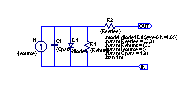
\includegraphics[width=\textwidth]{images/ltspice/singlecell.eps}
    \caption{%
        Schaltung        zur         Simulation        einer        Solarzelle
        gem\"ass        Abbildung       \ref{fig:circuit:solarCell}        von
        Seite     \pageref{fig:circuit:solarCell}. Die     Solarmodule     aus
        den     Abbildungen    \ref{fig:ltspice:module:cellBased:36x2}     und
        \ref{fig:ltspice:module:cellBased:72x1}  basieren auf  Zellen gem\"ass
        diesem Schaltschema.%
    }
    \label{fig:ltspice:solarCell}
\end{figure}

\begin{figure}[h!tb]
    \centering
    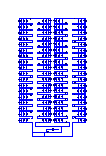
\includegraphics[width=\textwidth]{images/ltspice/module-72cells.eps}
    \caption{%
        Solarmodul     \"ahnlich     zu    Sunset     Solargenerator     AS150
        \cite{ref:solar:as150}, modelliert durch 2  parallele Str\"ange mit je
        36 Zellen gem\"ass Abbildung \ref{fig:ltspice:solarCell} in Serie.%
    }
    \label{fig:ltspice:module:cellBased:36x2}
\end{figure}

\begin{figure}[h!tb]
    \centering
    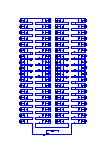
\includegraphics[width=\textwidth]{images/ltspice/module-72cells-series.eps}
    \caption{%
        Solarmodul   \"ahnlich   zu   Sunmodule  Pro-Series   XL   SW320   aus
        \cite{ref:solar:sunmodulePro},  modelliert durch  einen Strang  mit 72
        Zellen gem\"ass Abbildung \ref{fig:ltspice:solarCell} in Serie.%
    }
    \label{fig:ltspice:module:cellBased:72x1}
\end{figure}
\todo{Transistoren aus Schaltbildern entfernen, IN/OUT benennen, Abbildung sollte nur Modul sein}

%% **************************************************************************** %
\chapter{Verifikation des vereinfachten PV-Modul-Modells}
\label{app:simu:module:simple}
% **************************************************************************** %

Vereinfachtes  \code{LTspice}-Modell,  Verifikation anhand  von  verschiedenen
Plots.

\begin{figure}
    \begin{tikzpicture}
       \begin{scope}[x={(0mm,0mm)},y={(140mm,\textwidth)}]
           \begin{axis}[%
                   xmode=log,
                   height=65mm,
                   width=\textwidth,
                   at={(0,80mm)},
                   grid=both,
               ]
               \addplot[-,color=magenta] table {data/module-simple--frequency-response--mag.dat};
           \end{axis}
           \begin{axis}[%
                   xmode=log,
                   height=65mm,
                   width=\textwidth,
                   at={(0,0)},
                   grid=both,
               ]
               \addplot[-,color=red] table {data/module-simple--frequency-response--phase.dat};
           \end{axis}
       \end{scope}
   \end{tikzpicture}
   \caption{Frequenzgang f\"ur den Strom durch den MOSFET des vereinfachten Modells f\"ur ein Modul.}
   \label{fig:freqresponse:module:simple}
\end{figure}

\begin{figure}
    \begin{tikzpicture}
       \begin{scope}[x={(0mm,0mm)},y={(140mm,\textwidth)}]
           \begin{axis}[%
                   xmode=log,
                   height=65mm,
                   width=\textwidth,
                   at={(0,80mm)},
                   grid=both,
               ]
               \addplot[-,color=magenta] table {data/module-72cells--frequency-response--mag.dat};
           \end{axis}
           \begin{axis}[%
                   xmode=log,
                   height=65mm,
                   width=\textwidth,
                   at={(0,0)},
                   grid=both,
               ]
               \addplot[-,color=magenta] table {data/module-72cells--frequency-response--phase.dat};
           \end{axis}
       \end{scope}
   \end{tikzpicture}
   \caption{Frequenzgang f\"ur den Strom durch den MOSFET des Modells f\"ur ein Modul mit 72 Zellen}
   \label{fig:freqresponse:module:72cell}
\end{figure}

\begin{figure}
    \begin{tikzpicture}
       \begin{scope}[x={(0mm,0mm)},y={(140mm,\textwidth)}]
           \begin{axis}[%
                   xmode=log,
                   height=65mm,
                   width=\textwidth,
                   at={(0,80mm)},
                   grid=both,
               ]
               \addplot[-,color=magenta] table {data/module-simple--frequency-response--mag.dat};
               \addplot[-,color=blue] table {data/module-72cells--frequency-response--mag.dat};
           \end{axis}
           \begin{axis}[%
                   xmode=log,
                   height=65mm,
                   width=\textwidth,
                   at={(0,0)},
                   grid=both,
               ]
               \addplot[-,color=magenta] table {data/module-simple--frequency-response--phase.dat};
               \addplot[-,color=blue] table {data/module-72cells--frequency-response--phase.dat};
           \end{axis}
       \end{scope}
   \end{tikzpicture}
   \caption{Frequenzgang f\"ur den Strom durch den MOSFET des vereinfachten Modells f\"ur ein Modul.}
   \label{fig:freqresponse:module:simple}
\end{figure}

% **************************************************************************** %
\chapter{Erg\"anzende Simulationsergebnisse}
\label{app:simu:complementary}
% **************************************************************************** %


Dieses   Kapitel  beinhaltet   erg\"anzende  Simulationsergebnisse,   die  aus
Gr\"unden der \"Ubersichtlichkeit nicht im Hauptteil zu finden sind.


% ---------------------------------------------------------------------------- %
\section{Modul mit zwei parallelen Str\"angen}
\label{app:sec:simu:complementary:36x2}
% ---------------------------------------------------------------------------- %

\begin{figure}[h!tb]
    \centering
    \begin{tikzpicture}
       \begin{scope}[x={(0mm,0mm)},y={(120mm,0.95\textwidth)}]
           \begin{axis}[%
                   height=40mm,
                   width=\textwidth,
                   at={(0,70mm)},
                   grid=both,
                   xlabel=Zeit (\si{\micro\second}),
                   ylabel=Strom (\si{\ampere}),
                   %x unit=u,
                   change x base=true,
                   x SI prefix=micro,
               ]
               \addplot[-,color=blue] table {data/module-72cells--I-MOSFET--1000u.dat};
           \end{axis}
           \begin{axis}[%
                   height=40mm,
                   width=\textwidth,
                   at={(0,35mm)},
                   grid=both,
                   xlabel=Zeit (\si{\micro\second}),
                   ylabel=Spannung (\si{\volt}),
                   %x unit=u,
                   change x base=true,
                   x SI prefix=micro,
               ]
               \addplot[-,color=magenta] table {data/module-72cells--U-MOSFET--1000u.dat};
           \end{axis}
           \begin{axis}[%
                   height=40mm,
                   width=\textwidth,
                   at={(0,0)},
                   grid=both,
                   xlabel=Zeit (\si{\micro\second}),
                   ylabel=Leistung (\si{\watt}),
                   %x unit=u,
                   change x base=true,
                   x SI prefix=micro,
               ]
               \addplot[-,color=teal] table {data/module-72cells--P-MOSFET--1000u.dat};
           \end{axis}
       \end{scope}
   \end{tikzpicture}
   \caption{%
       Transientensimulation des Kurzschlussverfahrens f\"ur ASK mit einem $36 \times 2$-Modul%
   }
\end{figure}
\todo{``Abbilddung sowieso auf Seite diesunddas ist ein vergr\"osserter Ausschnitt eines Peaks aus dieser Simulation''}


\begin{figure}[h!tb]
    \centering
    \begin{tikzpicture}
       \begin{scope}[x={(0mm,0mm)},y={(120mm,0.95\textwidth)}]
           \begin{axis}[%
                   height=40mm,
                   width=\textwidth,
                   at={(0,70mm)},
                   grid=both,
                   xlabel=Zeit (\si{\micro\second}),
                   ylabel=Strom (\si{\ampere}),
                   %x unit=u,
                   change x base=true,
                   x SI prefix=micro,
               ]
               \addplot[-,color=blue] table {data/module-72cells-series--I-MOSFET--1000u.dat};
           \end{axis}
           \begin{axis}[%
                   height=40mm,
                   width=\textwidth,
                   at={(0,35mm)},
                   grid=both,
                   xlabel=Zeit (\si{\micro\second}),
                   ylabel=Spannung (\si{\volt}),
                   %x unit=u,
                   change x base=true,
                   x SI prefix=micro,
               ]
               \addplot[-,color=magenta] table {data/module-72cells-series--U-MOSFET--1000u.dat};
           \end{axis}
           \begin{axis}[%
                   height=40mm,
                   width=\textwidth,
                   at={(0,0)},
                   grid=both,
                   xlabel=Zeit (\si{\micro\second}),
                   ylabel=Leistung (\si{\watt}),
                   %x unit=u,
                   change x base=true,
                   x SI prefix=micro,
               ]
               \addplot[-,color=teal] table {data/module-72cells-series--P-MOSFET--1000u.dat};
           \end{axis}
       \end{scope}
   \end{tikzpicture}
   \caption{%
       Transientensimulation des Kurzschlussverfahrens f\"ur ASK mit einem $72 \times 1$-Modul%
   }
\end{figure}

\todo{``Abbilddung sowieso ist ein vergr\"osserter Ausschnitt eines Peaks aus dieser Simualtin}

% **************************************************************************** %
\chapter{Elektronische Datentr\"ager}
\label{app:electronicStorage}
% **************************************************************************** %



% -------------------------------------------------------- %
% Page  numbering continues,  but chapter  numbers are  no %
% longer  displayed. See  memoir  documentation  for  more %
% information.                                             %
% -------------------------------------------------------- %
\backmatter

% -------------------------------------------------------- %
% Bibliography: We  are using  the  IEEEtran package  from %
% Michael Shell                                            %
%                                                          %
% There  are  a  few  different  styles  in  the  IEEEtran %
% package.   We are  going to  use  one of  two of  those, %
% either in the sorted or unsorted variety.                %
%                                                          %
% The sorted  version sorts  bibliographic entries  in the %
% bibliography alphabetically, while  the unsorted version %
% lists bibliographic  entries in the order  in which they %
% were cited (first occurrence).                           %
% -------------------------------------------------------- %
%\bibliographystyle{bibliography/IEEEtranS} % sorted
\bibliographystyle{bibliography/IEEEtran} % unsorted
\bibliography{bibliography/references}
\end{document}
